% !TEX program = xelatex
\documentclass[UTF8,fontset=fandol,a4paper,11pt]{ctexart}
\usepackage[margin=21mm,top=23mm,bottom=22mm,headheight=16pt]{geometry}
\usepackage{amsmath,amssymb,mathtools,bm}
\usepackage{tikz}
\usetikzlibrary{arrows.meta,calc,angles,quotes,patterns}
\usepackage{xcolor,booktabs,array,longtable,enumitem,fancyhdr,needspace}
\usepackage[unicode,hidelinks]{hyperref}
\definecolor{ink}{HTML}{24343C}
\definecolor{accent}{HTML}{166A70}
\definecolor{muted}{HTML}{65747A}
\definecolor{rulegray}{HTML}{D4DDE0}
\definecolor{warm}{HTML}{966037}
\color{ink}
\setlength{\parindent}{2em}
\setlength{\parskip}{4pt}
\linespread{1.12}
\AtBeginDocument{\setlength{\abovedisplayskip}{6pt plus 2pt minus 1pt}
\setlength{\belowdisplayskip}{6pt plus 2pt minus 1pt}
\setlength{\abovedisplayshortskip}{0pt plus 1pt}
\setlength{\belowdisplayshortskip}{4pt plus 1pt}}
\setlist[enumerate]{label=(\arabic*),leftmargin=2.3em,itemsep=3pt,topsep=4pt}
\setlist[itemize]{leftmargin=2em,itemsep=2pt,topsep=4pt}
\allowdisplaybreaks[1]
\setlength{\emergencystretch}{2em}
\setcounter{secnumdepth}{0}
\providecommand{\tightlist}{\setlength{\itemsep}{0pt}\setlength{\parskip}{0pt}}
\ctexset{section={format=\Large\bfseries\color{accent},beforeskip=10pt,afterskip=9pt},
subsection={format=\normalsize\bfseries\color{accent},beforeskip=10pt,afterskip=4pt},
subsubsection={format=\normalsize\bfseries,beforeskip=8pt,afterskip=3pt}}
\pagestyle{fancy}
\fancyhf{}
\fancyhead[L]{\small\color{muted}物理学难题集萃}
% 页眉仅保留书名；版本名称只在封面显示。
\fancyfoot[L]{\small\color{muted}\chapterlabel}
\fancyfoot[R]{\small\thepage}
\renewcommand{\headrulewidth}{0.4pt}
\renewcommand{\footrulewidth}{0pt}
\newcommand{\dd}{\mathop{}\!\mathrm{d}}
\newcommand{\vect}[1]{\bm{#1}}
\newcommand{\tagline}[1]{\noindent{\small\color{muted}#1}\par}
\newcommand{\result}[1]{\begin{equation*}\boxed{#1}\end{equation*}}
\newcommand{\figcaption}[1]{\par\vspace{2pt}{\small\color{muted}#1}\par}
\newcommand{\teach}[2]{\Needspace{4\baselineskip}\subsection*{讲解要点与追问}#1\par\smallskip\noindent\textbf{追问：}#2\par}
\newcommand{\workarea}{\par\vspace{7mm}\noindent{\small\color{muted}作答区}\par\vspace{4mm}
\noindent\textcolor{rulegray}{\rule{\linewidth}{0.3pt}}\par\vspace{16mm}
\noindent\textcolor{rulegray}{\rule{\linewidth}{0.3pt}}\par\vspace{16mm}
\noindent\textcolor{rulegray}{\rule{\linewidth}{0.3pt}}\par\vspace{16mm}
\noindent\textcolor{rulegray}{\rule{\linewidth}{0.3pt}}}
\tikzset{axis/.style={-{Stealth[length=2mm]},thin,color=muted},
motion/.style={-{Stealth[length=2.3mm]},thick,color=accent},
force/.style={-{Stealth[length=2.3mm]},thick,color=warm},
traj/.style={thick,color=accent},guide/.style={dashed,thin,color=muted},
object/.style={thick,color=ink},every node/.style={font=\small}}\widowpenalty=10000\clubpenalty=10000\displaywidowpenalty=10000\newcommand{\chapterlabel}{近代物理第二章\quad 狭义相对论}







\hypersetup{pdftitle={近代物理第二章 狭义相对论·教师版},pdfauthor={}}

\begin{document}\pdfbookmark[0]{近代物理第二章 狭义相对论}{cover}

\thispagestyle{empty}\vspace*{22mm}

\noindent{\Huge\bfseries 物理学难题集萃}\par\vspace{10mm}

\noindent{\LARGE 近代物理第二章}\par\vspace{6mm}

\noindent{\LARGE 狭义相对论}\par\vspace{12mm}

\noindent{\Large\color{accent}教师版}\par\vspace{9mm}

\noindent\textcolor{accent}{\rule{\linewidth}{1pt}}\par\vspace{9mm}

\noindent 第1--19题\par\vfill\clearpage

\pdfbookmark[1]{题目目录}{contents}\section*{题目目录}

\begin{longtable}{@{}r p{113mm} r@{}}\toprule 题号 & 题目 & 页码\\\midrule

\hyperref[q:1]{1} & \hyperref[q:1]{飞船、定站与往返信号} & \pageref{q:1} \\

\hyperref[q:2]{2} & \hyperref[q:2]{运动中性线框的电荷与电偶极} & \pageref{q:2} \\

\hyperref[q:3]{3} & \hyperref[q:3]{两艘相向飞船的光信号} & \pageref{q:3} \\

\hyperref[q:4]{4} & \hyperref[q:4]{沿法线运动的平面镜} & \pageref{q:4} \\

\hyperref[q:5]{5} & \hyperref[q:5]{共同运动的介质界面} & \pageref{q:5} \\

\hyperref[q:6]{6} & \hyperref[q:6]{运动观察者所见的星空分布} & \pageref{q:6} \\

\hyperref[q:7]{7} & \hyperref[q:7]{运动点光源的接收强度} & \pageref{q:7} \\

\hyperref[q:8]{8} & \hyperref[q:8]{迎面反射镜返回的光功率} & \pageref{q:8} \\

\hyperref[q:9]{9} & \hyperref[q:9]{移动色散介质中的相速度} & \pageref{q:9} \\

\hyperref[q:10]{10} & \hyperref[q:10]{固有加速度恒定的星际航程} & \pageref{q:10} \\

\hyperref[q:11]{11} & \hyperref[q:11]{相对论火箭的质量比} & \pageref{q:11} \\

\hyperref[q:12]{12} & \hyperref[q:12]{光子火箭的巡航速度与燃料下限} & \pageref{q:12} \\

\hyperref[q:13]{13} & \hyperref[q:13]{恒固有加速度光子火箭的初始功率} & \pageref{q:13} \\

\hyperref[q:14]{14} & \hyperref[q:14]{高空缪子的寿命与磁偏转} & \pageref{q:14} \\

\hyperref[q:15]{15} & \hyperref[q:15]{电子与质子在非均匀磁场中的同轨运动} & \pageref{q:15} \\

\hyperref[q:16]{16} & \hyperref[q:16]{横向恒力作用下的相对论粒子} & \pageref{q:16} \\

\hyperref[q:17]{17} & \hyperref[q:17]{极端相对论粒子与双夸克模型} & \pageref{q:17} \\

\hyperref[q:18]{18} & \hyperref[q:18]{引力束缚尺度与模型的适用范围} & \pageref{q:18} \\

\hyperref[q:19]{19} & \hyperref[q:19]{引力红移、恒星参数与离子反冲} & \pageref{q:19} \\

\bottomrule\end{longtable}

\clearpage

\pdfbookmark[2]{第 1 题 飞船、定站与往返信号}{q1}

\section*{第 1 题\quad 飞船、定站与往返信号}\label{q:1}

一艘飞船以$0.8c$沿直线飞离地球。飞船中午经过地球时，船钟与地球钟均调为12:00。沿航向有一座相对地球静止的定站，站钟与地球钟按地球惯性系同步。船钟12:30时，飞船经过定站，并立即向地球发射无线电信号。
\begin{enumerate}
\item 飞船经过定站时，站钟读数是多少？
\item 地球系测得地球至定站的距离是多少？
\item 地球何时接收到信号？
\item 地球接收后立即回信。飞船保持匀速，何时按船钟接收到回信？
\end{enumerate}
取$c=3.0\times10^8\,\mathrm{m/s}$，忽略引力。

\begin{center}\begin{minipage}{.98\linewidth}\centering
\begin{tikzpicture}[scale=.9,transform shape]
\fill (0.00000,0.00000) circle(.035);\node[below] at (0.00000,0.00000) {地球};\fill (6.00000,0.00000) circle(.035);\node[below] at (6.00000,0.00000) {定站};\draw[guide] (0.00000,0.00000)--(6.00000,0.00000);\draw[object] (1.00000,0.75000)--(3.00000,0.75000)--(3.00000,1.45000)--(1.00000,1.45000)--(1.00000,0.75000);\node[anchor=center] at (2.00000,1.10000) {飞船};\draw[motion] (3.20000,1.10000)--(4.20000,1.10000);\node[above] at (3.70000,1.20000) {$0.8c$};\draw[<->,thin,color=muted] (0.00000,-1.00000)--(6.00000,-1.00000);\node[below] at (3.00000,-1.00000) {$L$};\node[above] at (3.00000,2.00000) {船钟30min经过定站};
\end{tikzpicture}
\figcaption{图近2.1\quad 同一地球惯性系内的地球、定站与匀速飞船。}
\end{minipage}\end{center}

\Needspace{8\baselineskip}

\pdfbookmark[3]{题型定位}{q1-h0}

\subsection*{题型定位}

四问分别涉及同步站钟、地球系空间长度、地球收信事件和船上收信本征时。先为$A,B,C,D$指定发生地点，再用地球、定站、飞船及两条光线贯穿四问；地球系计算给出全部交点，飞船系的完整解法用于说明同时长度与往返光程怎样随参考系改变。

\Needspace{8\baselineskip}

\pdfbookmark[3]{知识点}{q1-h1}

\subsection*{知识点}

匀速船钟同一世界线上的两事件满足$\Delta\tau=\Delta t/\gamma$。地球与定站的同步钟给坐标时，飞船系同时测量的两固定地点距离为$L/\gamma$。光在各惯性系中速度为$c$，收信由光线和接收者世界线求交。洛伦兹变换同时改变时间与位置，选取与发信事件同船时的地球事件，才得到飞船系的瞬时地球距离。

\Needspace{8\baselineskip}

\pdfbookmark[3]{物理图像}{q1-h2}

\subsection*{物理图像}

题图将地球与定站放在同一静止系。图A用$t,x$表示飞船和两条信号线，$B$发信、$C$地收并回信、$D$船收。图C列出三事件在两系的坐标，图B以$B$为局部船时零点，地球后退、飞船固定。图D专门选出与$B$在船系同时的地球事件$E$，使24光分进入追光方程的几何条件清楚可见。

\Needspace{8\baselineskip}

\pdfbookmark[3]{解题入口}{q1-h3}

\subsection*{解题入口}

先由船时30分钟求地球系50分钟，飞船的$x=0.8ct$随即确定$L$。在$B$写向后光线，到地球求$C$；在$C$写向前回信，与船线求$D$。最后将沿船线从出发至$D$的坐标时换成累计本征时。第二系解法从同时地球位置开始，两段光程分别求交。

\Needspace{8\baselineskip}

\pdfbookmark[3]{标准解法}{q1-h4}

\subsection*{标准解法}


以地球钟12:00为$t=0$，地球位置$x=0$，飞船沿$+x$运动。图近2.1中的定站位于$x=L$；地球、定站组成同一惯性系$S$，飞船系为$S'$。设$\beta=0.8$，
\[
\gamma=\frac1{\sqrt{1-\beta^2}}=\frac53,\qquad
x=\beta ct,\qquad \tau=\frac t\gamma.
\]
船钟沿飞船世界线累计本征时间$\tau$；定站的同步钟则直接给出$S$的坐标时。


（1）飞船与定站相遇事件记为$B$。船钟从12:00至12:30经过30min，故
\[
t_B=\gamma\tau_B=\frac53\times30=50\,\mathrm{min}.
\]
站钟与地球钟同步，因此相遇时站钟为$\boxed{12{:}50}$。站钟12:50是定站处同步钟的本地读数；远处钟面影像另含光传播延迟。

（2）飞船在$S$中经过的距离就是定站的地球坐标：
\[
\boxed{L=\beta ct_B
=0.8(3.0\times10^8)(50\times60)
=7.2\times10^{11}\,\mathrm m}.
\]
这等于40光分。若在飞船系同时测量地球与定站的距离，则为$L/\gamma=24$光分；两种长度使用不同的同时性条件。

\begin{center}\begin{minipage}{.98\linewidth}\centering
\begin{tikzpicture}[scale=.75,transform shape]
\draw[axis] (0.00000,0.00000)--(9.75000,0.00000);\draw[axis] (0.00000,0.00000)--(0.00000,7.85000);\node[below right] at (9.75000,0.00000) {$t/(50\,\mathrm{min})$};\node[above right] at (0.00000,7.85000) {$x/(50\,\text{光分})$};\draw[guide] (0.00000,0.80000)--(9.00000,0.80000);\node[right] at (9.00000,0.80000) {定站};\draw[traj] (0.00000,0.00000)--(9.00000,7.20000);\draw[force] (1.00000,0.80000)--(1.80000,0.00000);
\draw[force] (1.80000,0.00000)--(9.00000,7.20000);\fill (0.00000,0.00000) circle(.035);\node[below left] at (0.00000,0.00000) {$A$};\fill (1.00000,0.80000) circle(.035);\node[above left] at (1.00000,0.80000) {$B$};\fill (1.80000,0.00000) circle(.035);\node[below] at (1.80000,0.00000) {$C$};\fill (9.00000,7.20000) circle(.035);\node[above right] at (9.00000,7.20000) {$D$};\node[below right] at (6.00000,3.00000) {回信追船};\node[above left] at (4.00000,5.00000) {飞船 $x=0.8ct$};
\end{tikzpicture}
\figcaption{解图近2.1A\quad 发信、地收、船收分别由三条世界线求交。}
\end{minipage}\end{center}
（3）解图近2.1A中，$B\to C$为向地球传播的信号。它在$S$中满足
\[
x_{\rm sig}=L-c(t-t_B).
\]
到达$x=0$时，
\[
t_C=t_B+\frac Lc=50+40=90\,\mathrm{min}.
\]
因此地球接收时刻为$\boxed{13{:}30}$。50分钟给船从出发到过站的坐标时，40分钟给从定站到地球的信号光程；前一段对应船钟本征时，后一段按光线世界线定位接收事件。

（4）地球立即回信。解图近2.1A中$C\to D$的光线满足$x=c(t-t_C)$，与船的$x=\beta ct$相交：
\[
c(t_D-t_C)=\beta ct_D,\qquad
\boxed{t_D=\frac{t_C}{1-\beta}
=450\,\mathrm{min}}.
\]
地球系对应19:30。事件$D$在飞船上，故船钟自出发累计
\[
\tau_D=\frac{450}{5/3}=270\,\mathrm{min},
\qquad\boxed{\text{船钟接收时刻为 }16{:}30}.
\]
由图A的光程也可看到：$D$的位置为360光分；回信从$t=90$至450经过360min，确实走过360光分。

\begin{center}\begin{minipage}{.98\linewidth}\centering
\begin{tikzpicture}[scale=.72,transform shape]
\draw[axis] (0.00000,0.00000)--(8.85000,0.00000);\draw[axis] (0.00000,-7.80000)--(0.00000,1.45000);\node[below right] at (8.85000,0.00000) {$\Delta\tau/(30\,\mathrm{min})$};\node[above right] at (0.00000,1.45000) {$\xi/(30\,\text{光分})$};\draw[traj] (0.00000,0.00000)--(8.20000,0.00000);\node[above] at (4.00000,0.50000) {飞船固定 $\xi=0$};\draw[guide] (0.00000,-0.80000)--(8.00000,-7.20000);\node[below left] at (7.00000,-6.40000) {地球后退};\draw[force] (0.00000,0.00000)--(4.00000,-4.00000);
\draw[force] (4.00000,-4.00000)--(8.00000,0.00000);\fill (0.00000,0.00000) circle(.035);\node[above left] at (0.00000,0.00000) {$B$};\fill (4.00000,-4.00000) circle(.035);\node[below left] at (4.00000,-4.00000) {$C$};\fill (8.00000,0.00000) circle(.035);\node[above] at (8.00000,0.00000) {$D$};\node[left] at (1.00000,-2.00000) {120min};\node[right] at (6.00000,-2.00000) {120min};
\end{tikzpicture}
\figcaption{解图近2.1B\quad 从发信时起算，飞船系两段信号时间相等。}
\end{minipage}\end{center}
图C将刚求出的$B,C,D$事件在两系中的时间与地球系位置并列，图中三行分别对应发信、地收和船收。
\begin{center}\begin{minipage}{.98\linewidth}\centering
\begin{tikzpicture}[scale=.8,transform shape]
\node at (0,1) {事件};\node at (3,1) {$t$（分钟）};\node at (6,1) {$x/c$（分钟）};\node at (9,1) {$t'$（分钟）};\node at (0,0) {$B$，发信};\node at (3,0) {50};\node at (6,0) {40};\node at (9,0) {30};\node at (0,-1) {$C$，地收};\node at (3,-1) {90};\node at (6,-1) {0};\node at (9,-1) {150};\node at (0,-2) {$D$，船收};\node at (3,-2) {450};\node at (6,-2) {360};\node at (9,-2) {270};
\end{tikzpicture}
\figcaption{解图近2.1C\quad 同一组事件的地球坐标与飞船坐标时}
\end{minipage}\end{center}
飞船系的完整解法进一步说明，同时长度与两段追光时间怎样对应图A的同一组事件。解图近2.1B以飞船发信事件$B$为局部时间零点，飞船固定在$\xi=0$。在这个瞬间，地球位于$\xi=-L/\gamma=-24$光分，并以$-\beta c$运动。
这个同时地球位置可由洛伦兹变换明确选出。过站事件$B$为$(t,x/c)=(50,40)$分钟，故$t'_B=\gamma(t_B-\beta x_B/c)=30$分钟。地球上$x_E=0$，与$B$同船时要求$\gamma t_E=30$，所以$t_E=18$分钟，$x'_E/c=-\gamma\beta t_E=-24$分钟。图D的斜线连接这两个船系同时事件。
\begin{center}\begin{minipage}{.98\linewidth}\centering
\begin{tikzpicture}[scale=.8,transform shape]
\draw[axis] (0,0)--(8,0) node[right] {$t$};\draw[axis] (0,0)--(0,5) node[above] {$x/c$};\draw[traj] (0,0)--(6,4.8) node[above] {飞船};\draw[guide] (0,4)--(7,4) node[right] {定站};\draw[force] (1.8,0)--(5,4);\fill (5,4) circle(.04) node[above left] {$B:(50,40)$};\fill (1.8,0) circle(.04) node[below] {$E:(18,0)$};\node[above left] at (3,2.3) {$t'=30$分钟};\node[above] at (4,5.2) {斜线上的事件在船系同时};
\end{tikzpicture}
\figcaption{解图近2.1D\quad 地球事件$E$与过站事件$B$在飞船系同时}
\end{minipage}\end{center}向后的光以$-c$追地球，所以
\[
c\,\Delta\tau_1=\frac L\gamma+\beta c\,\Delta\tau_1,
\qquad
\Delta\tau_1=\frac{L}{\gamma c(1-\beta)}
=120\,\mathrm{min}.
\]
接收发生在船系$\xi=-c\Delta\tau_1$。地球回信后，光以$+c$回到不动的飞船，另需$\Delta\tau_2=\Delta\tau_1=120$min。飞船发信时已走30min，故最终船钟仍为$30+120+120=270$min。两条光路在船系用时相等，在地球系用时40min和360min；这与两个参考系对地球运动状态的判断一致。


\Needspace{8\baselineskip}

\pdfbookmark[3]{关键洞察}{q1-h5}

\subsection*{关键洞察}

坐标时来自同一惯性系内的同步钟，收到远处钟面信号则另含光传播延迟。$B$发生时，站钟读12:50，船钟读12:30；从地球传到$B$的钟面影像显示更早的地球时刻。地球系往返光传播时间为40和360分钟，船系则各120分钟，它们描述同一组事件在两套同时面上的交点。

\Needspace{8\baselineskip}

\pdfbookmark[3]{易错点}{q1-h6}

\subsection*{易错点}

站钟属于地球同步钟系，过站事件的站钟读数为12:50。回信发出时飞船已在定站之外，返程追赶距离由船的继续位移决定。地球系的450分钟与船钟的270分钟分别沿同一船线对应，所有地球收发事件另按其所在地点定位。$L/\gamma$与船系同时性配套，使用地球系飞行时间时则用$L$。

\Needspace{8\baselineskip}

\pdfbookmark[3]{课堂讲解建议}{q1-h7}

\subsection*{课堂讲解建议}

先让学生逐项指出出发、过站、地收、船收四事件发生在地球、定站还是飞船上，再标图A交点。回信阶段先在$t=90$分钟处画出飞船位置，解释为何回信追赶远超过40光分。随后在船系画地球后退，用图D选出与$B$同时的地球事件。最后比较图C两套坐标，要求用事件和参考系说清每一个钟读数的含义。

\Needspace{8\baselineskip}

\pdfbookmark[3]{变式训练}{q1-h8}

\subsection*{变式训练}

\begin{enumerate}
\Needspace{20\baselineskip}
\item 速度改为$\beta c$，到站时船钟增量为$\tau_s$，推导四问的一般式。
\textbf{解：}图V1用同样事件命名。$t_B=\gamma\tau_s,L=\beta c\gamma\tau_s$，向后信号在$t_C=t_B+L/c=(1+\beta)\gamma\tau_s$到地球。回信与$x=\beta ct$相交给$t_D=t_C/(1-\beta)$，所以$\tau_D=\tau_s(1+\beta)/(1-\beta)$。当$\beta\to0$且保持到站船时固定，定站距离同时趋零，往返延迟也趋零；固定距离的低速过程则属于另一组给定条件。
\begin{center}\begin{minipage}{.98\linewidth}\centering
\begin{tikzpicture}[scale=.8,transform shape]
\draw[axis] (0,0)--(10.7,0) node[right] {$\beta$};
\draw[axis] (0,0)--(0,3.2) node[above] {$\tau_D/\tau_s$};
\node[above] at (5,3.5) {固定到站船时下的回波时间比};
\draw[traj] plot coordinates {(0.000000000,0.300000000) (0.083333333,0.304026846) (0.166666667,0.308108108) (0.250000000,0.312244898) (0.333333333,0.316438356) (0.416666667,0.320689655) (0.500000000,0.325000000) (0.583333333,0.329370629) (0.666666667,0.333802817) (0.750000000,0.338297872) (0.833333333,0.342857143) (0.916666667,0.347482014) (1.000000000,0.352173913) (1.083333333,0.356934307) (1.166666667,0.361764706) (1.250000000,0.366666667) (1.333333333,0.371641791) (1.416666667,0.376691729) (1.500000000,0.381818182) (1.583333333,0.387022901) (1.666666667,0.392307692) (1.750000000,0.397674419) (1.833333333,0.403125000) (1.916666667,0.408661417) (2.000000000,0.414285714) (2.083333333,0.420000000) (2.166666667,0.425806452) (2.250000000,0.431707317) (2.333333333,0.437704918) (2.416666667,0.443801653) (2.500000000,0.450000000) (2.583333333,0.456302521) (2.666666667,0.462711864) (2.750000000,0.469230769) (2.833333333,0.475862069) (2.916666667,0.482608696) (3.000000000,0.489473684) (3.083333333,0.496460177) (3.166666667,0.503571429) (3.250000000,0.510810811) (3.333333333,0.518181818) (3.416666667,0.525688073) (3.500000000,0.533333333) (3.583333333,0.541121495) (3.666666667,0.549056604) (3.750000000,0.557142857) (3.833333333,0.565384615) (3.916666667,0.573786408) (4.000000000,0.582352941) (4.083333333,0.591089109) (4.166666667,0.600000000) (4.250000000,0.609090909) (4.333333333,0.618367347) (4.416666667,0.627835052) (4.500000000,0.637500000) (4.583333333,0.647368421) (4.666666667,0.657446809) (4.750000000,0.667741935) (4.833333333,0.678260870) (4.916666667,0.689010989) (5.000000000,0.700000000) (5.083333333,0.711235955) (5.166666667,0.722727273) (5.250000000,0.734482759) (5.333333333,0.746511628) (5.416666667,0.758823529) (5.500000000,0.771428571) (5.583333333,0.784337349) (5.666666667,0.797560976) (5.750000000,0.811111111) (5.833333333,0.825000000) (5.916666667,0.839240506) (6.000000000,0.853846154) (6.083333333,0.868831169) (6.166666667,0.884210526) (6.250000000,0.900000000) (6.333333333,0.916216216) (6.416666667,0.932876712) (6.500000000,0.950000000) (6.583333333,0.967605634) (6.666666667,0.985714286) (6.750000000,1.004347826) (6.833333333,1.023529412) (6.916666667,1.043283582) (7.000000000,1.063636364) (7.083333333,1.084615385) (7.166666667,1.106250000) (7.250000000,1.128571429) (7.333333333,1.151612903) (7.416666667,1.175409836) (7.500000000,1.200000000) (7.583333333,1.225423729) (7.666666667,1.251724138) (7.750000000,1.278947368) (7.833333333,1.307142857) (7.916666667,1.336363636) (8.000000000,1.366666667) (8.083333333,1.398113208) (8.166666667,1.430769231) (8.250000000,1.464705882) (8.333333333,1.500000000) (8.416666667,1.536734694) (8.500000000,1.575000000) (8.583333333,1.614893617) (8.666666667,1.656521739) (8.750000000,1.700000000) (8.833333333,1.745454545) (8.916666667,1.793023256) (9.000000000,1.842857143) (9.083333333,1.895121951) (9.166666667,1.950000000) (9.250000000,2.007692308) (9.333333333,2.068421053) (9.416666667,2.132432432) (9.500000000,2.200000000) (9.583333333,2.271428571) (9.666666667,2.347058824) (9.750000000,2.427272727) (9.833333333,2.512500000) (9.916666667,2.603225806) (10.000000000,2.700000000)};
\node[below] at (0,-.12) {$0$};
\node[below] at (5,-.12) {$0.4$};
\node[below] at (10,-.12) {$0.8$};
\end{tikzpicture}
\figcaption{变图近2.1V1\quad 固定到站船时下的回波时间比}
\end{minipage}\end{center}

\Needspace{20\baselineskip}
\item 地球收信后按地球钟等待5分钟再回信，其他数据保持，求船钟接收时刻。
\textbf{解：}图V2中地球回信事件由$t_C=90$改为95分钟，光线为$x=c(t-95)$。与$x=0.8ct$相交得$t_D=475$分钟，船时$\tau_D=475/(5/3)=285$分钟，即16:45。一般等待$\Delta t$使船钟接收增量为$\Delta t/[\gamma(1-\beta)]$，本题倍率为3，地球多等5分钟使船上多等15分钟。
\begin{center}\begin{minipage}{.98\linewidth}\centering
\begin{tikzpicture}[scale=.8,transform shape]
\draw[axis] (0,0)--(10.7,0);
\draw[axis] (0,0)--(0,3.2);
\draw[line width=7pt,color=accent] (1.0,0)--(1.0,2.430000000);
\node[below] at (1.0,-.14) {无等待};
\node[above] at (1.0,2.570000000) {$ 270 $};
\draw[line width=7pt,color=accent] (9.0,0)--(9.0,2.565000000);
\node[below] at (9.0,-.14) {地球等5分钟};
\node[above] at (9.0,2.705000000) {$ 285 $};
\end{tikzpicture}
\figcaption{变图近2.1V2\quad 最终船时累计（分钟）：等待被追光过程放大}
\end{minipage}\end{center}

\Needspace{20\baselineskip}
\item 到站船时仍为30分钟，要求船钟15:00前收到回信，速度应满足什么条件？
\textbf{解：}图V3中允许$\tau_D\le180$分钟。代一般式得$(1+\beta)/(1-\beta)\le6$，由于$0\le\beta<1$，可解得$\beta\le5/7$。到站船时固定，所以不同速度对应不同定站距离$L=\beta c\gamma\tau_s$；最大速度时$L/c=75/\sqrt6$分钟，约30.619光分。若固定定站40光分，便需另用该距离条件计算到站时刻。
\begin{center}\begin{minipage}{.98\linewidth}\centering
\begin{tikzpicture}[scale=.8,transform shape]
\draw[axis] (-2.5,0)--(2.7,0) node[right] {$x$};
\draw[axis] (0,-2.5)--(0,2.7) node[above] {$y$};
\draw[traj] (-2.300000000,-0.000000000)--(2.300000000,0.000000000);
\node[above] at (2.300000000,0.150000000) {$\tau_D\le180$分钟};
\end{tikzpicture}
\figcaption{变图近2.1V3\quad $\beta\le5/7$，到站船时固定30分钟}
\end{minipage}\end{center}

\Needspace{20\baselineskip}
\item 只给地球到定站40光分，飞船速度仍0.8$c$，重新求到站船时和最终收信船时。
\textbf{解：}图V4中地球系飞行时间$t_B=(L/c)/\beta=40/0.8=50$分钟，船时$\tau_B=t_B/\gamma=30$分钟。地球收信$t_C=50+40=90$，船收地球系$t_D=90/(1-0.8)=450$，故船时270分钟。时间与距离两种给定方式在本组数值下选中同一条世界线及同一过站事件。
\begin{center}\begin{minipage}{.98\linewidth}\centering
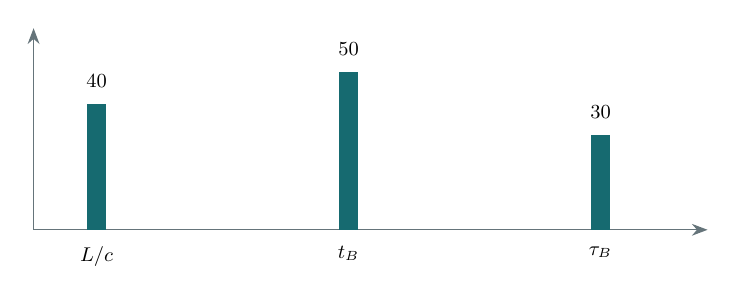
\begin{tikzpicture}[scale=.8,transform shape]
\draw[axis] (0,0)--(10.7,0);
\draw[axis] (0,0)--(0,3.2);
\draw[line width=7pt,color=accent] (1.0,0)--(1.0,2.000000000);
\node[below] at (1.0,-.14) {$L/c$};
\node[above] at (1.0,2.140000000) {$ 40 $};
\draw[line width=7pt,color=accent] (5.0,0)--(5.0,2.500000000);
\node[below] at (5.0,-.14) {$t_B$};
\node[above] at (5.0,2.640000000) {$ 50 $};
\draw[line width=7pt,color=accent] (9.0,0)--(9.0,1.500000000);
\node[below] at (9.0,-.14) {$\tau_B$};
\node[above] at (9.0,1.640000000) {$ 30 $};
\end{tikzpicture}
\figcaption{变图近2.1V4\quad 固定距离推得地球飞行时和船时（分钟）}
\end{minipage}\end{center}

\Needspace{20\baselineskip}
\item 在过站事件$B$，飞船或站上看见的地球钟面影像显示几点？与船系同时的地球钟又显示几点？
\textbf{解：}图V5中从地球发出的光需40分钟到达$B$，因此影像对应地球$t=50-40=10$分钟，即12:10。船系同时地球事件$E$满足$t'_E=t'_B=30$分钟；地球上$x_E=0$，故$\gamma t_E=30$，得$t_E=18$分钟，即12:18。站钟在$B$的直接读数12:50属于地球系同步时，三种读数由光路、同时面和本地钟分别给出。
\begin{center}\begin{minipage}{.98\linewidth}\centering
\begin{tikzpicture}[scale=.8,transform shape]
\node at (0,1) {地球发出钟面光};\node at (5,1) {过站事件$B$};\draw[motion] (0,.5)--(5,.5) node[midway,above] {40光分};\node at (0,0) {12:10};\node at (5,0) {站钟12:50，船钟12:30};\node at (2.5,-1) {船系同时地球钟：12:18};
\end{tikzpicture}
\figcaption{变图近2.1V5\quad 收到的影像与同时地球事件分别由光线和同时面决定}
\end{minipage}\end{center}

\Needspace{20\baselineskip}
\item 飞船在定站$B$发信后立即停留，忽略减速过程的时间与距离，地球仍立即回信。最终船钟何时收到回信？
\textbf{解：}图V6中$B$之前船钟累计30分钟；从$B$起飞船与定站静止，船钟随后按地球系同样速率走。地球在$t_C=90$分钟回信，回到40光分外的定站需40分钟，于$t_D=130$分钟到达。停留阶段经历$130-50=80$分钟，所以船钟总增量$30+80=110$分钟，即13:50。钟的整段累计按两段运动历史分别计算。
\begin{center}\begin{minipage}{.98\linewidth}\centering
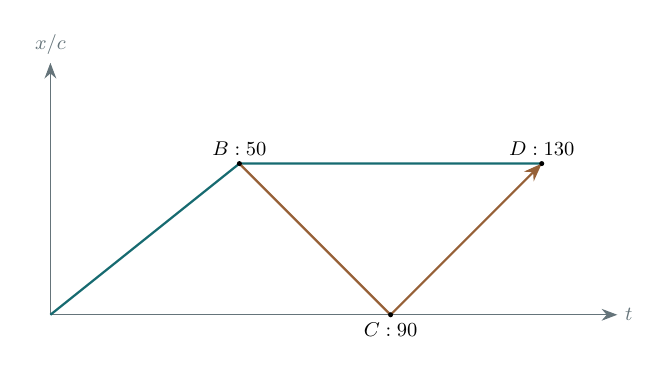
\begin{tikzpicture}[scale=.8,transform shape]
\draw[axis] (0,0)--(9,0) node[right] {$t$};\draw[axis] (0,0)--(0,4) node[above] {$x/c$};\draw[traj] (0,0)--(3,2.4)--(7.8,2.4);\draw[force] (3,2.4)--(5.4,0)--(7.8,2.4);\fill (3,2.4) circle(.04) node[above] {$B:50$};\fill (5.4,0) circle(.04) node[below] {$C:90$};\fill (7.8,2.4) circle(.04) node[above] {$D:130$};
\end{tikzpicture}
\figcaption{变图近2.1V6\quad 发信后停在定站，返程光不再追赶远离飞船}
\end{minipage}\end{center}

\Needspace{20\baselineskip}
\item 定站钟比地球同步钟快7分钟，其他空间位置和船速保持，求过站站钟读数及地球收信时刻。
\textbf{解：}图V7中站钟只改变零点，坐标时仍由地球同步钟给出。过站事件为$t_B=50$分钟，站钟显示12:57；发信位置仍40光分，地球收到信号仍是13:30。初始钟面偏置改变读数，与钟的速率、航程和光传播时间分别进入计算。若已知站钟偏置，应先减去7分钟恢复地球坐标时。
\begin{center}\begin{minipage}{.98\linewidth}\centering
\begin{tikzpicture}[scale=.8,transform shape]
\draw[axis] (0,0)--(10.7,0);
\draw[axis] (0,0)--(0,3.2);
\draw[line width=7pt,color=accent] (1.0,0)--(1.0,2.250000000);
\node[below] at (1.0,-.14) {同步站钟增量};
\node[above] at (1.0,2.390000000) {$ 50 $};
\draw[line width=7pt,color=accent] (9.0,0)--(9.0,2.565000000);
\node[below] at (9.0,-.14) {快7分钟的站钟};
\node[above] at (9.0,2.705000000) {$ 57 $};
\end{tikzpicture}
\figcaption{变图近2.1V7\quad 同一过站事件的两个钟面读数，单位分钟}
\end{minipage}\end{center}

\Needspace{20\baselineskip}
\item 飞船在定站附近连续发出等船时间隔的脉冲，地球逐个立即回传。求地球接收间隔、船上回波间隔及回波脉冲的重复频率比。
\textbf{解：}图V8中任一发射船时$\tau$对应地球收信$t_C=\gamma(1+\beta)\tau$，船收回波$\tau_D=(1+\beta)\tau/(1-\beta)$。故地球间隔为$\kappa\Delta\tau$、船上回波间隔为$\kappa^2\Delta\tau$，其中$\kappa=\sqrt{(1+\beta)/(1-\beta)}$。0.8$c$时$\kappa=3$，回波间隔变为9倍，因此回波脉冲的重复频率为发射重复频率的1/9。两段远离的光传播依次使接收脉冲间隔乘上同一个远离因子。
\begin{center}\begin{minipage}{.98\linewidth}\centering
\begin{tikzpicture}[scale=.8,transform shape]
\draw[axis] (0,0)--(10.7,0) node[right] {发射船时（分钟）};
\draw[axis] (0,0)--(0,3.2) node[above] {接收时间（分钟）};
\node[above] at (5,3.5) {实线地球收信；虚线船上收回波};
\draw[traj] plot coordinates {(0.000000000,0.000000000) (0.083333333,0.007500000) (0.166666667,0.015000000) (0.250000000,0.022500000) (0.333333333,0.030000000) (0.416666667,0.037500000) (0.500000000,0.045000000) (0.583333333,0.052500000) (0.666666667,0.060000000) (0.750000000,0.067500000) (0.833333333,0.075000000) (0.916666667,0.082500000) (1.000000000,0.090000000) (1.083333333,0.097500000) (1.166666667,0.105000000) (1.250000000,0.112500000) (1.333333333,0.120000000) (1.416666667,0.127500000) (1.500000000,0.135000000) (1.583333333,0.142500000) (1.666666667,0.150000000) (1.750000000,0.157500000) (1.833333333,0.165000000) (1.916666667,0.172500000) (2.000000000,0.180000000) (2.083333333,0.187500000) (2.166666667,0.195000000) (2.250000000,0.202500000) (2.333333333,0.210000000) (2.416666667,0.217500000) (2.500000000,0.225000000) (2.583333333,0.232500000) (2.666666667,0.240000000) (2.750000000,0.247500000) (2.833333333,0.255000000) (2.916666667,0.262500000) (3.000000000,0.270000000) (3.083333333,0.277500000) (3.166666667,0.285000000) (3.250000000,0.292500000) (3.333333333,0.300000000) (3.416666667,0.307500000) (3.500000000,0.315000000) (3.583333333,0.322500000) (3.666666667,0.330000000) (3.750000000,0.337500000) (3.833333333,0.345000000) (3.916666667,0.352500000) (4.000000000,0.360000000) (4.083333333,0.367500000) (4.166666667,0.375000000) (4.250000000,0.382500000) (4.333333333,0.390000000) (4.416666667,0.397500000) (4.500000000,0.405000000) (4.583333333,0.412500000) (4.666666667,0.420000000) (4.750000000,0.427500000) (4.833333333,0.435000000) (4.916666667,0.442500000) (5.000000000,0.450000000) (5.083333333,0.457500000) (5.166666667,0.465000000) (5.250000000,0.472500000) (5.333333333,0.480000000) (5.416666667,0.487500000) (5.500000000,0.495000000) (5.583333333,0.502500000) (5.666666667,0.510000000) (5.750000000,0.517500000) (5.833333333,0.525000000) (5.916666667,0.532500000) (6.000000000,0.540000000) (6.083333333,0.547500000) (6.166666667,0.555000000) (6.250000000,0.562500000) (6.333333333,0.570000000) (6.416666667,0.577500000) (6.500000000,0.585000000) (6.583333333,0.592500000) (6.666666667,0.600000000) (6.750000000,0.607500000) (6.833333333,0.615000000) (6.916666667,0.622500000) (7.000000000,0.630000000) (7.083333333,0.637500000) (7.166666667,0.645000000) (7.250000000,0.652500000) (7.333333333,0.660000000) (7.416666667,0.667500000) (7.500000000,0.675000000) (7.583333333,0.682500000) (7.666666667,0.690000000) (7.750000000,0.697500000) (7.833333333,0.705000000) (7.916666667,0.712500000) (8.000000000,0.720000000) (8.083333333,0.727500000) (8.166666667,0.735000000) (8.250000000,0.742500000) (8.333333333,0.750000000) (8.416666667,0.757500000) (8.500000000,0.765000000) (8.583333333,0.772500000) (8.666666667,0.780000000) (8.750000000,0.787500000) (8.833333333,0.795000000) (8.916666667,0.802500000) (9.000000000,0.810000000) (9.083333333,0.817500000) (9.166666667,0.825000000) (9.250000000,0.832500000) (9.333333333,0.840000000) (9.416666667,0.847500000) (9.500000000,0.855000000) (9.583333333,0.862500000) (9.666666667,0.870000000) (9.750000000,0.877500000) (9.833333333,0.885000000) (9.916666667,0.892500000) (10.000000000,0.900000000)};
\draw[dashed,thick,color=warm] plot coordinates {(0.000000000,0.000000000) (0.083333333,0.022500000) (0.166666667,0.045000000) (0.250000000,0.067500000) (0.333333333,0.090000000) (0.416666667,0.112500000) (0.500000000,0.135000000) (0.583333333,0.157500000) (0.666666667,0.180000000) (0.750000000,0.202500000) (0.833333333,0.225000000) (0.916666667,0.247500000) (1.000000000,0.270000000) (1.083333333,0.292500000) (1.166666667,0.315000000) (1.250000000,0.337500000) (1.333333333,0.360000000) (1.416666667,0.382500000) (1.500000000,0.405000000) (1.583333333,0.427500000) (1.666666667,0.450000000) (1.750000000,0.472500000) (1.833333333,0.495000000) (1.916666667,0.517500000) (2.000000000,0.540000000) (2.083333333,0.562500000) (2.166666667,0.585000000) (2.250000000,0.607500000) (2.333333333,0.630000000) (2.416666667,0.652500000) (2.500000000,0.675000000) (2.583333333,0.697500000) (2.666666667,0.720000000) (2.750000000,0.742500000) (2.833333333,0.765000000) (2.916666667,0.787500000) (3.000000000,0.810000000) (3.083333333,0.832500000) (3.166666667,0.855000000) (3.250000000,0.877500000) (3.333333333,0.900000000) (3.416666667,0.922500000) (3.500000000,0.945000000) (3.583333333,0.967500000) (3.666666667,0.990000000) (3.750000000,1.012500000) (3.833333333,1.035000000) (3.916666667,1.057500000) (4.000000000,1.080000000) (4.083333333,1.102500000) (4.166666667,1.125000000) (4.250000000,1.147500000) (4.333333333,1.170000000) (4.416666667,1.192500000) (4.500000000,1.215000000) (4.583333333,1.237500000) (4.666666667,1.260000000) (4.750000000,1.282500000) (4.833333333,1.305000000) (4.916666667,1.327500000) (5.000000000,1.350000000) (5.083333333,1.372500000) (5.166666667,1.395000000) (5.250000000,1.417500000) (5.333333333,1.440000000) (5.416666667,1.462500000) (5.500000000,1.485000000) (5.583333333,1.507500000) (5.666666667,1.530000000) (5.750000000,1.552500000) (5.833333333,1.575000000) (5.916666667,1.597500000) (6.000000000,1.620000000) (6.083333333,1.642500000) (6.166666667,1.665000000) (6.250000000,1.687500000) (6.333333333,1.710000000) (6.416666667,1.732500000) (6.500000000,1.755000000) (6.583333333,1.777500000) (6.666666667,1.800000000) (6.750000000,1.822500000) (6.833333333,1.845000000) (6.916666667,1.867500000) (7.000000000,1.890000000) (7.083333333,1.912500000) (7.166666667,1.935000000) (7.250000000,1.957500000) (7.333333333,1.980000000) (7.416666667,2.002500000) (7.500000000,2.025000000) (7.583333333,2.047500000) (7.666666667,2.070000000) (7.750000000,2.092500000) (7.833333333,2.115000000) (7.916666667,2.137500000) (8.000000000,2.160000000) (8.083333333,2.182500000) (8.166666667,2.205000000) (8.250000000,2.227500000) (8.333333333,2.250000000) (8.416666667,2.272500000) (8.500000000,2.295000000) (8.583333333,2.317500000) (8.666666667,2.340000000) (8.750000000,2.362500000) (8.833333333,2.385000000) (8.916666667,2.407500000) (9.000000000,2.430000000) (9.083333333,2.452500000) (9.166666667,2.475000000) (9.250000000,2.497500000) (9.333333333,2.520000000) (9.416666667,2.542500000) (9.500000000,2.565000000) (9.583333333,2.587500000) (9.666666667,2.610000000) (9.750000000,2.632500000) (9.833333333,2.655000000) (9.916666667,2.677500000) (10.000000000,2.700000000)};
\node[below] at (0,-.12) {$0$};
\node[below] at (5,-.12) {$15$};
\node[below] at (10,-.12) {$30$};
\end{tikzpicture}
\figcaption{变图近2.1V8\quad 实线地球收信；虚线船上收回波}
\end{minipage}\end{center}
\end{enumerate}

\Needspace{13\baselineskip}

\pdfbookmark[2]{第 2 题 运动中性线框的电荷与电偶极}{q2}

\section*{第 2 题\quad 运动中性线框的电荷与电偶极}\label{q:2}

正方形绝缘线框$ABCD$在自身静止系$S'$中边长为$L$，$AB$沿$+x'$，$BC$沿$-y'$。许多电荷均为$q>0$的小球沿$A\to B\to C\to D\to A$以恒定速率$u$运动，$S'$同时测得相邻球间距为$a\ll L$。框上的固定线电荷均匀分布，使各边在$S'$中均为电中性。采用连续线密度近似，忽略四角及离散计数涨落。

线框整体以$v$沿实验室系$S$的$+x$运动，$0<u,v<c$。在$S$中，框内有均匀外电场
\[
\boldsymbol E=-E\cos\theta\,\hat{\boldsymbol y}
+E\sin\theta\,\hat{\boldsymbol z},
\qquad 0\le\theta\le\frac\pi2,
\]
其中框面为$xy$面，$\hat{\boldsymbol z}=\hat{\boldsymbol x}\times\hat{\boldsymbol y}$；实验室外磁场为零。取上边$AB$为$y=L$、下边$CD$为$y=0$。求$S$中各边球间距、各边净电荷、框和球所受电力矩及外场电势能。

\begin{center}\begin{minipage}{.98\linewidth}\centering
\begin{tikzpicture}[scale=.9,transform shape]
\draw[object] (0.00000,0.00000)--(4.00000,0.00000)--(4.00000,2.80000)--(0.00000,2.80000)--(0.00000,0.00000);\node[above left] at (0.00000,2.80000) {$A$};\node[above right] at (4.00000,2.80000) {$B$};\node[below right] at (4.00000,0.00000) {$C$};\node[below left] at (0.00000,0.00000) {$D$};\draw[object] (0.35000,2.80000) circle(0.05500);\draw[object] (1.17500,2.80000) circle(0.05500);\draw[object] (2.00000,2.80000) circle(0.05500);\draw[object] (2.82500,2.80000) circle(0.05500);\draw[object] (3.65000,2.80000) circle(0.05500);\draw[object] (0.35000,0.00000) circle(0.05500);\draw[object] (1.17500,0.00000) circle(0.05500);\draw[object] (2.00000,0.00000) circle(0.05500);\draw[object] (2.82500,0.00000) circle(0.05500);\draw[object] (3.65000,0.00000) circle(0.05500);\draw[object] (0.00000,0.50000) circle(0.05500);\draw[object] (0.00000,1.30000) circle(0.05500);\draw[object] (0.00000,2.10000) circle(0.05500);\draw[object] (4.00000,0.50000) circle(0.05500);\draw[object] (4.00000,1.30000) circle(0.05500);\draw[object] (4.00000,2.10000) circle(0.05500);\draw[motion] (0.80000,3.35000)--(2.00000,3.35000);\node[above] at (1.40000,3.45000) {$u$};\draw[motion] (3.20000,-0.55000)--(2.00000,-0.55000);\node[below] at (2.60000,-0.60000) {$u$};\draw[<->,thin,color=muted] (0.00000,-1.30000)--(4.00000,-1.30000);\node[below] at (2.00000,-1.30000) {$L$};\draw[<->,thin,color=muted] (-1.00000,0.00000)--(-1.00000,2.80000);\node[left] at (-1.00000,1.40000) {$L$};\draw[motion] (5.00000,1.00000)--(6.20000,1.00000);\node[above] at (5.60000,1.10000) {$v$};\node[above] at (2.00000,4.00000) {固定负线电荷；球电荷 $q>0$};
\end{tikzpicture}
\figcaption{图近2.2\quad 框系的中性电流环及其整体平动方向。}
\end{minipage}\end{center}

\Needspace{8\baselineskip}

\pdfbookmark[3]{题型定位}{q2-h0}

\subsection*{题型定位}

在实验室同一时刻清点开放框边内的流动电荷，求中性电流环的局部电荷分离。四问依次求间距、边电荷、力偶和外势能。固定载荷属于同一组物质，流动小球则不断进出框边；同时切片使它们的变换方式有别。后两问按图中电场面内、面外分量分别作点积与叉积。

\Needspace{8\baselineskip}

\pdfbookmark[3]{知识点}{q2-h1}

\subsection*{知识点}

水平球列的本征间距$a_0=\gamma_u a$，实验室同时测量再按球的合成速度收缩，得到$a/[\gamma_v(1\pm uv/c^2)]$。横向同一竖边相邻两球$x'$相同，其同时性条件一致，间距$a$保持。固定边的总电荷不变，密度和电流则组成四电流共同变换。中性系统在均匀外场合力为零，可有非零偶极力矩，外势能为$-\boldsymbol p\cdot\boldsymbol E$。

\Needspace{8\baselineskip}

\pdfbookmark[3]{物理图像}{q2-h2}

\subsection*{物理图像}

题图给出球沿框的循环方向与框沿$+x$平动。图A并列同长水平边上的不同球间距及$+Q,-Q$，两竖边中性。图C列出实验室同时清点的球数与固定电荷，显示整框净量为零。图B、D在$y,z$截面分解外电场，$\boldsymbol p$沿$+y$，面外分量贡献绕$x$力偶，面内反向分量给正外势能。

\Needspace{8\baselineskip}

\pdfbookmark[3]{解题入口}{q2-h3}

\subsection*{解题入口}

先为四边球的速度标方向，在水平边先由$a$求局部本征间距，再按速度合成求实验室球距。用实验室框长除球距，计算开放边在同一时刻容纳的球电荷，与固定线电荷相加。得到上下等量异号电荷后，将均匀外力作用点取在各边中点，用叉积求力矩、点积或外电势求势能。

\Needspace{8\baselineskip}

\pdfbookmark[3]{标准解法}{q2-h4}

\subsection*{标准解法}


图近2.2中，固定线电荷跟随框运动，球还沿框循环。计算边上的净电荷，在同一$S$时刻分别清点固定载荷与流动球列。固定载荷属于同一条框边，球却不断流入、流出，固定载荷保持同一物质集合，边内球数则由同时密度与边长共同确定。记
\[
\gamma_v=\frac1{\sqrt{1-v^2/c^2}},\qquad
\gamma_u=\frac1{\sqrt{1-u^2/c^2}}.
\]
实验室清点对应一次同时切片。洛伦兹关系$t=\gamma_v(t'+vx'/c^2)$给$S$同时面$t'=t/\gamma_v-vx'/c^2$。沿$AB$的球列在框系满足$x'_k=ut'+ka$，不同$x'$所取球事件的$t'$也不同；$CD$的环流速度符号相反。竖边相邻球的$x'$相同，同一$t$对应同一$t'$，且横向坐标保持。下面的两次长度变换具体算出这些同时取点条件所给的球距。

（1）先看$AB$上的直线运动。局部与球共动的惯性系中球间距为$a_0=\gamma_u a$。该共动系用于这条直线段，四边的球速方向分别由框上的环流确定。球在$S$中的速度为
\[
w_{AB}=\frac{u+v}{1+uv/c^2},\qquad
\gamma(w_{AB})=\gamma_u\gamma_v(1+uv/c^2).
\]
把球的本征间距除以其在$S$中的洛伦兹因子，得到
\[
a_{AB}=\frac{a_0}{\gamma(w_{AB})}
=\frac{\gamma_u a}{\gamma_u\gamma_v(1+uv/c^2)}.
\]
因此$S$同时测得
\[
\boxed{a_{AB}=\frac a{\gamma_v(1+uv/c^2)}}.
\]
在$CD$上令$u\to-u$，得
\[
\boxed{a_{CD}=\frac a{\gamma_v(1-uv/c^2)}}.
\]
两条竖边同一边上各球具有相同的$x'$，因此同时性变换不会在这一边的两球之间引入$t'$差；$y=y'$不变，故
\[
\boxed{a_{BC}=a_{DA}=a}.
\]
竖边球在$S$中同时具有平动速度$v$和竖直速度分量$\pm u/\gamma_v$。

\begin{center}\begin{minipage}{.98\linewidth}\centering
\begin{tikzpicture}[scale=.74,transform shape]
\draw[object] (0.00000,0.00000)--(4.00000,0.00000)--(4.00000,2.80000)--(0.00000,2.80000)--(0.00000,0.00000);\node[above left] at (0.00000,2.80000) {$A$};\node[above right] at (4.00000,2.80000) {$B$};\node[below right] at (4.00000,0.00000) {$C$};\node[below left] at (0.00000,0.00000) {$D$};\draw[object] (0.35000,2.80000) circle(0.05500);\draw[object] (0.90000,2.80000) circle(0.05500);\draw[object] (1.45000,2.80000) circle(0.05500);\draw[object] (2.00000,2.80000) circle(0.05500);\draw[object] (2.55000,2.80000) circle(0.05500);\draw[object] (3.10000,2.80000) circle(0.05500);\draw[object] (3.65000,2.80000) circle(0.05500);\draw[object] (0.35000,0.00000) circle(0.05500);\draw[object] (1.45000,0.00000) circle(0.05500);\draw[object] (2.55000,0.00000) circle(0.05500);\draw[object] (3.65000,0.00000) circle(0.05500);\draw[object] (0.00000,0.50000) circle(0.05500);\draw[object] (0.00000,1.30000) circle(0.05500);\draw[object] (0.00000,2.10000) circle(0.05500);\draw[object] (4.00000,0.50000) circle(0.05500);\draw[object] (4.00000,1.30000) circle(0.05500);\draw[object] (4.00000,2.10000) circle(0.05500);\draw[motion] (0.80000,3.35000)--(2.00000,3.35000);\node[above] at (1.40000,3.45000) {$u$};\draw[motion] (3.20000,-0.55000)--(2.00000,-0.55000);\node[below] at (2.60000,-0.60000) {$u$};\node[above] at (2.00000,3.90000) {$+Q$};\node[below] at (2.00000,-1.20000) {$-Q$};\node[left] at (-0.50000,1.40000) {0};\node[right] at (4.50000,1.40000) {0};\node[above] at (2.00000,4.50000) {$AB,CD$长均为 $L/\gamma_v$};\node[above] at (7.00000,2.80000) {$a_{AB}=a/[\gamma_v(1+uv/c^2)]$};\node[above] at (7.00000,1.50000) {$a_{CD}=a/[\gamma_v(1-uv/c^2)]$};\node[above] at (7.00000,0.20000) {两竖边球间距仍为 $a$};\node[below] at (5.50000,-1.80000) {连续密度与球数变化示意；总电荷为零};
\end{tikzpicture}
\figcaption{解图近2.2A\quad 实验室同时计数产生上下等量异号的净电荷。}
\end{minipage}\end{center}
（2）解图近2.2A中，水平框边在$S$中长$L/\gamma_v$，但其球间距还含$1\pm uv/c^2$。每一条固定框边的总电荷均为
\[
Q_{\rm fixed}=-\frac{Lq}{a}.
\]
这个量是同一组固定载荷的电荷，不随惯性系变化。上边球的总电荷则为
\[
Q_{AB,\rm ball}=\frac{L/\gamma_v}{a_{AB}}q
=\frac{Lq}{a}(1+uv/c^2).
\]
相加即
\[
\boxed{Q_{AB}=Q=\frac{Lquv}{ac^2}},\qquad
\boxed{Q_{CD}=-Q},\qquad
\boxed{Q_{BC}=Q_{DA}=0}.
\]
图C将实验室同一时刻各边的球数与固定电量并列。上下净电荷等量异号，全框总电荷仍为零。竖边长$L$且球距$a$，固定与运动电荷仍恰好抵消。
\begin{center}\begin{minipage}{.98\linewidth}\centering
\begin{tikzpicture}[scale=.8,transform shape]
\node at (0,1) {实验室同一时刻};\node at (4,1) {球数};\node at (8,1) {固定电量};\node at (0,0) {$AB$};\node at (4,0) {$(L/a)(1+uv/c^2)$};\node at (8,0) {$-Lq/a$};\node at (0,-1) {$CD$};\node at (4,-1) {$(L/a)(1-uv/c^2)$};\node at (8,-1) {$-Lq/a$};\node at (0,-2) {$BC,DA$各边};\node at (4,-2) {$L/a$};\node at (8,-2) {$-Lq/a$};
\end{tikzpicture}
\figcaption{解图近2.2C\quad 边内流动球数改变；同一组固定载荷总电量保持}
\end{minipage}\end{center}

局部四电流将上述球距效应写成密度与电流的变换：在$S'$上边，总线电荷密度$\lambda'=0$，电流$j'_x=qu/a$。沿$x$变换后
\[
\lambda=\gamma_v\!\left(\lambda'+\frac{v j'_x}{c^2}\right)
=\gamma_v\frac{quv}{ac^2}.
\]
再乘实验室边长$L/\gamma_v$，得到同一个$Q$；下边电流反向，故电荷反号。这也说明框长收缩与球列同时密度共同决定实验室边电荷。

\begin{center}\begin{minipage}{.98\linewidth}\centering
\begin{tikzpicture}[scale=.88,transform shape]
\draw[axis] (0.00000,0.00000)--(3.95000,0.00000);\draw[axis] (0.00000,0.00000)--(0.00000,3.25000);\node[below right] at (3.95000,0.00000) {$y$};\node[above right] at (0.00000,3.25000) {$z$};\draw[thin,color=muted] (-3.00000,0.00000)--(0.00000,0.00000);\draw[motion] (0.00000,0.00000)--(3.00000,0.00000);\node[above] at (2.00000,0.20000) {$\boldsymbol p=QL\hat y$};\draw[force] (0.00000,0.00000)--(-2.20000,2.20000);\node[above left] at (-2.20000,2.20000) {$\boldsymbol E$};\draw[guide] (0.00000,0.00000)--(-2.20000,0.00000);\draw[guide] (-2.20000,0.00000)--(-2.20000,2.20000);\node[below] at (-1.20000,-0.25000) {$-E\cos\theta$};\node[left] at (-2.40000,1.10000) {$E\sin\theta$};\draw[guide] plot coordinates {(-0.63640,0.63640) (-0.65688,0.61523) (-0.67666,0.59341) (-0.69571,0.57095) (-0.71402,0.54789) (-0.73156,0.52423) (-0.74832,0.50001) (-0.76428,0.47526) (-0.77942,0.45000) (-0.79373,0.42426) (-0.80719,0.39806) (-0.81978,0.37144) (-0.83149,0.34442) (-0.84232,0.31703) (-0.85224,0.28930) (-0.86125,0.26126) (-0.86933,0.23294) (-0.87649,0.20437) (-0.88271,0.17558) (-0.88798,0.14661) (-0.89230,0.11747) (-0.89567,0.08822) (-0.89807,0.05886) (-0.89952,0.02945) (-0.90000,0.00000)};\node[above] at (-1.10000,0.50000) {$\theta$};\node[below] at (0.00000,-1.00000) {$\odot\ \boldsymbol\tau\parallel +x$};\node[below] at (1.50000,-2.00000) {$U_{\rm ext}=-\boldsymbol p\cdot\boldsymbol E$};
\end{tikzpicture}
\figcaption{解图近2.2B\quad yz截面中偶极、电场分量及沿+x的力矩。}
\end{minipage}\end{center}
（3）解图近2.2B把外电场分解为框面内$-E\cos\theta\,\hat y$及面外$E\sin\theta\,\hat z$。上下两条带电边所受合力分别为$\boldsymbol F_{AB}=Q\boldsymbol E$和$\boldsymbol F_{CD}=-Q\boldsymbol E$，总外力为零。均匀线密度使合力可作用于各边中点。两中点的位移为$L\hat y$，所以
\[
\boldsymbol\tau=L\hat y\times Q\boldsymbol E
=QLE\sin\theta\,\hat x,
\]
\[
\boxed{|\boldsymbol\tau|=\frac{L^2quvE}{ac^2}\sin\theta}.
\]
面内分量沿上下边中点的连线，不产生这个力偶；只有面外分量贡献力矩。

\begin{center}\begin{minipage}{.98\linewidth}\centering
\begin{tikzpicture}[scale=.8,transform shape]
\draw[axis] (-2,0)--(3,0) node[right] {$+y$};\draw[axis] (0,-1)--(0,3) node[above] {$+z$};\draw[traj] (0,0)--(2,0) node[below] {$\boldsymbol p$};\draw[force] (0,0)--(-1.7,1.3) node[above left] {$\boldsymbol E$};\draw[guide] (-1.7,0)--(-1.7,1.3)--(0,1.3);\node[below] at (-1,0) {$-E\cos\theta$};\node[right] at (0,1.3) {$E\sin\theta$};\node at (2,2) {$\tau_x>0$，朝纸外};
\end{tikzpicture}
\figcaption{解图近2.2D\quad $y,z$截面：场与偶极钝角，外势能为正}
\end{minipage}\end{center}
（4）图D把电偶极与电场的钝角关系画在同一截面。取下边所在的$y=z=0$处电势为零，均匀场的外势为
\[
\varphi(y,z)=-\boldsymbol E\cdot\boldsymbol r
=Ey\cos\theta-Ez\sin\theta.
\]
框上$z=0$，于是$\varphi_{AB}=EL\cos\theta$，$\varphi_{CD}=0$，得到
\[
\boxed{U_{\rm ext}=QEL\cos\theta
=\frac{L^2quvE}{ac^2}\cos\theta}.
\]
同一结果可写成$U_{\rm ext}=-\boldsymbol p\cdot\boldsymbol E$，其中$\boldsymbol p=QL\hat y$。这里$\theta$是电场与框面的夹角；$\boldsymbol p$与电场的夹角为$\pi-\theta$，所以势能是正的$\cos\theta$形式。若把下边电势改记为$\varphi_0$，上边即为$\varphi_0+EL\cos\theta$，两边合计$Q(\varphi_0+EL\cos\theta)-Q\varphi_0=QEL\cos\theta$，公共零点项按全框净电荷为零相消；这里计算外电场与该中性电荷分布的相互作用能，框和球的内部自能另由其相互作用决定。


\Needspace{8\baselineskip}

\pdfbookmark[3]{关键洞察}{q2-h5}

\subsection*{关键洞察}

总电荷保持与同一时刻各边的电荷分离可以同时成立。水平固定边长与球间距都改变，后者额外含球的循环运动，所以局部中性状态随参考系改变。$\sin\theta$的力矩与$\cos\theta$的势能对应电场与框面的夹角；电偶极与场实际夹角为$\pi-\theta$，势能正号由该图中朝向确定。

\Needspace{8\baselineskip}

\pdfbookmark[3]{易错点}{q2-h6}

\subsection*{易错点}

球距包含沿边相对运动的$1\pm uv/c^2$因子；固定边总电荷与电荷密度分别处理。竖边球的实验室速度含$x$分量$v$和横分量$\pm u/\gamma_v$，横向间距仍为$a$。势能采用图示$-y$面内电场方向，电偶极与场钝角使$U>0$。均匀场下移动电势零点，额外常数乘全框总电荷，结果仍保持。

\Needspace{8\baselineskip}

\pdfbookmark[3]{课堂讲解建议}{q2-h7}

\subsection*{课堂讲解建议}

先在框系写上边负线密度与正球电流，用四电流说明实验室为何出现净线电荷。再用同时球距求同一上下净电荷，让学生指出固定边与流动球列各自属于哪一种系统。画$\theta=0$和90度的两力，分别说明无力偶与最大力偶。势能用两边电势差直接求出，再与$-\boldsymbol p\cdot\boldsymbol E$对应。

\Needspace{8\baselineskip}

\pdfbookmark[3]{变式训练}{q2-h8}

\subsection*{变式训练}

\begin{enumerate}
\Needspace{20\baselineskip}
\item 将小球的环流方向全部反转，框仍沿$+x$平动，四边净电荷、力矩和势能怎样改变？
\textbf{解：}图V1中上边电流由$+qu/a$变为$-qu/a$，四电流变换的$v j'_x$项反号，故$Q_{AB}=-Q,Q_{CD}=+Q$。两竖边仍中性。电偶极由$QL\hat y$变为$-QL\hat y$，所以$\boldsymbol\tau=\boldsymbol p\times\boldsymbol E$与$U=-\boldsymbol p\cdot\boldsymbol E$都反号。球距的$AB,CD$两表达互换，球电量$q$及固定线电荷保持。
\begin{center}\begin{minipage}{.98\linewidth}\centering
\begin{tikzpicture}[scale=.8,transform shape]
\draw[axis] (-2.5,0)--(2.7,0) node[right] {$x$};
\draw[axis] (0,-2.5)--(0,2.7) node[above] {$y$};
\draw[guide] (-0.000000000,-2.200000000)--(0.000000000,2.200000000);
\node[above] at (0.000000000,2.350000000) {环流反转前$\boldsymbol p$};
\draw[force] (-0.000000000,2.200000000)--(0.000000000,-2.200000000);
\node[above] at (0.000000000,-2.050000000) {反转后$\boldsymbol p$};
\end{tikzpicture}
\figcaption{变图近2.2V1\quad 上下净电荷交换，偶极与外场效应反号}
\end{minipage}\end{center}

\Needspace{20\baselineskip}
\item 只把框的平动改为$-v$，再比较同时反转平动和环流的情形。
\textbf{解：}图V2中$v\to-v$使$Q=Lquv/(ac^2)$反号，偶极、力矩、势能都随之反号。若同时$u\to-u$，则乘积$uv$保持，四边净电荷和这些外场效应恢复。$\gamma_v$只含$v^2$，框的长度收缩保持；球的合成速度按各自带符号的$u,v$重新代入，所以方向改变主要通过同时密度因子体现。
\begin{center}\begin{minipage}{.98\linewidth}\centering
\begin{tikzpicture}[scale=.8,transform shape]
\node at (0,1) {方向改变};\node at (5,1) {$uv$符号};\node at (9,1) {$Q_{AB}$};\node at (0,0) {都沿给定正向};\node at (5,0) {$+$};\node at (9,0) {$+Q$};\node at (0,-1) {仅反转一个速度};\node at (5,-1) {$-$};\node at (9,-1) {$-Q$};\node at (0,-2) {同时反转两速度};\node at (5,-2) {$+$};\node at (9,-2) {$+Q$};
\end{tikzpicture}
\figcaption{变图近2.2V2\quad 电荷分离的符号由环流与平动的乘积决定}
\end{minipage}\end{center}

\Needspace{20\baselineskip}
\item 把正方形改为沿运动方向长$L_x$、横向高$L_y$的矩形，求电偶极、力矩和势能。
\textbf{解：}图V3中水平边净电荷为$Q=(q/a)uvL_x/c^2$，两带电边的中点距离为未收缩的$L_y$。故$p=QL_y$，$\tau=QEL_y\sin\theta$，$U=QEL_y\cos\theta$。实验室水平边长$L_x/\gamma_v$与水平球距中的$1/\gamma_v$相消，留下电流引起的$uv/c^2$因子；横向力臂直接用$L_y$。
\begin{center}\begin{minipage}{.98\linewidth}\centering
\begin{tikzpicture}[scale=.8,transform shape]
\draw[object] (0,0) rectangle (5,2.5);\node[above] at (2.5,2.5) {$+Q$，框长$L_x$};\node[below] at (2.5,0) {$-Q$};\draw[<->] (5.5,0)--(5.5,2.5) node[midway,right] {$L_y$};\draw[motion] (6.5,1.2)--(7.7,1.2) node[right] {$v$};
\end{tikzpicture}
\figcaption{变图近2.2V3\quad 横向力臂$L_y$保持，电荷正比水平固有长度$L_x$}
\end{minipage}\end{center}

\Needspace{20\baselineskip}
\item 分别取$\theta=0$与90度，求势能和力矩，讨论$\theta=0$附近的稳定性。
\textbf{解：}图V4中令$K=QLE>0$。0度时电场沿$-y$，偶极反向，$U=K,\tau=0$；偏离小角$\theta$后$U=K(1-\theta^2/2+\cdots)$降低，所以该反向姿态为不稳定平衡。90度时$U=0,|\tau|=K$，两外力面外且构成最大力偶。势能取零描述当前点积值，力矩由该点附近势能的方向变化决定。
\begin{center}\begin{minipage}{.98\linewidth}\centering
\begin{tikzpicture}[scale=.8,transform shape]
\draw[axis] (0,0)--(10.7,0) node[right] {$\theta$};
\draw[axis] (0,0)--(0,3.2) node[above] {归一化外场效应};
\node[above] at (5,3.5) {实线$\tau/K$；虚线$U/K$};
\draw[traj] plot coordinates {(0.000000000,0.000000000) (0.083333333,0.036650868) (0.166666667,0.073295455) (0.250000000,0.109927484) (0.333333333,0.146540677) (0.416666667,0.183128762) (0.500000000,0.219685468) (0.583333333,0.256204532) (0.666666667,0.292679697) (0.750000000,0.329104713) (0.833333333,0.365473338) (0.916666667,0.401779342) (1.000000000,0.438016502) (1.083333333,0.474178611) (1.166666667,0.510259471) (1.250000000,0.546252902) (1.333333333,0.582152734) (1.416666667,0.617952818) (1.500000000,0.653647019) (1.583333333,0.689229220) (1.666666667,0.724693326) (1.750000000,0.760033260) (1.833333333,0.795242965) (1.916666667,0.830316410) (2.000000000,0.865247584) (2.083333333,0.900030503) (2.166666667,0.934659206) (2.250000000,0.969127760) (2.333333333,1.003430259) (2.416666667,1.037560825) (2.500000000,1.071513611) (2.583333333,1.105282798) (2.666666667,1.138862601) (2.750000000,1.172247265) (2.833333333,1.205431071) (2.916666667,1.238408333) (3.000000000,1.271173399) (3.083333333,1.303720657) (3.166666667,1.336044529) (3.250000000,1.368139476) (3.333333333,1.400000000) (3.416666667,1.431620641) (3.500000000,1.462995981) (3.583333333,1.494120645) (3.666666667,1.524989298) (3.750000000,1.555596652) (3.833333333,1.585937463) (3.916666667,1.616006532) (4.000000000,1.645798706) (4.083333333,1.675308882) (4.166666667,1.704532001) (4.250000000,1.733463058) (4.333333333,1.762097095) (4.416666667,1.790429206) (4.500000000,1.818454535) (4.583333333,1.846168282) (4.666666667,1.873565698) (4.750000000,1.900642087) (4.833333333,1.927392812) (4.916666667,1.953813288) (5.000000000,1.979898987) (5.083333333,2.005645442) (5.166666667,2.031048239) (5.250000000,2.056103026) (5.333333333,2.080805511) (5.416666667,2.105151461) (5.500000000,2.129136704) (5.583333333,2.152757130) (5.666666667,2.176008692) (5.750000000,2.198887406) (5.833333333,2.221389353) (5.916666667,2.243510676) (6.000000000,2.265247584) (6.083333333,2.286596354) (6.166666667,2.307553328) (6.250000000,2.328114914) (6.333333333,2.348277590) (6.416666667,2.368037901) (6.500000000,2.387392460) (6.583333333,2.406337952) (6.666666667,2.424871131) (6.750000000,2.442988820) (6.833333333,2.460687915) (6.916666667,2.477965385) (7.000000000,2.494818268) (7.083333333,2.511243676) (7.166666667,2.527238796) (7.250000000,2.542800887) (7.333333333,2.557927281) (7.416666667,2.572615388) (7.500000000,2.586862691) (7.583333333,2.600666748) (7.666666667,2.614025194) (7.750000000,2.626935741) (7.833333333,2.639396175) (7.916666667,2.651404363) (8.000000000,2.662958246) (8.083333333,2.674055844) (8.166666667,2.684695258) (8.250000000,2.694874662) (8.333333333,2.704592314) (8.416666667,2.713846547) (8.500000000,2.722635777) (8.583333333,2.730958497) (8.666666667,2.738813282) (8.750000000,2.746198785) (8.833333333,2.753113741) (8.916666667,2.759556965) (9.000000000,2.765527354) (9.083333333,2.771023883) (9.166666667,2.776045612) (9.250000000,2.780591679) (9.333333333,2.784661307) (9.416666667,2.788253797) (9.500000000,2.791368534) (9.583333333,2.794004985) (9.666666667,2.796162697) (9.750000000,2.797841301) (9.833333333,2.799040510) (9.916666667,2.799760117) (10.000000000,2.800000000)};
\draw[dashed,thick,color=warm] plot coordinates {(0.000000000,2.800000000) (0.083333333,2.799760117) (0.166666667,2.799040510) (0.250000000,2.797841301) (0.333333333,2.796162697) (0.416666667,2.794004985) (0.500000000,2.791368534) (0.583333333,2.788253797) (0.666666667,2.784661307) (0.750000000,2.780591679) (0.833333333,2.776045612) (0.916666667,2.771023883) (1.000000000,2.765527354) (1.083333333,2.759556965) (1.166666667,2.753113741) (1.250000000,2.746198785) (1.333333333,2.738813282) (1.416666667,2.730958497) (1.500000000,2.722635777) (1.583333333,2.713846547) (1.666666667,2.704592314) (1.750000000,2.694874662) (1.833333333,2.684695258) (1.916666667,2.674055844) (2.000000000,2.662958246) (2.083333333,2.651404363) (2.166666667,2.639396175) (2.250000000,2.626935741) (2.333333333,2.614025194) (2.416666667,2.600666748) (2.500000000,2.586862691) (2.583333333,2.572615388) (2.666666667,2.557927281) (2.750000000,2.542800887) (2.833333333,2.527238796) (2.916666667,2.511243676) (3.000000000,2.494818268) (3.083333333,2.477965385) (3.166666667,2.460687915) (3.250000000,2.442988820) (3.333333333,2.424871131) (3.416666667,2.406337952) (3.500000000,2.387392460) (3.583333333,2.368037901) (3.666666667,2.348277590) (3.750000000,2.328114914) (3.833333333,2.307553328) (3.916666667,2.286596354) (4.000000000,2.265247584) (4.083333333,2.243510676) (4.166666667,2.221389353) (4.250000000,2.198887406) (4.333333333,2.176008692) (4.416666667,2.152757130) (4.500000000,2.129136704) (4.583333333,2.105151461) (4.666666667,2.080805511) (4.750000000,2.056103026) (4.833333333,2.031048239) (4.916666667,2.005645442) (5.000000000,1.979898987) (5.083333333,1.953813288) (5.166666667,1.927392812) (5.250000000,1.900642087) (5.333333333,1.873565698) (5.416666667,1.846168282) (5.500000000,1.818454535) (5.583333333,1.790429206) (5.666666667,1.762097095) (5.750000000,1.733463058) (5.833333333,1.704532001) (5.916666667,1.675308882) (6.000000000,1.645798706) (6.083333333,1.616006532) (6.166666667,1.585937463) (6.250000000,1.555596652) (6.333333333,1.524989298) (6.416666667,1.494120645) (6.500000000,1.462995981) (6.583333333,1.431620641) (6.666666667,1.400000000) (6.750000000,1.368139476) (6.833333333,1.336044529) (6.916666667,1.303720657) (7.000000000,1.271173399) (7.083333333,1.238408333) (7.166666667,1.205431071) (7.250000000,1.172247265) (7.333333333,1.138862601) (7.416666667,1.105282798) (7.500000000,1.071513611) (7.583333333,1.037560825) (7.666666667,1.003430259) (7.750000000,0.969127760) (7.833333333,0.934659206) (7.916666667,0.900030503) (8.000000000,0.865247584) (8.083333333,0.830316410) (8.166666667,0.795242965) (8.250000000,0.760033260) (8.333333333,0.724693326) (8.416666667,0.689229220) (8.500000000,0.653647019) (8.583333333,0.617952818) (8.666666667,0.582152734) (8.750000000,0.546252902) (8.833333333,0.510259471) (8.916666667,0.474178611) (9.000000000,0.438016502) (9.083333333,0.401779342) (9.166666667,0.365473338) (9.250000000,0.329104713) (9.333333333,0.292679697) (9.416666667,0.256204532) (9.500000000,0.219685468) (9.583333333,0.183128762) (9.666666667,0.146540677) (9.750000000,0.109927484) (9.833333333,0.073295455) (9.916666667,0.036650868) (10.000000000,0.000000000)};
\node[below] at (0,-.12) {$0$};
\node[below] at (5,-.12) {$45^\circ$};
\node[below] at (10,-.12) {$90^\circ$};
\end{tikzpicture}
\figcaption{变图近2.2V4\quad 实线$\tau/K$；虚线$U/K$}
\end{minipage}\end{center}

\Needspace{20\baselineskip}
\item 取$u=0.6c,v=0.8c$，计算水平球距及两边球数与固定球数的比值。
\textbf{解：}图V5中$\gamma_v=5/3,uv/c^2=0.48$。因此$a_{AB}=0.6a/1.48=15a/37$，$a_{CD}=0.6a/0.52=15a/13$。实验室两边均长$0.6L$，球数分别为$1.48L/a$和$0.52L/a$；各固定边电量为$-Lq/a$，相减给$\pm0.48Lq/a$。在$a\ll L$的连续密度近似下，端点单球归属只带来相对$a/L$量级的计数修正。
\begin{center}\begin{minipage}{.98\linewidth}\centering
\begin{tikzpicture}[scale=.8,transform shape]
\draw[axis] (0,0)--(10.7,0);
\draw[axis] (0,0)--(0,3.2);
\draw[line width=7pt,color=accent] (1.0,0)--(1.0,2.664000000);
\node[below] at (1.0,-.14) {$AB$球数比};
\node[above] at (1.0,2.804000000) {$ 1.48 $};
\draw[line width=7pt,color=accent] (5.0,0)--(5.0,0.936000000);
\node[below] at (5.0,-.14) {$CD$球数比};
\node[above] at (5.0,1.076000000) {$ 0.52 $};
\draw[line width=7pt,color=accent] (9.0,0)--(9.0,1.800000000);
\node[below] at (9.0,-.14) {固定数量比};
\node[above] at (9.0,1.940000000) {$ 1 $};
\end{tikzpicture}
\figcaption{变图近2.2V5\quad 数量均按$L/a$归一化}
\end{minipage}\end{center}

\Needspace{20\baselineskip}
\item 令小球电量$q$反号，并使固定线电荷仍与球在框系逐边抵消，求实验室变化。
\textbf{解：}图V6中球的运动速度与间距完全保持，只有所有带电量同时反号。于是$Q_{AB},Q_{CD}$反号，总电荷仍零，电偶极、外电场力、力矩和外势能都反号。两竖边依旧固定与流动电荷相消。电场方向在本变式中保持，改变的是电荷与电流的符号。
\begin{center}\begin{minipage}{.98\linewidth}\centering
\begin{tikzpicture}[scale=.8,transform shape]
\node at (1,1) {原电荷};\node at (6,1) {全部反号};\node at (1,0) {$AB:+Q$，$CD:-Q$};\node at (6,0) {$AB:-Q$，$CD:+Q$};\draw[motion] (3.2,0)--(3.8,0);\node at (3.5,-1) {球距、框长和速度保持};
\end{tikzpicture}
\figcaption{变图近2.2V6\quad 电荷整体反号只改变电磁量的符号}
\end{minipage}\end{center}

\Needspace{20\baselineskip}
\item 由四电流直接推导上边净电荷，说明为何结果没有额外$\gamma_v$因子，并讨论$u=0$或$v=0$。
\textbf{解：}图V7中框系总线密度为零、线电流为$j'_x=qu/a$。实验室线密度为$\lambda=\gamma_v vj'_x/c^2$，乘同时测量框长$L/\gamma_v$便得$Q=Lquv/(ac^2)$。两个$\gamma_v$相消，结果对乘积$uv$是精确的。球不环流或框不平动时该乘积为零，每边恢复中性，电偶极与相关力矩、外势能均为零。
\begin{center}\begin{minipage}{.98\linewidth}\centering
\begin{tikzpicture}[scale=.8,transform shape]
\draw[axis] (0,0)--(10.7,0) node[right] {$v/c$};
\draw[axis] (0,0)--(0,3.2) node[above] {$Q/(Lq/a)$};
\node[above] at (5,3.5) {固定$u=0.6c$，精确净电荷正比平动速度};
\draw[traj] plot coordinates {(0.000000000,0.000000000) (0.083333333,0.022500000) (0.166666667,0.045000000) (0.250000000,0.067500000) (0.333333333,0.090000000) (0.416666667,0.112500000) (0.500000000,0.135000000) (0.583333333,0.157500000) (0.666666667,0.180000000) (0.750000000,0.202500000) (0.833333333,0.225000000) (0.916666667,0.247500000) (1.000000000,0.270000000) (1.083333333,0.292500000) (1.166666667,0.315000000) (1.250000000,0.337500000) (1.333333333,0.360000000) (1.416666667,0.382500000) (1.500000000,0.405000000) (1.583333333,0.427500000) (1.666666667,0.450000000) (1.750000000,0.472500000) (1.833333333,0.495000000) (1.916666667,0.517500000) (2.000000000,0.540000000) (2.083333333,0.562500000) (2.166666667,0.585000000) (2.250000000,0.607500000) (2.333333333,0.630000000) (2.416666667,0.652500000) (2.500000000,0.675000000) (2.583333333,0.697500000) (2.666666667,0.720000000) (2.750000000,0.742500000) (2.833333333,0.765000000) (2.916666667,0.787500000) (3.000000000,0.810000000) (3.083333333,0.832500000) (3.166666667,0.855000000) (3.250000000,0.877500000) (3.333333333,0.900000000) (3.416666667,0.922500000) (3.500000000,0.945000000) (3.583333333,0.967500000) (3.666666667,0.990000000) (3.750000000,1.012500000) (3.833333333,1.035000000) (3.916666667,1.057500000) (4.000000000,1.080000000) (4.083333333,1.102500000) (4.166666667,1.125000000) (4.250000000,1.147500000) (4.333333333,1.170000000) (4.416666667,1.192500000) (4.500000000,1.215000000) (4.583333333,1.237500000) (4.666666667,1.260000000) (4.750000000,1.282500000) (4.833333333,1.305000000) (4.916666667,1.327500000) (5.000000000,1.350000000) (5.083333333,1.372500000) (5.166666667,1.395000000) (5.250000000,1.417500000) (5.333333333,1.440000000) (5.416666667,1.462500000) (5.500000000,1.485000000) (5.583333333,1.507500000) (5.666666667,1.530000000) (5.750000000,1.552500000) (5.833333333,1.575000000) (5.916666667,1.597500000) (6.000000000,1.620000000) (6.083333333,1.642500000) (6.166666667,1.665000000) (6.250000000,1.687500000) (6.333333333,1.710000000) (6.416666667,1.732500000) (6.500000000,1.755000000) (6.583333333,1.777500000) (6.666666667,1.800000000) (6.750000000,1.822500000) (6.833333333,1.845000000) (6.916666667,1.867500000) (7.000000000,1.890000000) (7.083333333,1.912500000) (7.166666667,1.935000000) (7.250000000,1.957500000) (7.333333333,1.980000000) (7.416666667,2.002500000) (7.500000000,2.025000000) (7.583333333,2.047500000) (7.666666667,2.070000000) (7.750000000,2.092500000) (7.833333333,2.115000000) (7.916666667,2.137500000) (8.000000000,2.160000000) (8.083333333,2.182500000) (8.166666667,2.205000000) (8.250000000,2.227500000) (8.333333333,2.250000000) (8.416666667,2.272500000) (8.500000000,2.295000000) (8.583333333,2.317500000) (8.666666667,2.340000000) (8.750000000,2.362500000) (8.833333333,2.385000000) (8.916666667,2.407500000) (9.000000000,2.430000000) (9.083333333,2.452500000) (9.166666667,2.475000000) (9.250000000,2.497500000) (9.333333333,2.520000000) (9.416666667,2.542500000) (9.500000000,2.565000000) (9.583333333,2.587500000) (9.666666667,2.610000000) (9.750000000,2.632500000) (9.833333333,2.655000000) (9.916666667,2.677500000) (10.000000000,2.700000000)};
\node[below] at (0,-.12) {$0$};
\node[below] at (5,-.12) {$0.45$};
\node[below] at (10,-.12) {$0.9$};
\end{tikzpicture}
\figcaption{变图近2.2V7\quad 固定$u=0.6c$，精确净电荷正比平动速度}
\end{minipage}\end{center}

\Needspace{20\baselineskip}
\item 保持电场面外分量不变，把面内分量由$-E\cos\theta\hat y$改为$+E\cos\theta\hat y$，力矩与势能如何变化？
\textbf{解：}图V8中新的场为$\boldsymbol E=(0,E\cos\theta,E\sin\theta)$，电偶极仍为$QL\hat y$。叉积给$\tau_x=QLE\sin\theta$，与此前相同；点积给$U=-QLE\cos\theta$，符号反转。只有沿偶极的场分量进入外势能，只有垂直偶极的分量进入力矩；标明实际场方向后两结果各有明确几何含义。
\begin{center}\begin{minipage}{.98\linewidth}\centering
\begin{tikzpicture}[scale=.8,transform shape]
\draw[axis] (-2,0)--(3,0) node[right] {$y$};\draw[axis] (0,-1)--(0,3) node[above] {$z$};\draw[traj] (0,0)--(2.2,0) node[below] {$\boldsymbol p$};\draw[force] (0,0)--(-1.5,1.5) node[above left] {改变前};\draw[motion] (0,0)--(1.5,1.5) node[above right] {改变后};
\end{tikzpicture}
\figcaption{变图近2.2V8\quad 面外场保持使力矩相同，面内场反向使势能反号}
\end{minipage}\end{center}
\end{enumerate}

\Needspace{13\baselineskip}

\pdfbookmark[2]{第 3 题 两艘相向飞船的光信号}{q3}

\section*{第 3 题\quad 两艘相向飞船的光信号}\label{q:3}

在惯性系$S$中，飞船$A$与$B$分别以$+\beta c\,\hat x$和$-\beta c\,\hat x$匀速运动，$0<\beta<1$。两条航线的垂直间距为$d$。当两船在$S$中相距最近时，取$t=0$，$A$位于$(0,0)$，$B$位于$(0,d)$，由$A$发出一束窄光束使$B$接收。
\begin{enumerate}
\item $A$上的观察者认为发射方向与$+x$航向应成多大夹角？
\item $B$接收到信号时，$B$上的观察者按自身惯性系的同时性测得两船间距是多少？
\end{enumerate}

\begin{center}\begin{minipage}{.98\linewidth}\centering
\begin{tikzpicture}[scale=.9,transform shape]
\draw[guide] (-2.00000,0.00000)--(4.00000,0.00000);\draw[guide] (-2.00000,3.00000)--(4.00000,3.00000);\fill (0.00000,0.00000) circle(.035);\node[below] at (0.00000,0.00000) {$A$};\fill (0.00000,3.00000) circle(.035);\node[above] at (0.00000,3.00000) {$B$};\draw[motion] (0.30000,0.00000)--(2.00000,0.00000);\draw[motion] (-0.30000,3.00000)--(-2.00000,3.00000);\node[below] at (1.00000,0.00000) {$+\beta c$};\node[above] at (-1.00000,3.00000) {$-\beta c$};\draw[<->,thin,color=muted] (-2.50000,0.00000)--(-2.50000,3.00000);\node[left] at (-2.50000,1.50000) {$d$};
\end{tikzpicture}
\figcaption{图近2.3\quad 发射时两航线横距d，两船沿相反方向运动。}
\end{minipage}\end{center}

\Needspace{8\baselineskip}

\pdfbookmark[3]{题型定位}{q3-h0}

\subsection*{题型定位}

先在恒星系求命中接收船的光线，再分别变换到发射船和接收船。第一问是发射方向的光行差，第二问是接收时同一参考系内的同时船距。将发射事件、接收事件和接收同时的A船位置分开，命中、光行差、同时测距三种几何关系各自进入相应方程。

\Needspace{8\baselineskip}

\pdfbookmark[3]{知识点}{q3-h1}

\subsection*{知识点}

光速二维变换同时改变纵、横速度分量，二者共享同一时间变换分母。光速大小保持$c$，角度按变换后的两个带符号分量确定象限。两船相对速率为$2\beta c/(1+\beta^2)$；空间距离使用接收船系同一时刻的两位置，光程则连接不同时间的发射与接收事件。横向距离$d$在沿$x$变换时保持。

\Needspace{8\baselineskip}

\pdfbookmark[3]{物理图像}{q3-h2}

\subsection*{物理图像}

题图中A右行、B左行，发射瞬间两船横坐标相同，轨道间距为$d$。图A在恒星系让光向左随B运动，同时向上穿过$d$；发射船所见纵分量更向后。图B固定接收船，光竖直传播，接收时A已在右下方。图C画发射船系的二象限光速分量，图D用洛伦兹同时条件选出接收时A的位置。

\Needspace{8\baselineskip}

\pdfbookmark[3]{解题入口}{q3-h3}

\subsection*{解题入口}

恒星系命中条件先给$u_x=-\beta c$，光速大小给$u_y=c/\gamma$。发射船系相对恒星系速度为$+\beta c$，接收船系则为$-\beta c$，分别带符号代入纵向、横向速度变换。接收船系中光程为$d$，但测船距要将A在$d/c$期间的相对位移与$d$组成直角三角形。

\Needspace{8\baselineskip}

\pdfbookmark[3]{标准解法}{q3-h4}

\subsection*{标准解法}


图近2.3中两船的世界线为$x_A=\beta ct,y_A=0$与$x_B=-\beta ct,y_B=d$。先在$S$求命中光的速度，再变换到发射船与接收船；第一问求发射船的方向，第二问求接收船的同时距离，须分别变到这两艘船的惯性系。

（1）设光速分量为$(u_x,u_y)$。光从原点发出，必须与$B$有相同的$x(t)$，所以
\[
u_x=-\beta c,\qquad
u_y=c\sqrt{1-\beta^2}=\frac c\gamma,
\qquad \gamma=(1-\beta^2)^{-1/2}.
\]
因此$S$的命中时刻为$t_R=d/u_y=\gamma d/c$。解图近2.3A的斜光线在向上穿过$d$的同时，也向左追随$B$。

\begin{center}\begin{minipage}{.98\linewidth}\centering
\begin{tikzpicture}[scale=.72,transform shape]
\draw[axis] (0.00000,0.00000)--(3.25000,0.00000);\draw[axis] (0.00000,0.00000)--(0.00000,3.75000);\node[below right] at (3.25000,0.00000) {$x$};\node[above right] at (0.00000,3.75000) {$y$};\draw[thin,color=muted] (-3.00000,0.00000)--(0.00000,0.00000);\draw[force] (0.00000,0.00000)--(-2.25000,3.00000);\fill (0.00000,3.00000) circle(.035);\node[above] at (0.00000,3.00000) {$B(0)$};\fill (-2.25000,3.00000) circle(.035);\node[above left] at (-2.25000,3.00000) {接收位置};\draw[guide] (0.00000,3.00000)--(-2.25000,3.00000);\node[above] at (1.10000,1.80000) {$S$};\node[below] at (0.00000,-1.00000) {$u_x=-\beta c,\ u_y=c/\gamma$};\begin{scope}[shift={(9.00000,0.00000)}]
\draw[axis] (0.00000,0.00000)--(1.25000,0.00000);\draw[axis] (0.00000,0.00000)--(0.00000,3.75000);\node[below right] at (1.25000,0.00000) {$x_A$};\node[above right] at (0.00000,3.75000) {$y_A$};\draw[thin,color=muted] (-3.00000,0.00000)--(0.00000,0.00000);\draw[force] (0.00000,0.00000)--(-2.65000,1.41180);\draw[guide] plot coordinates {(0.70000,0.00000) (0.69838,0.04756) (0.69354,0.09490) (0.68549,0.14179) (0.67427,0.18804) (0.65994,0.23341) (0.64256,0.27771) (0.62220,0.32072) (0.59898,0.36225) (0.57298,0.40211) (0.54434,0.44011) (0.51318,0.47608) (0.47965,0.50984) (0.44390,0.54125) (0.40610,0.57016) (0.36643,0.59643) (0.32506,0.61995) (0.28219,0.64060) (0.23802,0.65829) (0.19274,0.67294) (0.14658,0.68448) (0.09974,0.69286) (0.05244,0.69803) (0.00489,0.69998) (-0.04268,0.69870) (-0.09005,0.69418) (-0.13700,0.68646) (-0.18332,0.67557) (-0.22880,0.66155) (-0.27321,0.64448) (-0.31637,0.62443) (-0.35806,0.60149) (-0.39810,0.57578) (-0.43630,0.54740) (-0.47248,0.51649) (-0.50648,0.48320) (-0.53814,0.44767) (-0.56731,0.41008) (-0.59386,0.37059) (-0.61766,0.32938)};\node[above] at (0.85000,0.70000) {$\theta$};\node[above] at (-1.50000,2.10000) {$S_A$};\node[below] at (-1.00000,-1.00000) {两分量平方和为 $c^2$};
\end{scope}
\end{tikzpicture}
\figcaption{解图近2.3A\quad S中追随B的光束及发射船系的第二象限方向。}
\end{minipage}\end{center}
发射船系$S_A$相对$S$的速度是$+\beta c$，速度变换给
\[
u_{Ax}=\frac{u_x-\beta c}{1-\beta u_x/c}
=-\frac{2\beta}{1+\beta^2}c,
\]
\[
u_{Ay}=\frac{u_y}{\gamma(1-\beta u_x/c)}
=\frac{1-\beta^2}{1+\beta^2}c.
\]
两者平方和为$c^2$，横向仍朝向$B$，纵向与$A$航向相反。角度应在第二象限：
\[
\boxed{\cos\theta=-\frac{2\beta}{1+\beta^2},\quad
\sin\theta=\frac{1-\beta^2}{1+\beta^2}},
\]
\[
\boxed{\theta=\frac\pi2+
\arctan\frac{2\beta}{1-\beta^2}}.
\]
最后一式的反正切取$0$至$\pi/2$，故$\pi/2<\theta<\pi$。
\begin{center}\begin{minipage}{.98\linewidth}\centering
\begin{tikzpicture}[scale=.8,transform shape]
\draw[axis] (-3,0)--(1,0) node[right] {$+x_A$};\draw[axis] (0,0)--(0,3) node[above] {$+y_A$};\draw[motion] (0,0)--(-2.3,1.3) node[above left] {发射光};\draw[guide] (-2.3,0)--(-2.3,1.3)--(0,1.3);\node[below] at (-1.3,0) {$-2\beta c/(1+\beta^2)$};\node[right] at (0,1.5) {$c(1-\beta^2)/(1+\beta^2)$};
\end{tikzpicture}
\figcaption{解图近2.3C\quad A系光向二象限发出，两个分量的平方和为$c^2$}
\end{minipage}\end{center}图C中，光速分量的负纵、正横符号共同选定二象限，保留这两个符号便确定发射方向。

\begin{center}\begin{minipage}{.98\linewidth}\centering
\begin{tikzpicture}[scale=.9,transform shape]
\fill (0.00000,3.00000) circle(.035);\node[above] at (0.00000,3.00000) {$B$固定};\fill (0.00000,0.00000) circle(.035);\node[below left] at (0.00000,0.00000) {$A$发射点};\fill (2.64700,0.00000) circle(.035);\node[below right] at (2.64700,0.00000) {$A$接收同时位置};\draw[force] (0.00000,0.00000)--(0.00000,3.00000);\draw[motion] (0.00000,0.00000)--(2.64700,0.00000);\draw[guide] (0.00000,3.00000)--(2.64700,0.00000);\node[right] at (1.80000,1.60000) {$D_B$};\node[left] at (-0.30000,1.50000) {光程 $d$};\node[above] at (1.30000,0.10000) {$w d/c$};\node[above] at (1.50000,4.00000) {$S_B$：接收时刻 $t_B=d/c$};
\end{tikzpicture}
\figcaption{解图近2.3B\quad 接收船系光竖直传播，测距连接两船同时位置。}
\end{minipage}\end{center}
（2）解图近2.3B采用接收船系$S_B$，它相对$S$以$-\beta c$运动。光的$x$分量变为
\[
u_{Bx}=\frac{u_x+\beta c}{1+\beta u_x/c}=0,\qquad
u_{By}=\frac{u_y}{\gamma(1+\beta u_x/c)}=c.
\]
所以$B$认为信号从正下方竖直射来，发射到接收只需$t_{BR}=d/c$。接收事件的洛伦兹变换把这一传播时间写为：
\[
t_{BR}=\gamma\left(t_R+\frac{\beta x_R}{c}\right)
=\gamma^2\frac dc(1-\beta^2)=\frac dc,
\quad x_R=-\beta\gamma d.
\]
在$S_B$中，$A$的速度为
\[
w=\frac{\beta c+\beta c}{1+\beta^2}
=\frac{2\beta}{1+\beta^2}c.
\]
两船在$t_B=0$时横坐标均为零。信号接收时，$B$位于$(0,d)$，与它同时的$A$位于$(w d/c,0)$，因此
\[
\boxed{D_B=d\sqrt{1+\left(\frac{2\beta}{1+\beta^2}\right)^2}}.
\]
图中连接这两个同时位置的斜线才是所问船间距。
图D也可直接在恒星系选出接收同时的A事件。接收事件$R$的$t_R=\gamma d/c,x_R=-\beta\gamma d$，B系坐标时为$d/c$。A线上的事件满足$x_A=\beta ct_A$，其B系时为$\gamma(t_A+\beta x_A/c)=\gamma(1+\beta^2)t_A$；令它等于$d/c$，得$t_A=d/[\gamma c(1+\beta^2)]$。再变换其位置，$x_{BA}=\gamma(x_A+\beta ct_A)=2\beta d/(1+\beta^2)=wd/c$，正是同时三角形中的水平边。
\begin{center}\begin{minipage}{.98\linewidth}\centering
\begin{tikzpicture}[scale=.8,transform shape]
\draw[axis] (0,0)--(8,0) node[right] {$ct$};\draw[axis] (0,-2.8)--(0,2.8) node[above] {$x$};\draw[traj] (0,0)--(3,2.4) node[above] {$A$船线};\draw[guide] (0,0)--(3,-2.4) node[below] {$B$船线};\draw[force] (.45,.36)--(2.05,-1.64);\node[right] at (2.05,-1.64) {$R$，B收信};\node[left] at (.45,.36) {$A_*$，同B时};\node[right] at (3,1) {$t_B=\gamma(t+\beta x/c)$恒定};
\end{tikzpicture}
\figcaption{解图近2.3D\quad 示例$\beta=0.8$的同时面；横向另有固定距离$d$}
\end{minipage}\end{center}长度$d$是信号在$S_B$的光程，它连接发射事件和接收事件，而接收同时船距由当前A位置和B位置确定。在低速与趋近光速的两种极限，$\beta\to0$时$D_B\to d$；$\beta\to1$时$D_B\to\sqrt2\,d$，而船间相对速度始终小于$c$。


\Needspace{8\baselineskip}

\pdfbookmark[3]{关键洞察}{q3-h5}

\subsection*{关键洞察}

B接收到从正下方传播的信号时，可以同时判定A已在右下方。前者连向发射事件，后者连向与接收事件同时的A位置。光线在各惯性系内都保持直线，参考系的改变重新分配传播方向和同时位置，得到不同的角度与空间距离。

\Needspace{8\baselineskip}

\pdfbookmark[3]{易错点}{q3-h6}

\subsection*{易错点}

两船相对速度按相对论合成，始终小于$c$。横向光速分量也含时间变换分母；发射船系的纵分量负、横分量正，角度取二象限。接收船系的$d$是竖直光程，而同时船距包含A的横向位移。角度从各系平行的$+x$轴量起，发射船系使用这一坐标方向表示题给航向。

\Needspace{8\baselineskip}

\pdfbookmark[3]{课堂讲解建议}{q3-h7}

\subsection*{课堂讲解建议}

先在恒星系画一束竖直光，让学生标出同一时刻左行B的位置，说明命中光需有负$x$分量。得到正确光线后分别转到两船系，并用两个分量指出发射角所在象限。最后在B系同时保留发射点与接收时的A位置，分别画望远镜的入射方向和同时测距线。用图D的同时面说明接收同时的A事件怎样由恒星系世界线与B系同时面选出。

\Needspace{8\baselineskip}

\pdfbookmark[3]{变式训练}{q3-h8}

\subsection*{变式训练}

\begin{enumerate}
\Needspace{20\baselineskip}
\item 取$\beta=0.6$，求两船相对速率、A所见发射角和B所测接收同时距离。
\textbf{解：}图V1中$w/c=1.2/1.36=15/17$，A所见光速分量为$(-15c/17,8c/17)$，所以$\cos\theta=-15/17,\sin\theta=8/17$，取二象限得$\theta\approx151.9275^\circ$。B系经过$d/c$后A横移$15d/17$，故$D_B=d\sqrt{1+(15/17)^2}=\sqrt{514}\,d/17\approx1.33362d$。角度与距离由同一个相对速率联系。
\begin{center}\begin{minipage}{.98\linewidth}\centering
\begin{tikzpicture}[scale=.8,transform shape]
\draw[axis] (-2.5,0)--(2.7,0) node[right] {$x$};
\draw[axis] (0,-2.5)--(0,2.7) node[above] {$y$};
\draw[traj] (1.941176471,-1.035294118)--(-1.941176471,1.035294118);
\node[above] at (-1.941176471,1.185294118) {发射光};
\end{tikzpicture}
\figcaption{变图近2.3V1\quad $\beta=0.6$：光速分量$(-15,8)c/17$}
\end{minipage}\end{center}

\Needspace{20\baselineskip}
\item 要求A所见发射角为120度，求$\beta$及接收同时船距。
\textbf{解：}图V2中$-\cos\theta=1/2=2\beta/(1+\beta^2)$，整理为$\beta^2-4\beta+1=0$，两根$2\pm\sqrt3$中满足$0<\beta<1$的是$2-\sqrt3$。此时两船相对速率$c/2$，B系在光传播$d/c$期间看到A横移$d/2$，所以$D_B=\sqrt5\,d/2$。另一代数根对应超出允许范围的船速。
\begin{center}\begin{minipage}{.98\linewidth}\centering
\begin{tikzpicture}[scale=.8,transform shape]
\draw[axis] (-2.5,0)--(2.7,0) node[right] {$x$};
\draw[axis] (0,-2.5)--(0,2.7) node[above] {$y$};
\draw[traj] (1.100000000,-1.905255888)--(-1.100000000,1.905255888);
\node[above] at (-1.100000000,2.055255888) {发射角120度};
\end{tikzpicture}
\figcaption{变图近2.3V2\quad $\beta=2-\sqrt3$，两船相对速率$c/2$}
\end{minipage}\end{center}

\Needspace{20\baselineskip}
\item 分别求信号在A系与B系从发射到接收的坐标时间，解释两者关系。
\textbf{解：}图V3中A系光的竖直分量为$c(1-\beta^2)/(1+\beta^2)$，跨越$d$需$t_{AR}=d(1+\beta^2)/[c(1-\beta^2)]$；B系光竖直且速率$c$，故$t_{BR}=d/c$。两船相对洛伦兹因子$\Gamma=(1+\beta^2)/(1-\beta^2)$，这两个事件在B系具有相同$x_B=0$，沿$x$的洛伦兹变换给$\Delta t_A=\Gamma\Delta t_B$。它们的$y$不同，仍是同一条光线上的发射、接收事件。
\begin{center}\begin{minipage}{.98\linewidth}\centering
\begin{tikzpicture}[scale=.8,transform shape]
\draw[axis] (0,0)--(10.7,0) node[right] {$\beta$};
\draw[axis] (0,0)--(0,3.2) node[above] {$t/(d/c)$};
\node[above] at (5,3.5) {实线A系接收时间；虚线B系};
\draw[traj] plot coordinates {(0.000000000,0.290000000) (0.083333333,0.290032627) (0.166666667,0.290130529) (0.250000000,0.290293774) (0.333333333,0.290522470) (0.416666667,0.290816774) (0.500000000,0.291176883) (0.583333333,0.291603043) (0.666666667,0.292095544) (0.750000000,0.292654721) (0.833333333,0.293280955) (0.916666667,0.293974678) (1.000000000,0.294736365) (1.083333333,0.295566542) (1.166666667,0.296465785) (1.250000000,0.297434721) (1.333333333,0.298474026) (1.416666667,0.299584432) (1.500000000,0.300766724) (1.583333333,0.302021741) (1.666666667,0.303350384) (1.750000000,0.304753607) (1.833333333,0.306232428) (1.916666667,0.307787927) (2.000000000,0.309421248) (2.083333333,0.311133603) (2.166666667,0.312926271) (2.250000000,0.314800605) (2.333333333,0.316758029) (2.416666667,0.318800047) (2.500000000,0.320928242) (2.583333333,0.323144281) (2.666666667,0.325449915) (2.750000000,0.327846990) (2.833333333,0.330337442) (2.916666667,0.332923309) (3.000000000,0.335606731) (3.083333333,0.338389954) (3.166666667,0.341275339) (3.250000000,0.344265366) (3.333333333,0.347362637) (3.416666667,0.350569886) (3.500000000,0.353889984) (3.583333333,0.357325944) (3.666666667,0.360880934) (3.750000000,0.364558279) (3.833333333,0.368361475) (3.916666667,0.372294193) (4.000000000,0.376360294) (4.083333333,0.380563837) (4.166666667,0.384909091) (4.250000000,0.389400546) (4.333333333,0.394042930) (4.416666667,0.398841218) (4.500000000,0.403800652) (4.583333333,0.408926756) (4.666666667,0.414225352) (4.750000000,0.419702583) (4.833333333,0.425364929) (4.916666667,0.431219234) (5.000000000,0.437272727) (5.083333333,0.443533052) (5.166666667,0.450008293) (5.250000000,0.456707006) (5.333333333,0.463638254) (5.416666667,0.470811642) (5.500000000,0.478237359) (5.583333333,0.485926220) (5.666666667,0.493889715) (5.750000000,0.502140059) (5.833333333,0.510690250) (5.916666667,0.519554135) (6.000000000,0.528746471) (6.083333333,0.538283009) (6.166666667,0.548180570) (6.250000000,0.558457143) (6.333333333,0.569131980) (6.416666667,0.580225715) (6.500000000,0.591760480) (6.583333333,0.603760052) (6.666666667,0.616250000) (6.750000000,0.629257858) (6.833333333,0.642813317) (6.916666667,0.656948438) (7.000000000,0.671697894) (7.083333333,0.687099237) (7.166666667,0.703193202) (7.250000000,0.720024053) (7.333333333,0.737639972) (7.416666667,0.756093495) (7.500000000,0.775442021) (7.583333333,0.795748382) (7.666666667,0.817081504) (7.750000000,0.839517156) (7.833333333,0.863138824) (7.916666667,0.888038718) (8.000000000,0.914318937) (8.083333333,0.942092832) (8.166666667,0.971486597) (8.250000000,1.002641139) (8.333333333,1.035714286) (8.416666667,1.070883401) (8.500000000,1.108348502) (8.583333333,1.148335994) (8.666666667,1.191103166) (8.750000000,1.236943645) (8.833333333,1.286194035) (8.916666667,1.339242086) (9.000000000,1.396536784) (9.083333333,1.458600931) (9.166666667,1.526046967) (9.250000000,1.599597035) (9.333333333,1.680108696) (9.416666667,1.768608221) (9.500000000,1.866334232) (9.583333333,1.974795607) (9.666666667,2.095849445) (9.750000000,2.231807658) (9.833333333,2.385585284) (9.916666667,2.560910878) (10.000000000,2.762631579)};
\draw[dashed,thick,color=warm] plot coordinates {(0.000000000,0.290000000) (0.083333333,0.290000000) (0.166666667,0.290000000) (0.250000000,0.290000000) (0.333333333,0.290000000) (0.416666667,0.290000000) (0.500000000,0.290000000) (0.583333333,0.290000000) (0.666666667,0.290000000) (0.750000000,0.290000000) (0.833333333,0.290000000) (0.916666667,0.290000000) (1.000000000,0.290000000) (1.083333333,0.290000000) (1.166666667,0.290000000) (1.250000000,0.290000000) (1.333333333,0.290000000) (1.416666667,0.290000000) (1.500000000,0.290000000) (1.583333333,0.290000000) (1.666666667,0.290000000) (1.750000000,0.290000000) (1.833333333,0.290000000) (1.916666667,0.290000000) (2.000000000,0.290000000) (2.083333333,0.290000000) (2.166666667,0.290000000) (2.250000000,0.290000000) (2.333333333,0.290000000) (2.416666667,0.290000000) (2.500000000,0.290000000) (2.583333333,0.290000000) (2.666666667,0.290000000) (2.750000000,0.290000000) (2.833333333,0.290000000) (2.916666667,0.290000000) (3.000000000,0.290000000) (3.083333333,0.290000000) (3.166666667,0.290000000) (3.250000000,0.290000000) (3.333333333,0.290000000) (3.416666667,0.290000000) (3.500000000,0.290000000) (3.583333333,0.290000000) (3.666666667,0.290000000) (3.750000000,0.290000000) (3.833333333,0.290000000) (3.916666667,0.290000000) (4.000000000,0.290000000) (4.083333333,0.290000000) (4.166666667,0.290000000) (4.250000000,0.290000000) (4.333333333,0.290000000) (4.416666667,0.290000000) (4.500000000,0.290000000) (4.583333333,0.290000000) (4.666666667,0.290000000) (4.750000000,0.290000000) (4.833333333,0.290000000) (4.916666667,0.290000000) (5.000000000,0.290000000) (5.083333333,0.290000000) (5.166666667,0.290000000) (5.250000000,0.290000000) (5.333333333,0.290000000) (5.416666667,0.290000000) (5.500000000,0.290000000) (5.583333333,0.290000000) (5.666666667,0.290000000) (5.750000000,0.290000000) (5.833333333,0.290000000) (5.916666667,0.290000000) (6.000000000,0.290000000) (6.083333333,0.290000000) (6.166666667,0.290000000) (6.250000000,0.290000000) (6.333333333,0.290000000) (6.416666667,0.290000000) (6.500000000,0.290000000) (6.583333333,0.290000000) (6.666666667,0.290000000) (6.750000000,0.290000000) (6.833333333,0.290000000) (6.916666667,0.290000000) (7.000000000,0.290000000) (7.083333333,0.290000000) (7.166666667,0.290000000) (7.250000000,0.290000000) (7.333333333,0.290000000) (7.416666667,0.290000000) (7.500000000,0.290000000) (7.583333333,0.290000000) (7.666666667,0.290000000) (7.750000000,0.290000000) (7.833333333,0.290000000) (7.916666667,0.290000000) (8.000000000,0.290000000) (8.083333333,0.290000000) (8.166666667,0.290000000) (8.250000000,0.290000000) (8.333333333,0.290000000) (8.416666667,0.290000000) (8.500000000,0.290000000) (8.583333333,0.290000000) (8.666666667,0.290000000) (8.750000000,0.290000000) (8.833333333,0.290000000) (8.916666667,0.290000000) (9.000000000,0.290000000) (9.083333333,0.290000000) (9.166666667,0.290000000) (9.250000000,0.290000000) (9.333333333,0.290000000) (9.416666667,0.290000000) (9.500000000,0.290000000) (9.583333333,0.290000000) (9.666666667,0.290000000) (9.750000000,0.290000000) (9.833333333,0.290000000) (9.916666667,0.290000000) (10.000000000,0.290000000)};
\node[below] at (0,-.12) {$0$};
\node[below] at (5,-.12) {$0.45$};
\node[below] at (10,-.12) {$0.9$};
\end{tikzpicture}
\figcaption{变图近2.3V3\quad 实线A系接收时间；虚线B系}
\end{minipage}\end{center}

\Needspace{20\baselineskip}
\item 改为两船同向同速，B也以$+\beta c$运动，求A所见发射角与接收同时船距。
\textbf{解：}图V4中共同船系里两船固定在上下相距$d$处，应沿$+y$竖直发光，故$\theta=\pi/2$，接收同时距离为$d$。变回恒星系，光速分量为$(\beta c,c/\gamma)$，其$x$分量与两船一致，经过$\gamma d/c$命中B。共同船系中不再有额外的相对横移，直角三角形的水平边为零。
\begin{center}\begin{minipage}{.98\linewidth}\centering
\begin{tikzpicture}[scale=.8,transform shape]
\draw[axis] (-1,0)--(4,0) node[right] {$x'$};\draw[axis] (0,-.5)--(0,3.5) node[above] {$y'$};\fill (0,0) circle(.04) node[left] {$A$};\fill (0,3) circle(.04) node[left] {$B$};\draw[motion] (0,0)--(0,3) node[midway,right] {$d$};\node at (3,2) {共同船系};
\end{tikzpicture}
\figcaption{变图近2.3V4\quad 同向同速时在共同船系竖直发射}
\end{minipage}\end{center}

\Needspace{20\baselineskip}
\item 在B系接收瞬间，A的同时位置与望远镜沿入射光反向所指方向之间夹角为何？取$\beta=0.6$。
\textbf{解：}图V5中入射光向$+y$传播，望远镜向正下方指向发射点。此时A位于$(wd/c,0)$，B位于$(0,d)$，连向A同时位置的矢量为$(wd/c,-d)$。两方向夹角$\eta$满足$\tan\eta=w/c=2\beta/(1+\beta^2)$；0.6时为$\arctan(15/17)$，约41.4237度。望远镜看到较早发出的信号，同时测距使用与接收事件具有同一B系坐标时的A事件。
\begin{center}\begin{minipage}{.98\linewidth}\centering
\begin{tikzpicture}[scale=.8,transform shape]
\fill (0,2.5) circle(.04) node[above] {$B$收信};\fill (0,0) circle(.04) node[left] {发射点};\fill (2.2,0) circle(.04) node[right] {$A$同时位置};\draw[force] (0,2.5)--(0,0) node[midway,left] {望远镜方向};\draw[traj] (0,2.5)--(2.2,0) node[midway,right] {同时测距};\draw[guide] (0,0)--(2.2,0) node[midway,below] {$wd/c$};
\end{tikzpicture}
\figcaption{变图近2.3V5\quad 向过去发射点的视线与向同时A位置的测距线不同}
\end{minipage}\end{center}

\Needspace{20\baselineskip}
\item B收到信号后立即回发一束光，使继续匀速运动的A接收。以B系计算A收到回波的时刻，再求A钟经历多久。
\textbf{解：}图V6以$d/c$为时间单位、$d$为距离单位，记$W=w/c$。B在$(T,X,Y)=(1,0,1)$回信，A线为$(X,Y)=(WT,0)$。命中光的零间隔条件为$(T-1)^2=W^2T^2+1$，整理得$T[(1-W^2)T-2]=0$。回信在$T=1$发出，接收时取$T>1$，因此$T=2/(1-W^2)=2\Gamma^2$。事件在A船线上，A钟从发射至收回波累计$\tau_A=T(d/c)/\Gamma=2\Gamma d/c$。$\beta=0.6$时$\Gamma=17/8$，故$\tau_A=17d/(4c)$。回信需要向右下方瞄准运动A，光路在B系组成非等边的往返路径。
\begin{center}\begin{minipage}{.98\linewidth}\centering
\begin{tikzpicture}[scale=.8,transform shape]
\draw[axis] (0,0)--(10.7,0) node[right] {$\beta$};
\draw[axis] (0,0)--(0,3.2) node[above] {$\tau_A/(d/c)$};
\node[above] at (5,3.5) {B立即回发并命中继续运动的A};
\draw[traj] plot coordinates {(0.000000000,0.600000000) (0.083333333,0.600053336) (0.166666667,0.600213371) (0.250000000,0.600480192) (0.333333333,0.600853941) (0.416666667,0.601334816) (0.500000000,0.601923077) (0.583333333,0.602619037) (0.666666667,0.603423070) (0.750000000,0.604335608) (0.833333333,0.605357143) (0.916666667,0.606488226) (1.000000000,0.607729469) (1.083333333,0.609081546) (1.166666667,0.610545194) (1.250000000,0.612121212) (1.333333333,0.613810466) (1.416666667,0.615613885) (1.500000000,0.617532468) (1.583333333,0.619567279) (1.666666667,0.621719457) (1.750000000,0.623990208) (1.833333333,0.626380814) (1.916666667,0.628892631) (2.000000000,0.631527094) (2.083333333,0.634285714) (2.166666667,0.637170088) (2.250000000,0.640181893) (2.333333333,0.643322896) (2.416666667,0.646594949) (2.500000000,0.650000000) (2.583333333,0.653540090) (2.666666667,0.657217359) (2.750000000,0.661034048) (2.833333333,0.664992504) (2.916666667,0.669095182) (3.000000000,0.673344652) (3.083333333,0.677743599) (3.166666667,0.682294833) (3.250000000,0.687001287) (3.333333333,0.691866029) (3.416666667,0.696892262) (3.500000000,0.702083333) (3.583333333,0.707442739) (3.666666667,0.712974130) (3.750000000,0.718681319) (3.833333333,0.724568289) (3.916666667,0.730639200) (4.000000000,0.736898396) (4.083333333,0.743350415) (4.166666667,0.750000000) (4.250000000,0.756852103) (4.333333333,0.763911901) (4.416666667,0.771184805) (4.500000000,0.778676471) (4.583333333,0.786392811) (4.666666667,0.794340012) (4.750000000,0.802524544) (4.833333333,0.810953177) (4.916666667,0.819632999) (5.000000000,0.828571429) (5.083333333,0.837776239) (5.166666667,0.847255575) (5.250000000,0.857017970) (5.333333333,0.867072376) (5.416666667,0.877428181) (5.500000000,0.888095238) (5.583333333,0.899083893) (5.666666667,0.910405012) (5.750000000,0.922070015) (5.833333333,0.934090909) (5.916666667,0.946480325) (6.000000000,0.959251559) (6.083333333,0.972418613) (6.166666667,0.985996241) (6.250000000,1.000000000) (6.333333333,1.014446305) (6.416666667,1.029352483) (6.500000000,1.044736842) (6.583333333,1.060618734) (6.666666667,1.077018634) (6.750000000,1.093958216) (6.833333333,1.111460446) (6.916666667,1.129549677) (7.000000000,1.148251748) (7.083333333,1.167594108) (7.166666667,1.187605932) (7.250000000,1.208318264) (7.333333333,1.229764164) (7.416666667,1.251978874) (7.500000000,1.275000000) (7.583333333,1.298867712) (7.666666667,1.323624964) (7.750000000,1.349317739) (7.833333333,1.375995316) (7.916666667,1.403710575) (8.000000000,1.432520325) (8.083333333,1.462485677) (8.166666667,1.493672457) (8.250000000,1.526151665) (8.333333333,1.560000000) (8.416666667,1.595300431) (8.500000000,1.632142857) (8.583333333,1.670624842) (8.666666667,1.710852448) (8.750000000,1.752941176) (8.833333333,1.797017045) (8.916666667,1.843217808) (9.000000000,1.891694352) (9.083333333,1.942612299) (9.166666667,1.996153846) (9.250000000,2.052519894) (9.333333333,2.111932503) (9.416666667,2.174637756) (9.500000000,2.240909091) (9.583333333,2.311051213) (9.666666667,2.385404688) (9.750000000,2.464351379) (9.833333333,2.548320896) (9.916666667,2.637798297) (10.000000000,2.733333333)};
\node[below] at (0,-.12) {$0$};
\node[below] at (5,-.12) {$0.4$};
\node[below] at (10,-.12) {$0.8$};
\end{tikzpicture}
\figcaption{变图近2.3V6\quad B立即回发并命中继续运动的A}
\end{minipage}\end{center}

\Needspace{20\baselineskip}
\item 把无线电改成在恒星系速度大小为$kc$的粒子束，$\beta<k<1$。求能命中B的横分量和B所测传播时间；取$\beta=0.6,k=0.8$。
\textbf{解：}图V7仍需$u_x=-\beta c$，所以$u_y=c\sqrt{k^2-\beta^2}$。变到B系，$u_{Bx}=0$，$u_{By}=u_y/[\gamma(1-\beta^2)]=\gamma c\sqrt{k^2-\beta^2}$。因此$t_{BR}=d/[\gamma c\sqrt{k^2-\beta^2}]$。给定数值时$u_{By}=\sqrt7\,c/4$，传播时间$4d/(\sqrt7c)$；$k\to1$时恢复光的$d/c$。要求$k>\beta$保证粒子还具有指向另一轨道的非零横速。
\begin{center}\begin{minipage}{.98\linewidth}\centering
\begin{tikzpicture}[scale=.8,transform shape]
\draw[axis] (0,0)--(10.7,0) node[right] {$k$，恒星系速率$/c$};
\draw[axis] (0,0)--(0,3.2) node[above] {$t_B/(d/c)$};
\node[above] at (5,3.5) {$\beta=0.6$，粒子速率增大使传播时间减小};
\draw[traj] plot coordinates {(0.250000000,2.909090909) (0.331250000,2.523869464) (0.412500000,2.258665663) (0.493750000,2.061726319) (0.575000000,1.907975667) (0.656250000,1.783593226) (0.737500000,1.680253094) (0.818750000,1.592600400) (0.900000000,1.517013664) (0.981250000,1.450944110) (1.062500000,1.392538832) (1.143750000,1.340414080) (1.225000000,1.293512766) (1.306250000,1.251011525) (1.387500000,1.212258194) (1.468750000,1.176728579) (1.550000000,1.143995869) (1.631250000,1.113708533) (1.712500000,1.085574059) (1.793750000,1.059346784) (1.875000000,1.034818667) (1.956250000,1.011812183) (2.037500000,0.990174799) (2.118750000,0.969774615) (2.200000000,0.950496913) (2.281250000,0.932241376) (2.362500000,0.914919843) (2.443750000,0.898454476) (2.525000000,0.882776255) (2.606250000,0.867823735) (2.687500000,0.853542002) (2.768750000,0.839881814) (2.850000000,0.826798862) (2.931250000,0.814253153) (3.012500000,0.802208487) (3.093750000,0.790632000) (3.175000000,0.779493784) (3.256250000,0.768766550) (3.337500000,0.758425341) (3.418750000,0.748447280) (3.500000000,0.738811354) (3.581250000,0.729498223) (3.662500000,0.720490049) (3.743750000,0.711770353) (3.825000000,0.703323882) (3.906250000,0.695136495) (3.987500000,0.687195060) (4.068750000,0.679487363) (4.150000000,0.672002029) (4.231250000,0.664728447) (4.312500000,0.657656705) (4.393750000,0.650777532) (4.475000000,0.644082248) (4.556250000,0.637562714) (4.637500000,0.631211287) (4.718750000,0.625020788) (4.800000000,0.618984461) (4.881250000,0.613095942) (4.962500000,0.607349233) (5.043750000,0.601738673) (5.125000000,0.596258915) (5.206250000,0.590904903) (5.287500000,0.585671851) (5.368750000,0.580555229) (5.450000000,0.575550739) (5.531250000,0.570654307) (5.612500000,0.565862063) (5.693750000,0.561170330) (5.775000000,0.556575611) (5.856250000,0.552074578) (5.937500000,0.547664064) (6.018750000,0.543341048) (6.100000000,0.539102652) (6.181250000,0.534946129) (6.262500000,0.530868855) (6.343750000,0.526868324) (6.425000000,0.522942141) (6.506250000,0.519088015) (6.587500000,0.515303753) (6.668750000,0.511587254) (6.750000000,0.507936508) (6.831250000,0.504349585) (6.912500000,0.500824637) (6.993750000,0.497359888) (7.075000000,0.493953634) (7.156250000,0.490604240) (7.237500000,0.487310131) (7.318750000,0.484069797) (7.400000000,0.480881784) (7.481250000,0.477744691) (7.562500000,0.474657173) (7.643750000,0.471617932) (7.725000000,0.468625718) (7.806250000,0.465679327) (7.887500000,0.462777596) (7.968750000,0.459919407) (8.050000000,0.457103679) (8.131250000,0.454329366) (8.212500000,0.451595463) (8.293750000,0.448900995) (8.375000000,0.446245022) (8.456250000,0.443626636) (8.537500000,0.441044956) (8.618750000,0.438499133) (8.700000000,0.435988343) (8.781250000,0.433511791) (8.862500000,0.431068706) (8.943750000,0.428658339) (9.025000000,0.426279969) (9.106250000,0.423932894) (9.187500000,0.421616435) (9.268750000,0.419329933) (9.350000000,0.417072748) (9.431250000,0.414844261) (9.512500000,0.412643870) (9.593750000,0.410470991) (9.675000000,0.408325058) (9.756250000,0.406205520) (9.837500000,0.404111841) (9.918750000,0.402043503) (10.000000000,0.400000000)};
\node[below] at (0,-.12) {$0.6$};
\node[below] at (5,-.12) {$0.8$};
\node[below] at (10,-.12) {$1$};
\end{tikzpicture}
\figcaption{变图近2.3V7\quad $\beta=0.6$，粒子速率增大使传播时间减小}
\end{minipage}\end{center}

\Needspace{20\baselineskip}
\item 取轨道间距为3光秒、$\beta=0.6$，分别给恒星系、A系、B系的接收坐标时间以及B系同时船距。
\textbf{解：}图V8中$\gamma=5/4$、$\Gamma=17/8$。恒星系接收时间$\gamma d/c=3.75$秒，A系为$\Gamma d/c=6.375$秒，B系为$d/c=3$秒。B同时船距为$3\sqrt{514}/17$光秒，约4.00086光秒。间距$d$成比例改变各时间与距离，发射角仍由速度比确定，为前一变式相同的151.9275度。
\begin{center}\begin{minipage}{.98\linewidth}\centering
\begin{tikzpicture}[scale=.8,transform shape]
\draw[axis] (0,0)--(10.7,0);
\draw[axis] (0,0)--(0,3.2);
\draw[line width=7pt,color=accent] (1.0,0)--(1.0,1.612500000);
\node[below] at (1.0,-.14) {恒星系};
\node[above] at (1.0,1.752500000) {$ 3.75 $};
\draw[line width=7pt,color=accent] (5.0,0)--(5.0,2.741250000);
\node[below] at (5.0,-.14) {A系};
\node[above] at (5.0,2.881250000) {$ 6.375 $};
\draw[line width=7pt,color=accent] (9.0,0)--(9.0,1.290000000);
\node[below] at (9.0,-.14) {B系};
\node[above] at (9.0,1.430000000) {$ 3 $};
\end{tikzpicture}
\figcaption{变图近2.3V8\quad $d=3$光秒时各系接收坐标时（秒）}
\end{minipage}\end{center}
\end{enumerate}

\Needspace{13\baselineskip}

\pdfbookmark[2]{第 4 题 沿法线运动的平面镜}{q4}

\section*{第 4 题\quad 沿法线运动的平面镜}\label{q:4}

真空中的平面反射镜在实验室系$S$中沿其法线作匀速运动。取法线为$+x$，镜速为$v=\beta c$，$|\beta|<1$。光由镜的右侧向镜面入射，传播方向为
\[
\hat{\boldsymbol k}_i=(-\cos\theta_i,-\sin\theta_i),
\qquad 0\le\theta_i<\pi/2.
\]
反射光方向写成$\hat{\boldsymbol k}_r=(\cos\theta_r,-\sin\theta_r)$，允许$0\le\theta_r\le\pi$。假设入射光确能追上镜面。求$\theta_r$与$\theta_i$的关系，并讨论$v$正、负时反射角的变化。镜面在自身系作理想弹性反射。

\begin{center}\begin{minipage}{.98\linewidth}\centering
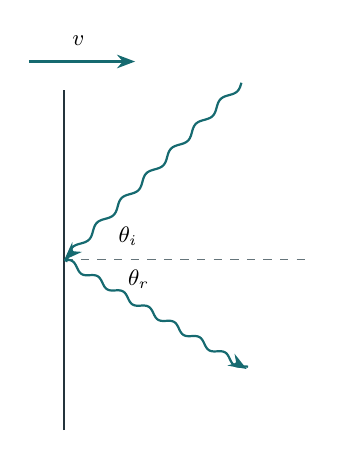
\begin{tikzpicture}[scale=.9,transform shape]
\draw[object] (0.00000,-2.40000)--(0.00000,2.40000);\draw[guide] (0.00000,0.00000)--(3.50000,0.00000);\draw[traj] plot coordinates {(2.50000,2.50000) (2.49214,2.47189) (2.48322,2.44484) (2.47231,2.41977) (2.45867,2.39744) (2.44186,2.37829) (2.42173,2.36244) (2.39853,2.34967) (2.37279,2.33944) (2.34532,2.33094) (2.31710,2.32319) (2.28920,2.31512) (2.26264,2.30571) (2.23832,2.29405) (2.21690,2.27951) (2.19872,2.26171) (2.18382,2.24064) (2.17188,2.21661) (2.16225,2.19027) (2.15408,2.16246) (2.14635,2.13423) (2.13798,2.10662) (2.12799,2.08064) (2.11554,2.05712) (2.10005,2.03664) (2.08127,2.01945) (2.05928,2.00547) (2.03449,1.99429) (2.00761,1.98519) (1.97957,1.97726) (1.95141,1.96945) (1.92419,1.96071) (1.89886,1.95006) (1.87619,1.93676) (1.85667,1.92031) (1.84046,1.90055) (1.82736,1.87767) (1.81688,1.85218) (1.80824,1.82486) (1.80045,1.79667) (1.79247,1.76868) (1.78326,1.74192) (1.77190,1.71731) (1.75770,1.69554) (1.74027,1.67700) (1.71955,1.66174) (1.69584,1.64949) (1.66971,1.63964) (1.64202,1.63136) (1.61378,1.62363) (1.58605,1.61539) (1.55985,1.60562) (1.53602,1.59348) (1.51517,1.57835) (1.49761,1.55994) (1.48329,1.53829) (1.47182,1.51379) (1.46254,1.48710) (1.45453,1.45914) (1.44676,1.43094) (1.43817,1.40356) (1.42778,1.37798) (1.41480,1.35498) (1.39872,1.33510) (1.37933,1.31851) (1.35678,1.30509) (1.33155,1.29435) (1.30438,1.28555) (1.27624,1.27772) (1.24817,1.26981) (1.22123,1.26078) (1.19634,1.24970) (1.17423,1.23585) (1.15531,1.21879) (1.13969,1.19844) (1.12713,1.17503) (1.11705,1.14914) (1.10864,1.12158) (1.10090,1.09334) (1.09277,1.06550) (1.08322,1.03908) (1.07138,1.01495) (1.05661,0.99375) (1.03857,0.97582) (1.01727,0.96114) (0.99306,0.94939) (0.96658,0.93990) (0.93871,0.93179) (0.91048,0.92405) (0.88296,0.91560) (0.85713,0.90546) (0.83382,0.89280) (0.81356,0.87708) (0.79661,0.85807) (0.78285,0.83585) (0.77184,0.81089) (0.76287,0.78390) (0.75498,0.75581) (0.74714,0.72768) (0.73828,0.70056) (0.72747,0.67541) (0.71395,0.65295) (0.69727,0.63367) (0.67728,0.61769) (0.65419,0.60480) (0.62854,0.59448) (0.60112,0.58593) (0.57291,0.57817) (0.54497,0.57014) (0.51834,0.56079) (0.49392,0.54925) (0.47237,0.53483) (0.45406,0.51716) (0.43904,0.49622) (0.42698,0.47230) (0.41728,0.44603) (0.40907,0.41827) (0.40134,0.39003) (0.39302,0.36238) (0.38311,0.33632) (0.37077,0.31269) (0.35541,0.29207) (0.33676,0.27475) (0.31489,0.26065) (0.29021,0.24936) (0.26340,0.24020) (0.23538,0.23224) (0.20721,0.22445) (0.17992,0.21576) (0.15450,0.20521) (0.13172,0.19202) (0.11207,0.17570) (0.09572,0.15608) (0.08251,0.13332) (0.07193,0.10792) (0.06323,0.08065) (0.05544,0.05248) (0.04748,0.02446) (0.03834,-0.00237) (0.02708,-0.02708)};\draw[motion] (0.12728,0.12728)--(0.00000,0.00000);\draw[traj] plot coordinates {(0.00000,0.00000) (0.02587,0.00121) (0.05098,0.00115) (0.07464,-0.00134) (0.09632,-0.00714) (0.11569,-0.01680) (0.13266,-0.03047) (0.14740,-0.04787) (0.16030,-0.06836) (0.17194,-0.09095) (0.18303,-0.11445) (0.19436,-0.13756) (0.20667,-0.15904) (0.22059,-0.17780) (0.23662,-0.19305) (0.25501,-0.20435) (0.27578,-0.21168) (0.29868,-0.21543) (0.32327,-0.21636) (0.34892,-0.21552) (0.37489,-0.21415) (0.40039,-0.21354) (0.42472,-0.21492) (0.44726,-0.21928) (0.46760,-0.22732) (0.48554,-0.23936) (0.50116,-0.25530) (0.51475,-0.27463) (0.52682,-0.29650) (0.53804,-0.31978) (0.54918,-0.34321) (0.56100,-0.36550) (0.57420,-0.38548) (0.58933,-0.40224) (0.60674,-0.41518) (0.62655,-0.42411) (0.64862,-0.42924) (0.67259,-0.43121) (0.69790,-0.43095) (0.72382,-0.42964) (0.74961,-0.42857) (0.77450,-0.42900) (0.79783,-0.43203) (0.81910,-0.43851) (0.83803,-0.44891) (0.85458,-0.46330) (0.86894,-0.48133) (0.88156,-0.50229) (0.89304,-0.52514) (0.90412,-0.54866) (0.91557,-0.57157) (0.92813,-0.59262) (0.94242,-0.61079) (0.95887,-0.62533) (0.97770,-0.63589) (0.99888,-0.64252) (1.02214,-0.64568) (1.04698,-0.64620) (1.07274,-0.64517) (1.09868,-0.64384) (1.12402,-0.64351) (1.14806,-0.64537) (1.17022,-0.65036) (1.19012,-0.65913) (1.20763,-0.67191) (1.22284,-0.68852) (1.23611,-0.70839) (1.24797,-0.73061) (1.25912,-0.75402) (1.27033,-0.77733) (1.28235,-0.79928) (1.29587,-0.81873) (1.31140,-0.83482) (1.32925,-0.84702) (1.34949,-0.85522) (1.37195,-0.85972) (1.39621,-0.86119) (1.42168,-0.86065) (1.44764,-0.85928) (1.47332,-0.85840) (1.49797,-0.85923) (1.52095,-0.86285) (1.54181,-0.87002) (1.56029,-0.88116) (1.57642,-0.89626) (1.59042,-0.91489) (1.60278,-0.93628) (1.61413,-0.95935) (1.62522,-0.98286) (1.63682,-1.00551) (1.64966,-1.02610) (1.66431,-1.04365) (1.68119,-1.05748) (1.70047,-1.06730) (1.72206,-1.07324) (1.74565,-1.07585) (1.77071,-1.07599) (1.79656,-1.07481) (1.82245,-1.07357) (1.84760,-1.07356) (1.87133,-1.07593) (1.89310,-1.08158) (1.91256,-1.09108) (1.92963,-1.10459) (1.94446,-1.12185) (1.95742,-1.14223) (1.96910,-1.16476) (1.98020,-1.18825) (1.99150,-1.21140) (2.00375,-1.23297) (2.01761,-1.25186) (2.03354,-1.26726) (2.05184,-1.27872) (2.07251,-1.28621) (2.09533,-1.29009) (2.11987,-1.29111) (2.14549,-1.29032) (2.17145,-1.28895) (2.19699,-1.28829) (2.22138,-1.28956) (2.24400,-1.29378) (2.26443,-1.30167) (2.28248,-1.31355) (2.29818,-1.32934) (2.31184,-1.34855) (2.32396,-1.37033) (2.33521,-1.39358) (2.34634,-1.41703) (2.35812,-1.43938) (2.37125,-1.45948) (2.38629,-1.47638) (2.40360,-1.48948) (2.42332,-1.49857) (2.44530,-1.50385) (2.46921,-1.50593) (2.49447,-1.50573) (2.52039,-1.50444) (2.54620,-1.50334) (2.57113,-1.50368) (2.59454,-1.50660)};\draw[motion] (2.42040,-1.44710)--(2.57489,-1.53946);\node[above] at (0.90000,0.08000) {$\theta_i$};\node[below] at (1.05000,-0.02000) {$\theta_r$};\draw[motion] (-0.50000,2.80000)--(1.00000,2.80000);\node[above] at (0.20000,2.90000) {$v$};
\end{tikzpicture}
\figcaption{图近2.4\quad 入射从右侧来，两个角从各自规定法线量起。}
\end{minipage}\end{center}

\Needspace{8\baselineskip}

\pdfbookmark[3]{题型定位}{q4-h0}

\subsection*{题型定位}

在镜面静止系使用等角、等频的理想反射定律，随后分别变换入射与反射的传播分量。实验室结果保留相遇条件、反射角象限与多普勒能量交换。图中同一入射、反射两支的角关系和频率关系都来自这两次洛伦兹变换。

\Needspace{8\baselineskip}

\pdfbookmark[3]{知识点}{q4-h1}

\subsection*{知识点}

光行差作用于传播方向，入射法向为负，镜系反射法向为正。光与镜相遇要求$\cos\theta_i+\beta>0$，反射后相对镜面分离要求$\cos\theta_r-\beta>0$。正弦关系还需余弦符号确定象限；保持两个分量可直接使用atan2。镜系频率守恒，实验室频率经入、出两次多普勒变换改变。

\Needspace{8\baselineskip}

\pdfbookmark[3]{物理图像}{q4-h2}

\subsection*{物理图像}

题图规定入射角从$-x$量、反射角从$+x$量，传播箭头各有实际方向。图A在镜静止系画等角，图B将迎面与退行镜的实验室出射线并列。图C从正的初始间隔画光线与移动镜面求交，图D画频率比随镜速改变，使几何与能量变化在同一参数下对应。

\Needspace{8\baselineskip}

\pdfbookmark[3]{解题入口}{q4-h3}

\subsection*{解题入口}

先将入射速度写为$(-c\cos\theta_i,-c\sin\theta_i)$，变到镜系，选取真正撞向镜面的负法向支。镜系反射使法向分量反号、横向保持，再变回实验室。用反射分量求角，最后由余弦差判断迎面、退行时的大小关系。

\Needspace{8\baselineskip}

\pdfbookmark[3]{标准解法}{q4-h4}

\subsection*{标准解法}


图近2.4将入射角的参考方向定为$-x$，反射角的参考方向定为$+x$。角度都由光的传播方向确定，速度变换使用朝向镜面的实际传播箭头，图中从镜面指向光源的反向线只用于几何定位。

\begin{center}\begin{minipage}{.98\linewidth}\centering
\begin{tikzpicture}[scale=.9,transform shape]
\draw[object] (0.00000,-2.00000)--(0.00000,2.00000);\draw[guide] (0.00000,0.00000)--(3.50000,0.00000);\draw[traj] plot coordinates {(2.38415,1.82094) (2.37569,1.79646) (2.36632,1.77317) (2.35524,1.75212) (2.34182,1.73413) (2.32567,1.71972) (2.30669,1.70902) (2.28506,1.70178) (2.26125,1.69740) (2.23595,1.69496) (2.21002,1.69336) (2.18435,1.69141) (2.15984,1.68794) (2.13725,1.68196) (2.11715,1.67272) (2.09984,1.65983) (2.08533,1.64326) (2.07336,1.62338) (2.06339,1.60088) (2.05466,1.57675) (2.04631,1.55212) (2.03742,1.52821) (2.02713,1.50613) (2.01472,1.48681) (1.99972,1.47090) (1.98188,1.45869) (1.96129,1.45010) (1.93830,1.44464) (1.91351,1.44153) (1.88773,1.43973) (1.86184,1.43807) (1.83676,1.43535) (1.81331,1.43050) (1.79213,1.42267) (1.77366,1.41129) (1.75803,1.39620) (1.74508,1.37760) (1.73437,1.35607) (1.72524,1.33247) (1.71684,1.30790) (1.70828,1.28356) (1.69865,1.26060) (1.68719,1.24006) (1.67329,1.22270) (1.65661,1.20897) (1.63712,1.19894) (1.61504,1.19228) (1.59091,1.18833) (1.56542,1.18613) (1.53947,1.18456) (1.51395,1.18241) (1.48974,1.17855) (1.46758,1.17202) (1.44797,1.16213) (1.43118,1.14855) (1.41717,1.13133) (1.40562,1.11091) (1.39593,1.08803) (1.38734,1.06372) (1.37896,1.03914) (1.36987,1.01548) (1.35924,0.99384) (1.34639,0.97511) (1.33087,0.95987) (1.31251,0.94835) (1.29145,0.94037) (1.26807,0.93542) (1.24304,0.93264) (1.21717,0.93095) (1.19136,0.92918) (1.16652,0.92615) (1.14345,0.92081) (1.12275,0.91235) (1.10480,0.90029) (1.08968,0.88453) (1.07718,0.86534) (1.06682,0.84335) (1.05788,0.81949) (1.04953,0.79487) (1.04083,0.77069) (1.03092,0.74811) (1.01905,0.72810) (1.00465,0.71139) (0.98746,0.69835) (0.96746,0.68897) (0.94496,0.68287) (0.92052,0.67932) (0.89488,0.67733) (0.86894,0.67574) (0.84360,0.67336) (0.81971,0.66907) (0.79799,0.66196) (0.77889,0.65141) (0.76262,0.63715) (0.74910,0.61930) (0.73794,0.59835) (0.72852,0.57513) (0.72003,0.55068) (0.71159,0.52618) (0.70228,0.50281) (0.69128,0.48165) (0.67796,0.46353) (0.66193,0.44897) (0.64305,0.43812) (0.62152,0.43076) (0.59779,0.42627) (0.57254,0.42378) (0.54661,0.42217) (0.52092,0.42025) (0.49634,0.41686) (0.47367,0.41100) (0.45345,0.40191) (0.43603,0.38917) (0.42141,0.37274) (0.40935,0.35298) (0.39931,0.33057) (0.39055,0.30648) (0.38220,0.28185) (0.37335,0.25789) (0.36313,0.23571) (0.35082,0.21627) (0.33592,0.20021) (0.31820,0.18786) (0.29772,0.17912) (0.27481,0.17355) (0.25009,0.17037) (0.22433,0.16854) (0.19842,0.16689) (0.17329,0.16424) (0.14976,0.15950) (0.12849,0.15179) (0.10990,0.14056) (0.09416,0.12562) (0.08110,0.10716) (0.07032,0.08572) (0.06113,0.06219) (0.05273,0.03764) (0.04419,0.01326) (0.03462,-0.00977) (0.02324,-0.03043)};\draw[motion] (0.14305,0.10926)--(0.00000,0.00000);\draw[traj] plot coordinates {(0.00000,0.00000) (0.02584,-0.00172) (0.05078,-0.00463) (0.07401,-0.00978) (0.09489,-0.01799) (0.11304,-0.02978) (0.12836,-0.04528) (0.14104,-0.06424) (0.15153,-0.08606) (0.16054,-0.10982) (0.16891,-0.13442) (0.17755,-0.15867) (0.18734,-0.18140) (0.19906,-0.20162) (0.21326,-0.21859) (0.23025,-0.23190) (0.25005,-0.24153) (0.27239,-0.24785) (0.29671,-0.25155) (0.32229,-0.25362) (0.34825,-0.25519) (0.37366,-0.25748) (0.39767,-0.26160) (0.41957,-0.26848) (0.43887,-0.27877) (0.45534,-0.29277) (0.46905,-0.31037) (0.48036,-0.33112) (0.48988,-0.35421) (0.49840,-0.37861) (0.50682,-0.40315) (0.51604,-0.42663) (0.52689,-0.44798) (0.54003,-0.46634) (0.55586,-0.48117) (0.57453,-0.49228) (0.59588,-0.49988) (0.61948,-0.50455) (0.64465,-0.50715) (0.67056,-0.50878) (0.69630,-0.51064) (0.72098,-0.51388) (0.74382,-0.51954) (0.76422,-0.52838) (0.78185,-0.54086) (0.79666,-0.55702) (0.80889,-0.57657) (0.81906,-0.59882) (0.82788,-0.62282) (0.83623,-0.64745) (0.84502,-0.67150) (0.85511,-0.69384) (0.86725,-0.71351) (0.88195,-0.72982) (0.89946,-0.74244) (0.91976,-0.75143) (0.94251,-0.75720) (0.96713,-0.76052) (0.99284,-0.76241) (1.01877,-0.76403) (1.04398,-0.76657) (1.06765,-0.77113) (1.08911,-0.77860) (1.10789,-0.78957) (1.12384,-0.80424) (1.13708,-0.82247) (1.14801,-0.84372) (1.15728,-0.86713) (1.16571,-0.89165) (1.17421,-0.91608) (1.18367,-0.93925) (1.19490,-0.96011) (1.20851,-0.97785) (1.22486,-0.99199) (1.24405,-1.00243) (1.26585,-1.00944) (1.28979,-1.01365) (1.31516,-1.01599) (1.34111,-1.01758) (1.36672,-1.01960) (1.39112,-1.02322) (1.41355,-1.02941) (1.43346,-1.03890) (1.45056,-1.05206) (1.46487,-1.06888) (1.47668,-1.08898) (1.48654,-1.11163) (1.49521,-1.13584) (1.50357,-1.16045) (1.51253,-1.18427) (1.52295,-1.20618) (1.53553,-1.22528) (1.55074,-1.24092) (1.56877,-1.25286) (1.58955,-1.26121) (1.61270,-1.26647) (1.63758,-1.26945) (1.66340,-1.27120) (1.68926,-1.27290) (1.71425,-1.27573) (1.73756,-1.28077) (1.75855,-1.28885) (1.77682,-1.30049) (1.79225,-1.31584) (1.80502,-1.33468) (1.81559,-1.35639) (1.82465,-1.38010) (1.83302,-1.40469) (1.84163,-1.42897) (1.85137,-1.45179) (1.86299,-1.47212) (1.87708,-1.48923) (1.89396,-1.50269) (1.91365,-1.51247) (1.93589,-1.51890) (1.96016,-1.52269) (1.98570,-1.52481) (2.01166,-1.52638) (2.03711,-1.52862) (2.06119,-1.53264) (2.08319,-1.53940) (2.10260,-1.54954) (2.11918,-1.56339) (2.13300,-1.58085) (2.14440,-1.60149) (2.15398,-1.62450) (2.16252,-1.64887) (2.17092,-1.67343) (2.18010,-1.69698) (2.19087,-1.71843) (2.20390,-1.73693) (2.21962,-1.75190) (2.23818,-1.76316) (2.25943,-1.77089) (2.28294,-1.77566) (2.30807,-1.77833) (2.33396,-1.77998) (2.35973,-1.78180) (2.38447,-1.78497) (2.40739,-1.79051)};\draw[motion] (2.24110,-1.71168)--(2.38415,-1.82094);\node[above] at (0.90000,0.08000) {$\theta_0$};\node[below] at (0.90000,-0.08000) {$\theta_0$};\node[above] at (1.50000,2.80000) {镜系：等角、同频};
\end{tikzpicture}
\figcaption{解图近2.4A\quad 先在镜面静止系使用普通反射定律。}
\end{minipage}\end{center}
解图近2.4A为镜面静止系$S'$。设入射与反射角均为$\theta_0$，镜系的反射定律为$\theta_i'=\theta_r'=\theta_0$。记$\gamma=(1-\beta^2)^{-1/2}$。由光行差公式，
\[
\frac{u_x'}c=\frac{u_x/c-\beta}{1-\beta u_x/c},
\qquad
\frac{u_y'}c=\frac{u_y/c}{\gamma(1-\beta u_x/c)}.
\]
入射光$u_x/c=-\cos\theta_i$，所以
\[
\cos\theta_0=\frac{\cos\theta_i+\beta}{1+\beta\cos\theta_i},
\qquad
\sin\theta_0=\frac{\sin\theta_i}{\gamma(1+\beta\cos\theta_i)}.
\]
入射能撞向镜面，要求镜系入射法向分量朝向镜面，即
\[
\boxed{\cos\theta_i+\beta>0}.
\]
图C以光线与镜面世界线的交点表示这个相遇条件。负$v$退行镜的速率范围由这一条件选定；超过该范围时，光与镜面的初始间隔随时间保持或增大。
\begin{center}\begin{minipage}{.98\linewidth}\centering
\begin{tikzpicture}[scale=.8,transform shape]
\draw[axis] (0,0)--(8,0) node[right] {$ct$};
\draw[axis] (0,-3)--(0,3) node[above] {$x$};
\draw[guide] (0,0)--(6,-1.8);
\draw[traj] (0,1)--(6,-2);
\draw[guide] (6,-1.8)--(6.48,-1.15) node[right] {镜面$x=-0.3ct$};
\draw[guide] (6,-2)--(6.48,-2.49) node[right] {入射$x=\ell-0.5ct$};
\node[left] at (0,1) {$\ell$};
\fill (5,-1.5) circle(.04) node[left] {相交};
\end{tikzpicture}
\figcaption{解图近2.4C\quad 示例入射60度、镜速$-0.3c$，两条世界线求交}
\end{minipage}\end{center}

反射光在镜系法向分量为$+c\cos\theta_0$。变回$S$，有
\[
\cos\theta_0=\frac{\cos\theta_r-\beta}{1-\beta\cos\theta_r},
\qquad
\sin\theta_0=\frac{\sin\theta_r}{\gamma(1-\beta\cos\theta_r)}.
\]
消去镜系角，得到两种等价关系
\[
\boxed{\frac{\cos\theta_i+\beta}{1+\beta\cos\theta_i}
=\frac{\cos\theta_r-\beta}{1-\beta\cos\theta_r}},
\]
\[
\boxed{\frac{\sin\theta_i}{1+\beta\cos\theta_i}
=\frac{\sin\theta_r}{1-\beta\cos\theta_r}}.
\]
后一式与余弦关系共同确定法向分量符号，分别选出锐角或钝角反射支。

\begin{center}\begin{minipage}{.98\linewidth}\centering
\begin{tikzpicture}[scale=.88,transform shape]
\draw[object] (0.00000,-2.80000)--(0.00000,2.80000);\draw[guide] (0.00000,0.00000)--(3.50000,0.00000);\draw[traj] plot coordinates {(2.50000,2.50000) (2.49214,2.47189) (2.48322,2.44484) (2.47231,2.41977) (2.45867,2.39744) (2.44186,2.37829) (2.42173,2.36244) (2.39853,2.34967) (2.37279,2.33944) (2.34532,2.33094) (2.31710,2.32319) (2.28920,2.31512) (2.26264,2.30571) (2.23832,2.29405) (2.21690,2.27951) (2.19872,2.26171) (2.18382,2.24064) (2.17188,2.21661) (2.16225,2.19027) (2.15408,2.16246) (2.14635,2.13423) (2.13798,2.10662) (2.12799,2.08064) (2.11554,2.05712) (2.10005,2.03664) (2.08127,2.01945) (2.05928,2.00547) (2.03449,1.99429) (2.00761,1.98519) (1.97957,1.97726) (1.95141,1.96945) (1.92419,1.96071) (1.89886,1.95006) (1.87619,1.93676) (1.85667,1.92031) (1.84046,1.90055) (1.82736,1.87767) (1.81688,1.85218) (1.80824,1.82486) (1.80045,1.79667) (1.79247,1.76868) (1.78326,1.74192) (1.77190,1.71731) (1.75770,1.69554) (1.74027,1.67700) (1.71955,1.66174) (1.69584,1.64949) (1.66971,1.63964) (1.64202,1.63136) (1.61378,1.62363) (1.58605,1.61539) (1.55985,1.60562) (1.53602,1.59348) (1.51517,1.57835) (1.49761,1.55994) (1.48329,1.53829) (1.47182,1.51379) (1.46254,1.48710) (1.45453,1.45914) (1.44676,1.43094) (1.43817,1.40356) (1.42778,1.37798) (1.41480,1.35498) (1.39872,1.33510) (1.37933,1.31851) (1.35678,1.30509) (1.33155,1.29435) (1.30438,1.28555) (1.27624,1.27772) (1.24817,1.26981) (1.22123,1.26078) (1.19634,1.24970) (1.17423,1.23585) (1.15531,1.21879) (1.13969,1.19844) (1.12713,1.17503) (1.11705,1.14914) (1.10864,1.12158) (1.10090,1.09334) (1.09277,1.06550) (1.08322,1.03908) (1.07138,1.01495) (1.05661,0.99375) (1.03857,0.97582) (1.01727,0.96114) (0.99306,0.94939) (0.96658,0.93990) (0.93871,0.93179) (0.91048,0.92405) (0.88296,0.91560) (0.85713,0.90546) (0.83382,0.89280) (0.81356,0.87708) (0.79661,0.85807) (0.78285,0.83585) (0.77184,0.81089) (0.76287,0.78390) (0.75498,0.75581) (0.74714,0.72768) (0.73828,0.70056) (0.72747,0.67541) (0.71395,0.65295) (0.69727,0.63367) (0.67728,0.61769) (0.65419,0.60480) (0.62854,0.59448) (0.60112,0.58593) (0.57291,0.57817) (0.54497,0.57014) (0.51834,0.56079) (0.49392,0.54925) (0.47237,0.53483) (0.45406,0.51716) (0.43904,0.49622) (0.42698,0.47230) (0.41728,0.44603) (0.40907,0.41827) (0.40134,0.39003) (0.39302,0.36238) (0.38311,0.33632) (0.37077,0.31269) (0.35541,0.29207) (0.33676,0.27475) (0.31489,0.26065) (0.29021,0.24936) (0.26340,0.24020) (0.23538,0.23224) (0.20721,0.22445) (0.17992,0.21576) (0.15450,0.20521) (0.13172,0.19202) (0.11207,0.17570) (0.09572,0.15608) (0.08251,0.13332) (0.07193,0.10792) (0.06323,0.08065) (0.05544,0.05248) (0.04748,0.02446) (0.03834,-0.00237) (0.02708,-0.02708)};\draw[motion] (0.12728,0.12728)--(0.00000,0.00000);\draw[motion] (0.00000,0.00000)--(2.57489,-1.53946);\node[right] at (2.57489,-1.53946) {$\beta=0.2$};\draw[force] (0.00000,0.00000)--(-0.64165,-2.93058);\node[below left] at (-0.64165,-2.93058) {$\beta=-0.5$};\node[above] at (1.70000,2.80000) {同一入射角45°};\node[below] at (1.50000,-3.50000) {退行支用相对镜面的法向速度判定};
\end{tikzpicture}
\figcaption{解图近2.4B\quad 迎光反射角变小，退行反射可进入钝角支。}
\end{minipage}\end{center}
法向、横向分量比还给出不含频率的切线形式。入射与反射在镜系的同一锐角满足$\tan\theta_0=\sin\theta_i/[\gamma(\cos\theta_i+\beta)]=\sin\theta_r/[\gamma(\cos\theta_r-\beta)]$，因此$\sin\theta_i/(\cos\theta_i+\beta)=\sin\theta_r/(\cos\theta_r-\beta)$。该式与余弦、正弦两式从同一二维速度变换导出；当反射法向分量跨零时，继续保留两个分量的符号便得到连续的钝角支。

令$D=1+\beta^2+2\beta\cos\theta_i$。解图近2.4B的实验室两条出射线按下式确定：
\[
\boxed{\cos\theta_r=\frac{(1+\beta^2)\cos\theta_i+2\beta}{D}},
\qquad
\boxed{\sin\theta_r=\frac{(1-\beta^2)\sin\theta_i}{D}}.
\]
由$D\ge(1-|\beta|)^2>0$，上述两个分量具有确定的符号。取$\theta_r=\operatorname{atan2}(\sin\theta_r,\cos\theta_r)$，正弦非负给出$0\le\theta_r\le\pi$的唯一连续方向，余弦正、零、负分别对应锐角、直角和钝角。

当$\beta=0$，立即恢复$\theta_r=\theta_i$。对允许发生碰撞的光线，
\[
\cos\theta_r-\cos\theta_i
=\frac{2\beta\sin^2\theta_i}{D}.
\]
所以非正入射时，$\beta>0$表示镜面迎着入射光运动，有$\theta_r<\theta_i$；$\beta<0$表示镜面沿入射的法向分量退行，有$\theta_r>\theta_i$。退行足够快时，反射光的实验室法向分量甚至仍为负，但它比镜面退得慢，仍然与镜面分离。判别分离应看$\cos\theta_r-\beta>0$，由光与镜面的相对法向速度判定。

同一镜系反射还给出频率与机械功的联系。两次洛伦兹变换、镜系弹性反射给
\[
\nu_i'=\gamma\nu_i(1+\beta\cos\theta_i),\qquad
\nu_r=\gamma\nu_i'(1+\beta\cos\theta_0),
\]
\[
\frac{\nu_r}{\nu_i}=\frac{D}{1-\beta^2}.
\]
图D把频率比画成镜速的函数：迎面镜反射蓝移，退行镜反射红移，分别对应光从镜面系统取得能量和向它交付能量。
\begin{center}\begin{minipage}{.98\linewidth}\centering
\begin{tikzpicture}[scale=.8,transform shape]
\draw[axis] (0,0)--(10.7,0) node[right] {$\beta$};
\draw[axis] (0,0)--(0,3.2) node[above] {$\nu_r/\nu_i$};
\node[above] at (5,3.5) {入射45度的频率比；负速率段取可碰撞支};
\draw[traj] plot coordinates {(0.000000000,0.435723969) (0.055555556,0.429538742) (0.111111111,0.423708885) (0.166666667,0.418215119) (0.222222222,0.413039660) (0.277777778,0.408166080) (0.333333333,0.403579185) (0.388888889,0.399264900) (0.444444444,0.395210173) (0.500000000,0.391402885) (0.555555556,0.387831776) (0.611111111,0.384486365) (0.666666667,0.381356894) (0.722222222,0.378434263) (0.777777778,0.375709983) (0.833333333,0.373176128) (0.888888889,0.370825289) (0.944444444,0.368650536) (1.000000000,0.366645386) (1.055555556,0.364803766) (1.111111111,0.363119985) (1.166666667,0.361588710) (1.222222222,0.360204938) (1.277777778,0.358963974) (1.333333333,0.357861412) (1.388888889,0.356893115) (1.444444444,0.356055197) (1.500000000,0.355344008) (1.555555556,0.354756120) (1.611111111,0.354288312) (1.666666667,0.353937559) (1.722222222,0.353701017) (1.777777778,0.353576019) (1.833333333,0.353560057) (1.888888889,0.353650781) (1.944444444,0.353845983) (2.000000000,0.354143596) (2.055555556,0.354541683) (2.111111111,0.355038429) (2.166666667,0.355632139) (2.222222222,0.356321230) (2.277777778,0.357104225) (2.333333333,0.357979749) (2.388888889,0.358946524) (2.444444444,0.360003366) (2.500000000,0.361149178) (2.555555556,0.362382951) (2.611111111,0.363703756) (2.666666667,0.365110744) (2.722222222,0.366603140) (2.777777778,0.368180244) (2.833333333,0.369841426) (2.888888889,0.371586124) (2.944444444,0.373413842) (3.000000000,0.375324149) (3.055555556,0.377316676) (3.111111111,0.379391114) (3.166666667,0.381547214) (3.222222222,0.383784785) (3.277777778,0.386103690) (3.333333333,0.388503850) (3.388888889,0.390985241) (3.444444444,0.393547888) (3.500000000,0.396191874) (3.555555556,0.398917329) (3.611111111,0.401724437) (3.666666667,0.404613433) (3.722222222,0.407584599) (3.777777778,0.410638271) (3.833333333,0.413774831) (3.888888889,0.416994713) (3.944444444,0.420298398) (4.000000000,0.423686419) (4.055555556,0.427159356) (4.111111111,0.430717839) (4.166666667,0.434362548) (4.222222222,0.438094213) (4.277777778,0.441913615) (4.333333333,0.445821583) (4.388888889,0.449819001) (4.444444444,0.453906802) (4.500000000,0.458085972) (4.555555556,0.462357552) (4.611111111,0.466722636) (4.666666667,0.471182371) (4.722222222,0.475737963) (4.777777778,0.480390673) (4.833333333,0.485141822) (4.888888889,0.489992789) (4.944444444,0.494945015) (5.000000000,0.500000000) (5.055555556,0.505159312) (5.111111111,0.510424582) (5.166666667,0.515797507) (5.222222222,0.521279857) (5.277777778,0.526873467) (5.333333333,0.532580250) (5.388888889,0.538402191) (5.444444444,0.544341354) (5.500000000,0.550399880) (5.555555556,0.556579997) (5.611111111,0.562884013) (5.666666667,0.569314326) (5.722222222,0.575873427) (5.777777778,0.582563898) (5.833333333,0.589388418) (5.888888889,0.596349770) (5.944444444,0.603450840) (6.000000000,0.610694621) (6.055555556,0.618084221) (6.111111111,0.625622864) (6.166666667,0.633313896) (6.222222222,0.641160790) (6.277777778,0.649167149) (6.333333333,0.657336714) (6.388888889,0.665673369) (6.444444444,0.674181147) (6.500000000,0.682864235) (6.555555556,0.691726982) (6.611111111,0.700773906) (6.666666667,0.710009703) (6.722222222,0.719439249) (6.777777778,0.729067618) (6.833333333,0.738900082) (6.888888889,0.748942125) (6.944444444,0.759199451) (7.000000000,0.769677996) (7.055555556,0.780383938) (7.111111111,0.791323711) (7.166666667,0.802504013) (7.222222222,0.813931825) (7.277777778,0.825614420) (7.333333333,0.837559382) (7.388888889,0.849774619) (7.444444444,0.862268383) (7.500000000,0.875049285) (7.555555556,0.888126315) (7.611111111,0.901508867) (7.666666667,0.915206754) (7.722222222,0.929230234) (7.777777778,0.943590039) (7.833333333,0.958297395) (7.888888889,0.973364057) (7.944444444,0.988802334) (8.000000000,1.004625126) (8.055555556,1.020845957) (8.111111111,1.037479013) (8.166666667,1.054539183) (8.222222222,1.072042102) (8.277777778,1.090004198) (8.333333333,1.108442742) (8.388888889,1.127375904) (8.444444444,1.146822809) (8.500000000,1.166803601) (8.555555556,1.187339513) (8.611111111,1.208452940) (8.666666667,1.230167516) (8.722222222,1.252508207) (8.777777778,1.275501398) (8.833333333,1.299175003) (8.888888889,1.323558567) (8.944444444,1.348683396) (9.000000000,1.374582684) (9.055555556,1.401291658) (9.111111111,1.428847737) (9.166666667,1.457290702) (9.222222222,1.486662888) (9.277777778,1.517009390) (9.333333333,1.548378291) (9.388888889,1.580820912) (9.444444444,1.614392093) (9.500000000,1.649150495) (9.555555556,1.685158939) (9.611111111,1.722484783) (9.666666667,1.761200335) (9.722222222,1.801383320) (9.777777778,1.843117392) (9.833333333,1.886492713) (9.888888889,1.931606597) (9.944444444,1.978564233) (10.000000000,2.027479494)};
\node[below] at (0,-.12) {$-0.65$};
\node[below] at (5,-.12) {$0$};
\node[below] at (10,-.12) {$0.65$};
\end{tikzpicture}
\figcaption{解图近2.4D\quad 入射45度的频率比；负速率段取可碰撞支}
\end{minipage}\end{center}给定的匀速镜速由维持机构保持，反射中的能量交换按上述频移计算。


\Needspace{8\baselineskip}

\pdfbookmark[3]{关键洞察}{q4-h5}

\subsection*{关键洞察}

反射支由光与镜面的相对法向位移确定。退行镜可以使反射光在实验室仍向左传播，而镜面向左更快，二者之间的间隔继续增大。角关系中的负法向分量与光离开镜面的条件各自有清楚定义。

\Needspace{8\baselineskip}

\pdfbookmark[3]{易错点}{q4-h6}

\subsection*{易错点}

入射两分量使用实际传播箭头，光线反向指向光源的箭头属于另一矢量。入射光行差分母为$1+\beta\cos\theta_i$，反射分母为$1-\beta\cos\theta_r$。先选能相遇的入射条件，再从余弦与正弦同时确定0至180度的出射角。实验室能量变化由运动镜面的机械功承担，镜系的弹性条件对应同一镜速维持模型。

\Needspace{8\baselineskip}

\pdfbookmark[3]{课堂讲解建议}{q4-h7}

\subsection*{课堂讲解建议}

先取镜速零确认两角参考法线，再画初始位于镜右侧的光与一条退行镜世界线。让学生用交点判断能相遇的速率范围。消元后先比较余弦差的符号，再取一个钝角反射例子，要求用光速法向分量减镜速说明光与镜面的间隔如何增长。最后用频率比解释迎面蓝移、退行红移的功交换方向。

\Needspace{8\baselineskip}

\pdfbookmark[3]{变式训练}{q4-h8}

\subsection*{变式训练}

\begin{enumerate}
\Needspace{20\baselineskip}
\item 正入射$\theta_i=0$时，求反射角与频率比；取镜速$0.5c$。
\textbf{解：}图V1中镜系与实验室的反射方向都沿$+x$，所以$\theta_r=0$。主解频率式的$D=(1+\beta)^2$，得$\nu_r/\nu_i=(1+\beta)/(1-\beta)$；0.5$c$时为3。角度保持而频率增加，光从维持迎面运动的镜面系统获得能量。该入射方向对所有$-1<\beta<1$均可追上镜面。
\begin{center}\begin{minipage}{.98\linewidth}\centering
\begin{tikzpicture}[scale=.8,transform shape]
\draw[object] (0,-1)--(0,1);\draw[force] (3,.4)--(0,.4) node[midway,above] {入射$\nu_i$};\draw[motion] (0,-.4)--(3,-.4) node[midway,below] {反射$3\nu_i$};\draw[motion] (0,1.5)--(1,1.5) node[right] {$0.5c$};
\end{tikzpicture}
\figcaption{变图近2.4V1\quad 正入射角保持，频率随镜速改变}
\end{minipage}\end{center}

\Needspace{20\baselineskip}
\item 小镜速$|\beta|\ll1$，求反射角的一阶修正并说明正入射端点。
\textbf{解：}图V2固定非零入射角，展开精确余弦得$\cos\theta_r=\cos\theta_i+2\beta\sin^2\theta_i+O(\beta^2)$。再令$\theta_r=\theta_i+\Delta\theta$，一阶为$-\sin\theta_i\Delta\theta=2\beta\sin^2\theta_i$，故$\Delta\theta=-2\beta\sin\theta_i+O(\beta^2)$，弧度制。正入射端点直接由精确式给$\theta_r=0$，与一阶修正趋零相容。
\begin{center}\begin{minipage}{.98\linewidth}\centering
\begin{tikzpicture}[scale=.8,transform shape]
\draw[axis] (0,0)--(10.7,0) node[right] {$\beta$};
\draw[axis] (0,0)--(0,3.2) node[above] {$\theta_r$（度）};
\node[above] at (5,3.5) {固定45度入射的小速度角响应};
\draw[traj] plot coordinates {(0.000000000,2.685131591) (0.083333333,2.677366594) (0.166666667,2.669619674) (0.250000000,2.661890797) (0.333333333,2.654179928) (0.416666667,2.646487033) (0.500000000,2.638812075) (0.583333333,2.631155020) (0.666666667,2.623515833) (0.750000000,2.615894478) (0.833333333,2.608290919) (0.916666667,2.600705121) (1.000000000,2.593137049) (1.083333333,2.585586666) (1.166666667,2.578053937) (1.250000000,2.570538826) (1.333333333,2.563041296) (1.416666667,2.555561313) (1.500000000,2.548098839) (1.583333333,2.540653839) (1.666666667,2.533226277) (1.750000000,2.525816115) (1.833333333,2.518423318) (1.916666667,2.511047849) (2.000000000,2.503689672) (2.083333333,2.496348750) (2.166666667,2.489025047) (2.250000000,2.481718525) (2.333333333,2.474429149) (2.416666667,2.467156881) (2.500000000,2.459901684) (2.583333333,2.452663523) (2.666666667,2.445442359) (2.750000000,2.438238156) (2.833333333,2.431050877) (2.916666667,2.423880485) (3.000000000,2.416726943) (3.083333333,2.409590213) (3.166666667,2.402470259) (3.250000000,2.395367044) (3.333333333,2.388280529) (3.416666667,2.381210679) (3.500000000,2.374157455) (3.583333333,2.367120821) (3.666666667,2.360100739) (3.750000000,2.353097172) (3.833333333,2.346110082) (3.916666667,2.339139432) (4.000000000,2.332185185) (4.083333333,2.325247303) (4.166666667,2.318325750) (4.250000000,2.311420486) (4.333333333,2.304531476) (4.416666667,2.297658681) (4.500000000,2.290802064) (4.583333333,2.283961587) (4.666666667,2.277137214) (4.750000000,2.270328906) (4.833333333,2.263536626) (4.916666667,2.256760336) (5.000000000,2.250000000) (5.083333333,2.243255579) (5.166666667,2.236527036) (5.250000000,2.229814334) (5.333333333,2.223117434) (5.416666667,2.216436300) (5.500000000,2.209770894) (5.583333333,2.203121179) (5.666666667,2.196487116) (5.750000000,2.189868669) (5.833333333,2.183265800) (5.916666667,2.176678471) (6.000000000,2.170106646) (6.083333333,2.163550286) (6.166666667,2.157009355) (6.250000000,2.150483814) (6.333333333,2.143973627) (6.416666667,2.137478756) (6.500000000,2.130999164) (6.583333333,2.124534813) (6.666666667,2.118085666) (6.750000000,2.111651686) (6.833333333,2.105232836) (6.916666667,2.098829077) (7.000000000,2.092440374) (7.083333333,2.086066689) (7.166666667,2.079707984) (7.250000000,2.073364223) (7.333333333,2.067035369) (7.416666667,2.060721384) (7.500000000,2.054422231) (7.583333333,2.048137873) (7.666666667,2.041868274) (7.750000000,2.035613395) (7.833333333,2.029373202) (7.916666667,2.023147655) (8.000000000,2.016936720) (8.083333333,2.010740358) (8.166666667,2.004558533) (8.250000000,1.998391208) (8.333333333,1.992238347) (8.416666667,1.986099912) (8.500000000,1.979975868) (8.583333333,1.973866177) (8.666666667,1.967770804) (8.750000000,1.961689710) (8.833333333,1.955622861) (8.916666667,1.949570220) (9.000000000,1.943531750) (9.083333333,1.937507414) (9.166666667,1.931497177) (9.250000000,1.925501003) (9.333333333,1.919518854) (9.416666667,1.913550696) (9.500000000,1.907596491) (9.583333333,1.901656205) (9.666666667,1.895729800) (9.750000000,1.889817240) (9.833333333,1.883918491) (9.916666667,1.878033516) (10.000000000,1.872162278)};
\node[below] at (0,-.12) {$-0.1$};
\node[below] at (5,-.12) {$0$};
\node[below] at (10,-.12) {$0.1$};
\end{tikzpicture}
\figcaption{变图近2.4V2\quad 固定45度入射的小速度角响应}
\end{minipage}\end{center}

\Needspace{20\baselineskip}
\item 入射角60度，求使反射光在实验室恰沿镜面切向的镜速。
\textbf{解：}图V3要求$\cos\theta_r=0$，故$(1+\beta^2)/2+2\beta=0$，即$\beta^2+4\beta+1=0$。允许根为$\beta=-2+\sqrt3$，另一根小于−1。相遇因子为$1/2+\beta=\sqrt3-3/2>0$，因此确可发生。反射光的实验室法向速度为零，镜面仍向左退，二者继续分离。
\begin{center}\begin{minipage}{.98\linewidth}\centering
\begin{tikzpicture}[scale=.8,transform shape]
\draw[axis] (-2.5,0)--(2.7,0) node[right] {$x$};
\draw[axis] (0,-2.5)--(0,2.7) node[above] {$y$};
\draw[traj] (-0.000000000,-2.200000000)--(0.000000000,2.200000000);
\node[above] at (0.000000000,2.350000000) {反射切向};
\draw[guide] (-1.800000000,-0.000000000)--(1.800000000,0.000000000);
\node[above] at (1.800000000,0.150000000) {法线};
\end{tikzpicture}
\figcaption{变图近2.4V3\quad 入射60度时镜速$(-2+\sqrt3)c$}
\end{minipage}\end{center}

\Needspace{20\baselineskip}
\item 镜速为$-0.5c$、入射角45度，证明反射光在实验室仍有负法向速度而能离开镜面。
\textbf{解：}图V4中$D=5/4-1/\sqrt2>0$，$\cos\theta_r=[5/(4\sqrt2)-1]/D<0$，$\sin\theta_r=[3/(4\sqrt2)]/D>0$，因此取二象限角。将余弦与镜速比较，$\cos\theta_r+1/2>0$。光的负法向速度绝对值小于镜面退行速率，镜面更快向左离开，反射光留在其右侧且法向间隔随反射后的时间线性增长。
\begin{center}\begin{minipage}{.98\linewidth}\centering
\begin{tikzpicture}[scale=.8,transform shape]
\draw[axis] (-2.5,0)--(2.7,0) node[right] {$x$};
\draw[axis] (0,-2.5)--(0,2.7) node[above] {$y$};
\draw[traj] (0.470546220,-2.149089634)--(-0.470546220,2.149089634);
\node[above] at (-0.470546220,2.299089634) {钝角反射支};
\end{tikzpicture}
\figcaption{变图近2.4V4\quad 退行$-0.5c$、入射45度，反射法向仍为负}
\end{minipage}\end{center}

\Needspace{20\baselineskip}
\item 由光的能量与法向动量说明频率比怎样体现镜面机械功。
\textbf{解：}图V5以入射光子能量为1、$c=1$归一化。运动镜面保持的组合为$\omega-vk_x$，镜系频率相同给$\nu_i(1+\beta\cos\theta_i)=\nu_r(1-\beta\cos\theta_r)$。因此频率比也等于$(1+\beta\cos\theta_i)/(1-\beta\cos\theta_r)$。光子动量差传给镜面，$\Delta E_m=1-\nu_r/\nu_i$、$\Delta p_{mx}=-\cos\theta_i-(\nu_r/\nu_i)\cos\theta_r$，满足$\Delta E_m=\beta\Delta p_{mx}$。迎面镜给光做正功，退行镜从光取得能量。
\begin{center}\begin{minipage}{.98\linewidth}\centering
\begin{tikzpicture}[scale=.8,transform shape]
\node at (0,1) {光子能量变化};\node at (6,1) {镜面能量变化};\node at (0,0) {$h(\nu_r-\nu_i)$};\node at (6,0) {$v\Delta p_{mx}$};\node at (3,-1) {$h(\nu_i-\nu_r)=v\Delta p_{mx}$};
\end{tikzpicture}
\figcaption{变图近2.4V5\quad 镜速维持时，光与镜面的功、动量交换相配}
\end{minipage}\end{center}

\Needspace{20\baselineskip}
\item 正入射时测得反射频率为入射3倍，反求镜速并求光给镜面的法向动量。
\textbf{解：}图V6由$R=(1+\beta)/(1-\beta)$解得$\beta=(R-1)/(R+1)=1/2$。入射光子动量沿$-x$为$-h\nu_i/c$，反射沿$+x$为$3h\nu_i/c$，镜面得到$-4h\nu_i/c$。相应能量变化为$v\Delta p=-2h\nu_i$，光子的能量增加$2h\nu_i$；维持镜速的机构向该过程供能。
\begin{center}\begin{minipage}{.98\linewidth}\centering
\begin{tikzpicture}[scale=.8,transform shape]
\draw[axis] (0,0)--(10.7,0);
\draw[axis] (0,0)--(0,3.2);
\draw[line width=7pt,color=accent] (1.0,0)--(1.0,0.900000000);
\node[below] at (1.0,-.14) {入射能量};
\node[above] at (1.0,1.040000000) {$ 1 $};
\draw[line width=7pt,color=accent] (5.0,0)--(5.0,2.700000000);
\node[below] at (5.0,-.14) {反射能量};
\node[above] at (5.0,2.840000000) {$ 3 $};
\draw[line width=7pt,color=accent] (9.0,0)--(9.0,1.800000000);
\node[below] at (9.0,-.14) {镜面供给能量};
\node[above] at (9.0,1.940000000) {$ 2 $};
\end{tikzpicture}
\figcaption{变图近2.4V6\quad 以$h\nu_i$为单位；迎面$0.5c$镜面供能}
\end{minipage}\end{center}

\Needspace{20\baselineskip}
\item 入射光最初位于镜面右侧法向距离$\ell$处，求碰撞时间并讨论退行临界速率。
\textbf{解：}图V7中光线$x=\ell-c\cos\theta_i t$，镜面$x=\beta ct$，相交给$t_h=\ell/[c(\cos\theta_i+\beta)]$。正的有限碰撞时间要求分母为正。对非正入射，当$\beta\to-\cos\theta_i$的允许一侧时，时间趋于无穷大，光与镜面法向速率趋同。该极限的反射公式趋向原传播方向、频率比趋1；临界等速下初始间隔保持，实际碰撞尚未发生。
\begin{center}\begin{minipage}{.98\linewidth}\centering
\begin{tikzpicture}[scale=.8,transform shape]
\draw[axis] (0,0)--(10.7,0) node[right] {$\beta$};
\draw[axis] (0,0)--(0,3.2) node[above] {$ct_h/\ell$};
\node[above] at (5,3.5) {退行速率趋向相遇临界值时碰撞时间增长};
\draw[traj] plot coordinates {(0.000000000,2.626658286) (0.083333333,2.336808419) (0.166666667,2.104570559) (0.250000000,1.914320595) (0.333333333,1.755615624) (0.416666667,1.621210660) (0.500000000,1.505921567) (0.583333333,1.405940941) (0.666666667,1.318409548) (0.750000000,1.241138466) (0.833333333,1.172423525) (0.916666667,1.110918158) (1.000000000,1.055544280) (1.083333333,1.005428547) (1.166666667,0.959855958) (1.250000000,0.918235527) (1.333333333,0.880074508) (1.416666667,0.844958803) (1.500000000,0.812537866) (1.583333333,0.782512966) (1.666666667,0.754627953) (1.750000000,0.728661933) (1.833333333,0.704423403) (1.916666667,0.681745521) (2.000000000,0.660482260) (2.083333333,0.640505259) (2.166666667,0.621701233) (2.250000000,0.603969818) (2.333333333,0.587221785) (2.416666667,0.571377533) (2.500000000,0.556365828) (2.583333333,0.542122729) (2.666666667,0.528590681) (2.750000000,0.515717734) (2.833333333,0.503456878) (2.916666667,0.491765473) (3.000000000,0.480604745) (3.083333333,0.469939366) (3.166666667,0.459737073) (3.250000000,0.449968348) (3.333333333,0.440606126) (3.416666667,0.431625552) (3.500000000,0.423003755) (3.583333333,0.414719656) (3.666666667,0.406753797) (3.750000000,0.399088183) (3.833333333,0.391706155) (3.916666667,0.384592262) (4.000000000,0.377732154) (4.083333333,0.371112490) (4.166666667,0.364720846) (4.250000000,0.358545640) (4.333333333,0.352576062) (4.416666667,0.346802007) (4.500000000,0.341214027) (4.583333333,0.335803267) (4.666666667,0.330561430) (4.750000000,0.325480727) (4.833333333,0.320553839) (4.916666667,0.315773886) (5.000000000,0.311134391) (5.083333333,0.306629254) (5.166666667,0.302252721) (5.250000000,0.297999363) (5.333333333,0.293864051) (5.416666667,0.289841940) (5.500000000,0.285928443) (5.583333333,0.282119219) (5.666666667,0.278410157) (5.750000000,0.274797356) (5.833333333,0.271277117) (5.916666667,0.267845928) (6.000000000,0.264500452) (6.083333333,0.261237517) (6.166666667,0.258054106) (6.250000000,0.254947346) (6.333333333,0.251914502) (6.416666667,0.248952967) (6.500000000,0.246060255) (6.583333333,0.243233995) (6.666666667,0.240471922) (6.750000000,0.237771875) (6.833333333,0.235131788) (6.916666667,0.232549686) (7.000000000,0.230023678) (7.083333333,0.227551956) (7.166666667,0.225132790) (7.250000000,0.222764520) (7.333333333,0.220445557) (7.416666667,0.218174377) (7.500000000,0.215949519) (7.583333333,0.213769578) (7.666666667,0.211633210) (7.750000000,0.209539120) (7.833333333,0.207486066) (7.916666667,0.205472852) (8.000000000,0.203498331) (8.083333333,0.201561398) (8.166666667,0.199660990) (8.250000000,0.197796082) (8.333333333,0.195965690) (8.416666667,0.194168864) (8.500000000,0.192404689) (8.583333333,0.190672283) (8.666666667,0.188970796) (8.750000000,0.187299407) (8.833333333,0.185657324) (8.916666667,0.184043785) (9.000000000,0.182458050) (9.083333333,0.180899407) (9.166666667,0.179367168) (9.250000000,0.177860667) (9.333333333,0.176379262) (9.416666667,0.174922331) (9.500000000,0.173489271) (9.583333333,0.172079501) (9.666666667,0.170692458) (9.750000000,0.169327597) (9.833333333,0.167984390) (9.916666667,0.166662325) (10.000000000,0.165360907)};
\node[below] at (0,-.12) {$-0.65$};
\node[below] at (10,-.12) {$0.2$};
\end{tikzpicture}
\figcaption{变图近2.4V7\quad 退行速率趋向相遇临界值时碰撞时间增长}
\end{minipage}\end{center}

\Needspace{20\baselineskip}
\item 证明反射后光与镜面的分离速率为正，并取$\theta_i=60^\circ,\beta=-0.3$计算10纳秒后的法向间隔。
\textbf{解：}图V8从精确余弦减去$\beta$，得$\cos\theta_r-\beta=(1-\beta^2)(\cos\theta_i+\beta)/D$。允许碰撞时右端为正，所以反射后间隔$\Delta x=c(\cos\theta_r-\beta)\Delta t$增长。给定数值下$D=0.79$，$\cos\theta_r=-11/158$而分离因子为$91/395$。10纳秒对应$c\Delta t=3$米，故间隔$273/395$米，约0.69114米。光和镜面在实验室均向左，镜面退行更快。
\begin{center}\begin{minipage}{.98\linewidth}\centering
\begin{tikzpicture}[scale=.8,transform shape]
\draw[axis] (0,0)--(10.7,0) node[right] {反射后时间（纳秒）};
\draw[axis] (0,0)--(0,3.2) node[above] {法向间隔（米）};
\node[above] at (5,3.5) {入射60度、镜速$-0.3c$的间隔增长};
\draw[traj] plot coordinates {(0.000000000,0.000000000) (0.100000000,0.027645570) (0.200000000,0.055291139) (0.300000000,0.082936709) (0.400000000,0.110582278) (0.500000000,0.138227848) (0.600000000,0.165873418) (0.700000000,0.193518987) (0.800000000,0.221164557) (0.900000000,0.248810127) (1.000000000,0.276455696) (1.100000000,0.304101266) (1.200000000,0.331746835) (1.300000000,0.359392405) (1.400000000,0.387037975) (1.500000000,0.414683544) (1.600000000,0.442329114) (1.700000000,0.469974684) (1.800000000,0.497620253) (1.900000000,0.525265823) (2.000000000,0.552911392) (2.100000000,0.580556962) (2.200000000,0.608202532) (2.300000000,0.635848101) (2.400000000,0.663493671) (2.500000000,0.691139241) (2.600000000,0.718784810) (2.700000000,0.746430380) (2.800000000,0.774075949) (2.900000000,0.801721519) (3.000000000,0.829367089) (3.100000000,0.857012658) (3.200000000,0.884658228) (3.300000000,0.912303797) (3.400000000,0.939949367) (3.500000000,0.967594937) (3.600000000,0.995240506) (3.700000000,1.022886076) (3.800000000,1.050531646) (3.900000000,1.078177215) (4.000000000,1.105822785) (4.100000000,1.133468354) (4.200000000,1.161113924) (4.300000000,1.188759494) (4.400000000,1.216405063) (4.500000000,1.244050633) (4.600000000,1.271696203) (4.700000000,1.299341772) (4.800000000,1.326987342) (4.900000000,1.354632911) (5.000000000,1.382278481) (5.100000000,1.409924051) (5.200000000,1.437569620) (5.300000000,1.465215190) (5.400000000,1.492860759) (5.500000000,1.520506329) (5.600000000,1.548151899) (5.700000000,1.575797468) (5.800000000,1.603443038) (5.900000000,1.631088608) (6.000000000,1.658734177) (6.100000000,1.686379747) (6.200000000,1.714025316) (6.300000000,1.741670886) (6.400000000,1.769316456) (6.500000000,1.796962025) (6.600000000,1.824607595) (6.700000000,1.852253165) (6.800000000,1.879898734) (6.900000000,1.907544304) (7.000000000,1.935189873) (7.100000000,1.962835443) (7.200000000,1.990481013) (7.300000000,2.018126582) (7.400000000,2.045772152) (7.500000000,2.073417722) (7.600000000,2.101063291) (7.700000000,2.128708861) (7.800000000,2.156354430) (7.900000000,2.184000000) (8.000000000,2.211645570) (8.100000000,2.239291139) (8.200000000,2.266936709) (8.300000000,2.294582278) (8.400000000,2.322227848) (8.500000000,2.349873418) (8.600000000,2.377518987) (8.700000000,2.405164557) (8.800000000,2.432810127) (8.900000000,2.460455696) (9.000000000,2.488101266) (9.100000000,2.515746835) (9.200000000,2.543392405) (9.300000000,2.571037975) (9.400000000,2.598683544) (9.500000000,2.626329114) (9.600000000,2.653974684) (9.700000000,2.681620253) (9.800000000,2.709265823) (9.900000000,2.736911392) (10.000000000,2.764556962)};
\node[below] at (0,-.12) {$0$};
\node[below] at (5,-.12) {$5$};
\node[below] at (10,-.12) {$10$};
\end{tikzpicture}
\figcaption{变图近2.4V8\quad 入射60度、镜速$-0.3c$的间隔增长}
\end{minipage}\end{center}
\end{enumerate}

\Needspace{13\baselineskip}

\pdfbookmark[2]{第 5 题 共同运动的介质界面}{q5}

\section*{第 5 题\quad 共同运动的介质界面}\label{q:5}

两种均匀、透明、各向同性且无色散的介质与它们的平面界面共同以$v=\beta c$沿实验室系$S$的$+x$运动，$0\le\beta<1$，界面法线为$x$轴。两介质在共同静止系$S'$的折射率为$n_1,n_2\ge1$。光从介质1射向介质2；在$S$中，入射角$\theta_i$从$+x$量起，反射角$\theta_r$从$-x$量起，折射角$\theta_t$从$+x$量起，均取图示正横向分量。

求实验室中反射角、折射角与入射角的关系，说明传播分支与适用角域；再给出介质1为真空、介质2折射率为$n$时的结果。只讨论能射到界面的入射支；若发生全反射，应指出没有传播折射光。

\begin{center}\begin{minipage}{.98\linewidth}\centering
\begin{tikzpicture}[scale=.9,transform shape]
\draw[object] (0.00000,-2.80000)--(0.00000,2.80000);\draw[guide] (-3.20000,0.00000)--(3.80000,0.00000);\draw[traj] plot coordinates {(-2.38415,-1.82094) (-2.37569,-1.79646) (-2.36632,-1.77317) (-2.35524,-1.75212) (-2.34182,-1.73413) (-2.32567,-1.71972) (-2.30669,-1.70902) (-2.28506,-1.70178) (-2.26125,-1.69740) (-2.23595,-1.69496) (-2.21002,-1.69336) (-2.18435,-1.69141) (-2.15984,-1.68794) (-2.13725,-1.68196) (-2.11715,-1.67272) (-2.09984,-1.65983) (-2.08533,-1.64326) (-2.07336,-1.62338) (-2.06339,-1.60088) (-2.05466,-1.57675) (-2.04631,-1.55212) (-2.03742,-1.52821) (-2.02713,-1.50613) (-2.01472,-1.48681) (-1.99972,-1.47090) (-1.98188,-1.45869) (-1.96129,-1.45010) (-1.93830,-1.44464) (-1.91351,-1.44153) (-1.88773,-1.43973) (-1.86184,-1.43807) (-1.83676,-1.43535) (-1.81331,-1.43050) (-1.79213,-1.42267) (-1.77366,-1.41129) (-1.75803,-1.39620) (-1.74508,-1.37760) (-1.73437,-1.35607) (-1.72524,-1.33247) (-1.71684,-1.30790) (-1.70828,-1.28356) (-1.69865,-1.26060) (-1.68719,-1.24006) (-1.67329,-1.22270) (-1.65661,-1.20897) (-1.63712,-1.19894) (-1.61504,-1.19228) (-1.59091,-1.18833) (-1.56542,-1.18613) (-1.53947,-1.18456) (-1.51395,-1.18241) (-1.48974,-1.17855) (-1.46758,-1.17202) (-1.44797,-1.16213) (-1.43118,-1.14855) (-1.41717,-1.13133) (-1.40562,-1.11091) (-1.39593,-1.08803) (-1.38734,-1.06372) (-1.37896,-1.03914) (-1.36987,-1.01548) (-1.35924,-0.99384) (-1.34639,-0.97511) (-1.33087,-0.95987) (-1.31251,-0.94835) (-1.29145,-0.94037) (-1.26807,-0.93542) (-1.24304,-0.93264) (-1.21717,-0.93095) (-1.19136,-0.92918) (-1.16652,-0.92615) (-1.14345,-0.92081) (-1.12275,-0.91235) (-1.10480,-0.90029) (-1.08968,-0.88453) (-1.07718,-0.86534) (-1.06682,-0.84335) (-1.05788,-0.81949) (-1.04953,-0.79487) (-1.04083,-0.77069) (-1.03092,-0.74811) (-1.01905,-0.72810) (-1.00465,-0.71139) (-0.98746,-0.69835) (-0.96746,-0.68897) (-0.94496,-0.68287) (-0.92052,-0.67932) (-0.89488,-0.67733) (-0.86894,-0.67574) (-0.84360,-0.67336) (-0.81971,-0.66907) (-0.79799,-0.66196) (-0.77889,-0.65141) (-0.76262,-0.63715) (-0.74910,-0.61930) (-0.73794,-0.59835) (-0.72852,-0.57513) (-0.72003,-0.55068) (-0.71159,-0.52618) (-0.70228,-0.50281) (-0.69128,-0.48165) (-0.67796,-0.46353) (-0.66193,-0.44897) (-0.64305,-0.43812) (-0.62152,-0.43076) (-0.59779,-0.42627) (-0.57254,-0.42378) (-0.54661,-0.42217) (-0.52092,-0.42025) (-0.49634,-0.41686) (-0.47367,-0.41100) (-0.45345,-0.40191) (-0.43603,-0.38917) (-0.42141,-0.37274) (-0.40935,-0.35298) (-0.39931,-0.33057) (-0.39055,-0.30648) (-0.38220,-0.28185) (-0.37335,-0.25789) (-0.36313,-0.23571) (-0.35082,-0.21627) (-0.33592,-0.20021) (-0.31820,-0.18786) (-0.29772,-0.17912) (-0.27481,-0.17355) (-0.25009,-0.17037) (-0.22433,-0.16854) (-0.19842,-0.16689) (-0.17329,-0.16424) (-0.14976,-0.15950) (-0.12849,-0.15179) (-0.10990,-0.14056) (-0.09416,-0.12562) (-0.08110,-0.10716) (-0.07032,-0.08572) (-0.06113,-0.06219) (-0.05273,-0.03764) (-0.04419,-0.01326) (-0.03462,0.00977) (-0.02324,0.03043)};\draw[motion] (-0.14305,-0.10926)--(0.00000,0.00000);\draw[traj] plot coordinates {(0.00000,0.00000) (-0.02430,0.00896) (-0.04740,0.01880) (-0.06822,0.03031) (-0.08593,0.04409) (-0.10001,0.06053) (-0.11032,0.07973) (-0.11711,0.10150) (-0.12101,0.12540) (-0.12293,0.15074) (-0.12400,0.17670) (-0.12543,0.20240) (-0.12840,0.22698) (-0.13392,0.24968) (-0.14274,0.26997) (-0.15528,0.28754) (-0.17154,0.30238) (-0.19118,0.31476) (-0.21347,0.32519) (-0.23742,0.33440) (-0.26187,0.34326) (-0.28559,0.35264) (-0.30746,0.36337) (-0.32653,0.37617) (-0.34212,0.39150) (-0.35396,0.40958) (-0.36214,0.43034) (-0.36712,0.45344) (-0.36972,0.47828) (-0.37100,0.50410) (-0.37213,0.53001) (-0.37434,0.55515) (-0.37871,0.57869) (-0.38611,0.60002) (-0.39711,0.61872) (-0.41187,0.63466) (-0.43020,0.64799) (-0.45152,0.65913) (-0.47492,0.66875) (-0.49931,0.67764) (-0.52348,0.68670) (-0.54624,0.69679) (-0.56654,0.70867) (-0.58361,0.72293) (-0.59699,0.73988) (-0.60663,0.75957) (-0.61283,0.78178) (-0.61629,0.80599) (-0.61797,0.83151) (-0.61901,0.85749) (-0.62064,0.88305) (-0.62400,0.90733) (-0.63008,0.92963) (-0.63957,0.94943) (-0.65280,0.96649) (-0.66973,0.98085) (-0.68992,0.99282) (-0.71259,1.00297) (-0.73672,1.01205) (-0.76113,1.02094) (-0.78460,1.03050) (-0.80601,1.04158) (-0.82448,1.05481) (-0.83940,1.07063) (-0.85054,1.08922) (-0.85808,1.11045) (-0.86256,1.13392) (-0.86483,1.15900) (-0.86599,1.18490) (-0.86723,1.21074) (-0.86976,1.23564) (-0.87463,1.25882) (-0.88266,1.27968) (-0.89435,1.29788) (-0.90980,1.31331) (-0.92873,1.32620) (-0.95050,1.33701) (-0.97418,1.34643) (-0.99862,1.35529) (-1.02261,1.36447) (-1.04499,1.37484) (-1.06475,1.38712) (-1.08116,1.40185) (-1.09385,1.41931) (-1.10282,1.43950) (-1.10846,1.46212) (-1.11151,1.48663) (-1.11298,1.51230) (-1.11404,1.53827) (-1.11590,1.56365) (-1.11970,1.58762) (-1.12637,1.60949) (-1.13653,1.62880) (-1.15045,1.64535) (-1.16802,1.65924) (-1.18874,1.67082) (-1.21176,1.68071) (-1.23604,1.68969) (-1.26036,1.69864) (-1.28353,1.70842) (-1.30446,1.71985) (-1.32231,1.73353) (-1.33654,1.74986) (-1.34700,1.76895) (-1.35392,1.79063) (-1.35792,1.81445) (-1.35990,1.83975) (-1.36098,1.86570) (-1.36237,1.89143) (-1.36526,1.91607) (-1.37066,1.93886) (-1.37934,1.95925) (-1.39172,1.97694) (-1.40784,1.99188) (-1.42736,2.00435) (-1.44956,2.01484) (-1.47346,2.02409) (-1.49791,2.03294) (-1.52169,2.04228) (-1.54365,2.05295) (-1.56284,2.06566) (-1.57859,2.08088) (-1.59058,2.09885) (-1.59890,2.11951) (-1.60400,2.14252) (-1.60668,2.16731) (-1.60798,2.19310) (-1.60910,2.21903) (-1.61124,2.24421) (-1.61550,2.26783) (-1.62277,2.28926) (-1.63361,2.30807) (-1.64823,2.32411) (-1.66643,2.33754) (-1.68763,2.34877) (-1.71098,2.35843) (-1.73535,2.36733) (-1.75955,2.37637) (-1.78238,2.38640) (-1.80280,2.39820)};\draw[motion] (-1.66559,2.27557)--(-1.77191,2.42082);\draw[traj] plot coordinates {(0.00000,0.00000) (0.01489,0.02119) (0.03032,0.04099) (0.04678,0.05817) (0.06465,0.07175) (0.08415,0.08114) (0.10535,0.08619) (0.12814,0.08717) (0.15223,0.08481) (0.17722,0.08017) (0.20259,0.07455) (0.22780,0.06934) (0.25231,0.06591) (0.27567,0.06542) (0.29755,0.06874) (0.31774,0.07636) (0.33626,0.08828) (0.35325,0.10408) (0.36905,0.12295) (0.38410,0.14374) (0.39893,0.16510) (0.41408,0.18563) (0.43006,0.20401) (0.44732,0.21916) (0.46613,0.23030) (0.48665,0.23711) (0.50881,0.23969) (0.53241,0.23858) (0.55709,0.23473) (0.58237,0.22934) (0.60771,0.22379) (0.63257,0.21948) (0.65645,0.21766) (0.67896,0.21935) (0.69986,0.22519) (0.71905,0.23537) (0.73663,0.24967) (0.75287,0.26742) (0.76816,0.28757) (0.78301,0.30887) (0.79797,0.32990) (0.81355,0.34931) (0.83025,0.36589) (0.84840,0.37873) (0.86822,0.38732) (0.88972,0.39159) (0.91278,0.39189) (0.93707,0.38902) (0.96216,0.38410) (0.98755,0.37845) (1.01266,0.37347) (1.03700,0.37049) (1.06011,0.37065) (1.08168,0.37475) (1.10157,0.38316) (1.11978,0.39584) (1.13653,0.41228) (1.15215,0.43160) (1.16712,0.45259) (1.18196,0.47391) (1.19723,0.49414) (1.21342,0.51200) (1.23095,0.52645) (1.25007,0.53681) (1.27089,0.54282) (1.29334,0.54467) (1.31718,0.54298) (1.34200,0.53874) (1.36734,0.53322) (1.39263,0.52779) (1.41734,0.52385) (1.44100,0.52262) (1.46322,0.52503) (1.48380,0.53166) (1.50269,0.54264) (1.52000,0.55763) (1.53603,0.57591) (1.55120,0.59637) (1.56603,0.61773) (1.58106,0.63856) (1.59682,0.65753) (1.61376,0.67348) (1.63221,0.68557) (1.65234,0.69336) (1.67414,0.69685) (1.69745,0.69650) (1.72193,0.69317) (1.74712,0.68800) (1.77249,0.68237) (1.79750,0.67766) (1.82164,0.67519) (1.84449,0.67602) (1.86576,0.68089) (1.88533,0.69011) (1.90326,0.70353) (1.91977,0.72058) (1.93523,0.74030) (1.95013,0.76146) (1.96502,0.78268) (1.98042,0.80256) (1.99683,0.81987) (2.01463,0.83361) (2.03406,0.84317) (2.05520,0.84839) (2.07793,0.84953) (2.10197,0.84728) (2.12693,0.84271) (2.15230,0.83710) (2.17752,0.83185) (2.20207,0.82832) (2.22549,0.82769) (2.24743,0.83085) (2.26769,0.83829) (2.28627,0.85004) (2.30333,0.86570) (2.31916,0.88447) (2.33423,0.90520) (2.34906,0.92657) (2.36418,0.94716) (2.38013,0.96565) (2.39732,0.98094) (2.41607,0.99226) (2.43652,0.99924) (2.45862,1.00198) (2.48217,1.00101) (2.50681,0.99725) (2.53208,0.99189) (2.55743,0.98632) (2.58231,0.98193) (2.60624,0.98000) (2.62882,0.98153) (2.64978,0.98719) (2.66904,0.99720) (2.68668,1.01135) (2.70297,1.02897) (2.71829,1.04905) (2.73315,1.07033) (2.74809,1.09140) (2.76364,1.11090) (2.78028,1.12761)};\draw[motion] (2.62656,1.02643)--(2.79422,1.09195);\node[above] at (-2.00000,2.80000) {介质1};\node[above] at (2.00000,2.80000) {介质2};\node[below] at (-1.10000,-0.04000) {$\theta_i$};\node[above] at (-1.05000,0.06000) {$\theta_r$};\node[below] at (1.65000,-0.04000) {$\theta_t$};\draw[motion] (-0.50000,3.50000)--(1.00000,3.50000);\node[above] at (0.25000,3.60000) {$v$};
\end{tikzpicture}
\figcaption{图近2.5\quad 界面和两介质共同移动，三角均按传播方向定义。}
\end{minipage}\end{center}

\Needspace{8\baselineskip}

\pdfbookmark[3]{题型定位}{q5-h0}

\subsection*{题型定位}

介质与界面有共同静止系，在该系先建立普通反射、折射关系，再变换三支光线的传播速度。以静止系入射角为中间参数，可同时给出实验室角关系和能到达界面的入射范围。反射象限、临界折射和无相遇分别由相遇事件和静止系的各传播根确定。

\Needspace{8\baselineskip}

\pdfbookmark[3]{知识点}{q5-h1}

\subsection*{知识点}

折射率在介质静止系定义，无色散条件使该系光线速度为$c/n_j$。速度相加同时改变纵、横分量，取比后才得到角关系。入射支满足$\cos\psi>0$，透射支满足$n_1\sin\psi\le n_2$；等号对应沿界面切向的临界极限。实验室反射方向用两个分量确定，允许从$-x$量起的角跨越90度。

\Needspace{8\baselineskip}

\pdfbookmark[3]{物理图像}{q5-h2}

\subsection*{物理图像}

图A在界面静止系标入射、反射与折射的法向正负，图C列三支速度分量的共同变换结构。图B以真空入射、$n=1.5$画三种运动速率的角响应，各曲线在能追上界面的角域内结束。图D区分入射角域端点与全反射临界角，前者对应无有限相遇，后者对应已到界面的光只剩反射传播。

\Needspace{8\baselineskip}

\pdfbookmark[3]{解题入口}{q5-h3}

\subsection*{解题入口}

先以$\psi$给出静止系三条光线，再计算实验室$\theta_i(\psi)$，由其单调性选定正根和允许范围。静止系反射支把法向分量反号，折射支用Snell关系选$\cos\psi_t\ge0$的传播根，分别变回实验室。真空入射时用光行差逆式将$\psi$消去，最后以$v=0$读出静止界面定律。

\Needspace{8\baselineskip}

\pdfbookmark[3]{标准解法}{q5-h4}

\subsection*{标准解法}


图近2.5中，折射率是在介质静止系定义的。运动介质中的实验室光速由静止介质光速$c/n_j$作速度变换得到。记$\gamma=(1-\beta^2)^{-1/2}$，静止界面系入射角为$\psi$，则
\[
0\le\psi<\frac\pi2,\qquad
\theta_r'=\psi,\qquad n_1\sin\psi=n_2\sin\psi_t.
\]
解图近2.5A先在$S'$作普通反射、折射，再将三支传播速度分别变回$S$。两种介质在 $S'$ 中均匀、各向同性且无色散。这个系里群速度与相速度同向，光线的传播速率为 $c/n_j$。实验室图跟踪光线到达界面后的方向，因此对群速度的两个分量作变换。下面分别变换三支实际传播速度，得到实验室中的光线方向。

\begin{center}\begin{minipage}{.98\linewidth}\centering
\begin{tikzpicture}[scale=.85,transform shape]
\draw[object] (0.00000,-2.80000)--(0.00000,2.80000);\draw[guide] (-3.20000,0.00000)--(3.80000,0.00000);\draw[traj] plot coordinates {(-2.12132,-2.12132) (-2.11618,-2.09594) (-2.10999,-2.07160) (-2.10181,-2.04927) (-2.09089,-2.02966) (-2.07680,-2.01323) (-2.05940,-2.00011) (-2.03892,-1.99006) (-2.01591,-1.98255) (-1.99116,-1.97678) (-1.96566,-1.97175) (-1.94048,-1.96641) (-1.91665,-1.95972) (-1.89506,-1.95079) (-1.87636,-1.93897) (-1.86091,-1.92389) (-1.84873,-1.90555) (-1.83951,-1.88425) (-1.83261,-1.86062) (-1.82716,-1.83555) (-1.82215,-1.81003) (-1.81652,-1.78515) (-1.80925,-1.76190) (-1.79952,-1.74110) (-1.78676,-1.72334) (-1.77070,-1.70888) (-1.75143,-1.69762) (-1.72937,-1.68916) (-1.70521,-1.68279) (-1.67990,-1.67759) (-1.65446,-1.67250) (-1.62996,-1.66648) (-1.60736,-1.65856) (-1.58742,-1.64798) (-1.57062,-1.63425) (-1.55713,-1.61722) (-1.54676,-1.59707) (-1.53900,-1.57430) (-1.53308,-1.54970) (-1.52802,-1.52424) (-1.52277,-1.49897) (-1.51628,-1.47494) (-1.50764,-1.45305) (-1.49616,-1.43401) (-1.48146,-1.41819) (-1.46347,-1.40565) (-1.44248,-1.39613) (-1.41907,-1.38900) (-1.39411,-1.38345) (-1.36859,-1.37844) (-1.34359,-1.37292) (-1.32011,-1.36588) (-1.29900,-1.35646) (-1.28088,-1.34406) (-1.26605,-1.32838) (-1.25445,-1.30945) (-1.24570,-1.28767) (-1.23914,-1.26371) (-1.23386,-1.23847) (-1.22881,-1.21300) (-1.22294,-1.18834) (-1.21528,-1.16548) (-1.20503,-1.14521) (-1.19167,-1.12805) (-1.17500,-1.11419) (-1.15518,-1.10349) (-1.13267,-1.09548) (-1.10823,-1.08939) (-1.08281,-1.08429) (-1.05747,-1.07911) (-1.03325,-1.07281) (-1.01109,-1.06445) (-0.99170,-1.05332) (-0.97551,-1.03898) (-0.96261,-1.02136) (-0.95277,-1.00067) (-0.94542,-0.97750) (-0.93973,-0.95267) (-0.93472,-0.92716) (-0.92931,-0.90204) (-0.92249,-0.87834) (-0.91337,-0.85694) (-0.90132,-0.83846) (-0.88601,-0.82326) (-0.86744,-0.81131) (-0.84595,-0.80227) (-0.82219,-0.79551) (-0.79704,-0.79013) (-0.77154,-0.78511) (-0.74674,-0.77939) (-0.72364,-0.77197) (-0.70305,-0.76204) (-0.68552,-0.74904) (-0.67129,-0.73275) (-0.66026,-0.71326) (-0.65197,-0.69102) (-0.64572,-0.66675) (-0.64056,-0.64139) (-0.63544,-0.61599) (-0.62931,-0.59159) (-0.62122,-0.56916) (-0.61043,-0.54943) (-0.59647,-0.53287) (-0.57920,-0.51961) (-0.55884,-0.50945) (-0.53591,-0.50185) (-0.51122,-0.49603) (-0.48573,-0.49099) (-0.46052,-0.48568) (-0.43661,-0.47906) (-0.41491,-0.47024) (-0.39609,-0.45854) (-0.38051,-0.44360) (-0.36820,-0.42538) (-0.35887,-0.40419) (-0.35189,-0.38065) (-0.34641,-0.35561) (-0.34140,-0.33010) (-0.33581,-0.30517) (-0.32862,-0.28183) (-0.31901,-0.26092) (-0.30637,-0.24303) (-0.29045,-0.22843) (-0.27130,-0.21706) (-0.24934,-0.20850) (-0.22526,-0.20206) (-0.19997,-0.19683) (-0.17451,-0.19176) (-0.14996,-0.18579) (-0.12726,-0.17797) (-0.10720,-0.16750) (-0.09027,-0.15391) (-0.07665,-0.13701) (-0.06616,-0.11697) (-0.05831,-0.09430) (-0.05234,-0.06975) (-0.04726,-0.04431) (-0.04204,-0.01901) (-0.03561,0.00509) (-0.02708,0.02708)};\draw[motion] (-0.12728,-0.12728)--(0.00000,0.00000);\draw[traj] plot coordinates {(0.00000,0.00000) (-0.02538,0.00514) (-0.04972,0.01133) (-0.07205,0.01951) (-0.09166,0.03043) (-0.10809,0.04452) (-0.12122,0.06192) (-0.13126,0.08240) (-0.13877,0.10541) (-0.14454,0.13016) (-0.14957,0.15566) (-0.15491,0.18084) (-0.16160,0.20467) (-0.17053,0.22626) (-0.18235,0.24496) (-0.19743,0.26041) (-0.21577,0.27259) (-0.23707,0.28181) (-0.26070,0.28871) (-0.28577,0.29416) (-0.31129,0.29917) (-0.33617,0.30480) (-0.35942,0.31207) (-0.38022,0.32180) (-0.39798,0.33456) (-0.41244,0.35062) (-0.42370,0.36989) (-0.43216,0.39195) (-0.43853,0.41611) (-0.44373,0.44142) (-0.44882,0.46686) (-0.45484,0.49136) (-0.46276,0.51396) (-0.47334,0.53391) (-0.48707,0.55070) (-0.50410,0.56419) (-0.52425,0.57456) (-0.54702,0.58232) (-0.57162,0.58824) (-0.59708,0.59330) (-0.62235,0.59855) (-0.64638,0.60504) (-0.66827,0.61368) (-0.68731,0.62516) (-0.70313,0.63986) (-0.71567,0.65785) (-0.72519,0.67884) (-0.73232,0.70225) (-0.73788,0.72721) (-0.74288,0.75273) (-0.74840,0.77773) (-0.75544,0.80121) (-0.76486,0.82232) (-0.77726,0.84044) (-0.79295,0.85527) (-0.81187,0.86687) (-0.83365,0.87562) (-0.85761,0.88218) (-0.88285,0.88746) (-0.90832,0.89251) (-0.93298,0.89838) (-0.95584,0.90604) (-0.97611,0.91629) (-0.99327,0.92965) (-1.00713,0.94632) (-1.01783,0.96614) (-1.02584,0.98865) (-1.03193,1.01309) (-1.03703,1.03851) (-1.04221,1.06385) (-1.04851,1.08807) (-1.05687,1.11023) (-1.06800,1.12962) (-1.08234,1.14581) (-1.09997,1.15871) (-1.12065,1.16855) (-1.14382,1.17590) (-1.16865,1.18159) (-1.19416,1.18660) (-1.21928,1.19201) (-1.24298,1.19883) (-1.26438,1.20795) (-1.28286,1.22000) (-1.29806,1.23531) (-1.31001,1.25388) (-1.31905,1.27537) (-1.32581,1.29913) (-1.33119,1.32428) (-1.33621,1.34978) (-1.34193,1.37458) (-1.34935,1.39768) (-1.35928,1.41827) (-1.37228,1.43580) (-1.38857,1.45003) (-1.40806,1.46106) (-1.43030,1.46935) (-1.45457,1.47560) (-1.47993,1.48076) (-1.50534,1.48588) (-1.52973,1.49201) (-1.55216,1.50010) (-1.57189,1.51089) (-1.58845,1.52485) (-1.60171,1.54212) (-1.61187,1.56248) (-1.61947,1.58541) (-1.62529,1.61010) (-1.63033,1.63559) (-1.63564,1.66080) (-1.64226,1.68471) (-1.65108,1.70641) (-1.66278,1.72523) (-1.67772,1.74081) (-1.69594,1.75312) (-1.71713,1.76245) (-1.74067,1.76943) (-1.76571,1.77491) (-1.79122,1.77992) (-1.81615,1.78551) (-1.83949,1.79270) (-1.86040,1.80231) (-1.87829,1.81495) (-1.89289,1.83087) (-1.90426,1.85002) (-1.91282,1.87198) (-1.91926,1.89606) (-1.92449,1.92135) (-1.92956,1.94681) (-1.93553,1.97136) (-1.94336,1.99406) (-1.95382,2.01412) (-1.96741,2.03105) (-1.98431,2.04467) (-2.00435,2.05516) (-2.02702,2.06301) (-2.05157,2.06898) (-2.07701,2.07406) (-2.10231,2.07928) (-2.12641,2.08571) (-2.14840,2.09424)};\draw[motion] (-1.99404,1.99404)--(-2.12132,2.12132);\draw[traj] plot coordinates {(0.00000,0.00000) (0.01229,0.02280) (0.02527,0.04429) (0.03959,0.06329) (0.05573,0.07888) (0.07398,0.09051) (0.09444,0.09802) (0.11695,0.10169) (0.14116,0.10219) (0.16651,0.10054) (0.19237,0.09795) (0.21802,0.09575) (0.24277,0.09523) (0.26602,0.09751) (0.28735,0.10339) (0.30651,0.11334) (0.32348,0.12736) (0.33849,0.14506) (0.35195,0.16566) (0.36444,0.18808) (0.37664,0.21104) (0.38926,0.23322) (0.40297,0.25336) (0.41831,0.27044) (0.43568,0.28373) (0.45525,0.29291) (0.47695,0.29808) (0.50052,0.29977) (0.52548,0.29886) (0.55122,0.29649) (0.57704,0.29397) (0.60223,0.29263) (0.62616,0.29364) (0.64832,0.29798) (0.66837,0.30624) (0.68623,0.31862) (0.70200,0.33490) (0.71603,0.35443) (0.72884,0.37626) (0.74107,0.39915) (0.75343,0.42181) (0.76662,0.44292) (0.78124,0.46135) (0.79775,0.47625) (0.81641,0.48712) (0.83727,0.49389) (0.86012,0.49692) (0.88458,0.49694) (0.91009,0.49501) (0.93596,0.49240) (0.96149,0.49042) (0.98600,0.49034) (1.00893,0.49322) (1.02987,0.49983) (1.04862,0.51054) (1.06522,0.52528) (1.07990,0.54358) (1.09314,0.56461) (1.10552,0.58723) (1.11774,0.61014) (1.13052,0.63203) (1.14449,0.65168) (1.16018,0.66810) (1.17795,0.68065) (1.19792,0.68907) (1.21999,0.69356) (1.24386,0.69469) (1.26901,0.69342) (1.29482,0.69092) (1.32057,0.68852) (1.34558,0.68753) (1.36921,0.68909) (1.39100,0.69412) (1.41065,0.70313) (1.42811,0.71626) (1.44353,0.73319) (1.45729,0.75323) (1.46994,0.77535) (1.48215,0.79830) (1.49461,0.82077) (1.50802,0.84146) (1.52296,0.85930) (1.53985,0.87348) (1.55892,0.88359) (1.58016,0.88964) (1.60335,0.89204) (1.62805,0.89162) (1.65367,0.88947) (1.67953,0.88687) (1.70492,0.88515) (1.72919,0.88554) (1.75177,0.88907) (1.77232,0.89641) (1.79066,0.90788) (1.80688,0.92332) (1.82126,0.94220) (1.83429,0.96361) (1.84659,0.98638) (1.85886,1.00920) (1.87181,1.03077) (1.88606,1.04989) (1.90212,1.06564) (1.92029,1.07743) (1.94066,1.08510) (1.96309,1.08892) (1.98724,1.08953) (2.01256,1.08794) (2.03841,1.08536) (2.06408,1.08312) (2.08888,1.08251) (2.11220,1.08466) (2.13361,1.09039) (2.15286,1.10016) (2.16992,1.11403) (2.18500,1.13159) (2.19852,1.15210) (2.21103,1.17447) (2.22323,1.19743) (2.23582,1.21966) (2.24947,1.23991) (2.26474,1.25712) (2.28202,1.27058) (2.30150,1.27992) (2.32312,1.28526) (2.34662,1.28707) (2.37154,1.28624) (2.39726,1.28391) (2.42309,1.28137) (2.44832,1.27995) (2.47231,1.28085) (2.49455,1.28504) (2.51469,1.29313) (2.53263,1.30535) (2.54848,1.32148) (2.56258,1.34090) (2.57542,1.36265) (2.58766,1.38553) (2.60001,1.40822) (2.61315,1.42942) (2.62770,1.44798)};\draw[motion] (2.48701,1.32936)--(2.64575,1.41421);\node[above] at (-2.00000,2.80000) {介质1};\node[above] at (2.00000,2.80000) {介质2};\node[below] at (-1.10000,-0.04000) {$\psi$};\node[above] at (-1.05000,0.06000) {$\psi$};\node[below] at (1.65000,-0.04000) {$\psi_t$};\node[below] at (0.20000,-3.40000) {$S\prime$：$n_1\sin\psi=n_2\sin\psi_t$};
\end{tikzpicture}
\figcaption{解图近2.5A\quad 静止介质系中先确定正传播分支。}
\end{minipage}\end{center}
\begin{center}\begin{minipage}{.98\linewidth}\centering
\begin{tikzpicture}[scale=.8,transform shape]
\node at (0,1) {静止系光线};\node at (4,1) {$u'_x$};\node at (8,1) {$u'_y$};\node at (0,0) {入射};\node at (4,0) {$+(c/n_1)\cos\psi$};\node at (8,0) {$(c/n_1)\sin\psi$};\node at (0,-1) {反射};\node at (4,-1) {$-(c/n_1)\cos\psi$};\node at (8,-1) {$(c/n_1)\sin\psi$};\node at (0,-2) {折射};\node at (4,-2) {$+(c/n_2)\cos\psi_t$};\node at (8,-2) {$(c/n_2)\sin\psi_t$};
\end{tikzpicture}
\figcaption{解图近2.5C\quad 三支分量分别作同一洛伦兹速度变换}
\end{minipage}\end{center}
（1）图C将三支速度的法向、横向分量并列。沿$x$的速度变换为
\[
u_x=\frac{u_x'+v}{1+vu_x'/c^2},\qquad
u_y=\frac{u_y'}{\gamma(1+vu_x'/c^2)}.
\]
入射支$u_{ix}'=(c/n_1)\cos\psi,\ u_{iy}'=(c/n_1)\sin\psi$，所以
\[
\boxed{\tan\theta_i=\frac{\sin\psi}
{\gamma(\cos\psi+n_1\beta)}}.
\]
先由给定的实验室入射角$\theta_i$求静止界面系的$\psi$，再处理反射、折射两支。
反射支的实验室分量为$u_{rx}/c=(\beta-\cos\psi/n_1)/(1-\beta\cos\psi/n_1)$、$u_{ry}/c=(\sin\psi/n_1)/[\gamma(1-\beta\cos\psi/n_1)]$；从$-x$量反射角，故以$-u_{rx}$为余弦方向。折射支把$\psi,n_1$换成$\psi_t,n_2$且法向取正，给$u_{tx}/c=(\cos\psi_t/n_2+\beta)/(1+\beta\cos\psi_t/n_2)$与$u_{ty}/c=(\sin\psi_t/n_2)/[\gamma(1+\beta\cos\psi_t/n_2)]$。各支的共同正分母在作分量比时相消，留下下面的有向角关系。
当$\beta>0$时，入射角$\theta_i$随$\psi$单调增加，物理入射角域为
\[
0\le\tan\theta_i<\frac1{\gamma n_1\beta}.
\]
上端对应静止界面系掠入射的极限。若需要直接求角，令$r=\gamma\tan\theta_i,\ b=n_1\beta$，令$C=\cos\psi$，由入射角关系先有$r(C+b)=\sqrt{1-C^2}$，平方并整理得
\[
(1+r^2)C^2+2r^2bC+r^2b^2-1=0.
\]
在允许角域内$r\ge0,b\ge0,rb<1$，取$0<C\le1$的正根，便得
\[
\boxed{\cos\psi=
\frac{-r^2b+\sqrt{1+r^2(1-b^2)}}{1+r^2}}.
\]
这个正根在上述角域内满足$\cos\psi>0$，给出从介质1实际到达界面的入射光。

反射光在界面静止系中的法向分量反号，横向分量不变，得
\[
\boxed{\theta_r=\operatorname{atan2}
\!\left(\frac{\sin\psi}{\gamma},
\,\cos\psi-n_1\beta\right)}.
\]
这里$\operatorname{atan2}(Y,X)$取$0$至$\pi$的角；第二参数可为负，因此实验室反射角可为钝角。两分量共同乘的正因子不改变角度。

折射支有$\sin\psi_t=(n_1/n_2)\sin\psi$。若$n_1\sin\psi>n_2$，没有实数$\psi_t$，应转为全反射。否则取$\cos\psi_t\ge0$；等号对应静止系沿界面切向的临界折射极限。图D以$n_1>n_2$为例，把全反射临界与相遇角域端点并列，分别表示折射传播条件和有限相遇条件。实验室传播方向为
\begin{center}\begin{minipage}{.98\linewidth}\centering
\begin{tikzpicture}[scale=.8,transform shape]
\draw[axis] (0,0)--(10,0) node[right] {$\psi$};\draw[force] (1,0)--(5,0) node[midway,above] {有入射、有传播折射};\draw[traj] (5,0)--(9,0) node[midway,below] {有入射、全反射};\fill (5,0) circle(.05) node[above] {$\arcsin(n_2/n_1)$};\fill (9,0) circle(.05) node[above] {$\pi/2$};\node at (4,-1.5) {示例$n_1>n_2$：两个端点有不同物理意义};
\end{tikzpicture}
\figcaption{解图近2.5D\quad 全反射临界角在相遇角域内部，掠入射为角域端点}
\end{minipage}\end{center}

\[
\boxed{\theta_t=\operatorname{atan2}\!\left(
\frac{\sin\psi}{\gamma},
\sqrt{(n_2/n_1)^2-\sin^2\psi}
+\frac{n_2^2}{n_1}\beta\right)}.
\]
以上三条角关系和$\psi$的正根给出一般$n_1,n_2$的传播方向。折射率$n_j$确定静止系光速$c/n_j$，速度变换再将这些光线映射到实验室。

\begin{center}\begin{minipage}{.98\linewidth}\centering
\begin{tikzpicture}[scale=.73,transform shape]
\draw[axis] (0.00000,0.00000)--(6.25000,0.00000);\draw[axis] (0.00000,0.00000)--(0.00000,3.55000);\node[below right] at (6.25000,0.00000) {$\theta_i$（度）};\node[above right] at (0.00000,3.55000) {$\theta_r$（度）};\draw[guide] plot coordinates {(0.00000,0.00000) (0.02740,0.00685) (0.05479,0.01370) (0.08219,0.02055) (0.10959,0.02740) (0.13699,0.03425) (0.16438,0.04110) (0.19178,0.04795) (0.21918,0.05479) (0.24658,0.06164) (0.27397,0.06849) (0.30137,0.07534) (0.32877,0.08219) (0.35616,0.08904) (0.38356,0.09589) (0.41096,0.10274) (0.43836,0.10959) (0.46575,0.11644) (0.49315,0.12329) (0.52055,0.13014) (0.54794,0.13699) (0.57534,0.14384) (0.60274,0.15068) (0.63014,0.15753) (0.65753,0.16438) (0.68493,0.17123) (0.71233,0.17808) (0.73973,0.18493) (0.76712,0.19178) (0.79452,0.19863) (0.82192,0.20548) (0.84931,0.21233) (0.87671,0.21918) (0.90411,0.22603) (0.93151,0.23288) (0.95890,0.23973) (0.98630,0.24658) (1.01370,0.25342) (1.04110,0.26027) (1.06849,0.26712) (1.09589,0.27397) (1.12329,0.28082) (1.15068,0.28767) (1.17808,0.29452) (1.20548,0.30137) (1.23288,0.30822) (1.26027,0.31507) (1.28767,0.32192) (1.31507,0.32877) (1.34246,0.33562) (1.36986,0.34247) (1.39726,0.34931) (1.42466,0.35616) (1.45205,0.36301) (1.47945,0.36986) (1.50685,0.37671) (1.53425,0.38356) (1.56164,0.39041) (1.58904,0.39726) (1.61644,0.40411) (1.64383,0.41096) (1.67123,0.41781) (1.69863,0.42466) (1.72603,0.43151) (1.75342,0.43836) (1.78082,0.44521) (1.80822,0.45205) (1.83562,0.45890) (1.86301,0.46575) (1.89041,0.47260) (1.91781,0.47945) (1.94520,0.48630) (1.97260,0.49315) (2.00000,0.50000) (2.02740,0.50685) (2.05479,0.51370) (2.08219,0.52055) (2.10959,0.52740) (2.13698,0.53425) (2.16438,0.54110) (2.19178,0.54794) (2.21918,0.55479) (2.24657,0.56164) (2.27397,0.56849) (2.30137,0.57534) (2.32877,0.58219) (2.35616,0.58904) (2.38356,0.59589) (2.41096,0.60274) (2.43835,0.60959) (2.46575,0.61644) (2.49315,0.62329) (2.52055,0.63014) (2.54794,0.63699) (2.57534,0.64384) (2.60274,0.65068) (2.63014,0.65753) (2.65753,0.66438) (2.68493,0.67123) (2.71233,0.67808) (2.73972,0.68493) (2.76712,0.69178) (2.79452,0.69863) (2.82192,0.70548) (2.84931,0.71233) (2.87671,0.71918) (2.90411,0.72603) (2.93150,0.73288) (2.95890,0.73973) (2.98630,0.74657) (3.01370,0.75342) (3.04109,0.76027) (3.06849,0.76712) (3.09589,0.77397) (3.12329,0.78082) (3.15068,0.78767) (3.17808,0.79452) (3.20548,0.80137) (3.23287,0.80822) (3.26027,0.81507) (3.28767,0.82192) (3.31507,0.82877) (3.34246,0.83562) (3.36986,0.84247) (3.39726,0.84931) (3.42466,0.85616) (3.45205,0.86301) (3.47945,0.86986) (3.50685,0.87671) (3.53424,0.88356) (3.56164,0.89041) (3.58904,0.89726) (3.61644,0.90411) (3.64383,0.91096) (3.67123,0.91781) (3.69863,0.92466) (3.72603,0.93151) (3.75342,0.93836) (3.78082,0.94520) (3.80822,0.95205) (3.83561,0.95890) (3.86301,0.96575) (3.89041,0.97260) (3.91781,0.97945) (3.94520,0.98630) (3.97260,0.99315) (4.00000,1.00000) (4.02739,1.00685) (4.05479,1.01370) (4.08219,1.02055) (4.10959,1.02740) (4.13698,1.03425) (4.16438,1.04110) (4.19178,1.04794) (4.21918,1.05479) (4.24657,1.06164) (4.27397,1.06849) (4.30137,1.07534) (4.32876,1.08219) (4.35616,1.08904) (4.38356,1.09589) (4.41096,1.10274) (4.43835,1.10959) (4.46575,1.11644) (4.49315,1.12329) (4.52055,1.13014) (4.54794,1.13699) (4.57534,1.14383) (4.60274,1.15068) (4.63013,1.15753) (4.65753,1.16438) (4.68493,1.17123) (4.71233,1.17808) (4.73972,1.18493) (4.76712,1.19178) (4.79452,1.19863) (4.82191,1.20548) (4.84931,1.21233) (4.87671,1.21918) (4.90411,1.22603) (4.93150,1.23288) (4.95890,1.23973) (4.98630,1.24657) (5.01370,1.25342) (5.04109,1.26027) (5.06849,1.26712) (5.09589,1.27397) (5.12328,1.28082) (5.15068,1.28767) (5.17808,1.29452) (5.20548,1.30137) (5.23287,1.30822) (5.26027,1.31507) (5.28767,1.32192) (5.31507,1.32877) (5.34246,1.33562) (5.36986,1.34246) (5.39726,1.34931) (5.42465,1.35616) (5.45205,1.36301) (5.47945,1.36986) (5.50685,1.37671) (5.53424,1.38356) (5.56164,1.39041) (5.58904,1.39726) (5.61643,1.40411) (5.64383,1.41096) (5.67123,1.41781) (5.69863,1.42466) (5.72602,1.43151) (5.75342,1.43836) (5.78082,1.44520) (5.80822,1.45205) (5.83561,1.45890) (5.86301,1.46575) (5.89041,1.47260) (5.91780,1.47945) (5.94520,1.48630) (5.97260,1.49315) (6.00000,1.50000)};\draw[guide] (6.00000,0.00000)--(6.00000,3.00000);\node[above] at (6.00000,3.50000) {$\beta=0$};\draw[traj] plot coordinates {(0.00000,0.00000) (0.01582,0.01186) (0.03164,0.02373) (0.04745,0.03559) (0.06327,0.04745) (0.07909,0.05930) (0.09492,0.07116) (0.11074,0.08301) (0.12657,0.09485) (0.14239,0.10670) (0.15822,0.11853) (0.17406,0.13036) (0.18989,0.14218) (0.20573,0.15400) (0.22157,0.16581) (0.23742,0.17761) (0.25327,0.18940) (0.26912,0.20118) (0.28498,0.21295) (0.30085,0.22471) (0.31672,0.23646) (0.33259,0.24820) (0.34847,0.25992) (0.36436,0.27163) (0.38025,0.28333) (0.39615,0.29501) (0.41206,0.30668) (0.42797,0.31833) (0.44389,0.32997) (0.45982,0.34159) (0.47576,0.35320) (0.49170,0.36479) (0.50766,0.37635) (0.52362,0.38791) (0.53959,0.39944) (0.55557,0.41095) (0.57156,0.42244) (0.58756,0.43392) (0.60357,0.44537) (0.61959,0.45680) (0.63562,0.46821) (0.65166,0.47959) (0.66771,0.49096) (0.68378,0.50230) (0.69985,0.51361) (0.71594,0.52491) (0.73204,0.53617) (0.74816,0.54742) (0.76428,0.55864) (0.78042,0.56983) (0.79658,0.58100) (0.81275,0.59214) (0.82893,0.60325) (0.84512,0.61434) (0.86133,0.62540) (0.87756,0.63643) (0.89380,0.64743) (0.91006,0.65840) (0.92633,0.66935) (0.94262,0.68027) (0.95892,0.69115) (0.97525,0.70201) (0.99159,0.71284) (1.00794,0.72363) (1.02432,0.73440) (1.04071,0.74513) (1.05712,0.75584) (1.07355,0.76651) (1.09000,0.77715) (1.10646,0.78776) (1.12295,0.79834) (1.13946,0.80888) (1.15598,0.81939) (1.17253,0.82987) (1.18910,0.84031) (1.20569,0.85073) (1.22230,0.86110) (1.23893,0.87145) (1.25558,0.88176) (1.27226,0.89204) (1.28896,0.90228) (1.30568,0.91249) (1.32242,0.92266) (1.33919,0.93280) (1.35598,0.94291) (1.37280,0.95298) (1.38964,0.96301) (1.40650,0.97301) (1.42339,0.98298) (1.44031,0.99290) (1.45725,1.00280) (1.47422,1.01266) (1.49122,1.02248) (1.50824,1.03227) (1.52529,1.04202) (1.54236,1.05173) (1.55947,1.06141) (1.57660,1.07106) (1.59376,1.08067) (1.61095,1.09024) (1.62817,1.09977) (1.64541,1.10927) (1.66269,1.11874) (1.68000,1.12817) (1.69734,1.13756) (1.71471,1.14691) (1.73211,1.15623) (1.74954,1.16552) (1.76701,1.17477) (1.78450,1.18398) (1.80203,1.19315) (1.81959,1.20229) (1.83719,1.21140) (1.85482,1.22047) (1.87248,1.22950) (1.89018,1.23849) (1.90791,1.24745) (1.92568,1.25638) (1.94348,1.26527) (1.96132,1.27412) (1.97920,1.28294) (1.99711,1.29172) (2.01506,1.30047) (2.03305,1.30918) (2.05107,1.31786) (2.06914,1.32650) (2.08724,1.33510) (2.10538,1.34367) (2.12356,1.35221) (2.14178,1.36071) (2.16004,1.36918) (2.17834,1.37761) (2.19668,1.38601) (2.21506,1.39437) (2.23349,1.40270) (2.25196,1.41099) (2.27047,1.41925) (2.28902,1.42748) (2.30761,1.43567) (2.32625,1.44383) (2.34494,1.45195) (2.36367,1.46004) (2.38244,1.46810) (2.40126,1.47612) (2.42012,1.48412) (2.43903,1.49207) (2.45799,1.50000) (2.47700,1.50789) (2.49605,1.51575) (2.51515,1.52358) (2.53430,1.53137) (2.55350,1.53914) (2.57274,1.54687) (2.59204,1.55457) (2.61139,1.56223) (2.63079,1.56987) (2.65024,1.57747) (2.66974,1.58505) (2.68929,1.59259) (2.70889,1.60010) (2.72855,1.60758) (2.74826,1.61503) (2.76803,1.62245) (2.78785,1.62983) (2.80772,1.63719) (2.82765,1.64452) (2.84764,1.65182) (2.86768,1.65909) (2.88778,1.66632) (2.90794,1.67353) (2.92815,1.68071) (2.94842,1.68786) (2.96875,1.69498) (2.98914,1.70208) (3.00959,1.70914) (3.03010,1.71618) (3.05067,1.72318) (3.07130,1.73016) (3.09199,1.73711) (3.11274,1.74404) (3.13356,1.75093) (3.15444,1.75780) (3.17539,1.76464) (3.19639,1.77145) (3.21747,1.77824) (3.23860,1.78500) (3.25981,1.79173) (3.28108,1.79844) (3.30241,1.80512) (3.32382,1.81177) (3.34529,1.81840) (3.36683,1.82500) (3.38844,1.83158) (3.41012,1.83813) (3.43187,1.84465) (3.45369,1.85115) (3.47558,1.85763) (3.49754,1.86408) (3.51958,1.87050) (3.54168,1.87690) (3.56386,1.88328) (3.58612,1.88963) (3.60845,1.89596) (3.63085,1.90226) (3.65333,1.90854) (3.67589,1.91480) (3.69852,1.92103) (3.72123,1.92724) (3.74402,1.93343) (3.76688,1.93959) (3.78983,1.94573) (3.81285,1.95185) (3.83596,1.95795) (3.85915,1.96402) (3.88241,1.97007) (3.90576,1.97610) (3.92920,1.98211) (3.95271,1.98809) (3.97631,1.99406) (4.00000,2.00000)};\draw[guide] (4.00000,0.00000)--(4.00000,3.00000);\node[above] at (4.00000,3.50000) {$\beta=0.5$};\draw[force] plot coordinates {(0.00000,0.00000) (0.00913,0.02055) (0.01827,0.04109) (0.02740,0.06162) (0.03653,0.08215) (0.04567,0.10265) (0.05480,0.12314) (0.06394,0.14359) (0.07308,0.16402) (0.08222,0.18442) (0.09136,0.20478) (0.10050,0.22510) (0.10965,0.24537) (0.11880,0.26559) (0.12795,0.28576) (0.13710,0.30587) (0.14626,0.32593) (0.15542,0.34592) (0.16459,0.36584) (0.17375,0.38569) (0.18293,0.40546) (0.19210,0.42516) (0.20128,0.44478) (0.21047,0.46431) (0.21966,0.48375) (0.22886,0.50311) (0.23806,0.52237) (0.24726,0.54154) (0.25647,0.56061) (0.26569,0.57958) (0.27492,0.59844) (0.28415,0.61720) (0.29338,0.63585) (0.30263,0.65439) (0.31188,0.67282) (0.32113,0.69114) (0.33040,0.70934) (0.33967,0.72742) (0.34895,0.74539) (0.35824,0.76323) (0.36754,0.78095) (0.37684,0.79855) (0.38616,0.81603) (0.39548,0.83337) (0.40482,0.85060) (0.41416,0.86769) (0.42351,0.88466) (0.43287,0.90149) (0.44224,0.91820) (0.45163,0.93478) (0.46102,0.95122) (0.47042,0.96754) (0.47984,0.98372) (0.48926,0.99977) (0.49870,1.01568) (0.50815,1.03147) (0.51761,1.04712) (0.52708,1.06264) (0.53657,1.07803) (0.54607,1.09328) (0.55558,1.10841) (0.56510,1.12340) (0.57464,1.13826) (0.58419,1.15298) (0.59376,1.16758) (0.60334,1.18204) (0.61293,1.19638) (0.62254,1.21059) (0.63217,1.22466) (0.64181,1.23861) (0.65146,1.25243) (0.66113,1.26612) (0.67082,1.27969) (0.68052,1.29313) (0.69024,1.30645) (0.69998,1.31964) (0.70973,1.33271) (0.71950,1.34565) (0.72929,1.35848) (0.73909,1.37118) (0.74891,1.38377) (0.75875,1.39623) (0.76862,1.40858) (0.77849,1.42081) (0.78839,1.43292) (0.79831,1.44492) (0.80825,1.45681) (0.81820,1.46858) (0.82818,1.48024) (0.83818,1.49179) (0.84820,1.50323) (0.85824,1.51456) (0.86830,1.52578) (0.87838,1.53690) (0.88849,1.54791) (0.89862,1.55881) (0.90877,1.56961) (0.91894,1.58031) (0.92913,1.59091) (0.93935,1.60141) (0.94960,1.61181) (0.95986,1.62211) (0.97016,1.63231) (0.98047,1.64242) (0.99082,1.65243) (1.00118,1.66234) (1.01158,1.67217) (1.02199,1.68190) (1.03244,1.69154) (1.04291,1.70109) (1.05341,1.71055) (1.06394,1.71993) (1.07449,1.72922) (1.08507,1.73842) (1.09569,1.74753) (1.10632,1.75657) (1.11699,1.76552) (1.12769,1.77439) (1.13842,1.78317) (1.14918,1.79188) (1.15997,1.80051) (1.17078,1.80906) (1.18164,1.81753) (1.19252,1.82593) (1.20343,1.83425) (1.21438,1.84250) (1.22536,1.85067) (1.23637,1.85877) (1.24742,1.86680) (1.25850,1.87476) (1.26961,1.88264) (1.28076,1.89046) (1.29195,1.89821) (1.30317,1.90590) (1.31442,1.91351) (1.32571,1.92106) (1.33704,1.92855) (1.34841,1.93597) (1.35981,1.94333) (1.37125,1.95062) (1.38274,1.95786) (1.39425,1.96503) (1.40581,1.97214) (1.41741,1.97919) (1.42905,1.98619) (1.44073,1.99312) (1.45245,2.00000) (1.46421,2.00682) (1.47602,2.01359) (1.48787,2.02030) (1.49976,2.02695) (1.51169,2.03355) (1.52367,2.04010) (1.53569,2.04659) (1.54776,2.05304) (1.55987,2.05943) (1.57203,2.06577) (1.58424,2.07206) (1.59649,2.07830) (1.60879,2.08449) (1.62114,2.09064) (1.63354,2.09674) (1.64599,2.10279) (1.65848,2.10879) (1.67103,2.11474) (1.68363,2.12066) (1.69628,2.12652) (1.70898,2.13235) (1.72173,2.13812) (1.73454,2.14386) (1.74740,2.14955) (1.76032,2.15520) (1.77329,2.16081) (1.78632,2.16638) (1.79940,2.17191) (1.81254,2.17739) (1.82574,2.18284) (1.83899,2.18825) (1.85231,2.19362) (1.86568,2.19895) (1.87912,2.20424) (1.89261,2.20950) (1.90617,2.21472) (1.91979,2.21990) (1.93347,2.22505) (1.94721,2.23016) (1.96102,2.23524) (1.97490,2.24028) (1.98884,2.24528) (2.00284,2.25026) (2.01692,2.25520) (2.03106,2.26010) (2.04527,2.26498) (2.05955,2.26982) (2.07390,2.27463) (2.08832,2.27940) (2.10281,2.28415) (2.11738,2.28887) (2.13202,2.29355) (2.14673,2.29821) (2.16152,2.30283) (2.17639,2.30743) (2.19133,2.31200) (2.20635,2.31653) (2.22145,2.32104) (2.23662,2.32553) (2.25188,2.32998) (2.26722,2.33441) (2.28264,2.33881) (2.29815,2.34318) (2.31374,2.34753) (2.32941,2.35185) (2.34517,2.35614) (2.36102,2.36041) (2.37696,2.36465) (2.39298,2.36887) (2.40910,2.37307) (2.42530,2.37723) (2.44160,2.38138) (2.45799,2.38550)};\draw[guide] (2.45799,0.00000)--(2.45799,3.00000);\node[above] at (2.45799,3.50000) {$\beta=0.8$};\draw[object] (2.00000,-0.07000)--(2.00000,0.07000);\node[below] at (2.00000,-0.10000) {30};\draw[object] (4.00000,-0.07000)--(4.00000,0.07000);\node[below] at (4.00000,-0.10000) {60};\draw[object] (6.00000,-0.07000)--(6.00000,0.07000);\node[below] at (6.00000,-0.10000) {90};\draw[object] (-0.07000,1.50000)--(0.07000,1.50000);\node[left] at (0.00000,1.50000) {90};\draw[object] (-0.07000,3.00000)--(0.07000,3.00000);\node[left] at (0.00000,3.00000) {180};\node[below] at (3.00000,-1.00000) {每支止于 $\cos\theta_i=\beta$};\begin{scope}[shift={(8.00000,0.00000)}]
\draw[axis] (0.00000,0.00000)--(6.25000,0.00000);\draw[axis] (0.00000,0.00000)--(0.00000,3.55000);\node[below right] at (6.25000,0.00000) {$\theta_i$（度）};\node[above right] at (0.00000,3.55000) {$\theta_t$（度）};\draw[guide] plot coordinates {(0.00000,0.00000) (0.02740,0.01826) (0.05479,0.03653) (0.08219,0.05479) (0.10959,0.07305) (0.13699,0.09131) (0.16438,0.10957) (0.19178,0.12782) (0.21918,0.14607) (0.24658,0.16432) (0.27397,0.18256) (0.30137,0.20080) (0.32877,0.21903) (0.35616,0.23725) (0.38356,0.25547) (0.41096,0.27368) (0.43836,0.29188) (0.46575,0.31007) (0.49315,0.32826) (0.52055,0.34643) (0.54794,0.36460) (0.57534,0.38275) (0.60274,0.40090) (0.63014,0.41903) (0.65753,0.43715) (0.68493,0.45525) (0.71233,0.47335) (0.73973,0.49143) (0.76712,0.50949) (0.79452,0.52754) (0.82192,0.54558) (0.84931,0.56360) (0.87671,0.58160) (0.90411,0.59959) (0.93151,0.61755) (0.95890,0.63550) (0.98630,0.65343) (1.01370,0.67134) (1.04110,0.68924) (1.06849,0.70711) (1.09589,0.72496) (1.12329,0.74278) (1.15068,0.76059) (1.17808,0.77837) (1.20548,0.79613) (1.23288,0.81386) (1.26027,0.83157) (1.28767,0.84926) (1.31507,0.86692) (1.34246,0.88455) (1.36986,0.90215) (1.39726,0.91973) (1.42466,0.93728) (1.45205,0.95480) (1.47945,0.97229) (1.50685,0.98975) (1.53425,1.00718) (1.56164,1.02458) (1.58904,1.04194) (1.61644,1.05927) (1.64383,1.07657) (1.67123,1.09383) (1.69863,1.11106) (1.72603,1.12826) (1.75342,1.14541) (1.78082,1.16253) (1.80822,1.17962) (1.83562,1.19666) (1.86301,1.21367) (1.89041,1.23063) (1.91781,1.24756) (1.94520,1.26444) (1.97260,1.28128) (2.00000,1.29808) (2.02740,1.31484) (2.05479,1.33155) (2.08219,1.34821) (2.10959,1.36483) (2.13698,1.38141) (2.16438,1.39794) (2.19178,1.41441) (2.21918,1.43085) (2.24657,1.44723) (2.27397,1.46356) (2.30137,1.47984) (2.32877,1.49606) (2.35616,1.51224) (2.38356,1.52836) (2.41096,1.54442) (2.43835,1.56044) (2.46575,1.57639) (2.49315,1.59229) (2.52055,1.60813) (2.54794,1.62391) (2.57534,1.63963) (2.60274,1.65529) (2.63014,1.67090) (2.65753,1.68643) (2.68493,1.70191) (2.71233,1.71732) (2.73972,1.73267) (2.76712,1.74795) (2.79452,1.76316) (2.82192,1.77830) (2.84931,1.79338) (2.87671,1.80839) (2.90411,1.82332) (2.93150,1.83819) (2.95890,1.85298) (2.98630,1.86770) (3.01370,1.88235) (3.04109,1.89691) (3.06849,1.91141) (3.09589,1.92582) (3.12329,1.94016) (3.15068,1.95441) (3.17808,1.96859) (3.20548,1.98268) (3.23287,1.99670) (3.26027,2.01062) (3.28767,2.02447) (3.31507,2.03822) (3.34246,2.05189) (3.36986,2.06548) (3.39726,2.07897) (3.42466,2.09237) (3.45205,2.10568) (3.47945,2.11890) (3.50685,2.13203) (3.53424,2.14506) (3.56164,2.15799) (3.58904,2.17083) (3.61644,2.18357) (3.64383,2.19621) (3.67123,2.20875) (3.69863,2.22118) (3.72603,2.23352) (3.75342,2.24575) (3.78082,2.25788) (3.80822,2.26990) (3.83561,2.28181) (3.86301,2.29361) (3.89041,2.30531) (3.91781,2.31689) (3.94520,2.32836) (3.97260,2.33972) (4.00000,2.35096) (4.02739,2.36209) (4.05479,2.37309) (4.08219,2.38399) (4.10959,2.39476) (4.13698,2.40541) (4.16438,2.41594) (4.19178,2.42635) (4.21918,2.43663) (4.24657,2.44679) (4.27397,2.45682) (4.30137,2.46672) (4.32876,2.47649) (4.35616,2.48614) (4.38356,2.49565) (4.41096,2.50503) (4.43835,2.51428) (4.46575,2.52339) (4.49315,2.53236) (4.52055,2.54120) (4.54794,2.54990) (4.57534,2.55846) (4.60274,2.56688) (4.63013,2.57516) (4.65753,2.58329) (4.68493,2.59128) (4.71233,2.59913) (4.73972,2.60682) (4.76712,2.61438) (4.79452,2.62178) (4.82191,2.62903) (4.84931,2.63614) (4.87671,2.64309) (4.90411,2.64989) (4.93150,2.65653) (4.95890,2.66302) (4.98630,2.66936) (5.01370,2.67554) (5.04109,2.68156) (5.06849,2.68742) (5.09589,2.69313) (5.12328,2.69867) (5.15068,2.70405) (5.17808,2.70927) (5.20548,2.71433) (5.23287,2.71923) (5.26027,2.72396) (5.28767,2.72852) (5.31507,2.73292) (5.34246,2.73715) (5.36986,2.74122) (5.39726,2.74512) (5.42465,2.74884) (5.45205,2.75240) (5.47945,2.75579) (5.50685,2.75901) (5.53424,2.76206) (5.56164,2.76494) (5.58904,2.76765) (5.61643,2.77018) (5.64383,2.77254) (5.67123,2.77473) (5.69863,2.77674) (5.72602,2.77858) (5.75342,2.78024) (5.78082,2.78173) (5.80822,2.78305) (5.83561,2.78419) (5.86301,2.78516) (5.89041,2.78595) (5.91780,2.78656) (5.94520,2.78700) (5.97260,2.78727) (6.00000,2.78735)};\draw[traj] plot coordinates {(0.00000,0.00000) (0.01582,0.00904) (0.03164,0.01808) (0.04745,0.02712) (0.06327,0.03615) (0.07909,0.04519) (0.09492,0.05422) (0.11074,0.06326) (0.12657,0.07229) (0.14239,0.08132) (0.15822,0.09035) (0.17406,0.09938) (0.18989,0.10840) (0.20573,0.11743) (0.22157,0.12645) (0.23742,0.13546) (0.25327,0.14447) (0.26912,0.15348) (0.28498,0.16249) (0.30085,0.17149) (0.31672,0.18049) (0.33259,0.18948) (0.34847,0.19847) (0.36436,0.20746) (0.38025,0.21644) (0.39615,0.22541) (0.41206,0.23438) (0.42797,0.24334) (0.44389,0.25230) (0.45982,0.26125) (0.47576,0.27020) (0.49170,0.27914) (0.50766,0.28807) (0.52362,0.29699) (0.53959,0.30591) (0.55557,0.31482) (0.57156,0.32372) (0.58756,0.33261) (0.60357,0.34150) (0.61959,0.35038) (0.63562,0.35924) (0.65166,0.36810) (0.66771,0.37695) (0.68378,0.38579) (0.69985,0.39462) (0.71594,0.40344) (0.73204,0.41225) (0.74816,0.42105) (0.76428,0.42984) (0.78042,0.43862) (0.79658,0.44738) (0.81275,0.45614) (0.82893,0.46488) (0.84512,0.47361) (0.86133,0.48233) (0.87756,0.49103) (0.89380,0.49972) (0.91006,0.50840) (0.92633,0.51707) (0.94262,0.52572) (0.95892,0.53435) (0.97525,0.54297) (0.99159,0.55158) (1.00794,0.56017) (1.02432,0.56875) (1.04071,0.57731) (1.05712,0.58585) (1.07355,0.59438) (1.09000,0.60289) (1.10646,0.61138) (1.12295,0.61985) (1.13946,0.62831) (1.15598,0.63675) (1.17253,0.64517) (1.18910,0.65357) (1.20569,0.66195) (1.22230,0.67032) (1.23893,0.67866) (1.25558,0.68698) (1.27226,0.69528) (1.28896,0.70356) (1.30568,0.71182) (1.32242,0.72006) (1.33919,0.72827) (1.35598,0.73646) (1.37280,0.74463) (1.38964,0.75278) (1.40650,0.76090) (1.42339,0.76900) (1.44031,0.77707) (1.45725,0.78511) (1.47422,0.79314) (1.49122,0.80113) (1.50824,0.80910) (1.52529,0.81704) (1.54236,0.82495) (1.55947,0.83284) (1.57660,0.84070) (1.59376,0.84853) (1.61095,0.85633) (1.62817,0.86410) (1.64541,0.87184) (1.66269,0.87955) (1.68000,0.88723) (1.69734,0.89487) (1.71471,0.90249) (1.73211,0.91007) (1.74954,0.91762) (1.76701,0.92513) (1.78450,0.93261) (1.80203,0.94006) (1.81959,0.94747) (1.83719,0.95485) (1.85482,0.96218) (1.87248,0.96949) (1.89018,0.97675) (1.90791,0.98398) (1.92568,0.99117) (1.94348,0.99831) (1.96132,1.00542) (1.97920,1.01249) (1.99711,1.01952) (2.01506,1.02651) (2.03305,1.03345) (2.05107,1.04035) (2.06914,1.04721) (2.08724,1.05403) (2.10538,1.06080) (2.12356,1.06752) (2.14178,1.07420) (2.16004,1.08083) (2.17834,1.08742) (2.19668,1.09396) (2.21506,1.10045) (2.23349,1.10689) (2.25196,1.11328) (2.27047,1.11963) (2.28902,1.12592) (2.30761,1.13216) (2.32625,1.13835) (2.34494,1.14448) (2.36367,1.15056) (2.38244,1.15659) (2.40126,1.16256) (2.42012,1.16848) (2.43903,1.17434) (2.45799,1.18015) (2.47700,1.18590) (2.49605,1.19158) (2.51515,1.19721) (2.53430,1.20279) (2.55350,1.20830) (2.57274,1.21375) (2.59204,1.21913) (2.61139,1.22446) (2.63079,1.22972) (2.65024,1.23492) (2.66974,1.24006) (2.68929,1.24513) (2.70889,1.25013) (2.72855,1.25507) (2.74826,1.25994) (2.76803,1.26475) (2.78785,1.26948) (2.80772,1.27415) (2.82765,1.27874) (2.84764,1.28327) (2.86768,1.28772) (2.88778,1.29211) (2.90794,1.29642) (2.92815,1.30065) (2.94842,1.30482) (2.96875,1.30891) (2.98914,1.31292) (3.00959,1.31686) (3.03010,1.32072) (3.05067,1.32451) (3.07130,1.32822) (3.09199,1.33185) (3.11274,1.33540) (3.13356,1.33887) (3.15444,1.34226) (3.17539,1.34558) (3.19639,1.34881) (3.21747,1.35196) (3.23860,1.35502) (3.25981,1.35801) (3.28108,1.36091) (3.30241,1.36373) (3.32382,1.36646) (3.34529,1.36911) (3.36683,1.37168) (3.38844,1.37415) (3.41012,1.37655) (3.43187,1.37885) (3.45369,1.38107) (3.47558,1.38320) (3.49754,1.38525) (3.51958,1.38720) (3.54168,1.38907) (3.56386,1.39085) (3.58612,1.39254) (3.60845,1.39414) (3.63085,1.39565) (3.65333,1.39707) (3.67589,1.39840) (3.69852,1.39964) (3.72123,1.40079) (3.74402,1.40185) (3.76688,1.40281) (3.78983,1.40369) (3.81285,1.40447) (3.83596,1.40516) (3.85915,1.40576) (3.88241,1.40627) (3.90576,1.40668) (3.92920,1.40701) (3.95271,1.40724) (3.97631,1.40738) (4.00000,1.40742)};\draw[force] plot coordinates {(0.00000,0.00000) (0.00913,0.00498) (0.01827,0.00996) (0.02740,0.01494) (0.03653,0.01992) (0.04567,0.02490) (0.05480,0.02988) (0.06394,0.03486) (0.07308,0.03984) (0.08222,0.04482) (0.09136,0.04979) (0.10050,0.05477) (0.10965,0.05974) (0.11880,0.06471) (0.12795,0.06968) (0.13710,0.07465) (0.14626,0.07962) (0.15542,0.08459) (0.16459,0.08955) (0.17375,0.09451) (0.18293,0.09947) (0.19210,0.10442) (0.20128,0.10938) (0.21047,0.11433) (0.21966,0.11928) (0.22886,0.12422) (0.23806,0.12917) (0.24726,0.13411) (0.25647,0.13904) (0.26569,0.14397) (0.27492,0.14890) (0.28415,0.15383) (0.29338,0.15875) (0.30263,0.16367) (0.31188,0.16858) (0.32113,0.17349) (0.33040,0.17840) (0.33967,0.18330) (0.34895,0.18819) (0.35824,0.19308) (0.36754,0.19797) (0.37684,0.20285) (0.38616,0.20773) (0.39548,0.21260) (0.40482,0.21746) (0.41416,0.22232) (0.42351,0.22718) (0.43287,0.23203) (0.44224,0.23687) (0.45163,0.24170) (0.46102,0.24653) (0.47042,0.25136) (0.47984,0.25617) (0.48926,0.26098) (0.49870,0.26579) (0.50815,0.27058) (0.51761,0.27537) (0.52708,0.28015) (0.53657,0.28492) (0.54607,0.28969) (0.55558,0.29445) (0.56510,0.29919) (0.57464,0.30394) (0.58419,0.30867) (0.59376,0.31339) (0.60334,0.31811) (0.61293,0.32281) (0.62254,0.32751) (0.63217,0.33220) (0.64181,0.33687) (0.65146,0.34154) (0.66113,0.34620) (0.67082,0.35085) (0.68052,0.35548) (0.69024,0.36011) (0.69998,0.36473) (0.70973,0.36933) (0.71950,0.37393) (0.72929,0.37851) (0.73909,0.38308) (0.74891,0.38764) (0.75875,0.39219) (0.76862,0.39672) (0.77849,0.40125) (0.78839,0.40576) (0.79831,0.41026) (0.80825,0.41474) (0.81820,0.41921) (0.82818,0.42367) (0.83818,0.42811) (0.84820,0.43254) (0.85824,0.43696) (0.86830,0.44136) (0.87838,0.44575) (0.88849,0.45012) (0.89862,0.45448) (0.90877,0.45882) (0.91894,0.46314) (0.92913,0.46745) (0.93935,0.47174) (0.94960,0.47602) (0.95986,0.48028) (0.97016,0.48452) (0.98047,0.48875) (0.99082,0.49296) (1.00118,0.49715) (1.01158,0.50132) (1.02199,0.50547) (1.03244,0.50961) (1.04291,0.51373) (1.05341,0.51782) (1.06394,0.52190) (1.07449,0.52596) (1.08507,0.53000) (1.09569,0.53401) (1.10632,0.53801) (1.11699,0.54198) (1.12769,0.54594) (1.13842,0.54987) (1.14918,0.55378) (1.15997,0.55767) (1.17078,0.56153) (1.18164,0.56538) (1.19252,0.56920) (1.20343,0.57299) (1.21438,0.57676) (1.22536,0.58051) (1.23637,0.58423) (1.24742,0.58793) (1.25850,0.59160) (1.26961,0.59525) (1.28076,0.59887) (1.29195,0.60247) (1.30317,0.60604) (1.31442,0.60958) (1.32571,0.61309) (1.33704,0.61658) (1.34841,0.62004) (1.35981,0.62347) (1.37125,0.62687) (1.38274,0.63024) (1.39425,0.63358) (1.40581,0.63689) (1.41741,0.64018) (1.42905,0.64343) (1.44073,0.64665) (1.45245,0.64984) (1.46421,0.65300) (1.47602,0.65612) (1.48787,0.65922) (1.49976,0.66228) (1.51169,0.66530) (1.52367,0.66830) (1.53569,0.67126) (1.54776,0.67418) (1.55987,0.67707) (1.57203,0.67993) (1.58424,0.68275) (1.59649,0.68554) (1.60879,0.68828) (1.62114,0.69100) (1.63354,0.69367) (1.64599,0.69631) (1.65848,0.69891) (1.67103,0.70147) (1.68363,0.70399) (1.69628,0.70648) (1.70898,0.70892) (1.72173,0.71133) (1.73454,0.71370) (1.74740,0.71602) (1.76032,0.71831) (1.77329,0.72055) (1.78632,0.72276) (1.79940,0.72492) (1.81254,0.72704) (1.82574,0.72912) (1.83899,0.73115) (1.85231,0.73315) (1.86568,0.73509) (1.87912,0.73700) (1.89261,0.73886) (1.90617,0.74068) (1.91979,0.74245) (1.93347,0.74418) (1.94721,0.74586) (1.96102,0.74750) (1.97490,0.74909) (1.98884,0.75064) (2.00284,0.75214) (2.01692,0.75359) (2.03106,0.75500) (2.04527,0.75636) (2.05955,0.75767) (2.07390,0.75894) (2.08832,0.76015) (2.10281,0.76132) (2.11738,0.76244) (2.13202,0.76352) (2.14673,0.76454) (2.16152,0.76552) (2.17639,0.76644) (2.19133,0.76732) (2.20635,0.76815) (2.22145,0.76893) (2.23662,0.76966) (2.25188,0.77034) (2.26722,0.77097) (2.28264,0.77155) (2.29815,0.77208) (2.31374,0.77256) (2.32941,0.77299) (2.34517,0.77337) (2.36102,0.77370) (2.37696,0.77397) (2.39298,0.77420) (2.40910,0.77438) (2.42530,0.77451) (2.44160,0.77458) (2.45799,0.77461)};\draw[guide] (6.50000,3.60000)--(7.20000,3.60000);\node[right] at (7.40000,3.60000) {$\beta=0$};\draw[traj] (6.50000,3.00000)--(7.20000,3.00000);\node[right] at (7.40000,3.00000) {$\beta=0.5$};\draw[force] (6.50000,2.40000)--(7.20000,2.40000);\node[right] at (7.40000,2.40000) {$\beta=0.8$};\draw[object] (2.00000,-0.07000)--(2.00000,0.07000);\node[below] at (2.00000,-0.10000) {30};\draw[object] (4.00000,-0.07000)--(4.00000,0.07000);\node[below] at (4.00000,-0.10000) {60};\draw[object] (6.00000,-0.07000)--(6.00000,0.07000);\node[below] at (6.00000,-0.10000) {90};\draw[object] (-0.07000,1.33333)--(0.07000,1.33333);\node[left] at (0.00000,1.33333) {20};\draw[object] (-0.07000,2.66667)--(0.07000,2.66667);\node[left] at (0.00000,2.66667) {40};\node[below] at (3.00000,-1.00000) {真空入射，$n=1.5$};
\end{scope}
\end{tikzpicture}
\figcaption{解图近2.5B\quad 角度响应只画能追上界面的入射支。}
\end{minipage}\end{center}
（2）介质1为真空时，实验室入射光速为$c$。逆变换特别简洁：
\[
\cos\psi=\frac{\cos\theta_i-\beta}{1-\beta\cos\theta_i},
\qquad
\sin\psi=\frac{\sqrt{1-\beta^2}\sin\theta_i}
{1-\beta\cos\theta_i}.
\]
本支的相遇条件为$\cos\theta_i>\beta$，即入射光的$x$分量大于界面速度。把这两式代回，反射角为
\[
\boxed{\theta_r=\operatorname{atan2}\!\left(
(1-\beta^2)\sin\theta_i,\,
(1+\beta^2)\cos\theta_i-2\beta\right)}.
\]
令$A=1-\beta\cos\theta_i>0$，折射角可写为
\[
\boxed{\theta_t=\operatorname{atan2}\!\left(
(1-\beta^2)\sin\theta_i,\,
\sqrt{n^2A^2-(1-\beta^2)\sin^2\theta_i}
+\beta n^2A\right)}.
\]
这里$n\ge1$，来自真空的本支不会全反射。解图近2.5B的各条曲线在$\theta_i=\arccos\beta$前终止；该角以外入射光的法向速度小于界面，初始间隔保持或增大，曲线在相遇角域内结束。

令$\beta=0$，以上公式给出$\theta_r=\theta_i$与$\sin\theta_i=n\sin\theta_t$。该极限给出两角所用参考法线与折射率在Snell关系中的位置。对一般$n_1,n_2$，静止时三支角分别回到$\psi,\psi,\psi_t$，透射比值为
\[
\tan\theta_t=\frac{\sin\theta_i}{\sqrt{(n_2/n_1)^2-\sin^2\theta_i}},
\qquad n_1\sin\theta_i=n_2\sin\theta_t.
\]
入射角参数化的单调性由$\mathrm d(\tan\theta_i)/\mathrm d\psi=(1+n_1\beta\cos\psi)/[\gamma(\cos\psi+n_1\beta)^2]>0$给出，故角域内每一个实验室入射角都只选中一个静止系入射角。反射光实验室法向为正时，它仍可属于介质1的出射支：其法向速度小于前行的界面速度，界面会与它分离。


\Needspace{8\baselineskip}

\pdfbookmark[3]{关键洞察}{q5-h5}

\subsection*{关键洞察}

实验室入射光需在法向上追上前行界面，这个条件选定实际发生的相遇事件。光到界面后，还需满足折射传播条件才有进入介质2的实光线。反射光在实验室可同样向右，但其法向速度小于界面，仍留在介质1一侧，与界面逐渐分离。

\Needspace{8\baselineskip}

\pdfbookmark[3]{易错点}{q5-h6}

\subsection*{易错点}

运动介质的实验室光线速度由$c/n_j$变换得到，直接以$c/n_j$作实验室速度会改变角关系。反解入射角时同时保留正根、$\cos\psi>0$和物理角域。atan2保留钝角反射支，折射根为实数才有传播透射光。临界折射与追不上界面分别发生在两个不同条件处，画曲线时各自标明。

\Needspace{8\baselineskip}

\pdfbookmark[3]{课堂讲解建议}{q5-h7}

\subsection*{课堂讲解建议}

先在静止界面画三支速度，再由图C逐支作速度变换，让学生指出反射支的法向负号。把$\psi$从0逐渐增到90度，解释实验室入射角为何只覆盖一个有限区间。改用$n_1>n_2$，先标全反射临界角，再标相遇角域端点，说明光已到界面而无透射传播，与光尚未到达界面的区别。最后令$v=0$与$n_1=n_2$，分别说明静止定律和同介质直线传播。

\Needspace{8\baselineskip}

\pdfbookmark[3]{变式训练}{q5-h8}

\subsection*{变式训练}

\begin{enumerate}
\Needspace{20\baselineskip}
\item 将两侧改为同一种折射率$n$的介质，证明正透射方向连续。
\textbf{解：}图V1中Snell关系给$\psi_t=\psi$，两支静止系速度完全相同。它们再经同一个洛伦兹速度变换，实验室速度亦相同，故$\theta_t=\theta_i$。代入主解的透射分母也有$\sqrt{1-\sin^2\psi}+n\beta=\cos\psi+n\beta$，与入射角式一致。这说明共同运动本身保持同一介质内的一条传播直线。
\begin{center}\begin{minipage}{.98\linewidth}\centering
\begin{tikzpicture}[scale=.8,transform shape]
\draw[object] (4,-1.5)--(4,1.5);\draw[motion] (0,-1)--(8,1);\node at (2,1) {$n$};\node at (6,-1) {$n$};\node at (4,2) {$\theta_t=\theta_i$};
\end{tikzpicture}
\figcaption{变图近2.5V1\quad 相同介质中透射传播方向连续}
\end{minipage}\end{center}

\Needspace{20\baselineskip}
\item 真空入射、界面速率0.8$c$时，求允许入射角范围，并判断40度能否到达界面。
\textbf{解：}图V2中入射法向速度为$c\cos\theta_i$，界面法向速度0.8$c$，相遇要求$\cos\theta_i>0.8$，即$\theta_i<\arccos0.8=36.8698976^\circ$。40度时$c\cos40^\circ<0.8c$，界面在法向上更快远离，初始距离继续增大。36.8699度为掠入射的极限，有限初始距离下不对应有限相遇时间。
\begin{center}\begin{minipage}{.98\linewidth}\centering
\begin{tikzpicture}[scale=.8,transform shape]
\draw[axis] (0,0)--(10.7,0) node[right] {$\psi$};
\draw[axis] (0,0)--(0,3.2) node[above] {$\theta_i$（度）};
\node[above] at (5,3.5) {真空入射的实验室角趋向36.8699度};
\draw[traj] plot coordinates {(0.000000000,0.000000000) (0.083280282,0.018738301) (0.166560563,0.037478027) (0.249840845,0.056220604) (0.333121127,0.074967459) (0.416401408,0.093720019) (0.499681690,0.112479713) (0.582961972,0.131247973) (0.666242253,0.150026233) (0.749522535,0.168815929) (0.832802817,0.187618501) (0.916083099,0.206435394) (0.999363380,0.225268054) (1.082643662,0.244117934) (1.165923944,0.262986491) (1.249204225,0.281875188) (1.332484507,0.300785493) (1.415764789,0.319718881) (1.499045070,0.338676833) (1.582325352,0.357660838) (1.665605634,0.376672390) (1.748885915,0.395712995) (1.832166197,0.414784164) (1.915446479,0.433887419) (1.998726760,0.453024290) (2.082007042,0.472196318) (2.165287324,0.491405054) (2.248567606,0.510652058) (2.331847887,0.529938904) (2.415128169,0.549267175) (2.498408451,0.568638470) (2.581688732,0.588054397) (2.664969014,0.607516578) (2.748249296,0.627026651) (2.831529577,0.646586267) (2.914809859,0.666197090) (2.998090141,0.685860802) (3.081370422,0.705579100) (3.164650704,0.725353697) (3.247930986,0.745186324) (3.331211267,0.765078729) (3.414491549,0.785032679) (3.497771831,0.805049958) (3.581052112,0.825132372) (3.664332394,0.845281746) (3.747612676,0.865499924) (3.830892958,0.885788775) (3.914173239,0.906150188) (3.997453521,0.926586073) (4.080733803,0.947098367) (4.164014084,0.967689029) (4.247294366,0.988360042) (4.330574648,1.009113418) (4.413854929,1.029951192) (4.497135211,1.050875428) (4.580415493,1.071888216) (4.663695774,1.092991678) (4.746976056,1.114187961) (4.830256338,1.135479248) (4.913536619,1.156867748) (4.996816901,1.178355704) (5.080097183,1.199945395) (5.163377465,1.221639128) (5.246657746,1.243439251) (5.329938028,1.265348144) (5.413218310,1.287368225) (5.496498591,1.309501949) (5.579778873,1.331751813) (5.663059155,1.354120350) (5.746339436,1.376610136) (5.829619718,1.399223790) (5.912900000,1.421963974) (5.996180281,1.444833392) (6.079460563,1.467834798) (6.162740845,1.490970990) (6.246021126,1.514244814) (6.329301408,1.537659169) (6.412581690,1.561217001) (6.495861971,1.584921311) (6.579142253,1.608775152) (6.662422535,1.632781633) (6.745702817,1.656943920) (6.828983098,1.681265237) (6.912263380,1.705748866) (6.995543662,1.730398154) (7.078823943,1.755216509) (7.162104225,1.780207402) (7.245384507,1.805374373) (7.328664788,1.830721031) (7.411945070,1.856251052) (7.495225352,1.881968187) (7.578505633,1.907876260) (7.661785915,1.933979171) (7.745066197,1.960280896) (7.828346478,1.986785496) (7.911626760,2.013497110) (7.994907042,2.040419965) (8.078187324,2.067558371) (8.161467605,2.094916730) (8.244747887,2.122499537) (8.328028169,2.150311378) (8.411308450,2.178356938) (8.494588732,2.206641001) (8.577869014,2.235168452) (8.661149295,2.263944284) (8.744429577,2.292973595) (8.827709859,2.322261594) (8.910990140,2.351813606) (8.994270422,2.381635072) (9.077550704,2.411731552) (9.160830985,2.442108732) (9.244111267,2.472772422) (9.327391549,2.503728564) (9.410671830,2.534983236) (9.493952112,2.566542650) (9.577232394,2.598413163) (9.660512676,2.630601274) (9.743792957,2.663113634) (9.827073239,2.695957048) (9.910353521,2.729138477) (9.993633802,2.762665044)};
\node[below] at (0,-.12) {$0$};
\node[below] at (5,-.12) {$45^\circ$};
\node[below] at (10,-.12) {$90^\circ$};
\end{tikzpicture}
\figcaption{变图近2.5V2\quad 真空入射的实验室角趋向36.8699度}
\end{minipage}\end{center}

\Needspace{20\baselineskip}
\item 取$n_1=1.5,n_2=1,\beta=0.4$，求实验室全反射临界入射角。
\textbf{解：}图V3的静止系临界角满足$\sin\psi_c=2/3$、$\cos\psi_c=\sqrt5/3$。将其代入入射速度角关系，得$\theta_{ic}=\arctan[2\sqrt{21}/(5\sqrt5+9)]$，约24.4度。大于该值而仍在相遇角域内时为全反射。临界时透射光在静止界面沿切向传播，实验室法向速度等于界面速度，作为实透射根的极限。
\begin{center}\begin{minipage}{.98\linewidth}\centering
\begin{tikzpicture}[scale=.8,transform shape]
\draw[axis] (-2.5,0)--(2.7,0) node[right] {$x$};
\draw[axis] (0,-2.5)--(0,2.7) node[above] {$y$};
\draw[traj] (-1.639783183,-1.466666667)--(1.639783183,1.466666667);
\node[above] at (1.639783183,1.616666667) {静止系临界入射};
\draw[force] (-0.000000000,-2.200000000)--(0.000000000,2.200000000);
\node[above] at (0.000000000,2.350000000) {临界折射};
\end{tikzpicture}
\figcaption{变图近2.5V3\quad $n_1=1.5,n_2=1$；临界角先在介质静止系确定}
\end{minipage}\end{center}

\Needspace{20\baselineskip}
\item 取$n_1=1.5,\beta=0.4$，求实验室反射光恰沿界面切向时的静止系入射角。
\textbf{解：}图V4中反射法向速度为$[-(c/n_1)\cos\psi+v]/[1-\beta\cos\psi/n_1]$。令其为零得$\cos\psi=n_1\beta=0.6$，所以$\psi=53.1301024^\circ$，反射角90度。一般内域解要求$n_1\beta<1$，该位置与入射角域端点$\cos\psi=0$不同；若介质2折射率较小，此入射事件还可同时处于全反射范围。
\begin{center}\begin{minipage}{.98\linewidth}\centering
\begin{tikzpicture}[scale=.8,transform shape]
\draw[axis] (-2.5,0)--(2.7,0) node[right] {$x$};
\draw[axis] (0,-2.5)--(0,2.7) node[above] {$y$};
\draw[traj] (-0.000000000,-2.200000000)--(0.000000000,2.200000000);
\node[above] at (0.000000000,2.350000000) {实验室切向反射};
\end{tikzpicture}
\figcaption{变图近2.5V4\quad $\cos\psi=n_1\beta$，与$\cos\psi=0$端点分开}
\end{minipage}\end{center}

\Needspace{20\baselineskip}
\item 介质1的$n_1=1.5$，静止系入射角60度，$\beta=0.5$。求实验室入射速度大小与方向。
\textbf{解：}图V5中静止速度为$(c/3,\sqrt3c/3)$，代入速度变换给$u_x=(c/3+c/2)/(1+1/6)=5c/7$，$u_y=(\sqrt3c/3)/[(2/\sqrt3)(7/6)]=3c/7$。因此速度大小为$\sqrt{34}c/7$，方向$\theta_i=\arctan(3/5)$。它不同于介质静止系的$c/n_1=2c/3$，两者通过实际速度变换联系。
\begin{center}\begin{minipage}{.98\linewidth}\centering
\begin{tikzpicture}[scale=.8,transform shape]
\draw[axis] (0,0)--(3,0) node[right] {$x$};\draw[axis] (0,0)--(0,2.5) node[above] {$y$};\draw[motion] (0,0)--(2.5,1.5);\draw[guide] (2.5,0)--(2.5,1.5)--(0,1.5);\node[below] at (1.5,0) {$5c/7$};\node[left] at (0,1.5) {$3c/7$};
\end{tikzpicture}
\figcaption{变图近2.5V5\quad 运动介质中的实验室光速分量}
\end{minipage}\end{center}

\Needspace{20\baselineskip}
\item 真空正入射，介质2折射率1.5、共同运动速率0.5$c$，求实验室折射光速。
\textbf{解：}图V6中静止系入射、折射均沿$+x$，折射光速$u'_t=2c/3$。实验室仍沿法向，速率为$u_t=(2c/3+c/2)/(1+1/3)=7c/8$。一般正入射有$u_t/c=(1+n\beta)/(n+\beta)$，$\beta=0$给$1/n$。法向速度始终大于共同界面速度，折射光进入并远离界面到介质2中。
\begin{center}\begin{minipage}{.98\linewidth}\centering
\begin{tikzpicture}[scale=.8,transform shape]
\draw[axis] (0,0)--(10.7,0) node[right] {$\beta$};
\draw[axis] (0,0)--(0,3.2) node[above] {$u_t/c$};
\node[above] at (5,3.5) {正入射的纵向速度变换};
\draw[traj] plot coordinates {(0.000000000,1.866666667) (0.083333333,1.878275290) (0.166666667,1.889768977) (0.250000000,1.901149425) (0.333333333,1.912418301) (0.416666667,1.923577236) (0.500000000,1.934627832) (0.583333333,1.945571659) (0.666666667,1.956410256) (0.750000000,1.967145136) (0.833333333,1.977777778) (0.916666667,1.988309637) (1.000000000,1.998742138) (1.083333333,2.009076682) (1.166666667,2.019314642) (1.250000000,2.029457364) (1.333333333,2.039506173) (1.416666667,2.049462366) (1.500000000,2.059327217) (1.583333333,2.069101979) (1.666666667,2.078787879) (1.750000000,2.088386124) (1.833333333,2.097897898) (1.916666667,2.107324365) (2.000000000,2.116666667) (2.083333333,2.125925926) (2.166666667,2.135103245) (2.250000000,2.144199706) (2.333333333,2.153216374) (2.416666667,2.162154294) (2.500000000,2.171014493) (2.583333333,2.179797980) (2.666666667,2.188505747) (2.750000000,2.197138770) (2.833333333,2.205698006) (2.916666667,2.214184397) (3.000000000,2.222598870) (3.083333333,2.230942335) (3.166666667,2.239215686) (3.250000000,2.247419805) (3.333333333,2.255555556) (3.416666667,2.263623790) (3.500000000,2.271625344) (3.583333333,2.279561043) (3.666666667,2.287431694) (3.750000000,2.295238095) (3.833333333,2.302981030) (3.916666667,2.310661269) (4.000000000,2.318279570) (4.083333333,2.325836680) (4.166666667,2.333333333) (4.250000000,2.340770252) (4.333333333,2.348148148) (4.416666667,2.355467721) (4.500000000,2.362729659) (4.583333333,2.369934641) (4.666666667,2.377083333) (4.750000000,2.384176394) (4.833333333,2.391214470) (4.916666667,2.398198198) (5.000000000,2.405128205) (5.083333333,2.412005109) (5.166666667,2.418829517) (5.250000000,2.425602028) (5.333333333,2.432323232) (5.416666667,2.438993711) (5.500000000,2.445614035) (5.583333333,2.452184769) (5.666666667,2.458706468) (5.750000000,2.465179678) (5.833333333,2.471604938) (5.916666667,2.477982780) (6.000000000,2.484313725) (6.083333333,2.490598291) (6.166666667,2.496836983) (6.250000000,2.503030303) (6.333333333,2.509178744) (6.416666667,2.515282792) (6.500000000,2.521342926) (6.583333333,2.527359618) (6.666666667,2.533333333) (6.750000000,2.539264531) (6.833333333,2.545153664) (6.916666667,2.551001178) (7.000000000,2.556807512) (7.083333333,2.562573099) (7.166666667,2.568298368) (7.250000000,2.573983740) (7.333333333,2.579629630) (7.416666667,2.585236448) (7.500000000,2.590804598) (7.583333333,2.596334479) (7.666666667,2.601826484) (7.750000000,2.607281001) (7.833333333,2.612698413) (7.916666667,2.618079096) (8.000000000,2.623423423) (8.083333333,2.628731762) (8.166666667,2.634004474) (8.250000000,2.639241918) (8.333333333,2.644444444) (8.416666667,2.649612403) (8.500000000,2.654746137) (8.583333333,2.659845985) (8.666666667,2.664912281) (8.750000000,2.669945355) (8.833333333,2.674945534) (8.916666667,2.679913138) (9.000000000,2.684848485) (9.083333333,2.689751888) (9.166666667,2.694623656) (9.250000000,2.699464094) (9.333333333,2.704273504) (9.416666667,2.709052183) (9.500000000,2.713800425) (9.583333333,2.718518519) (9.666666667,2.723206751) (9.750000000,2.727865405) (9.833333333,2.732494759) (9.916666667,2.737095089) (10.000000000,2.741666667)};
\node[below] at (0,-.12) {$0$};
\node[below] at (5,-.12) {$0.45$};
\node[below] at (10,-.12) {$0.9$};
\end{tikzpicture}
\figcaption{变图近2.5V6\quad 正入射的纵向速度变换}
\end{minipage}\end{center}

\Needspace{20\baselineskip}
\item 真空入射时测得实验室入射角30度、反射角60度，反求界面速度。
\textbf{解：}图V7把主解的正弦、余弦整理为半角关系$\tan(\theta_r/2)=[(1+\beta)/(1-\beta)]\tan(\theta_i/2)$。故$K=\tan30^\circ/\tan15^\circ=1+2/\sqrt3$，$\beta=(K-1)/(K+1)=(\sqrt3-1)/2$。该值小于$\cos30^\circ$，满足相遇条件。由半角关系保留两角的0至180度取值，反射角的钝角支也可连续处理。
\begin{center}\begin{minipage}{.98\linewidth}\centering
\begin{tikzpicture}[scale=.8,transform shape]
\draw[axis] (-2.5,0)--(2.7,0) node[right] {$x$};
\draw[axis] (0,-2.5)--(0,2.7) node[above] {$y$};
\draw[guide] (-1.905255888,-1.100000000)--(1.905255888,1.100000000);
\node[above] at (1.905255888,1.250000000) {入射参考角30度};
\draw[traj] (1.100000000,-1.905255888)--(-1.100000000,1.905255888);
\node[above] at (-1.100000000,2.055255888) {反射传播方向};
\end{tikzpicture}
\figcaption{变图近2.5V7\quad 反射角从$-x$量为60度，反求共同界面速度}
\end{minipage}\end{center}

\Needspace{20\baselineskip}
\item 真空入射，静止系入射角60度，$\beta=0.8$。求实验室反射速度并说明它为何仍回到介质1。
\textbf{解：}图V8中静止系反射速度为$(-c/2,\sqrt3c/2)$。变回实验室，$u_{rx}=(-c/2+0.8c)/(1-0.4)=c/2$，$u_{ry}=(\sqrt3c/2)/[(5/3)(0.6)]=\sqrt3c/2$。反射角从$-x$量为120度。光在实验室向右传播，但界面以0.8$c$向右更快，光在其后方，反射分离速率$v-u_{rx}=0.3c$，所以仍属于介质1的出射支。
\begin{center}\begin{minipage}{.98\linewidth}\centering
\begin{tikzpicture}[scale=.8,transform shape]
\draw[object] (0,-1)--(0,2);\draw[object] (3.2,-1)--(3.2,2);\draw[motion] (0,0)--(2,1.3) node[right] {反射光$u_x=0.5c$};\draw[motion] (0,2.5)--(3.2,2.5) node[midway,above] {界面$0.8c$};\draw[<->] (2,-.5)--(3.2,-.5) node[midway,below] {间隔增长};
\end{tikzpicture}
\figcaption{变图近2.5V8\quad 反射光向右但落在更快前行的界面后方}
\end{minipage}\end{center}
\end{enumerate}

\Needspace{13\baselineskip}

\pdfbookmark[2]{第 6 题 运动观察者所见的星空分布}{q6}

\section*{第 6 题\quad 运动观察者所见的星空分布}\label{q:6}

惯性系$S'$相对$S$以$v=\beta c$沿$+z$运动，$0\le\beta<1$。两观察点之间的距离远小于它们至恒星的距离，忽略视差。$S$的观察者看到的恒星数在天空上各向同性，每单位立体角有$N$颗；假定所有恒星均可计数，不设流量阈值。

取指向恒星的方向与$+z$的夹角为$\theta$，在$S'$中对应角为$\theta'$。求$S'$所见的每单位立体角星数$N'(\theta',\phi')$，并讨论高速极限。

\begin{center}\begin{minipage}{.98\linewidth}\centering
\begin{tikzpicture}[scale=.9,transform shape]
\draw[object] (0.00000,0.00000) circle(2.00000);\draw[axis] (0.00000,0.00000)--(2.80000,0.00000);\node[below right] at (2.80000,0.00000) {$+z$};\fill (0.00000,0.00000) circle(.035);\node[below] at (0.00000,0.00000) {观察者};\fill (1.81262,0.84524) circle(.035);\draw[guide] (0.00000,0.00000)--(1.81262,0.84524);\fill (1.28558,1.53209) circle(.035);\draw[guide] (0.00000,0.00000)--(1.28558,1.53209);\fill (0.51764,1.93185) circle(.035);\draw[guide] (0.00000,0.00000)--(0.51764,1.93185);\fill (-0.34730,1.96962) circle(.035);\draw[guide] (0.00000,0.00000)--(-0.34730,1.96962);\fill (-1.14715,1.63830) circle(.035);\draw[guide] (0.00000,0.00000)--(-1.14715,1.63830);\fill (-1.73205,1.00000) circle(.035);\draw[guide] (0.00000,0.00000)--(-1.73205,1.00000);\fill (1.81262,-0.84524) circle(.035);\draw[guide] (0.00000,0.00000)--(1.81262,-0.84524);\fill (1.28558,-1.53209) circle(.035);\draw[guide] (0.00000,0.00000)--(1.28558,-1.53209);\fill (0.51764,-1.93185) circle(.035);\draw[guide] (0.00000,0.00000)--(0.51764,-1.93185);\fill (-0.34730,-1.96962) circle(.035);\draw[guide] (0.00000,0.00000)--(-0.34730,-1.96962);\fill (-1.14715,-1.63830) circle(.035);\draw[guide] (0.00000,0.00000)--(-1.14715,-1.63830);\fill (-1.73205,-1.00000) circle(.035);\draw[guide] (0.00000,0.00000)--(-1.73205,-1.00000);\node[above] at (0.00000,2.80000) {$S$中星空的子午截面};\node[below] at (0.00000,-2.80000) {方向从观察者指向恒星};
\end{tikzpicture}
\figcaption{图近2.6\quad 忽略视差与亮度选样，只研究恒星方位的变换。}
\end{minipage}\end{center}

\Needspace{8\baselineskip}

\pdfbookmark[3]{题型定位}{q6-h0}

\subsection*{题型定位}

同一批远星在光行差变换后落入不同天空角元，以角元中的计数保持求新的单位立体角密度。先区分指向恒星与光子传播的方向，再由逆方位变换求立体角的导数因子。总星数、前半球比例和有限圆锥计数依次说明高速向前集中。

\Needspace{8\baselineskip}

\pdfbookmark[3]{知识点}{q6-h1}

\subsection*{知识点}

天空方向的$\mu=\cos\theta$与入射光子纵向速度余弦符号相反。沿极轴变换保持方位角$\phi$，立体角可写$\mathrm d\Omega=\mathrm d\phi|\mathrm d\mu|$。密度乘对应角元等于其中恒星数，故使用逆方位导数$\mathrm d\mu/\mathrm d\mu'$。固定星体集合的角密度只涉及方向重排；有流量阈值的观测另需描述选样。

\Needspace{8\baselineskip}

\pdfbookmark[3]{物理图像}{q6-h2}

\subsection*{物理图像}

题图以观察者为中心，径向线指向恒星，水平轴标出相对运动的$+z$方向。图A将同一组星体的角元边缘对应起来，图C把静止前半天映到运动天空的半星数圆锥。图B画单位立体角密度，星数积分还乘$\sin\theta'$；图D画圆锥累计比例，直接表示前方有限角区域中的实际星数。

\Needspace{8\baselineskip}

\pdfbookmark[3]{解题入口}{q6-h3}

\subsection*{解题入口}

先从光子传播速度变换写$\mu'=(\mu+\beta)/(1+\beta\mu)$，保留方位角不变。求逆变换后对$\mu'$微分，将导数乘静止各向同性密度$N$。积分时用$\mu'$消去球面正弦因子；讨论高速极限时以半顶角固定的前方圆锥的累计星数作定量描述。

\Needspace{8\baselineskip}

\pdfbookmark[3]{标准解法}{q6-h4}

\subsection*{标准解法}


图近2.6中的径向线由观察者指向星体，恰与入射光子的传播方向相反。光行差先按光子传播方向计算，再将方向反转为天空方位。以$\mu=\cos\theta,\mu'=\cos\theta'$表示天空方位。入射光子的纵向速度为$u_z=-c\mu$，沿$+z$的速度变换给出
\[
u_z'=\frac{u_z-\beta c}{1-\beta u_z/c}
=-c\,\frac{\mu+\beta}{1+\beta\mu}.
\]
天空方位满足$\mu'=-u_z'/c$，横向速度两个分量同时乘同一个正因子，故得到
\[
\boxed{\mu'=\frac{\mu+\beta}{1+\beta\mu}},\qquad
\phi'=\phi.
\]
因此前方、即沿$+z'$方向的星体方位被压缩，由$\mu=0$映到$\mu'=\beta$可直接确定这一前向集中方向。解图近2.6C将静止天空赤道映到$\theta'=\arccos\beta$的圆锥面，其内部恰包含静止前半天的恒星。
\begin{center}\begin{minipage}{.98\linewidth}\centering
\begin{tikzpicture}[scale=.8,transform shape]
\draw[axis] (0,0)--(0,3.4) node[above] {$+z'$};\draw[axis] (0,0)--(3.4,0);\draw[guide] (0,0)--(3,0) node[right] {静止赤道$\mu=0$};\draw[motion] (0,0)--(2.4,1.8) node[above right] {$\mu'=\beta=0.6$};\draw[guide] (0,0)--(-2.4,1.8);\draw[force] (2.4,1.8) arc[start angle=36.86989765,end angle=143.13010235,radius=3];\node at (0,-1) {静止前半天对应运动天空半星数圆锥};
\end{tikzpicture}
\figcaption{解图近2.6C\quad 侧方恒星映到$\theta'=\arccos\beta$，确定集中方向}
\end{minipage}\end{center}

\begin{center}\begin{minipage}{.98\linewidth}\centering
\begin{tikzpicture}[scale=.82,transform shape]
\draw[object] (0.00000,0.00000) circle(2.00000);\draw[axis] (0.00000,0.00000)--(2.80000,0.00000);\node[below right] at (2.80000,0.00000) {$+z$};\fill (0.00000,0.00000) circle(.035);\node[below] at (0.00000,0.00000) {观察者};\fill (1.81262,0.84524) circle(.035);\draw[guide] (0.00000,0.00000)--(1.81262,0.84524);\fill (1.28558,1.53209) circle(.035);\draw[guide] (0.00000,0.00000)--(1.28558,1.53209);\fill (0.51764,1.93185) circle(.035);\draw[guide] (0.00000,0.00000)--(0.51764,1.93185);\fill (-0.34730,1.96962) circle(.035);\draw[guide] (0.00000,0.00000)--(-0.34730,1.96962);\fill (-1.14715,1.63830) circle(.035);\draw[guide] (0.00000,0.00000)--(-1.14715,1.63830);\fill (-1.73205,1.00000) circle(.035);\draw[guide] (0.00000,0.00000)--(-1.73205,1.00000);\fill (1.81262,-0.84524) circle(.035);\draw[guide] (0.00000,0.00000)--(1.81262,-0.84524);\fill (1.28558,-1.53209) circle(.035);\draw[guide] (0.00000,0.00000)--(1.28558,-1.53209);\fill (0.51764,-1.93185) circle(.035);\draw[guide] (0.00000,0.00000)--(0.51764,-1.93185);\fill (-0.34730,-1.96962) circle(.035);\draw[guide] (0.00000,0.00000)--(-0.34730,-1.96962);\fill (-1.14715,-1.63830) circle(.035);\draw[guide] (0.00000,0.00000)--(-1.14715,-1.63830);\fill (-1.73205,-1.00000) circle(.035);\draw[guide] (0.00000,0.00000)--(-1.73205,-1.00000);\node[above] at (0.00000,2.80000) {$\dd\Omega$};\begin{scope}[shift={(7.00000,0.00000)}]
\draw[object] (0.00000,0.00000) circle(2.00000);\draw[axis] (0.00000,0.00000)--(2.80000,0.00000);\node[below right] at (2.80000,0.00000) {$+z$};\fill (0.00000,0.00000) circle(.035);\node[below] at (0.00000,0.00000) {观察者};\fill (1.95145,0.43801) circle(.035);\draw[guide] (0.00000,0.00000)--(1.95145,0.43801);\fill (1.79377,0.88453) circle(.035);\draw[guide] (0.00000,0.00000)--(1.79377,0.88453);\fill (1.48676,1.33774) circle(.035);\draw[guide] (0.00000,0.00000)--(1.48676,1.33774);\fill (0.95188,1.75896) circle(.035);\draw[guide] (0.00000,0.00000)--(0.95188,1.75896);\fill (0.08058,1.99838) circle(.035);\draw[guide] (0.00000,0.00000)--(0.08058,1.99838);\fill (-1.10755,1.66533) circle(.035);\draw[guide] (0.00000,0.00000)--(-1.10755,1.66533);\fill (1.95145,-0.43801) circle(.035);\draw[guide] (0.00000,0.00000)--(1.95145,-0.43801);\fill (1.79377,-0.88453) circle(.035);\draw[guide] (0.00000,0.00000)--(1.79377,-0.88453);\fill (1.48676,-1.33774) circle(.035);\draw[guide] (0.00000,0.00000)--(1.48676,-1.33774);\fill (0.95188,-1.75896) circle(.035);\draw[guide] (0.00000,0.00000)--(0.95188,-1.75896);\fill (0.08058,-1.99838) circle(.035);\draw[guide] (0.00000,0.00000)--(0.08058,-1.99838);\fill (-1.10755,-1.66533) circle(.035);\draw[guide] (0.00000,0.00000)--(-1.10755,-1.66533);\node[above] at (0.00000,2.80000) {$\dd\Omega\prime$：同一批星};
\end{scope}
\end{tikzpicture}
\figcaption{解图近2.6A\quad 光行差压缩前方角元，恒星数保持不变。}
\end{minipage}\end{center}
解图近2.6A将同一小束恒星从$\dd\Omega$对应到$\dd\Omega'$。两束中的恒星数相同，故
\[
N'\dd\Omega'=N\dd\Omega,\qquad
\dd\Omega=\dd\phi\,|\dd\mu|.
\]
逆变换为
\[
\mu=\frac{\mu'-\beta}{1-\beta\mu'},\qquad
\frac{\dd\mu}{\dd\mu'}=
\frac{1-\beta^2}{(1-\beta\mu')^2}.
\]
又因方位角不变，得到
\[
\boxed{N'(\theta',\phi')=
N\,\frac{1-\beta^2}{(1-\beta\cos\theta')^2}}.
\]
恒星数密度不含$\phi'$，因此绕运动方向轴对称。
上述角元也可从通常球面表达直接读出：$\mathrm d\Omega=\sin\theta\,\mathrm d\theta\,\mathrm d\phi$，$\mathrm d\Omega'=\sin\theta'\,\mathrm d\theta'\,\mathrm d\phi'$。沿$z$变换不转动横向方位，$\phi'=\phi$，故比值为$|\mathrm d(\cos\theta)/\mathrm d(\cos\theta')|$，即前面的逆方位导数。它为正，角元中相同的计数随角面积的缩小形成更大密度。


\begin{center}\begin{minipage}{.98\linewidth}\centering
\begin{tikzpicture}[scale=.9,transform shape]
\draw[axis] (0.00000,0.00000)--(7.25000,0.00000);\draw[axis] (0.00000,0.00000)--(0.00000,3.25000);\node[right] at (7.25000,0.00000) {$\theta\prime$（度）};\node[above right] at (0.00000,3.25000) {$N\prime/N$};\draw[traj] plot coordinates {(0.00000,2.72727) (0.01400,2.72711) (0.02800,2.72663) (0.04200,2.72582) (0.05600,2.72469) (0.07000,2.72324) (0.08400,2.72147) (0.09800,2.71938) (0.11200,2.71697) (0.12600,2.71424) (0.14000,2.71120) (0.15400,2.70784) (0.16800,2.70418) (0.18200,2.70020) (0.19600,2.69591) (0.21000,2.69132) (0.22400,2.68643) (0.23800,2.68123) (0.25200,2.67574) (0.26600,2.66996) (0.28000,2.66388) (0.29400,2.65752) (0.30800,2.65087) (0.32200,2.64395) (0.33600,2.63674) (0.35000,2.62926) (0.36400,2.62152) (0.37800,2.61351) (0.39200,2.60524) (0.40600,2.59671) (0.42000,2.58793) (0.43400,2.57890) (0.44800,2.56963) (0.46200,2.56012) (0.47600,2.55038) (0.49000,2.54041) (0.50400,2.53022) (0.51800,2.51981) (0.53200,2.50919) (0.54600,2.49835) (0.56000,2.48732) (0.57400,2.47608) (0.58800,2.46466) (0.60200,2.45305) (0.61600,2.44125) (0.63000,2.42928) (0.64400,2.41714) (0.65800,2.40483) (0.67200,2.39237) (0.68600,2.37974) (0.70000,2.36697) (0.71400,2.35406) (0.72800,2.34100) (0.74200,2.32782) (0.75600,2.31450) (0.77000,2.30107) (0.78400,2.28751) (0.79800,2.27385) (0.81200,2.26008) (0.82600,2.24621) (0.84000,2.23224) (0.85400,2.21818) (0.86800,2.20404) (0.88200,2.18981) (0.89600,2.17552) (0.91000,2.16115) (0.92400,2.14671) (0.93800,2.13222) (0.95200,2.11767) (0.96600,2.10307) (0.98000,2.08843) (0.99400,2.07374) (1.00800,2.05901) (1.02200,2.04426) (1.03600,2.02947) (1.05000,2.01467) (1.06400,1.99984) (1.07800,1.98500) (1.09200,1.97014) (1.10600,1.95528) (1.12000,1.94042) (1.13400,1.92556) (1.14800,1.91070) (1.16200,1.89585) (1.17600,1.88102) (1.19000,1.86620) (1.20400,1.85139) (1.21800,1.83661) (1.23200,1.82186) (1.24600,1.80713) (1.26000,1.79244) (1.27400,1.77778) (1.28800,1.76316) (1.30200,1.74858) (1.31600,1.73404) (1.33000,1.71955) (1.34400,1.70511) (1.35800,1.69072) (1.37200,1.67638) (1.38600,1.66210) (1.40000,1.64788) (1.41400,1.63372) (1.42800,1.61962) (1.44200,1.60559) (1.45600,1.59162) (1.47000,1.57772) (1.48400,1.56389) (1.49800,1.55014) (1.51200,1.53646) (1.52600,1.52285) (1.54000,1.50932) (1.55400,1.49587) (1.56800,1.48250) (1.58200,1.46921) (1.59600,1.45600) (1.61000,1.44287) (1.62400,1.42983) (1.63800,1.41688) (1.65200,1.40401) (1.66600,1.39123) (1.68000,1.37854) (1.69400,1.36594) (1.70800,1.35343) (1.72200,1.34101) (1.73600,1.32868) (1.75000,1.31644) (1.76400,1.30430) (1.77800,1.29225) (1.79200,1.28029) (1.80600,1.26843) (1.82000,1.25666) (1.83400,1.24498) (1.84800,1.23341) (1.86200,1.22192) (1.87600,1.21054) (1.89000,1.19924) (1.90400,1.18805) (1.91800,1.17695) (1.93200,1.16594) (1.94600,1.15503) (1.96000,1.14422) (1.97400,1.13351) (1.98800,1.12289) (2.00200,1.11236) (2.01600,1.10193) (2.03000,1.09160) (2.04400,1.08136) (2.05800,1.07122) (2.07200,1.06117) (2.08600,1.05121) (2.10000,1.04135) (2.11400,1.03159) (2.12800,1.02192) (2.14200,1.01234) (2.15600,1.00285) (2.17000,0.99346) (2.18400,0.98416) (2.19800,0.97495) (2.21200,0.96583) (2.22600,0.95680) (2.24000,0.94786) (2.25400,0.93901) (2.26800,0.93025) (2.28200,0.92158) (2.29600,0.91300) (2.31000,0.90450) (2.32400,0.89610) (2.33800,0.88777) (2.35200,0.87954) (2.36600,0.87139) (2.38000,0.86332) (2.39400,0.85534) (2.40800,0.84744) (2.42200,0.83963) (2.43600,0.83190) (2.45000,0.82425) (2.46400,0.81668) (2.47800,0.80919) (2.49200,0.80178) (2.50600,0.79445) (2.52000,0.78719) (2.53400,0.78002) (2.54800,0.77292) (2.56200,0.76590) (2.57600,0.75896) (2.59000,0.75209) (2.60400,0.74529) (2.61800,0.73857) (2.63200,0.73192) (2.64600,0.72535) (2.66000,0.71884) (2.67400,0.71241) (2.68800,0.70605) (2.70200,0.69976) (2.71600,0.69353) (2.73000,0.68738) (2.74400,0.68129) (2.75800,0.67527) (2.77200,0.66932) (2.78600,0.66343) (2.80000,0.65761) (2.81400,0.65186) (2.82800,0.64616) (2.84200,0.64053) (2.85600,0.63497) (2.87000,0.62946) (2.88400,0.62402) (2.89800,0.61864) (2.91200,0.61331) (2.92600,0.60805) (2.94000,0.60285) (2.95400,0.59770) (2.96800,0.59261) (2.98200,0.58758) (2.99600,0.58261) (3.01000,0.57769) (3.02400,0.57283) (3.03800,0.56802) (3.05200,0.56326) (3.06600,0.55856) (3.08000,0.55391) (3.09400,0.54932) (3.10800,0.54477) (3.12200,0.54028) (3.13600,0.53584) (3.15000,0.53145) (3.16400,0.52710) (3.17800,0.52281) (3.19200,0.51856) (3.20600,0.51436) (3.22000,0.51021) (3.23400,0.50611) (3.24800,0.50205) (3.26200,0.49804) (3.27600,0.49408) (3.29000,0.49015) (3.30400,0.48628) (3.31800,0.48244) (3.33200,0.47865) (3.34600,0.47490) (3.36000,0.47120) (3.37400,0.46754) (3.38800,0.46391) (3.40200,0.46033) (3.41600,0.45679) (3.43000,0.45329) (3.44400,0.44983) (3.45800,0.44640) (3.47200,0.44302) (3.48600,0.43967) (3.50000,0.43636) (3.51400,0.43309) (3.52800,0.42986) (3.54200,0.42666) (3.55600,0.42350) (3.57000,0.42037) (3.58400,0.41728) (3.59800,0.41422) (3.61200,0.41120) (3.62600,0.40821) (3.64000,0.40525) (3.65400,0.40233) (3.66800,0.39944) (3.68200,0.39658) (3.69600,0.39376) (3.71000,0.39097) (3.72400,0.38820) (3.73800,0.38547) (3.75200,0.38277) (3.76600,0.38010) (3.78000,0.37746) (3.79400,0.37485) (3.80800,0.37227) (3.82200,0.36971) (3.83600,0.36719) (3.85000,0.36469) (3.86400,0.36222) (3.87800,0.35978) (3.89200,0.35737) (3.90600,0.35498) (3.92000,0.35262) (3.93400,0.35028) (3.94800,0.34797) (3.96200,0.34569) (3.97600,0.34343) (3.99000,0.34120) (4.00400,0.33899) (4.01800,0.33681) (4.03200,0.33465) (4.04600,0.33252) (4.06000,0.33041) (4.07400,0.32832) (4.08800,0.32625) (4.10200,0.32421) (4.11600,0.32219) (4.13000,0.32019) (4.14400,0.31822) (4.15800,0.31627) (4.17200,0.31433) (4.18600,0.31242) (4.20000,0.31054) (4.21400,0.30867) (4.22800,0.30682) (4.24200,0.30499) (4.25600,0.30319) (4.27000,0.30140) (4.28400,0.29963) (4.29800,0.29788) (4.31200,0.29616) (4.32600,0.29445) (4.34000,0.29276) (4.35400,0.29108) (4.36800,0.28943) (4.38200,0.28780) (4.39600,0.28618) (4.41000,0.28458) (4.42400,0.28300) (4.43800,0.28143) (4.45200,0.27989) (4.46600,0.27836) (4.48000,0.27685) (4.49400,0.27535) (4.50800,0.27387) (4.52200,0.27241) (4.53600,0.27096) (4.55000,0.26953) (4.56400,0.26811) (4.57800,0.26671) (4.59200,0.26533) (4.60600,0.26396) (4.62000,0.26261) (4.63400,0.26127) (4.64800,0.25995) (4.66200,0.25864) (4.67600,0.25734) (4.69000,0.25606) (4.70400,0.25480) (4.71800,0.25354) (4.73200,0.25231) (4.74600,0.25108) (4.76000,0.24987) (4.77400,0.24867) (4.78800,0.24749) (4.80200,0.24632) (4.81600,0.24516) (4.83000,0.24402) (4.84400,0.24289) (4.85800,0.24177) (4.87200,0.24066) (4.88600,0.23957) (4.90000,0.23849) (4.91400,0.23742) (4.92800,0.23636) (4.94200,0.23531) (4.95600,0.23428) (4.97000,0.23326) (4.98400,0.23225) (4.99800,0.23125) (5.01200,0.23026) (5.02600,0.22929) (5.04000,0.22832) (5.05400,0.22737) (5.06800,0.22642) (5.08200,0.22549) (5.09600,0.22457) (5.11000,0.22366) (5.12400,0.22276) (5.13800,0.22187) (5.15200,0.22099) (5.16600,0.22012) (5.18000,0.21926) (5.19400,0.21841) (5.20800,0.21757) (5.22200,0.21674) (5.23600,0.21592) (5.25000,0.21511) (5.26400,0.21431) (5.27800,0.21352) (5.29200,0.21274) (5.30600,0.21197) (5.32000,0.21121) (5.33400,0.21045) (5.34800,0.20971) (5.36200,0.20897) (5.37600,0.20824) (5.39000,0.20753) (5.40400,0.20682) (5.41800,0.20612) (5.43200,0.20542) (5.44600,0.20474) (5.46000,0.20407) (5.47400,0.20340) (5.48800,0.20274) (5.50200,0.20209) (5.51600,0.20145) (5.53000,0.20082) (5.54400,0.20019) (5.55800,0.19957) (5.57200,0.19896) (5.58600,0.19836) (5.60000,0.19777) (5.61400,0.19718) (5.62800,0.19660) (5.64200,0.19603) (5.65600,0.19547) (5.67000,0.19491) (5.68400,0.19436) (5.69800,0.19382) (5.71200,0.19329) (5.72600,0.19276) (5.74000,0.19224) (5.75400,0.19173) (5.76800,0.19123) (5.78200,0.19073) (5.79600,0.19024) (5.81000,0.18976) (5.82400,0.18928) (5.83800,0.18881) (5.85200,0.18835) (5.86600,0.18789) (5.88000,0.18744) (5.89400,0.18700) (5.90800,0.18656) (5.92200,0.18613) (5.93600,0.18571) (5.95000,0.18529) (5.96400,0.18488) (5.97800,0.18448) (5.99200,0.18408) (6.00600,0.18369) (6.02000,0.18331) (6.03400,0.18293) (6.04800,0.18256) (6.06200,0.18219) (6.07600,0.18183) (6.09000,0.18148) (6.10400,0.18113) (6.11800,0.18079) (6.13200,0.18045) (6.14600,0.18012) (6.16000,0.17980) (6.17400,0.17948) (6.18800,0.17917) (6.20200,0.17887) (6.21600,0.17857) (6.23000,0.17827) (6.24400,0.17798) (6.25800,0.17770) (6.27200,0.17742) (6.28600,0.17715) (6.30000,0.17689) (6.31400,0.17663) (6.32800,0.17637) (6.34200,0.17613) (6.35600,0.17588) (6.37000,0.17565) (6.38400,0.17541) (6.39800,0.17519) (6.41200,0.17497) (6.42600,0.17475) (6.44000,0.17454) (6.45400,0.17434) (6.46800,0.17414) (6.48200,0.17395) (6.49600,0.17376) (6.51000,0.17358) (6.52400,0.17340) (6.53800,0.17323) (6.55200,0.17306) (6.56600,0.17290) (6.58000,0.17274) (6.59400,0.17259) (6.60800,0.17245) (6.62200,0.17230) (6.63600,0.17217) (6.65000,0.17204) (6.66400,0.17191) (6.67800,0.17179) (6.69200,0.17168) (6.70600,0.17157) (6.72000,0.17147) (6.73400,0.17137) (6.74800,0.17127) (6.76200,0.17119) (6.77600,0.17110) (6.79000,0.17102) (6.80400,0.17095) (6.81800,0.17088) (6.83200,0.17082) (6.84600,0.17076) (6.86000,0.17071) (6.87400,0.17066) (6.88800,0.17062) (6.90200,0.17058) (6.91600,0.17055) (6.93000,0.17052) (6.94400,0.17049) (6.95800,0.17048) (6.97200,0.17046) (6.98600,0.17046) (7.00000,0.17045)};\draw[thin] (0.00000,-0.06000)--(0.00000,0.06000);\node[below] at (0.00000,-0.13000) {0};\draw[thin] (3.50000,-0.06000)--(3.50000,0.06000);\node[below] at (3.50000,-0.13000) {90};\draw[thin] (7.00000,-0.06000)--(7.00000,0.06000);\node[below] at (7.00000,-0.13000) {180};\draw[guide] (0.00000,0.68182)--(7.00000,0.68182);\node[above] at (5.50000,0.68182) {静止密度1};\node[above] at (4.00000,4.20000) {$\beta=0.6$：前方4，后方1/4};\node[below] at (3.50000,-1.10000) {$\int N\prime\dd\Omega\prime=4\pi N$};
\end{tikzpicture}
\figcaption{解图近2.6B\quad 单位立体角数密度及恒定的总星数。}
\end{minipage}\end{center}
解图近2.6B画的是单位立体角的数密度，描述同一批星体在天空角元中的计数。前、后方向分别为
\[
\frac{N'(0)}N=\frac{1+\beta}{1-\beta},\qquad
\frac{N'(\pi)}N=\frac{1-\beta}{1+\beta}.
\]
当$\beta\to1$时，前方密度可很大、后方密度很小，但对任何$\beta<1$，总计数保持
\[
\int N'\dd\Omega'
=2\pi N(1-\beta^2)\int_{-1}^{1}
\frac{\dd\mu'}{(1-\beta\mu')^2}
=4\pi N.
\]
对$\beta>0$，积分原函数为$1/[\beta(1-\beta\mu')]$，上下限之差$2/(1-\beta^2)$正好抵消密度中的$1-\beta^2$。$\beta=0$时直接用均匀密度$N$覆盖全立体角，也得到$4\pi N$。

整个天空的总计数为$4\pi N$，前方角元随速率增大而缩小，同一批恒星在这些角元中的密度相应升高。下面求有限区域中的实际星数。

前半球计数可由同一方位映射直接给出。$\mu'\ge0$对应$\mu\ge-\beta$，各向同性的$S$天空中这一部分占
\[
\frac{1+\beta}{2}.
\]
于是运动观察者的前半球包含$2\pi N(1+\beta)$颗星。这里按题设计入同一批全部恒星，计数由它们的天空方位确定。
对任意固定前方圆锥$\theta'\le\Theta$，边缘静止余弦为$\mu_0=(\cos\Theta-\beta)/(1-\beta\cos\Theta)$。因静止天空均匀，圆锥所占全体星数比例为
\[
F(\Theta)=\frac{1-\mu_0}{2}
=\frac{(1+\beta)(1-\cos\Theta)}{2(1-\beta\cos\Theta)}.
\]
解图近2.6D中每条累计曲线在180度回到1。对任何固定$\Theta>0$，$\beta\to1$时$F\to1$，说明同一批恒星逐渐进入前方越来越窄的角区域；这与有限总计数相容。
\begin{center}\begin{minipage}{.98\linewidth}\centering
\begin{tikzpicture}[scale=.8,transform shape]
\draw[axis] (0,0)--(10.7,0) node[right] {$\Theta$（度）};
\draw[axis] (0,0)--(0,3.2) node[above] {圆锥累计比例};
\node[above] at (5,3.5) {静止、$\beta=0.6$、$\beta=0.9$的前方圆锥计数};
\draw[guide] plot coordinates {(0.000000000,0.000000000) (0.083333333,0.000479745) (0.166666667,0.001918651) (0.250000000,0.004315733) (0.333333333,0.007669346) (0.416666667,0.011977194) (0.500000000,0.017236323) (0.583333333,0.023443129) (0.666666667,0.030593359) (0.750000000,0.038682111) (0.833333333,0.047703843) (0.916666667,0.057652371) (1.000000000,0.068520877) (1.083333333,0.080301912) (1.166666667,0.092987403) (1.250000000,0.106568654) (1.333333333,0.121036359) (1.416666667,0.136380602) (1.500000000,0.152590866) (1.583333333,0.169656042) (1.666666667,0.187564435) (1.750000000,0.206303770) (1.833333333,0.225861205) (1.916666667,0.246223336) (2.000000000,0.267376208) (2.083333333,0.289305324) (2.166666667,0.311995654) (2.250000000,0.335431648) (2.333333333,0.359597244) (2.416666667,0.384475881) (2.500000000,0.410050506) (2.583333333,0.436303594) (2.666666667,0.463217151) (2.750000000,0.490772732) (2.833333333,0.518951453) (2.916666667,0.547733999) (3.000000000,0.577100647) (3.083333333,0.607031268) (3.166666667,0.637505351) (3.250000000,0.668502009) (3.333333333,0.700000000) (3.416666667,0.731977736) (3.500000000,0.764413300) (3.583333333,0.797284464) (3.666666667,0.830568700) (3.750000000,0.864243195) (3.833333333,0.898284871) (3.916666667,0.932670397) (4.000000000,0.967376208) (4.083333333,1.002378517) (4.166666667,1.037653337) (4.250000000,1.073176491) (4.333333333,1.108923633) (4.416666667,1.144870264) (4.500000000,1.180991749) (4.583333333,1.217263331) (4.666666667,1.253660151) (4.750000000,1.290157266) (4.833333333,1.326729661) (4.916666667,1.363352272) (5.000000000,1.400000000) (5.083333333,1.436647728) (5.166666667,1.473270339) (5.250000000,1.509842734) (5.333333333,1.546339849) (5.416666667,1.582736669) (5.500000000,1.619008251) (5.583333333,1.655129736) (5.666666667,1.691076367) (5.750000000,1.726823509) (5.833333333,1.762346663) (5.916666667,1.797621483) (6.000000000,1.832623792) (6.083333333,1.867329603) (6.166666667,1.901715129) (6.250000000,1.935756805) (6.333333333,1.969431300) (6.416666667,2.002715536) (6.500000000,2.035586700) (6.583333333,2.068022264) (6.666666667,2.100000000) (6.750000000,2.131497991) (6.833333333,2.162494649) (6.916666667,2.192968732) (7.000000000,2.222899353) (7.083333333,2.252266001) (7.166666667,2.281048547) (7.250000000,2.309227268) (7.333333333,2.336782849) (7.416666667,2.363696406) (7.500000000,2.389949494) (7.583333333,2.415524119) (7.666666667,2.440402756) (7.750000000,2.464568352) (7.833333333,2.488004346) (7.916666667,2.510694676) (8.000000000,2.532623792) (8.083333333,2.553776664) (8.166666667,2.574138795) (8.250000000,2.593696230) (8.333333333,2.612435565) (8.416666667,2.630343958) (8.500000000,2.647409134) (8.583333333,2.663619398) (8.666666667,2.678963641) (8.750000000,2.693431346) (8.833333333,2.707012597) (8.916666667,2.719698088) (9.000000000,2.731479123) (9.083333333,2.742347629) (9.166666667,2.752296157) (9.250000000,2.761317889) (9.333333333,2.769406641) (9.416666667,2.776556871) (9.500000000,2.782763677) (9.583333333,2.788022806) (9.666666667,2.792330654) (9.750000000,2.795684267) (9.833333333,2.798081349) (9.916666667,2.799520255) (10.000000000,2.800000000)};
\draw[traj] plot coordinates {(0.000000000,0.000000000) (0.083333333,0.001917994) (0.166666667,0.007658861) (0.250000000,0.017183475) (0.333333333,0.030427360) (0.416666667,0.047301767) (0.500000000,0.067695134) (0.583333333,0.091474885) (0.666666667,0.118489516) (0.750000000,0.148570907) (0.833333333,0.181536798) (0.916666667,0.217193364) (1.000000000,0.255337825) (1.083333333,0.295761032) (1.166666667,0.338249982) (1.250000000,0.382590201) (1.333333333,0.428567966) (1.416666667,0.475972342) (1.500000000,0.524596990) (1.583333333,0.574241758) (1.666666667,0.624714025) (1.750000000,0.675829822) (1.833333333,0.727414715) (1.916666667,0.779304472) (2.000000000,0.831345530) (2.083333333,0.883395271) (2.166666667,0.935322141) (2.250000000,0.987005609) (2.333333333,1.038336011) (2.416666667,1.089214285) (2.500000000,1.139551615) (2.583333333,1.189269009) (2.666666667,1.238296825) (2.750000000,1.286574255) (2.833333333,1.334048786) (2.916666667,1.380675647) (3.000000000,1.426417248) (3.083333333,1.471242630) (3.166666667,1.515126920) (3.250000000,1.558050799) (3.333333333,1.600000000) (3.416666667,1.640964821) (3.500000000,1.680939663) (3.583333333,1.719922603) (3.666666667,1.757914983) (3.750000000,1.794921038) (3.833333333,1.830947543) (3.916666667,1.866003495) (4.000000000,1.900099812) (4.083333333,1.933249068) (4.166666667,1.965465241) (4.250000000,1.996763493) (4.333333333,2.027159966) (4.416666667,2.056671601) (4.500000000,2.085315971) (4.583333333,2.113111140) (4.666666667,2.140075526) (4.750000000,2.166227790) (4.833333333,2.191586730) (4.916666667,2.216171195) (5.000000000,2.240000000) (5.083333333,2.263091861) (5.166666667,2.285465334) (5.250000000,2.307138762) (5.333333333,2.328130232) (5.416666667,2.348457539) (5.500000000,2.368138147) (5.583333333,2.387189173) (5.666666667,2.405627357) (5.750000000,2.423469047) (5.833333333,2.440730187) (5.916666667,2.457426305) (6.000000000,2.473572503) (6.083333333,2.489183457) (6.166666667,2.504273411) (6.250000000,2.518856173) (6.333333333,2.532945123) (6.416666667,2.546553208) (6.500000000,2.559692950) (6.583333333,2.572376449) (6.666666667,2.584615385) (6.750000000,2.596421028) (6.833333333,2.607804246) (6.916666667,2.618775504) (7.000000000,2.629344879) (7.083333333,2.639522066) (7.166666667,2.649316383) (7.250000000,2.658736780) (7.333333333,2.667791851) (7.416666667,2.676489835) (7.500000000,2.684838629) (7.583333333,2.692845796) (7.666666667,2.700518569) (7.750000000,2.707863862) (7.833333333,2.714888277) (7.916666667,2.721598111) (8.000000000,2.727999361) (8.083333333,2.734097735) (8.166666667,2.739898655) (8.250000000,2.745407266) (8.333333333,2.750628441) (8.416666667,2.755566785) (8.500000000,2.760226645) (8.583333333,2.764612112) (8.666666667,2.768727026) (8.750000000,2.772574985) (8.833333333,2.776159342) (8.916666667,2.779483217) (9.000000000,2.782549498) (9.083333333,2.785360841) (9.166666667,2.787919679) (9.250000000,2.790228224) (9.333333333,2.792288467) (9.416666667,2.794102183) (9.500000000,2.795670932) (9.583333333,2.796996064) (9.666666667,2.798078717) (9.750000000,2.798919818) (9.833333333,2.799520091) (9.916666667,2.799880048) (10.000000000,2.800000000)};
\draw[dashed,thick,color=warm] plot coordinates {(0.000000000,0.000000000) (0.083333333,0.009087130) (0.166666667,0.036010219) (0.250000000,0.079785358) (0.333333333,0.138870842) (0.416666667,0.211297568) (0.500000000,0.294822367) (0.583333333,0.387083689) (0.666666667,0.485742140) (0.750000000,0.588594021) (0.833333333,0.693652346) (0.916666667,0.799195361) (1.000000000,0.903786519) (1.083333333,1.006271989) (1.166666667,1.105762307) (1.250000000,1.201604303) (1.333333333,1.293348305) (1.416666667,1.380714363) (1.500000000,1.463560017) (1.583333333,1.541851095) (1.666666667,1.615636287) (1.750000000,1.685025673) (1.833333333,1.750173060) (1.916666667,1.811261776) (2.000000000,1.868493466) (2.083333333,1.922079456) (2.166666667,1.972234206) (2.250000000,2.019170487) (2.333333333,2.063095908) (2.416666667,2.104210512) (2.500000000,2.142705204) (2.583333333,2.178760795) (2.666666667,2.212547531) (2.750000000,2.244224959) (2.833333333,2.273942050) (2.916666667,2.301837491) (3.000000000,2.328040106) (3.083333333,2.352669337) (3.166666667,2.375835785) (3.250000000,2.397641757) (3.333333333,2.418181818) (3.416666667,2.437543340) (3.500000000,2.455807022) (3.583333333,2.473047394) (3.666666667,2.489333288) (3.750000000,2.504728286) (3.833333333,2.519291132) (3.916666667,2.533076120) (4.000000000,2.546133450) (4.083333333,2.558509560) (4.166666667,2.570247426) (4.250000000,2.581386844) (4.333333333,2.591964687) (4.416666667,2.602015139) (4.500000000,2.611569911) (4.583333333,2.620658439) (4.666666667,2.629308066) (4.750000000,2.637544205) (4.833333333,2.645390493) (4.916666667,2.652868929) (5.000000000,2.660000000) (5.083333333,2.666802799) (5.166666667,2.673295132) (5.250000000,2.679493613) (5.333333333,2.685413756) (5.416666667,2.691070057) (5.500000000,2.696476065) (5.583333333,2.701644460) (5.666666667,2.706587106) (5.750000000,2.711315118) (5.833333333,2.715838910) (5.916666667,2.720168247) (6.000000000,2.724312289) (6.083333333,2.728279635) (6.166666667,2.732078358) (6.250000000,2.735716045) (6.333333333,2.739199824) (6.416666667,2.742536399) (6.500000000,2.745732079) (6.583333333,2.748792796) (6.666666667,2.751724138) (6.750000000,2.754531366) (6.833333333,2.757219434) (6.916666667,2.759793013) (7.000000000,2.762256500) (7.083333333,2.764614044) (7.166666667,2.766869554) (7.250000000,2.769026713) (7.333333333,2.771088998) (7.416666667,2.773059682) (7.500000000,2.774941855) (7.583333333,2.776738426) (7.666666667,2.778452139) (7.750000000,2.780085577) (7.833333333,2.781641174) (7.916666667,2.783121220) (8.000000000,2.784527872) (8.083333333,2.785863156) (8.166666667,2.787128975) (8.250000000,2.788327116) (8.333333333,2.789459255) (8.416666667,2.790526959) (8.500000000,2.791531696) (8.583333333,2.792474834) (8.666666667,2.793357647) (8.750000000,2.794181319) (8.833333333,2.794946948) (8.916666667,2.795655546) (9.000000000,2.796308045) (9.083333333,2.796905298) (9.166666667,2.797448082) (9.250000000,2.797937100) (9.333333333,2.798372982) (9.416666667,2.798756286) (9.500000000,2.799087504) (9.583333333,2.799367056) (9.666666667,2.799595300) (9.750000000,2.799772524) (9.833333333,2.799898953) (9.916666667,2.799974746) (10.000000000,2.800000000)};
\node[below] at (0,-.12) {$0$};
\node[below] at (5,-.12) {$90$};
\node[below] at (10,-.12) {$180$};
\end{tikzpicture}
\figcaption{解图近2.6D\quad 静止、$\beta=0.6$、$\beta=0.9$的前方圆锥计数}
\end{minipage}\end{center}


\Needspace{8\baselineskip}

\pdfbookmark[3]{关键洞察}{q6-h5}

\subsection*{关键洞察}

前方角密度增加与总计数保持由同一个方位映射给出。均匀天空的一半位于$\mu\ge0$，运动后对应$\mu'\ge\beta$，所以半星数角为$\arccos\beta$。前方峰值随速率增大，同时集中角尺度减小，球面上的全体星数仍为$4\pi N$。

\Needspace{8\baselineskip}

\pdfbookmark[3]{易错点}{q6-h6}

\subsection*{易错点}

方向先按从观察者指向星体定义，入射光子的传播方向取其相反数。角元关系为$\mathrm d\Omega=|\mathrm d\mu/\mathrm d\mu'|\mathrm d\Omega'$，所以运动密度乘逆方位导数。极角环带的星数为$2\pi N'(\theta')\sin\theta'\,\mathrm d\theta'$，全天空计数按这一球面面积因子积分。固定星体集合的角密度由方位映射和各角元中的星数共同确定。

\Needspace{8\baselineskip}

\pdfbookmark[3]{课堂讲解建议}{q6-h7}

\subsection*{课堂讲解建议}

先画一颗位于静止侧方的星，代入$\mu=0$得到$\mu'=\beta$，据此确定集中方向。再用$\mu$替代$\theta$作一次微分，指出变窄的角元内包含同一组星体，密度随之增大。让学生先用映射求前半球比例，再作积分得到相同结果。最后同时画单位立体角密度和环带计数曲线，解释前方角密度最大而极点本身的环带面积为零。

\Needspace{8\baselineskip}

\pdfbookmark[3]{变式训练}{q6-h8}

\subsection*{变式训练}

\begin{enumerate}
\Needspace{20\baselineskip}
\item 取$\beta=0.6$，求前后方向密度、前后半球计数比例，比较两种比值。
\textbf{解：}图V1中极轴前后密度分别为$(1+0.6)N/(1-0.6)=4N$与$N/4$，端点密度比16。前半球$\mu'\ge0$对应静止天空$\mu\ge-0.6$，占总数$(1+0.6)/2=0.8$，后半球占0.2，所以半球计数比为4。端点密度比与有限半球的计数比分别描述每单位立体角和整块区域，球面积分将两者联系起来。
\begin{center}\begin{minipage}{.98\linewidth}\centering
\begin{tikzpicture}[scale=.8,transform shape]
\draw[axis] (0,0)--(10.7,0);
\draw[axis] (0,0)--(0,3.2);
\draw[line width=7pt,color=accent] (1.0,0)--(1.0,2.400000000);
\node[below] at (1.0,-.14) {前半球比例};
\node[above] at (1.0,2.540000000) {$ 0.8 $};
\draw[line width=7pt,color=accent] (9.0,0)--(9.0,0.600000000);
\node[below] at (9.0,-.14) {后半球比例};
\node[above] at (9.0,0.740000000) {$ 0.2 $};
\end{tikzpicture}
\figcaption{变图近2.6V1\quad $\beta=0.6$：半球计数比4，前后极点密度比16}
\end{minipage}\end{center}

\Needspace{20\baselineskip}
\item 推导前方半顶角$\Theta$圆锥内的星数比例，并取$\beta=0.6,\Theta=60^\circ$。
\textbf{解：}图V2中圆锥边缘$\mu'=\cos\Theta$对应$\mu_0=(\cos\Theta-\beta)/(1-\beta\cos\Theta)$。静止各向同性天空中$\mu\ge\mu_0$占$(1-\mu_0)/2$，故$F=(1+\beta)(1-\cos\Theta)/[2(1-\beta\cos\Theta)]$。给定数值得$F=4/7$，即约57.14\%。$\Theta=\pi$给全体星数，$\Theta=0$时任意有限速率下只覆盖零立体角。
\begin{center}\begin{minipage}{.98\linewidth}\centering
\begin{tikzpicture}[scale=.8,transform shape]
\draw[axis] (0,0)--(10.7,0);
\draw[axis] (0,0)--(0,3.2);
\draw[line width=7pt,color=accent] (1.0,0)--(1.0,2.571428571);
\node[below] at (1.0,-.14) {前方60度圆锥};
\node[above] at (1.0,2.711428571) {$ 0.57143 $};
\draw[line width=7pt,color=accent] (9.0,0)--(9.0,1.928571429);
\node[below] at (9.0,-.14) {其余天空};
\node[above] at (9.0,2.068571429) {$ 0.42857 $};
\end{tikzpicture}
\figcaption{变图近2.6V2\quad $\beta=0.6$时各区域计数占全体的比例}
\end{minipage}\end{center}

\Needspace{20\baselineskip}
\item 求包含一半恒星的前方圆锥半顶角，并给出大$\gamma$近似。
\textbf{解：}图V3令累计比例$F=1/2$，整理得$(1+\beta)(1-\cos\Theta)=1-\beta\cos\Theta$，所以$\cos\Theta_{1/2}=\beta$。定义$\gamma=(1-\beta^2)^{-1/2}$。当$\gamma\gg1$，$\beta=\sqrt{1-\gamma^{-2}}=1-1/(2\gamma^2)+\cdots$，又$\cos\Theta=1-\Theta^2/2+\cdots$，故$\Theta_{1/2}\simeq1/\gamma$，弧度制。该角趋零，但圆锥内始终包含总星数的一半。
\begin{center}\begin{minipage}{.98\linewidth}\centering
\begin{tikzpicture}[scale=.8,transform shape]
\draw[axis] (0,0)--(10.7,0) node[right] {$\beta$};
\draw[axis] (0,0)--(0,3.2) node[above] {$\Theta_{1/2}$（度）};
\node[above] at (5,3.5) {一半恒星所占前方圆锥的半顶角};
\draw[traj] plot coordinates {(0.000000000,2.700000000) (0.083250000,2.685690214) (0.166500000,2.671379436) (0.249750000,2.657066673) (0.333000000,2.642750932) (0.416250000,2.628431218) (0.499500000,2.614106532) (0.582750000,2.599775872) (0.666000000,2.585438235) (0.749250000,2.571092610) (0.832500000,2.556737983) (0.915750000,2.542373335) (0.999000000,2.527997638) (1.082250000,2.513609859) (1.165500000,2.499208957) (1.248750000,2.484793883) (1.332000000,2.470363576) (1.415250000,2.455916969) (1.498500000,2.441452982) (1.581750000,2.426970524) (1.665000000,2.412468492) (1.748250000,2.397945769) (1.831500000,2.383401227) (1.914750000,2.368833719) (1.998000000,2.354242085) (2.081250000,2.339625149) (2.164500000,2.324981714) (2.247750000,2.310310569) (2.331000000,2.295610479) (2.414250000,2.280880192) (2.497500000,2.266118431) (2.580750000,2.251323898) (2.664000000,2.236495271) (2.747250000,2.221631201) (2.830500000,2.206730313) (2.913750000,2.191791204) (2.997000000,2.176812440) (3.080250000,2.161792558) (3.163500000,2.146730061) (3.246750000,2.131623416) (3.330000000,2.116471057) (3.413250000,2.101271376) (3.496500000,2.086022728) (3.579750000,2.070723426) (3.663000000,2.055371735) (3.746250000,2.039965877) (3.829500000,2.024504023) (3.912750000,2.008984293) (3.996000000,1.993404752) (4.079250000,1.977763409) (4.162500000,1.962058211) (4.245750000,1.946287042) (4.329000000,1.930447719) (4.412250000,1.914537987) (4.495500000,1.898555517) (4.578750000,1.882497902) (4.662000000,1.866362650) (4.745250000,1.850147180) (4.828500000,1.833848819) (4.911750000,1.817464794) (4.995000000,1.800992227) (5.078250000,1.784428129) (5.161500000,1.767769392) (5.244750000,1.751012783) (5.328000000,1.734154935) (5.411250000,1.717192339) (5.494500000,1.700121334) (5.577750000,1.682938098) (5.661000000,1.665638634) (5.744250000,1.648218764) (5.827500000,1.630674109) (5.910750000,1.613000081) (5.994000000,1.595191863) (6.077250000,1.577244396) (6.160500000,1.559152355) (6.243750000,1.540910136) (6.327000000,1.522511827) (6.410250000,1.503951189) (6.493500000,1.485221623) (6.576750000,1.466316144) (6.660000000,1.447227346) (6.743250000,1.427947365) (6.826500000,1.408467838) (6.909750000,1.388779854) (6.993000000,1.368873905) (7.076250000,1.348739824) (7.159500000,1.328366721) (7.242750000,1.307742907) (7.326000000,1.286855808) (7.409250000,1.265691867) (7.492500000,1.244236432) (7.575750000,1.222473626) (7.659000000,1.200386203) (7.742250000,1.177955366) (7.825500000,1.155160572) (7.908750000,1.131979292) (7.992000000,1.108386728) (8.075250000,1.084355482) (8.158500000,1.059855154) (8.241750000,1.034851863) (8.325000000,1.009307655) (8.408250000,0.983179788) (8.491500000,0.956419839) (8.574750000,0.928972582) (8.658000000,0.900774579) (8.741250000,0.871752354) (8.824500000,0.841820022) (8.907750000,0.810876146) (8.991000000,0.778799482) (9.074250000,0.745443111) (9.157500000,0.710626125) (9.240750000,0.674121490) (9.324000000,0.635637714) (9.407250000,0.594789921) (9.490500000,0.551051756) (9.573750000,0.503669822) (9.657000000,0.451497328) (9.740250000,0.392627974) (9.823500000,0.323423887) (9.906750000,0.234920743) (9.990000000,0.076876762)};
\node[below] at (0,-.12) {$0$};
\node[below] at (5,-.12) {$0.5$};
\node[below] at (10,-.12) {$1$};
\end{tikzpicture}
\figcaption{变图近2.6V3\quad 一半恒星所占前方圆锥的半顶角}
\end{minipage}\end{center}

\Needspace{20\baselineskip}
\item 静止天空改为$N_0(1+a\mu)$、$|a|\le1$，求运动天空密度和前半球比例；取$a=0.5,\beta=0.6$。
\textbf{解：}图V4中先在对应静止方位$\mu=(\mu'-\beta)/(1-\beta\mu')$取密度，再乘角元导数，得$N'=N_0[1+a(\mu'-\beta)/(1-\beta\mu')](1-\beta^2)/(1-\beta\mu')^2$。一般静止密度$N(\mu,\phi)$也按同样的自变量映射后乘导数。总数仍$4\pi N_0$；前半球比例为$\tfrac12\int_{-\beta}^1(1+a\mu)\,\mathrm d\mu=(1+\beta)/2+a(1-\beta^2)/4$，本问为0.88。静止天空的初始各向异性与光行差共同决定观测分布。
\begin{center}\begin{minipage}{.98\linewidth}\centering
\begin{tikzpicture}[scale=.8,transform shape]
\draw[axis] (0,0)--(10.7,0) node[right] {$\theta'$（度）};
\draw[axis] (0,0)--(0,3.2) node[above] {$N'/N_0$};
\node[above] at (5,3.5) {静止密度$N_0(1+0.5\mu)$经光行差重排};
\draw[traj] plot coordinates {(0.000000000,2.700000000) (0.083333333,2.695994741) (0.166666667,2.684029995) (0.250000000,2.664257465) (0.333333333,2.636925444) (0.416666667,2.602372202) (0.500000000,2.561017157) (0.583333333,2.513350210) (0.666666667,2.459919699) (0.750000000,2.401319447) (0.833333333,2.338175427) (0.916666667,2.271132488) (1.000000000,2.200841604) (1.083333333,2.127948006) (1.166666667,2.053080494) (1.250000000,1.976842158) (1.333333333,1.899802632) (1.416666667,1.822491947) (1.500000000,1.745395978) (1.583333333,1.668953404) (1.666666667,1.593554069) (1.750000000,1.519538606) (1.833333333,1.447199138) (1.916666667,1.376780879) (2.000000000,1.308484464) (2.083333333,1.242468813) (2.166666667,1.178854394) (2.250000000,1.117726706) (2.333333333,1.059139894) (2.416666667,1.003120356) (2.500000000,0.949670281) (2.583333333,0.898771033) (2.666666667,0.850386346) (2.750000000,0.804465286) (2.833333333,0.760944960) (2.916666667,0.719752967) (3.000000000,0.680809583) (3.083333333,0.644029690) (3.166666667,0.609324459) (3.250000000,0.576602799) (3.333333333,0.545772595) (3.416666667,0.516741743) (3.500000000,0.489419018) (3.583333333,0.463714771) (3.666666667,0.439541499) (3.750000000,0.416814280) (3.833333333,0.395451113) (3.916666667,0.375373157) (4.000000000,0.356504902) (4.083333333,0.338774265) (4.166666667,0.322112640) (4.250000000,0.306454897) (4.333333333,0.291739349) (4.416666667,0.277907688) (4.500000000,0.264904898) (4.583333333,0.252679153) (4.666666667,0.241181697) (4.750000000,0.230366721) (4.833333333,0.220191231) (4.916666667,0.210614914) (5.000000000,0.201600000) (5.083333333,0.193111128) (5.166666667,0.185115213) (5.250000000,0.177581318) (5.333333333,0.170480522) (5.416666667,0.163785806) (5.500000000,0.157471931) (5.583333333,0.151515327) (5.666666667,0.145893989) (5.750000000,0.140587374) (5.833333333,0.135576309) (5.916666667,0.130842897) (6.000000000,0.126370436) (6.083333333,0.122143337) (6.166666667,0.118147050) (6.250000000,0.114367996) (6.333333333,0.110793499) (6.416666667,0.107411725) (6.500000000,0.104211627) (6.583333333,0.101182891) (6.666666667,0.098315885) (6.750000000,0.095601614) (6.833333333,0.093031676) (6.916666667,0.090598224) (7.000000000,0.088293927) (7.083333333,0.086111936) (7.166666667,0.084045852) (7.250000000,0.082089694) (7.333333333,0.080237877) (7.416666667,0.078485179) (7.500000000,0.076826723) (7.583333333,0.075257952) (7.666666667,0.073774607) (7.750000000,0.072372714) (7.833333333,0.071048559) (7.916666667,0.069798676) (8.000000000,0.068619832) (8.083333333,0.067509012) (8.166666667,0.066463402) (8.250000000,0.065480388) (8.333333333,0.064557531) (8.416666667,0.063692567) (8.500000000,0.062883396) (8.583333333,0.062128067) (8.666666667,0.061424779) (8.750000000,0.060771867) (8.833333333,0.060167796) (8.916666667,0.059611161) (9.000000000,0.059100672) (9.083333333,0.058635156) (9.166666667,0.058213549) (9.250000000,0.057834894) (9.333333333,0.057498335) (9.416666667,0.057203114) (9.500000000,0.056948570) (9.583333333,0.056734136) (9.666666667,0.056559334) (9.750000000,0.056423777) (9.833333333,0.056327163) (9.916666667,0.056269280) (10.000000000,0.056250000)};
\node[below] at (0,-.12) {$0$};
\node[below] at (5,-.12) {$90$};
\node[below] at (10,-.12) {$180$};
\end{tikzpicture}
\figcaption{变图近2.6V4\quad 静止密度$N_0(1+0.5\mu)$经光行差重排}
\end{minipage}\end{center}

\Needspace{20\baselineskip}
\item 运动天空中每单位极角$\theta'$环带的星数密度，是否也在$\theta'=0$最大？求其峰值位置条件。
\textbf{解：}图V5中$\mathrm dK/\mathrm d\theta'=2\pi N'(\theta')\sin\theta'$，极点处环带面积趋零，所以该量在0与$\pi$都为零。对$\sin\theta'/(1-\beta\cos\theta')^2$求导，分子条件为$\cos\theta'(1-\beta\cos\theta')-2\beta\sin^2\theta'=0$。令$\mu'_* =\cos\theta'_*$，得$\beta\mu'^2_*+\mu'_* -2\beta=0$，取$\mu'_*=[\sqrt{1+8\beta^2}-1]/(2\beta)$。静止极限峰值在赤道，运动后向前移动。
\begin{center}\begin{minipage}{.98\linewidth}\centering
\begin{tikzpicture}[scale=.8,transform shape]
\draw[axis] (0,0)--(10.7,0) node[right] {$\theta'$（度）};
\draw[axis] (0,0)--(0,3.2) node[above] {环带计数密度$/2\pi N$};
\node[above] at (5,3.5) {单位极角的环带计数在极点为零};
\draw[traj] plot coordinates {(0.000000000,0.000000000) (0.083333333,0.188280421) (0.166666667,0.375274398) (0.250000000,0.559717257) (0.333333333,0.740387188) (0.416666667,0.916124989) (0.500000000,1.085851904) (0.583333333,1.248585041) (0.666666667,1.403450006) (0.750000000,1.549690504) (0.833333333,1.686674774) (0.916666667,1.813898890) (1.000000000,1.930987037) (1.083333333,2.037688994) (1.166666667,2.133875142) (1.250000000,2.219529356) (1.333333333,2.294740190) (1.416666667,2.359690766) (1.500000000,2.414647790) (1.583333333,2.459950073) (1.666666667,2.495996921) (1.750000000,2.523236691) (1.833333333,2.542155791) (1.916666667,2.553268314) (2.000000000,2.557106473) (2.083333333,2.554211944) (2.166666667,2.545128177) (2.250000000,2.530393707) (2.333333333,2.510536453) (2.416666667,2.486068975) (2.500000000,2.457484643) (2.583333333,2.425254635) (2.666666667,2.389825706) (2.750000000,2.351618633) (2.833333333,2.311027262) (2.916666667,2.268418071) (3.000000000,2.224130161) (3.083333333,2.178475627) (3.166666667,2.131740205) (3.250000000,2.084184170) (3.333333333,2.036043398) (3.416666667,1.987530570) (3.500000000,1.938836458) (3.583333333,1.890131269) (3.666666667,1.841566010) (3.750000000,1.793273862) (3.833333333,1.745371519) (3.916666667,1.697960512) (4.000000000,1.651128469) (4.083333333,1.604950329) (4.166666667,1.559489495) (4.250000000,1.514798913) (4.333333333,1.470922094) (4.416666667,1.427894063) (4.500000000,1.385742233) (4.583333333,1.344487226) (4.666666667,1.304143617) (4.750000000,1.264720627) (4.833333333,1.226222744) (4.916666667,1.188650303) (5.000000000,1.152000000) (5.083333333,1.116265369) (5.166666667,1.081437203) (5.250000000,1.047503942) (5.333333333,1.014452014) (5.416666667,0.982266145) (5.500000000,0.950929639) (5.583333333,0.920424619) (5.666666667,0.890732246) (5.750000000,0.861832919) (5.833333333,0.833706439) (5.916666667,0.806332165) (6.000000000,0.779689144) (6.083333333,0.753756228) (6.166666667,0.728512173) (6.250000000,0.703935731) (6.333333333,0.680005720) (6.416666667,0.656701092) (6.500000000,0.634000986) (6.583333333,0.611884777) (6.666666667,0.590332110) (6.750000000,0.569322937) (6.833333333,0.548837540) (6.916666667,0.528856553) (7.000000000,0.509360975) (7.083333333,0.490332185) (7.166666667,0.471751947) (7.250000000,0.453602419) (7.333333333,0.435866150) (7.416666667,0.418526082) (7.500000000,0.401565547) (7.583333333,0.384968265) (7.666666667,0.368718333) (7.750000000,0.352800221) (7.833333333,0.337198763) (7.916666667,0.321899148) (8.000000000,0.306886909) (8.083333333,0.292147909) (8.166666667,0.277668336) (8.250000000,0.263434683) (8.333333333,0.249433742) (8.416666667,0.235652587) (8.500000000,0.222078564) (8.583333333,0.208699274) (8.666666667,0.195502563) (8.750000000,0.182476505) (8.833333333,0.169609393) (8.916666667,0.156889721) (9.000000000,0.144306171) (9.083333333,0.131847602) (9.166666667,0.119503034) (9.250000000,0.107261634) (9.333333333,0.095112704) (9.416666667,0.083045667) (9.500000000,0.071050053) (9.583333333,0.059115484) (9.666666667,0.047231664) (9.750000000,0.035388364) (9.833333333,0.023575406) (9.916666667,0.011782655) (10.000000000,0.000000000)};
\node[below] at (0,-.12) {$0$};
\node[below] at (5,-.12) {$90$};
\node[below] at (10,-.12) {$180$};
\end{tikzpicture}
\figcaption{变图近2.6V5\quad 单位极角的环带计数在极点为零}
\end{minipage}\end{center}

\Needspace{20\baselineskip}
\item 对全部恒星求观测方向余弦的平均值$\langle\mu'\rangle$。
\textbf{解：}图V6利用静止均匀变量$\mu$计数，$\langle\mu'\rangle=\tfrac12\int_{-1}^1(\mu+\beta)/(1+\beta\mu)\,\mathrm d\mu$。将被积式写成$1/\beta-(1-\beta^2)/[\beta(1+\beta\mu)]$，积分得$1/\beta-[(1-\beta^2)/(2\beta^2)]\ln[(1+\beta)/(1-\beta)]$。$\beta=0$取连续极限0，小速率展开为$2\beta/3+O(\beta^3)$，表示整个星群方位均值向前偏移。
\begin{center}\begin{minipage}{.98\linewidth}\centering
\begin{tikzpicture}[scale=.8,transform shape]
\draw[axis] (0,0)--(10.7,0) node[right] {$\beta$};
\draw[axis] (0,0)--(0,3.2) node[above] {$\langle\mu'\rangle$};
\node[above] at (5,3.5) {整片天空按恒星数加权的平均方向余弦};
\draw[traj] plot coordinates {(0.000000000,0.000000000) (0.083333333,0.014777963) (0.166666667,0.029557038) (0.250000000,0.044338336) (0.333333333,0.059122971) (0.416666667,0.073912059) (0.500000000,0.088706716) (0.583333333,0.103508064) (0.666666667,0.118317226) (0.750000000,0.133135331) (0.833333333,0.147963512) (0.916666667,0.162802908) (1.000000000,0.177654664) (1.083333333,0.192519931) (1.166666667,0.207399869) (1.250000000,0.222295644) (1.333333333,0.237208433) (1.416666667,0.252139420) (1.500000000,0.267089801) (1.583333333,0.282060784) (1.666666667,0.297053585) (1.750000000,0.312069436) (1.833333333,0.327109579) (1.916666667,0.342175274) (2.000000000,0.357267791) (2.083333333,0.372388419) (2.166666667,0.387538464) (2.250000000,0.402719246) (2.333333333,0.417932106) (2.416666667,0.433178405) (2.500000000,0.448459521) (2.583333333,0.463776857) (2.666666667,0.479131836) (2.750000000,0.494525905) (2.833333333,0.509960536) (2.916666667,0.525437228) (3.000000000,0.540957505) (3.083333333,0.556522921) (3.166666667,0.572135059) (3.250000000,0.587795532) (3.333333333,0.603505989) (3.416666667,0.619268109) (3.500000000,0.635083611) (3.583333333,0.650954249) (3.666666667,0.666881817) (3.750000000,0.682868148) (3.833333333,0.698915122) (3.916666667,0.715024662) (4.000000000,0.731198737) (4.083333333,0.747439367) (4.166666667,0.763748625) (4.250000000,0.780128635) (4.333333333,0.796581583) (4.416666667,0.813109710) (4.500000000,0.829715322) (4.583333333,0.846400790) (4.666666667,0.863168557) (4.750000000,0.880021135) (4.833333333,0.896961115) (4.916666667,0.913991167) (5.000000000,0.931114045) (5.083333333,0.948332594) (5.166666667,0.965649752) (5.250000000,0.983068554) (5.333333333,1.000592141) (5.416666667,1.018223764) (5.500000000,1.035966789) (5.583333333,1.053824705) (5.666666667,1.071801130) (5.750000000,1.089899821) (5.833333333,1.108124678) (5.916666667,1.126479756) (6.000000000,1.144969273) (6.083333333,1.163597622) (6.166666667,1.182369377) (6.250000000,1.201289311) (6.333333333,1.220362405) (6.416666667,1.239593863) (6.500000000,1.258989125) (6.583333333,1.278553887) (6.666666667,1.298294116) (6.750000000,1.318216070) (6.833333333,1.338326319) (6.916666667,1.358631769) (7.000000000,1.379139686) (7.083333333,1.399857728) (7.166666667,1.420793969) (7.250000000,1.441956939) (7.333333333,1.463355659) (7.416666667,1.484999683) (7.500000000,1.506899147) (7.583333333,1.529064816) (7.666666667,1.551508147) (7.750000000,1.574241353) (7.833333333,1.597277472) (7.916666667,1.620630458) (8.000000000,1.644315266) (8.083333333,1.668347968) (8.166666667,1.692745867) (8.250000000,1.717527642) (8.333333333,1.742713509) (8.416666667,1.768325406) (8.500000000,1.794387213) (8.583333333,1.820925007) (8.666666667,1.847967360) (8.750000000,1.875545701) (8.833333333,1.903694737) (8.916666667,1.932452967) (9.000000000,1.961863308) (9.083333333,1.991973854) (9.166666667,2.022838828) (9.250000000,2.054519763) (9.333333333,2.087087010) (9.416666667,2.120621678) (9.500000000,2.155218175) (9.583333333,2.190987596) (9.666666667,2.228062355) (9.750000000,2.266602654) (9.833333333,2.306805822) (9.916666667,2.348920284) (10.000000000,2.393267408)};
\node[below] at (0,-.12) {$0$};
\node[below] at (5,-.12) {$0.475$};
\node[below] at (10,-.12) {$0.95$};
\end{tikzpicture}
\figcaption{变图近2.6V6\quad 整片天空按恒星数加权的平均方向余弦}
\end{minipage}\end{center}

\Needspace{20\baselineskip}
\item 推导方位的半角关系，并求$\theta=60^\circ,\beta=0.6$时的观测角。
\textbf{解：}图V7由$\mu'$关系得$(1-\mu')/(1+\mu')=[(1-\beta)/(1+\beta)](1-\mu)/(1+\mu)$。两边开正根，$\tan(\theta'/2)=\sqrt{(1-\beta)/(1+\beta)}\tan(\theta/2)$。给定数值时半角正切减半，$\theta'=2\arctan[1/(2\sqrt3)]$，等价于$\cos\theta'=11/13$。该星体由静止60度方位移到更接近前方极轴的方向。
\begin{center}\begin{minipage}{.98\linewidth}\centering
\begin{tikzpicture}[scale=.8,transform shape]
\draw[axis] (0,0)--(0,3.5) node[above] {$+z$或$+z'$};\draw[guide] (0,0)--(2.598076,1.5) node[above right] {静止60度};\draw[motion] (0,0)--(1.59882,2.53846) node[above right] {运动后$\cos\theta'=11/13$};
\end{tikzpicture}
\figcaption{变图近2.6V7\quad 同一恒星方位向运动前方靠拢}
\end{minipage}\end{center}

\Needspace{20\baselineskip}
\item 沿同一方向接连作两次$\beta_1=\beta_2=0.6$的观察系变换，求等效速率、前方密度和前半球比例。
\textbf{解：}图V8中等效$\beta=(\beta_1+\beta_2)/(1+\beta_1\beta_2)=15/17$。方位分式变换可直接复合，两个逆角元导数相乘等于一次等效速率的导数，故密度仍取主解形式。前方$N''(0)/N=(1+15/17)/(1-15/17)=16$，也等于两次前方放大4乘4。前半球比例为$(1+15/17)/2=16/17$，总星数始终保持。两次角元重排只改变其分布。
\begin{center}\begin{minipage}{.98\linewidth}\centering
\begin{tikzpicture}[scale=.8,transform shape]
\draw[axis] (0,0)--(10.7,0);
\draw[axis] (0,0)--(0,3.2);
\draw[line width=7pt,color=accent] (1.0,0)--(1.0,0.640000000);
\node[below] at (1.0,-.14) {一次变换前方密度$/N$};
\node[above] at (1.0,0.780000000) {$ 4 $};
\draw[line width=7pt,color=accent] (9.0,0)--(9.0,2.560000000);
\node[below] at (9.0,-.14) {两次变换前方密度$/N$};
\node[above] at (9.0,2.700000000) {$ 16 $};
\end{tikzpicture}
\figcaption{变图近2.6V8\quad 沿同向连续两次0.6$c$变换，等效速率$15c/17$}
\end{minipage}\end{center}
\end{enumerate}

\Needspace{13\baselineskip}

\pdfbookmark[2]{第 7 题 运动点光源的接收强度}{q7}

\section*{第 7 题\quad 运动点光源的接收强度}\label{q:7}

单色点光源在自身静止系$S'$向各方向均匀辐射，每单位本征时间、每单位立体角的辐射能为$I_0$。光源在实验室系$S$中以$v=\beta c$沿$+x$运动。远处固定探测器接收光源发出的光，$\theta$为发射点至探测器的光传播方向与$+x$的夹角；考察短时间内方向近似不变的情况。

将几何距离平方衰减因素除去，定义$I_{\rm rec}=\dd E/(\dd t_{\rm arr}\dd\Omega)$，其中$t_{\rm arr}$为探测器接收时间。求$I_{\rm rec}(\theta)$，并与按实验室发射时刻定义的$I_{\rm em}=\dd E/(\dd t_{\rm em}\dd\Omega)$区分。

\begin{center}\begin{minipage}{.98\linewidth}\centering
\begin{tikzpicture}[scale=.9,transform shape]
\fill (0.00000,0.00000) circle(.035);\node[below] at (0.00000,0.00000) {光源};\draw[motion] (0.00000,1.10000)--(1.60000,1.10000);\node[above] at (0.80000,1.20000) {$v$};\draw[traj] plot coordinates {(0.00000,0.00000) (0.03864,0.02797) (0.07775,0.05453) (0.11775,0.07841) (0.15897,0.09863) (0.20161,0.11458) (0.24573,0.12611) (0.29123,0.13350) (0.33787,0.13748) (0.38527,0.13914) (0.43302,0.13980) (0.48062,0.14088) (0.52762,0.14377) (0.57361,0.14966) (0.61832,0.15944) (0.66157,0.17358) (0.70335,0.19211) (0.74382,0.21459) (0.78324,0.24020) (0.82202,0.26776) (0.86060,0.29590) (0.89946,0.32320) (0.93905,0.34831) (0.97974,0.37012) (1.02179,0.38786) (1.06531,0.40118) (1.11027,0.41020) (1.15648,0.41546) (1.20362,0.41792) (1.25128,0.41882) (1.29900,0.41955) (1.34630,0.42155) (1.39274,0.42608) (1.43800,0.43419) (1.48186,0.44652) (1.52423,0.46328) (1.56521,0.48424) (1.60502,0.50870) (1.64400,0.53561) (1.68261,0.56369) (1.72130,0.59150) (1.76054,0.61766) (1.80074,0.64093) (1.84222,0.66040) (1.88513,0.67554) (1.92952,0.68627) (1.97525,0.69296) (2.02205,0.69643) (2.06956,0.69780) (2.11731,0.69843) (2.16483,0.69975) (2.21168,0.70310) (2.25745,0.70965) (2.30190,0.72021) (2.34487,0.73517) (2.38640,0.75447) (2.42665,0.77760) (2.46592,0.80366) (2.50463,0.83144) (2.54323,0.85953) (2.58219,0.88652) (2.62196,0.91110) (2.66288,0.93221) (2.70520,0.94915) (2.74899,0.96166) (2.79420,0.96993) (2.84060,0.97459) (2.88787,0.97667) (2.93558,0.97743) (2.98326,0.97829) (3.03043,0.98066) (3.07668,0.98579) (3.12169,0.99464) (3.16527,1.00778) (3.20738,1.02534) (3.24812,1.04700) (3.28775,1.07200) (3.32663,1.09924) (3.36522,1.12737) (3.40397,1.15498) (3.44337,1.18069) (3.48378,1.20332) (3.52551,1.22202) (3.56870,1.23634) (3.61335,1.24629) (3.65930,1.25232) (3.70626,1.25531) (3.75385,1.25644) (3.80160,1.25708) (3.84903,1.25868) (3.89570,1.26255) (3.94125,1.26978) (3.98543,1.28113) (4.02813,1.29690) (4.06941,1.31696) (4.10945,1.34071) (4.14859,1.36719) (4.18724,1.39513) (4.22587,1.42312) (4.26495,1.44976) (4.30490,1.47378) (4.34607,1.49416) (4.38866,1.51029) (4.43272,1.52199) (4.47816,1.52954) (4.52476,1.53364) (4.57214,1.53537) (4.61988,1.53604) (4.66750,1.53708) (4.71453,1.53987) (4.76057,1.54562) (4.80533,1.55522) (4.84864,1.56918) (4.89048,1.58754) (4.93100,1.60988) (4.97046,1.63538) (5.00925,1.66289) (5.04783,1.69104) (5.08667,1.71840) (5.12623,1.74362) (5.16687,1.76558) (5.20886,1.78350) (5.25232,1.79700) (5.29722,1.80617) (5.34339,1.81157) (5.39050,1.81412) (5.43815,1.81506) (5.48587,1.81577) (5.53319,1.81769) (5.57968,1.82210) (5.62500,1.83005) (5.66891,1.84220) (5.71134,1.85879) (5.75237,1.87958) (5.79222,1.90392) (5.83123,1.93076) (5.86984,1.95882) (5.90852,1.98667) (5.94773,2.01292) (5.98789,2.03633)};\draw[motion] (5.82924,1.94308)--(6.00000,2.00000);\fill (6.00000,2.00000) circle(.035);\node[above right] at (6.00000,2.00000) {探测器 $P$};\draw[guide] (0.00000,0.00000)--(6.00000,0.00000);\node[below] at (1.60000,-0.10000) {$\theta$};\draw[guide] plot coordinates {(0.80000,0.00000) (0.79989,0.01355) (0.79954,0.02709) (0.79897,0.04062) (0.79817,0.05415) (0.79713,0.06766) (0.79587,0.08114) (0.79439,0.09461) (0.79267,0.10805) (0.79073,0.12146) (0.78856,0.13483) (0.78616,0.14816) (0.78354,0.16145) (0.78069,0.17470) (0.77762,0.18789) (0.77433,0.20103) (0.77081,0.21412) (0.76708,0.22714) (0.76312,0.24009) (0.75895,0.25298)};
\end{tikzpicture}
\figcaption{图近2.7\quad 角度沿发射点至接收器的光传播方向。}
\end{minipage}\end{center}

\Needspace{8\baselineskip}

\pdfbookmark[3]{题型定位}{q7-h0}

\subsection*{题型定位}

点源的实验室发射时间和固定探测器接收时间相差传播路程的变化。题目要求把单光子能量、角元和计时分别变换，把接收强度中的四个多普勒因子对应到具体过程，再用同一实验室发射时段内的总能量说明功率积分。时间所对应的事件决定所求角功率的含义。

\Needspace{8\baselineskip}

\pdfbookmark[3]{知识点}{q7-h1}

\subsection*{知识点}

单光子四动量给出能量因子$\delta$，光行差的角元导数给出$\mathrm d\Omega'=\delta^2\mathrm d\Omega$。沿光源世界线的相邻发射事件满足$\mathrm dt_{\rm em}=\gamma\mathrm d\tau$，到达固定探测器的间隔另含路径因子$1-\beta\cos\theta$。按接收时间得到$\delta^4I_0$；同一能量改除以实验室发射时间，得到$\delta^3I_0/\gamma$。连续频谱还涉及频率区间的变换。

\Needspace{8\baselineskip}

\pdfbookmark[3]{物理图像}{q7-h2}

\subsection*{物理图像}

解图近2.7A用两个发射点至同一接收器的光路，显示源位移在传播方向上的投影。图C把静止角元及运动后的角元联系起来，同一组光子被分配到不同的角面积。图B展示接收定义的前、侧、后强度，图D将它与发射定义画在同一坐标下；两条曲线差一个沿该方向的到达时间因子。

\Needspace{8\baselineskip}

\pdfbookmark[3]{解题入口}{q7-h3}

\subsection*{解题入口}

先在图A标出本征发射间隔、实验室发射间隔和接收间隔。从两条光路之差得到第三个间隔，再对光行差余弦式求导。最后把同一批光子的能量分别除以两种时间和对应角元，能量、到达率及角面积的变化便在式中分别呈现。总功率积分统一采用发射时钟。

\Needspace{8\baselineskip}

\pdfbookmark[3]{标准解法}{q7-h4}

\subsection*{标准解法}


图近2.7的$\theta$沿光从发射点指向探测器的方向量取。定义多普勒因子
\[
\delta=\frac1{\gamma(1-\beta\cos\theta)},\qquad
\gamma=(1-\beta^2)^{-1/2}.
\]
同一光子在$S$的频率与能量分别为$\nu=\delta\nu_0$、$\epsilon=\delta\epsilon_0$。单光子能量贡献一个$\delta$；接收间隔由发射计时与路径变化共同确定，对应角元则由光行差换算。

\begin{center}\begin{minipage}{.98\linewidth}\centering
\begin{tikzpicture}[scale=.8,transform shape]
\fill (0.00000,0.00000) circle(.035);\node[below] at (0.00000,0.00000) {$E_1$};\fill (1.00000,0.00000) circle(.035);\node[below] at (1.00000,0.00000) {$E_2$};\fill (9.00000,3.00000) circle(.035);\node[above right] at (9.00000,3.00000) {固定探测器};\draw[motion] (0.00000,0.00000)--(9.00000,3.00000);\draw[force] (1.00000,0.00000)--(9.00000,3.00000);\draw[<->,thin,color=muted] (0.00000,-1.00000)--(1.00000,-1.00000);\node[below] at (0.50000,-1.00000) {$v\dd t_{\rm em}$};\node[above] at (4.50000,2.30000) {第二束少走 $v\cos\theta\,\dd t_{\rm em}$};\node[below] at (4.50000,-2.00000) {$\dd t_{\rm arr}=(1-\beta\cos\theta)\dd t_{\rm em}$};\node[below] at (4.50000,-3.00000) {$E_1,E_2$为相邻发射事件};
\end{tikzpicture}
\figcaption{解图近2.7A\quad 相邻发射点移动带来额外的到达间隔变化。}
\end{minipage}\end{center}
（1）解图近2.7A把两次相邻发射事件与对应到达事件相连。源的本征间隔为$\dd\tau$，实验室发射间隔为$\dd t_{\rm em}=\gamma\dd\tau$。后一次发射点沿$x$前移$v\dd t_{\rm em}$，至探测器的距离改变
\[
\dd\ell=-v\cos\theta\,\dd t_{\rm em}.
\]
因此接收间隔为
\[
\dd t_{\rm arr}
=\dd t_{\rm em}+\frac{\dd\ell}{c}
=\gamma(1-\beta\cos\theta)\dd\tau
=\frac{\dd\tau}{\delta}.
\]
这个到达间隔在前方因路径缩短而压缩，在后方因路径增长而拉长。

\begin{center}\begin{minipage}{.98\linewidth}\centering
\begin{tikzpicture}[scale=.8,transform shape]
\draw[axis] (0,0)--(4,0) node[right] {$+x'$};\draw[guide] (0,0)--(2.4,2.4);\draw[guide] (0,0)--(1.9,2.8);\draw[<->] (1.6,1.6) arc[start angle=45,end angle=55.84,radius=2.2627];\node at (1.4,3.3) {$\mathrm d\Omega'$};\begin{scope}[shift={(6,0)}]\draw[axis] (0,0)--(4,0) node[right] {$+x$};\draw[motion] (0,0)--(3.2,1.2);\draw[motion] (0,0)--(3.1,1.5);\node at (2.8,2.4) {$\mathrm d\Omega=\mathrm d\Omega'/\delta^2$};\end{scope}\node at (5,-1) {同一组光子的角元沿运动前方压缩};
\end{tikzpicture}
\figcaption{解图近2.7C\quad 传播角元与能量分别变换，角元压缩提供两个多普勒因子}
\end{minipage}\end{center}
（2）传播方向的光行差满足
\[
\cos\theta'=\frac{\cos\theta-\beta}{1-\beta\cos\theta},
\qquad
\frac{\dd\Omega'}{\dd\Omega}
=\frac{1-\beta^2}{(1-\beta\cos\theta)^2}
=\delta^2.
\]
这里绕运动方向的方位角保持$\phi'=\phi$。写$\mu=\cos\theta$、$\mu'=\cos\theta'$，球面角元为$|\mathrm d\mu|\mathrm d\phi$，对分式微分得到$\mathrm d\mu'/\mathrm d\mu=(1-\beta^2)/(1-\beta\mu)^2$，即图C中的角面积比。光子能量乘$\delta$，单位接收时间的光子数再由$\mathrm d\tau/\mathrm dt_{\rm arr}=\delta$放大。
在$\dd\tau,\dd\Omega'$中发出的光子个数不变，单光子能量乘$\delta$，故
\[
\dd E=\delta\, I_0\dd\tau\,\dd\Omega'.
\]
分别除以两种时间间隔，得到
\[
\boxed{I_{\rm rec}(\theta)=\delta^4 I_0
=I_0\frac{(1-\beta^2)^2}{(1-\beta\cos\theta)^4}},
\]
\[
\boxed{I_{\rm em}(\theta)=\frac{\delta^3}{\gamma}I_0}.
\]
前一式的四个幂次分别由光子能量一个、接收时间一个、立体角两个给出；后一式改用发射时间，时间因子为$1/\gamma$。解图近2.7D将两种角功率画在同一对数坐标中；在每个方向，它们的比值为$1/(1-\beta\cos\theta)$，正是两种时间间隔之比。
\begin{center}\begin{minipage}{.98\linewidth}\centering
\begin{tikzpicture}[scale=.8,transform shape]
\draw[axis] (0,0)--(10.7,0) node[right] {$\theta$（度）};
\draw[axis] (0,0)--(0,3.2) node[above] {角功率$/I_0$的对数};
\node[above] at (5,3.5) {$\beta=0.6$：实线按接收时钟，虚线按发射时钟};
\draw[traj] plot coordinates {(0.000000000,1.204119983) (0.083333333,1.203227281) (0.166666667,1.200552535) (0.250000000,1.196105788) (0.333333333,1.189903648) (0.416666667,1.181969111) (0.500000000,1.172331302) (0.583333333,1.161025158) (0.666666667,1.148091063) (0.750000000,1.133574426) (0.833333333,1.117525228) (0.916666667,1.099997531) (1.000000000,1.081048978) (1.083333333,1.060740276) (1.166666667,1.039134674) (1.250000000,1.016297456) (1.333333333,0.992295434) (1.416666667,0.967196475) (1.500000000,0.941069044) (1.583333333,0.913981772) (1.666666667,0.886003072) (1.750000000,0.857200769) (1.833333333,0.827641784) (1.916666667,0.797391847) (2.000000000,0.766515242) (2.083333333,0.735074597) (2.166666667,0.703130700) (2.250000000,0.670742356) (2.333333333,0.637966263) (2.416666667,0.604856930) (2.500000000,0.571466611) (2.583333333,0.537845262) (2.666666667,0.504040530) (2.750000000,0.470097744) (2.833333333,0.436059938) (2.916666667,0.401967877) (3.000000000,0.367860100) (3.083333333,0.333772970) (3.166666667,0.299740738) (3.250000000,0.265795602) (3.333333333,0.231967788) (3.416666667,0.198285614) (3.500000000,0.164775577) (3.583333333,0.131462426) (3.666666667,0.098369246) (3.750000000,0.065517535) (3.833333333,0.032927284) (3.916666667,0.000617059) (4.000000000,-0.031395930) (4.083333333,-0.063095746) (4.166666667,-0.094467659) (4.250000000,-0.125498072) (4.333333333,-0.156174455) (4.416666667,-0.186485280) (4.500000000,-0.216419958) (4.583333333,-0.245968782) (4.666666667,-0.275122868) (4.750000000,-0.303874101) (4.833333333,-0.332215088) (4.916666667,-0.360139105) (5.000000000,-0.387640052) (5.083333333,-0.414712413) (5.166666667,-0.441351211) (5.250000000,-0.467551973) (5.333333333,-0.493310691) (5.416666667,-0.518623791) (5.500000000,-0.543488096) (5.583333333,-0.567900803) (5.666666667,-0.591859448) (5.750000000,-0.615361884) (5.833333333,-0.638406255) (5.916666667,-0.660990970) (6.000000000,-0.683114687) (6.083333333,-0.704776287) (6.166666667,-0.725974860) (6.250000000,-0.746709682) (6.333333333,-0.766980203) (6.416666667,-0.786786030) (6.500000000,-0.806126911) (6.583333333,-0.825002724) (6.666666667,-0.843413461) (6.750000000,-0.861359222) (6.833333333,-0.878840196) (6.916666667,-0.895856661) (7.000000000,-0.912408963) (7.083333333,-0.928497518) (7.166666667,-0.944122796) (7.250000000,-0.959285317) (7.333333333,-0.973985642) (7.416666667,-0.988224369) (7.500000000,-1.002002124) (7.583333333,-1.015319558) (7.666666667,-1.028177338) (7.750000000,-1.040576146) (7.833333333,-1.052516672) (7.916666667,-1.063999610) (8.000000000,-1.075025655) (8.083333333,-1.085595499) (8.166666667,-1.095709826) (8.250000000,-1.105369311) (8.333333333,-1.114574616) (8.416666667,-1.123326389) (8.500000000,-1.131625259) (8.583333333,-1.139471834) (8.666666667,-1.146866700) (8.750000000,-1.153810421) (8.833333333,-1.160303532) (8.916666667,-1.166346542) (9.000000000,-1.171939930) (9.083333333,-1.177084147) (9.166666667,-1.181779608) (9.250000000,-1.186026698) (9.333333333,-1.189825770) (9.416666667,-1.193177137) (9.500000000,-1.196081082) (9.583333333,-1.198537849) (9.666666667,-1.200547646) (9.750000000,-1.202110644) (9.833333333,-1.203226975) (9.916666667,-1.203896736) (10.000000000,-1.204119983)};
\draw[dashed,thick,color=warm] plot coordinates {(0.000000000,0.806179974) (0.083333333,0.805510448) (0.166666667,0.803504388) (0.250000000,0.800169328) (0.333333333,0.795517723) (0.416666667,0.789566821) (0.500000000,0.782338463) (0.583333333,0.773858855) (0.666666667,0.764158284) (0.750000000,0.753270807) (0.833333333,0.741233908) (0.916666667,0.728088135) (1.000000000,0.713876721) (1.083333333,0.698645194) (1.166666667,0.682440993) (1.250000000,0.665313079) (1.333333333,0.647311562) (1.416666667,0.628487344) (1.500000000,0.608891770) (1.583333333,0.588576316) (1.666666667,0.567592291) (1.750000000,0.545990563) (1.833333333,0.523821325) (1.916666667,0.501133872) (2.000000000,0.477976419) (2.083333333,0.454395935) (2.166666667,0.430438012) (2.250000000,0.406146754) (2.333333333,0.381564684) (2.416666667,0.356732685) (2.500000000,0.331689945) (2.583333333,0.306473934) (2.666666667,0.281120384) (2.750000000,0.255663295) (2.833333333,0.230134941) (2.916666667,0.204565895) (3.000000000,0.178985062) (3.083333333,0.153419715) (3.166666667,0.127895540) (3.250000000,0.102436689) (3.333333333,0.077065828) (3.416666667,0.051804198) (3.500000000,0.026671670) (3.583333333,0.001686807) (3.666666667,-0.023133079) (3.750000000,-0.047771862) (3.833333333,-0.072214550) (3.916666667,-0.096447219) (4.000000000,-0.120456961) (4.083333333,-0.144231823) (4.166666667,-0.167760758) (4.250000000,-0.191033567) (4.333333333,-0.214040855) (4.416666667,-0.236773973) (4.500000000,-0.259224982) (4.583333333,-0.281386600) (4.666666667,-0.303252164) (4.750000000,-0.324815589) (4.833333333,-0.346071329) (4.916666667,-0.367014342) (5.000000000,-0.387640052) (5.083333333,-0.407944323) (5.166666667,-0.427923421) (5.250000000,-0.447573993) (5.333333333,-0.466893031) (5.416666667,-0.485877856) (5.500000000,-0.504526085) (5.583333333,-0.522835615) (5.666666667,-0.540804599) (5.750000000,-0.558431426) (5.833333333,-0.575714704) (5.916666667,-0.592653240) (6.000000000,-0.609246028) (6.083333333,-0.625492228) (6.166666667,-0.641391158) (6.250000000,-0.656942274) (6.333333333,-0.672145166) (6.416666667,-0.686999536) (6.500000000,-0.701505197) (6.583333333,-0.715662056) (6.666666667,-0.729470109) (6.750000000,-0.742929429) (6.833333333,-0.756040160) (6.916666667,-0.768802509) (7.000000000,-0.781216736) (7.083333333,-0.793283152) (7.166666667,-0.805002110) (7.250000000,-0.816374001) (7.333333333,-0.827399244) (7.416666667,-0.838078290) (7.500000000,-0.848411606) (7.583333333,-0.858399681) (7.666666667,-0.868043017) (7.750000000,-0.877342123) (7.833333333,-0.886297517) (7.916666667,-0.894909721) (8.000000000,-0.903179254) (8.083333333,-0.911106637) (8.166666667,-0.918692382) (8.250000000,-0.925936996) (8.333333333,-0.932840975) (8.416666667,-0.939404805) (8.500000000,-0.945628957) (8.583333333,-0.951513888) (8.666666667,-0.957060038) (8.750000000,-0.962267829) (8.833333333,-0.967137662) (8.916666667,-0.971669919) (9.000000000,-0.975864961) (9.083333333,-0.979723123) (9.166666667,-0.983244719) (9.250000000,-0.986430037) (9.333333333,-0.989279340) (9.416666667,-0.991792866) (9.500000000,-0.993970825) (9.583333333,-0.995813400) (9.666666667,-0.997320748) (9.750000000,-0.998492996) (9.833333333,-0.999330244) (9.916666667,-0.999832565) (10.000000000,-1.000000000)};
\node[below] at (0,-.12) {$0$};
\node[below] at (5,-.12) {$90$};
\node[below] at (10,-.12) {$180$};
\end{tikzpicture}
\figcaption{解图近2.7D\quad $\beta=0.6$：实线按接收时钟，虚线按发射时钟}
\end{minipage}\end{center}

\begin{center}\begin{minipage}{.98\linewidth}\centering
\begin{tikzpicture}[scale=.85,transform shape]
\draw[axis] (0.00000,0.00000)--(7.25000,0.00000);\draw[axis] (0.00000,-1.60000)--(0.00000,1.85000);\node[below right] at (7.25000,0.00000) {$\theta$（度）};\node[above right] at (0.00000,1.85000) {$\log_{10}(I_{\rm rec}/I_0)$};\draw[traj] plot coordinates {(0.00000,1.20412) (0.03196,1.20385) (0.06393,1.20305) (0.09589,1.20171) (0.12785,1.19984) (0.15982,1.19743) (0.19178,1.19450) (0.22374,1.19104) (0.25571,1.18706) (0.28767,1.18257) (0.31963,1.17756) (0.35160,1.17204) (0.38356,1.16603) (0.41553,1.15952) (0.44749,1.15252) (0.47945,1.14504) (0.51142,1.13709) (0.54338,1.12868) (0.57534,1.11981) (0.60731,1.11050) (0.63927,1.10075) (0.67123,1.09057) (0.70320,1.07997) (0.73516,1.06897) (0.76712,1.05757) (0.79909,1.04578) (0.83105,1.03362) (0.86301,1.02109) (0.89498,1.00821) (0.92694,0.99498) (0.95890,0.98142) (0.99087,0.96755) (1.02283,0.95336) (1.05479,0.93888) (1.08676,0.92411) (1.11872,0.90906) (1.15068,0.89375) (1.18265,0.87819) (1.21461,0.86239) (1.24658,0.84635) (1.27854,0.83010) (1.31050,0.81363) (1.34247,0.79697) (1.37443,0.78012) (1.40639,0.76310) (1.43836,0.74590) (1.47032,0.72855) (1.50228,0.71105) (1.53425,0.69341) (1.56621,0.67565) (1.59817,0.65777) (1.63014,0.63977) (1.66210,0.62168) (1.69406,0.60349) (1.72603,0.58522) (1.75799,0.56687) (1.78995,0.54846) (1.82192,0.52999) (1.85388,0.51146) (1.88584,0.49289) (1.91781,0.47429) (1.94977,0.45565) (1.98174,0.43699) (2.01370,0.41832) (2.04566,0.39963) (2.07763,0.38094) (2.10959,0.36225) (2.14155,0.34357) (2.17352,0.32491) (2.20548,0.30626) (2.23744,0.28764) (2.26941,0.26905) (2.30137,0.25049) (2.33333,0.23197) (2.36530,0.21349) (2.39726,0.19506) (2.42922,0.17669) (2.46119,0.15837) (2.49315,0.14011) (2.52511,0.12192) (2.55708,0.10379) (2.58904,0.08574) (2.62100,0.06776) (2.65297,0.04986) (2.68493,0.03204) (2.71689,0.01430) (2.74886,-0.00335) (2.78082,-0.02090) (2.81279,-0.03837) (2.84475,-0.05574) (2.87671,-0.07302) (2.90868,-0.09019) (2.94064,-0.10726) (2.97260,-0.12423) (3.00457,-0.14109) (3.03653,-0.15784) (3.06849,-0.17449) (3.10046,-0.19102) (3.13242,-0.20744) (3.16438,-0.22374) (3.19635,-0.23993) (3.22831,-0.25600) (3.26027,-0.27195) (3.29224,-0.28778) (3.32420,-0.30348) (3.35616,-0.31907) (3.38813,-0.33453) (3.42009,-0.34986) (3.45205,-0.36507) (3.48402,-0.38015) (3.51598,-0.39510) (3.54795,-0.40992) (3.57991,-0.42462) (3.61187,-0.43918) (3.64384,-0.45361) (3.67580,-0.46791) (3.70776,-0.48207) (3.73973,-0.49611) (3.77169,-0.51001) (3.80365,-0.52377) (3.83562,-0.53740) (3.86758,-0.55089) (3.89954,-0.56425) (3.93151,-0.57747) (3.96347,-0.59056) (3.99543,-0.60351) (4.02740,-0.61632) (4.05936,-0.62899) (4.09132,-0.64153) (4.12329,-0.65392) (4.15525,-0.66618) (4.18721,-0.67831) (4.21918,-0.69029) (4.25114,-0.70213) (4.28311,-0.71384) (4.31507,-0.72540) (4.34703,-0.73683) (4.37900,-0.74811) (4.41096,-0.75926) (4.44292,-0.77027) (4.47489,-0.78114) (4.50685,-0.79186) (4.53881,-0.80245) (4.57078,-0.81290) (4.60274,-0.82321) (4.63470,-0.83338) (4.66667,-0.84341) (4.69863,-0.85330) (4.73059,-0.86306) (4.76256,-0.87267) (4.79452,-0.88214) (4.82648,-0.89147) (4.85845,-0.90067) (4.89041,-0.90972) (4.92237,-0.91863) (4.95434,-0.92741) (4.98630,-0.93605) (5.01826,-0.94454) (5.05023,-0.95290) (5.08219,-0.96112) (5.11416,-0.96920) (5.14612,-0.97715) (5.17808,-0.98495) (5.21005,-0.99262) (5.24201,-1.00014) (5.27397,-1.00753) (5.30594,-1.01478) (5.33790,-1.02189) (5.36986,-1.02887) (5.40183,-1.03571) (5.43379,-1.04240) (5.46575,-1.04897) (5.49772,-1.05539) (5.52968,-1.06168) (5.56164,-1.06783) (5.59361,-1.07384) (5.62557,-1.07972) (5.65753,-1.08545) (5.68950,-1.09106) (5.72146,-1.09652) (5.75342,-1.10185) (5.78539,-1.10704) (5.81735,-1.11210) (5.84932,-1.11702) (5.88128,-1.12180) (5.91324,-1.12645) (5.94521,-1.13096) (5.97717,-1.13534) (6.00913,-1.13958) (6.04110,-1.14368) (6.07306,-1.14765) (6.10502,-1.15148) (6.13699,-1.15518) (6.16895,-1.15874) (6.20091,-1.16217) (6.23288,-1.16546) (6.26484,-1.16862) (6.29680,-1.17165) (6.32877,-1.17453) (6.36073,-1.17729) (6.39269,-1.17990) (6.42466,-1.18239) (6.45662,-1.18474) (6.48858,-1.18695) (6.52055,-1.18903) (6.55251,-1.19098) (6.58447,-1.19279) (6.61644,-1.19446) (6.64840,-1.19601) (6.68037,-1.19742) (6.71233,-1.19869) (6.74429,-1.19983) (6.77626,-1.20084) (6.80822,-1.20171) (6.84018,-1.20244) (6.87215,-1.20305) (6.90411,-1.20352) (6.93607,-1.20385) (6.96804,-1.20405) (7.00000,-1.20412)};\fill (0.00000,1.20412) circle(.035);\node[above right] at (0.00000,1.20412) {16};\draw[object] (0.00000,-0.07000)--(0.00000,0.07000);\node[below] at (0.00000,-0.10000) {0};\fill (3.50000,-0.38764) circle(.035);\draw[guide] (3.50000,-0.38764)--(3.70000,-1.10000);\node[below left] at (3.70000,-1.10000) {0.4096};\draw[object] (3.50000,-0.07000)--(3.50000,0.07000);\node[above] at (3.50000,0.10000) {90};\fill (7.00000,-1.20412) circle(.035);\node[below left] at (7.00000,-1.20412) {1/16};\draw[object] (7.00000,-0.07000)--(7.00000,0.07000);\node[below] at (7.00000,-0.10000) {180};\node[above] at (4.00000,3.00000) {接收定义，示意取 $\beta=0.6$};\node[below] at (3.50000,-2.40000) {发射定义另有 $I_{\rm em}=\delta^3I_0/\gamma$};
\end{tikzpicture}
\figcaption{解图近2.7B\quad 前、侧、后的接收强度，纵轴为十进对数。}
\end{minipage}\end{center}
（3）解图近2.7B比较前向、侧向和后向接收强度：
\[
I_{\rm rec}(0)=I_0\left(\frac{1+\beta}{1-\beta}\right)^2,\quad
I_{\rm rec}(\pi)=I_0\left(\frac{1-\beta}{1+\beta}\right)^2,
\]
\[
I_{\rm rec}(\pi/2)=I_0(1-\beta^2)^2.
\]
前后强度比为$[(1+\beta)/(1-\beta)]^4$。高速时前向能量集中很显著，但每条方向的接收时刻对应不同的迟滞发射事件。

采用同一实验室发射时段，全空间总发射功率为：
\[
\int I_{\rm em}\dd\Omega
=\frac{I_0}{\gamma}\int\delta^3\dd\Omega
=4\pi I_0.
\]
各向同性静止辐射的光子平均能量在实验室乘$\gamma$，每实验室秒发射率除以$\gamma$，两者抵消。$I_{\rm rec}$的全角积分使用各方向不同的到达间隔，描述另一种计时汇总；同一实验室发射时段的总功率由$I_{\rm em}$积分给出。面积为$\mathrm dA$、垂直光线且距发射点为$R$的探测面张开$\mathrm d\Omega=\mathrm dA/R^2$，因而接收功率为$I_{\rm rec}\mathrm dA/R^2$，辐照度为$I_{\rm rec}/R^2$。
这个积分也能直接算出。令$\mu=\cos\theta$，则$\delta^3/\gamma=(1-\beta^2)^2/(1-\beta\mu)^3$，对$\beta>0$有
\[
\frac{1}{4\pi I_0}\int I_{\rm em}\mathrm d\Omega
=\frac{(1-\beta^2)^2}{2}\left[\frac{1}{2\beta(1-\beta\mu)^2}\right]_{-1}^{1}=1.
\]
静止极限直接给均匀角功率$I_0$。当$\beta$逼近1时，图B的前向峰变高并变窄，运动方向附近承载越来越多的发射能量；同步辐射的瞬时前向集中也由相同的相对论角压缩解释。



\Needspace{8\baselineskip}

\pdfbookmark[3]{关键洞察}{q7-h5}

\subsection*{关键洞察}

接收强度中的四次幂由光子能量一份、接收率一份和角元压缩两份组成。改变计时时钟会改变时间因子，同一组光子始终与其变换后的角元对应。各向同性静止发射的平均光子能量在实验室乘$\gamma$，单位实验室时间的发射个数除以$\gamma$，因此总发射功率保持$4\pi I_0$。

\Needspace{8\baselineskip}

\pdfbookmark[3]{易错点}{q7-h6}

\subsection*{易错点}

把接收间隔直接写成$\gamma\mathrm d\tau$会丢掉图A的路径投影；把恒星计数密度的角元因子直接用作能流会丢掉能量和接收率。总发射功率对应同一实验室发射时段，接收强度则使用各方向的迟滞到达时段。图中$\theta$沿光源至接收器的光传播方向，若换成反向视线，余弦的符号也随之改变。

\Needspace{8\baselineskip}

\pdfbookmark[3]{课堂讲解建议}{q7-h7}

\subsection*{课堂讲解建议}

先画正前方的两个短波包，让学生从第二次发射点的前移量算出少走的路，再将接收器移到正后方说明间隔拉长。随后由角元微分和能量变换组成强度，要求说明每个$\delta$对应哪一步测量。最后将分母换成发射间隔，并用静止角元积分总能量，说明前向增强怎样与全角有限功率同时成立。

\Needspace{8\baselineskip}

\pdfbookmark[3]{变式训练}{q7-h8}

\subsection*{变式训练}

\begin{enumerate}
\Needspace{20\baselineskip}
\item 取$\beta=0.6$，求前、后、侧向接收强度及前后比。
\textbf{解：}变图近2.7V1按主解的传播方向量角。$\gamma=1.25$，前方$\delta=1/[1.25(1-0.6)]=2$，后方$\delta=1/2$，侧方$\delta=0.8$。四次方分别给$16I_0$、$I_0/16$和$0.4096I_0$；前后之比为256。图上的三个数都按固定探测器接收时钟计算。
\begin{center}\begin{minipage}{.98\linewidth}\centering
\begin{tikzpicture}[scale=.8,transform shape]
\draw[axis] (0,0)--(10.7,0);
\draw[axis] (0,0)--(0,3.2);
\draw[line width=7pt,color=accent] (1.0,0)--(1.0,2.720000000);
\node[below] at (1.0,-.14) {前方};
\node[above] at (1.0,2.860000000) {$ 16 $};
\draw[line width=7pt,color=accent] (5.0,0)--(5.0,0.069632000);
\node[below] at (5.0,-.14) {侧方};
\node[above] at (5.0,0.209632000) {$ 0.4096 $};
\draw[line width=7pt,color=accent] (9.0,0)--(9.0,0.010625000);
\node[below] at (9.0,-.14) {后方};
\node[above] at (9.0,0.150625000) {$ 0.0625 $};
\end{tikzpicture}
\figcaption{变图近2.7V1\quad 固定探测器接收角功率$/I_0$；$\beta=0.6$}
\end{minipage}\end{center}

\Needspace{20\baselineskip}
\item 同取$\beta=0.6$，改按实验室发射时间比较前、后强度，求其比值并与接收定义比较。
\textbf{解：}变图近2.7V2对应同一组方向，$I_{\rm em}=\delta^3I_0/\gamma$，故前方$6.4I_0$、后方$0.1I_0$，比为64。一般前后比为$[(1+\beta)/(1-\beta)]^3$。接收定义中的额外因子来自两条光路长度变化，前后接收间隔比再提供4，使接收强度比为256。
\begin{center}\begin{minipage}{.98\linewidth}\centering
\begin{tikzpicture}[scale=.8,transform shape]
\draw[axis] (0,0)--(10.7,0);
\draw[axis] (0,0)--(0,3.2);
\draw[line width=7pt,color=accent] (1.0,0)--(1.0,2.688000000);
\node[below] at (1.0,-.14) {发射前方};
\node[above] at (1.0,2.828000000) {$ 6.4 $};
\draw[line width=7pt,color=accent] (9.0,0)--(9.0,0.042000000);
\node[below] at (9.0,-.14) {发射后方};
\node[above] at (9.0,0.182000000) {$ 0.1 $};
\end{tikzpicture}
\figcaption{变图近2.7V2\quad 同一实验室发射时间定义的角功率$/I_0$}
\end{minipage}\end{center}

\Needspace{20\baselineskip}
\item 静止系辐射具有连续频谱$I'_{\nu'}$，求单位频率区间的接收角功率，并说明如何处理单色线。
\textbf{解：}变图近2.7V3中对应频带满足$\nu=\delta\nu'$和$\mathrm d\nu=\delta\mathrm d\nu'$。该频带的总接收角功率是$\delta^4 I'_{\nu'}\mathrm d\nu'$，除以$\mathrm d\nu$得$I_{{\rm rec},\nu}(\nu)=\delta^3I'_{\nu'}(\nu/\delta)$。再对频率积分，变量替换提供另一$\delta$，恢复总强度$\delta^4$。单色线可写成狄拉克函数，线积分乘$\delta^4$、线中心移到$\delta\nu_0$；有限线能量由积分给出。
\begin{center}\begin{minipage}{.98\linewidth}\centering
\begin{tikzpicture}[scale=.8,transform shape]
\draw[axis] (0,0)--(10.7,0) node[right] {$\nu/\nu_0$};
\draw[axis] (0,0)--(0,3.2) node[above] {谱角功率（相对量）};
\draw[guide] plot coordinates {(0.285714286,0.000012020) (0.366666667,0.000022511) (0.447619048,0.000041322) (0.528571429,0.000074346) (0.609523810,0.000131103) (0.690476190,0.000226596) (0.771428571,0.000383864) (0.852380952,0.000637361) (0.933333333,0.001037237) (1.014285714,0.001654452) (1.095238095,0.002586512) (1.176190476,0.003963316) (1.257142857,0.005952328) (1.338095238,0.008761914) (1.419047619,0.012641397) (1.500000000,0.017876196) (1.580952381,0.024776450) (1.661904762,0.033657898) (1.742857143,0.044814533) (1.823809524,0.058483681) (1.904761905,0.074805663) (1.985714286,0.093781722) (2.066666667,0.115235392) (2.147619048,0.138783396) (2.228571429,0.163822328) (2.309523810,0.189536399) (2.390476190,0.214929540) (2.471428571,0.238882064) (2.552380952,0.260228542) (2.633333333,0.277849913) (2.714285714,0.290769970) (2.795238095,0.298244738) (2.876190476,0.299833380) (2.957142857,0.295441242) (3.038095238,0.285329196) (3.119047619,0.270087979) (3.200000000,0.250581063) (3.280952381,0.227863725) (3.361904762,0.203088854) (3.442857143,0.177411160) (3.523809524,0.151900685) (3.604761905,0.127474255) (3.685714286,0.104850180) (3.766666667,0.084527852) (3.847619048,0.066790460) (3.928571429,0.051726487) (4.009523810,0.039264086) (4.090476190,0.029212044) (4.171428571,0.021301606) (4.252380952,0.015224629) (4.333333333,0.010665102) (4.414285714,0.007322633) (4.495238095,0.004927805) (4.576190476,0.003250301) (4.657142857,0.002101250) (4.738095238,0.001331422) (4.819047619,0.000826871) (4.900000000,0.000503320) (4.980952381,0.000300285) (5.061904762,0.000175593) (5.142857143,0.000100639) (5.223809524,0.000056534) (5.304761905,0.000031127) (5.385714286,0.000016797) (5.466666667,0.000008885) (5.547619048,0.000004606) (5.628571429,0.000002340) (5.709523810,0.000001166) (5.790476190,0.000000569) (5.871428571,0.000000272) (5.952380952,0.000000128) (6.033333333,0.000000059) (6.114285714,0.000000026) (6.195238095,0.000000012) (6.276190476,0.000000005) (6.357142857,0.000000002) (6.438095238,0.000000001) (6.519047619,0.000000000) (6.600000000,0.000000000) (6.680952381,0.000000000) (6.761904762,0.000000000) (6.842857143,0.000000000) (6.923809524,0.000000000) (7.004761905,0.000000000) (7.085714286,0.000000000) (7.166666667,0.000000000) (7.247619048,0.000000000) (7.328571429,0.000000000) (7.409523810,0.000000000) (7.490476190,0.000000000) (7.571428571,0.000000000) (7.652380952,0.000000000) (7.733333333,0.000000000) (7.814285714,0.000000000) (7.895238095,0.000000000) (7.976190476,0.000000000) (8.057142857,0.000000000) (8.138095238,0.000000000) (8.219047619,0.000000000) (8.300000000,0.000000000) (8.380952381,0.000000000) (8.461904762,0.000000000) (8.542857143,0.000000000) (8.623809524,0.000000000) (8.704761905,0.000000000) (8.785714286,0.000000000) (8.866666667,0.000000000) (8.947619048,0.000000000) (9.028571429,0.000000000) (9.109523810,0.000000000) (9.190476190,0.000000000) (9.271428571,0.000000000) (9.352380952,0.000000000) (9.433333333,0.000000000) (9.514285714,0.000000000) (9.595238095,0.000000000) (9.676190476,0.000000000) (9.757142857,0.000000000) (9.838095238,0.000000000) (9.919047619,0.000000000) (10.000000000,0.000000000)};
\draw[traj] plot coordinates {(0.285714286,0.000030257) (0.366666667,0.000042253) (0.447619048,0.000058710) (0.528571429,0.000081168) (0.609523810,0.000111656) (0.690476190,0.000152827) (0.771428571,0.000208131) (0.852380952,0.000282030) (0.933333333,0.000380254) (1.014285714,0.000510123) (1.095238095,0.000680920) (1.176190476,0.000904354) (1.257142857,0.001195093) (1.338095238,0.001571397) (1.419047619,0.002055850) (1.500000000,0.002676195) (1.580952381,0.003466291) (1.661904762,0.004467179) (1.742857143,0.005728258) (1.823809524,0.007308578) (1.904761905,0.009278208) (1.985714286,0.011719697) (2.066666667,0.014729554) (2.147619048,0.018419754) (2.228571429,0.022919178) (2.309523810,0.028374958) (2.390476190,0.034953641) (2.471428571,0.042842084) (2.552380952,0.052248009) (2.633333333,0.063400093) (2.714285714,0.076547504) (2.795238095,0.091958771) (2.876190476,0.109919886) (2.957142857,0.130731538) (3.038095238,0.154705394) (3.119047619,0.182159377) (3.200000000,0.213411882) (3.280952381,0.248774949) (3.361904762,0.288546416) (3.442857143,0.333001133) (3.523809524,0.382381370) (3.604761905,0.436886602) (3.685714286,0.496662895) (3.766666667,0.561792184) (3.847619048,0.632281766) (3.928571429,0.708054375) (4.009523810,0.788939228) (4.090476190,0.874664458) (4.171428571,0.964851319) (4.252380952,1.059010580) (4.333333333,1.156541418) (4.414285714,1.256733146) (4.495238095,1.358769959) (4.576190476,1.461738855) (4.657142857,1.564640738) (4.738095238,1.666404631) (4.819047619,1.765904779) (4.900000000,1.861980325) (4.980952381,1.953457114) (5.061904762,2.039171076) (5.142857143,2.117992566) (5.223809524,2.188850945) (5.304761905,2.250758675) (5.385714286,2.302834170) (5.466666667,2.344322658) (5.547619048,2.374614377) (5.628571429,2.393259483) (5.709523810,2.399979167) (5.790476190,2.394672588) (5.871428571,2.377419397) (5.952380952,2.348477741) (6.033333333,2.308277842) (6.114285714,2.257411352) (6.195238095,2.196616869) (6.276190476,2.126762099) (6.357142857,2.048823267) (6.438095238,1.963862470) (6.519047619,1.873003684) (6.600000000,1.777408203) (6.680952381,1.678250234) (6.761904762,1.576693367) (6.842857143,1.473868552) (6.923809524,1.370854153) (7.004761905,1.268658518) (7.085714286,1.168205414) (7.166666667,1.070322556) (7.247619048,0.975733303) (7.328571429,0.885051550) (7.409523810,0.798779652) (7.490476190,0.717309210) (7.571428571,0.640924405) (7.652380952,0.569807548) (7.733333333,0.504046467) (7.814285714,0.443643313) (7.895238095,0.388524395) (7.976190476,0.338550636) (8.057142857,0.293528288) (8.138095238,0.253219576) (8.219047619,0.217352971) (8.300000000,0.185632867) (8.380952381,0.157748469) (8.461904762,0.133381752) (8.542857143,0.112214421) (8.623809524,0.093933805) (8.704761905,0.078237713) (8.785714286,0.064838262) (8.866666667,0.053464754) (8.947619048,0.043865670) (9.028571429,0.035809887) (9.109523810,0.029087213) (9.190476190,0.023508357) (9.271428571,0.018904423) (9.352380952,0.015126051) (9.433333333,0.012042279) (9.514285714,0.009539218) (9.595238095,0.007518615) (9.676190476,0.005896360) (9.757142857,0.004600987) (9.838095238,0.003572227) (9.919047619,0.002759613) (10.000000000,0.002121183)};
\node[below] at (0,-.12) {$0$};
\node[below] at (2.857142857142857,-.12) {$1$};
\node[below] at (5.714285714285714,-.12) {$2$};
\end{tikzpicture}
\figcaption{变图近2.7V3\quad 静止高斯谱与前方$\delta=2$接收谱：峰位和频宽均加倍}
\end{minipage}\end{center}

\Needspace{20\baselineskip}
\item 静止角分布改为$I'_0(\mu')=I_0(1+a\mu')$，$|a|\le1$，求接收强度与实验室总发射功率。
\textbf{解：}变图近2.7V4先将$\mu=\cos\theta$映到$\mu'=(\mu-\beta)/(1-\beta\mu)$，得到$I_{\rm rec}=\delta^4 I_0(1+a\mu')$。一般分布$I'_0(\theta',\phi')$也先在对应静止方向取值。计算总发射功率时改回静止角元，$\mathrm dE/\mathrm dt_{\rm em}=(1+\beta\mu')I'_0\mathrm d\Omega'$，所以$P=4\pi I_0(1+a\beta/3)$。静止发射具有净纵向动量时，实验室总功率出现这一附加项。
\begin{center}\begin{minipage}{.98\linewidth}\centering
\begin{tikzpicture}[scale=.8,transform shape]
\draw[axis] (0,0)--(10.7,0) node[right] {$\theta$（度）};
\draw[axis] (0,0)--(0,3.2) node[above] {$I_{\rm rec}/I_0$};
\node[above] at (5,3.5) {静止偶极角分布$a=0.5$，运动速率$0.6c$};
\draw[traj] plot coordinates {(0.000000000,2.880000000) (0.083333333,2.872773682) (0.166666667,2.851230741) (0.250000000,2.815774149) (0.333333333,2.767058923) (0.416666667,2.705968267) (0.500000000,2.633582156) (0.583333333,2.551140154) (0.666666667,2.460000492) (0.750000000,2.361597517) (0.833333333,2.257399571) (0.916666667,2.148869132) (1.000000000,2.037426772) (1.083333333,1.924420092) (1.166666667,1.811098398) (1.250000000,1.698593486) (1.333333333,1.587906528) (1.416666667,1.479900742) (1.500000000,1.375299310) (1.583333333,1.274687802) (1.666666667,1.178520311) (1.750000000,1.087128434) (1.833333333,1.000732305) (1.916666667,0.919452889) (2.000000000,0.843324901) (2.083333333,0.772309767) (2.166666667,0.706308201) (2.250000000,0.645172039) (2.333333333,0.588715120) (2.416666667,0.536723043) (2.500000000,0.488961748) (2.583333333,0.445184905) (2.666666667,0.405140142) (2.750000000,0.368574184) (2.833333333,0.335237001) (2.916666667,0.304885054) (3.000000000,0.277283765) (3.083333333,0.252209306) (3.166666667,0.229449815) (3.250000000,0.208806147) (3.333333333,0.190092223) (3.416666667,0.173135085) (3.500000000,0.157774699) (3.583333333,0.143863584) (3.666666667,0.131266299) (3.750000000,0.119858845) (3.833333333,0.109528005) (3.916666667,0.100170646) (4.000000000,0.091693019) (4.083333333,0.084010055) (4.166666667,0.077044683) (4.250000000,0.070727167) (4.333333333,0.064994486) (4.416666667,0.059789738) (4.500000000,0.055061589) (4.583333333,0.050763757) (4.666666667,0.046854536) (4.750000000,0.043296364) (4.833333333,0.040055412) (4.916666667,0.037101229) (5.000000000,0.034406400) (5.083333333,0.031946246) (5.166666667,0.029698549) (5.250000000,0.027643308) (5.333333333,0.025762509) (5.416666667,0.024039925) (5.500000000,0.022460935) (5.583333333,0.021012363) (5.666666667,0.019682325) (5.750000000,0.018460103) (5.833333333,0.017336020) (5.916666667,0.016301343) (6.000000000,0.015348180) (6.083333333,0.014469395) (6.166666667,0.013658537) (6.250000000,0.012909767) (6.333333333,0.012217797) (6.416666667,0.011577836) (6.500000000,0.010985541) (6.583333333,0.010436971) (6.666666667,0.009928547) (6.750000000,0.009457021) (6.833333333,0.009019438) (6.916666667,0.008613112) (7.000000000,0.008235597) (7.083333333,0.007884666) (7.166666667,0.007558291) (7.250000000,0.007254621) (7.333333333,0.006971967) (7.416666667,0.006708790) (7.500000000,0.006463682) (7.583333333,0.006235357) (7.666666667,0.006022641) (7.750000000,0.005824458) (7.833333333,0.005639826) (7.916666667,0.005467844) (8.000000000,0.005307690) (8.083333333,0.005158610) (8.166666667,0.005019915) (8.250000000,0.004890974) (8.333333333,0.004771208) (8.416666667,0.004660090) (8.500000000,0.004557137) (8.583333333,0.004461908) (8.666666667,0.004374002) (8.750000000,0.004293051) (8.833333333,0.004218724) (8.916666667,0.004150716) (9.000000000,0.004088756) (9.083333333,0.004032596) (9.166666667,0.003982016) (9.250000000,0.003936818) (9.333333333,0.003896827) (9.416666667,0.003861889) (9.500000000,0.003831872) (9.583333333,0.003806661) (9.666666667,0.003786162) (9.750000000,0.003770297) (9.833333333,0.003759007) (9.916666667,0.003752250) (10.000000000,0.003750000)};
\node[below] at (0,-.12) {$0$};
\node[below] at (5,-.12) {$90$};
\node[below] at (10,-.12) {$180$};
\end{tikzpicture}
\figcaption{变图近2.7V4\quad 静止偶极角分布$a=0.5$，运动速率$0.6c$}
\end{minipage}\end{center}

\Needspace{20\baselineskip}
\item 求$\beta=0.6$时前向接收强度降至峰值一半的圆锥半顶角。
\textbf{解：}变图近2.7V5以正前方峰值归一化。强度比为$[(1-\beta)/(1-\beta\cos\theta)]^4$，令其为$1/2$，得$\cos\theta_{1/2}=[1-2^{1/4}(1-\beta)]/\beta$。取$\beta=0.6$，$\theta_{1/2}\simeq29.09^\circ$。这是角强度的半高宽条件，圆锥内的总发射能量还需乘角元积分。
\begin{center}\begin{minipage}{.98\linewidth}\centering
\begin{tikzpicture}[scale=.8,transform shape]
\draw[axis] (0,0)--(10.7,0) node[right] {$\theta$（度）};
\draw[axis] (0,0)--(0,3.2) node[above] {$I_{\rm rec}/I_{\rm rec}(0)$};
\node[above] at (5,3.5) {正前方峰值的半高条件};
\draw[traj] plot coordinates {(0.000000000,2.500000000) (0.166666667,2.494866473) (0.333333333,2.479548236) (0.500000000,2.454289637) (0.666666667,2.419489124) (0.833333333,2.375686542) (1.000000000,2.323546282) (1.166666667,2.263837156) (1.333333333,2.197409961) (1.500000000,2.125173797) (1.666666667,2.048072159) (1.833333333,1.967059772) (2.000000000,1.883081012) (2.166666667,1.797050584) (2.333333333,1.709836960) (2.500000000,1.622248875) (2.666666667,1.535025024) (2.833333333,1.448826902) (3.000000000,1.364234631) (3.166666667,1.281745491) (3.333333333,1.201774813) (3.500000000,1.124658823) (3.666666667,1.050659061) (3.833333333,0.979967952) (4.000000000,0.912715169) (4.166666667,0.848974455) (4.333333333,0.788770621) (4.500000000,0.732086472) (4.666666667,0.678869487) (4.833333333,0.629038108) (5.000000000,0.582487536) (5.166666667,0.539094981) (5.333333333,0.498724330) (5.500000000,0.461230237) (5.666666667,0.426461632) (5.833333333,0.394264708) (6.000000000,0.364485391) (6.166666667,0.336971364) (6.333333333,0.311573680) (6.500000000,0.288148013) (6.666666667,0.266555602) (6.833333333,0.246663926) (7.000000000,0.228347154) (7.166666667,0.211486404) (7.333333333,0.195969855) (7.500000000,0.181692734) (7.666666667,0.168557201) (7.833333333,0.156472162) (8.000000000,0.145353032) (8.166666667,0.135121445) (8.333333333,0.125704946) (8.500000000,0.117036669) (8.666666667,0.109054997) (8.833333333,0.101703230) (9.000000000,0.094929254) (9.166666667,0.088685219) (9.333333333,0.082927230) (9.500000000,0.077615047) (9.666666667,0.072711807) (9.833333333,0.068183756) (10.000000000,0.064000000)};
\node[below] at (0,-.12) {$0$};
\node[below] at (5,-.12) {$45$};
\node[below] at (10,-.12) {$90$};
\end{tikzpicture}
\figcaption{变图近2.7V5\quad 正前方峰值的半高条件}
\end{minipage}\end{center}

\Needspace{20\baselineskip}
\item 求实验室前半球承载的总发射功率比例，并取$\beta=0.6$。
\textbf{解：}变图近2.7V6取$0\le\mu\le1$。由$I_{\rm em}/I_0=(1-\beta^2)^2/(1-\beta\mu)^3$，相对于$4\pi I_0$的比例为$F_+=(1-\beta^2)^2\int_0^1(1-\beta\mu)^{-3}\mathrm d\mu/2$。积分原函数为$[2\beta(1-\beta\mu)^2]^{-1}$，整理得$F_+=(2+3\beta-\beta^3)/4$，本问为0.896。前后半球比例之和为1。
\begin{center}\begin{minipage}{.98\linewidth}\centering
\begin{tikzpicture}[scale=.8,transform shape]
\draw[axis] (0,0)--(10.7,0) node[right] {$\beta$};
\draw[axis] (0,0)--(0,3.2) node[above] {前半球发射功率比例};
\node[above] at (5,3.5) {按同一实验室发射时间积分得到的能量比例};
\draw[traj] plot coordinates {(0.000000000,1.250000000) (0.083333333,1.265468399) (0.166666667,1.280934692) (0.250000000,1.296396774) (0.333333333,1.311852539) (0.416666667,1.327299882) (0.500000000,1.342736695) (0.583333333,1.358160875) (0.666666667,1.373570315) (0.750000000,1.388962909) (0.833333333,1.404336553) (0.916666667,1.419689139) (1.000000000,1.435018563) (1.083333333,1.450322719) (1.166666667,1.465599501) (1.250000000,1.480846803) (1.333333333,1.496062520) (1.416666667,1.511244546) (1.500000000,1.526390776) (1.583333333,1.541499103) (1.666666667,1.556567422) (1.750000000,1.571593627) (1.833333333,1.586575614) (1.916666667,1.601511275) (2.000000000,1.616398505) (2.083333333,1.631235199) (2.166666667,1.646019251) (2.250000000,1.660748555) (2.333333333,1.675421006) (2.416666667,1.690034497) (2.500000000,1.704586924) (2.583333333,1.719076180) (2.666666667,1.733500160) (2.750000000,1.747856758) (2.833333333,1.762143869) (2.916666667,1.776359386) (3.000000000,1.790501204) (3.083333333,1.804567218) (3.166666667,1.818555322) (3.250000000,1.832463409) (3.333333333,1.846289375) (3.416666667,1.860031114) (3.500000000,1.873686519) (3.583333333,1.887253486) (3.666666667,1.900729908) (3.750000000,1.914113680) (3.833333333,1.927402697) (3.916666667,1.940594852) (4.000000000,1.953688040) (4.083333333,1.966680155) (4.166666667,1.979569092) (4.250000000,1.992352744) (4.333333333,2.005029007) (4.416666667,2.017595774) (4.500000000,2.030050940) (4.583333333,2.042392399) (4.666666667,2.054618045) (4.750000000,2.066725773) (4.833333333,2.078713477) (4.916666667,2.090579052) (5.000000000,2.102320391) (5.083333333,2.113935389) (5.166666667,2.125421940) (5.250000000,2.136777939) (5.333333333,2.148001280) (5.416666667,2.159089857) (5.500000000,2.170041565) (5.583333333,2.180854298) (5.666666667,2.191525949) (5.750000000,2.202054415) (5.833333333,2.212437588) (5.916666667,2.222673363) (6.000000000,2.232759635) (6.083333333,2.242694298) (6.166666667,2.252475245) (6.250000000,2.262100372) (6.333333333,2.271567573) (6.416666667,2.280874742) (6.500000000,2.290019773) (6.583333333,2.299000561) (6.666666667,2.307815000) (6.750000000,2.316460984) (6.833333333,2.324936408) (6.916666667,2.333239166) (7.000000000,2.341367152) (7.083333333,2.349318260) (7.166666667,2.357090386) (7.250000000,2.364681423) (7.333333333,2.372089265) (7.416666667,2.379311807) (7.500000000,2.386346943) (7.583333333,2.393192568) (7.666666667,2.399846576) (7.750000000,2.406306860) (7.833333333,2.412571316) (7.916666667,2.418637838) (8.000000000,2.424504320) (8.083333333,2.430168656) (8.166666667,2.435628741) (8.250000000,2.440882469) (8.333333333,2.445927734) (8.416666667,2.450762431) (8.500000000,2.455384454) (8.583333333,2.459791697) (8.666666667,2.463982055) (8.750000000,2.467953422) (8.833333333,2.471703691) (8.916666667,2.475230759) (9.000000000,2.478532518) (9.083333333,2.481606864) (9.166666667,2.484451689) (9.250000000,2.487064890) (9.333333333,2.489444360) (9.416666667,2.491587993) (9.500000000,2.493493684) (9.583333333,2.495159327) (9.666666667,2.496582817) (9.750000000,2.497762047) (9.833333333,2.498694912) (9.916666667,2.499379307) (10.000000000,2.499813125)};
\node[below] at (0,-.12) {$0$};
\node[below] at (5,-.12) {$0.495$};
\node[below] at (10,-.12) {$0.99$};
\end{tikzpicture}
\figcaption{变图近2.7V6\quad 按同一实验室发射时间积分得到的能量比例}
\end{minipage}\end{center}

\Needspace{20\baselineskip}
\item 求接收强度恰好为$I_0$的方向，并取$\beta=0.6$。
\textbf{解：}变图近2.7V7中$I_{\rm rec}/I_0=\delta^4$，正能量下等强条件为$\delta=1$，所以$\cos\theta_*=(1-\sqrt{1-\beta^2})/\beta=\beta/(1+\sqrt{1-\beta^2})$。本问$\cos\theta_*=1/3$，$\theta_*\simeq70.53^\circ$。该方向前方接收强度高于$I_0$，后方低于$I_0$；侧方因$\delta=1/\gamma$而减弱。
\begin{center}\begin{minipage}{.98\linewidth}\centering
\begin{tikzpicture}[scale=.8,transform shape]
\draw[axis] (0,0)--(4,0) node[right] {$+x$};\draw[motion] (0,0)--(1,2.828427) node[above right] {$\cos\theta_*=1/3$};\draw[guide] (0,0)--(0,3.4);\node at (6,2) {$\delta(\theta_*)=1$};\node at (6,.8) {$I_{\rm rec}(\theta_*)=I_0$};\node at (5,-.5) {$\beta=0.6,\quad\theta_*=70.53^\circ$};
\end{tikzpicture}
\figcaption{变图近2.7V7\quad 侧方红移与前方蓝移之间的等强方向}
\end{minipage}\end{center}

\Needspace{20\baselineskip}
\item 静止单色源每单位本征时间、立体角发射$\mathcal N_0$个光子，分别求接收计数率、发射计数率及实验室总发射个数率。
\textbf{解：}变图近2.7V8只计光子数，去掉能量因子，得$\mathcal N_{\rm rec}=\delta^3\mathcal N_0$、$\mathcal N_{\rm em}=\delta^2\mathcal N_0/\gamma$。因$\delta^2\mathrm d\Omega=\mathrm d\Omega'$，全角积分为$4\pi\mathcal N_0/\gamma$，对应源的运动时钟变慢。功率积分中光子的平均能量再乘$\gamma$，故总功率与总个数率具有不同的速度依赖。
\begin{center}\begin{minipage}{.98\linewidth}\centering
\begin{tikzpicture}[scale=.8,transform shape]
\node[draw] (a) at (0,0) {$\mathcal N_0\mathrm d\tau\mathrm d\Omega'$};\node[draw] (b) at (5,1.2) {$\mathcal N_{\rm rec}=\delta^3\mathcal N_0$};\node[draw] (c) at (5,-1.2) {$\mathcal N_{\rm em}=\delta^2\mathcal N_0/\gamma$};\draw[motion] (a)--(b);\draw[motion] (a)--(c);\node at (5,-2.5) {全角发射个数率$=4\pi\mathcal N_0/\gamma$};
\end{tikzpicture}
\figcaption{变图近2.7V8\quad 光子数保持，计数率由角元和所用计时决定}
\end{minipage}\end{center}
\end{enumerate}

\Needspace{13\baselineskip}

\pdfbookmark[2]{第 8 题 迎面反射镜返回的光功率}{q8}

\section*{第 8 题\quad 迎面反射镜返回的光功率}\label{q:8}

固定光源在实验室系$S$中发出一束平行光，功率为$P_0$。理想平面镜垂直光束，并以恒定速率$v=\beta c$朝光源运动，$0<\beta<1$。镜面截获全部光束，反射光全部返回光源处的固定探测器。求探测器按接收时间测得的反射光功率，说明能量交换。镜速由外部机构维持，忽略镜面反冲对其速度的改变。

\begin{center}\begin{minipage}{.98\linewidth}\centering
\begin{tikzpicture}[scale=.9,transform shape]
\fill (0.00000,0.00000) circle(.035);\node[below] at (0.00000,0.00000) {定源与探测器};\draw[object] (6.00000,-1.60000)--(6.00000,2.20000);\draw[traj] plot coordinates {(0.00000,0.50000) (0.04317,0.51432) (0.08633,0.52714) (0.12950,0.53715) (0.17266,0.54330) (0.21583,0.54495) (0.25899,0.54193) (0.30216,0.53455) (0.34532,0.52358) (0.38849,0.51017) (0.43165,0.49569) (0.47482,0.48167) (0.51799,0.46955) (0.56115,0.46059) (0.60432,0.45573) (0.64748,0.45546) (0.69065,0.45983) (0.73381,0.46837) (0.77698,0.48019) (0.82014,0.49407) (0.86331,0.50857) (0.90647,0.52218) (0.94964,0.53348) (0.99281,0.54131) (1.03597,0.54484) (1.07914,0.54372) (1.12230,0.53805) (1.16547,0.52843) (1.20863,0.51585) (1.25180,0.50163) (1.29496,0.48724) (1.33813,0.47418) (1.38129,0.46379) (1.42446,0.45717) (1.46763,0.45500) (1.51079,0.45751) (1.55396,0.46443) (1.59712,0.47504) (1.64029,0.48825) (1.68345,0.50268) (1.72662,0.51683) (1.76978,0.52923) (1.81295,0.53860) (1.85612,0.54395) (1.89928,0.54474) (1.94245,0.54088) (1.98561,0.53277) (2.02878,0.52126) (2.07194,0.50754) (2.11511,0.49304) (2.15827,0.47926) (2.20144,0.46763) (2.24460,0.45937) (2.28777,0.45533) (2.33094,0.45593) (2.37410,0.46111) (2.41727,0.47033) (2.46043,0.48263) (2.50360,0.49674) (2.54676,0.51118) (2.58993,0.52447) (2.63309,0.53521) (2.67626,0.54230) (2.71942,0.54499) (2.76259,0.54300) (2.80576,0.53655) (2.84892,0.52630) (2.89209,0.51332) (2.93525,0.49895) (2.97842,0.48470) (3.02158,0.47203) (3.06475,0.46227) (3.10791,0.45643) (3.15108,0.45511) (3.19424,0.45846) (3.23741,0.46613) (3.28058,0.47731) (3.32374,0.49085) (3.36691,0.50534) (3.41007,0.51928) (3.45324,0.53121) (3.49640,0.53990) (3.53957,0.54445) (3.58273,0.54437) (3.62590,0.53969) (3.66906,0.53088) (3.71223,0.51887) (3.75540,0.50489) (3.79856,0.49040) (3.84173,0.47692) (3.88489,0.46583) (3.92806,0.45829) (3.97122,0.45508) (4.01439,0.45654) (4.05755,0.46252) (4.10072,0.47239) (4.14388,0.48513) (4.18705,0.49941) (4.23022,0.51376) (4.27338,0.52667) (4.31655,0.53682) (4.35971,0.54314) (4.40288,0.54497) (4.44604,0.54214) (4.48921,0.53492) (4.53237,0.52408) (4.57554,0.51074) (4.61871,0.49628) (4.66187,0.48221) (4.70504,0.46998) (4.74820,0.46088) (4.79137,0.45584) (4.83453,0.45538) (4.87770,0.45957) (4.92086,0.46795) (4.96403,0.47966) (5.00719,0.49349) (5.05036,0.50799) (5.09353,0.52167) (5.13669,0.53309) (5.17986,0.54107) (5.22302,0.54479) (5.26619,0.54385) (5.30935,0.53836) (5.35252,0.52888) (5.39568,0.51640) (5.43885,0.50222) (5.48201,0.48781) (5.52518,0.47466) (5.56835,0.46415) (5.61151,0.45736) (5.65468,0.45500) (5.69784,0.45732) (5.74101,0.46407) (5.78417,0.47455) (5.82734,0.48768) (5.87050,0.50209) (5.91367,0.51628) (5.95683,0.52878) (6.00000,0.53829)};\draw[motion] (5.82000,0.50000)--(6.00000,0.50000);\node[above] at (3.00000,0.50000) {$P_0$};\draw[traj] plot coordinates {(6.00000,-0.60000) (5.95683,-0.61432) (5.91367,-0.62714) (5.87050,-0.63715) (5.82734,-0.64330) (5.78417,-0.64495) (5.74101,-0.64193) (5.69784,-0.63455) (5.65468,-0.62358) (5.61151,-0.61017) (5.56835,-0.59569) (5.52518,-0.58167) (5.48201,-0.56955) (5.43885,-0.56059) (5.39568,-0.55573) (5.35252,-0.55546) (5.30935,-0.55983) (5.26619,-0.56837) (5.22302,-0.58019) (5.17986,-0.59407) (5.13669,-0.60857) (5.09353,-0.62218) (5.05036,-0.63348) (5.00719,-0.64131) (4.96403,-0.64484) (4.92086,-0.64372) (4.87770,-0.63805) (4.83453,-0.62843) (4.79137,-0.61585) (4.74820,-0.60163) (4.70504,-0.58724) (4.66187,-0.57418) (4.61871,-0.56379) (4.57554,-0.55717) (4.53237,-0.55500) (4.48921,-0.55751) (4.44604,-0.56443) (4.40288,-0.57504) (4.35971,-0.58825) (4.31655,-0.60268) (4.27338,-0.61683) (4.23022,-0.62923) (4.18705,-0.63860) (4.14388,-0.64395) (4.10072,-0.64474) (4.05755,-0.64088) (4.01439,-0.63277) (3.97122,-0.62126) (3.92806,-0.60754) (3.88489,-0.59304) (3.84173,-0.57926) (3.79856,-0.56763) (3.75540,-0.55937) (3.71223,-0.55533) (3.66906,-0.55593) (3.62590,-0.56111) (3.58273,-0.57033) (3.53957,-0.58263) (3.49640,-0.59674) (3.45324,-0.61118) (3.41007,-0.62447) (3.36691,-0.63521) (3.32374,-0.64230) (3.28058,-0.64499) (3.23741,-0.64300) (3.19424,-0.63655) (3.15108,-0.62630) (3.10791,-0.61332) (3.06475,-0.59895) (3.02158,-0.58470) (2.97842,-0.57203) (2.93525,-0.56227) (2.89209,-0.55643) (2.84892,-0.55511) (2.80576,-0.55846) (2.76259,-0.56613) (2.71942,-0.57731) (2.67626,-0.59085) (2.63309,-0.60534) (2.58993,-0.61928) (2.54676,-0.63121) (2.50360,-0.63990) (2.46043,-0.64445) (2.41727,-0.64437) (2.37410,-0.63969) (2.33094,-0.63088) (2.28777,-0.61887) (2.24460,-0.60489) (2.20144,-0.59040) (2.15827,-0.57692) (2.11511,-0.56583) (2.07194,-0.55829) (2.02878,-0.55508) (1.98561,-0.55654) (1.94245,-0.56252) (1.89928,-0.57239) (1.85612,-0.58513) (1.81295,-0.59941) (1.76978,-0.61376) (1.72662,-0.62667) (1.68345,-0.63682) (1.64029,-0.64314) (1.59712,-0.64497) (1.55396,-0.64214) (1.51079,-0.63492) (1.46763,-0.62408) (1.42446,-0.61074) (1.38129,-0.59628) (1.33813,-0.58221) (1.29496,-0.56998) (1.25180,-0.56088) (1.20863,-0.55584) (1.16547,-0.55538) (1.12230,-0.55957) (1.07914,-0.56795) (1.03597,-0.57966) (0.99281,-0.59349) (0.94964,-0.60799) (0.90647,-0.62167) (0.86331,-0.63309) (0.82014,-0.64107) (0.77698,-0.64479) (0.73381,-0.64385) (0.69065,-0.63836) (0.64748,-0.62888) (0.60432,-0.61640) (0.56115,-0.60222) (0.51799,-0.58781) (0.47482,-0.57466) (0.43165,-0.56415) (0.38849,-0.55736) (0.34532,-0.55500) (0.30216,-0.55732) (0.25899,-0.56407) (0.21583,-0.57455) (0.17266,-0.58768) (0.12950,-0.60209) (0.08633,-0.61628) (0.04317,-0.62878) (0.00000,-0.63829)};\draw[motion] (0.18000,-0.60000)--(0.00000,-0.60000);\node[above] at (3.00000,-0.60000) {$P_{\rm det}$};\draw[motion] (6.00000,2.50000)--(4.00000,2.50000);\node[above] at (5.00000,2.60000) {朝源 $v$};
\end{tikzpicture}
\figcaption{图近2.8\quad 移动镜迎向入射平行光，反射光返回固定探测器。}
\end{minipage}\end{center}

\Needspace{8\baselineskip}

\pdfbookmark[3]{题型定位}{q8-h0}

\subsection*{题型定位}

同一面匀速运动的镜子同时改变返回光子的能量和波包接收间隔。求远处固定探测器的功率时，将能量比与个数率比分别计算；解释机械供能时，改用镜面附近同一实验室时间内的能量与动量。连续光与有限脉冲给出相互对应的功率、持续时间和总能量。

\Needspace{8\baselineskip}

\pdfbookmark[3]{知识点}{q8-h1}

\subsection*{知识点}

理想镜面在自身静止系保持反射频率，往返实验室的纵向频率比为$D=(1+\beta)/(1-\beta)$。源的发射事件、镜面反射事件与固定接收器的到达事件具有三种不同间隔，可由光速直线与镜面世界线求交。光子数保持使返回个数率乘$D$，单光子能量再乘$D$。光压力由每个光子的纵向动量变化乘镜面截获率得到，外力功率等于镜面处反射输出与入射截获的能流差。

\Needspace{8\baselineskip}

\pdfbookmark[3]{物理图像}{q8-h2}

\subsection*{物理图像}

解图近2.8A画相邻两束光的发射、反射和返回事件，镜面向左运动使两段行程都缩短。图C按$\beta=1/3$画出实际世界线，读出发射间隔1对应反射间隔$3/4$和接收间隔$1/2$。图B的局部动量图同时标光压力向右、维持恒速的外力向左；图D比较镜面反射事件计时与固定接收器计时对应的功率。

\Needspace{8\baselineskip}

\pdfbookmark[3]{解题入口}{q8-h3}

\subsection*{解题入口}

先在镜系反射同一个光子，两次频率变换求能量比。再将相邻发射波包与镜面相遇的方程相减，接上返回段求到达率。频率与计数率相乘后得到探测器功率。最后按镜面反射事件的单位时间求截获率和光压力，以局部外力功率解释反射光增能。

\Needspace{8\baselineskip}

\pdfbookmark[3]{标准解法}{q8-h4}

\subsection*{标准解法}


图近2.8以光源为$x=0$，镜面位于$x_m(t)=L_0-vt$，光向$+x$射向镜面，返回光向$-x$。镜面向光源接近时，返回光子增能，相邻返回波包的接收间隔也缩短；两项都要计入功率。

\begin{center}\begin{minipage}{.98\linewidth}\centering
\begin{tikzpicture}[scale=.75,transform shape]
\draw[axis] (0.00000,0.00000)--(10.25000,0.00000);\draw[axis] (0.00000,0.00000)--(0.00000,6.65000);\node[below right] at (10.25000,0.00000) {$t$};\node[above right] at (0.00000,6.65000) {$x/c$};\draw[guide] (0.00000,6.00000)--(8.00000,2.00000);\node[above] at (3.00000,5.40000) {镜面世界线};\draw[motion] (0.00000,0.00000)--(4.00000,4.00000);
\draw[motion] (4.00000,4.00000)--(8.00000,0.00000);\fill (0.00000,0.00000) circle(.035);\node[below left] at (0.00000,0.00000) {$E_1$};\fill (4.00000,4.00000) circle(.035);\node[above left] at (4.00000,4.00000) {$M_1$};\fill (8.00000,0.00000) circle(.035);\node[below left] at (8.00000,0.00000) {$R_1$};\draw[force] (2.00000,0.00000)--(5.33333,3.33333);
\draw[force] (5.33333,3.33333)--(8.66667,0.00000);\fill (2.00000,0.00000) circle(.035);\node[above left] at (2.00000,0.00000) {$E_2$};\fill (5.33333,3.33333) circle(.035);\node[above right] at (5.33333,3.33333) {$M_2$};\fill (8.66667,0.00000) circle(.035);\node[above right] at (8.66667,0.00000) {$R_2$};\draw[<->,thin,color=muted] (0.00000,-1.00000)--(2.00000,-1.00000);\node[below] at (1.00000,-1.00000) {$\Delta t_0$};\draw[<->,thin,color=muted] (8.00000,-1.00000)--(8.66667,-1.00000);\node[below] at (8.33333,-1.00000) {$\Delta t_r$};\node[below] at (5.00000,-2.00000) {同一源处发射、接收，镜面反射事件为 $M_1,M_2$};
\end{tikzpicture}
\figcaption{解图近2.8A\quad 两次反射的事件间隔与返回间隔不同。}
\end{minipage}\end{center}
（1）解图近2.8A将发射、镜面反射、回到探测器三个事件分开。设发射光的频率为$\nu_0$，定义$\gamma=(1-\beta^2)^{-1/2}$。在镜系中第一次多普勒变换为
\[
\nu'=\gamma(1+\beta)\nu_0
=\sqrt{\frac{1+\beta}{1-\beta}}\,\nu_0.
\]
理想反射在镜系保持频率。反射光反向传播，变回实验室又有同一个蓝移因子，因此
\[
\boxed{\frac{\nu_r}{\nu_0}=D=\frac{1+\beta}{1-\beta}}.
\]
每个返回光子的能量为入射能量的$D$倍。

\begin{center}\begin{minipage}{.98\linewidth}\centering
\begin{tikzpicture}[scale=.8,transform shape]
\draw[axis] (0,0)--(5,0) node[right] {$x/(cT_0)$};\draw[axis] (0,0)--(0,7) node[above] {$t/T_0$};\draw[object] (4,0)--(2.1,5.7) node[right] {镜面$\beta=1/3$};\draw[traj] (0,0)--(3,3)--(0,6);\draw[force] (0,1)--(2.75,3.75)--(0,6.5);\fill (0,6) circle(.04) node[left] {$R_1$};\fill (0,6.5) circle(.04) node[left] {$R_2$};\fill (3,3) circle(.04) node[right] {$M_1$};\fill (2.75,3.75) circle(.04) node[right] {$M_2$};\node at (7,4.8) {$\Delta t_e=T_0$};\node at (7,3.4) {$\Delta t_m=3T_0/4$};\node at (7,2) {$\Delta t_r=T_0/2$};
\end{tikzpicture}
\figcaption{解图近2.8C\quad 示例$L_0=4cT_0$，两束光分别在$t_r=6T_0,6.5T_0$回到固定探测器}
\end{minipage}\end{center}
（2）再计算到达率。令相邻两个波包的发射时刻相差$\Delta t_0$。发射于$t_e$的波包与镜面相遇时满足
\[
c(t_m-t_e)=L_0-vt_m.
\]
对两个波包相减，得到
\[
\Delta t_m=\frac{\Delta t_0}{1+\beta}.
\]
镜面向第二个波包靠近，实验室反射事件之间的间隔变短。反射后，波包在$t_r=t_m+x_m(t_m)/c$到达光源，所以
\[
\Delta t_r=(1-\beta)\Delta t_m
=\frac{1-\beta}{1+\beta}\Delta t_0
=\frac{\Delta t_0}{D}.
\]
返回到达率又为发射率的$D$倍。
同一计数也可按图A的镜系时间理解。令$\kappa=\sqrt{(1+\beta)/(1-\beta)}$，光源的单位镜系时间发射率为$\dot N_0/\gamma$，相邻发射点迎向镜面，使到达间隔再乘$1-\beta$，故镜系入射率为$\dot N_0/[\gamma(1-\beta)]=\kappa\dot N_0$。理想全反射保持这批光子个数；变回固定光源的接收时间再乘$\kappa$，总个数率比为$\kappa^2=D$。这一计数与上述相遇事件的时间差对应。
结合单光子能量，得到
\[
\boxed{P_{\rm det}=D^2P_0
=\left(\frac{1+\beta}{1-\beta}\right)^2P_0}.
\]
若输入不是单色光，由于$D$与频率无关，每个频率分量都乘同一功率因子，叠加后仍为本式。

\begin{center}\begin{minipage}{.98\linewidth}\centering
\begin{tikzpicture}[scale=.88,transform shape]
\draw[object] (0.00000,-1.50000)--(0.00000,3.70000);\draw[traj] plot coordinates {(-4.00000,1.00000) (-3.97122,1.01432) (-3.94245,1.02714) (-3.91367,1.03715) (-3.88489,1.04330) (-3.85612,1.04495) (-3.82734,1.04193) (-3.79856,1.03455) (-3.76978,1.02358) (-3.74101,1.01017) (-3.71223,0.99569) (-3.68345,0.98167) (-3.65468,0.96955) (-3.62590,0.96059) (-3.59712,0.95573) (-3.56835,0.95546) (-3.53957,0.95983) (-3.51079,0.96837) (-3.48201,0.98019) (-3.45324,0.99407) (-3.42446,1.00857) (-3.39568,1.02218) (-3.36691,1.03348) (-3.33813,1.04131) (-3.30935,1.04484) (-3.28058,1.04372) (-3.25180,1.03805) (-3.22302,1.02843) (-3.19424,1.01585) (-3.16547,1.00163) (-3.13669,0.98724) (-3.10791,0.97418) (-3.07914,0.96379) (-3.05036,0.95717) (-3.02158,0.95500) (-2.99281,0.95751) (-2.96403,0.96443) (-2.93525,0.97504) (-2.90647,0.98825) (-2.87770,1.00268) (-2.84892,1.01683) (-2.82014,1.02923) (-2.79137,1.03860) (-2.76259,1.04395) (-2.73381,1.04474) (-2.70504,1.04088) (-2.67626,1.03277) (-2.64748,1.02126) (-2.61871,1.00754) (-2.58993,0.99304) (-2.56115,0.97926) (-2.53237,0.96763) (-2.50360,0.95937) (-2.47482,0.95533) (-2.44604,0.95593) (-2.41727,0.96111) (-2.38849,0.97033) (-2.35971,0.98263) (-2.33094,0.99674) (-2.30216,1.01118) (-2.27338,1.02447) (-2.24460,1.03521) (-2.21583,1.04230) (-2.18705,1.04499) (-2.15827,1.04300) (-2.12950,1.03655) (-2.10072,1.02630) (-2.07194,1.01332) (-2.04317,0.99895) (-2.01439,0.98470) (-1.98561,0.97203) (-1.95683,0.96227) (-1.92806,0.95643) (-1.89928,0.95511) (-1.87050,0.95846) (-1.84173,0.96613) (-1.81295,0.97731) (-1.78417,0.99085) (-1.75540,1.00534) (-1.72662,1.01928) (-1.69784,1.03121) (-1.66906,1.03990) (-1.64029,1.04445) (-1.61151,1.04437) (-1.58273,1.03969) (-1.55396,1.03088) (-1.52518,1.01887) (-1.49640,1.00489) (-1.46763,0.99040) (-1.43885,0.97692) (-1.41007,0.96583) (-1.38129,0.95829) (-1.35252,0.95508) (-1.32374,0.95654) (-1.29496,0.96252) (-1.26619,0.97239) (-1.23741,0.98513) (-1.20863,0.99941) (-1.17986,1.01376) (-1.15108,1.02667) (-1.12230,1.03682) (-1.09353,1.04314) (-1.06475,1.04497) (-1.03597,1.04214) (-1.00719,1.03492) (-0.97842,1.02408) (-0.94964,1.01074) (-0.92086,0.99628) (-0.89209,0.98221) (-0.86331,0.96998) (-0.83453,0.96088) (-0.80576,0.95584) (-0.77698,0.95538) (-0.74820,0.95957) (-0.71942,0.96795) (-0.69065,0.97966) (-0.66187,0.99349) (-0.63309,1.00799) (-0.60432,1.02167) (-0.57554,1.03309) (-0.54676,1.04107) (-0.51799,1.04479) (-0.48921,1.04385) (-0.46043,1.03836) (-0.43165,1.02888) (-0.40288,1.01640) (-0.37410,1.00222) (-0.34532,0.98781) (-0.31655,0.97466) (-0.28777,0.96415) (-0.25899,0.95736) (-0.23022,0.95500) (-0.20144,0.95732) (-0.17266,0.96407) (-0.14388,0.97455) (-0.11511,0.98768) (-0.08633,1.00209) (-0.05755,1.01628) (-0.02878,1.02878) (0.00000,1.03829)};\draw[motion] (-0.18000,1.00000)--(0.00000,1.00000);\node[above] at (-2.00000,1.00000) {$P_{\rm hit}$};\draw[traj] plot coordinates {(0.00000,-0.60000) (-0.02878,-0.61432) (-0.05755,-0.62714) (-0.08633,-0.63715) (-0.11511,-0.64330) (-0.14388,-0.64495) (-0.17266,-0.64193) (-0.20144,-0.63455) (-0.23022,-0.62358) (-0.25899,-0.61017) (-0.28777,-0.59569) (-0.31655,-0.58167) (-0.34532,-0.56955) (-0.37410,-0.56059) (-0.40288,-0.55573) (-0.43165,-0.55546) (-0.46043,-0.55983) (-0.48921,-0.56837) (-0.51799,-0.58019) (-0.54676,-0.59407) (-0.57554,-0.60857) (-0.60432,-0.62218) (-0.63309,-0.63348) (-0.66187,-0.64131) (-0.69065,-0.64484) (-0.71942,-0.64372) (-0.74820,-0.63805) (-0.77698,-0.62843) (-0.80576,-0.61585) (-0.83453,-0.60163) (-0.86331,-0.58724) (-0.89209,-0.57418) (-0.92086,-0.56379) (-0.94964,-0.55717) (-0.97842,-0.55500) (-1.00719,-0.55751) (-1.03597,-0.56443) (-1.06475,-0.57504) (-1.09353,-0.58825) (-1.12230,-0.60268) (-1.15108,-0.61683) (-1.17986,-0.62923) (-1.20863,-0.63860) (-1.23741,-0.64395) (-1.26619,-0.64474) (-1.29496,-0.64088) (-1.32374,-0.63277) (-1.35252,-0.62126) (-1.38129,-0.60754) (-1.41007,-0.59304) (-1.43885,-0.57926) (-1.46763,-0.56763) (-1.49640,-0.55937) (-1.52518,-0.55533) (-1.55396,-0.55593) (-1.58273,-0.56111) (-1.61151,-0.57033) (-1.64029,-0.58263) (-1.66906,-0.59674) (-1.69784,-0.61118) (-1.72662,-0.62447) (-1.75540,-0.63521) (-1.78417,-0.64230) (-1.81295,-0.64499) (-1.84173,-0.64300) (-1.87050,-0.63655) (-1.89928,-0.62630) (-1.92806,-0.61332) (-1.95683,-0.59895) (-1.98561,-0.58470) (-2.01439,-0.57203) (-2.04317,-0.56227) (-2.07194,-0.55643) (-2.10072,-0.55511) (-2.12950,-0.55846) (-2.15827,-0.56613) (-2.18705,-0.57731) (-2.21583,-0.59085) (-2.24460,-0.60534) (-2.27338,-0.61928) (-2.30216,-0.63121) (-2.33094,-0.63990) (-2.35971,-0.64445) (-2.38849,-0.64437) (-2.41727,-0.63969) (-2.44604,-0.63088) (-2.47482,-0.61887) (-2.50360,-0.60489) (-2.53237,-0.59040) (-2.56115,-0.57692) (-2.58993,-0.56583) (-2.61871,-0.55829) (-2.64748,-0.55508) (-2.67626,-0.55654) (-2.70504,-0.56252) (-2.73381,-0.57239) (-2.76259,-0.58513) (-2.79137,-0.59941) (-2.82014,-0.61376) (-2.84892,-0.62667) (-2.87770,-0.63682) (-2.90647,-0.64314) (-2.93525,-0.64497) (-2.96403,-0.64214) (-2.99281,-0.63492) (-3.02158,-0.62408) (-3.05036,-0.61074) (-3.07914,-0.59628) (-3.10791,-0.58221) (-3.13669,-0.56998) (-3.16547,-0.56088) (-3.19424,-0.55584) (-3.22302,-0.55538) (-3.25180,-0.55957) (-3.28058,-0.56795) (-3.30935,-0.57966) (-3.33813,-0.59349) (-3.36691,-0.60799) (-3.39568,-0.62167) (-3.42446,-0.63309) (-3.45324,-0.64107) (-3.48201,-0.64479) (-3.51079,-0.64385) (-3.53957,-0.63836) (-3.56835,-0.62888) (-3.59712,-0.61640) (-3.62590,-0.60222) (-3.65468,-0.58781) (-3.68345,-0.57466) (-3.71223,-0.56415) (-3.74101,-0.55736) (-3.76978,-0.55500) (-3.79856,-0.55732) (-3.82734,-0.56407) (-3.85612,-0.57455) (-3.88489,-0.58768) (-3.91367,-0.60209) (-3.94245,-0.61628) (-3.97122,-0.62878) (-4.00000,-0.63829)};\draw[motion] (-3.82000,-0.60000)--(-4.00000,-0.60000);\node[above] at (-2.00000,-0.60000) {$P_{\rm out,m}$};\draw[force] (0.00000,2.40000)--(2.60000,2.40000);\node[above] at (1.30000,2.50000) {$F_{\rm light}$};\draw[motion] (0.00000,3.30000)--(-2.60000,3.30000);\node[above] at (-1.30000,3.40000) {$F_{\rm ext}$};\draw[motion] (-0.50000,-2.00000)--(-2.30000,-2.00000);\node[below] at (-1.40000,-2.10000) {镜速向左};\node[below] at (0.00000,-3.20000) {$P_{\rm ext}=P_{\rm out,m}-P_{\rm hit}$};
\end{tikzpicture}
\figcaption{解图近2.8B\quad 以同一实验室反射时间计算镜面附近的能量收支。}
\end{minipage}\end{center}
\begin{center}\begin{minipage}{.98\linewidth}\centering
\begin{tikzpicture}[scale=.8,transform shape]
\draw[axis] (0,0)--(10.7,0);
\draw[axis] (0,0)--(0,3.2);
\draw[line width=7pt,color=accent] (1.0,0)--(1.0,0.800000000);
\node[below] at (1.0,-.14) {入射源$P_0$};
\node[above] at (1.0,0.940000000) {$ 1 $};
\draw[line width=7pt,color=accent] (3.6666666666666665,0)--(3.6666666666666665,1.066666667);
\node[below] at (3.6666666666666665,-.14) {镜面截获};
\node[above] at (3.6666666666666665,1.206666667) {$ 1.3333 $};
\draw[line width=7pt,color=accent] (6.333333333333333,0)--(6.333333333333333,2.133333333);
\node[below] at (6.333333333333333,-.14) {镜面反射};
\node[above] at (6.333333333333333,2.273333333) {$ 2.6667 $};
\draw[line width=7pt,color=accent] (9.0,0)--(9.0,3.200000000);
\node[below] at (9.0,-.14) {定点接收};
\node[above] at (9.0,3.340000000) {$ 4 $};
\end{tikzpicture}
\figcaption{解图近2.8D\quad $\beta=1/3$；各功率除以$P_0$}
\end{minipage}\end{center}
（3）解图近2.8B按镜面附近的单位实验室时间计算能量收支。镜面截获的光子数率为$(1+\beta)\dot N_0$，因此局部截获与反射输出功率分别为
\[
P_{\rm hit}=(1+\beta)P_0,\qquad
P_{\rm out,m}=(1+\beta)D P_0.
\]
解图近2.8D以$\beta=1/3$比较四个功率：依次为$P_0,4P_0/3,8P_0/3,4P_0$；中间两项按镜面反射事件计时，最后一项按定点接收计时。镜面反射输出与截获之差为
\[
P_{\rm out,m}-P_{\rm hit}
=\frac{2\beta(1+\beta)}{1-\beta}P_0.
\]
光子把指向$+x$的动量传给向$-x$运动的镜面。镜面所受光压力合力为
\[
F_{\rm light}=\frac{(1+\beta)(1+D)}cP_0
=\frac{2(1+\beta)}{1-\beta}\frac{P_0}{c}.
\]
维持向左匀速的外力指向$-x$，其功率为
\[
P_{\rm ext}=F_{\rm light}v
=P_{\rm out,m}-P_{\rm hit}>0.
\]
这说明返回光的增能由外部机构供给。探测器功率$P_{\rm det}$与镜面输出功率$P_{\rm out,m}$还相差返回光路的时间压缩因子$1/(1-\beta)$，镜面处的机械功率因此由$P_{\rm out,m}-P_{\rm hit}$给出。

对总能量为$E_{\rm pulse}$的有限脉冲，返回总能量为$D E_{\rm pulse}$，返回持续时间缩短为$1/D$。外部机构在该脉冲的反射过程中所作的功为$(D-1)E_{\rm pulse}$，与光子逐个增能相符；有限脉冲的总能量和持续时间分别体现这两个功率因子。
图C的例子还把绝对时刻写出：取$L_0=4cT_0$、$\beta=1/3$，首脉冲$t_e=0$在$t_m=3T_0$反射，于$t_r=6T_0$返回；第二个脉冲$t_e=T_0$在$3.75T_0$反射，于$6.5T_0$返回。镜面尚未抵达光源，两束光都完成有效反射。由事件实际距离得到的两个压缩比例，分别进入镜面截获率和固定探测器接收率。



\Needspace{8\baselineskip}

\pdfbookmark[3]{关键洞察}{q8-h5}

\subsection*{关键洞察}

向左运动的镜面一边迎向入射光，一边缩短返回光路，两段路程的间隔压缩共同改变远处接收功率。局部供能由镜面同一时间内的光能增量给出；对一个完整有限脉冲积分后，这一增量等于外部机构所作的功。恒速条件意味着外部机构持续向反射光提供能量。

\Needspace{8\baselineskip}

\pdfbookmark[3]{易错点}{q8-h6}

\subsection*{易错点}

仅乘频率比会丢掉返回光子率的变化；仅用时间膨胀求两个反射事件的间隔，会丢掉镜面迎向光子的相遇过程。$P_{\rm det}-P_0$包含返回光路的储能变化，镜面处机械功率使用$P_{\rm out,m}-P_{\rm hit}$。本题镜速为给定常量，光子增能由维持恒速的外部机构提供。

\Needspace{8\baselineskip}

\pdfbookmark[3]{课堂讲解建议}{q8-h7}

\subsection*{课堂讲解建议}

先用两个短光脉冲替代连续光，在图C求出每条光线与镜面的交点。得到频率比后，继续求第二个脉冲回到接收器的时刻，再组成接收功率。随后在镜面附近画小控制区域，以同一实验室时间分别计数入射和反射光子，算动量通量与外力功率。最后将矩形脉冲的反射持续时间代入功积分，解释远处功率与局部供能之间的关系。

\Needspace{8\baselineskip}

\pdfbookmark[3]{变式训练}{q8-h8}

\subsection*{变式训练}

\begin{enumerate}
\Needspace{20\baselineskip}
\item 在$\beta\ll1$时，分别求返回功率与局部外力功率的一阶项。
\textbf{解：}变图近2.8V1将精确曲线与一阶直线放在一起。由$(1-\beta)^{-1}=1+\beta+O(\beta^2)$，$D=1+2\beta+O(\beta^2)$，所以$P_{\rm det}/P_0=1+4\beta+O(\beta^2)$；能量和接收率各给$2\beta$。镜面附近$P_{\rm ext}/P_0=2\beta(1+\beta)/(1-\beta)=2\beta+O(\beta^2)$。两种功率对应不同位置和计时间隔，完整脉冲的总能量增量等于外力功积分。
\begin{center}\begin{minipage}{.98\linewidth}\centering
\begin{tikzpicture}[scale=.8,transform shape]
\draw[axis] (0,0)--(10.7,0) node[right] {$\beta$};
\draw[axis] (0,0)--(0,3.2) node[above] {功率$/P_0$};
\node[above] at (5,3.5) {实线为接收功率，灰线为其一阶式，虚线为机构供能};
\draw[traj] plot coordinates {(0.000000000,1.500000000) (0.083333333,1.507518785) (0.166666667,1.515075282) (0.250000000,1.522669704) (0.333333333,1.530302265) (0.416666667,1.537973181) (0.500000000,1.545682670) (0.583333333,1.553430951) (0.666666667,1.561218243) (0.750000000,1.569044769) (0.833333333,1.576910751) (0.916666667,1.584816416) (1.000000000,1.592761988) (1.083333333,1.600747696) (1.166666667,1.608773770) (1.250000000,1.616840440) (1.333333333,1.624947938) (1.416666667,1.633096500) (1.500000000,1.641286360) (1.583333333,1.649517756) (1.666666667,1.657790927) (1.750000000,1.666106113) (1.833333333,1.674463558) (1.916666667,1.682863503) (2.000000000,1.691306196) (2.083333333,1.699791883) (2.166666667,1.708320814) (2.250000000,1.716893239) (2.333333333,1.725509410) (2.416666667,1.734169581) (2.500000000,1.742874009) (2.583333333,1.751622951) (2.666666667,1.760416667) (2.750000000,1.769255417) (2.833333333,1.778139465) (2.916666667,1.787069076) (3.000000000,1.796044516) (3.083333333,1.805066055) (3.166666667,1.814133962) (3.250000000,1.823248509) (3.333333333,1.832409972) (3.416666667,1.841618627) (3.500000000,1.850874750) (3.583333333,1.860178623) (3.666666667,1.869530528) (3.750000000,1.878930749) (3.833333333,1.888379571) (3.916666667,1.897877282) (4.000000000,1.907424174) (4.083333333,1.917020537) (4.166666667,1.926666667) (4.250000000,1.936362859) (4.333333333,1.946109411) (4.416666667,1.955906625) (4.500000000,1.965754803) (4.583333333,1.975654250) (4.666666667,1.985605272) (4.750000000,1.995608180) (4.833333333,2.005663283) (4.916666667,2.015770897) (5.000000000,2.025931337) (5.083333333,2.036144920) (5.166666667,2.046411968) (5.250000000,2.056732803) (5.333333333,2.067107750) (5.416666667,2.077537137) (5.500000000,2.088021293) (5.583333333,2.098560551) (5.666666667,2.109155245) (5.750000000,2.119805712) (5.833333333,2.130512291) (5.916666667,2.141275325) (6.000000000,2.152095158) (6.083333333,2.162972136) (6.166666667,2.173906609) (6.250000000,2.184898930) (6.333333333,2.195949452) (6.416666667,2.207058533) (6.500000000,2.218226533) (6.583333333,2.229453814) (6.666666667,2.240740741) (6.750000000,2.252087682) (6.833333333,2.263495007) (6.916666667,2.274963090) (7.000000000,2.286492307) (7.083333333,2.298083036) (7.166666667,2.309735659) (7.250000000,2.321450561) (7.333333333,2.333228128) (7.416666667,2.345068751) (7.500000000,2.356972823) (7.583333333,2.368940740) (7.666666667,2.380972901) (7.750000000,2.393069707) (7.833333333,2.405231564) (7.916666667,2.417458880) (8.000000000,2.429752066) (8.083333333,2.442111536) (8.166666667,2.454537707) (8.250000000,2.467030999) (8.333333333,2.479591837) (8.416666667,2.492220646) (8.500000000,2.504917858) (8.583333333,2.517683905) (8.666666667,2.530519223) (8.750000000,2.543424253) (8.833333333,2.556399439) (8.916666667,2.569445225) (9.000000000,2.582562064) (9.083333333,2.595750407) (9.166666667,2.609010712) (9.250000000,2.622343440) (9.333333333,2.635749054) (9.416666667,2.649228021) (9.500000000,2.662780814) (9.583333333,2.676407907) (9.666666667,2.690109777) (9.750000000,2.703886908) (9.833333333,2.717739786) (9.916666667,2.731668898) (10.000000000,2.745674740)};
\draw[guide] plot coordinates {(0.000000000,1.500000000) (0.083333333,1.507500000) (0.166666667,1.515000000) (0.250000000,1.522500000) (0.333333333,1.530000000) (0.416666667,1.537500000) (0.500000000,1.545000000) (0.583333333,1.552500000) (0.666666667,1.560000000) (0.750000000,1.567500000) (0.833333333,1.575000000) (0.916666667,1.582500000) (1.000000000,1.590000000) (1.083333333,1.597500000) (1.166666667,1.605000000) (1.250000000,1.612500000) (1.333333333,1.620000000) (1.416666667,1.627500000) (1.500000000,1.635000000) (1.583333333,1.642500000) (1.666666667,1.650000000) (1.750000000,1.657500000) (1.833333333,1.665000000) (1.916666667,1.672500000) (2.000000000,1.680000000) (2.083333333,1.687500000) (2.166666667,1.695000000) (2.250000000,1.702500000) (2.333333333,1.710000000) (2.416666667,1.717500000) (2.500000000,1.725000000) (2.583333333,1.732500000) (2.666666667,1.740000000) (2.750000000,1.747500000) (2.833333333,1.755000000) (2.916666667,1.762500000) (3.000000000,1.770000000) (3.083333333,1.777500000) (3.166666667,1.785000000) (3.250000000,1.792500000) (3.333333333,1.800000000) (3.416666667,1.807500000) (3.500000000,1.815000000) (3.583333333,1.822500000) (3.666666667,1.830000000) (3.750000000,1.837500000) (3.833333333,1.845000000) (3.916666667,1.852500000) (4.000000000,1.860000000) (4.083333333,1.867500000) (4.166666667,1.875000000) (4.250000000,1.882500000) (4.333333333,1.890000000) (4.416666667,1.897500000) (4.500000000,1.905000000) (4.583333333,1.912500000) (4.666666667,1.920000000) (4.750000000,1.927500000) (4.833333333,1.935000000) (4.916666667,1.942500000) (5.000000000,1.950000000) (5.083333333,1.957500000) (5.166666667,1.965000000) (5.250000000,1.972500000) (5.333333333,1.980000000) (5.416666667,1.987500000) (5.500000000,1.995000000) (5.583333333,2.002500000) (5.666666667,2.010000000) (5.750000000,2.017500000) (5.833333333,2.025000000) (5.916666667,2.032500000) (6.000000000,2.040000000) (6.083333333,2.047500000) (6.166666667,2.055000000) (6.250000000,2.062500000) (6.333333333,2.070000000) (6.416666667,2.077500000) (6.500000000,2.085000000) (6.583333333,2.092500000) (6.666666667,2.100000000) (6.750000000,2.107500000) (6.833333333,2.115000000) (6.916666667,2.122500000) (7.000000000,2.130000000) (7.083333333,2.137500000) (7.166666667,2.145000000) (7.250000000,2.152500000) (7.333333333,2.160000000) (7.416666667,2.167500000) (7.500000000,2.175000000) (7.583333333,2.182500000) (7.666666667,2.190000000) (7.750000000,2.197500000) (7.833333333,2.205000000) (7.916666667,2.212500000) (8.000000000,2.220000000) (8.083333333,2.227500000) (8.166666667,2.235000000) (8.250000000,2.242500000) (8.333333333,2.250000000) (8.416666667,2.257500000) (8.500000000,2.265000000) (8.583333333,2.272500000) (8.666666667,2.280000000) (8.750000000,2.287500000) (8.833333333,2.295000000) (8.916666667,2.302500000) (9.000000000,2.310000000) (9.083333333,2.317500000) (9.166666667,2.325000000) (9.250000000,2.332500000) (9.333333333,2.340000000) (9.416666667,2.347500000) (9.500000000,2.355000000) (9.583333333,2.362500000) (9.666666667,2.370000000) (9.750000000,2.377500000) (9.833333333,2.385000000) (9.916666667,2.392500000) (10.000000000,2.400000000)};
\draw[dashed,thick,color=warm] plot coordinates {(0.000000000,0.000000000) (0.083333333,0.003759387) (0.166666667,0.007537594) (0.250000000,0.011334693) (0.333333333,0.015150754) (0.416666667,0.018985849) (0.500000000,0.022840050) (0.583333333,0.026713430) (0.666666667,0.030606061) (0.750000000,0.034518015) (0.833333333,0.038449367) (0.916666667,0.042400190) (1.000000000,0.046370558) (1.083333333,0.050360546) (1.166666667,0.054370229) (1.250000000,0.058399682) (1.333333333,0.062448980) (1.416666667,0.066518199) (1.500000000,0.070607417) (1.583333333,0.074716709) (1.666666667,0.078846154) (1.750000000,0.082995828) (1.833333333,0.087165810) (1.916666667,0.091356178) (2.000000000,0.095567010) (2.083333333,0.099798387) (2.166666667,0.104050388) (2.250000000,0.108323092) (2.333333333,0.112616580) (2.416666667,0.116930934) (2.500000000,0.121266234) (2.583333333,0.125622562) (2.666666667,0.130000000) (2.750000000,0.134398631) (2.833333333,0.138818538) (2.916666667,0.143259804) (3.000000000,0.147722513) (3.083333333,0.152206750) (3.166666667,0.156712598) (3.250000000,0.161240145) (3.333333333,0.165789474) (3.416666667,0.170360672) (3.500000000,0.174953826) (3.583333333,0.179569022) (3.666666667,0.184206349) (3.750000000,0.188865894) (3.833333333,0.193547745) (3.916666667,0.198251992) (4.000000000,0.202978723) (4.083333333,0.207728029) (4.166666667,0.212500000) (4.250000000,0.217294726) (4.333333333,0.222112299) (4.416666667,0.226952811) (4.500000000,0.231816354) (4.583333333,0.236703020) (4.666666667,0.241612903) (4.750000000,0.246546097) (4.833333333,0.251502695) (4.916666667,0.256482794) (5.000000000,0.261486486) (5.083333333,0.266513870) (5.166666667,0.271565041) (5.250000000,0.276640095) (5.333333333,0.281739130) (5.416666667,0.286862245) (5.500000000,0.292009537) (5.583333333,0.297181105) (5.666666667,0.302377049) (5.750000000,0.307597469) (5.833333333,0.312842466) (5.916666667,0.318112140) (6.000000000,0.323406593) (6.083333333,0.328725928) (6.166666667,0.334070248) (6.250000000,0.339439655) (6.333333333,0.344834254) (6.416666667,0.350254149) (6.500000000,0.355699446) (6.583333333,0.361170250) (6.666666667,0.366666667) (6.750000000,0.372188804) (6.833333333,0.377736769) (6.916666667,0.383310669) (7.000000000,0.388910615) (7.083333333,0.394536713) (7.166666667,0.400189076) (7.250000000,0.405867812) (7.333333333,0.411573034) (7.416666667,0.417304852) (7.500000000,0.423063380) (7.583333333,0.428848731) (7.666666667,0.434661017) (7.750000000,0.440500354) (7.833333333,0.446366856) (7.916666667,0.452260638) (8.000000000,0.458181818) (8.083333333,0.464130512) (8.166666667,0.470106838) (8.250000000,0.476110913) (8.333333333,0.482142857) (8.416666667,0.488202790) (8.500000000,0.494290831) (8.583333333,0.500407102) (8.666666667,0.506551724) (8.750000000,0.512724820) (8.833333333,0.518926513) (8.916666667,0.525156926) (9.000000000,0.531416185) (9.083333333,0.537704414) (9.166666667,0.544021739) (9.250000000,0.550368287) (9.333333333,0.556744186) (9.416666667,0.563149563) (9.500000000,0.569584548) (9.583333333,0.576049270) (9.666666667,0.582543860) (9.750000000,0.589068448) (9.833333333,0.595623167) (9.916666667,0.602208150) (10.000000000,0.608823529)};
\node[below] at (0,-.12) {$0$};
\node[below] at (5,-.12) {$0.075$};
\node[below] at (10,-.12) {$0.15$};
\end{tikzpicture}
\figcaption{变图近2.8V1\quad 实线为接收功率，灰线为其一阶式，虚线为机构供能}
\end{minipage}\end{center}

\Needspace{20\baselineskip}
\item 镜子以速率$v$背离光源，求返回功率及维持恒速的机构能量变化。
\textbf{解：}变图近2.8V2中镜面向$+x$移动，令主解的$\beta\to-\beta$，得到频率比$D_-=(1-\beta)/(1+\beta)$、接收间隔$\Delta t_0/D_-$和$P_{\rm det}=D_-^2P_0$。镜面截获率为$(1-\beta)\dot N_0$，光压力向右，大小$(1-\beta)(1+D_-)P_0/c$，故光压作正功。机构以反向力取走机械能，有限脉冲返回能量少$(1-D_-)E_0$。
\begin{center}\begin{minipage}{.98\linewidth}\centering
\begin{tikzpicture}[scale=.8,transform shape]
\draw[axis] (0,0)--(10.7,0) node[right] {退行速率$\beta$};
\draw[axis] (0,0)--(0,3.2) node[above] {$P_{\rm det}/P_0$};
\node[above] at (5,3.5) {背离光源的镜面使光子能量与到达率同时减小};
\draw[traj] plot coordinates {(0.000000000,2.500000000) (0.083333333,2.434213412) (0.166666667,2.370152355) (0.250000000,2.307766244) (0.333333333,2.247006241) (0.416666667,2.187825182) (0.500000000,2.130177515) (0.583333333,2.074019230) (0.666666667,2.019307803) (0.750000000,1.966002136) (0.833333333,1.914062500) (0.916666667,1.863450484) (1.000000000,1.814128944) (1.083333333,1.766061952) (1.166666667,1.719214753) (1.250000000,1.673553719) (1.333333333,1.629046306) (1.416666667,1.585661013) (1.500000000,1.543367347) (1.583333333,1.502135780) (1.666666667,1.461937716) (1.750000000,1.422745460) (1.833333333,1.384532180) (1.916666667,1.347271877) (2.000000000,1.310939358) (2.083333333,1.275510204) (2.166666667,1.240960744) (2.250000000,1.207268026) (2.333333333,1.174409797) (2.416666667,1.142364471) (2.500000000,1.111111111) (2.583333333,1.080629407) (2.666666667,1.050899650) (2.750000000,1.021902714) (2.833333333,0.993620038) (2.916666667,0.966033601) (3.000000000,0.939125911) (3.083333333,0.912879979) (3.166666667,0.887279312) (3.250000000,0.862307886) (3.333333333,0.837950139) (3.416666667,0.814190949) (3.500000000,0.791015625) (3.583333333,0.768409890) (3.666666667,0.746359868) (3.750000000,0.724852071) (3.833333333,0.703873386) (3.916666667,0.683411064) (4.000000000,0.663452709) (4.083333333,0.643986263) (4.166666667,0.625000000) (4.250000000,0.606482513) (4.333333333,0.588422704) (4.416666667,0.570809775) (4.500000000,0.553633218) (4.583333333,0.536882808) (4.666666667,0.520548591) (4.750000000,0.504620878) (4.833333333,0.489090237) (4.916666667,0.473947483) (5.000000000,0.459183673) (5.083333333,0.444790099) (5.166666667,0.430758277) (5.250000000,0.417079944) (5.333333333,0.403747052) (5.416666667,0.390751758) (5.500000000,0.378086420) (5.583333333,0.365743592) (5.666666667,0.353716017) (5.750000000,0.341996622) (5.833333333,0.330578512) (5.916666667,0.319454966) (6.000000000,0.308619430) (6.083333333,0.298065515) (6.166666667,0.287786990) (6.250000000,0.277777778) (6.333333333,0.268031952) (6.416666667,0.258543733) (6.500000000,0.249307479) (6.583333333,0.240317690) (6.666666667,0.231568998) (6.750000000,0.223056165) (6.833333333,0.214774078) (6.916666667,0.206717751) (7.000000000,0.198882314) (7.083333333,0.191263015) (7.166666667,0.183855214) (7.250000000,0.176654382) (7.333333333,0.169656098) (7.416666667,0.162856042) (7.500000000,0.156250000) (7.583333333,0.149833853) (7.666666667,0.143603579) (7.750000000,0.137555251) (7.833333333,0.131685031) (7.916666667,0.125989171) (8.000000000,0.120464010) (8.083333333,0.115105968) (8.166666667,0.109911550) (8.250000000,0.104877341) (8.333333333,0.100000000) (8.416666667,0.095276265) (8.500000000,0.090702948) (8.583333333,0.086276930) (8.666666667,0.081995164) (8.750000000,0.077854671) (8.833333333,0.073852539) (8.916666667,0.069985920) (9.000000000,0.066252028) (9.083333333,0.062648142) (9.166666667,0.059171598) (9.250000000,0.055819791) (9.333333333,0.052590175) (9.416666667,0.049480258) (9.500000000,0.046487603) (9.583333333,0.043609826) (9.666666667,0.040844593) (9.750000000,0.038189623) (9.833333333,0.035642682) (9.916666667,0.033201586) (10.000000000,0.030864198)};
\node[below] at (0,-.12) {$0$};
\node[below] at (5,-.12) {$0.4$};
\node[below] at (10,-.12) {$0.8$};
\end{tikzpicture}
\figcaption{变图近2.8V2\quad 背离光源的镜面使光子能量与到达率同时减小}
\end{minipage}\end{center}

\Needspace{20\baselineskip}
\item 取$\beta=1/3$，比较单光子能量、返回计数率、固定接收功率和镜面处反射功率。
\textbf{解：}变图近2.8V3中$D=(4/3)/(2/3)=2$，单光子能量和接收个数率都加倍，故$P_{\rm det}=4P_0$。镜面截获率为$4\dot N_0/3$，按反射事件时间计的输出功率为$(4/3)DP_0=8P_0/3$，入射截获功率$4P_0/3$。局部差$4P_0/3$等于$F_{\rm light}v$，返回光路又把时间缩短到$2/3$，将$8P_0/3$变为接收功率$4P_0$。
\begin{center}\begin{minipage}{.98\linewidth}\centering
\begin{tikzpicture}[scale=.8,transform shape]
\draw[axis] (0,0)--(10.7,0);
\draw[axis] (0,0)--(0,3.2);
\draw[line width=7pt,color=accent] (1.0,0)--(1.0,1.300000000);
\node[below] at (1.0,-.14) {单光子能量比};
\node[above] at (1.0,1.440000000) {$ 2 $};
\draw[line width=7pt,color=accent] (3.6666666666666665,0)--(3.6666666666666665,1.300000000);
\node[below] at (3.6666666666666665,-.14) {接收个数率比};
\node[above] at (3.6666666666666665,1.440000000) {$ 2 $};
\draw[line width=7pt,color=accent] (6.333333333333333,0)--(6.333333333333333,2.600000000);
\node[below] at (6.333333333333333,-.14) {接收功率比};
\node[above] at (6.333333333333333,2.740000000) {$ 4 $};
\draw[line width=7pt,color=accent] (9.0,0)--(9.0,1.733333333);
\node[below] at (9.0,-.14) {镜面输出功率比};
\node[above] at (9.0,1.873333333) {$ 2.6667 $};
\end{tikzpicture}
\figcaption{变图近2.8V3\quad $\beta=1/3$的四种倍率}
\end{minipage}\end{center}

\Needspace{20\baselineskip}
\item 发射时长$T_0$、能量$E_0=P_0T_0$的矩形脉冲，求三种持续时间及机构总作功。
\textbf{解：}变图近2.8V4将同一脉冲的三个时间条并列。由相遇方程，反射事件持续$T_m=T_0/(1+\beta)$，返回持续$T_r=T_0/D$。总光子数保持、每个能量乘$D$，返回能量为$DE_0$；也等于$D^2P_0T_r$。外力功积分为$P_{\rm ext}T_m=[2\beta/(1-\beta)]P_0T_0=(D-1)E_0$，恰为整个脉冲的增能。
\begin{center}\begin{minipage}{.98\linewidth}\centering
\begin{tikzpicture}[scale=.8,transform shape]
\draw[axis] (0,0)--(10.7,0);
\draw[axis] (0,0)--(0,3.2);
\draw[line width=7pt,color=accent] (1.0,0)--(1.0,2.400000000);
\node[below] at (1.0,-.14) {发射时长$/T_0$};
\node[above] at (1.0,2.540000000) {$ 1 $};
\draw[line width=7pt,color=accent] (5.0,0)--(5.0,1.800000000);
\node[below] at (5.0,-.14) {反射时长$/T_0$};
\node[above] at (5.0,1.940000000) {$ 0.75 $};
\draw[line width=7pt,color=accent] (9.0,0)--(9.0,1.200000000);
\node[below] at (9.0,-.14) {接收时长$/T_0$};
\node[above] at (9.0,1.340000000) {$ 0.5 $};
\end{tikzpicture}
\figcaption{变图近2.8V4\quad 同一矩形脉冲的三个计时；$\beta=1/3$}
\end{minipage}\end{center}

\Needspace{20\baselineskip}
\item 测得返回功率为发射功率的9倍，求镜速，并求反射脉冲时长和能量变化。
\textbf{解：}变图近2.8V5取理想全截获条件，$G=P_{\rm det}/P_0=D^2$，正频率比为$D=\sqrt G$。解$D(1-\beta)=1+\beta$，得$\beta=(\sqrt G-1)/(\sqrt G+1)$，本问为$1/2$。因此返回脉冲时长$T_0/3$、总能量$3E_0$，机构供能$2E_0$。一般由功率比反推速度时应先开平方恢复频率比。
\begin{center}\begin{minipage}{.98\linewidth}\centering
\begin{tikzpicture}[scale=.8,transform shape]
\draw[axis] (0,0)--(10.7,0) node[right] {$G=P_{\rm det}/P_0$};
\draw[axis] (0,0)--(0,3.2) node[above] {$\beta$};
\node[above] at (5,3.5) {功率比先开平方得到频率比，再求镜速};
\draw[traj] plot coordinates {(0.000000000,0.000000000) (0.083333333,0.159420975) (0.166666667,0.293720759) (0.250000000,0.409370919) (0.333333333,0.510643118) (0.416666667,0.600505063) (0.500000000,0.681101765) (0.583333333,0.754033308) (0.666666667,0.820524470) (0.750000000,0.881533127) (0.833333333,0.937822174) (0.916666667,0.990008785) (1.000000000,1.038599067) (1.083333333,1.084013010) (1.166666667,1.126602828) (1.250000000,1.166666667) (1.333333333,1.204459040) (1.416666667,1.240198860) (1.500000000,1.274075719) (1.583333333,1.306254839) (1.666666667,1.336881039) (1.750000000,1.366081916) (1.833333333,1.393970442) (1.916666667,1.420647089) (2.000000000,1.446201581) (2.083333333,1.470714360) (2.166666667,1.494257801) (2.250000000,1.516897241) (2.333333333,1.538691855) (2.416666667,1.559695391) (2.500000000,1.579956804) (2.583333333,1.599520805) (2.666666667,1.618428326) (2.750000000,1.636716931) (2.833333333,1.654421167) (2.916666667,1.671572875) (3.000000000,1.688201460) (3.083333333,1.704334129) (3.166666667,1.719996103) (3.250000000,1.735210800) (3.333333333,1.750000000) (3.416666667,1.764383995) (3.500000000,1.778381714) (3.583333333,1.792010844) (3.666666667,1.805287934) (3.750000000,1.818228487) (3.833333333,1.830847044) (3.916666667,1.843157266) (4.000000000,1.855171996) (4.083333333,1.866903325) (4.166666667,1.878362647) (4.250000000,1.889560711) (4.333333333,1.900507671) (4.416666667,1.911213121) (4.500000000,1.921686143) (4.583333333,1.931935336) (4.666666667,1.941968850) (4.750000000,1.951794420) (4.833333333,1.961419389) (4.916666667,1.970850733) (5.000000000,1.980095089) (5.083333333,1.989158773) (5.166666667,1.998047798) (5.250000000,2.006767898) (5.333333333,2.015324541) (5.416666667,2.023722946) (5.500000000,2.031968094) (5.583333333,2.040064750) (5.666666667,2.048017467) (5.750000000,2.055830602) (5.833333333,2.063508327) (5.916666667,2.071054636) (6.000000000,2.078473360) (6.083333333,2.085768170) (6.166666667,2.092942589) (6.250000000,2.100000000) (6.333333333,2.106943650) (6.416666667,2.113776661) (6.500000000,2.120502032) (6.583333333,2.127122649) (6.666666667,2.133641289) (6.750000000,2.140060624) (6.833333333,2.146383228) (6.916666667,2.152611581) (7.000000000,2.158748074) (7.083333333,2.164795011) (7.166666667,2.170754616) (7.250000000,2.176629033) (7.333333333,2.182420334) (7.416666667,2.188130520) (7.500000000,2.193761522) (7.583333333,2.199315208) (7.666666667,2.204793382) (7.750000000,2.210197792) (7.833333333,2.215530125) (7.916666667,2.220792017) (8.000000000,2.225985048) (8.083333333,2.231110752) (8.166666667,2.236170612) (8.250000000,2.241166066) (8.333333333,2.246098507) (8.416666667,2.250969286) (8.500000000,2.255779715) (8.583333333,2.260531063) (8.666666667,2.265224563) (8.750000000,2.269861413) (8.833333333,2.274442775) (8.916666667,2.278969776) (9.000000000,2.283443514) (9.083333333,2.287865051) (9.166666667,2.292235424) (9.250000000,2.296555639) (9.333333333,2.300826672) (9.416666667,2.305049476) (9.500000000,2.309224975) (9.583333333,2.313354070) (9.666666667,2.317437636) (9.750000000,2.321476526) (9.833333333,2.325471570) (9.916666667,2.329423577) (10.000000000,2.333333333)};
\node[below] at (0,-.12) {$1$};
\node[below] at (3.3333333333333335,-.12) {$9$};
\node[below] at (10,-.12) {$25$};
\end{tikzpicture}
\figcaption{变图近2.8V5\quad 功率比先开平方得到频率比，再求镜速}
\end{minipage}\end{center}

\Needspace{20\baselineskip}
\item 输入连续谱为$P_{0,\nu}(\nu)$，求返回功率谱及谱线中心和宽度的变化。
\textbf{解：}变图近2.8V6中每个频带的频率乘$D$，其总功率乘$D^2$。由$\nu_r=D\nu$、$\mathrm d\nu_r=D\mathrm d\nu$，得到$P_{r,\nu}(\nu_r)=D P_{0,\nu}(\nu_r/D)$。谱线中心与宽度都乘$D$，相对宽度保持；频谱积分再提供一个$D$，给出总功率$D^2P_0$。这一变换对各频率均全反射的镜面适用。
\begin{center}\begin{minipage}{.98\linewidth}\centering
\begin{tikzpicture}[scale=.8,transform shape]
\draw[axis] (0,0)--(10.7,0) node[right] {$\nu/\nu_0$};
\draw[axis] (0,0)--(0,3.2) node[above] {功率谱（相对量）};
\node[above] at (5,3.5) {$D=2$时谱峰与频宽均加倍，频谱面积增为4倍};
\draw[guide] plot coordinates {(0.285714286,0.000052085) (0.366666667,0.000097548) (0.447619048,0.000179063) (0.528571429,0.000322165) (0.609523810,0.000568112) (0.690476190,0.000981917) (0.771428571,0.001663410) (0.852380952,0.002761898) (0.933333333,0.004494693) (1.014285714,0.007169293) (1.095238095,0.011208219) (1.176190476,0.017174370) (1.257142857,0.025793423) (1.338095238,0.037968296) (1.419047619,0.054779388) (1.500000000,0.077463514) (1.580952381,0.107364615) (1.661904762,0.145850893) (1.742857143,0.194196308) (1.823809524,0.253429283) (1.904761905,0.324157871) (1.985714286,0.406387462) (2.066666667,0.499353363) (2.147619048,0.601394718) (2.228571429,0.709896755) (2.309523810,0.821324396) (2.390476190,0.931361339) (2.471428571,1.035155611) (2.552380952,1.127657015) (2.633333333,1.204016289) (2.714285714,1.260003205) (2.795238095,1.292393866) (2.876190476,1.299277978) (2.957142857,1.280245382) (3.038095238,1.236426514) (3.119047619,1.170381240) (3.200000000,1.085851275) (3.280952381,0.987409475) (3.361904762,0.880051699) (3.442857143,0.768781692) (3.523809524,0.658236302) (3.604761905,0.552388436) (3.685714286,0.454350780) (3.766666667,0.366287357) (3.847619048,0.289425326) (3.928571429,0.224148111) (4.009523810,0.170144372) (4.090476190,0.126585523) (4.171428571,0.092306960) (4.252380952,0.065973391) (4.333333333,0.046215442) (4.414285714,0.031731410) (4.495238095,0.021353820) (4.576190476,0.014084640) (4.657142857,0.009105417) (4.738095238,0.005769497) (4.819047619,0.003583108) (4.900000000,0.002181051) (4.980952381,0.001301235) (5.061904762,0.000760904) (5.142857143,0.000436101) (5.223809524,0.000244979) (5.304761905,0.000134882) (5.385714286,0.000072789) (5.466666667,0.000038500) (5.547619048,0.000019959) (5.628571429,0.000010141) (5.709523810,0.000005051) (5.790476190,0.000002465) (5.871428571,0.000001179) (5.952380952,0.000000553) (6.033333333,0.000000254) (6.114285714,0.000000115) (6.195238095,0.000000051) (6.276190476,0.000000022) (6.357142857,0.000000009) (6.438095238,0.000000004) (6.519047619,0.000000002) (6.600000000,0.000000001) (6.680952381,0.000000000) (6.761904762,0.000000000) (6.842857143,0.000000000) (6.923809524,0.000000000) (7.004761905,0.000000000) (7.085714286,0.000000000) (7.166666667,0.000000000) (7.247619048,0.000000000) (7.328571429,0.000000000) (7.409523810,0.000000000) (7.490476190,0.000000000) (7.571428571,0.000000000) (7.652380952,0.000000000) (7.733333333,0.000000000) (7.814285714,0.000000000) (7.895238095,0.000000000) (7.976190476,0.000000000) (8.057142857,0.000000000) (8.138095238,0.000000000) (8.219047619,0.000000000) (8.300000000,0.000000000) (8.380952381,0.000000000) (8.461904762,0.000000000) (8.542857143,0.000000000) (8.623809524,0.000000000) (8.704761905,0.000000000) (8.785714286,0.000000000) (8.866666667,0.000000000) (8.947619048,0.000000000) (9.028571429,0.000000000) (9.109523810,0.000000000) (9.190476190,0.000000000) (9.271428571,0.000000000) (9.352380952,0.000000000) (9.433333333,0.000000000) (9.514285714,0.000000000) (9.595238095,0.000000000) (9.676190476,0.000000000) (9.757142857,0.000000000) (9.838095238,0.000000000) (9.919047619,0.000000000) (10.000000000,0.000000000)};
\draw[traj] plot coordinates {(0.285714286,0.000032778) (0.366666667,0.000045774) (0.447619048,0.000063603) (0.528571429,0.000087932) (0.609523810,0.000120961) (0.690476190,0.000165562) (0.771428571,0.000225475) (0.852380952,0.000305532) (0.933333333,0.000411942) (1.014285714,0.000552633) (1.095238095,0.000737663) (1.176190476,0.000979717) (1.257142857,0.001294684) (1.338095238,0.001702347) (1.419047619,0.002227171) (1.500000000,0.002899211) (1.580952381,0.003755149) (1.661904762,0.004839443) (1.742857143,0.006205613) (1.823809524,0.007917626) (1.904761905,0.010051392) (1.985714286,0.012696338) (2.066666667,0.015957017) (2.147619048,0.019954733) (2.228571429,0.024829109) (2.309523810,0.030739538) (2.390476190,0.037866444) (2.471428571,0.046412258) (2.552380952,0.056602010) (2.633333333,0.068683435) (2.714285714,0.082926463) (2.795238095,0.099622002) (2.876190476,0.119079877) (2.957142857,0.141625833) (3.038095238,0.167597511) (3.119047619,0.197339325) (3.200000000,0.231196205) (3.280952381,0.269506195) (3.361904762,0.312591951) (3.442857143,0.360751227) (3.523809524,0.414246484) (3.604761905,0.473293819) (3.685714286,0.538051470) (3.766666667,0.608608200) (3.847619048,0.684971913) (3.928571429,0.767058906) (4.009523810,0.854684164) (4.090476190,0.947553162) (4.171428571,1.045255596) (4.252380952,1.147261461) (4.333333333,1.252919869) (4.414285714,1.361460908) (4.495238095,1.472000789) (4.576190476,1.583550426) (4.657142857,1.695027466) (4.738095238,1.805271684) (4.819047619,1.913063511) (4.900000000,2.017145352) (4.980952381,2.116245207) (5.061904762,2.209101999) (5.142857143,2.294491947) (5.223809524,2.371255190) (5.304761905,2.438321898) (5.385714286,2.494737018) (5.466666667,2.539682880) (5.547619048,2.572498909) (5.628571429,2.592697774) (5.709523810,2.599977431) (5.790476190,2.594228637) (5.871428571,2.575537680) (5.952380952,2.544184219) (6.033333333,2.500634329) (6.114285714,2.445528965) (6.195238095,2.379668275) (6.276190476,2.303992274) (6.357142857,2.219558539) (6.438095238,2.127517675) (6.519047619,2.029087324) (6.600000000,1.925525553) (6.680952381,1.818104421) (6.761904762,1.708084481) (6.842857143,1.596690932) (6.923809524,1.485091999) (7.004761905,1.374380061) (7.085714286,1.265555865) (7.166666667,1.159516102) (7.247619048,1.057044412) (7.328571429,0.958805845) (7.409523810,0.865344623) (7.490476190,0.777084977) (7.571428571,0.694334772) (7.652380952,0.617291511) (7.733333333,0.546050340) (7.814285714,0.480613589) (7.895238095,0.420901428) (7.976190476,0.366763188) (8.057142857,0.317988979) (8.138095238,0.274321208) (8.219047619,0.235465719) (8.300000000,0.201102273) (8.380952381,0.170894174) (8.461904762,0.144496898) (8.542857143,0.121565623) (8.623809524,0.101761622) (8.704761905,0.084757522) (8.785714286,0.070241450) (8.866666667,0.057920150) (8.947619048,0.047521142) (9.028571429,0.038794044) (9.109523810,0.031511148) (9.190476190,0.025467386) (9.271428571,0.020479791) (9.352380952,0.016386555) (9.433333333,0.013045802) (9.514285714,0.010334153) (9.595238095,0.008145167) (9.676190476,0.006387723) (9.757142857,0.004984403) (9.838095238,0.003869913) (9.919047619,0.002989580) (10.000000000,0.002297948)};
\node[below] at (0,-.12) {$0$};
\node[below] at (2.857142857142857,-.12) {$1$};
\node[below] at (5.714285714285714,-.12) {$2$};
\end{tikzpicture}
\figcaption{变图近2.8V6\quad $D=2$时谱峰与频宽均加倍，频谱面积增为4倍}
\end{minipage}\end{center}

\Needspace{20\baselineskip}
\item 光源与镜面初距$L_0$，求发射于$t_e$的光在$t_r$返回的关系，并给出整束矩形脉冲在镜面抵达光源前完成反射的条件。
\textbf{解：}变图近2.8V7由$c(t_m-t_e)=L_0-vt_m$得$t_m=(L_0+ct_e)/(c+v)$。再加返回时间$x_m(t_m)/c$，得$t_r=2L_0/(c+v)+t_e/D$。首尾发射相差$T_0$，返回相差$T_0/D$。末尾反射满足$t_m(T_0)<L_0/v$，整理为$T_0<L_0/v$；这使所有反射事件都发生在镜面与光源相遇之前。
\begin{center}\begin{minipage}{.98\linewidth}\centering
\begin{tikzpicture}[scale=.8,transform shape]
\draw[axis] (0,0)--(7,0) node[right] {$t_e$};\draw[axis] (0,0)--(0,4) node[above] {$t_r$};\draw[traj] (0,1.5)--(6,3.5) node[right] {斜率$1/D$};\node[left] at (0,1.5) {$2L_0/(c+v)$};\draw[guide] (6,0)--(6,3.5);\node[below] at (6,0) {$T_0<L_0/v$};
\end{tikzpicture}
\figcaption{变图近2.8V7\quad 发射至返回的时刻关系为带正截距的直线}
\end{minipage}\end{center}

\Needspace{20\baselineskip}
\item 在镜面自身静止系求入射和反射功率，并与实验室镜面附近的能流比较。
\textbf{解：}变图近2.8V8令$\kappa=\sqrt D$。每个光子在镜系能量乘$\kappa$，镜系到达个数率也乘$\kappa$，所以$P'_{\rm hit}=DP_0$。静止理想镜保持光子能量和反射率，$P'_{\rm out}=DP_0$，机械功率为零。实验室中截获功率为$(1+\beta)P_0$，输出$(1+\beta)DP_0$，其差由运动镜面的外力提供。相同反射事件在两系具有不同光子能量、时间及机械作功。
\begin{center}\begin{minipage}{.98\linewidth}\centering
\begin{tikzpicture}[scale=.8,transform shape]
\draw[axis] (0,0)--(10.7,0);
\draw[axis] (0,0)--(0,3.2);
\draw[line width=7pt,color=accent] (1.0,0)--(1.0,1.800000000);
\node[below] at (1.0,-.14) {镜系入射功率};
\node[above] at (1.0,1.940000000) {$ 2 $};
\draw[line width=7pt,color=accent] (3.6666666666666665,0)--(3.6666666666666665,1.800000000);
\node[below] at (3.6666666666666665,-.14) {镜系反射功率};
\node[above] at (3.6666666666666665,1.940000000) {$ 2 $};
\draw[line width=7pt,color=accent] (6.333333333333333,0)--(6.333333333333333,1.200000000);
\node[below] at (6.333333333333333,-.14) {实验室截获功率};
\node[above] at (6.333333333333333,1.340000000) {$ 1.3333 $};
\draw[line width=7pt,color=accent] (9.0,0)--(9.0,2.400000000);
\node[below] at (9.0,-.14) {实验室反射功率};
\node[above] at (9.0,2.540000000) {$ 2.6667 $};
\end{tikzpicture}
\figcaption{变图近2.8V8\quad 各功率除以$P_0$，$\beta=1/3$}
\end{minipage}\end{center}
\end{enumerate}

\Needspace{13\baselineskip}

\pdfbookmark[2]{第 9 题 移动色散介质中的相速度}{q9}

\section*{第 9 题\quad 移动色散介质中的相速度}\label{q:9}

单色光源固定在实验室系$S$中，向$+x$发光。一整块透明色散介质及它的入射端面共同以$v$沿$+x$匀速移动，$|v|\ll c$，端面法线沿$x$。在介质静止时，这束光在介质内的物理波长为$\lambda$，折射率为$n=n(\lambda)$；给定以该物理波长为自变量的导数$D_\lambda=\dd n/\dd\lambda$。

在频移范围内作一阶展开，求实验室看到的介质内相速度。说明波长自变量和移动边界条件怎样进入色散修正。设$n+\lambda D_\lambda\ne0$，介质在考察频段内可用平滑实折射率描述。

\begin{center}\begin{minipage}{.98\linewidth}\centering
\begin{tikzpicture}[scale=.9,transform shape]
\draw[object] (-0.80000,-0.35000)--(0.80000,-0.35000)--(0.80000,0.35000)--(-0.80000,0.35000)--(-0.80000,-0.35000);\node[anchor=center] at (0.00000,0.00000) {定源};\draw[object] (3.00000,-1.20000)--(7.00000,-1.20000)--(7.00000,1.20000)--(3.00000,1.20000)--(3.00000,-1.20000);\draw[traj] plot coordinates {(1.00000,0.00000) (1.01439,0.01432) (1.02878,0.02714) (1.04317,0.03715) (1.05755,0.04330) (1.07194,0.04495) (1.08633,0.04193) (1.10072,0.03455) (1.11511,0.02358) (1.12950,0.01017) (1.14388,-0.00431) (1.15827,-0.01833) (1.17266,-0.03045) (1.18705,-0.03941) (1.20144,-0.04427) (1.21583,-0.04454) (1.23022,-0.04017) (1.24460,-0.03163) (1.25899,-0.01981) (1.27338,-0.00593) (1.28777,0.00857) (1.30216,0.02218) (1.31655,0.03348) (1.33094,0.04131) (1.34532,0.04484) (1.35971,0.04372) (1.37410,0.03805) (1.38849,0.02843) (1.40288,0.01585) (1.41727,0.00163) (1.43165,-0.01276) (1.44604,-0.02582) (1.46043,-0.03621) (1.47482,-0.04283) (1.48921,-0.04500) (1.50360,-0.04249) (1.51799,-0.03557) (1.53237,-0.02496) (1.54676,-0.01175) (1.56115,0.00268) (1.57554,0.01683) (1.58993,0.02923) (1.60432,0.03860) (1.61871,0.04395) (1.63309,0.04474) (1.64748,0.04088) (1.66187,0.03277) (1.67626,0.02126) (1.69065,0.00754) (1.70504,-0.00696) (1.71942,-0.02074) (1.73381,-0.03237) (1.74820,-0.04063) (1.76259,-0.04467) (1.77698,-0.04407) (1.79137,-0.03889) (1.80576,-0.02967) (1.82014,-0.01737) (1.83453,-0.00326) (1.84892,0.01118) (1.86331,0.02447) (1.87770,0.03521) (1.89209,0.04230) (1.90647,0.04499) (1.92086,0.04300) (1.93525,0.03655) (1.94964,0.02630) (1.96403,0.01332) (1.97842,-0.00105) (1.99281,-0.01530) (2.00719,-0.02797) (2.02158,-0.03773) (2.03597,-0.04357) (2.05036,-0.04489) (2.06475,-0.04154) (2.07914,-0.03387) (2.09353,-0.02269) (2.10791,-0.00915) (2.12230,0.00534) (2.13669,0.01928) (2.15108,0.03121) (2.16547,0.03990) (2.17986,0.04445) (2.19424,0.04437) (2.20863,0.03969) (2.22302,0.03088) (2.23741,0.01887) (2.25180,0.00489) (2.26619,-0.00960) (2.28058,-0.02308) (2.29496,-0.03417) (2.30935,-0.04171) (2.32374,-0.04492) (2.33813,-0.04346) (2.35252,-0.03748) (2.36691,-0.02761) (2.38129,-0.01487) (2.39568,-0.00059) (2.41007,0.01376) (2.42446,0.02667) (2.43885,0.03682) (2.45324,0.04314) (2.46763,0.04497) (2.48201,0.04214) (2.49640,0.03492) (2.51079,0.02408) (2.52518,0.01074) (2.53957,-0.00372) (2.55396,-0.01779) (2.56835,-0.03002) (2.58273,-0.03912) (2.59712,-0.04416) (2.61151,-0.04462) (2.62590,-0.04043) (2.64029,-0.03205) (2.65468,-0.02034) (2.66906,-0.00651) (2.68345,0.00799) (2.69784,0.02167) (2.71223,0.03309) (2.72662,0.04107) (2.74101,0.04479) (2.75540,0.04385) (2.76978,0.03836) (2.78417,0.02888) (2.79856,0.01640) (2.81295,0.00222) (2.82734,-0.01219) (2.84173,-0.02534) (2.85612,-0.03585) (2.87050,-0.04264) (2.88489,-0.04500) (2.89928,-0.04268) (2.91367,-0.03593) (2.92806,-0.02545) (2.94245,-0.01232) (2.95683,0.00209) (2.97122,0.01628) (2.98561,0.02878) (3.00000,0.03829)};\draw[motion] (2.82000,0.00000)--(3.00000,0.00000);\node[above] at (2.00000,0.00000) {$\Lambda$};\draw[traj] plot coordinates {(3.00000,0.00000) (3.02662,0.01432) (3.05324,0.02714) (3.07986,0.03715) (3.10647,0.04330) (3.13309,0.04495) (3.15971,0.04193) (3.18633,0.03455) (3.21295,0.02358) (3.23957,0.01017) (3.26619,-0.00431) (3.29281,-0.01833) (3.31942,-0.03045) (3.34604,-0.03941) (3.37266,-0.04427) (3.39928,-0.04454) (3.42590,-0.04017) (3.45252,-0.03163) (3.47914,-0.01981) (3.50576,-0.00593) (3.53237,0.00857) (3.55899,0.02218) (3.58561,0.03348) (3.61223,0.04131) (3.63885,0.04484) (3.66547,0.04372) (3.69209,0.03805) (3.71871,0.02843) (3.74532,0.01585) (3.77194,0.00163) (3.79856,-0.01276) (3.82518,-0.02582) (3.85180,-0.03621) (3.87842,-0.04283) (3.90504,-0.04500) (3.93165,-0.04249) (3.95827,-0.03557) (3.98489,-0.02496) (4.01151,-0.01175) (4.03813,0.00268) (4.06475,0.01683) (4.09137,0.02923) (4.11799,0.03860) (4.14460,0.04395) (4.17122,0.04474) (4.19784,0.04088) (4.22446,0.03277) (4.25108,0.02126) (4.27770,0.00754) (4.30432,-0.00696) (4.33094,-0.02074) (4.35755,-0.03237) (4.38417,-0.04063) (4.41079,-0.04467) (4.43741,-0.04407) (4.46403,-0.03889) (4.49065,-0.02967) (4.51727,-0.01737) (4.54388,-0.00326) (4.57050,0.01118) (4.59712,0.02447) (4.62374,0.03521) (4.65036,0.04230) (4.67698,0.04499) (4.70360,0.04300) (4.73022,0.03655) (4.75683,0.02630) (4.78345,0.01332) (4.81007,-0.00105) (4.83669,-0.01530) (4.86331,-0.02797) (4.88993,-0.03773) (4.91655,-0.04357) (4.94317,-0.04489) (4.96978,-0.04154) (4.99640,-0.03387) (5.02302,-0.02269) (5.04964,-0.00915) (5.07626,0.00534) (5.10288,0.01928) (5.12950,0.03121) (5.15612,0.03990) (5.18273,0.04445) (5.20935,0.04437) (5.23597,0.03969) (5.26259,0.03088) (5.28921,0.01887) (5.31583,0.00489) (5.34245,-0.00960) (5.36906,-0.02308) (5.39568,-0.03417) (5.42230,-0.04171) (5.44892,-0.04492) (5.47554,-0.04346) (5.50216,-0.03748) (5.52878,-0.02761) (5.55540,-0.01487) (5.58201,-0.00059) (5.60863,0.01376) (5.63525,0.02667) (5.66187,0.03682) (5.68849,0.04314) (5.71511,0.04497) (5.74173,0.04214) (5.76835,0.03492) (5.79496,0.02408) (5.82158,0.01074) (5.84820,-0.00372) (5.87482,-0.01779) (5.90144,-0.03002) (5.92806,-0.03912) (5.95468,-0.04416) (5.98129,-0.04462) (6.00791,-0.04043) (6.03453,-0.03205) (6.06115,-0.02034) (6.08777,-0.00651) (6.11439,0.00799) (6.14101,0.02167) (6.16763,0.03309) (6.19424,0.04107) (6.22086,0.04479) (6.24748,0.04385) (6.27410,0.03836) (6.30072,0.02888) (6.32734,0.01640) (6.35396,0.00222) (6.38058,-0.01219) (6.40719,-0.02534) (6.43381,-0.03585) (6.46043,-0.04264) (6.48705,-0.04500) (6.51367,-0.04268) (6.54029,-0.03593) (6.56691,-0.02545) (6.59353,-0.01232) (6.62014,0.00209) (6.64676,0.01628) (6.67338,0.02878) (6.70000,0.03829)};\draw[motion] (6.52000,0.00000)--(6.70000,0.00000);\node[above] at (4.85000,0.00000) {$\lambda$};\draw[motion] (4.00000,1.80000)--(6.00000,1.80000);\node[above] at (5.00000,1.90000) {端面与介质同速 $v$};\node[below] at (5.00000,-1.60000) {色散 $n(\lambda)$};
\end{tikzpicture}
\figcaption{图近2.9\quad 定源照向整体移动的色散介质与入射端面。}
\end{minipage}\end{center}

\Needspace{8\baselineskip}

\pdfbookmark[3]{题型定位}{q9-h0}

\subsection*{题型定位}

移动端面的入射频移先改变介质系中所对应的折射率，再将该频率下的相速度变回实验室。题目明确使用介质内物理波长$\lambda$作色散自变量，推导以$\Lambda=n(\lambda)\lambda$连接入射真空波长与介质波长。端面与介质的运动状态决定频率条件，物理波长导数通过隐函数斜率进入分母。

\Needspace{8\baselineskip}

\pdfbookmark[3]{知识点}{q9-h1}

\subsection*{知识点}

真空入射四波矢的纵向变换给出$\Lambda'=\sqrt{(1+\beta)/(1-\beta)}\Lambda$，静止于介质系的入射端面保持入射、透射频率相同。隐函数微分为$\mathrm d\Lambda=(n+\lambda D_\lambda)\mathrm d\lambda$，故$D_\Lambda=D_\lambda/(n+\lambda D_\lambda)$。相位保持使频率与波数一起按洛伦兹变换，相位面速度满足一维分式。群速度则由介质系色散关系对波数求导后再变换。

\Needspace{8\baselineskip}

\pdfbookmark[3]{物理图像}{q9-h2}

\subsection*{物理图像}

解图近2.9A列出实验室真空波长、介质系入射真空波长和介质内物理波长的三步对应。图C以$\Lambda(\lambda)$曲线的切线说明两种波长的微小变化比例；图B的两系相位面表示$u=\omega/k$，图D比较平滑线性色散模型的精确相速度与一阶切线。图中的相位面前进速度与脉冲包络速度分别计算。

\Needspace{8\baselineskip}

\pdfbookmark[3]{解题入口}{q9-h3}

\subsection*{解题入口}

先标端面在哪个系静止，由真空入射多普勒效应求$\Delta\Lambda$。再对$n(\lambda)\lambda$微分求$\Delta\lambda$和$\Delta n$，在介质系计算$u'$。将整个相速度变换分式展开，分离速度相加修正和频移引起的色散修正。最后换用$D_\Lambda$表达同一个系数，说明导数自变量的作用。

\Needspace{8\baselineskip}

\pdfbookmark[3]{标准解法}{q9-h4}

\subsection*{标准解法}


图近2.9中的入射端面随介质一起运动，因此先在介质系做真空入射光的多普勒换算，再用静止介质的色散关系。给定的$\lambda$是静止介质内的物理波长。记静止基准真空波长为$\Lambda$，则
\[
\Lambda=n(\lambda)\lambda.
\]
取$\beta=v/c$，介质系看到的入射真空波长为
\[
\Lambda'=\sqrt{\frac{1+\beta}{1-\beta}}\,\Lambda
=\Lambda(1+\beta)+O(\beta^2).
\]
多普勒平方根可逐项展开：$\sqrt{(1+\beta)/(1-\beta)}=[1+2\beta/(1-\beta)]^{1/2}=1+\beta/(1-\beta)-\beta^2/[2(1-\beta)^2]+\cdots=1+\beta+\beta^2/2+\cdots$。保留一阶后得到$\Delta\Lambda=\beta\Lambda$，接着再由介质的色散关系确定内部波长。
在介质系中，端面静止，入射与透射频率相同。由这个频率再求介质内物理波长$\lambda'$。

\begin{center}\begin{minipage}{.98\linewidth}\centering
\begin{tikzpicture}[scale=.73,transform shape]
\draw[object] (-1.40000,-0.35000)--(1.40000,-0.35000)--(1.40000,0.35000)--(-1.40000,0.35000)--(-1.40000,-0.35000);\node[anchor=center] at (0.00000,0.00000) {真空 $\Lambda$};\draw[object] (2.95000,-0.35000)--(6.45000,-0.35000)--(6.45000,0.35000)--(2.95000,0.35000)--(2.95000,-0.35000);\node[anchor=center] at (4.70000,0.00000) {入射真空 $\Lambda\prime$};\draw[object] (8.50000,-0.35000)--(11.50000,-0.35000)--(11.50000,0.35000)--(8.50000,0.35000)--(8.50000,-0.35000);\node[anchor=center] at (10.00000,0.00000) {介质 $\lambda\prime$};\draw[motion] (1.50000,0.00000)--(2.90000,0.00000);\draw[motion] (6.60000,0.00000)--(8.30000,0.00000);\node[above] at (2.20000,0.60000) {Doppler};\node[above] at (7.40000,0.60000) {界面频率连续};\node[below] at (5.00000,-1.40000) {$\Lambda=n\lambda,\quad \Lambda\prime=n(\lambda\prime)\lambda\prime$};\node[below] at (5.00000,-2.60000) {$\Delta\Lambda=(n+\lambda D_\lambda)\Delta\lambda$};\node[below] at (5.00000,-3.80000) {$D_\Lambda=D_\lambda/(n+\lambda D_\lambda)$};
\end{tikzpicture}
\figcaption{解图近2.9A\quad 先变换真空入射波长，再解介质内的隐函数。}
\end{minipage}\end{center}
\begin{center}\begin{minipage}{.98\linewidth}\centering
\begin{tikzpicture}[scale=.8,transform shape]
\draw[axis] (0,0)--(8,0) node[right] {$\lambda$};\draw[axis] (0,0)--(0,3.6) node[above] {$\Lambda(\lambda)$};\draw[traj] (1,.825) .. controls (3,1.425) and (5,2.265) .. (7,3.345);\draw[guide] (2,1.1)--(6,2.7);\draw[motion] (3.5,1.7)--(5.5,1.7) node[midway,below] {$\Delta\lambda$};\draw[motion] (5.5,1.7)--(5.5,2.5) node[midway,right] {$\Delta\Lambda$};\node at (5,-1.2) {切线斜率$\mathrm d\Lambda/\mathrm d\lambda=n+\lambda D_\lambda$};
\end{tikzpicture}
\figcaption{解图近2.9C\quad 局部隐函数的切线把真空波长增量换成介质内物理波长增量}
\end{minipage}\end{center}
解图近2.9A将真空波长变化与介质内波长变化分开，解图近2.9C在同一基准点画出匹配曲线及其切线。切线的横、纵增量分别为$\Delta\lambda$和$\Delta\Lambda$。由隐函数$\Lambda'=n(\lambda')\lambda'$微分，
\[
\Delta\Lambda=(n+\lambda D_\lambda)\Delta\lambda,
\qquad \Delta\Lambda=\beta n\lambda+O(\beta^2).
\]
于是
\[
\boxed{\Delta\lambda=
\frac{\beta n\lambda}{n+\lambda D_\lambda}+O(\beta^2)},\qquad
\Delta n=D_\lambda\Delta\lambda
=\frac{\beta n\lambda D_\lambda}{n+\lambda D_\lambda}
+O(\beta^2).
\]
频移同时改变折射率和物理波长，隐函数的斜率$n+\lambda D_\lambda$将真空波长变化换成介质内波长变化。

介质系相速度为
\[
u'=\frac{c}{n+\Delta n}
=\frac cn-\frac{c}{n^2}\Delta n+O(\beta^2)
=\frac cn-
v\frac{\lambda D_\lambda}{n(n+\lambda D_\lambda)}
+O(v^2/c).
\]
沿法线的相速度作洛伦兹变换，解图近2.9B的两系相位面给
\[
u=\frac{u'+v}{1+u'v/c^2}.
\]
在这一变换中再展开一次，并只在已乘$v$的项中取$u'=c/n$：
具体地，分母倒数是$1-u'v/c^2+O(v^2/c^2)$，因而$u=u'+v-u'^2v/c^2+O(v^2/c)$。把$u'$中的频移修正保留在首项，在已乘$v$的平方项取静止值，就同时保留了速度相加与色散两项。

\[
\boxed{u=\frac cn+v\left[
1-\frac1{n^2}
-\frac{\lambda D_\lambda}{n(n+\lambda D_\lambda)}
\right]+O(v^2/c)}.
\]
\begin{center}\begin{minipage}{.98\linewidth}\centering
\begin{tikzpicture}[scale=.8,transform shape]
\draw[axis] (0,0)--(10.7,0) node[right] {$\beta$};
\draw[axis] (0,0)--(0,3.2) node[above] {$u/c-2/3$};
\node[above] at (5,3.5) {$n=1.5,\lambda D_\lambda=-0.05$：实线为精确模型，虚线为一阶切线};
\draw[traj] plot coordinates {(0.000000000,-2.031714653) (0.083333333,-1.997740772) (0.166666667,-1.963770698) (0.250000000,-1.929804432) (0.333333333,-1.895841971) (0.416666667,-1.861883316) (0.500000000,-1.827928467) (0.583333333,-1.793977421) (0.666666667,-1.760030179) (0.750000000,-1.726086741) (0.833333333,-1.692147105) (0.916666667,-1.658211271) (1.000000000,-1.624279238) (1.083333333,-1.590351006) (1.166666667,-1.556426574) (1.250000000,-1.522505941) (1.333333333,-1.488589107) (1.416666667,-1.454676072) (1.500000000,-1.420766834) (1.583333333,-1.386861393) (1.666666667,-1.352959748) (1.750000000,-1.319061900) (1.833333333,-1.285167846) (1.916666667,-1.251277587) (2.000000000,-1.217391122) (2.083333333,-1.183508451) (2.166666667,-1.149629572) (2.250000000,-1.115754485) (2.333333333,-1.081883190) (2.416666667,-1.048015685) (2.500000000,-1.014151971) (2.583333333,-0.980292047) (2.666666667,-0.946435911) (2.750000000,-0.912583564) (2.833333333,-0.878735005) (2.916666667,-0.844890233) (3.000000000,-0.811049248) (3.083333333,-0.777212049) (3.166666667,-0.743378635) (3.250000000,-0.709549006) (3.333333333,-0.675723161) (3.416666667,-0.641901099) (3.500000000,-0.608082821) (3.583333333,-0.574268325) (3.666666667,-0.540457610) (3.750000000,-0.506650677) (3.833333333,-0.472847524) (3.916666667,-0.439048152) (4.000000000,-0.405252558) (4.083333333,-0.371460743) (4.166666667,-0.337672707) (4.250000000,-0.303888447) (4.333333333,-0.270107965) (4.416666667,-0.236331259) (4.500000000,-0.202558328) (4.583333333,-0.168789173) (4.666666667,-0.135023792) (4.750000000,-0.101262185) (4.833333333,-0.067504351) (4.916666667,-0.033750289) (5.000000000,0.000000000) (5.083333333,0.033746518) (5.166666667,0.067489265) (5.250000000,0.101228242) (5.333333333,0.134963450) (5.416666667,0.168694888) (5.500000000,0.202422558) (5.583333333,0.236146461) (5.666666667,0.269866596) (5.750000000,0.303582965) (5.833333333,0.337295567) (5.916666667,0.371004405) (6.000000000,0.404709477) (6.083333333,0.438410786) (6.166666667,0.472108331) (6.250000000,0.505802113) (6.333333333,0.539492133) (6.416666667,0.573178391) (6.500000000,0.606860888) (6.583333333,0.640539625) (6.666666667,0.674214602) (6.750000000,0.707885819) (6.833333333,0.741553278) (6.916666667,0.775216979) (7.000000000,0.808876922) (7.083333333,0.842533108) (7.166666667,0.876185538) (7.250000000,0.909834213) (7.333333333,0.943479132) (7.416666667,0.977120297) (7.500000000,1.010757708) (7.583333333,1.044391366) (7.666666667,1.078021272) (7.750000000,1.111647425) (7.833333333,1.145269827) (7.916666667,1.178888478) (8.000000000,1.212503378) (8.083333333,1.246114530) (8.166666667,1.279721932) (8.250000000,1.313325585) (8.333333333,1.346925491) (8.416666667,1.380521650) (8.500000000,1.414114062) (8.583333333,1.447702728) (8.666666667,1.481287649) (8.750000000,1.514868825) (8.833333333,1.548446257) (8.916666667,1.582019945) (9.000000000,1.615589890) (9.083333333,1.649156092) (9.166666667,1.682718553) (9.250000000,1.716277273) (9.333333333,1.749832252) (9.416666667,1.783383491) (9.500000000,1.816930991) (9.583333333,1.850474752) (9.666666667,1.884014774) (9.750000000,1.917551060) (9.833333333,1.951083608) (9.916666667,1.984612419) (10.000000000,2.018137495)};
\draw[dashed,thick,color=warm] plot coordinates {(0.000000000,-2.024904215) (0.083333333,-1.991155811) (0.166666667,-1.957407407) (0.250000000,-1.923659004) (0.333333333,-1.889910600) (0.416666667,-1.856162197) (0.500000000,-1.822413793) (0.583333333,-1.788665390) (0.666666667,-1.754916986) (0.750000000,-1.721168582) (0.833333333,-1.687420179) (0.916666667,-1.653671775) (1.000000000,-1.619923372) (1.083333333,-1.586174968) (1.166666667,-1.552426564) (1.250000000,-1.518678161) (1.333333333,-1.484929757) (1.416666667,-1.451181354) (1.500000000,-1.417432950) (1.583333333,-1.383684547) (1.666666667,-1.349936143) (1.750000000,-1.316187739) (1.833333333,-1.282439336) (1.916666667,-1.248690932) (2.000000000,-1.214942529) (2.083333333,-1.181194125) (2.166666667,-1.147445722) (2.250000000,-1.113697318) (2.333333333,-1.079948914) (2.416666667,-1.046200511) (2.500000000,-1.012452107) (2.583333333,-0.978703704) (2.666666667,-0.944955300) (2.750000000,-0.911206897) (2.833333333,-0.877458493) (2.916666667,-0.843710089) (3.000000000,-0.809961686) (3.083333333,-0.776213282) (3.166666667,-0.742464879) (3.250000000,-0.708716475) (3.333333333,-0.674968072) (3.416666667,-0.641219668) (3.500000000,-0.607471264) (3.583333333,-0.573722861) (3.666666667,-0.539974457) (3.750000000,-0.506226054) (3.833333333,-0.472477650) (3.916666667,-0.438729246) (4.000000000,-0.404980843) (4.083333333,-0.371232439) (4.166666667,-0.337484036) (4.250000000,-0.303735632) (4.333333333,-0.269987229) (4.416666667,-0.236238825) (4.500000000,-0.202490421) (4.583333333,-0.168742018) (4.666666667,-0.134993614) (4.750000000,-0.101245211) (4.833333333,-0.067496807) (4.916666667,-0.033748404) (5.000000000,0.000000000) (5.083333333,0.033748404) (5.166666667,0.067496807) (5.250000000,0.101245211) (5.333333333,0.134993614) (5.416666667,0.168742018) (5.500000000,0.202490421) (5.583333333,0.236238825) (5.666666667,0.269987229) (5.750000000,0.303735632) (5.833333333,0.337484036) (5.916666667,0.371232439) (6.000000000,0.404980843) (6.083333333,0.438729246) (6.166666667,0.472477650) (6.250000000,0.506226054) (6.333333333,0.539974457) (6.416666667,0.573722861) (6.500000000,0.607471264) (6.583333333,0.641219668) (6.666666667,0.674968072) (6.750000000,0.708716475) (6.833333333,0.742464879) (6.916666667,0.776213282) (7.000000000,0.809961686) (7.083333333,0.843710089) (7.166666667,0.877458493) (7.250000000,0.911206897) (7.333333333,0.944955300) (7.416666667,0.978703704) (7.500000000,1.012452107) (7.583333333,1.046200511) (7.666666667,1.079948914) (7.750000000,1.113697318) (7.833333333,1.147445722) (7.916666667,1.181194125) (8.000000000,1.214942529) (8.083333333,1.248690932) (8.166666667,1.282439336) (8.250000000,1.316187739) (8.333333333,1.349936143) (8.416666667,1.383684547) (8.500000000,1.417432950) (8.583333333,1.451181354) (8.666666667,1.484929757) (8.750000000,1.518678161) (8.833333333,1.552426564) (8.916666667,1.586174968) (9.000000000,1.619923372) (9.083333333,1.653671775) (9.166666667,1.687420179) (9.250000000,1.721168582) (9.333333333,1.754916986) (9.416666667,1.788665390) (9.500000000,1.822413793) (9.583333333,1.856162197) (9.666666667,1.889910600) (9.750000000,1.923659004) (9.833333333,1.957407407) (9.916666667,1.991155811) (10.000000000,2.024904215)};
\node[below] at (0,-.12) {$-0.005$};
\node[below] at (5,-.12) {$0$};
\node[below] at (10,-.12) {$0.005$};
\end{tikzpicture}
\figcaption{解图近2.9D\quad $n=1.5,\lambda D_\lambda=-0.05$：实线为精确模型，虚线为一阶切线}
\end{minipage}\end{center}
第一项是静止介质相速度，方括号前两项为无色散的速度相加修正，最后一项来自介质系入射频率变化。这里的一阶近似还要求所用$\Delta n$足够小；当$n+\lambda D_\lambda$较小时，同一频移引起较大的物理波长变化，线性近似所跨越的频段也要相应缩小。

\begin{center}\begin{minipage}{.98\linewidth}\centering
\begin{tikzpicture}[scale=.75,transform shape]
\draw[axis] (0.00000,0.00000)--(4.95000,0.00000);\draw[axis] (0.00000,0.00000)--(0.00000,3.65000);\node[below right] at (4.95000,0.00000) {$t\prime$};\node[above right] at (0.00000,3.65000) {$x\prime$};\draw[motion] (0.00000,0.00000)--(4.00000,2.66700);\node[above] at (2.20000,2.30000) {相位面 $u\prime=c/n\prime$};\begin{scope}[shift={(7.00000,0.00000)}]
\draw[axis] (0.00000,0.00000)--(4.95000,0.00000);\draw[axis] (0.00000,0.00000)--(0.00000,3.65000);\node[below right] at (4.95000,0.00000) {$t$};\node[above right] at (0.00000,3.65000) {$x$};\draw[motion] (0.00000,0.00000)--(4.00000,2.78000);\node[above] at (2.20000,2.40000) {相位面 $u=\omega/k$};
\end{scope}\node[below] at (5.00000,-1.50000) {$(\omega\prime/c,k\prime)\ \longrightarrow\ (\omega/c,k)$};
\end{tikzpicture}
\figcaption{解图近2.9B\quad 相位面轨迹及频率、波数的洛伦兹变换。}
\end{minipage}\end{center}
若将折射率改写为真空波长的函数，令$D_\Lambda=\dd n/\dd\Lambda$，则
\[
D_\Lambda=\frac{D_\lambda}{n+\lambda D_\lambda},\qquad
\Lambda=n\lambda.
\]
相速度公式也可写成
\[
u=\frac cn+v\left[
1-\frac1{n^2}-\frac{\Lambda}{n^2}D_\Lambda
\right]+O(v^2/c).
\]
两种写法由链式法则相连：$D_\Lambda=D_\lambda/(n+\lambda D_\lambda)$，各式中的导数均与其波长自变量对应。

速度变换中的相位依据可在图B读出：在介质系，入射频率为$\omega'=\gamma(1-\beta)\omega_0$，介质内$k'=n(\omega')\omega'/c$。四波矢变回实验室后
\[
\omega=\gamma(\omega'+vk'),\qquad
k=\gamma(k'+v\omega'/c^2),
\]
所以$\omega/k=(c/n(\omega')+v)/(1+v/[c n(\omega')])$，与前面的相速度相加完全一致。本题改变的是整块介质及端面的运动；若改成端面静止、介质流过端面，实验室先保持介质内频率连续，随后的介质系频移含有折射率因子。所求始终是相速度，脉冲包络的群速度须另外求导。
图D所用的线性色散例子中，物理波长越长折射率越小，介质后退于入射光使介质系入射频率降低、波长增长，从而$\Delta n<0$。这部分相速度增加与介质运动的速度相加修正同向。图上精确曲线在零速处与一阶线相切，两者的差随速度平方起步；改变色散斜率时，隐函数斜率也一并改变。



\Needspace{8\baselineskip}

\pdfbookmark[3]{关键洞察}{q9-h5}

\subsection*{关键洞察}

色散修正由两个连续环节组成：入射端面的频率条件决定$\Delta\Lambda$，静止介质的色散曲线决定该变化对应的$\Delta n$。整体移动端面与固定端面中的流动介质分别具有不同频率条件；同一色散曲线用$\lambda$或$\Lambda$作自变量时，链式法则把两种导数联系起来。将相应频率变化代入同一链式法则，就得到各自的拖曳系数。

\Needspace{8\baselineskip}

\pdfbookmark[3]{易错点}{q9-h6}

\subsection*{易错点}

将物理波长与真空波长混用会丢掉$n+\lambda D_\lambda$，在频率已改变后仍取固定$n$会丢掉色散项。$c/n$是相速度，群速度由$\mathrm d\omega/\mathrm dk$给出。端面与介质一起运动时先在介质系匹配频率；端面静止而介质流过时先在实验室匹配频率。局部微分近似还要在所跨频段内保持折射率和切线变化足够小。

\Needspace{8\baselineskip}

\pdfbookmark[3]{课堂讲解建议}{q9-h7}

\subsection*{课堂讲解建议}

先写静止介质的$\Lambda=n\lambda$，让学生从微分式比较两种波长的相对变化。随后在图C把$\Delta\Lambda$投影到切线求$\Delta\lambda$，再完成相速度分式的一阶展开。四波矢变换用于解释相位面为什么满足同一速度公式。最后仅改变端面运动状态，让学生写出两种入射条件下的频率匹配式，给出两种不同拖曳系数；群速度留作独立求导的练习。

\Needspace{8\baselineskip}

\pdfbookmark[3]{变式训练}{q9-h8}

\subsection*{变式训练}

\begin{enumerate}
\Needspace{20\baselineskip}
\item 无色散时求精确相速度，并展开到$v$的一阶。
\textbf{解：}变图近2.9V1中$D_\lambda=0$，介质系相速度恒为$c/n$。代入速度变换得$u=(c/n+v)/(1+v/(cn))$，将分母写成$1-v/(cn)+O(v^2/c^2)$，得到$u=c/n+v(1-1/n^2)+O(v^2/c)$。色散项消失后只保留相位面运动的速度相加修正，静止时回到$c/n$。
\begin{center}\begin{minipage}{.98\linewidth}\centering
\begin{tikzpicture}[scale=.8,transform shape]
\draw[axis] (0,0)--(10.7,0) node[right] {$\beta$};
\draw[axis] (0,0)--(0,3.2) node[above] {$u/c-2/3$};
\node[above] at (5,3.5) {无色散介质的精确分式与一阶展开};
\draw[traj] plot coordinates {(0.000000000,-1.867816092) (0.083333333,-1.835630863) (0.166666667,-1.803482587) (0.250000000,-1.771371199) (0.333333333,-1.739296636) (0.416666667,-1.707258835) (0.500000000,-1.675257732) (0.583333333,-1.643293265) (0.666666667,-1.611365370) (0.750000000,-1.579473985) (0.833333333,-1.547619048) (0.916666667,-1.515800495) (1.000000000,-1.484018265) (1.083333333,-1.452272295) (1.166666667,-1.420562524) (1.250000000,-1.388888889) (1.333333333,-1.357251329) (1.416666667,-1.325649782) (1.500000000,-1.294084187) (1.583333333,-1.262554482) (1.666666667,-1.231060606) (1.750000000,-1.199602499) (1.833333333,-1.168180098) (1.916666667,-1.136793345) (2.000000000,-1.105442177) (2.083333333,-1.074126534) (2.166666667,-1.042846357) (2.250000000,-1.011601585) (2.333333333,-0.980392157) (2.416666667,-0.949218014) (2.500000000,-0.918079096) (2.583333333,-0.886975343) (2.666666667,-0.855906697) (2.750000000,-0.824873096) (2.833333333,-0.793874483) (2.916666667,-0.762910798) (3.000000000,-0.731981982) (3.083333333,-0.701087976) (3.166666667,-0.670228721) (3.250000000,-0.639404160) (3.333333333,-0.608614232) (3.416666667,-0.577858881) (3.500000000,-0.547138047) (3.583333333,-0.516451673) (3.666666667,-0.485799701) (3.750000000,-0.455182073) (3.833333333,-0.424598731) (3.916666667,-0.394049618) (4.000000000,-0.363534676) (4.083333333,-0.333053848) (4.166666667,-0.302607076) (4.250000000,-0.272194305) (4.333333333,-0.241815476) (4.416666667,-0.211470534) (4.500000000,-0.181159420) (4.583333333,-0.150882080) (4.666666667,-0.120638456) (4.750000000,-0.090428492) (4.833333333,-0.060252132) (4.916666667,-0.030109320) (5.000000000,0.000000000) (5.083333333,0.030075884) (5.166666667,0.060118387) (5.250000000,0.090127565) (5.333333333,0.120103474) (5.416666667,0.150046168) (5.500000000,0.179955703) (5.583333333,0.209832134) (5.666666667,0.239675516) (5.750000000,0.269485904) (5.833333333,0.299263352) (5.916666667,0.329007915) (6.000000000,0.358719647) (6.083333333,0.388398603) (6.166666667,0.418044836) (6.250000000,0.447658402) (6.333333333,0.477239354) (6.416666667,0.506787745) (6.500000000,0.536303630) (6.583333333,0.565787062) (6.666666667,0.595238095) (6.750000000,0.624656782) (6.833333333,0.654043176) (6.916666667,0.683397330) (7.000000000,0.712719298) (7.083333333,0.742009132) (7.166666667,0.771266886) (7.250000000,0.800492611) (7.333333333,0.829686360) (7.416666667,0.858848187) (7.500000000,0.887978142) (7.583333333,0.917076279) (7.666666667,0.946142649) (7.750000000,0.975177305) (7.833333333,1.004180298) (7.916666667,1.033151680) (8.000000000,1.062091503) (8.083333333,1.090999819) (8.166666667,1.119876678) (8.250000000,1.148722132) (8.333333333,1.177536232) (8.416666667,1.206319030) (8.500000000,1.235070575) (8.583333333,1.263790921) (8.666666667,1.292480116) (8.750000000,1.321138211) (8.833333333,1.349765258) (8.916666667,1.378361307) (9.000000000,1.406926407) (9.083333333,1.435460609) (9.166666667,1.463963964) (9.250000000,1.492436521) (9.333333333,1.520878330) (9.416666667,1.549289441) (9.500000000,1.577669903) (9.583333333,1.606019766) (9.666666667,1.634339080) (9.750000000,1.662627894) (9.833333333,1.690886258) (9.916666667,1.719114219) (10.000000000,1.747311828)};
\draw[guide] plot coordinates {(0.000000000,-1.805555556) (0.083333333,-1.775462963) (0.166666667,-1.745370370) (0.250000000,-1.715277778) (0.333333333,-1.685185185) (0.416666667,-1.655092593) (0.500000000,-1.625000000) (0.583333333,-1.594907407) (0.666666667,-1.564814815) (0.750000000,-1.534722222) (0.833333333,-1.504629630) (0.916666667,-1.474537037) (1.000000000,-1.444444444) (1.083333333,-1.414351852) (1.166666667,-1.384259259) (1.250000000,-1.354166667) (1.333333333,-1.324074074) (1.416666667,-1.293981481) (1.500000000,-1.263888889) (1.583333333,-1.233796296) (1.666666667,-1.203703704) (1.750000000,-1.173611111) (1.833333333,-1.143518519) (1.916666667,-1.113425926) (2.000000000,-1.083333333) (2.083333333,-1.053240741) (2.166666667,-1.023148148) (2.250000000,-0.993055556) (2.333333333,-0.962962963) (2.416666667,-0.932870370) (2.500000000,-0.902777778) (2.583333333,-0.872685185) (2.666666667,-0.842592593) (2.750000000,-0.812500000) (2.833333333,-0.782407407) (2.916666667,-0.752314815) (3.000000000,-0.722222222) (3.083333333,-0.692129630) (3.166666667,-0.662037037) (3.250000000,-0.631944444) (3.333333333,-0.601851852) (3.416666667,-0.571759259) (3.500000000,-0.541666667) (3.583333333,-0.511574074) (3.666666667,-0.481481481) (3.750000000,-0.451388889) (3.833333333,-0.421296296) (3.916666667,-0.391203704) (4.000000000,-0.361111111) (4.083333333,-0.331018519) (4.166666667,-0.300925926) (4.250000000,-0.270833333) (4.333333333,-0.240740741) (4.416666667,-0.210648148) (4.500000000,-0.180555556) (4.583333333,-0.150462963) (4.666666667,-0.120370370) (4.750000000,-0.090277778) (4.833333333,-0.060185185) (4.916666667,-0.030092593) (5.000000000,0.000000000) (5.083333333,0.030092593) (5.166666667,0.060185185) (5.250000000,0.090277778) (5.333333333,0.120370370) (5.416666667,0.150462963) (5.500000000,0.180555556) (5.583333333,0.210648148) (5.666666667,0.240740741) (5.750000000,0.270833333) (5.833333333,0.300925926) (5.916666667,0.331018519) (6.000000000,0.361111111) (6.083333333,0.391203704) (6.166666667,0.421296296) (6.250000000,0.451388889) (6.333333333,0.481481481) (6.416666667,0.511574074) (6.500000000,0.541666667) (6.583333333,0.571759259) (6.666666667,0.601851852) (6.750000000,0.631944444) (6.833333333,0.662037037) (6.916666667,0.692129630) (7.000000000,0.722222222) (7.083333333,0.752314815) (7.166666667,0.782407407) (7.250000000,0.812500000) (7.333333333,0.842592593) (7.416666667,0.872685185) (7.500000000,0.902777778) (7.583333333,0.932870370) (7.666666667,0.962962963) (7.750000000,0.993055556) (7.833333333,1.023148148) (7.916666667,1.053240741) (8.000000000,1.083333333) (8.083333333,1.113425926) (8.166666667,1.143518519) (8.250000000,1.173611111) (8.333333333,1.203703704) (8.416666667,1.233796296) (8.500000000,1.263888889) (8.583333333,1.293981481) (8.666666667,1.324074074) (8.750000000,1.354166667) (8.833333333,1.384259259) (8.916666667,1.414351852) (9.000000000,1.444444444) (9.083333333,1.474537037) (9.166666667,1.504629630) (9.250000000,1.534722222) (9.333333333,1.564814815) (9.416666667,1.594907407) (9.500000000,1.625000000) (9.583333333,1.655092593) (9.666666667,1.685185185) (9.750000000,1.715277778) (9.833333333,1.745370370) (9.916666667,1.775462963) (10.000000000,1.805555556)};
\node[below] at (0,-.12) {$-0.05$};
\node[below] at (5,-.12) {$0$};
\node[below] at (10,-.12) {$0.05$};
\end{tikzpicture}
\figcaption{变图近2.9V1\quad 无色散介质的精确分式与一阶展开}
\end{minipage}\end{center}

\Needspace{20\baselineskip}
\item 取$n=1.5$、$\lambda D_\lambda=-0.05$，求移动端面模型的拖曳系数，并换用真空波长导数计算。
\textbf{解：}变图近2.9V2中$n+\lambda D_\lambda=1.45$，所以$f=1-1/2.25+0.05/(1.5\times1.45)=0.578544\ldots$。链式法则给$D_\Lambda=D_\lambda/1.45$，且$\Lambda=1.5\lambda$，于是$\Lambda D_\Lambda/n^2=-0.05/(1.5\times1.45)$，代入真空波长形式得到同一个$f$。负波长导数使红移后的折射率降低，增大相速度修正。
\begin{center}\begin{minipage}{.98\linewidth}\centering
\begin{tikzpicture}[scale=.8,transform shape]
\draw[axis] (0,0)--(10.7,0);
\draw[axis] (0,0)--(0,3.2);
\draw[line width=7pt,color=accent] (1.0,0)--(1.0,2.222222222);
\node[below] at (1.0,-.14) {无色散系数};
\node[above] at (1.0,2.362222222) {$ 0.55556 $};
\draw[line width=7pt,color=accent] (9.0,0)--(9.0,2.314176245);
\node[below] at (9.0,-.14) {含色散系数};
\node[above] at (9.0,2.454176245) {$ 0.57854 $};
\end{tikzpicture}
\figcaption{变图近2.9V2\quad $n=1.5,\lambda D_\lambda=-0.05$时的系数}
\end{minipage}\end{center}

\Needspace{20\baselineskip}
\item 端面固定，介质沿$+x$流过，实验室中的入射频率固定，求一阶相速度系数。
\textbf{解：}变图近2.9V3中固定端面保持实验室频率$\omega$，入射介质内$k\simeq n\omega/c$，故$\omega'=\gamma(\omega-vk)=\omega(1-n\beta)+O(\beta^2)$。相应$\Delta\Lambda=n\beta\Lambda$，$\Delta n=n\beta\Lambda D_\Lambda$。介质系相速度变化$-c\Delta n/n^2=-v\Lambda D_\Lambda/n$，再加速度相加项，得$u=c/n+v[1-1/n^2-(\Lambda/n)D_\Lambda]+O(v^2/c)$。整体移动端面时入射波在真空中变换，频移系数为$\beta$，因此本问的色散项多一个$n$。
\begin{center}\begin{minipage}{.98\linewidth}\centering
\begin{tikzpicture}[scale=.8,transform shape]
\draw[object] (2,-1.3)--(2,1.3);\node[above] at (2,1.3) {固定端面};\draw[motion] (-.5,0)--(1.5,0) node[midway,above] {$\omega$};\draw[motion] (3,0)--(6,0) node[midway,above] {$\omega,\quad k\simeq n\omega/c$};\draw[force] (3,1.5)--(5,1.5) node[midway,above] {介质流速$v$};\node at (4,-2) {$\omega'=\gamma(\omega-vk)\simeq\omega(1-n\beta)$};
\end{tikzpicture}
\figcaption{变图近2.9V3\quad 端面固定时在实验室匹配频率，介质系频移与内部波数相连}
\end{minipage}\end{center}

\Needspace{20\baselineskip}
\item 求静止介质的群速度，说明同样的运动介质模型中怎样求实验室群速度。
\textbf{解：}变图近2.9V4由$k=n(\omega)\omega/c$微分，$u_g'=c/[n+\omega\mathrm dn/\mathrm d\omega]=c/[n-\Lambda D_\Lambda]$。在相应介质系入射频率处取值，再变换为$u_g=(u_g'+v)/(1+u_g'v/c^2)$。由主解的导数关系还得$n-\Lambda D_\Lambda=n^2/(n+\lambda D_\lambda)$；基准$n=1.5,\lambda D_\lambda=-0.05$时，$u_g'/c=1.45/2.25=0.644444\ldots$，相速度为$2c/3$。无色散时两者重合。
\begin{center}\begin{minipage}{.98\linewidth}\centering
\begin{tikzpicture}[scale=.8,transform shape]
\draw[axis] (0,0)--(10.7,0);
\draw[axis] (0,0)--(0,3.2);
\draw[line width=7pt,color=accent] (1.0,0)--(1.0,2.333333333);
\node[below] at (1.0,-.14) {相速度$/c$};
\node[above] at (1.0,2.473333333) {$ 0.66667 $};
\draw[line width=7pt,color=accent] (9.0,0)--(9.0,2.255555556);
\node[below] at (9.0,-.14) {群速度$/c$};
\node[above] at (9.0,2.395555556) {$ 0.64444 $};
\end{tikzpicture}
\figcaption{变图近2.9V4\quad 同一基准频率：相位与包络对应不同导数}
\end{minipage}\end{center}

\Needspace{20\baselineskip}
\item 取线性色散$n(\lambda')=1.5-0.05(\lambda'/\lambda-1)$，计算$\beta=10^{-3}$时的精确相速度，并比较一阶式。
\textbf{解：}变图近2.9V5令$y=\lambda'/\lambda$，介质系匹配式为$y(1.55-0.05y)=1.5\sqrt{(1+\beta)/(1-\beta)}$。取与$\beta=0$时$y=1$连续相连的根，得$y=1.0010350375$、$n'=1.4999482481$。再算$u/c=(1/n'+\beta)/(1+\beta/n')=0.6672448231$；一阶式为$2/3+0.5785440613\beta=0.6672452107$，差约$-3.88\times10^{-7}$，呈二阶量级。
\begin{center}\begin{minipage}{.98\linewidth}\centering
\begin{tikzpicture}[scale=.8,transform shape]
\draw[axis] (0,0)--(10.7,0) node[right] {$\beta$};
\draw[axis] (0,0)--(0,3.2) node[above] {精确值减一阶值};
\node[above] at (5,3.5) {线性色散模型的速度误差除以$c$，主导为二阶项};
\draw[traj] plot coordinates {(0.000000000,0.000000000) (0.083333333,-0.000145466) (0.166666667,-0.000581853) (0.250000000,-0.001309149) (0.333333333,-0.002327338) (0.416666667,-0.003636408) (0.500000000,-0.005236343) (0.583333333,-0.007127130) (0.666666667,-0.009308754) (0.750000000,-0.011781202) (0.833333333,-0.014544460) (0.916666667,-0.017598513) (1.000000000,-0.020943348) (1.083333333,-0.024578950) (1.166666667,-0.028505306) (1.250000000,-0.032722401) (1.333333333,-0.037230222) (1.416666667,-0.042028753) (1.500000000,-0.047117982) (1.583333333,-0.052497894) (1.666666667,-0.058168476) (1.750000000,-0.064129713) (1.833333333,-0.070381590) (1.916666667,-0.076924095) (2.000000000,-0.083757213) (2.083333333,-0.090880930) (2.166666667,-0.098295232) (2.250000000,-0.106000105) (2.333333333,-0.113995535) (2.416666667,-0.122281508) (2.500000000,-0.130858009) (2.583333333,-0.139725026) (2.666666667,-0.148882543) (2.750000000,-0.158330548) (2.833333333,-0.168069025) (2.916666667,-0.178097961) (3.000000000,-0.188417341) (3.083333333,-0.199027152) (3.166666667,-0.209927381) (3.250000000,-0.221118011) (3.333333333,-0.232599031) (3.416666667,-0.244370425) (3.500000000,-0.256432180) (3.583333333,-0.268784281) (3.666666667,-0.281426715) (3.750000000,-0.294359468) (3.833333333,-0.307582525) (3.916666667,-0.321095873) (4.000000000,-0.334899497) (4.083333333,-0.348993384) (4.166666667,-0.363377520) (4.250000000,-0.378051890) (4.333333333,-0.393016480) (4.416666667,-0.408271278) (4.500000000,-0.423816267) (4.583333333,-0.439651436) (4.666666667,-0.455776768) (4.750000000,-0.472192252) (4.833333333,-0.488897872) (4.916666667,-0.505893614) (5.000000000,-0.523179465) (5.083333333,-0.540755410) (5.166666667,-0.558621436) (5.250000000,-0.576777529) (5.333333333,-0.595223674) (5.416666667,-0.613959858) (5.500000000,-0.632986066) (5.583333333,-0.652302285) (5.666666667,-0.671908500) (5.750000000,-0.691804698) (5.833333333,-0.711990864) (5.916666667,-0.732466986) (6.000000000,-0.753233047) (6.083333333,-0.774289036) (6.166666667,-0.795634937) (6.250000000,-0.817270736) (6.333333333,-0.839196421) (6.416666667,-0.861411976) (6.500000000,-0.883917387) (6.583333333,-0.906712642) (6.666666667,-0.929797725) (6.750000000,-0.953172623) (6.833333333,-0.976837322) (6.916666667,-1.000791807) (7.000000000,-1.025036066) (7.083333333,-1.049570083) (7.166666667,-1.074393845) (7.250000000,-1.099507338) (7.333333333,-1.124910548) (7.416666667,-1.150603461) (7.500000000,-1.176586063) (7.583333333,-1.202858340) (7.666666667,-1.229420278) (7.750000000,-1.256271863) (7.833333333,-1.283413082) (7.916666667,-1.310843919) (8.000000000,-1.338564362) (8.083333333,-1.366574395) (8.166666667,-1.394874006) (8.250000000,-1.423463181) (8.333333333,-1.452341904) (8.416666667,-1.481510163) (8.500000000,-1.510967944) (8.583333333,-1.540715232) (8.666666667,-1.570752013) (8.750000000,-1.601078274) (8.833333333,-1.631694000) (8.916666667,-1.662599178) (9.000000000,-1.693793794) (9.083333333,-1.725277833) (9.166666667,-1.757051282) (9.250000000,-1.789114128) (9.333333333,-1.821466354) (9.416666667,-1.854107949) (9.500000000,-1.887038898) (9.583333333,-1.920259186) (9.666666667,-1.953768801) (9.750000000,-1.987567728) (9.833333333,-2.021655953) (9.916666667,-2.056033462) (10.000000000,-2.090700242)};
\node[below] at (0,-.12) {$0$};
\node[below] at (3.3333333333333335,-.12) {$0.001$};
\node[below] at (10,-.12) {$0.003$};
\end{tikzpicture}
\figcaption{变图近2.9V5\quad 线性色散模型的速度误差除以$c$，主导为二阶项}
\end{minipage}\end{center}

\Needspace{20\baselineskip}
\item 同一整体移动介质分别以小速率$+v$、$-v$运动，求两次相速度的差与平均值。
\textbf{解：}变图近2.9V6中介质系入射频移随$v$变号，速度相加的一阶项也变号。记主解系数为$f$，则$u(+v)=c/n+fv+O(v^2/c)$、$u(-v)=c/n-fv+O(v^2/c)$。因此差为$2fv+O(v^3/c^2)$，平均为$c/n+O(v^2/c)$；差式利用平滑展开中偶次项相消。比较时光在实验室始终沿$+x$传播，两次的端面条件相同。
\begin{center}\begin{minipage}{.98\linewidth}\centering
\begin{tikzpicture}[scale=.8,transform shape]
\draw[axis] (0,0)--(7,0) node[right] {$v$};\draw[axis] (3.5,-2)--(3.5,2) node[above] {$u-c/n$};\draw[traj] (1,-1.6)--(6,1.6);\node[above left] at (1,-1.6) {$(-v,-fv)$};\node[below right] at (6,1.6) {$(+v,+fv)$};\node at (3.5,-3) {一阶奇函数给速度差$2fv$};
\end{tikzpicture}
\figcaption{变图近2.9V6\quad 同一端面模型反向运动时一阶相速度修正随之变号}
\end{minipage}\end{center}

\Needspace{20\baselineskip}
\item 整体移动端面实验测得$n=1.5$、拖曳系数$f=0.58$，反求$s=\lambda D_\lambda$。
\textbf{解：}变图近2.9V7令$r=1-1/n^2-f$，主解给$r=s/[n(n+s)]$。移项得$rn^2=s(1-rn)$，从而$s=rn^2/(1-rn)$。本问$r=5/9-0.58$，所以$s\simeq-0.0530547$。分母$1-rn$由所测系数决定，所得$s$还要落在对应平滑色散频段；图中负斜率与$f$高于无色散值相配。
\begin{center}\begin{minipage}{.98\linewidth}\centering
\begin{tikzpicture}[scale=.8,transform shape]
\draw[axis] (0,0)--(10.7,0) node[right] {$s=\lambda D_\lambda$};
\draw[axis] (0,0)--(0,3.2) node[above] {拖曳系数$f$};
\node[above] at (5,3.5) {$n=1.5$时由系数反推物理波长色散导数};
\draw[traj] plot coordinates {(0.000000000,2.518518519) (0.083333333,2.513041692) (0.166666667,2.507585076) (0.250000000,2.502148557) (0.333333333,2.496732026) (0.416666667,2.491335372) (0.500000000,2.485958486) (0.583333333,2.480601259) (0.666666667,2.475263585) (0.750000000,2.469945355) (0.833333333,2.464646465) (0.916666667,2.459366808) (1.000000000,2.454106280) (1.083333333,2.448864778) (1.166666667,2.443642198) (1.250000000,2.438438438) (1.333333333,2.433253397) (1.416666667,2.428086974) (1.500000000,2.422939068) (1.583333333,2.417809581) (1.666666667,2.412698413) (1.750000000,2.407605466) (1.833333333,2.402530645) (1.916666667,2.397473850) (2.000000000,2.392434988) (2.083333333,2.387413963) (2.166666667,2.382410679) (2.250000000,2.377425044) (2.333333333,2.372456964) (2.416666667,2.367506346) (2.500000000,2.362573099) (2.583333333,2.357657132) (2.666666667,2.352758353) (2.750000000,2.347876672) (2.833333333,2.343012002) (2.916666667,2.338164251) (3.000000000,2.333333333) (3.083333333,2.328519160) (3.166666667,2.323721646) (3.250000000,2.318940702) (3.333333333,2.314176245) (3.416666667,2.309428189) (3.500000000,2.304696449) (3.583333333,2.299980941) (3.666666667,2.295281583) (3.750000000,2.290598291) (3.833333333,2.285930982) (3.916666667,2.281279576) (4.000000000,2.276643991) (4.083333333,2.272024146) (4.166666667,2.267419962) (4.250000000,2.262831359) (4.333333333,2.258258258) (4.416666667,2.253700581) (4.500000000,2.249158249) (4.583333333,2.244631186) (4.666666667,2.240119314) (4.750000000,2.235622557) (4.833333333,2.231140840) (4.916666667,2.226674086) (5.000000000,2.222222222) (5.083333333,2.217785173) (5.166666667,2.213362865) (5.250000000,2.208955224) (5.333333333,2.204562178) (5.416666667,2.200183655) (5.500000000,2.195819582) (5.583333333,2.191469888) (5.666666667,2.187134503) (5.750000000,2.182813355) (5.833333333,2.178506375) (5.916666667,2.174213493) (6.000000000,2.169934641) (6.083333333,2.165669748) (6.166666667,2.161418748) (6.250000000,2.157181572) (6.333333333,2.152958153) (6.416666667,2.148748424) (6.500000000,2.144552319) (6.583333333,2.140369772) (6.666666667,2.136200717) (6.750000000,2.132045089) (6.833333333,2.127902822) (6.916666667,2.123773854) (7.000000000,2.119658120) (7.083333333,2.115555556) (7.166666667,2.111466099) (7.250000000,2.107389686) (7.333333333,2.103326256) (7.416666667,2.099275746) (7.500000000,2.095238095) (7.583333333,2.091213242) (7.666666667,2.087201125) (7.750000000,2.083201685) (7.833333333,2.079214862) (7.916666667,2.075240595) (8.000000000,2.071278826) (8.083333333,2.067329496) (8.166666667,2.063392546) (8.250000000,2.059467919) (8.333333333,2.055555556) (8.416666667,2.051655400) (8.500000000,2.047767394) (8.583333333,2.043891481) (8.666666667,2.040027605) (8.750000000,2.036175711) (8.833333333,2.032335741) (8.916666667,2.028507642) (9.000000000,2.024691358) (9.083333333,2.020886834) (9.166666667,2.017094017) (9.250000000,2.013312852) (9.333333333,2.009543286) (9.416666667,2.005785265) (9.500000000,2.002038736) (9.583333333,1.998303647) (9.666666667,1.994579946) (9.750000000,1.990867580) (9.833333333,1.987166498) (9.916666667,1.983476648) (10.000000000,1.979797980)};
\node[below] at (0,-.12) {$-0.15$};
\node[below] at (5,-.12) {$0$};
\node[below] at (10,-.12) {$0.15$};
\end{tikzpicture}
\figcaption{变图近2.9V7\quad $n=1.5$时由系数反推物理波长色散导数}
\end{minipage}\end{center}

\Needspace{20\baselineskip}
\item 若$n(\lambda')=1.5-1.49(\lambda'/\lambda-1)$，说明$n+\lambda D_\lambda$很小时一阶近似的频移范围。
\textbf{解：}变图近2.9V8令$y=\lambda'/\lambda$，匹配曲线为$\Lambda'/\lambda=2.99y-1.49y^2$，在$y=1$处斜率仅0.01。一阶解给$y-1\simeq150\beta$，二次项与一次项之比约为$1.49|y-1|/0.01\simeq22350|\beta|$，故切线近似要求该比值远小于1。曲线最大值为$1.5+0.01^2/(4\times1.49)$；对应正向红移速率约$1.12\times10^{-5}c$，再增大频移便离开这条局部连续支。可用速度范围随色散曲线的局部斜率一起缩小。
\begin{center}\begin{minipage}{.98\linewidth}\centering
\begin{tikzpicture}[scale=.8,transform shape]
\draw[axis] (0,0)--(10.7,0) node[right] {$y=\lambda^\prime/\lambda$};
\draw[axis] (0,0)--(0,3.2) node[above] {$\Lambda^\prime/\lambda-1.5$};
\node[above] at (5,3.5) {局部匹配曲线的极大点限制同一连续支的红移范围};
\draw[traj] plot coordinates {(0.000000000,-1.817200000) (0.083333333,-1.724824306) (0.166666667,-1.633897222) (0.250000000,-1.544418750) (0.333333333,-1.456388889) (0.416666667,-1.369807639) (0.500000000,-1.284675000) (0.583333333,-1.200990972) (0.666666667,-1.118755556) (0.750000000,-1.037968750) (0.833333333,-0.958630556) (0.916666667,-0.880740972) (1.000000000,-0.804300000) (1.083333333,-0.729307639) (1.166666667,-0.655763889) (1.250000000,-0.583668750) (1.333333333,-0.513022222) (1.416666667,-0.443824306) (1.500000000,-0.376075000) (1.583333333,-0.309774306) (1.666666667,-0.244922222) (1.750000000,-0.181518750) (1.833333333,-0.119563889) (1.916666667,-0.059057639) (2.000000000,0.000000000) (2.083333333,0.057609028) (2.166666667,0.113769444) (2.250000000,0.168481250) (2.333333333,0.221744444) (2.416666667,0.273559028) (2.500000000,0.323925000) (2.583333333,0.372842361) (2.666666667,0.420311111) (2.750000000,0.466331250) (2.833333333,0.510902778) (2.916666667,0.554025694) (3.000000000,0.595700000) (3.083333333,0.635925694) (3.166666667,0.674702778) (3.250000000,0.712031250) (3.333333333,0.747911111) (3.416666667,0.782342361) (3.500000000,0.815325000) (3.583333333,0.846859028) (3.666666667,0.876944444) (3.750000000,0.905581250) (3.833333333,0.932769444) (3.916666667,0.958509028) (4.000000000,0.982800000) (4.083333333,1.005642361) (4.166666667,1.027036111) (4.250000000,1.046981250) (4.333333333,1.065477778) (4.416666667,1.082525694) (4.500000000,1.098125000) (4.583333333,1.112275694) (4.666666667,1.124977778) (4.750000000,1.136231250) (4.833333333,1.146036111) (4.916666667,1.154392361) (5.000000000,1.161300000) (5.083333333,1.166759028) (5.166666667,1.170769444) (5.250000000,1.173331250) (5.333333333,1.174444444) (5.416666667,1.174109028) (5.500000000,1.172325000) (5.583333333,1.169092361) (5.666666667,1.164411111) (5.750000000,1.158281250) (5.833333333,1.150702778) (5.916666667,1.141675694) (6.000000000,1.131200000) (6.083333333,1.119275694) (6.166666667,1.105902778) (6.250000000,1.091081250) (6.333333333,1.074811111) (6.416666667,1.057092361) (6.500000000,1.037925000) (6.583333333,1.017309028) (6.666666667,0.995244444) (6.750000000,0.971731250) (6.833333333,0.946769444) (6.916666667,0.920359028) (7.000000000,0.892500000) (7.083333333,0.863192361) (7.166666667,0.832436111) (7.250000000,0.800231250) (7.333333333,0.766577778) (7.416666667,0.731475694) (7.500000000,0.694925000) (7.583333333,0.656925694) (7.666666667,0.617477778) (7.750000000,0.576581250) (7.833333333,0.534236111) (7.916666667,0.490442361) (8.000000000,0.445200000) (8.083333333,0.398509028) (8.166666667,0.350369444) (8.250000000,0.300781250) (8.333333333,0.249744444) (8.416666667,0.197259028) (8.500000000,0.143325000) (8.583333333,0.087942361) (8.666666667,0.031111111) (8.750000000,-0.027168750) (8.833333333,-0.086897222) (8.916666667,-0.148074306) (9.000000000,-0.210700000) (9.083333333,-0.274774306) (9.166666667,-0.340297222) (9.250000000,-0.407268750) (9.333333333,-0.475688889) (9.416666667,-0.545557639) (9.500000000,-0.616875000) (9.583333333,-0.689640972) (9.666666667,-0.763855556) (9.750000000,-0.839518750) (9.833333333,-0.916630556) (9.916666667,-0.995190972) (10.000000000,-1.075200000)};
\node[below] at (2,-.12) {$1$};
\node[below] at (5.3557,-.12) {$1.00336$};
\node[below] at (10,-.12) {$1.008$};
\end{tikzpicture}
\figcaption{变图近2.9V8\quad 局部匹配曲线的极大点限制同一连续支的红移范围}
\end{minipage}\end{center}
\end{enumerate}

\Needspace{13\baselineskip}

\pdfbookmark[2]{第 10 题 固有加速度恒定的星际航程}{q10}

\section*{第 10 题\quad 固有加速度恒定的星际航程}\label{q:10}

飞船由地球静止出发，沿直线飞向距地球$r=3.0\times10^4$光年的恒星。以地球系坐标航程为准，前半程保持固有加速度大小$a=10\,\mathrm{m/s^2}$沿前进方向，后半程保持相同大小的反向固有加速度，抵达时相对恒星静止。固有加速度指每一瞬时共动惯性系中测得的加速度。

求飞船钟经过的总时间，并给出地球钟时间作比较。取$c=3.0\times10^8\,\mathrm{m/s}$、一年365天；先推导，再作适当的一阶近似。忽略引力。

\begin{center}\begin{minipage}{.98\linewidth}\centering
\begin{tikzpicture}[scale=.9,transform shape]
\fill (0.00000,0.00000) circle(.035);\node[below] at (0.00000,0.00000) {地球：静止起飞};\fill (8.00000,0.00000) circle(.035);\node[below] at (8.00000,0.00000) {恒星：静止抵达};\draw[guide] (0.00000,0.00000)--(8.00000,0.00000);\fill (4.00000,0.00000) circle(.035);\node[above] at (4.00000,0.00000) {中点};\draw[motion] (1.00000,0.80000)--(3.00000,0.80000);\draw[motion] (7.00000,0.80000)--(5.00000,0.80000);\node[above] at (2.00000,1.00000) {$+a$};\node[above] at (6.00000,1.00000) {$-a$};\draw[<->,thin,color=muted] (0.00000,-1.20000)--(4.00000,-1.20000);\node[below] at (2.00000,-1.20000) {$r/2$};\draw[<->,thin,color=muted] (4.00000,-1.20000)--(8.00000,-1.20000);\node[below] at (6.00000,-1.20000) {$r/2$};
\end{tikzpicture}
\figcaption{图近2.10\quad 按地球坐标航程分为相等的加速、制动两段。}
\end{minipage}\end{center}

\Needspace{8\baselineskip}

\pdfbookmark[3]{题型定位}{q10-h0}

\subsection*{题型定位}

飞船加速度计保持固定读数，地球系坐标加速度随速度改变。前后半程按地球坐标距离划分，以瞬时共动系之间的微小速度合成建立运动方程，随后求单段世界线，并沿它积分船钟时间。两段固有加速度大小相等、起终速度均为零，因而具有相同的位移和航时。

\Needspace{8\baselineskip}

\pdfbookmark[3]{知识点}{q10-h1}

\subsection*{知识点}

一维速度合成微分给$\mathrm dv'=\gamma^2\mathrm dv$，沿飞船世界线$\mathrm d\tau=\mathrm dt/\gamma$，从而$a=\gamma^3\mathrm dv/\mathrm dt$。恒定固有加速下$\gamma v=at$，$x=c^2(\gamma-1)/a$。以快速度参数化，$v=c\tanh\eta$、$\mathrm dt/\mathrm d\tau=\cosh\eta$、$\mathrm dx/\mathrm d\tau=c\sinh\eta$和$\mathrm d\eta/\mathrm d\tau=\pm a/c$，两段可在同一地球坐标系连续连接。

\Needspace{8\baselineskip}

\pdfbookmark[3]{物理图像}{q10-h2}

\subsection*{物理图像}

解图近2.10A的世界线在地球坐标中经过中点$B$，切线始终位于光锥内。图C放大某一瞬间的局部速度变换，说明当前共动系里原先飞船速度为零、下一个瞬间增加$\mathrm dv'$。图B的快速度按船时线性升降；图D把地球坐标时和船时的增长放在同一过程内，低速端两钟近似同步，高速段差异累积。

\Needspace{8\baselineskip}

\pdfbookmark[3]{解题入口}{q10-h3}

\subsection*{解题入口}

先在某一时刻固定共动惯性系，对下一瞬间的速度合成作一阶展开。由加速度关系积分$\gamma v$，再积分位置；将地球中点$x=r/2$代入确定$\gamma_B$。接着沿实际世界线积分$\mathrm dt/\gamma$，用快速度图连接后半段。数值计算先求$ar/c^2$，据此选取小距离展开或长航程对数近似。

\Needspace{8\baselineskip}

\pdfbookmark[3]{标准解法}{q10-h4}

\subsection*{标准解法}


图近2.10的加速、减速分界位于地球坐标$x=r/2$。固有加速度$a$保持常量，地球系坐标加速度随速率增大而减小。定义$\gamma=(1-v^2/c^2)^{-1/2}$，先研究从静止出发的前半程，再用对称关系连接后半程。

\begin{center}\begin{minipage}{.98\linewidth}\centering
\begin{tikzpicture}[scale=.8,transform shape]
\node[draw] at (0,0) {当前共动系$S'$};\node at (0,-1.2) {本瞬间$v'=0$};\draw[motion] (2,0)--(5,0) node[midway,above] {$\mathrm dv'$};\node[draw] at (8,0) {下一瞬间飞船};\node at (4,-2.2) {$v+\mathrm dv=(v+\mathrm dv')/(1+v\mathrm dv'/c^2)$};\node at (4,-3.5) {$\mathrm d\tau=\mathrm dt/\gamma,\quad\mathrm dv'=\gamma^2\mathrm dv$};
\end{tikzpicture}
\figcaption{解图近2.10C\quad 相邻共动惯性系中速度微增量与局部计时共同确定固有加速度}
\end{minipage}\end{center}
在图C选定某一瞬间的共动惯性系后，该系保持惯性，下一瞬间飞船相对它才获得微小速度$\mathrm dv'$。局部速度合成写为$v+\mathrm dv=(v+\mathrm dv')/(1+v\mathrm dv'/c^2)$。两边乘分母，略去两个微小量的乘积，得到$\mathrm dv=(1-v^2/c^2)\mathrm dv'$。沿飞船运动的两个相邻事件又有$\mathrm dx=v\mathrm dt+O(\mathrm dt^2)$，洛伦兹时间变换给$\mathrm d\tau=\gamma(\mathrm dt-v\mathrm dx/c^2)=\mathrm dt/\gamma$。这里每一步都只使用相邻事件，随后把各小段累加为全程。
（1）将刚求出的速度增量与本征时间相除，得到
\[
a=\frac{\dd v'}{\dd\tau}
=\gamma^3\frac{\dd v}{\dd t},
\qquad
\frac{\dd}{\dd t}(\gamma v)=a.
\]
后一微分关系可展开为$\mathrm d(\gamma v)/\mathrm dv=\gamma+v\mathrm d\gamma/\mathrm dv=\gamma+\gamma^3v^2/c^2=\gamma^3$，所以恒定加速度计读数使$\gamma v$对地球时间线性增长。坐标加速度为$a/\gamma^3$，在高速度段逐渐变小。
由初始$v(0)=0$积分，
\[
\gamma v=at,\qquad
\boxed{v(t)=\frac{at}{\sqrt{1+(at/c)^2}}}.
\]
再积分速度，并取$x(0)=0$，
\[
\boxed{x(t)=\frac{c^2}{a}
\left[\sqrt{1+(at/c)^2}-1\right]}.
\]
地球系加速度随$\gamma^{-3}$减小，速度始终小于$c$。
位置积分可令$q=at/c$：$x=(c^2/a)\int_0^{at/c}q\,\mathrm dq/\sqrt{1+q^2}$，积分上限给$\sqrt{1+q^2}$，下限减去1，因而同时满足出发位置与出发静止条件。反解任意前半段位置所需地球时间为$t=(x/c)\sqrt{1+2c^2/(ax)}$，由此再取$x=r/2$。


\begin{center}\begin{minipage}{.98\linewidth}\centering
\begin{tikzpicture}[scale=.86,transform shape]
\draw[axis] (0.00000,0.00000)--(6.65000,0.00000);\draw[axis] (0.00000,0.00000)--(0.00000,5.25000);\node[below right] at (6.65000,0.00000) {$t$};\node[above right] at (0.00000,5.25000) {$x$};\draw[traj] plot coordinates {(0.00000,0.00000) (0.01367,0.00009) (0.02733,0.00037) (0.04101,0.00084) (0.05469,0.00149) (0.06838,0.00233) (0.08208,0.00336) (0.09580,0.00458) (0.10954,0.00598) (0.12329,0.00757) (0.13707,0.00935) (0.15088,0.01132) (0.16471,0.01347) (0.17858,0.01582) (0.19247,0.01835) (0.20641,0.02108) (0.22038,0.02400) (0.23439,0.02710) (0.24845,0.03040) (0.26256,0.03389) (0.27671,0.03758) (0.29091,0.04146) (0.30517,0.04553) (0.31949,0.04980) (0.33386,0.05426) (0.34830,0.05892) (0.36280,0.06378) (0.37737,0.06884) (0.39202,0.07409) (0.40673,0.07955) (0.42152,0.08521) (0.43639,0.09107) (0.45134,0.09714) (0.46637,0.10341) (0.48150,0.10988) (0.49671,0.11657) (0.51201,0.12346) (0.52741,0.13056) (0.54291,0.13787) (0.55851,0.14540) (0.57421,0.15314) (0.59003,0.16109) (0.60595,0.16926) (0.62198,0.17765) (0.63813,0.18626) (0.65440,0.19509) (0.67079,0.20415) (0.68731,0.21342) (0.70396,0.22293) (0.72074,0.23266) (0.73765,0.24263) (0.75470,0.25282) (0.77189,0.26325) (0.78922,0.27392) (0.80670,0.28482) (0.82434,0.29597) (0.84212,0.30735) (0.86007,0.31898) (0.87817,0.33086) (0.89644,0.34298) (0.91487,0.35536) (0.93348,0.36799) (0.95226,0.38087) (0.97122,0.39401) (0.99036,0.40741) (1.00969,0.42108) (1.02920,0.43501) (1.04891,0.44921) (1.06881,0.46368) (1.08891,0.47842) (1.10921,0.49344) (1.12972,0.50873) (1.15045,0.52431) (1.17138,0.54018) (1.19254,0.55633) (1.21392,0.57277) (1.23552,0.58950) (1.25736,0.60653) (1.27943,0.62387) (1.30174,0.64150) (1.32429,0.65944) (1.34709,0.67770) (1.37015,0.69626) (1.39345,0.71514) (1.41702,0.73434) (1.44085,0.75387) (1.46495,0.77372) (1.48933,0.79391) (1.51398,0.81443) (1.53892,0.83528) (1.56414,0.85649) (1.58966,0.87803) (1.61547,0.89993) (1.64158,0.92218) (1.66800,0.94480) (1.69473,0.96777) (1.72178,0.99111) (1.74915,1.01483) (1.77685,1.03892) (1.80488,1.06339) (1.83324,1.08825) (1.86195,1.11349) (1.89100,1.13913) (1.92041,1.16517) (1.95018,1.19162) (1.98031,1.21847) (2.01081,1.24574) (2.04168,1.27343) (2.07294,1.30154) (2.10459,1.33008) (2.13662,1.35906) (2.16906,1.38848) (2.20190,1.41834) (2.23515,1.44866) (2.26882,1.47943) (2.30292,1.51066) (2.33744,1.54237) (2.37240,1.57455) (2.40780,1.60721) (2.44366,1.64035) (2.47997,1.67399) (2.51674,1.70813) (2.55398,1.74277) (2.59170,1.77793) (2.62990,1.81361) (2.66860,1.84981) (2.70779,1.88654) (2.74749,1.92381) (2.78770,1.96163) (2.82843,2.00000) (2.82843,2.00000) (2.86916,2.03837) (2.90937,2.07619) (2.94907,2.11346) (2.98826,2.15019) (3.02695,2.18639) (3.06516,2.22207) (3.10287,2.25723) (3.14012,2.29187) (3.17689,2.32601) (3.21320,2.35965) (3.24905,2.39279) (3.28445,2.42545) (3.31941,2.45763) (3.35394,2.48934) (3.38803,2.52057) (3.42170,2.55134) (3.45495,2.58166) (3.48779,2.61152) (3.52023,2.64094) (3.55227,2.66992) (3.58391,2.69846) (3.61517,2.72657) (3.64605,2.75426) (3.67655,2.78153) (3.70668,2.80838) (3.73644,2.83483) (3.76585,2.86087) (3.79491,2.88651) (3.82361,2.91175) (3.85198,2.93661) (3.88001,2.96108) (3.90770,2.98517) (3.93507,3.00889) (3.96212,3.03223) (3.98885,3.05520) (4.01527,3.07782) (4.04139,3.10007) (4.06720,3.12197) (4.09271,3.14351) (4.11794,3.16472) (4.14287,3.18557) (4.16753,3.20609) (4.19190,3.22628) (4.21600,3.24613) (4.23983,3.26566) (4.26340,3.28486) (4.28671,3.30374) (4.30976,3.32230) (4.33256,3.34056) (4.35511,3.35850) (4.37742,3.37613) (4.39949,3.39347) (4.42133,3.41050) (4.44294,3.42723) (4.46431,3.44367) (4.48547,3.45982) (4.50641,3.47569) (4.52713,3.49127) (4.54764,3.50656) (4.56795,3.52158) (4.58805,3.53632) (4.60795,3.55079) (4.62765,3.56499) (4.64717,3.57892) (4.66649,3.59259) (4.68563,3.60599) (4.70459,3.61913) (4.72337,3.63201) (4.74198,3.64464) (4.76042,3.65702) (4.77868,3.66914) (4.79679,3.68102) (4.81473,3.69265) (4.83252,3.70403) (4.85015,3.71518) (4.86763,3.72608) (4.88497,3.73675) (4.90216,3.74718) (4.91921,3.75737) (4.93612,3.76734) (4.95290,3.77707) (4.96954,3.78658) (4.98606,3.79585) (5.00245,3.80491) (5.01872,3.81374) (5.03487,3.82235) (5.05091,3.83074) (5.06683,3.83891) (5.08264,3.84686) (5.09834,3.85460) (5.11394,3.86213) (5.12944,3.86944) (5.14484,3.87654) (5.16015,3.88343) (5.17536,3.89012) (5.19048,3.89659) (5.20552,3.90286) (5.22047,3.90893) (5.23533,3.91479) (5.25012,3.92045) (5.26484,3.92591) (5.27948,3.93116) (5.29405,3.93622) (5.30855,3.94108) (5.32299,3.94574) (5.33737,3.95020) (5.35168,3.95447) (5.36594,3.95854) (5.38015,3.96242) (5.39430,3.96611) (5.40840,3.96960) (5.42246,3.97290) (5.43647,3.97600) (5.45045,3.97892) (5.46438,3.98165) (5.47828,3.98418) (5.49214,3.98653) (5.50598,3.98868) (5.51978,3.99065) (5.53356,3.99243) (5.54732,3.99402) (5.56106,3.99542) (5.57477,3.99664) (5.58848,3.99767) (5.60217,3.99851) (5.61585,3.99916) (5.62952,3.99963) (5.64319,3.99991) (5.65685,4.00000)};\draw[guide] (0.00000,0.00000)--(4.60000,4.60000);\draw[guide] (2.82843,0.00000)--(2.82843,2.00000);\draw[guide] (0.00000,2.00000)--(2.82843,2.00000);\fill (0.00000,0.00000) circle(.035);\node[below left] at (0.00000,0.00000) {$A$};\fill (2.82843,2.00000) circle(.035);\node[above left] at (2.82843,2.00000) {$B$};\fill (5.65685,4.00000) circle(.035);\node[above right] at (5.65685,4.00000) {$C$};\node[left] at (0.00000,2.00000) {$r/2$};\node[above] at (1.50000,4.50000) {光线斜率为 $c$};\node[below] at (3.20000,-1.00000) {世界线曲率放大示意};
\end{tikzpicture}
\figcaption{解图近2.10A\quad 速度处处小于c，两端静止，中点平滑连接。}
\end{minipage}\end{center}
（2）解图近2.10A中的中点事件$B$满足$x_B=r/2$。由上式，
\[
\gamma_B=1+\frac{ar}{2c^2},\qquad
t_B=\frac ca\sqrt{\gamma_B^2-1}
=\frac r{2c}\sqrt{1+\frac{4c^2}{ar}}.
\]
求船钟读数时，要将地球系每段微小时间除以当时的洛伦兹因子，再沿世界线积分：
\[
\tau_B=\int_0^{t_B}\frac{\dd t}{\sqrt{1+(at/c)^2}}
=\frac ca\operatorname{arsinh}\frac{at_B}{c}.
\]
定义快速度$\eta=\operatorname{artanh}(v/c)$，其中点值记为$\eta_B$，$\cosh\eta_B=\gamma_B$、$\sinh\eta_B=at_B/c$，则
\[
\boxed{\tau_B=\frac ca\,\operatorname{arcosh}
\left(1+\frac{ar}{2c^2}\right)}.
\]
\begin{center}\begin{minipage}{.98\linewidth}\centering
\begin{tikzpicture}[scale=.8,transform shape]
\draw[axis] (0,0)--(10.7,0) node[right] {$\eta=a\tau/c$};
\draw[axis] (0,0)--(0,3.2) node[above] {时间$/ (c/a)$};
\node[above] at (5,3.5) {前段实线为地球时，虚线为船时};
\draw[traj] plot coordinates {(0.000000000,0.000000000) (0.083333333,0.006250651) (0.166666667,0.012505209) (0.250000000,0.018767583) (0.333333333,0.025041688) (0.416666667,0.031331444) (0.500000000,0.037640783) (0.583333333,0.043973649) (0.666666667,0.050334001) (0.750000000,0.056725812) (0.833333333,0.063153079) (0.916666667,0.069619819) (1.000000000,0.076130073) (1.083333333,0.082687912) (1.166666667,0.089297432) (1.250000000,0.095962767) (1.333333333,0.102688081) (1.416666667,0.109477579) (1.500000000,0.116335504) (1.583333333,0.123266143) (1.666666667,0.130273826) (1.750000000,0.137362936) (1.833333333,0.144537901) (1.916666667,0.151803207) (2.000000000,0.159163396) (2.083333333,0.166623066) (2.166666667,0.174186882) (2.250000000,0.181859569) (2.333333333,0.189645925) (2.416666667,0.197550816) (2.500000000,0.205579183) (2.583333333,0.213736043) (2.666666667,0.222026496) (2.750000000,0.230455722) (2.833333333,0.239028990) (2.916666667,0.247751659) (3.000000000,0.256629181) (3.083333333,0.265667105) (3.166666667,0.274871079) (3.250000000,0.284246857) (3.333333333,0.293800298) (3.416666667,0.303537374) (3.500000000,0.313464171) (3.583333333,0.323586893) (3.666666667,0.333911868) (3.750000000,0.344445548) (3.833333333,0.355194518) (3.916666667,0.366165496) (4.000000000,0.377365339) (4.083333333,0.388801048) (4.166666667,0.400479770) (4.250000000,0.412408805) (4.333333333,0.424595609) (4.416666667,0.437047799) (4.500000000,0.449773159) (4.583333333,0.462779641) (4.666666667,0.476075375) (4.750000000,0.489668672) (4.833333333,0.503568028) (4.916666667,0.517782131) (5.000000000,0.532319864) (5.083333333,0.547190314) (5.166666667,0.562402776) (5.250000000,0.577966758) (5.333333333,0.593891988) (5.416666667,0.610188420) (5.500000000,0.626866240) (5.583333333,0.643935871) (5.666666667,0.661407983) (5.750000000,0.679293497) (5.833333333,0.697603592) (5.916666667,0.716349711) (6.000000000,0.735543572) (6.083333333,0.755197172) (6.166666667,0.775322795) (6.250000000,0.795933019) (6.333333333,0.817040728) (6.416666667,0.838659114) (6.500000000,0.860801689) (6.583333333,0.883482293) (6.666666667,0.906715102) (6.750000000,0.930514638) (6.833333333,0.954895775) (6.916666667,0.979873754) (7.000000000,1.005464186) (7.083333333,1.031683065) (7.166666667,1.058546780) (7.250000000,1.086072121) (7.333333333,1.114276293) (7.416666667,1.143176923) (7.500000000,1.172792076) (7.583333333,1.203140263) (7.666666667,1.234240451) (7.750000000,1.266112080) (7.833333333,1.298775070) (7.916666667,1.332249837) (8.000000000,1.366557303) (8.083333333,1.401718913) (8.166666667,1.437756642) (8.250000000,1.474693015) (8.333333333,1.512551120) (8.416666667,1.551354619) (8.500000000,1.591127765) (8.583333333,1.631895417) (8.666666667,1.673683057) (8.750000000,1.716516804) (8.833333333,1.760423429) (8.916666667,1.805430376) (9.000000000,1.851565777) (9.083333333,1.898858466) (9.166666667,1.947338003) (9.250000000,1.997034690) (9.333333333,2.047979589) (9.416666667,2.100204541) (9.500000000,2.153742190) (9.583333333,2.208625998) (9.666666667,2.264890269) (9.750000000,2.322570170) (9.833333333,2.381701753) (9.916666667,2.442321977) (10.000000000,2.504468732)};
\draw[dashed,thick,color=warm] plot coordinates {(0.000000000,0.000000000) (0.083333333,0.006250000) (0.166666667,0.012500000) (0.250000000,0.018750000) (0.333333333,0.025000000) (0.416666667,0.031250000) (0.500000000,0.037500000) (0.583333333,0.043750000) (0.666666667,0.050000000) (0.750000000,0.056250000) (0.833333333,0.062500000) (0.916666667,0.068750000) (1.000000000,0.075000000) (1.083333333,0.081250000) (1.166666667,0.087500000) (1.250000000,0.093750000) (1.333333333,0.100000000) (1.416666667,0.106250000) (1.500000000,0.112500000) (1.583333333,0.118750000) (1.666666667,0.125000000) (1.750000000,0.131250000) (1.833333333,0.137500000) (1.916666667,0.143750000) (2.000000000,0.150000000) (2.083333333,0.156250000) (2.166666667,0.162500000) (2.250000000,0.168750000) (2.333333333,0.175000000) (2.416666667,0.181250000) (2.500000000,0.187500000) (2.583333333,0.193750000) (2.666666667,0.200000000) (2.750000000,0.206250000) (2.833333333,0.212500000) (2.916666667,0.218750000) (3.000000000,0.225000000) (3.083333333,0.231250000) (3.166666667,0.237500000) (3.250000000,0.243750000) (3.333333333,0.250000000) (3.416666667,0.256250000) (3.500000000,0.262500000) (3.583333333,0.268750000) (3.666666667,0.275000000) (3.750000000,0.281250000) (3.833333333,0.287500000) (3.916666667,0.293750000) (4.000000000,0.300000000) (4.083333333,0.306250000) (4.166666667,0.312500000) (4.250000000,0.318750000) (4.333333333,0.325000000) (4.416666667,0.331250000) (4.500000000,0.337500000) (4.583333333,0.343750000) (4.666666667,0.350000000) (4.750000000,0.356250000) (4.833333333,0.362500000) (4.916666667,0.368750000) (5.000000000,0.375000000) (5.083333333,0.381250000) (5.166666667,0.387500000) (5.250000000,0.393750000) (5.333333333,0.400000000) (5.416666667,0.406250000) (5.500000000,0.412500000) (5.583333333,0.418750000) (5.666666667,0.425000000) (5.750000000,0.431250000) (5.833333333,0.437500000) (5.916666667,0.443750000) (6.000000000,0.450000000) (6.083333333,0.456250000) (6.166666667,0.462500000) (6.250000000,0.468750000) (6.333333333,0.475000000) (6.416666667,0.481250000) (6.500000000,0.487500000) (6.583333333,0.493750000) (6.666666667,0.500000000) (6.750000000,0.506250000) (6.833333333,0.512500000) (6.916666667,0.518750000) (7.000000000,0.525000000) (7.083333333,0.531250000) (7.166666667,0.537500000) (7.250000000,0.543750000) (7.333333333,0.550000000) (7.416666667,0.556250000) (7.500000000,0.562500000) (7.583333333,0.568750000) (7.666666667,0.575000000) (7.750000000,0.581250000) (7.833333333,0.587500000) (7.916666667,0.593750000) (8.000000000,0.600000000) (8.083333333,0.606250000) (8.166666667,0.612500000) (8.250000000,0.618750000) (8.333333333,0.625000000) (8.416666667,0.631250000) (8.500000000,0.637500000) (8.583333333,0.643750000) (8.666666667,0.650000000) (8.750000000,0.656250000) (8.833333333,0.662500000) (8.916666667,0.668750000) (9.000000000,0.675000000) (9.083333333,0.681250000) (9.166666667,0.687500000) (9.250000000,0.693750000) (9.333333333,0.700000000) (9.416666667,0.706250000) (9.500000000,0.712500000) (9.583333333,0.718750000) (9.666666667,0.725000000) (9.750000000,0.731250000) (9.833333333,0.737500000) (9.916666667,0.743750000) (10.000000000,0.750000000)};
\node[below] at (0,-.12) {$0$};
\node[below] at (3.3333333333333335,-.12) {$1$};
\node[below] at (10,-.12) {$3$};
\end{tikzpicture}
\figcaption{解图近2.10D\quad 前段实线为地球时，虚线为船时}
\end{minipage}\end{center}
解图近2.10D以同一快速度参数比较$t=(c/a)\sinh\eta$与$\tau=(c/a)\eta$，两条曲线分别给地球计时和船钟计时。积分沿飞船世界线逐段采用当时的共动系。

\begin{center}\begin{minipage}{.98\linewidth}\centering
\begin{tikzpicture}[scale=.9,transform shape]
\draw[axis] (0.00000,0.00000)--(7.25000,0.00000);\draw[axis] (0.00000,0.00000)--(0.00000,3.35000);\node[below right] at (7.25000,0.00000) {船钟 $\tau$};\node[above right] at (0.00000,3.35000) {$\eta$};\draw[traj] (0.00000,0.00000)--(3.20000,2.50000)--(6.40000,0.00000);\draw[guide] (3.20000,0.00000)--(3.20000,2.50000);\node[above] at (3.20000,2.60000) {$\eta_B$};\node[below] at (3.20000,0.00000) {$\tau_B$};\node[below] at (6.40000,0.00000) {$2\tau_B$};\node[above left] at (1.60000,1.40000) {$+a/c$};\node[above right] at (4.80000,1.40000) {$-a/c$};\node[below] at (3.20000,-1.30000) {两段 $|\Delta\eta|$ 相同，船时相同};
\end{tikzpicture}
\figcaption{解图近2.10B\quad 快速度相对船钟线性增加，再线性减至零。}
\end{minipage}\end{center}
反双曲正弦的积分也可写成对数：$\tau_B=(c/a)\ln[at_B/c+\sqrt{1+(at_B/c)^2}]$。在前半程$at_B/c=\sinh\eta_B$，根号项为$\cosh\eta_B$，对数括号正好是$e^{\eta_B}$。因此快速度线性增长与世界线本征时积分是同一运动关系的两种参数表达。
（3）解图近2.10B画出快速度在两半程先升后降。后半程从$v_B$以相同大小固有减速度减到零，地球坐标位移和前半程相同，本征时间也相同。两种总时间为
\[
\boxed{\tau_{\rm ship}=\frac{2c}{a}\,
\operatorname{arcosh}\left(1+\frac{ar}{2c^2}\right)},
\]
\[
\boxed{t_{\rm Earth}=\frac r c
\sqrt{1+\frac{4c^2}{ar}}}.
\]
代入$\mathcal Y=365\times24\times3600\,\mathrm s$，
\[
\frac ca=\frac{3.0\times10^7}{\mathcal Y}\,\mathrm{yr}
\simeq0.9513\,\mathrm{yr},\qquad
\frac{ar}{c^2}=\frac{a(3.0\times10^4)\mathcal Y}{c}
=3.1536\times10^4.
\]
所以本航程处于$ar/c^2\gg1$的范围。保留领先近似，
\[
\operatorname{arcosh}(1+ar/(2c^2))
\simeq\ln(ar/c^2),
\]
\[
\boxed{\tau_{\rm ship}\simeq
2(0.9513)\ln(3.1536\times10^4)\,\mathrm{yr}
\simeq19.7\,\mathrm{yr}}.
\]
地球钟则为
\[
t_{\rm Earth}\simeq\frac rc+\frac{2c}{a}
\simeq30001.9\,\mathrm{yr}\simeq3.0\times10^4\,\mathrm{yr}.
\]
船上航时较短由世界线的本征时积分给出，各地球系区段的速度均小于光速。中点$\gamma_B=1+ar/(2c^2)$很大，全程的$\gamma$从1升至该值再降回1，船时由这段变化的倒数逐点积分得到。
两段在地球系的连接还可直接写出。令总地球时为$T=2t_B$，后半段取剩余时间$s=T-t$，其位置为$x=r-(c^2/a)[\sqrt{1+(as/c)^2}-1]$，速度为$as/\sqrt{1+(as/c)^2}$。在$t=t_B$两式与前段的位置、速度均相接，在$t=T$回到零速度。于是前后段同样的积分上下限确实对应实际连续航迹。

数值近似中的小参数为$4c^2/(ar)=4/(3.1536\times10^4)\simeq1.27\times10^{-4}$。半程地球时约$1.5\times10^4$年，$at_B/c\simeq1.58\times10^4$；对数中可用$\sqrt{1+q^2}\simeq q$，得$\tau_{\rm ship}\simeq(2c/a)\ln(2at_B/c)$。这既说明所舍项的大小，也把19.7年的结果与前面完整积分联系起来。



\Needspace{8\baselineskip}

\pdfbookmark[3]{关键洞察}{q10-h5}

\subsection*{关键洞察}

固有加速度控制快速度对本征时间的增长率，地球速度则趋近$c$。长航程中，地球系时间近似随距离线性增长，船时只随$ar/c^2$的对数增长。中点最大洛伦兹因子只对应一个事件；全程船时由每段不同的$\gamma$积分给出，起飞与到站附近的低速区间也进入这一时间积分。

\Needspace{8\baselineskip}

\pdfbookmark[3]{易错点}{q10-h6}

\subsection*{易错点}

用$x=at^2/2$处理地球系全程，会把固有加速度误作坐标加速度。飞船在持续加减速，沿途使用一系列瞬时共动系，各段距离由相应同时性定义；全程使用同一个$r/(2\gamma)$会丢掉这种变化。最大$\gamma_B$直接除总地球时也会丢掉起终低速段。反双曲正弦$\operatorname{arsinh}$来自$\int\mathrm dt/\sqrt{1+(at/c)^2}$，两个相同半程的船时最后相加。

\Needspace{8\baselineskip}

\pdfbookmark[3]{课堂讲解建议}{q10-h7}

\subsection*{课堂讲解建议}

先在局部图C比较加速度计读数与地球坐标二阶导数，让学生分别写出时间间隔和速度增量的变换，合成两种加速度的关系。求出$v(t)$后让学生读出长时极限，再积分位置确定中点。数值环节先算无量纲距离$ar/c^2$和小参数$4c^2/(ar)$。最后以快速度三角形说明两段船时相同，并用牛顿小距离极限连接熟悉的匀加减速结果。

\Needspace{8\baselineskip}

\pdfbookmark[3]{变式训练}{q10-h8}

\subsection*{变式训练}

\begin{enumerate}
\Needspace{20\baselineskip}
\item 若$ar/c^2\ll1$，求两种航时的最低阶，并说明与牛顿结果的联系。
\textbf{解：}变图近2.10V1中设$k=ar/c^2$，$\operatorname{arcosh}(1+k/2)=\sqrt k+O(k^{3/2})$，故$\tau_{\rm ship}=2(c/a)\sqrt k+O(k^{3/2}c/a)=2\sqrt{r/a}+\cdots$。地球时$T=(c/a)\sqrt{k(k+4)}=2\sqrt{r/a}[1+k/8+\cdots]$，领先项相同。每段位移$r/2=at_B^2/2$给$t_B=\sqrt{r/a}$，正好恢复两段匀加减速航程。
\begin{center}\begin{minipage}{.98\linewidth}\centering
\begin{tikzpicture}[scale=.8,transform shape]
\draw[axis] (0,0)--(10.7,0) node[right] {$k=ar/c^2$};
\draw[axis] (0,0)--(0,3.2) node[above] {航时$/ (c/a)$};
\node[above] at (5,3.5) {小距离区间的船时与牛顿领先式};
\draw[traj] plot coordinates {(0.010000000,0.075891502) (0.093250000,0.231668541) (0.176500000,0.318613904) (0.259750000,0.386384861) (0.343000000,0.443853414) (0.426250000,0.494623913) (0.509500000,0.540587054) (0.592750000,0.582881387) (0.676000000,0.622255634) (0.759250000,0.659233391) (0.842500000,0.694197877) (0.925750000,0.727439599) (1.009000000,0.759185028) (1.092250000,0.789614787) (1.175500000,0.818875687) (1.258750000,0.847088986) (1.342000000,0.874356218) (1.425250000,0.900763415) (1.508500000,0.926384239) (1.591750000,0.951282335) (1.675000000,0.975513147) (1.758250000,0.999125325) (1.841500000,1.022161838) (1.924750000,1.044660866) (2.008000000,1.066656512) (2.091250000,1.088179392) (2.174500000,1.109257114) (2.257750000,1.129914675) (2.341000000,1.150174799) (2.424250000,1.170058213) (2.507500000,1.189583887) (2.590750000,1.208769236) (2.674000000,1.227630293) (2.757250000,1.246181858) (2.840500000,1.264437628) (2.923750000,1.282410306) (3.007000000,1.300111706) (3.090250000,1.317552831) (3.173500000,1.334743952) (3.256750000,1.351694677) (3.340000000,1.368414004) (3.423250000,1.384910381) (3.506500000,1.401191745) (3.589750000,1.417265569) (3.673000000,1.433138900) (3.756250000,1.448818388) (3.839500000,1.464310319) (3.922750000,1.479620646) (4.006000000,1.494755006) (4.089250000,1.509718749) (4.172500000,1.524516956) (4.255750000,1.539154457) (4.339000000,1.553635850) (4.422250000,1.567965514) (4.505500000,1.582147626) (4.588750000,1.596186171) (4.672000000,1.610084957) (4.755250000,1.623847624) (4.838500000,1.637477655) (4.921750000,1.650978386) (5.005000000,1.664353011) (5.088250000,1.677604597) (5.171500000,1.690736084) (5.254750000,1.703750298) (5.338000000,1.716649952) (5.421250000,1.729437656) (5.504500000,1.742115922) (5.587750000,1.754687167) (5.671000000,1.767153720) (5.754250000,1.779517826) (5.837500000,1.791781649) (5.920750000,1.803947278) (6.004000000,1.816016729) (6.087250000,1.827991950) (6.170500000,1.839874823) (6.253750000,1.851667166) (6.337000000,1.863370741) (6.420250000,1.874987248) (6.503500000,1.886518338) (6.586750000,1.897965606) (6.670000000,1.909330600) (6.753250000,1.920614818) (6.836500000,1.931819715) (6.919750000,1.942946702) (7.003000000,1.953997146) (7.086250000,1.964972377) (7.169500000,1.975873685) (7.252750000,1.986702323) (7.336000000,1.997459509) (7.419250000,2.008146427) (7.502500000,2.018764230) (7.585750000,2.029314036) (7.669000000,2.039796936) (7.752250000,2.050213991) (7.835500000,2.060566232) (7.918750000,2.070854667) (8.002000000,2.081080275) (8.085250000,2.091244010) (8.168500000,2.101346804) (8.251750000,2.111389563) (8.335000000,2.121373174) (8.418250000,2.131298498) (8.501500000,2.141166378) (8.584750000,2.150977637) (8.668000000,2.160733076) (8.751250000,2.170433479) (8.834500000,2.180079612) (8.917750000,2.189672221) (9.001000000,2.199212038) (9.084250000,2.208699777) (9.167500000,2.218136134) (9.250750000,2.227521793) (9.334000000,2.236857421) (9.417250000,2.246143669) (9.500500000,2.255381178) (9.583750000,2.264570571) (9.667000000,2.273712460) (9.750250000,2.282807443) (9.833500000,2.291856107) (9.916750000,2.300859025) (10.000000000,2.309816760)};
\draw[guide] plot coordinates {(0.010000000,0.075894664) (0.093250000,0.231758495) (0.176500000,0.318847926) (0.259750000,0.386802275) (0.343000000,0.444486220) (0.426250000,0.495499748) (0.509500000,0.541730560) (0.592750000,0.584314984) (0.676000000,0.624000000) (0.759250000,0.661307795) (0.842500000,0.696620413) (0.925750000,0.730227362) (1.009000000,0.762354248) (1.092250000,0.793180938) (1.175500000,0.822853571) (1.258750000,0.851492807) (1.342000000,0.879199636) (1.425250000,0.906059601) (1.508500000,0.932145911) (1.591750000,0.957521801) (1.675000000,0.982242333) (1.758250000,1.006355802) (1.841500000,1.029904850) (1.924750000,1.052927348) (2.008000000,1.075457112) (2.091250000,1.097524487) (2.174500000,1.119156825) (2.257750000,1.140378884) (2.341000000,1.161213159) (2.424250000,1.181680160) (2.507500000,1.201798652) (2.590750000,1.221585855) (2.674000000,1.241057613) (2.757250000,1.260228551) (2.840500000,1.279112192) (2.923750000,1.297721079) (3.007000000,1.316066868) (3.090250000,1.334160410) (3.173500000,1.352011834) (3.256750000,1.369630607) (3.340000000,1.387025595) (3.423250000,1.404205113) (3.506500000,1.421176977) (3.589750000,1.437948539) (3.673000000,1.454526727) (3.756250000,1.470918081) (3.839500000,1.487128777) (3.922750000,1.503164662) (4.006000000,1.519031270) (4.089250000,1.534733853) (4.172500000,1.550277395) (4.255750000,1.565666631) (4.339000000,1.580906069) (4.422250000,1.596000000) (4.505500000,1.610952513) (4.588750000,1.625767511) (4.672000000,1.640448719) (4.755250000,1.654999698) (4.838500000,1.669423853) (4.921750000,1.683724443) (5.005000000,1.697904591) (5.088250000,1.711967289) (5.171500000,1.725915409) (5.254750000,1.739751706) (5.338000000,1.753478828) (5.421250000,1.767099318) (5.504500000,1.780615624) (5.587750000,1.794030100) (5.671000000,1.807345014) (5.754250000,1.820562550) (5.837500000,1.833684815) (5.920750000,1.846713838) (6.004000000,1.859651580) (6.087250000,1.872499933) (6.170500000,1.885260725) (6.253750000,1.897935721) (6.337000000,1.910526629) (6.420250000,1.923035101) (6.503500000,1.935462735) (6.586750000,1.947811079) (6.670000000,1.960081631) (6.753250000,1.972275843) (6.836500000,1.984395122) (6.919750000,1.996440833) (7.003000000,2.008414300) (7.086250000,2.020316807) (7.169500000,2.032149601) (7.252750000,2.043913893) (7.336000000,2.055610858) (7.419250000,2.067241640) (7.502500000,2.078807350) (7.585750000,2.090309068) (7.669000000,2.101747844) (7.752250000,2.113124701) (7.835500000,2.124440632) (7.918750000,2.135696608) (8.002000000,2.146893570) (8.085250000,2.158032437) (8.168500000,2.169114105) (8.251750000,2.180139445) (8.335000000,2.191109308) (8.418250000,2.202024523) (8.501500000,2.212885899) (8.584750000,2.223694224) (8.668000000,2.234450268) (8.751250000,2.245154783) (8.834500000,2.255808503) (8.917750000,2.266412143) (9.001000000,2.276966403) (9.084250000,2.287471967) (9.167500000,2.297929503) (9.250750000,2.308339663) (9.334000000,2.318703086) (9.417250000,2.329020395) (9.500500000,2.339292201) (9.583750000,2.349519100) (9.667000000,2.359701676) (9.750250000,2.369840501) (9.833500000,2.379936134) (9.916750000,2.389989121) (10.000000000,2.400000000)};
\node[below] at (0,-.12) {$0$};
\node[below] at (5,-.12) {$0.5$};
\node[below] at (10,-.12) {$1$};
\end{tikzpicture}
\figcaption{变图近2.10V1\quad 小距离区间的船时与牛顿领先式}
\end{minipage}\end{center}

\Needspace{20\baselineskip}
\item 求中点最大速率，并以适合数值计算的形式表示$1-v_B/c$。
\textbf{解：}变图近2.10V2由$\gamma_B=1+k/2$得$\beta_B=\sqrt{1-\gamma_B^{-2}}$。将差有理化，$1-\beta_B=\gamma_B^{-2}/[1+\sqrt{1-\gamma_B^{-2}}]$，大$\gamma_B$时约为$1/(2\gamma_B^2)$。本题$\gamma_B=15769$，差约$2.01\times10^{-9}$。这一小量度量中点接近光速的程度，避免用粗略的$\beta_B=1$作减法。
\begin{center}\begin{minipage}{.98\linewidth}\centering
\begin{tikzpicture}[scale=.8,transform shape]
\node at (4,2.5) {$\gamma_B=1+ar/(2c^2)$};\node at (4,1) {$\beta_B=\sqrt{1-\gamma_B^{-2}}$};\draw[motion] (4,.4)--(4,-.4);\node at (4,-1.2) {$1-\beta_B=\gamma_B^{-2}/(1+\sqrt{1-\gamma_B^{-2}})$};\node at (4,-2.6) {本航程$1-\beta_B\simeq2.01\times10^{-9}$};
\end{tikzpicture}
\figcaption{变图近2.10V2\quad 以小速度差量化接近光速的程度}
\end{minipage}\end{center}

\Needspace{20\baselineskip}
\item 到站静止后，按相同条件立即返回地球，求往返两种航时。
\textbf{解：}变图近2.10V3中返航先沿$-x$加速，再反向减速，到地球时静止，快速度路径依次为$0\to\eta_B\to0\to-\eta_B\to0$。四段的快速度变程大小相同，地球时和船时各为单程结果的2倍。因此本题船时约39.4年，地球时约60003.8年。若另有停靠休整，其地球系静止时间与船时相同，分别加到两种总时间上。
\begin{center}\begin{minipage}{.98\linewidth}\centering
\begin{tikzpicture}[scale=.8,transform shape]
\draw[axis] (0,0)--(9,0) node[right] {$\tau$};\draw[axis] (0,-2)--(0,2.4) node[above] {$\eta$};\draw[traj] (0,0)--(2,2)--(4,0)--(6,-2)--(8,0);\node[above] at (2,2) {去程};\node[below] at (6,-2) {返程};\node[below] at (4,0) {目标静止};
\end{tikzpicture}
\figcaption{变图近2.10V3\quad 往返四段快速度变化的绝对值相同}
\end{minipage}\end{center}

\Needspace{20\baselineskip}
\item 固有加速度改为$2a$而$r$不变，求船时与此前船时的比值。
\textbf{解：}变图近2.10V4将$k=ar/c^2$保持为基准变量，新船时为$(c/a)\operatorname{arcosh}(1+k)$。因此比值为$\operatorname{arcosh}(1+k)/[2\operatorname{arcosh}(1+k/2)]$。长航程约为$\ln(2k)/(2\ln k)$，本题约0.5335；小$k$时由平方根展开趋于$1/\sqrt2$。加速度变化对船时的作用随航程进入不同极限。
\begin{center}\begin{minipage}{.98\linewidth}\centering
\begin{tikzpicture}[scale=.8,transform shape]
\draw[axis] (0,0)--(10.7,0) node[right] {$k=ar/c^2$};
\draw[axis] (0,0)--(0,3.2) node[above] {$\tau(2a)/\tau(a)$};
\node[above] at (5,3.5) {加速度加倍的船时比例随无量纲航程改变};
\draw[traj] plot coordinates {(0.010000000,2.472823460) (0.093250000,2.456640218) (0.176500000,2.441870915) (0.259750000,2.428316536) (0.343000000,2.415815783) (0.426250000,2.404236244) (0.509500000,2.393467990) (0.592750000,2.383418840) (0.676000000,2.374010805) (0.759250000,2.365177369) (0.842500000,2.356861388) (0.925750000,2.349013443) (1.009000000,2.341590541) (1.092250000,2.334555064) (1.175500000,2.327873936) (1.258750000,2.321517934) (1.342000000,2.315461123) (1.425250000,2.309680399) (1.508500000,2.304155095) (1.591750000,2.298866663) (1.675000000,2.293798397) (1.758250000,2.288935207) (1.841500000,2.284263422) (1.924750000,2.279770619) (2.008000000,2.275445483) (2.091250000,2.271277681) (2.174500000,2.267257756) (2.257750000,2.263377030) (2.341000000,2.259627527) (2.424250000,2.256001901) (2.507500000,2.252493370) (2.590750000,2.249095664) (2.674000000,2.245802976) (2.757250000,2.242609919) (2.840500000,2.239511485) (2.923750000,2.236503015) (3.007000000,2.233580167) (3.090250000,2.230738885) (3.173500000,2.227975383) (3.256750000,2.225286115) (3.340000000,2.222667757) (3.423250000,2.220117195) (3.506500000,2.217631500) (3.589750000,2.215207920) (3.673000000,2.212843865) (3.756250000,2.210536893) (3.839500000,2.208284702) (3.922750000,2.206085117) (4.006000000,2.203936084) (4.089250000,2.201835661) (4.172500000,2.199782006) (4.255750000,2.197773377) (4.339000000,2.195808121) (4.422250000,2.193884668) (4.505500000,2.192001530) (4.588750000,2.190157288) (4.672000000,2.188350596) (4.755250000,2.186580171) (4.838500000,2.184844791) (4.921750000,2.183143292) (5.005000000,2.181474562) (5.088250000,2.179837542) (5.171500000,2.178231220) (5.254750000,2.176654626) (5.338000000,2.175106837) (5.421250000,2.173586967) (5.504500000,2.172094169) (5.587750000,2.170627630) (5.671000000,2.169186575) (5.754250000,2.167770256) (5.837500000,2.166377958) (5.920750000,2.165008996) (6.004000000,2.163662710) (6.087250000,2.162338466) (6.170500000,2.161035656) (6.253750000,2.159753695) (6.337000000,2.158492020) (6.420250000,2.157250089) (6.503500000,2.156027381) (6.586750000,2.154823393) (6.670000000,2.153637641) (6.753250000,2.152469659) (6.836500000,2.151318996) (6.919750000,2.150185218) (7.003000000,2.149067908) (7.086250000,2.147966659) (7.169500000,2.146881082) (7.252750000,2.145810800) (7.336000000,2.144755447) (7.419250000,2.143714671) (7.502500000,2.142688132) (7.585750000,2.141675500) (7.669000000,2.140676455) (7.752250000,2.139690689) (7.835500000,2.138717903) (7.918750000,2.137757807) (8.002000000,2.136810121) (8.085250000,2.135874572) (8.168500000,2.134950897) (8.251750000,2.134038841) (8.335000000,2.133138155) (8.418250000,2.132248600) (8.501500000,2.131369941) (8.584750000,2.130501952) (8.668000000,2.129644413) (8.751250000,2.128797111) (8.834500000,2.127959838) (8.917750000,2.127132392) (9.001000000,2.126314578) (9.084250000,2.125506204) (9.167500000,2.124707087) (9.250750000,2.123917045) (9.334000000,2.123135903) (9.417250000,2.122363491) (9.500500000,2.121599643) (9.583750000,2.120844198) (9.667000000,2.120096998) (9.750250000,2.119357890) (9.833500000,2.118626725) (9.916750000,2.117903358) (10.000000000,2.117187647)};
\node[below] at (0,-.12) {$0$};
\node[below] at (5,-.12) {$10$};
\node[below] at (10,-.12) {$20$};
\end{tikzpicture}
\figcaption{变图近2.10V4\quad 加速度加倍的船时比例随无量纲航程改变}
\end{minipage}\end{center}

\Needspace{20\baselineskip}
\item 给定地球距离$r$和全程船时$\tau$，仍采用两段大小相同的恒定固有加速度，怎样确定$a$？
\textbf{解：}变图近2.10V5令$z=a\tau/(2c)$，由半程位移得$r=(2c^2/a)(\cosh z-1)$，所以$r/(c\tau)=(\cosh z-1)/z$。右端在$z>0$递增：导数分子$z\sinh z-\cosh z+1$的导数为$z\cosh z>0$，且零点处为0，因此正根唯一。求根后$a=2cz/\tau$；例如$r/(c\tau)=1/(4\ln2)$时$z=\ln2$。
\begin{center}\begin{minipage}{.98\linewidth}\centering
\begin{tikzpicture}[scale=.8,transform shape]
\draw[axis] (0,0)--(10.7,0) node[right] {$z=a\tau/(2c)$};
\draw[axis] (0,0)--(0,3.2) node[above] {$r/(c\tau)$};
\node[above] at (5,3.5) {正值递增关系给唯一固有加速度};
\draw[traj] plot coordinates {(0.003333333,0.000400000) (0.086638889,0.010397252) (0.169944444,0.020397751) (0.253250000,0.030404621) (0.336555556,0.040420988) (0.419861111,0.050449982) (0.503166667,0.060494738) (0.586472222,0.070558399) (0.669777778,0.080644115) (0.753083333,0.090755044) (0.836388889,0.100894357) (0.919694444,0.111065233) (1.003000000,0.121270870) (1.086305556,0.131514474) (1.169611111,0.141799271) (1.252916667,0.152128503) (1.336222222,0.162505431) (1.419527778,0.172933336) (1.502833333,0.183415518) (1.586138889,0.193955302) (1.669444444,0.204556038) (1.752750000,0.215221098) (1.836055556,0.225953884) (1.919361111,0.236757825) (2.002666667,0.247636379) (2.085972222,0.258593037) (2.169277778,0.269631321) (2.252583333,0.280754789) (2.335888889,0.291967033) (2.419194444,0.303271682) (2.502500000,0.314672406) (2.585805556,0.326172914) (2.669111111,0.337776955) (2.752416667,0.349488324) (2.835722222,0.361310861) (2.919027778,0.373248450) (3.002333333,0.385305028) (3.085638889,0.397484577) (3.168944444,0.409791135) (3.252250000,0.422228790) (3.335555556,0.434801688) (3.418861111,0.447514031) (3.502166667,0.460370079) (3.585472222,0.473374154) (3.668777778,0.486530639) (3.752083333,0.499843983) (3.835388889,0.513318701) (3.918694444,0.526959376) (4.002000000,0.540770661) (4.085305556,0.554757282) (4.168611111,0.568924039) (4.251916667,0.583275808) (4.335222222,0.597817544) (4.418527778,0.612554284) (4.501833333,0.627491145) (4.585138889,0.642633333) (4.668444444,0.657986138) (4.751750000,0.673554942) (4.835055556,0.689345218) (4.918361111,0.705362534) (5.001666667,0.721612555) (5.084972222,0.738101047) (5.168277778,0.754833875) (5.251583333,0.771817011) (5.334888889,0.789056534) (5.418194444,0.806558632) (5.501500000,0.824329607) (5.584805556,0.842375877) (5.668111111,0.860703976) (5.751416667,0.879320562) (5.834722222,0.898232416) (5.918027778,0.917446447) (6.001333333,0.936969693) (6.084638889,0.956809328) (6.167944444,0.976972661) (6.251250000,0.997467142) (6.334555556,1.018300365) (6.417861111,1.039480068) (6.501166667,1.061014143) (6.584472222,1.082910635) (6.667777778,1.105177745) (6.751083333,1.127823837) (6.834388889,1.150857440) (6.917694444,1.174287251) (7.001000000,1.198122140) (7.084305556,1.222371156) (7.167611111,1.247043526) (7.250916667,1.272148666) (7.334222222,1.297696177) (7.417527778,1.323695859) (7.500833333,1.350157706) (7.584138889,1.377091918) (7.667444444,1.404508903) (7.750750000,1.432419279) (7.834055556,1.460833883) (7.917361111,1.489763774) (8.000666667,1.519220240) (8.083972222,1.549214799) (8.167277778,1.579759209) (8.250583333,1.610865471) (8.333888889,1.642545835) (8.417194444,1.674812806) (8.500500000,1.707679148) (8.583805556,1.741157893) (8.667111111,1.775262345) (8.750416667,1.810006086) (8.833722222,1.845402985) (8.917027778,1.881467199) (9.000333333,1.918213187) (9.083638889,1.955655709) (9.166944444,1.993809840) (9.250250000,2.032690971) (9.333555556,2.072314820) (9.416861111,2.112697439) (9.500166667,2.153855221) (9.583472222,2.195804905) (9.666777778,2.238563589) (9.750083333,2.282148735) (9.833388889,2.326578177) (9.916694444,2.371870130) (10.000000000,2.418043199)};
\node[below] at (0,-.12) {$0$};
\node[below] at (3.3333333333333335,-.12) {$1$};
\node[below] at (10,-.12) {$3$};
\end{tikzpicture}
\figcaption{变图近2.10V5\quad 正值递增关系给唯一固有加速度}
\end{minipage}\end{center}

\Needspace{20\baselineskip}
\item 加速到给定快速度$\eta_m$后匀速滑行，最后以同样固有加速度减速，求全程两种时间。
\textbf{解：}变图近2.10V6中两端各占地球位移$\ell=c^2(\cosh\eta_m-1)/a$，剩余滑行距离$L=r-2\ell\ge0$。加减速合计地球时$2c\sinh\eta_m/a$、船时$2c\eta_m/a$；匀速段速度$c\tanh\eta_m$、洛伦兹因子$\cosh\eta_m$。故$T=2c\sinh\eta_m/a+L/(c\tanh\eta_m)$，$\tau=2c\eta_m/a+L/(c\sinh\eta_m)$。$L=0$回到全程加减速模型。
\begin{center}\begin{minipage}{.98\linewidth}\centering
\begin{tikzpicture}[scale=.8,transform shape]
\draw[axis] (0,0)--(9,0) node[right] {$\tau$};\draw[axis] (0,0)--(0,3) node[above] {$\eta$};\draw[traj] (0,0)--(2,2.2)--(6,2.2)--(8,0);\node[above] at (4,2.2) {$\eta_m$匀速滑行};\node[below] at (1,0) {$\ell$};\node[below] at (4,0) {$L=r-2\ell$};\node[below] at (7,0) {$\ell$};
\end{tikzpicture}
\figcaption{变图近2.10V6\quad 加速、滑行与减速的位移和计时逐段相加}
\end{minipage}\end{center}

\Needspace{20\baselineskip}
\item 前半程中飞船在船时$\tau_e$向地球发一个光信号，求地球接收时刻。
\textbf{解：}变图近2.10V7的发射事件满足$t_e=(c/a)\sinh\eta_e$、$x_e=(c^2/a)(\cosh\eta_e-1)$，$\eta_e=a\tau_e/c$。信号向地球传播，接收时刻$t_r=t_e+x_e/c=(c/a)(e^{\eta_e}-1)$。反解$\tau_e=(c/a)\ln(1+at_r/c)$。地球收到的船钟读数对应迟滞发射事件，其间隔随飞船远离而增长。
\begin{center}\begin{minipage}{.98\linewidth}\centering
\begin{tikzpicture}[scale=.8,transform shape]
\draw[axis] (0,0)--(10.7,0) node[right] {$a\tau_e/c$};
\draw[axis] (0,0)--(0,3.2) node[above] {$at_r/c$};
\node[above] at (5,3.5) {发射船时与地球收到回传信号的时刻};
\draw[traj] plot coordinates {(0.000000000,0.000000000) (0.083333333,0.006722532) (0.166666667,0.013558045) (0.250000000,0.020508439) (0.333333333,0.027575642) (0.416666667,0.034761620) (0.500000000,0.042068367) (0.583333333,0.049497914) (0.666666667,0.057052325) (0.750000000,0.064733697) (0.833333333,0.072544165) (0.916666667,0.080485899) (1.000000000,0.088561103) (1.083333333,0.096772023) (1.166666667,0.105120937) (1.250000000,0.113610167) (1.333333333,0.122242069) (1.416666667,0.131019042) (1.500000000,0.139943523) (1.583333333,0.149017992) (1.666666667,0.158244970) (1.750000000,0.167627019) (1.833333333,0.177166747) (1.916666667,0.186866802) (2.000000000,0.196729879) (2.083333333,0.206758719) (2.166666667,0.216956106) (2.250000000,0.227324874) (2.333333333,0.237867903) (2.416666667,0.248588122) (2.500000000,0.259488508) (2.583333333,0.270572090) (2.666666667,0.281841946) (2.750000000,0.293301207) (2.833333333,0.304953056) (2.916666667,0.316800730) (3.000000000,0.328847520) (3.083333333,0.341096772) (3.166666667,0.353551890) (3.250000000,0.366216332) (3.333333333,0.379093616) (3.416666667,0.392187321) (3.500000000,0.405501083) (3.583333333,0.419038600) (3.666666667,0.432803634) (3.750000000,0.446800007) (3.833333333,0.461031607) (3.916666667,0.475502389) (4.000000000,0.490216371) (4.083333333,0.505177642) (4.166666667,0.520390356) (4.250000000,0.535858741) (4.333333333,0.551587092) (4.416666667,0.567579779) (4.500000000,0.583841244) (4.583333333,0.600376005) (4.666666667,0.617188655) (4.750000000,0.634283864) (4.833333333,0.651666380) (4.916666667,0.669341033) (5.000000000,0.687312731) (5.083333333,0.705586468) (5.166666667,0.724167320) (5.250000000,0.743060447) (5.333333333,0.762271099) (5.416666667,0.781804611) (5.500000000,0.801666410) (5.583333333,0.821862012) (5.666666667,0.842397029) (5.750000000,0.863277164) (5.833333333,0.884508217) (5.916666667,0.906096087) (6.000000000,0.928046769) (6.083333333,0.950366362) (6.166666667,0.973061065) (6.250000000,0.996137183) (6.333333333,1.019601126) (6.416666667,1.043459411) (6.500000000,1.067718667) (6.583333333,1.092385632) (6.666666667,1.117467158) (6.750000000,1.142970212) (6.833333333,1.168901879) (6.916666667,1.195269363) (7.000000000,1.222079987) (7.083333333,1.249341199) (7.166666667,1.277060572) (7.250000000,1.305245806) (7.333333333,1.333904730) (7.416666667,1.363045306) (7.500000000,1.392675628) (7.583333333,1.422803927) (7.666666667,1.453438572) (7.750000000,1.484588073) (7.833333333,1.516261083) (7.916666667,1.548466400) (8.000000000,1.581212970) (8.083333333,1.614509889) (8.166666667,1.648366408) (8.250000000,1.682791931) (8.333333333,1.717796020) (8.416666667,1.753388400) (8.500000000,1.789578957) (8.583333333,1.826377744) (8.666666667,1.863794984) (8.750000000,1.901841070) (8.833333333,1.940526572) (8.916666667,1.979862235) (9.000000000,2.019858986) (9.083333333,2.060527935) (9.166666667,2.101880381) (9.250000000,2.143927809) (9.333333333,2.186681900) (9.416666667,2.230154531) (9.500000000,2.274357777) (9.583333333,2.319303917) (9.666666667,2.365005437) (9.750000000,2.411475032) (9.833333333,2.458725611) (9.916666667,2.506770298) (10.000000000,2.555622440)};
\node[below] at (0,-.12) {$0$};
\node[below] at (5,-.12) {$1$};
\node[below] at (10,-.12) {$2$};
\end{tikzpicture}
\figcaption{变图近2.10V7\quad 发射船时与地球收到回传信号的时刻}
\end{minipage}\end{center}

\Needspace{20\baselineskip}
\item 前段固有加速度为$a_1$、后段减速度大小为$a_2$，起终静止，求换向位置和两种总时间。
\textbf{解：}变图近2.10V8令换向快速度为$\eta_m$，两段位移为$c^2(\cosh\eta_m-1)/a_1$与$c^2(\cosh\eta_m-1)/a_2$。由总距离得$\gamma_m=1+r/[c^2(1/a_1+1/a_2)]$，$\eta_m=\operatorname{arcosh}\gamma_m$。换向位置占全程$a_2/(a_1+a_2)$；地球时$T=c\sinh\eta_m(1/a_1+1/a_2)$，船时$\tau=c\eta_m(1/a_1+1/a_2)$。两加速度相等时换向才在地球坐标中点。
\begin{center}\begin{minipage}{.98\linewidth}\centering
\begin{tikzpicture}[scale=.8,transform shape]
\draw[axis] (0,0)--(9,0) node[right] {$x$};\fill (0,0) circle(.04) node[below] {地球};\fill (3,0) circle(.04) node[below] {换向点};\fill (8,0) circle(.04) node[below] {恒星};\draw[motion] (0,1)--(3,1) node[midway,above] {$\ell_1$};\draw[force] (3,1)--(8,1) node[midway,above] {$\ell_2$};\node at (4,-1.7) {$\ell_1/\ell_2=a_2/a_1$};
\end{tikzpicture}
\figcaption{变图近2.10V8\quad 两段加速度大小不同，共同最大快速度对应不同地球位移}
\end{minipage}\end{center}
\end{enumerate}

\Needspace{13\baselineskip}

\pdfbookmark[2]{第 11 题 相对论火箭的质量比}{q11}

\section*{第 11 题\quad 相对论火箭的质量比}\label{q:11}

理想太空火箭连同所余燃料的初始不变质量为$M_0$，从实验室静止起飞。排气在火箭瞬时静止系中始终向后，速率$u$为常量，$0<u\le c$。任意时刻火箭的实验室速度为$v=\beta c$，所余不变质量为$M$。忽略引力及其他外力，所失质量能全部计入排出物携走的能量。求$M/M_0$与$\beta$的关系，并说明制动时怎样使用。

\begin{center}\begin{minipage}{.98\linewidth}\centering
\begin{tikzpicture}[scale=.9,transform shape]
\draw[object] (-0.50000,-0.35000)--(2.50000,-0.35000)--(2.50000,0.35000)--(-0.50000,0.35000)--(-0.50000,-0.35000);\node[anchor=center] at (1.00000,0.00000) {火箭 $M$};\draw[motion] (2.70000,0.00000)--(4.50000,0.00000);\node[above] at (3.60000,0.10000) {$v$};\draw[motion] (-0.60000,-0.30000)--(-3.00000,-0.30000);\node[above] at (-2.00000,0.10000) {排气 $u$（船系）};
\end{tikzpicture}
\figcaption{图近2.11\quad 排气速率在船的瞬时静止系定义。}
\end{minipage}\end{center}

\Needspace{8\baselineskip}

\pdfbookmark[3]{题型定位}{q11-h0}

\subsection*{题型定位}

排气携走能量与动量，火箭及余燃料的不变质量随推进减少。每个喷气瞬间选择喷前静止系，先用能量守恒的一阶项确定火箭损失的质量能，再用动量守恒求局部速度增量。快速度将多次一维速度合成化为相加，加速与制动统一按快速度路径的总变程计质量消耗。

\Needspace{8\baselineskip}

\pdfbookmark[3]{知识点}{q11-h1}

\subsection*{知识点}

排气在瞬时火箭系的动量大小为$u\epsilon/c^2$，能量包含有质量排气的静能与动能；光子排气直接满足$p=\epsilon/c$。局部守恒给$\mathrm d\epsilon=-c^2\mathrm dM$、$Mc\mathrm d\eta=-u\mathrm dM$。单调向后喷气时对$\eta$积分，改变喷气方向时对$|\mathrm d\eta|$累计。实验室排气速度由$(v-u)/(1-uv/c^2)$给出，可将同一局部守恒式写成实验室能量、动量的微分关系。

\Needspace{8\baselineskip}

\pdfbookmark[3]{物理图像}{q11-h2}

\subsection*{物理图像}

解图近2.11A将喷前火箭、喷后火箭及一小团排气分开，标明正的排气能量、负的排气动量和火箭正向速度增量。图C改看同一次喷气在实验室中的能量和动量变化，四动量相加始终成立。图B的快速度先升后降，两段均减少质量；图D以余质量曲线显示低排气速率对应更快的质量消耗。

\Needspace{8\baselineskip}

\pdfbookmark[3]{解题入口}{q11-h3}

\subsection*{解题入口}

在喷前瞬时静止系中从$Mc^2$和零总动量出发，将排气能量代入动量式。接着用局部速度合成得到$\mathrm d\eta=\mathrm dw/c$，把速度累加换为快速度积分。制动段先画向前排气，再按实际快速度变化确定质量仍在下降。整个过程只使用火箭不变质量$M$与明确定义的排气能量。

\Needspace{8\baselineskip}

\pdfbookmark[3]{标准解法}{q11-h4}

\subsection*{标准解法}


图近2.11中的不变质量$M$确定火箭及余下燃料的自身静能$Mc^2$，实验室能量为$E=\gamma Mc^2$，其中$\gamma=(1-\beta^2)^{-1/2}$。先在每个瞬时共动惯性系中写能量、动量守恒，确定火箭质量变化与排气总能量的联系。

\begin{center}\begin{minipage}{.98\linewidth}\centering
\begin{tikzpicture}[scale=.72,transform shape]
\draw[object] (-1.85000,-0.35000)--(1.85000,-0.35000)--(1.85000,0.35000)--(-1.85000,0.35000)--(-1.85000,-0.35000);\node[anchor=center] at (0.00000,0.00000) {喷前 $M$，静止};\draw[motion] (2.00000,0.00000)--(3.50000,0.00000);\draw[object] (3.80000,0.75000)--(8.20000,0.75000)--(8.20000,1.45000)--(3.80000,1.45000)--(3.80000,0.75000);\node[anchor=center] at (6.00000,1.10000) {喷后 $M+\dd M$};\draw[object] (3.80000,-1.55000)--(8.20000,-1.55000)--(8.20000,-0.85000)--(3.80000,-0.85000)--(3.80000,-1.55000);\node[anchor=center] at (6.00000,-1.20000) {排出能量 $\dd\epsilon$};\draw[motion] (8.40000,1.10000)--(9.80000,1.10000);\node[above] at (9.00000,1.30000) {$\dd w=c\dd\eta$};\draw[force] (4.00000,-1.20000)--(2.50000,-1.20000);\node[below] at (3.20000,-1.80000) {$-u\dd\epsilon/c^2$};\node[below] at (4.00000,-3.00000) {$\dd\epsilon=-c^2\dd M,\quad Mc\dd\eta=-u\dd M$};
\end{tikzpicture}
\figcaption{解图近2.11A\quad 一阶能量与动量守恒决定质量—快速度关系。}
\end{minipage}\end{center}
（1）解图近2.11A取某一喷气瞬间的火箭静止系。喷出一小团排出物，它在该系中的总能量为$\dd\epsilon>0$、向后动量为$-u\dd\epsilon/c^2$；后式对有质量排气和$u=c$的光子排气均适用。火箭质量变化$\dd M<0$，获得微小前进速度$\dd w$。能量守恒保留一阶项：
\[
Mc^2=(M+\dd M)c^2+\dd\epsilon
+O((\dd w)^2),
\qquad \dd\epsilon=-c^2\dd M.
\]
动量守恒给
\[
0=M\dd w-\frac{u\dd\epsilon}{c^2},
\qquad
M\dd w=-u\dd M.
\]
对$u<c$的排气，设排出物的静质量为$\mathrm d\mu>0$，则$\mathrm d\epsilon=\gamma_u c^2\mathrm d\mu$，$\gamma_u=(1-u^2/c^2)^{-1/2}$，从而$-\mathrm dM=\gamma_u\mathrm d\mu$。这一质量消耗同时供给排气的静能和动能，排气动量由其总能量写成$u\mathrm d\epsilon/c^2$。

\begin{center}\begin{minipage}{.98\linewidth}\centering
\begin{tikzpicture}[scale=.8,transform shape]
\draw[motion] (0,0)--(3,0) node[midway,above] {火箭$v$};\draw[force] (0,-1.3)--(-2,-1.3) node[midway,below] {排气在共动系向后};\node at (6,1.1) {$v_{\rm g}=(v-u)/(1-vu/c^2)$};\node at (6,-.4) {$E_R=\gamma Mc^2,\quad p_R=\gamma Mv$};\node at (4,-2.7) {$\mathrm dp_R-v_{\rm g}\mathrm d(E_R/c^2)=0$};
\end{tikzpicture}
\figcaption{解图近2.11C\quad 同一次局部喷气的实验室四动量变化与排气速度相连}
\end{minipage}\end{center}
图C将相同守恒过程写到实验室中，说明不同参考系使用的是同一排气能量与动量。排气实验室速度记为$v_{\rm g}=(v-u)/(1-uv/c^2)$，火箭能量、动量为$E_R=\gamma Mc^2$、$p_R=\gamma Mv$。排出物满足$\mathrm dp_{\rm gas}=v_{\rm g}\mathrm dE_{\rm gas}/c^2$，能量与动量守恒合为
\[
\mathrm d(\gamma Mv)-v_{\rm g}\mathrm d(\gamma M)=0,
\quad \gamma M\mathrm dv+(v-v_{\rm g})\mathrm d(\gamma M)=0.
\]
其中$v-v_{\rm g}=u(1-\beta^2)/(1-uv/c^2)$，$\mathrm d(\gamma M)=\gamma\mathrm dM+M\gamma^3(v/c^2)\mathrm dv$。代入后先合并$\mathrm dv$项：
\[
\frac{\gamma M}{1-uv/c^2}\,\mathrm dv
+\frac{\gamma u(1-\beta^2)}{1-uv/c^2}\,\mathrm dM=0.
\]
再约去共同因子$\gamma/(1-uv/c^2)$，得到$M\mathrm dv=-u(1-\beta^2)\mathrm dM$。这与局部喷气关系一致。下面将局部速度增量写成快速度微分，沿推进过程积分火箭不变质量$M$。
（2）令火箭快速度为
\[
\eta=\operatorname{artanh}\beta
=\frac12\ln\frac{1+\beta}{1-\beta}.
\]
小速度增量与快速度增量的关系可由速度相加展开。
若相邻两次喷气前后的共动系相差$\mathrm dw$，实验室中
\[
v+\mathrm dv=\frac{v+\mathrm dw}{1+v\,\mathrm dw/c^2}
=v+(1-\beta^2)\mathrm dw+O((\mathrm dw)^2).
\]
因此$\mathrm d\eta=\mathrm d\beta/(1-\beta^2)=\mathrm dw/c$。
解图近2.11A中每次只在瞬时静止系使用牛顿形式的一阶动量，
跨越有限速度区间时则累加快速度$\eta$，各局部速度增量通过速度合成连接。

相邻共动系之间$\dd w=c\,\dd\eta$，于是
\[
\frac{\dd M}{M}=-\frac cu\,\dd\eta.
\]
初始$\eta=0,M=M_0$，积分得到
\[
\ln\frac{M}{M_0}=-\frac cu\,\eta,
\]
\[
\boxed{\frac{M}{M_0}
=\left(\frac{1-\beta}{1+\beta}\right)^{c/(2u)}}.
\]
给定质量比时也可反解为
\[
\boxed{\beta=\tanh\!\left(\frac uc\ln\frac{M_0}{M}\right)}.
\]
有限的质量比给出有限快速度，因而$\beta=\tanh\eta<1$。解图近2.11D对比$u=c$和$u=c/2$的$M/M_0=\exp[-(c/u)\eta]$；相同快速度下，较低排气速率消耗更多质量。
\begin{center}\begin{minipage}{.98\linewidth}\centering
\begin{tikzpicture}[scale=.8,transform shape]
\draw[axis] (0,0)--(10.7,0) node[right] {$\eta$};
\draw[axis] (0,0)--(0,3.2) node[above] {$M/M_0$};
\node[above] at (5,3.5) {实线为光子排气，虚线为$u=c/2$};
\draw[traj] plot coordinates {(0.000000000,2.700000000) (0.083333333,2.655372925) (0.166666667,2.611483471) (0.250000000,2.568319446) (0.333333333,2.525868860) (0.416666667,2.484119919) (0.500000000,2.443061029) (0.583333333,2.402680782) (0.666666667,2.362967961) (0.750000000,2.323911536) (0.833333333,2.285500657) (0.916666667,2.247724654) (1.000000000,2.210573033) (1.083333333,2.174035475) (1.166666667,2.138101829) (1.250000000,2.102762114) (1.333333333,2.068006514) (1.416666667,2.033825372) (1.500000000,2.000209196) (1.583333333,1.967148646) (1.666666667,1.934634539) (1.750000000,1.902657842) (1.833333333,1.871209674) (1.916666667,1.840281299) (2.000000000,1.809864124) (2.083333333,1.779949702) (2.166666667,1.750529721) (2.250000000,1.721596009) (2.333333333,1.693140530) (2.416666667,1.665155379) (2.500000000,1.637632781) (2.583333333,1.610565092) (2.666666667,1.583944793) (2.750000000,1.557764488) (2.833333333,1.532016906) (2.916666667,1.506694894) (3.000000000,1.481791417) (3.083333333,1.457299560) (3.166666667,1.433212517) (3.250000000,1.409523597) (3.333333333,1.386226221) (3.416666667,1.363313917) (3.500000000,1.340780320) (3.583333333,1.318619171) (3.666666667,1.296824313) (3.750000000,1.275389692) (3.833333333,1.254309355) (3.916666667,1.233577445) (4.000000000,1.213188203) (4.083333333,1.193135966) (4.166666667,1.173415163) (4.250000000,1.154020316) (4.333333333,1.134946038) (4.416666667,1.116187030) (4.500000000,1.097738081) (4.583333333,1.079594067) (4.666666667,1.061749946) (4.750000000,1.044200763) (4.833333333,1.026941643) (4.916666667,1.009967790) (5.000000000,0.993274491) (5.083333333,0.976857108) (5.166666667,0.960711080) (5.250000000,0.944831923) (5.333333333,0.929215225) (5.416666667,0.913856648) (5.500000000,0.898751926) (5.583333333,0.883896863) (5.666666667,0.869287333) (5.750000000,0.854919277) (5.833333333,0.840788705) (5.916666667,0.826891690) (6.000000000,0.813224372) (6.083333333,0.799782956) (6.166666667,0.786563706) (6.250000000,0.773562952) (6.333333333,0.760777081) (6.416666667,0.748202541) (6.500000000,0.735835841) (6.583333333,0.723673545) (6.666666667,0.711712273) (6.750000000,0.699948704) (6.833333333,0.688379569) (6.916666667,0.677001656) (7.000000000,0.665811803) (7.083333333,0.654806902) (7.166666667,0.643983895) (7.250000000,0.633339778) (7.333333333,0.622871592) (7.416666667,0.612576430) (7.500000000,0.602451432) (7.583333333,0.592493786) (7.666666667,0.582700725) (7.750000000,0.573069529) (7.833333333,0.563597523) (7.916666667,0.554282075) (8.000000000,0.545120599) (8.083333333,0.536110548) (8.166666667,0.527249420) (8.250000000,0.518534753) (8.333333333,0.509964128) (8.416666667,0.501535162) (8.500000000,0.493245515) (8.583333333,0.485092884) (8.666666667,0.477075004) (8.750000000,0.469189647) (8.833333333,0.461434625) (8.916666667,0.453807781) (9.000000000,0.446306998) (9.083333333,0.438930192) (9.166666667,0.431675314) (9.250000000,0.424540349) (9.333333333,0.417523314) (9.416666667,0.410622261) (9.500000000,0.403835272) (9.583333333,0.397160462) (9.666666667,0.390595977) (9.750000000,0.384139993) (9.833333333,0.377790718) (9.916666667,0.371546386) (10.000000000,0.365405265)};
\draw[dashed,thick,color=warm] plot coordinates {(0.000000000,2.700000000) (0.083333333,2.611483471) (0.166666667,2.525868860) (0.250000000,2.443061029) (0.333333333,2.362967961) (0.416666667,2.285500657) (0.500000000,2.210573033) (0.583333333,2.138101829) (0.666666667,2.068006514) (0.750000000,2.000209196) (0.833333333,1.934634539) (0.916666667,1.871209674) (1.000000000,1.809864124) (1.083333333,1.750529721) (1.166666667,1.693140530) (1.250000000,1.637632781) (1.333333333,1.583944793) (1.416666667,1.532016906) (1.500000000,1.481791417) (1.583333333,1.433212517) (1.666666667,1.386226221) (1.750000000,1.340780320) (1.833333333,1.296824313) (1.916666667,1.254309355) (2.000000000,1.213188203) (2.083333333,1.173415163) (2.166666667,1.134946038) (2.250000000,1.097738081) (2.333333333,1.061749946) (2.416666667,1.026941643) (2.500000000,0.993274491) (2.583333333,0.960711080) (2.666666667,0.929215225) (2.750000000,0.898751926) (2.833333333,0.869287333) (2.916666667,0.840788705) (3.000000000,0.813224372) (3.083333333,0.786563706) (3.166666667,0.760777081) (3.250000000,0.735835841) (3.333333333,0.711712273) (3.416666667,0.688379569) (3.500000000,0.665811803) (3.583333333,0.643983895) (3.666666667,0.622871592) (3.750000000,0.602451432) (3.833333333,0.582700725) (3.916666667,0.563597523) (4.000000000,0.545120599) (4.083333333,0.527249420) (4.166666667,0.509964128) (4.250000000,0.493245515) (4.333333333,0.477075004) (4.416666667,0.461434625) (4.500000000,0.446306998) (4.583333333,0.431675314) (4.666666667,0.417523314) (4.750000000,0.403835272) (4.833333333,0.390595977) (4.916666667,0.377790718) (5.000000000,0.365405265) (5.083333333,0.353425855) (5.166666667,0.341839178) (5.250000000,0.330632356) (5.333333333,0.319792938) (5.416666667,0.309308879) (5.500000000,0.299168528) (5.583333333,0.289360617) (5.666666667,0.279874247) (5.750000000,0.270698878) (5.833333333,0.261824313) (5.916666667,0.253240691) (6.000000000,0.244938474) (6.083333333,0.236908436) (6.166666667,0.229141653) (6.250000000,0.221629496) (6.333333333,0.214363617) (6.416666667,0.207335942) (6.500000000,0.200538661) (6.583333333,0.193964222) (6.666666667,0.187605318) (6.750000000,0.181454884) (6.833333333,0.175506086) (6.916666667,0.169752312) (7.000000000,0.164187169) (7.083333333,0.158804473) (7.166666667,0.153598244) (7.250000000,0.148562694) (7.333333333,0.143692230) (7.416666667,0.138981438) (7.500000000,0.134425085) (7.583333333,0.130018106) (7.666666667,0.125755606) (7.750000000,0.121632846) (7.833333333,0.117645247) (7.916666667,0.113788377) (8.000000000,0.110057951) (8.083333333,0.106449822) (8.166666667,0.102959982) (8.250000000,0.099584552) (8.333333333,0.096319782) (8.416666667,0.093162044) (8.500000000,0.090107829) (8.583333333,0.087153743) (8.666666667,0.084296503) (8.750000000,0.081532935) (8.833333333,0.078859968) (8.916666667,0.076274630) (9.000000000,0.073774051) (9.083333333,0.071355450) (9.166666667,0.069016140) (9.250000000,0.066753521) (9.333333333,0.064565081) (9.416666667,0.062448386) (9.500000000,0.060401084) (9.583333333,0.058420901) (9.666666667,0.056505636) (9.750000000,0.054653161) (9.833333333,0.052861417) (9.916666667,0.051128414) (10.000000000,0.049452225)};
\node[below] at (0,-.12) {$0$};
\node[below] at (5,-.12) {$1$};
\node[below] at (10,-.12) {$2$};
\end{tikzpicture}
\figcaption{解图近2.11D\quad 实线为光子排气，虚线为$u=c/2$}
\end{minipage}\end{center}

\begin{center}\begin{minipage}{.98\linewidth}\centering
\begin{tikzpicture}[scale=.83,transform shape]
\draw[axis] (0.00000,0.00000)--(6.25000,0.00000);\draw[axis] (0.00000,0.00000)--(0.00000,3.15000);\node[below right] at (6.25000,0.00000) {船钟};\node[above right] at (0.00000,3.15000) {$\eta$};\draw[traj] (0.00000,0.00000)--(2.70000,2.00000)--(5.40000,0.00000);\node[above] at (1.20000,2.50000) {$+\eta_*$};\node[above] at (4.30000,2.50000) {$|{-\eta_*}|$};\begin{scope}[shift={(0.00000,-5.40000)}]
\draw[axis] (0.00000,0.00000)--(6.25000,0.00000);\draw[axis] (0.00000,0.00000)--(0.00000,3.15000);\node[below right] at (6.25000,0.00000) {船钟};\node[above right] at (0.00000,3.15000) {$\ln(M_0/M)$};\draw[force] (0.00000,0.00000)--(2.70000,1.10000)--(5.40000,2.20000);\node[below] at (3.00000,-1.00000) {减速时质量仍减少};
\end{scope}
\end{tikzpicture}
\figcaption{解图近2.11B\quad 快速度下降仍增加推进总变程与质量消耗。}
\end{minipage}\end{center}
（3）解图近2.11B画加速后制动的快速度路径。制动时要向前喷气，$\eta$减小，但质量仍继续减少。若排气速率的大小始终为$u$，正确的累计式为
\[
\boxed{\ln\frac{M_{\rm initial}}{M_{\rm final}}
=\frac cu\int|\dd\eta|}.
\]
例如先由静止加速至$\eta_*$，再制动至目标系静止，两段共消耗快速度变程$2\eta_*$，故
\[
\frac{M_{\rm final}}{M_0}
=\exp\!\left(-\frac{2c}{u}\eta_*\right).
\]
起终速度同为零时，质量损失由中间实际经历的快速度总变程决定。进入制动段后喷气改向前方，质量继续减少，单调后喷那一段的符号约定也随之改变。

低速且全过程$\beta\ll1$时，$\eta\simeq v/c$，公式恢复$M/M_0\simeq e^{-v/u}$。光子火箭取$u=c$，单段质量比$M_0/M=e^\eta=\sqrt{(1+\beta)/(1-\beta)}$，两段起终静止的质量比为$e^{2\eta}$。排气能量、动量和快速度的三个关系共同给出这一结果。


\Needspace{8\baselineskip}

\pdfbookmark[3]{关键洞察}{q11-h5}

\subsection*{关键洞察}

起终快速度相同的航程可以具有非零总变程，来回加速和制动的燃料消耗逐段累计。火箭失去的不变质量对应排气的总能量，排气静质量只占其中一部分。有限质量比给有限快速度，因此有限余质量的火箭具有小于$c$的速率。光子排气在单位携走能量下具有最大的纵向动量，因此同一快速度路径的理想最低质量消耗由定向光子排气给出。

\Needspace{8\baselineskip}

\pdfbookmark[3]{易错点}{q11-h6}

\subsection*{易错点}

用排气静质量替代$-\mathrm dM$会丢掉排气动能，直接累加不同共动系中的小速度则会丢掉相对论速度合成。制动时火箭仍向外排出正能量，质量继续减少，喷气方向的改变只改变快速度变化的符号。光子排气使用$p=\epsilon/c$，有质量粒子的洛伦兹因子不再进入这一极限。起飞和制动所用积分常量分别由对应区段的初、末质量确定。

\Needspace{8\baselineskip}

\pdfbookmark[3]{课堂讲解建议}{q11-h7}

\subsection*{课堂讲解建议}

先给一团排气明确的能量与速率，让学生算出它的动量和静质量，再比较火箭损失的质量能。推完局部关系后，让学生写出两次局部小推进的速度合成，转为快速度求和。最后在快速度折线上逐段标$\mathrm dM<0$，比较净快速度变化与总变程；给定最终质量时，可反过来求允许的最大巡航速率。

\Needspace{8\baselineskip}

\pdfbookmark[3]{变式训练}{q11-h8}

\subsection*{变式训练}

\begin{enumerate}
\Needspace{20\baselineskip}
\item 排气速率$u=c/2$，火箭从静止加速至$0.6c$，求质量比，并与光子火箭比较。
\textbf{解：}变图近2.11V1取$\eta=\tfrac12\ln(1.6/0.4)=\ln2$。单段$\ln(M_0/M)=(c/u)\eta=2\ln2$，故质量比为4。光子火箭取$u=c$，同样快速度只需质量比2。两者使用相同最终速率和同样的单调后喷路径，差别来自每单位排气能量携带的动量。
\begin{center}\begin{minipage}{.98\linewidth}\centering
\begin{tikzpicture}[scale=.8,transform shape]
\draw[axis] (0,0)--(10.7,0);
\draw[axis] (0,0)--(0,3.2);
\draw[line width=7pt,color=accent] (1.0,0)--(1.0,2.400000000);
\node[below] at (1.0,-.14) {$u=c/2$质量比};
\node[above] at (1.0,2.540000000) {$ 4 $};
\draw[line width=7pt,color=accent] (9.0,0)--(9.0,1.200000000);
\node[below] at (9.0,-.14) {光子质量比};
\node[above] at (9.0,1.340000000) {$ 2 $};
\end{tikzpicture}
\figcaption{变图近2.11V1\quad 从静止单段加速到$0.6c$}
\end{minipage}\end{center}

\Needspace{20\baselineskip}
\item 上述$u=c/2$火箭加速到$0.6c$后，在目的地制动至静止，求起终质量比。
\textbf{解：}变图近2.11V2中快速度路径为$0\to\ln2\to0$，总变程$2\ln2$。质量比为$\exp[(c/u)2\ln2]=16$，也可将加速质量比4与制动质量比4相乘。光子火箭的两段比各为2，总比4。制动时向前喷气，排气仍携走正能量，余质量继续下降。
\begin{center}\begin{minipage}{.98\linewidth}\centering
\begin{tikzpicture}[scale=.8,transform shape]
\draw[axis] (0,0)--(10.7,0);
\draw[axis] (0,0)--(0,3.2);
\draw[line width=7pt,color=accent] (1.0,0)--(1.0,2.000000000);
\node[below] at (1.0,-.14) {加速后余质量$/M_0$};
\node[above] at (1.0,2.140000000) {$ 0.25 $};
\draw[line width=7pt,color=accent] (9.0,0)--(9.0,0.500000000);
\node[below] at (9.0,-.14) {制动后余质量$/M_0$};
\node[above] at (9.0,0.640000000) {$ 0.0625 $};
\end{tikzpicture}
\figcaption{变图近2.11V2\quad $u=c/2$时两段推进的质量分别乘$1/4$}
\end{minipage}\end{center}

\Needspace{20\baselineskip}
\item 光子火箭由地球静止出发、到目标静止，再返回地球静止，去返巡航速率均为$0.6c$，求最低质量比。
\textbf{解：}变图近2.11V3中四次快速度变化大小都是$\ln2$，路径总变程为$4\ln2$。光子推进给$M_0/M_f=e^{4\ln2}=16$。每次加速或制动各贡献质量因子2，匀速滑行段在理想模型中保持余质量。最终速度回到零，燃料消耗由四段实际推进累计。
\begin{center}\begin{minipage}{.98\linewidth}\centering
\begin{tikzpicture}[scale=.8,transform shape]
\draw[axis] (0,0)--(9,0) node[right] {航程分段};\draw[axis] (0,-1.8)--(0,2) node[above] {$\eta$};\draw[traj] (0,0)--(2,1.6)--(4,0)--(6,-1.6)--(8,0);\node[above] at (2,1.6) {$\ln2$};\node[below] at (6,-1.6) {$-\ln2$};\node at (5,-3) {四段质量因子相乘：$2^4=16$};
\end{tikzpicture}
\figcaption{变图近2.11V3\quad 往返航程中每次加减速都消耗余质量}
\end{minipage}\end{center}

\Needspace{20\baselineskip}
\item 排气速率随快速度改变，写出一般质量比，并比较它与同一路径的理想光子排气。
\textbf{解：}变图近2.11V4将路径分成速率近似恒定的小段，各段$\mathrm d\ln(M_{\rm before}/M_{\rm after})=(c/u(\eta))|\mathrm d\eta|$。取极限得$\ln(M_0/M_f)=\int(c/u(\eta))|\mathrm d\eta|$。由于$u\le c$，该积分至少为总快速度变程，所有$u<c$的有限区段都增加质量消耗。变速排气以各段实际速率进入积分，末端速率只描述末段。
\begin{center}\begin{minipage}{.98\linewidth}\centering
\begin{tikzpicture}[scale=.8,transform shape]
\node[draw] (a) at (0,0) {$|\mathrm d\eta|$};\node[draw] (b) at (5,0) {$(c/u(\eta))|\mathrm d\eta|$};\draw[motion] (a)--(b) node[midway,above] {局部消耗};\node at (4,-1.5) {$\ln(M_0/M_f)=\int(c/u(\eta))|\mathrm d\eta|$};\node at (4,-2.7) {$u=c$时每段系数取最小值1};
\end{tikzpicture}
\figcaption{变图近2.11V4\quad 按实际排气速率加权累计快速度总变程}
\end{minipage}\end{center}

\Needspace{20\baselineskip}
\item 一次微小推进中排气速率为$0.6c$，火箭不变质量减少$\delta M$，求排气静质量、排气动能和推力与功率的关系。
\textbf{解：}变图近2.11V5在喷前静止系有$\epsilon=\delta Mc^2$、$p=0.6\delta Mc$。排气静质量$\delta m=\sqrt{\epsilon^2/c^4-p^2/c^2}=0.8\delta M$，其动能为$0.2\delta Mc^2$。若局部排出能量率为$P$，推力大小$F=(u/c^2)P=0.6P/c$。质量消耗中既有排气静能也有其动能，两部分之和等于排气总能量。
\begin{center}\begin{minipage}{.98\linewidth}\centering
\begin{tikzpicture}[scale=.8,transform shape]
\draw[axis] (0,0)--(10.7,0);
\draw[axis] (0,0)--(0,3.2);
\draw[line width=7pt,color=accent] (1.0,0)--(1.0,2.400000000);
\node[below] at (1.0,-.14) {排气静能占比};
\node[above] at (1.0,2.540000000) {$ 0.8 $};
\draw[line width=7pt,color=accent] (9.0,0)--(9.0,0.600000000);
\node[below] at (9.0,-.14) {排气动能占比};
\node[above] at (9.0,0.740000000) {$ 0.2 $};
\end{tikzpicture}
\figcaption{变图近2.11V5\quad 以火箭损失质量能$\delta Mc^2$归一化}
\end{minipage}\end{center}

\Needspace{20\baselineskip}
\item 光子火箭可用起终质量比为9，要求从静止出发并在目标静止，求允许的最大巡航速率。
\textbf{解：}变图近2.11V6中最省的快速度路径为$0\to\eta_m\to0$，所以$\ln9=2\eta_m$，$\eta_m=\ln3$。由$\beta_m=\tanh\eta_m$得$\beta_m=(9-1)/(9+1)=0.8$。一般常量排气速率$u$和质量比$B$满足$\beta_m=(B^{u/c}-1)/(B^{u/c}+1)$。任何额外反向推进都会增加总变程，留下更小的可用峰值快速度。
\begin{center}\begin{minipage}{.98\linewidth}\centering
\begin{tikzpicture}[scale=.8,transform shape]
\draw[axis] (0,0)--(10.7,0) node[right] {起终质量比$B$};
\draw[axis] (0,0)--(0,3.2) node[above] {最高巡航$\beta$};
\node[above] at (5,3.5) {起终静止：实线光子排气，虚线$u=c/2$};
\draw[traj] plot coordinates {(0.000000000,0.000000000) (0.083333333,0.245454545) (0.166666667,0.450000000) (0.250000000,0.623076923) (0.333333333,0.771428571) (0.416666667,0.900000000) (0.500000000,1.012500000) (0.583333333,1.111764706) (0.666666667,1.200000000) (0.750000000,1.278947368) (0.833333333,1.350000000) (0.916666667,1.414285714) (1.000000000,1.472727273) (1.083333333,1.526086957) (1.166666667,1.575000000) (1.250000000,1.620000000) (1.333333333,1.661538462) (1.416666667,1.700000000) (1.500000000,1.735714286) (1.583333333,1.768965517) (1.666666667,1.800000000) (1.750000000,1.829032258) (1.833333333,1.856250000) (1.916666667,1.881818182) (2.000000000,1.905882353) (2.083333333,1.928571429) (2.166666667,1.950000000) (2.250000000,1.970270270) (2.333333333,1.989473684) (2.416666667,2.007692308) (2.500000000,2.025000000) (2.583333333,2.041463415) (2.666666667,2.057142857) (2.750000000,2.072093023) (2.833333333,2.086363636) (2.916666667,2.100000000) (3.000000000,2.113043478) (3.083333333,2.125531915) (3.166666667,2.137500000) (3.250000000,2.148979592) (3.333333333,2.160000000) (3.416666667,2.170588235) (3.500000000,2.180769231) (3.583333333,2.190566038) (3.666666667,2.200000000) (3.750000000,2.209090909) (3.833333333,2.217857143) (3.916666667,2.226315789) (4.000000000,2.234482759) (4.083333333,2.242372881) (4.166666667,2.250000000) (4.250000000,2.257377049) (4.333333333,2.264516129) (4.416666667,2.271428571) (4.500000000,2.278125000) (4.583333333,2.284615385) (4.666666667,2.290909091) (4.750000000,2.297014925) (4.833333333,2.302941176) (4.916666667,2.308695652) (5.000000000,2.314285714) (5.083333333,2.319718310) (5.166666667,2.325000000) (5.250000000,2.330136986) (5.333333333,2.335135135) (5.416666667,2.340000000) (5.500000000,2.344736842) (5.583333333,2.349350649) (5.666666667,2.353846154) (5.750000000,2.358227848) (5.833333333,2.362500000) (5.916666667,2.366666667) (6.000000000,2.370731707) (6.083333333,2.374698795) (6.166666667,2.378571429) (6.250000000,2.382352941) (6.333333333,2.386046512) (6.416666667,2.389655172) (6.500000000,2.393181818) (6.583333333,2.396629213) (6.666666667,2.400000000) (6.750000000,2.403296703) (6.833333333,2.406521739) (6.916666667,2.409677419) (7.000000000,2.412765957) (7.083333333,2.415789474) (7.166666667,2.418750000) (7.250000000,2.421649485) (7.333333333,2.424489796) (7.416666667,2.427272727) (7.500000000,2.430000000) (7.583333333,2.432673267) (7.666666667,2.435294118) (7.750000000,2.437864078) (7.833333333,2.440384615) (7.916666667,2.442857143) (8.000000000,2.445283019) (8.083333333,2.447663551) (8.166666667,2.450000000) (8.250000000,2.452293578) (8.333333333,2.454545455) (8.416666667,2.456756757) (8.500000000,2.458928571) (8.583333333,2.461061947) (8.666666667,2.463157895) (8.750000000,2.465217391) (8.833333333,2.467241379) (8.916666667,2.469230769) (9.000000000,2.471186441) (9.083333333,2.473109244) (9.166666667,2.475000000) (9.250000000,2.476859504) (9.333333333,2.478688525) (9.416666667,2.480487805) (9.500000000,2.482258065) (9.583333333,2.484000000) (9.666666667,2.485714286) (9.750000000,2.487401575) (9.833333333,2.489062500) (9.916666667,2.490697674) (10.000000000,2.492307692)};
\draw[dashed,thick,color=warm] plot coordinates {(0.000000000,0.000000000) (0.083333333,0.122981895) (0.166666667,0.226584586) (0.250000000,0.315800423) (0.333333333,0.393924691) (0.416666667,0.463246763) (0.500000000,0.525421362) (0.583333333,0.581682837) (0.666666667,0.632976020) (0.750000000,0.680039841) (0.833333333,0.723462820) (0.916666667,0.763721062) (1.000000000,0.801204994) (1.083333333,0.836238608) (1.166666667,0.869093610) (1.250000000,0.900000000) (1.333333333,0.929154116) (1.416666667,0.956724835) (1.500000000,0.982858412) (1.583333333,1.007682305) (1.666666667,1.031308230) (1.750000000,1.053834621) (1.833333333,1.075348627) (1.916666667,1.095927754) (2.000000000,1.115641220) (2.083333333,1.134551078) (2.166666667,1.152713160) (2.250000000,1.170177872) (2.333333333,1.186990860) (2.416666667,1.203193587) (2.500000000,1.218823820) (2.583333333,1.233916049) (2.666666667,1.248501852) (2.750000000,1.262610204) (2.833333333,1.276267758) (2.916666667,1.289499075) (3.000000000,1.302326841) (3.083333333,1.314772042) (3.166666667,1.326854137) (3.250000000,1.338591188) (3.333333333,1.350000000) (3.416666667,1.361096224) (3.500000000,1.371894465) (3.583333333,1.382408366) (3.666666667,1.392650692) (3.750000000,1.402633404) (3.833333333,1.412367720) (3.916666667,1.421864177) (4.000000000,1.431132683) (4.083333333,1.440182565) (4.166666667,1.449022613) (4.250000000,1.457661120) (4.333333333,1.466105918) (4.416666667,1.474364408) (4.500000000,1.482443596) (4.583333333,1.490350116) (4.666666667,1.498090256) (4.750000000,1.505669982) (4.833333333,1.513094957) (4.916666667,1.520370566) (5.000000000,1.527501926) (5.083333333,1.534493910) (5.166666667,1.541351158) (5.250000000,1.548078093) (5.333333333,1.554678932) (5.416666667,1.561157701) (5.500000000,1.567518244) (5.583333333,1.573764236) (5.666666667,1.579899189) (5.750000000,1.585926465) (5.833333333,1.591849281) (5.916666667,1.597670719) (6.000000000,1.603393735) (6.083333333,1.609021160) (6.166666667,1.614555712) (6.250000000,1.620000000) (6.333333333,1.625356530) (6.416666667,1.630627710) (6.500000000,1.635815853) (6.583333333,1.640923186) (6.666666667,1.645951851) (6.750000000,1.650903910) (6.833333333,1.655781347) (6.916666667,1.660586077) (7.000000000,1.665319943) (7.083333333,1.669984723) (7.166666667,1.674582132) (7.250000000,1.679113825) (7.333333333,1.683581401) (7.416666667,1.687986401) (7.500000000,1.692330317) (7.583333333,1.696614589) (7.666666667,1.700840609) (7.750000000,1.705009725) (7.833333333,1.709123239) (7.916666667,1.713182413) (8.000000000,1.717188466) (8.083333333,1.721142580) (8.166666667,1.725045900) (8.250000000,1.728899536) (8.333333333,1.732704562) (8.416666667,1.736462021) (8.500000000,1.740172923) (8.583333333,1.743838248) (8.666666667,1.747458949) (8.750000000,1.751035947) (8.833333333,1.754570141) (8.916666667,1.758062399) (9.000000000,1.761513568) (9.083333333,1.764924468) (9.166666667,1.768295899) (9.250000000,1.771628636) (9.333333333,1.774923433) (9.416666667,1.778181024) (9.500000000,1.781402124) (9.583333333,1.784587425) (9.666666667,1.787737605) (9.750000000,1.790853320) (9.833333333,1.793935211) (9.916666667,1.796983902) (10.000000000,1.800000000)};
\node[below] at (0,-.12) {$1$};
\node[below] at (3.3333333333333335,-.12) {$9$};
\node[below] at (10,-.12) {$25$};
\end{tikzpicture}
\figcaption{变图近2.11V6\quad 起终静止：实线光子排气，虚线$u=c/2$}
\end{minipage}\end{center}

\Needspace{20\baselineskip}
\item 从静止到$\eta=\ln2$用$u=c/2$，随后到$\eta=\ln3$改用光子排气，求质量比和最终速率。
\textbf{解：}变图近2.11V7的两段对数质量比分别为$2\ln2$和$\ln3-\ln2$。相加为$\ln6$，所以$M_0/M_f=6$。最终$\beta=\tanh(\ln3)=0.8$。第一段以较低排气速率消耗了质量因子4，第二段只再消耗$3/2$；分段积分保留了推进方式改变的作用。
\begin{center}\begin{minipage}{.98\linewidth}\centering
\begin{tikzpicture}[scale=.8,transform shape]
\draw[axis] (0,0)--(9,0) node[right] {$\eta$};\fill (0,0) circle(.04) node[below] {$0$};\fill (4,0) circle(.04) node[below] {$\ln2$};\fill (7,0) circle(.04) node[below] {$\ln3$};\draw[motion] (0,1)--(4,1) node[midway,above] {$u=c/2$};\draw[force] (4,1)--(7,1) node[midway,above] {$u=c$};\node at (4,-1.6) {质量因子$4\times(3/2)=6$};
\end{tikzpicture}
\figcaption{变图近2.11V7\quad 排气方式改变时按两段快速度积分}
\end{minipage}\end{center}

\Needspace{20\baselineskip}
\item 光子火箭先加速到$0.8c$，再减速到目标参考系相对地球的$0.6c$，求质量比。
\textbf{解：}变图近2.11V8中两个速率对应快速度$\ln3$和$\ln2$，总变程为$\ln3+(\ln3-\ln2)=\ln(9/2)$。故质量比为$9/2$。若直接从静止加速到目标速度，只需质量比2；本问额外达到更高巡航快速度再制动，因此增加质量消耗。终态速度使用目标自身的惯性运动状态，而非地球静止条件。
\begin{center}\begin{minipage}{.98\linewidth}\centering
\begin{tikzpicture}[scale=.8,transform shape]
\draw[axis] (0,0)--(9,0) node[right] {推进次序};\draw[axis] (0,0)--(0,3.5) node[above] {$\eta$};\draw[traj] (0,0)--(4,3)--(8,1.9);\node[above] at (4,3) {$\ln3$};\node[right] at (8,1.9) {$\ln2$};\node at (4,-1.2) {总变程$2\ln3-\ln2=\ln(9/2)$};
\end{tikzpicture}
\figcaption{变图近2.11V8\quad 制动至运动目标的快速度后，仍保留非零地球速率}
\end{minipage}\end{center}
\end{enumerate}

\Needspace{13\baselineskip}

\pdfbookmark[2]{第 12 题 光子火箭的巡航速度与燃料下限}{q12}

\section*{第 12 题\quad 光子火箭的巡航速度与燃料下限}\label{q:12}

理想光子火箭由地球静止出发，飞向相距$R=1.8\times10^6$光年的目标，要求船钟25年后抵达并相对目标静止。忽略引力，将加速和减速视为耗时可忽略的瞬时过程，中间匀速巡航。初始与抵达后的不变质量分别为$M_0,M_f$。
\begin{enumerate}
\item 巡航速度应为多少？
\item $M_0/M_f$的最小值是多少？说明这里“最小”的理想化条件。
\end{enumerate}

\begin{center}\begin{minipage}{.98\linewidth}\centering
\begin{tikzpicture}[scale=.9,transform shape]
\draw[guide] (0.00000,0.00000)--(8.00000,0.00000);\fill (0.00000,0.00000) circle(.035);\node[below] at (0.00000,0.00000) {地球};\fill (8.00000,0.00000) circle(.035);\node[below] at (8.00000,0.00000) {目标};\draw[motion] (1.00000,1.00000)--(7.00000,1.00000);\node[above] at (4.00000,1.20000) {巡航 $v$};\draw[<->,thin,color=muted] (0.00000,-1.00000)--(8.00000,-1.00000);\node[below] at (4.00000,-1.00000) {$R=1.8\times10^6$光年};\node[above] at (4.00000,2.30000) {船钟25年，起终都静止};
\end{tikzpicture}
\figcaption{图近2.12\quad 同一地球系中的长距离任务与船上固有航时。}
\end{minipage}\end{center}

\Needspace{8\baselineskip}

\pdfbookmark[3]{题型定位}{q12-h0}

\subsection*{题型定位}

先用船钟巡航时间确定$\gamma\beta$和快速度，再以光子能量、动量守恒分别求起飞及到站制动的质量因子。两段质量因子相乘，得到起终静止条件下的燃料比。再将位移写成沿快速度路径的本征时积分，说明瞬时推进、匀速平台怎样达到这个理想下限。

\Needspace{8\baselineskip}

\pdfbookmark[3]{知识点}{q12-h1}

\subsection*{知识点}

匀速船时关系为$R=c\tau\sinh\eta$，所以$s=R/(c\tau)=\gamma\beta$。定向光子排气满足$p=E/c$，一次有限推进的质量因子为$e^{|\Delta\eta|}$。起终静止的快速度总变程至少为$2\eta_{\max}$；位移积分$R=\int c\sinh\eta\,\mathrm d\tau$限定峰值的最低大小。近光速计算可直接用$s$求质量比，保留$1-\beta$的小量精度。

\Needspace{8\baselineskip}

\pdfbookmark[3]{物理图像}{q12-h2}

\subsection*{物理图像}

解图近2.12A把初始、巡航与到站三份不变质量连接起来，加速和制动各减少一个质量因子。图C把这两个有限光子喷射过程分开，箭头分别向后、向前，并标明光子能量与动量。图B画快速度$\eta$随船时的变化；计算位移时先将纵坐标换成$\sinh\eta$，再取曲线下的面积。相同峰值和船时下，恒定巡航平台给最大位移。图D比较随$s$变化的两段质量比及其长航程近似。

\Needspace{8\baselineskip}

\pdfbookmark[3]{解题入口}{q12-h3}

\subsection*{解题入口}

将光年和船钟年组合成无量纲$s$，由$\gamma^2-(\gamma\beta)^2=1$求巡航速度。接着在地球系对加速、制动分别写光子能量和动量守恒，两个质量因子相乘后直接代$s$求值。最低消耗的论证使用船时固定、起终静止这两个约束，把位移面积与峰值快速度、总变程串在同一推导里。

\Needspace{8\baselineskip}

\pdfbookmark[3]{标准解法}{q12-h4}

\subsection*{标准解法}


图近2.12中，地球和目标属于同一惯性系。船钟巡航时间记为$\tau=25$yr，地球系巡航时间为$t$，记$\gamma=(1-\beta^2)^{-1/2}$。本模型将加减速所占时间和距离取为零，其质量能消耗仍由光子推进守恒式给出。

（1）匀速巡航满足
\[
R=vt,\qquad t=\gamma\tau,
\qquad \frac{R}{c\tau}=\gamma\beta.
\]
令$s=R/(c\tau)$。光年与年配合使用时，
\[
s=\frac{1.8\times10^6}{25}=72000,\qquad
\gamma=\sqrt{1+s^2}.
\]
因此
\[
\boxed{\beta=\frac{s}{\sqrt{1+s^2}}},
\qquad
\boxed{v\simeq c(1-9.6451\times10^{-11})}.
\]
近光速的差值应由$1-\beta\simeq1/(2s^2)$计算；质量比可直接用$s$的稳定表达式求值，保留这一微小速度差所对应的有限结果。地球系时间为$t=\sqrt{(R/c)^2+\tau^2}\simeq1.8\times10^6$yr。以下以$\eta=\operatorname{arsinh}s$表示巡航快速度，巡航余质量记为$M=M_{\rm cruise}$。

\begin{center}\begin{minipage}{.98\linewidth}\centering
\begin{tikzpicture}[scale=.82,transform shape]
\draw[object] (-1.15000,-0.35000)--(1.15000,-0.35000)--(1.15000,0.35000)--(-1.15000,0.35000)--(-1.15000,-0.35000);\node[anchor=center] at (0.00000,0.00000) {$M_0$};\draw[object] (3.30000,-0.35000)--(6.30000,-0.35000)--(6.30000,0.35000)--(3.30000,0.35000)--(3.30000,-0.35000);\node[anchor=center] at (4.80000,0.00000) {$M_{\rm cruise}$};\draw[object] (8.45000,-0.35000)--(10.75000,-0.35000)--(10.75000,0.35000)--(8.45000,0.35000)--(8.45000,-0.35000);\node[anchor=center] at (9.60000,0.00000) {$M_f$};\draw[motion] (1.30000,0.00000)--(3.10000,0.00000);\draw[motion] (6.50000,0.00000)--(8.30000,0.00000);\node[above] at (2.30000,0.50000) {加速 $e^{-\eta}$};\node[above] at (7.30000,0.50000) {制动 $e^{-\eta}$};\node[below] at (4.80000,-1.50000) {$M_0/M_f=e^{2\eta}$};
\end{tikzpicture}
\figcaption{解图近2.12A\quad 加速和停靠制动各消耗一段快速度。}
\end{minipage}\end{center}
\begin{center}\begin{minipage}{.98\linewidth}\centering
\begin{tikzpicture}[scale=.8,transform shape]
\node[draw] at (0,1) {起飞：$M_0$静止};\draw[force] (-1,-.2)--(-3,-.2) node[midway,below] {光子向后};\draw[motion] (1,-.2)--(3,-.2) node[midway,above] {$\gamma Mv$};\begin{scope}[shift={(7,0)}]\node[draw] at (0,1) {制动：$M$运动};\draw[force] (1,-.2)--(3,-.2) node[midway,below] {光子向前};\node at (0,-1.8) {火箭终态$M_f$静止};\end{scope}\node at (3,-3) {$M_0=\gamma M(1+\beta),\quad M_f=\gamma M(1-\beta)$};
\end{tikzpicture}
\figcaption{解图近2.12C\quad 两次有限光子喷射分别用能量与动量守恒，合成起终质量比}
\end{minipage}\end{center}
图C将起飞与制动分别画成一次有限的光子喷射，其质量变化由能量和动量守恒共同确定。起飞时，以地球为参考系，向后光子的能量记为$E_a$，巡航余质量记为$M$。能量、动量守恒分别为$M_0c^2=\gamma Mc^2+E_a$、$0=\gamma M\beta c-E_a/c$，相消得$M_0=\gamma M(1+\beta)=Me^\eta$。到站制动向前发射光子，能量记为$E_b$；由$\gamma Mc^2=M_fc^2+E_b$、$\gamma M\beta c=E_b/c$，得$M_f=\gamma M(1-\beta)=Me^{-\eta}$。这两次排气方向不同，余质量都减少，且巡航阶段$M$保持不变。
（2）解图近2.12A将燃料消耗分为加速和制动两段。巡航快速度为$\eta=\operatorname{arsinh}s$。对光子排气，每段质量变化满足$M_{\rm after}/M_{\rm before}=e^{-|\Delta\eta|}$，故
\[
\frac{M_0}{M_{\rm cruise}}=e^\eta,\qquad
\frac{M_{\rm cruise}}{M_f}=e^\eta.
\]
相乘得到
\[
\boxed{\frac{M_0}{M_f}=e^{2\eta}
=\frac{1+\beta}{1-\beta}
=\left(\sqrt{1+s^2}+s\right)^2}.
\]
用$s=72000$代入，
\[
\boxed{\frac{M_0}{M_f}\simeq
4s^2=2.0736\times10^{10}}.
\]
大$s$下的更细展开为$4s^2+2+O(s^{-2})$；常数项2相对本题的$4s^2$很小，给定有效数字下可直接采用领先值。起飞加速和到站制动都由火箭自身完成，两段质量因子逐段相乘。解图近2.12D以$s$为横轴，实线画$(\sqrt{1+s^2}+s)^2$，虚线画$4s^2$，两者的差在长航程极限趋于2。

\begin{center}\begin{minipage}{.98\linewidth}\centering
\begin{tikzpicture}[scale=.88,transform shape]
\draw[axis] (0.00000,0.00000)--(7.25000,0.00000);\draw[axis] (0.00000,0.00000)--(0.00000,3.85000);\node[below right] at (7.25000,0.00000) {$\tau/25\,\mathrm{yr}$};\node[above right] at (0.00000,3.85000) {$\eta$};\draw[traj] (0.00000,0.00000)--(0.00000,2.44805)--(6.50000,2.44805)--(6.50000,0.00000);\draw[force] (0.00000,0.00000)--(3.25000,3.00000)--(6.50000,0.00000);\node[above] at (5.00000,2.44805) {巡航平台};\node[above] at (3.25000,3.20000) {有限加减速需更高峰值};\node[below] at (3.25000,-1.00000) {两路径满足相同的 $\int\sinh\eta\,\dd\tau=R/c$};
\end{tikzpicture}
\figcaption{解图近2.12B\quad 相同航时和位移下，非平台路径需要更高峰值。}
\end{minipage}\end{center}
本题起飞和制动各自的质量因子约为144000，两者相乘得到上述起终质量比。巡航过程中火箭还携带到站制动燃料，这些燃料在起飞时同样参与加速。地球时$t=\tau\sqrt{1+s^2}$接近光程$R/c$，25年船时则沿高速世界线累积；这两个时间分别由地球系时钟和船钟测量。

\begin{center}\begin{minipage}{.98\linewidth}\centering
\begin{tikzpicture}[scale=.8,transform shape]
\draw[axis] (0,0)--(10.7,0) node[right] {$s=R/(c\tau)$};
\draw[axis] (0,0)--(0,3.2) node[above] {起终质量比};
\node[above] at (5,3.5) {精确两段质量比与长航程领先式$4s^2$};
\draw[traj] plot coordinates {(0.001000000,0.007014014) (0.084325000,0.008284290) (0.167650000,0.009773347) (0.250975000,0.011504458) (0.334300000,0.013499387) (0.417625000,0.015777885) (0.500950000,0.018357402) (0.584275000,0.021253008) (0.667600000,0.024477473) (0.750925000,0.028041461) (0.834250000,0.031953781) (0.917575000,0.036221646) (1.000900000,0.040850940) (1.084225000,0.045846443) (1.167550000,0.051212038) (1.250875000,0.056950881) (1.334200000,0.063065540) (1.417525000,0.069558113) (1.500850000,0.076430313) (1.584175000,0.083683553) (1.667500000,0.091318994) (1.750825000,0.099337602) (1.834150000,0.107740176) (1.917475000,0.116527389) (2.000800000,0.125699800) (2.084125000,0.135257886) (2.167450000,0.145202045) (2.250775000,0.155532620) (2.334100000,0.166249902) (2.417425000,0.177354138) (2.500750000,0.188845544) (2.584075000,0.200724305) (2.667400000,0.212990580) (2.750725000,0.225644509) (2.834050000,0.238686213) (2.917375000,0.252115798) (3.000700000,0.265933357) (3.084025000,0.280138972) (3.167350000,0.294732716) (3.250675000,0.309714653) (3.334000000,0.325084838) (3.417325000,0.340843323) (3.500650000,0.356990153) (3.583975000,0.373525368) (3.667300000,0.390449004) (3.750625000,0.407761093) (3.833950000,0.425461664) (3.917275000,0.443550744) (4.000600000,0.462028356) (4.083925000,0.480894522) (4.167250000,0.500149261) (4.250575000,0.519792591) (4.333900000,0.539824528) (4.417225000,0.560245086) (4.500550000,0.581054279) (4.583875000,0.602252119) (4.667200000,0.623838618) (4.750525000,0.645813784) (4.833850000,0.668177629) (4.917175000,0.690930161) (5.000500000,0.714071386) (5.083825000,0.737601314) (5.167150000,0.761519950) (5.250475000,0.785827302) (5.333800000,0.810523374) (5.417125000,0.835608172) (5.500450000,0.861081701) (5.583775000,0.886943965) (5.667100000,0.913194970) (5.750425000,0.939834718) (5.833750000,0.966863214) (5.917075000,0.994280462) (6.000400000,1.022086463) (6.083725000,1.050281222) (6.167050000,1.078864742) (6.250375000,1.107837024) (6.333700000,1.137198071) (6.417025000,1.166947886) (6.500350000,1.197086471) (6.583675000,1.227613827) (6.667000000,1.258529958) (6.750325000,1.289834864) (6.833650000,1.321528547) (6.916975000,1.353611009) (7.000300000,1.386082251) (7.083625000,1.418942275) (7.166950000,1.452191082) (7.250275000,1.485828674) (7.333600000,1.519855051) (7.416925000,1.554270215) (7.500250000,1.589074166) (7.583575000,1.624266906) (7.666900000,1.659848436) (7.750225000,1.695818757) (7.833550000,1.732177869) (7.916875000,1.768925773) (8.000200000,1.806062470) (8.083525000,1.843587961) (8.166850000,1.881502247) (8.250175000,1.919805327) (8.333500000,1.958497204) (8.416825000,1.997577877) (8.500150000,2.037047346) (8.583475000,2.076905613) (8.666800000,2.117152678) (8.750125000,2.157788542) (8.833450000,2.198813205) (8.916775000,2.240226666) (9.000100000,2.282028928) (9.083425000,2.324219990) (9.166750000,2.366799853) (9.250075000,2.409768516) (9.333400000,2.453125981) (9.416725000,2.496872248) (9.500050000,2.541007316) (9.583375000,2.585531187) (9.666700000,2.630443861) (9.750025000,2.675745337) (9.833350000,2.721435617) (9.916675000,2.767514700) (10.000000000,2.813982587)};
\draw[dashed,thick,color=warm] plot coordinates {(0.001000000,0.000000028) (0.084325000,0.000199100) (0.167650000,0.000786983) (0.250975000,0.001763677) (0.334300000,0.003129182) (0.417625000,0.004883498) (0.500950000,0.007026625) (0.584275000,0.009558564) (0.667600000,0.012479313) (0.750925000,0.015788874) (0.834250000,0.019487246) (0.917575000,0.023574429) (1.000900000,0.028050423) (1.084225000,0.032915228) (1.167550000,0.038168844) (1.250875000,0.043811271) (1.334200000,0.049842510) (1.417525000,0.056262560) (1.500850000,0.063071420) (1.584175000,0.070269092) (1.667500000,0.077855575) (1.750825000,0.085830869) (1.834150000,0.094194974) (1.917475000,0.102947891) (2.000800000,0.112089618) (2.084125000,0.121620156) (2.167450000,0.131539506) (2.250775000,0.141847667) (2.334100000,0.152544639) (2.417425000,0.163630422) (2.500750000,0.175105016) (2.584075000,0.186968421) (2.667400000,0.199220637) (2.750725000,0.211861665) (2.834050000,0.224891503) (2.917375000,0.238310153) (3.000700000,0.252117614) (3.084025000,0.266313886) (3.167350000,0.280898969) (3.250675000,0.295872863) (3.334000000,0.311235568) (3.417325000,0.326987084) (3.500650000,0.343127412) (3.583975000,0.359656550) (3.667300000,0.376574500) (3.750625000,0.393881261) (3.833950000,0.411576833) (3.917275000,0.429661216) (4.000600000,0.448134410) (4.083925000,0.466996415) (4.167250000,0.486247232) (4.250575000,0.505886859) (4.333900000,0.525915298) (4.417225000,0.546332548) (4.500550000,0.567138608) (4.583875000,0.588333480) (4.667200000,0.609917164) (4.750525000,0.631889658) (4.833850000,0.654250963) (4.917175000,0.677001079) (5.000500000,0.700140007) (5.083825000,0.723667746) (5.167150000,0.747584295) (5.250475000,0.771889656) (5.333800000,0.796583828) (5.417125000,0.821666811) (5.500450000,0.847138606) (5.583775000,0.872999211) (5.667100000,0.899248627) (5.750425000,0.925886855) (5.833750000,0.952913894) (5.917075000,0.980329744) (6.000400000,1.008134404) (6.083725000,1.036327877) (6.167050000,1.064910160) (6.250375000,1.093881254) (6.333700000,1.123241159) (6.417025000,1.152989876) (6.500350000,1.183127403) (6.583675000,1.213653742) (6.667000000,1.244568892) (6.750325000,1.275872853) (6.833650000,1.307565625) (6.916975000,1.339647208) (7.000300000,1.372117603) (7.083625000,1.404976808) (7.166950000,1.438224824) (7.250275000,1.471861652) (7.333600000,1.505887291) (7.416925000,1.540301741) (7.500250000,1.575105002) (7.583575000,1.610297074) (7.666900000,1.645877957) (7.750225000,1.681847651) (7.833550000,1.718206157) (7.916875000,1.754953473) (8.000200000,1.792089601) (8.083525000,1.829614540) (8.166850000,1.867528290) (8.250175000,1.905830851) (8.333500000,1.944522223) (8.416825000,1.983602406) (8.500150000,2.023071401) (8.583475000,2.062929206) (8.666800000,2.103175823) (8.750125000,2.143811250) (8.833450000,2.184835489) (8.916775000,2.226248539) (9.000100000,2.268050400) (9.083425000,2.310241072) (9.166750000,2.352820556) (9.250075000,2.395788850) (9.333400000,2.439145956) (9.416725000,2.482891872) (9.500050000,2.527026600) (9.583375000,2.571550139) (9.666700000,2.616462489) (9.750025000,2.661763650) (9.833350000,2.707453622) (9.916675000,2.753532406) (10.000000000,2.800000000)};
\node[below] at (0,-.12) {$0$};
\node[below] at (5,-.12) {$5$};
\node[below] at (10,-.12) {$10$};
\end{tikzpicture}
\figcaption{解图近2.12D\quad 精确两段质量比与长航程领先式$4s^2$}
\end{minipage}\end{center}
（3）解图近2.12B以船钟为横轴画任一候选快速度路径。在直线运动中，地球坐标位移满足
\[
R=\int_0^\tau c\sinh\eta(\tau')\,\dd\tau'.
\]
若这条路径的最大快速度为$\eta_{\max}$，则
\[
R\le c\tau\sinh\eta_{\max},\qquad
\eta_{\max}\ge\operatorname{arsinh}s.
\]
起终都静止，快速度的总变程至少为$2\eta_{\max}$，理想光子推进因而有
\[
\ln\frac{M_0}{M_f}=\int|\dd\eta|
\ge2\operatorname{arsinh}s.
\]
瞬时跳至$\eta=\operatorname{arsinh}s$、全程保持这一巡航值、到站瞬时制动的理想模型恰达到该下界。有限功率意味着加减速占据非零船时；在同一25年内仍要完成给定位移，所需峰值快速度高于匀速平台值，质量消耗随之增加。有限功率轨迹还需把加减速占用的船时和位移一起积分。


\Needspace{8\baselineskip}

\pdfbookmark[3]{关键洞察}{q12-h5}

\subsection*{关键洞察}

船时固定约束的是世界线的本征时间，地球系经历的时间由$t=\gamma\tau$给出。燃料比同时计入起飞和制动，瞬时推进的质量能消耗仍逐段进入燃料比。理想定向光子排气、起终静止和全部船时用于匀速巡航共同达到此下限；有限推进时间使保持同一位移所需的峰值快速度提高。

\Needspace{8\baselineskip}

\pdfbookmark[3]{易错点}{q12-h6}

\subsection*{易错点}

将地球距离$R$直接除以船时$\tau$会把$\gamma v$误认为$v$，只算起飞燃料会少一个相同质量因子。先把$\beta$舍入成1再代质量比会破坏小分母的精度，可用$(\sqrt{1+s^2}+s)^2$直接计算。给定$s=72000$后先求$4s^2=2.0736\times10^{10}$，常数项2相对它很小；载荷质量再按同一比值线性放大。

\Needspace{8\baselineskip}

\pdfbookmark[3]{课堂讲解建议}{q12-h7}

\subsection*{课堂讲解建议}

先让学生解释$s$为何是$\gamma\beta$，再分别用两次有限光子喷射写出守恒式，说明到站制动的燃料由火箭携带。数值计算同时给出速度差与质量比，让学生看到速度只多接近$c$一小段，燃料比却可改变很多。最后画一条有缓慢加减速的候选快速度曲线，让学生先由两条快速度曲线各作$\sinh\eta$曲线，再比较固定船时内的位移积分，说明有限加减速为何需要更高峰值才能完成同一航程。

\Needspace{8\baselineskip}

\pdfbookmark[3]{变式训练}{q12-h8}

\subsection*{变式训练}

\begin{enumerate}
\Needspace{20\baselineskip}
\item 目的地只要求高速飞过，免去到站制动，求最小质量比。
\textbf{解：}变图近2.12V1只保留$0\to\eta$的一次快速度变化。船时仍满足$s=R/(c\tau)=\sinh\eta$，所以$M_0/M=e^\eta=\sqrt{1+s^2}+s\simeq2s=144000$。有停靠要求时两个相同质量因子相乘，本问只消耗起飞所需的一份。飞过时火箭仍相对目标高速运动。
\begin{center}\begin{minipage}{.98\linewidth}\centering
\begin{tikzpicture}[scale=.8,transform shape]
\draw[axis] (0,0)--(9,0) node[right] {$\tau$};\draw[axis] (0,0)--(0,3) node[above] {$\eta$};\draw[traj] (0,0)--(0,2)--(8,2) node[right] {飞过目标};\draw[guide] (8,2)--(8,0);\node at (4,-1.2) {飞过只需$e^\eta$；停靠需$e^{2\eta}$};
\end{tikzpicture}
\figcaption{变图近2.12V1\quad 飞过与到站静止具有不同的末态约束}
\end{minipage}\end{center}

\Needspace{20\baselineskip}
\item 保持距离不变，将允许船时由25年增至50年，求起终静止的质量比变化。
\textbf{解：}变图近2.12V2中$s$由72000减至36000，质量比为$B(s)=(\sqrt{1+s^2}+s)^2$。在大$s$区间$B\simeq4s^2$，新比约$5.184\times10^9$，是此前的四分之一。相应$1-\beta$约增至$3.8580\times10^{-10}$；速度的十进制差异很小，而两段推进的燃料比因快速度变化而明显降低。
\begin{center}\begin{minipage}{.98\linewidth}\centering
\begin{tikzpicture}[scale=.8,transform shape]
\draw[axis] (0,0)--(10.7,0) node[right] {船时（年）};
\draw[axis] (0,0)--(0,3.2) node[above] {质量比$/B(25\,\mathrm{yr})$};
\draw[traj] plot coordinates {(0.000000000,2.812500000) (0.083333333,2.721042730) (0.166666667,2.633975026) (0.250000000,2.551020408) (0.333333333,2.471923828) (0.416666667,2.396449704) (0.500000000,2.324380165) (0.583333333,2.255513477) (0.666666667,2.189662630) (0.750000000,2.126654064) (0.833333333,2.066326531) (0.916666667,2.008530054) (1.000000000,1.953125000) (1.083333333,1.899981235) (1.166666667,1.848977356) (1.250000000,1.800000000) (1.333333333,1.752943213) (1.416666667,1.707707877) (1.500000000,1.664201183) (1.583333333,1.622336164) (1.666666667,1.582031250) (1.750000000,1.543209877) (1.833333333,1.505800119) (1.916666667,1.469734359) (2.000000000,1.434948980) (2.083333333,1.401384083) (2.166666667,1.368983234) (2.250000000,1.337693222) (2.333333333,1.307463843) (2.416666667,1.278247696) (2.500000000,1.250000000) (2.583333333,1.222678421) (2.666666667,1.196242911) (2.750000000,1.170655567) (2.833333333,1.145880489) (2.916666667,1.121883657) (3.000000000,1.098632813) (3.083333333,1.076097354) (3.166666667,1.054248230) (3.250000000,1.033057851) (3.333333333,1.012500000) (3.416666667,0.992549750) (3.500000000,0.973183391) (3.583333333,0.954378358) (3.666666667,0.936113166) (3.750000000,0.918367347) (3.833333333,0.901121396) (3.916666667,0.884356712) (4.000000000,0.868055556) (4.083333333,0.852200993) (4.166666667,0.836776860) (4.250000000,0.821767714) (4.333333333,0.807158801) (4.416666667,0.792936017) (4.500000000,0.779085873) (4.583333333,0.765595463) (4.666666667,0.752452438) (4.750000000,0.739644971) (4.833333333,0.727161735) (4.916666667,0.714991879) (5.000000000,0.703125000) (5.083333333,0.691551124) (5.166666667,0.680260683) (5.250000000,0.669244497) (5.333333333,0.658493757) (5.416666667,0.648000000) (5.500000000,0.637755102) (5.583333333,0.627751256) (5.666666667,0.617980957) (5.750000000,0.608436993) (5.833333333,0.599112426) (5.916666667,0.590000583) (6.000000000,0.581095041) (6.083333333,0.572389621) (6.166666667,0.563878369) (6.250000000,0.555555556) (6.333333333,0.547415658) (6.416666667,0.539453354) (6.500000000,0.531663516) (6.583333333,0.524041199) (6.666666667,0.516581633) (6.750000000,0.509280217) (6.833333333,0.502132514) (6.916666667,0.495134237) (7.000000000,0.488281250) (7.083333333,0.481569560) (7.166666667,0.474995309) (7.250000000,0.468554769) (7.333333333,0.462244339) (7.416666667,0.456060538) (7.500000000,0.450000000) (7.583333333,0.444059471) (7.666666667,0.438235803) (7.750000000,0.432525952) (7.833333333,0.426926969) (7.916666667,0.421436004) (8.000000000,0.416050296) (8.083333333,0.410767171) (8.166666667,0.405584041) (8.250000000,0.400498398) (8.333333333,0.395507813) (8.416666667,0.390609930) (8.500000000,0.385802469) (8.583333333,0.381083217) (8.666666667,0.376450030) (8.750000000,0.371900827) (8.833333333,0.367433590) (8.916666667,0.363046363) (9.000000000,0.358737245) (9.083333333,0.354504394) (9.166666667,0.350346021) (9.250000000,0.346260388) (9.333333333,0.342245809) (9.416666667,0.338300645) (9.500000000,0.334423306) (9.583333333,0.330612245) (9.666666667,0.326865961) (9.750000000,0.323182994) (9.833333333,0.319561924) (9.916666667,0.316001373) (10.000000000,0.312500000)};
\node[below] at (1.25,-.12) {$25$};
\node[below] at (7.5,-.12) {$50$};
\node[below] at (10,-.12) {$60$};
\end{tikzpicture}
\figcaption{变图近2.12V2\quad 同一长航程允许更多船时，燃料比近似按船时平方反比下降}
\end{minipage}\end{center}

\Needspace{20\baselineskip}
\item 抵达后有效载荷及其余质量共1000 kg，求理想初始总质量和消耗质量。
\textbf{解：}变图近2.12V3以最终质量$M_f$作基准，$M_0=B M_f\simeq2.0736\times10^{13}$ kg，消耗质量为$(B-1)M_f$。因$B\gg1$，消耗质量在给定有效数字下与初始总质量相同。巡航质量为$\sqrt{M_0M_f}\simeq1.44\times10^8$ kg，表明减速所需燃料也在起飞时随火箭加速。
\begin{center}\begin{minipage}{.98\linewidth}\centering
\begin{tikzpicture}[scale=.8,transform shape]
\node[draw] at (0,0) {$M_0\simeq2.0736\times10^{13}\,\mathrm{kg}$};\node[draw] at (0,-1.7) {$M_{\rm cruise}\simeq1.44\times10^8\,\mathrm{kg}$};\node[draw] at (0,-3.4) {$M_f=1000\,\mathrm{kg}$};\draw[motion] (0,-.4)--(0,-1.3);\draw[motion] (0,-2.1)--(0,-3);\node[right] at (3,-.8) {加速质量因子144000};\node[right] at (3,-2.5) {制动质量因子144000};
\end{tikzpicture}
\figcaption{变图近2.12V3\quad 起飞时携带全部制动燃料，三阶段质量按同一推进关系连接}
\end{minipage}\end{center}

\Needspace{20\baselineskip}
\item 排气速率改为恒定$u<c$，给出同一理想航程的质量比，并取$u=c/2$。
\textbf{解：}变图近2.12V4中局部排气动量为$u\mathrm d\epsilon/c^2$，同一快速度变化的对数质量消耗乘$c/u$。起终静止总变程为$2\eta$，故$M_0/M_f=e^{(2c/u)\eta}=B(s)^{c/u}$。取$u=c/2$，质量比为光子结果的平方，约$4.2998\times10^{20}$。位移和船时确定同一巡航快速度，推进方式只改变达到它所需的质量消耗。
\begin{center}\begin{minipage}{.98\linewidth}\centering
\begin{tikzpicture}[scale=.8,transform shape]
\draw[axis] (0,0)--(10.7,0);
\draw[axis] (0,0)--(0,3.2);
\draw[line width=7pt,color=accent] (1.0,0)--(1.0,1.238006998);
\node[below] at (1.0,-.14) {光子排气$\log_{10}B$};
\node[above] at (1.0,1.378006998) {$ 10.317 $};
\draw[line width=7pt,color=accent] (9.0,0)--(9.0,2.476013996);
\node[below] at (9.0,-.14) {$u=c/2$的$\log_{10}B$};
\node[above] at (9.0,2.616013996) {$ 20.633 $};
\end{tikzpicture}
\figcaption{变图近2.12V4\quad 同一快速度路径的对数质量比}
\end{minipage}\end{center}

\Needspace{20\baselineskip}
\item 在短距离、长船时的$s\ll1$范围，展开巡航速率、地球时间和光子质量比。
\textbf{解：}变图近2.12V5由$\gamma=\sqrt{1+s^2}=1+s^2/2+\cdots$，得到$\beta=s-s^3/2+\cdots$、$t=\tau(1+s^2/2+\cdots)$。质量比展开为$B=(1+s+s^2/2+\cdots)^2=1+2s+2s^2+\cdots$。低速时船时与地球时接近，质量比领先项的$2s$仍分别来自一次加速和一次制动。
\begin{center}\begin{minipage}{.98\linewidth}\centering
\begin{tikzpicture}[scale=.8,transform shape]
\draw[axis] (0,0)--(10.7,0) node[right] {$s$};
\draw[axis] (0,0)--(0,3.2) node[above] {起终质量比};
\node[above] at (5,3.5) {短距离区间的精确式与二阶展开};
\draw[traj] plot coordinates {(0.000000000,0.900000000) (0.083333333,0.907531315) (0.166666667,0.915125521) (0.250000000,0.922783008) (0.333333333,0.930504166) (0.416666667,0.938289387) (0.500000000,0.946139060) (0.583333333,0.954053576) (0.666666667,0.962033324) (0.750000000,0.970078694) (0.833333333,0.978190076) (0.916666667,0.986367858) (1.000000000,0.994612430) (1.083333333,1.002924179) (1.166666667,1.011303494) (1.250000000,1.019750762) (1.333333333,1.028266371) (1.416666667,1.036850707) (1.500000000,1.045504155) (1.583333333,1.054227102) (1.666666667,1.063019932) (1.750000000,1.071883030) (1.833333333,1.080816779) (1.916666667,1.089821562) (2.000000000,1.098897761) (2.083333333,1.108045758) (2.166666667,1.117265933) (2.250000000,1.126558666) (2.333333333,1.135924336) (2.416666667,1.145363322) (2.500000000,1.154875999) (2.583333333,1.164462745) (2.666666667,1.174123935) (2.750000000,1.183859943) (2.833333333,1.193671143) (2.916666667,1.203557906) (3.000000000,1.213520604) (3.083333333,1.223559606) (3.166666667,1.233675283) (3.250000000,1.243868001) (3.333333333,1.254138127) (3.416666667,1.264486026) (3.500000000,1.274912063) (3.583333333,1.285416600) (3.666666667,1.296000000) (3.750000000,1.306662622) (3.833333333,1.317404825) (3.916666667,1.328226968) (4.000000000,1.339129405) (4.083333333,1.350112493) (4.166666667,1.361176584) (4.250000000,1.372322030) (4.333333333,1.383549182) (4.416666667,1.394858390) (4.500000000,1.406250000) (4.583333333,1.417724359) (4.666666667,1.429281810) (4.750000000,1.440922698) (4.833333333,1.452647363) (4.916666667,1.464456145) (5.000000000,1.476349383) (5.083333333,1.488327412) (5.166666667,1.500390568) (5.250000000,1.512539183) (5.333333333,1.524773590) (5.416666667,1.537094118) (5.500000000,1.549501096) (5.583333333,1.561994849) (5.666666667,1.574575702) (5.750000000,1.587243979) (5.833333333,1.600000000) (5.916666667,1.612844085) (6.000000000,1.625776551) (6.083333333,1.638797715) (6.166666667,1.651907890) (6.250000000,1.665107389) (6.333333333,1.678396521) (6.416666667,1.691775596) (6.500000000,1.705244920) (6.583333333,1.718804797) (6.666666667,1.732455532) (6.750000000,1.746197425) (6.833333333,1.760030774) (6.916666667,1.773955879) (7.000000000,1.787973033) (7.083333333,1.802082531) (7.166666667,1.816284664) (7.250000000,1.830579723) (7.333333333,1.844967994) (7.416666667,1.859449763) (7.500000000,1.874025316) (7.583333333,1.888694933) (7.666666667,1.903458896) (7.750000000,1.918317482) (7.833333333,1.933270967) (7.916666667,1.948319627) (8.000000000,1.963463732) (8.083333333,1.978703555) (8.166666667,1.994039363) (8.250000000,2.009471423) (8.333333333,2.025000000) (8.416666667,2.040625356) (8.500000000,2.056347753) (8.583333333,2.072167449) (8.666666667,2.088084702) (8.750000000,2.104099765) (8.833333333,2.120212893) (8.916666667,2.136424336) (9.000000000,2.152734344) (9.083333333,2.169143164) (9.166666667,2.185651041) (9.250000000,2.202258219) (9.333333333,2.218964940) (9.416666667,2.235771443) (9.500000000,2.252677965) (9.583333333,2.269684743) (9.666666667,2.286792011) (9.750000000,2.304000000) (9.833333333,2.321308941) (9.916666667,2.338719062) (10.000000000,2.356230590)};
\draw[guide] plot coordinates {(0.000000000,0.900000000) (0.083333333,0.907531250) (0.166666667,0.915125000) (0.250000000,0.922781250) (0.333333333,0.930500000) (0.416666667,0.938281250) (0.500000000,0.946125000) (0.583333333,0.954031250) (0.666666667,0.962000000) (0.750000000,0.970031250) (0.833333333,0.978125000) (0.916666667,0.986281250) (1.000000000,0.994500000) (1.083333333,1.002781250) (1.166666667,1.011125000) (1.250000000,1.019531250) (1.333333333,1.028000000) (1.416666667,1.036531250) (1.500000000,1.045125000) (1.583333333,1.053781250) (1.666666667,1.062500000) (1.750000000,1.071281250) (1.833333333,1.080125000) (1.916666667,1.089031250) (2.000000000,1.098000000) (2.083333333,1.107031250) (2.166666667,1.116125000) (2.250000000,1.125281250) (2.333333333,1.134500000) (2.416666667,1.143781250) (2.500000000,1.153125000) (2.583333333,1.162531250) (2.666666667,1.172000000) (2.750000000,1.181531250) (2.833333333,1.191125000) (2.916666667,1.200781250) (3.000000000,1.210500000) (3.083333333,1.220281250) (3.166666667,1.230125000) (3.250000000,1.240031250) (3.333333333,1.250000000) (3.416666667,1.260031250) (3.500000000,1.270125000) (3.583333333,1.280281250) (3.666666667,1.290500000) (3.750000000,1.300781250) (3.833333333,1.311125000) (3.916666667,1.321531250) (4.000000000,1.332000000) (4.083333333,1.342531250) (4.166666667,1.353125000) (4.250000000,1.363781250) (4.333333333,1.374500000) (4.416666667,1.385281250) (4.500000000,1.396125000) (4.583333333,1.407031250) (4.666666667,1.418000000) (4.750000000,1.429031250) (4.833333333,1.440125000) (4.916666667,1.451281250) (5.000000000,1.462500000) (5.083333333,1.473781250) (5.166666667,1.485125000) (5.250000000,1.496531250) (5.333333333,1.508000000) (5.416666667,1.519531250) (5.500000000,1.531125000) (5.583333333,1.542781250) (5.666666667,1.554500000) (5.750000000,1.566281250) (5.833333333,1.578125000) (5.916666667,1.590031250) (6.000000000,1.602000000) (6.083333333,1.614031250) (6.166666667,1.626125000) (6.250000000,1.638281250) (6.333333333,1.650500000) (6.416666667,1.662781250) (6.500000000,1.675125000) (6.583333333,1.687531250) (6.666666667,1.700000000) (6.750000000,1.712531250) (6.833333333,1.725125000) (6.916666667,1.737781250) (7.000000000,1.750500000) (7.083333333,1.763281250) (7.166666667,1.776125000) (7.250000000,1.789031250) (7.333333333,1.802000000) (7.416666667,1.815031250) (7.500000000,1.828125000) (7.583333333,1.841281250) (7.666666667,1.854500000) (7.750000000,1.867781250) (7.833333333,1.881125000) (7.916666667,1.894531250) (8.000000000,1.908000000) (8.083333333,1.921531250) (8.166666667,1.935125000) (8.250000000,1.948781250) (8.333333333,1.962500000) (8.416666667,1.976281250) (8.500000000,1.990125000) (8.583333333,2.004031250) (8.666666667,2.018000000) (8.750000000,2.032031250) (8.833333333,2.046125000) (8.916666667,2.060281250) (9.000000000,2.074500000) (9.083333333,2.088781250) (9.166666667,2.103125000) (9.250000000,2.117531250) (9.333333333,2.132000000) (9.416666667,2.146531250) (9.500000000,2.161125000) (9.583333333,2.175781250) (9.666666667,2.190500000) (9.750000000,2.205281250) (9.833333333,2.220125000) (9.916666667,2.235031250) (10.000000000,2.250000000)};
\node[below] at (0,-.12) {$0$};
\node[below] at (5,-.12) {$0.25$};
\node[below] at (10,-.12) {$0.5$};
\end{tikzpicture}
\figcaption{变图近2.12V5\quad 短距离区间的精确式与二阶展开}
\end{minipage}\end{center}

\Needspace{20\baselineskip}
\item 光子火箭可用起终质量比为16，给定船时$\tau$，求最大理想航程及巡航速率。
\textbf{解：}变图近2.12V6由$\sqrt B=e^\eta$，$s=\sinh\eta=(\sqrt B-1/\sqrt B)/2$，所以$R_{\max}=c\tau(\sqrt B-1/\sqrt B)/2$。本问$s=15/8$、$\gamma=17/8$、$\beta=15/17$。加速和制动的质量因子各为4，船时全部用于该巡航平台时达到这一航程。
\begin{center}\begin{minipage}{.98\linewidth}\centering
\begin{tikzpicture}[scale=.8,transform shape]
\draw[axis] (0,0)--(10.7,0) node[right] {起终质量比$B$};
\draw[axis] (0,0)--(0,3.2) node[above] {$R_{\max}/(c\tau)$};
\node[above] at (5,3.5) {由可用质量比反求固定船时内的理想最大航程};
\draw[traj] plot coordinates {(0.000000000,0.000000000) (0.083333333,0.100415802) (0.166666667,0.185933936) (0.250000000,0.260887907) (0.333333333,0.327956637) (0.416666667,0.388908730) (0.500000000,0.444971909) (0.583333333,0.497032863) (0.666666667,0.545752832) (0.750000000,0.591638162) (0.833333333,0.635085296) (0.916666667,0.676410563) (1.000000000,0.715870511) (1.083333333,0.753676176) (1.166666667,0.790003331) (1.250000000,0.825000000) (1.333333333,0.858792064) (1.416666667,0.891487521) (1.500000000,0.923179760) (1.583333333,0.953950121) (1.666666667,0.983869910) (1.750000000,1.013002012) (1.833333333,1.041402189) (1.916666667,1.069120132) (2.000000000,1.096200334) (2.083333333,1.122682799) (2.166666667,1.148603640) (2.250000000,1.173995581) (2.333333333,1.198888374) (2.416666667,1.223309157) (2.500000000,1.247282761) (2.583333333,1.270831967) (2.666666667,1.293977735) (2.750000000,1.316739394) (2.833333333,1.339134814) (2.916666667,1.361180554) (3.000000000,1.382891986) (3.083333333,1.404283413) (3.166666667,1.425368169) (3.250000000,1.446158705) (3.333333333,1.466666667) (3.416666667,1.486902968) (3.500000000,1.506877849) (3.583333333,1.526600936) (3.666666667,1.546081287) (3.750000000,1.565327442) (3.833333333,1.584347456) (3.916666667,1.603148945) (4.000000000,1.621739108) (4.083333333,1.640124769) (4.166666667,1.658312395) (4.250000000,1.676308125) (4.333333333,1.694117790) (4.416666667,1.711746940) (4.500000000,1.729200854) (4.583333333,1.746484564) (4.666666667,1.763602870) (4.750000000,1.780560350) (4.833333333,1.797361382) (4.916666667,1.814010147) (5.000000000,1.830510648) (5.083333333,1.846866716) (5.166666667,1.863082024) (5.250000000,1.879160091) (5.333333333,1.895104295) (5.416666667,1.910917880) (5.500000000,1.926603960) (5.583333333,1.942165530) (5.666666667,1.957605470) (5.750000000,1.972926554) (5.833333333,1.988131451) (5.916666667,2.003222732) (6.000000000,2.018202878) (6.083333333,2.033074279) (6.166666667,2.047839244) (6.250000000,2.062500000) (6.333333333,2.077058699) (6.416666667,2.091517421) (6.500000000,2.105878176) (6.583333333,2.120142908) (6.666666667,2.134313500) (6.750000000,2.148391773) (6.833333333,2.162379490) (6.916666667,2.176278360) (7.000000000,2.190090040) (7.083333333,2.203816135) (7.166666667,2.217458202) (7.250000000,2.231017754) (7.333333333,2.244496255) (7.416666667,2.257895132) (7.500000000,2.271215765) (7.583333333,2.284459500) (7.666666667,2.297627642) (7.750000000,2.310721462) (7.833333333,2.323742193) (7.916666667,2.336691036) (8.000000000,2.349569162) (8.083333333,2.362377707) (8.166666667,2.375117779) (8.250000000,2.387790458) (8.333333333,2.400396793) (8.416666667,2.412937809) (8.500000000,2.425414504) (8.583333333,2.437827851) (8.666666667,2.450178799) (8.750000000,2.462468274) (8.833333333,2.474697179) (8.916666667,2.486866395) (9.000000000,2.498976782) (9.083333333,2.511029180) (9.166666667,2.523024410) (9.250000000,2.534963273) (9.333333333,2.546846550) (9.416666667,2.558675008) (9.500000000,2.570449393) (9.583333333,2.582170437) (9.666666667,2.593838854) (9.750000000,2.605455342) (9.833333333,2.617020586) (9.916666667,2.628535254) (10.000000000,2.640000000)};
\node[below] at (0,-.12) {$1$};
\node[below] at (6.25,-.12) {$16$};
\node[below] at (10,-.12) {$25$};
\end{tikzpicture}
\figcaption{变图近2.12V6\quad 由可用质量比反求固定船时内的理想最大航程}
\end{minipage}\end{center}

\Needspace{20\baselineskip}
\item 改用全程两段恒定固有加速度$a$，每段船时$(c/a)\ln2$，求距离、总船时、光子质量比，并与瞬时推进比较。
\textbf{解：}变图近2.12V7中峰值快速度$\eta_m=\ln2$，总船时$\tau=2(c/a)\ln2$。积分$\mathrm dx/\mathrm d\tau=c\sinh\eta$得$R=2(c^2/a)(\cosh\eta_m-1)=c^2/(2a)$。总变程$2\ln2$给$B=4$。同一$R,\tau$的瞬时推进模型有$s=1/(4\ln2)$，$B_{\rm inst}=(\sqrt{1+s^2}+s)^2\simeq2.027$，小于4；有限加减速时间使相同峰值下的位移面积减少。
\begin{center}\begin{minipage}{.98\linewidth}\centering
\begin{tikzpicture}[scale=.8,transform shape]
\draw[axis] (0,0)--(9,0) node[right] {$a\tau/c$};\draw[axis] (0,0)--(0,3) node[above] {$\eta$};\draw[traj] (0,0)--(4,2.2)--(8,0);\draw[guide] (0,0)--(0,1.1212831129)--(8,1.1212831129)--(8,0);\node[above] at (4,2.2) {两段固有加速峰值$\ln2$};\node at (4,-1.3) {虚线为同航程、同船时的较低巡航平台};
\end{tikzpicture}
\figcaption{变图近2.12V7\quad 比较相同位移积分时，有限加减速需要更高的峰值快速度}
\end{minipage}\end{center}

\Needspace{20\baselineskip}
\item 25年船时中先在地球静止等待5年，余下20年以瞬时起飞、制动完成同一距离，求质量比增加多少。
\textbf{解：}变图近2.12V8的等待段$\eta=0$，位移贡献为零，推进也不消耗质量。巡航可用船时为20年，故$s=90000$，质量比约$4s^2=3.24\times10^{10}$。与全部25年巡航相比增为$(25/20)^2=1.5625$倍。等待时间虽不直接耗推进燃料，却压缩了完成给定位移的船时。
\begin{center}\begin{minipage}{.98\linewidth}\centering
\begin{tikzpicture}[scale=.8,transform shape]
\draw[axis] (0,0)--(10,0) node[right] {船时（年）};\draw[axis] (0,0)--(0,3) node[above] {$\eta$};\draw[traj] (0,0)--(1.6,0)--(1.6,2.4)--(8,2.4)--(8,0);\node[below] at (1.6,0) {$5$};\node[below] at (8,0) {$25$};\node[above] at (4.8,2.4) {20年用于巡航};\node at (4,-1.5) {等待段位移为零，巡航需更高快速度};
\end{tikzpicture}
\figcaption{变图近2.12V8\quad 固定总船时内的等待压缩有效巡航时间}
\end{minipage}\end{center}
\end{enumerate}

\Needspace{13\baselineskip}

\pdfbookmark[2]{第 13 题 恒固有加速度光子火箭的初始功率}{q13}

\section*{第 13 题\quad 恒固有加速度光子火箭的初始功率}\label{q:13}

一艘理想光子火箭从地球静止出发，飞向相距$R=3.4\times10^4$光年的目标。按地球坐标航程分段，前半程以恒定固有加速度$a=10\,\mathrm{m/s^2}$加速，后半程以相同大小的固有加速度制动，抵达时相对目标静止。抵达后所余不变质量为$M_f=1.0\times10^6\,\mathrm{kg}$。

假定质量能全部成为定向喷出的光，求发动机开始喷光时至少需要的功率。取$c=3.0\times10^8\,\mathrm{m/s}$、一年365天，忽略引力。

\begin{center}\begin{minipage}{.98\linewidth}\centering
\begin{tikzpicture}[scale=.9,transform shape]
\draw[object] (-0.50000,-0.35000)--(2.50000,-0.35000)--(2.50000,0.35000)--(-0.50000,0.35000)--(-0.50000,-0.35000);\node[anchor=center] at (1.00000,0.00000) {光子火箭};\draw[traj] plot coordinates {(-0.60000,0.00000) (-0.61727,-0.01432) (-0.63453,-0.02714) (-0.65180,-0.03715) (-0.66906,-0.04330) (-0.68633,-0.04495) (-0.70360,-0.04193) (-0.72086,-0.03455) (-0.73813,-0.02358) (-0.75540,-0.01017) (-0.77266,0.00431) (-0.78993,0.01833) (-0.80719,0.03045) (-0.82446,0.03941) (-0.84173,0.04427) (-0.85899,0.04454) (-0.87626,0.04017) (-0.89353,0.03163) (-0.91079,0.01981) (-0.92806,0.00593) (-0.94532,-0.00857) (-0.96259,-0.02218) (-0.97986,-0.03348) (-0.99712,-0.04131) (-1.01439,-0.04484) (-1.03165,-0.04372) (-1.04892,-0.03805) (-1.06619,-0.02843) (-1.08345,-0.01585) (-1.10072,-0.00163) (-1.11799,0.01276) (-1.13525,0.02582) (-1.15252,0.03621) (-1.16978,0.04283) (-1.18705,0.04500) (-1.20432,0.04249) (-1.22158,0.03557) (-1.23885,0.02496) (-1.25612,0.01175) (-1.27338,-0.00268) (-1.29065,-0.01683) (-1.30791,-0.02923) (-1.32518,-0.03860) (-1.34245,-0.04395) (-1.35971,-0.04474) (-1.37698,-0.04088) (-1.39424,-0.03277) (-1.41151,-0.02126) (-1.42878,-0.00754) (-1.44604,0.00696) (-1.46331,0.02074) (-1.48058,0.03237) (-1.49784,0.04063) (-1.51511,0.04467) (-1.53237,0.04407) (-1.54964,0.03889) (-1.56691,0.02967) (-1.58417,0.01737) (-1.60144,0.00326) (-1.61871,-0.01118) (-1.63597,-0.02447) (-1.65324,-0.03521) (-1.67050,-0.04230) (-1.68777,-0.04499) (-1.70504,-0.04300) (-1.72230,-0.03655) (-1.73957,-0.02630) (-1.75683,-0.01332) (-1.77410,0.00105) (-1.79137,0.01530) (-1.80863,0.02797) (-1.82590,0.03773) (-1.84317,0.04357) (-1.86043,0.04489) (-1.87770,0.04154) (-1.89496,0.03387) (-1.91223,0.02269) (-1.92950,0.00915) (-1.94676,-0.00534) (-1.96403,-0.01928) (-1.98129,-0.03121) (-1.99856,-0.03990) (-2.01583,-0.04445) (-2.03309,-0.04437) (-2.05036,-0.03969) (-2.06763,-0.03088) (-2.08489,-0.01887) (-2.10216,-0.00489) (-2.11942,0.00960) (-2.13669,0.02308) (-2.15396,0.03417) (-2.17122,0.04171) (-2.18849,0.04492) (-2.20576,0.04346) (-2.22302,0.03748) (-2.24029,0.02761) (-2.25755,0.01487) (-2.27482,0.00059) (-2.29209,-0.01376) (-2.30935,-0.02667) (-2.32662,-0.03682) (-2.34388,-0.04314) (-2.36115,-0.04497) (-2.37842,-0.04214) (-2.39568,-0.03492) (-2.41295,-0.02408) (-2.43022,-0.01074) (-2.44748,0.00372) (-2.46475,0.01779) (-2.48201,0.03002) (-2.49928,0.03912) (-2.51655,0.04416) (-2.53381,0.04462) (-2.55108,0.04043) (-2.56835,0.03205) (-2.58561,0.02034) (-2.60288,0.00651) (-2.62014,-0.00799) (-2.63741,-0.02167) (-2.65468,-0.03309) (-2.67194,-0.04107) (-2.68921,-0.04479) (-2.70647,-0.04385) (-2.72374,-0.03836) (-2.74101,-0.02888) (-2.75827,-0.01640) (-2.77554,-0.00222) (-2.79281,0.01219) (-2.81007,0.02534) (-2.82734,0.03585) (-2.84460,0.04264) (-2.86187,0.04500) (-2.87914,0.04268) (-2.89640,0.03593) (-2.91367,0.02545) (-2.93094,0.01232) (-2.94820,-0.00209) (-2.96547,-0.01628) (-2.98273,-0.02878) (-3.00000,-0.03829)};\draw[motion] (-2.82000,0.00000)--(-3.00000,0.00000);\node[above] at (-1.80000,0.00000) {向后喷光};\draw[motion] (2.70000,0.00000)--(4.60000,0.00000);\node[above] at (3.60000,0.10000) {$a$};\node[above] at (1.00000,1.40000) {终质量 $M_f$，起飞质量 $M_0$待求};
\end{tikzpicture}
\figcaption{图近2.13\quad 定向光子动量提供瞬时静止系的推进力。}
\end{minipage}\end{center}

\Needspace{8\baselineskip}

\pdfbookmark[3]{题型定位}{q13-h0}

\subsection*{题型定位}

给定终质量，先按航迹确定全程推进所需质量比，再倒推初始质量，再用初始时刻的光子推力确定所需辐射功率。半程地球位移确定最大快速度，两次同大小快速度变化都消耗质量能。题目所求是开始喷光瞬间的功率，彼时火箭系与地球系重合，功率的计时和辐射能量定义相同。

\Needspace{8\baselineskip}

\pdfbookmark[3]{知识点}{q13-h1}

\subsection*{知识点}

瞬时火箭系中定向光束推力为$F'=P'/c$，故恒定固有加速度要求$P'=Mac$。局部质量损失满足$-c^2\mathrm dM=P'\mathrm d\tau$，使$M$和$P'$按相同指数递减。运动学给$\mathrm d\eta/\mathrm d\tau=\pm a/c$及$\mathrm dx/\mathrm d\tau=c\sinh\eta$；单段位移为$c^2(\cosh\eta-1)/a$。光子推进的对数质量比等于总快速度变程。

\Needspace{8\baselineskip}

\pdfbookmark[3]{物理图像}{q13-h2}

\subsection*{物理图像}

解图近2.13A在瞬时静止系标出火箭获得的动量和反向光子动量。图C将先增后减的快速度与持续递减的余质量并列，经过中点时喷光方向由后方转为前方，质量和共动辐射功率连续。图B标出$M_0,M_*,M_f$三份质量，图D用无量纲距离比较精确初始功率与长航程平方近似。

\Needspace{8\baselineskip}

\pdfbookmark[3]{解题入口}{q13-h3}

\subsection*{解题入口}

局部动量守恒先给$P'=Mac$，质量能关系再给$\mathrm d\ln M/\mathrm d\tau=-a/c$。将恒定固有加速度的快速度变化代入，积分两个半程得到$M_0/M_f=e^{2\eta_*}$。半程地球位移确定$\cosh\eta_*$，从而把起飞功率完全写成$a,R,M_f$。作数值近似时先保留$e^{\eta_*}=\gamma_*+\sqrt{\gamma_*^2-1}$后再展开。

\Needspace{8\baselineskip}

\pdfbookmark[3]{标准解法}{q13-h4}

\subsection*{标准解法}


图近2.13中的终质量$M_f$已给定。要计算起飞功率，须先求起飞时连同全部推进燃料的质量$M_0$；起飞推力应由携带全程燃料的$M_0$与固有加速度$a$相乘。

\begin{center}\begin{minipage}{.98\linewidth}\centering
\begin{tikzpicture}[scale=.83,transform shape]
\draw[object] (-1.00000,-0.35000)--(3.00000,-0.35000)--(3.00000,0.35000)--(-1.00000,0.35000)--(-1.00000,-0.35000);\node[anchor=center] at (1.00000,0.00000) {瞬时静止系 $M$};\draw[traj] plot coordinates {(-1.20000,0.00000) (-1.22014,-0.01432) (-1.24029,-0.02714) (-1.26043,-0.03715) (-1.28058,-0.04330) (-1.30072,-0.04495) (-1.32086,-0.04193) (-1.34101,-0.03455) (-1.36115,-0.02358) (-1.38129,-0.01017) (-1.40144,0.00431) (-1.42158,0.01833) (-1.44173,0.03045) (-1.46187,0.03941) (-1.48201,0.04427) (-1.50216,0.04454) (-1.52230,0.04017) (-1.54245,0.03163) (-1.56259,0.01981) (-1.58273,0.00593) (-1.60288,-0.00857) (-1.62302,-0.02218) (-1.64317,-0.03348) (-1.66331,-0.04131) (-1.68345,-0.04484) (-1.70360,-0.04372) (-1.72374,-0.03805) (-1.74388,-0.02843) (-1.76403,-0.01585) (-1.78417,-0.00163) (-1.80432,0.01276) (-1.82446,0.02582) (-1.84460,0.03621) (-1.86475,0.04283) (-1.88489,0.04500) (-1.90504,0.04249) (-1.92518,0.03557) (-1.94532,0.02496) (-1.96547,0.01175) (-1.98561,-0.00268) (-2.00576,-0.01683) (-2.02590,-0.02923) (-2.04604,-0.03860) (-2.06619,-0.04395) (-2.08633,-0.04474) (-2.10647,-0.04088) (-2.12662,-0.03277) (-2.14676,-0.02126) (-2.16691,-0.00754) (-2.18705,0.00696) (-2.20719,0.02074) (-2.22734,0.03237) (-2.24748,0.04063) (-2.26763,0.04467) (-2.28777,0.04407) (-2.30791,0.03889) (-2.32806,0.02967) (-2.34820,0.01737) (-2.36835,0.00326) (-2.38849,-0.01118) (-2.40863,-0.02447) (-2.42878,-0.03521) (-2.44892,-0.04230) (-2.46906,-0.04499) (-2.48921,-0.04300) (-2.50935,-0.03655) (-2.52950,-0.02630) (-2.54964,-0.01332) (-2.56978,0.00105) (-2.58993,0.01530) (-2.61007,0.02797) (-2.63022,0.03773) (-2.65036,0.04357) (-2.67050,0.04489) (-2.69065,0.04154) (-2.71079,0.03387) (-2.73094,0.02269) (-2.75108,0.00915) (-2.77122,-0.00534) (-2.79137,-0.01928) (-2.81151,-0.03121) (-2.83165,-0.03990) (-2.85180,-0.04445) (-2.87194,-0.04437) (-2.89209,-0.03969) (-2.91223,-0.03088) (-2.93237,-0.01887) (-2.95252,-0.00489) (-2.97266,0.00960) (-2.99281,0.02308) (-3.01295,0.03417) (-3.03309,0.04171) (-3.05324,0.04492) (-3.07338,0.04346) (-3.09353,0.03748) (-3.11367,0.02761) (-3.13381,0.01487) (-3.15396,0.00059) (-3.17410,-0.01376) (-3.19424,-0.02667) (-3.21439,-0.03682) (-3.23453,-0.04314) (-3.25468,-0.04497) (-3.27482,-0.04214) (-3.29496,-0.03492) (-3.31511,-0.02408) (-3.33525,-0.01074) (-3.35540,0.00372) (-3.37554,0.01779) (-3.39568,0.03002) (-3.41583,0.03912) (-3.43597,0.04416) (-3.45612,0.04462) (-3.47626,0.04043) (-3.49640,0.03205) (-3.51655,0.02034) (-3.53669,0.00651) (-3.55683,-0.00799) (-3.57698,-0.02167) (-3.59712,-0.03309) (-3.61727,-0.04107) (-3.63741,-0.04479) (-3.65755,-0.04385) (-3.67770,-0.03836) (-3.69784,-0.02888) (-3.71799,-0.01640) (-3.73813,-0.00222) (-3.75827,0.01219) (-3.77842,0.02534) (-3.79856,0.03585) (-3.81871,0.04264) (-3.83885,0.04500) (-3.85899,0.04268) (-3.87914,0.03593) (-3.89928,0.02545) (-3.91942,0.01232) (-3.93957,-0.00209) (-3.95971,-0.01628) (-3.97986,-0.02878) (-4.00000,-0.03829)};\draw[motion] (-3.82000,0.00000)--(-4.00000,0.00000);\node[above] at (-2.60000,0.00000) {$\dd\epsilon$};\draw[force] (3.20000,0.00000)--(5.70000,0.00000);\node[above] at (4.40000,0.20000) {$Ma=P\prime/c$};\node[below] at (1.00000,-1.60000) {$-c^2\dd M=\dd\epsilon=P\prime\dd\tau$};\node[below] at (1.00000,-2.80000) {加速向后喷，制动向前喷；质量均减少};
\end{tikzpicture}
\figcaption{解图近2.13A\quad 共动喷光功率等于$Mac$，质量能持续减少。}
\end{minipage}\end{center}
（1）解图近2.13A取火箭瞬时静止系。喷出光的能量为$\dd\epsilon$，反向动量大小$\dd\epsilon/c$。火箭在固有时间$\dd\tau$内获得动量$M a\,\dd\tau$，所以
\[
Ma\,\dd\tau=\frac{\dd\epsilon}{c},\qquad
\boxed{P'=\frac{\dd\epsilon}{\dd\tau}=Mac}.
\]
能量守恒又给$\dd\epsilon=-c^2\dd M$，故
\[
-\frac{\dd M}{\dd\tau}=\frac a c M.
\]
两段的固有加速度大小相同；加速时向后喷光、制动时向前喷光，质量在两段都按同一消耗率递减。喷光功率$P'$指共动系的辐射能率；起飞时火箭尚未相对地球运动，这个共动功率也就是该瞬间的地球系喷光功率。

\begin{center}\begin{minipage}{.98\linewidth}\centering
\begin{tikzpicture}[scale=.8,transform shape]
\draw[axis] (0,0)--(9,0) node[right] {$a\tau/c$};\draw[axis] (0,0)--(0,3) node[above] {$\eta$};\draw[traj] (0,0)--(4,2.2)--(8,0);\draw[guide] (4,0)--(4,2.2);\node[above] at (4,2.2) {$\eta_*$};\node[below] at (0,0) {$M_0$};\node[below] at (4,0) {$M_*=M_0e^{-\eta_*}$};\node[below] at (8,0) {$M_f=M_0e^{-2\eta_*}$};\node at (4,-1.8) {喷光方向反转；质量和共动功率持续递减};
\end{tikzpicture}
\figcaption{解图近2.13C\quad 快速度先增后减，质量消耗按其总变程累计}
\end{minipage}\end{center}
定义快速度$\eta=\operatorname{artanh}(v/c)$，于是$v=c\tanh\eta$、$\gamma=\cosh\eta$。解图近2.13C将两个半程的快速度路径与质量相连。沿飞船钟对局部质量微分式积分，$\ln[M(\tau)/M_0]=-a\tau/c$，即$M(\tau)=M_0e^{-a\tau/c}$。每段的固有加速度大小相同，因此即使中点喷光反向，指数的自变量仍是从起飞累计的船时。加速段$\mathrm d\eta/\mathrm d\tau=a/c$，制动段$\mathrm d\eta/\mathrm d\tau=-a/c$，每段船时都是$c\eta_*/a$，总船时$2c\eta_*/a$。把总船时放入质量指数，便得到包括两段的质量比。
（2）从静止匀固有加速出发，以快速度为参数有$\mathrm dx/\mathrm d\tau=c\sinh\eta$和$\mathrm d\tau=(c/a)\mathrm d\eta$。从出发静止的$\eta=0$积分，$x=(c^2/a)\int_0^\eta\sinh\zeta\,\mathrm d\zeta$，单段位移为
\[
x=\frac{c^2}{a}(\cosh\eta-1).
\]
在中点$x=R/2$，所以
\[
\gamma_*=\cosh\eta_*=1+\frac{aR}{2c^2},
\qquad
\eta_*=\operatorname{arcosh}\!\left(1+\frac{aR}{2c^2}\right).
\]
两段总快速度变程为$2\eta_*$，理想光子火箭所需质量比为
\[
\boxed{\frac{M_0}{M_f}=e^{2\eta_*}
=\left(\gamma_*+\sqrt{\gamma_*^2-1}\right)^2}.
\]
这是包括末段制动的质量比。中点质量为$M_*=M_f e^{\eta_*}$，起点质量再比中点大$e^{\eta_*}$倍。

\begin{center}\begin{minipage}{.98\linewidth}\centering
\begin{tikzpicture}[scale=.82,transform shape]
\draw[axis] (0.00000,0.00000)--(7.25000,0.00000);\draw[axis] (0.00000,0.00000)--(0.00000,3.65000);\node[below right] at (7.25000,0.00000) {$\tau/\tau_{\rm total}$};\node[above right] at (0.00000,3.65000) {$\ln(M/M_f)=\ln(P\prime/P_f\prime)$};\draw[traj] (0.00000,3.00000)--(3.20000,1.50000)--(6.40000,0.00000);\fill (0.00000,3.00000) circle(.035);\node[above left] at (0.00000,3.00000) {$M_0,P_0\prime$};\fill (3.20000,1.50000) circle(.035);\node[above right] at (3.20000,1.50000) {$M_*,P_*\prime$};\fill (6.40000,0.00000) circle(.035);\node[below] at (6.40000,0.00000) {$M_f,P_f\prime$};\draw[guide] (3.20000,0.00000)--(3.20000,1.50000);\node[below] at (3.20000,-1.00000) {中点改变喷光方向，消耗继续};
\end{tikzpicture}
\figcaption{解图近2.13B\quad 对数余质量与对数共动功率重合成下降直线。}
\end{minipage}\end{center}
\begin{center}\begin{minipage}{.98\linewidth}\centering
\begin{tikzpicture}[scale=.8,transform shape]
\draw[axis] (0,0)--(10.7,0) node[right] {$k=aR/c^2$};
\draw[axis] (0,0)--(0,3.2) node[above] {$P'_0/(acM_f)$};
\node[above] at (5,3.5) {精确初始功率与长航程领先式$k^2$};
\draw[traj] plot coordinates {(0.001000000,0.021305712) (0.084325000,0.035676284) (0.167650000,0.045106163) (0.250975000,0.053919271) (0.334300000,0.062588143) (0.417625000,0.071287099) (0.500950000,0.080101344) (0.584275000,0.089079157) (0.667600000,0.098250572) (0.750925000,0.107635522) (0.834250000,0.117247886) (0.917575000,0.127097692) (1.000900000,0.137192403) (1.084225000,0.147537706) (1.167550000,0.158138024) (1.250875000,0.168996857) (1.334200000,0.180117014) (1.417525000,0.191500778) (1.500850000,0.203150026) (1.584175000,0.215066317) (1.667500000,0.227250956) (1.750825000,0.239705046) (1.834150000,0.252429524) (1.917475000,0.265425192) (2.000800000,0.278692740) (2.084125000,0.292232768) (2.167450000,0.306045796) (2.250775000,0.320132279) (2.334100000,0.334492615) (2.417425000,0.349127158) (2.500750000,0.364036219) (2.584075000,0.379220076) (2.667400000,0.394678973) (2.750725000,0.410413133) (2.834050000,0.426422752) (2.917375000,0.442708008) (3.000700000,0.459269061) (3.084025000,0.476106055) (3.167350000,0.493219122) (3.250675000,0.510608380) (3.334000000,0.528273937) (3.417325000,0.546215892) (3.500650000,0.564434334) (3.583975000,0.582929347) (3.667300000,0.601701004) (3.750625000,0.620749375) (3.833950000,0.640074525) (3.917275000,0.659676511) (4.000600000,0.679555387) (4.083925000,0.699711204) (4.167250000,0.720144007) (4.250575000,0.740853839) (4.333900000,0.761840740) (4.417225000,0.783104747) (4.500550000,0.804645893) (4.583875000,0.826464211) (4.667200000,0.848559730) (4.750525000,0.870932478) (4.833850000,0.893582480) (4.917175000,0.916509761) (5.000500000,0.939714344) (5.083825000,0.963196249) (5.167150000,0.986955496) (5.250475000,1.010992104) (5.333800000,1.035306090) (5.417125000,1.059897470) (5.500450000,1.084766261) (5.583775000,1.109912476) (5.667100000,1.135336130) (5.750425000,1.161037234) (5.833750000,1.187015802) (5.917075000,1.213271844) (6.000400000,1.239805372) (6.083725000,1.266616396) (6.167050000,1.293704925) (6.250375000,1.321070968) (6.333700000,1.348714535) (6.417025000,1.376635634) (6.500350000,1.404834271) (6.583675000,1.433310456) (6.667000000,1.462064194) (6.750325000,1.491095493) (6.833650000,1.520404359) (6.916975000,1.549990797) (7.000300000,1.579854814) (7.083625000,1.609996415) (7.166950000,1.640415605) (7.250275000,1.671112390) (7.333600000,1.702086774) (7.416925000,1.733338761) (7.500250000,1.764868355) (7.583575000,1.796675562) (7.666900000,1.828760385) (7.750225000,1.861122827) (7.833550000,1.893762892) (7.916875000,1.926680584) (8.000200000,1.959875906) (8.083525000,1.993348861) (8.166850000,2.027099452) (8.250175000,2.061127682) (8.333500000,2.095433554) (8.416825000,2.130017070) (8.500150000,2.164878233) (8.583475000,2.200017045) (8.666800000,2.235433509) (8.750125000,2.271127626) (8.833450000,2.307099400) (8.916775000,2.343348832) (9.000100000,2.379875924) (9.083425000,2.416680678) (9.166750000,2.453763096) (9.250075000,2.491123180) (9.333400000,2.528760931) (9.416725000,2.566676351) (9.500050000,2.604869441) (9.583375000,2.643340204) (9.666700000,2.682088640) (9.750025000,2.721114751) (9.833350000,2.760418539) (9.916675000,2.800000004) (10.000000000,2.839859148)};
\draw[dashed,thick,color=warm] plot coordinates {(0.001000000,0.000000020) (0.084325000,0.000142214) (0.167650000,0.000562130) (0.250975000,0.001259769) (0.334300000,0.002235130) (0.417625000,0.003488213) (0.500950000,0.005019018) (0.584275000,0.006827546) (0.667600000,0.008913795) (0.750925000,0.011277767) (0.834250000,0.013919461) (0.917575000,0.016838878) (1.000900000,0.020036016) (1.084225000,0.023510877) (1.167550000,0.027263460) (1.250875000,0.031293765) (1.334200000,0.035601793) (1.417525000,0.040187543) (1.500850000,0.045051014) (1.584175000,0.050192209) (1.667500000,0.055611125) (1.750825000,0.061307764) (1.834150000,0.067282124) (1.917475000,0.073534208) (2.000800000,0.080064013) (2.084125000,0.086871540) (2.167450000,0.093956790) (2.250775000,0.101319762) (2.334100000,0.108960456) (2.417425000,0.116878873) (2.500750000,0.125075011) (2.584075000,0.133548872) (2.667400000,0.142300455) (2.750725000,0.151329761) (2.834050000,0.160636788) (2.917375000,0.170221538) (3.000700000,0.180084010) (3.084025000,0.190224204) (3.167350000,0.200642120) (3.250675000,0.211337759) (3.334000000,0.222311120) (3.417325000,0.233562203) (3.500650000,0.245091008) (3.583975000,0.256897536) (3.667300000,0.268981786) (3.750625000,0.281343758) (3.833950000,0.293983452) (3.917275000,0.306900869) (4.000600000,0.320096007) (4.083925000,0.333568868) (4.167250000,0.347319451) (4.250575000,0.361347757) (4.333900000,0.375653784) (4.417225000,0.390237534) (4.500550000,0.405099006) (4.583875000,0.420238200) (4.667200000,0.435655117) (4.750525000,0.451349756) (4.833850000,0.467322116) (4.917175000,0.483572200) (5.000500000,0.500100005) (5.083825000,0.516905533) (5.167150000,0.533988782) (5.250475000,0.551349755) (5.333800000,0.568988449) (5.417125000,0.586904865) (5.500450000,0.605099004) (5.583775000,0.623570865) (5.667100000,0.642320448) (5.750425000,0.661347754) (5.833750000,0.680652781) (5.917075000,0.700235531) (6.000400000,0.720096003) (6.083725000,0.740234198) (6.167050000,0.760650114) (6.250375000,0.781343753) (6.333700000,0.802315114) (6.417025000,0.823564197) (6.500350000,0.845091002) (6.583675000,0.866895530) (6.667000000,0.888977780) (6.750325000,0.911337752) (6.833650000,0.933975446) (6.916975000,0.956890863) (7.000300000,0.980084002) (7.083625000,1.003554863) (7.166950000,1.027303446) (7.250275000,1.051329752) (7.333600000,1.075633779) (7.416925000,1.100215529) (7.500250000,1.125075001) (7.583575000,1.150212196) (7.666900000,1.175627112) (7.750225000,1.201319751) (7.833550000,1.227290112) (7.916875000,1.253538195) (8.000200000,1.280064001) (8.083525000,1.306867529) (8.166850000,1.333948778) (8.250175000,1.361307751) (8.333500000,1.388944445) (8.416825000,1.416858862) (8.500150000,1.445051000) (8.583475000,1.473520862) (8.666800000,1.502268445) (8.750125000,1.531293750) (8.833450000,1.560596778) (8.916775000,1.590177528) (9.000100000,1.620036000) (9.083425000,1.650172195) (9.166750000,1.680586111) (9.250075000,1.711277750) (9.333400000,1.742247111) (9.416725000,1.773494195) (9.500050000,1.805019000) (9.583375000,1.836821528) (9.666700000,1.868901778) (9.750025000,1.901259750) (9.833350000,1.933895444) (9.916675000,1.966808861) (10.000000000,2.000000000)};
\node[below] at (0,-.12) {$0$};
\node[below] at (5,-.12) {$5$};
\node[below] at (10,-.12) {$10$};
\end{tikzpicture}
\figcaption{解图近2.13D\quad 精确初始功率与长航程领先式$k^2$}
\end{minipage}\end{center}
（3）解图近2.13B将余质量及共动喷光功率按船时一同画出。末点$P'_f=acM_f$表示制动结束前一瞬间的功率；到站后结束本次推进。起飞功率为
\[
\boxed{P'_0=acM_f
\left(\gamma_*+\sqrt{\gamma_*^2-1}\right)^2}.
\]
用$R=(3.4\times10^4)c\mathcal Y$、$\mathcal Y=365\times24\times3600\,\mathrm s$代入，
\[
\frac{aR}{c^2}=\frac{10(3.4\times10^4)\mathcal Y}{3.0\times10^8}
\simeq3.5741\times10^4\gg1.
\]
于是$\gamma_*\simeq aR/(2c^2)$、$e^{\eta_*}\simeq2\gamma_*\simeq aR/c^2$。解图近2.13D以$k=aR/c^2$比较精确无量纲功率与领先式$k^2$。由此得到
\[
M_0\simeq M_f\left(\frac{aR}{c^2}\right)^2,
\]
\[
\boxed{P'_0\simeq\frac{a^3M_fR^2}{c^3}
\simeq3.8\times10^{24}\,\mathrm W}.
\]
起始不变质量约$1.3\times10^{15}$kg。随着喷光，余质量下降；为维持同一固有加速度，所需共动喷光功率也按$P'=acM$下降，末段反向制动时喷光方向改变，余质量和共动功率仍持续下降。

这里的“至少”指在题设航迹、终质量和理想定向光子转换条件下的功率要求。对能量为$\mathrm d\epsilon$的排出物，纵向动量大小至多为$\mathrm d\epsilon/c$，完全定向的光子达到这一值。因此产生共动推力$Ma$的辐射功率至少为$Mac$。沿给定航迹，光子推进又使每一段快速度变化的质量消耗最小，由终质量反推的$M_0$也最小，因而上述起飞功率达到题设理想条件下的最低值。
精确值中保留$\gamma_*=1+k/2$，$k=aR/c^2=35740.8$，可得起飞质量约$1.2775\times10^{15}$ kg、初始功率约$3.8325\times10^{24}$ W。长航程近似略去$\gamma_*$中的常数1以及$\sqrt{\gamma_*^2-1}$中的相对小项，在题设精度下保留$3.8\times10^{24}$ W即可。功率的单位可由$acM$直接读为$\mathrm{kg\,m^2/s^3}$。



\Needspace{8\baselineskip}

\pdfbookmark[3]{关键洞察}{q13-h5}

\subsection*{关键洞察}

起飞时推动的质量包括今后加速与制动所需的全部燃料，因此初始推力取决于全程推进消耗。相同加速度计读数下，质量越小，所需推力和共动喷光功率越小；制动只使喷光方向反转。运动中的共动辐射能率与地球系发射能率通过光子方向和发射时间的变换联系，起飞瞬间则相同。

\Needspace{8\baselineskip}

\pdfbookmark[3]{易错点}{q13-h6}

\subsection*{易错点}

用$acM_f$计算起飞功率会只计终态载荷，漏掉未来推进燃料；只积分加速段则漏掉到站制动。大$\gamma_*$时$e^{\eta_*}\simeq2\gamma_*$，将它替成$\gamma_*$会使质量和功率少4倍。局部共动喷光功率与远处探测器接收功率采用不同计时，计算本题起飞功率时使用喷光点的共动时间与辐射能量。

\Needspace{8\baselineskip}

\pdfbookmark[3]{课堂讲解建议}{q13-h7}

\subsection*{课堂讲解建议}

先在瞬时静止系给一束能量$\mathrm d\epsilon$，让学生同时写出光子动量、火箭质量变化和推力。随后由终质量倒推中点和起点质量，每一步注明喷光方向。运动学只需从快速度积分半程位移，数值代入前比较$\gamma_*+\sqrt{\gamma_*^2-1}$与$2\gamma_*$。最后让学生说明发动机维持同一加速度计读数时怎样随余质量调低共动辐射功率。

\Needspace{8\baselineskip}

\pdfbookmark[3]{变式训练}{q13-h8}

\subsection*{变式训练}

\begin{enumerate}
\Needspace{20\baselineskip}
\item 终质量加倍而$a,R$保持不变，说明初始质量、喷光功率曲线及航迹的变化。
\textbf{解：}变图近2.13V1中$\gamma_*=1+aR/(2c^2)$和$\eta_*$均保持，故两段质量比不变。$M_f$加倍使$M_0,M_*$以及全过程$M(\tau)$都加倍，$P'(\tau)=acM(\tau)$也逐点加倍。快速度、位置与时间方程只含$a,R$，因而最大速率和船时不变。
\begin{center}\begin{minipage}{.98\linewidth}\centering
\begin{tikzpicture}[scale=.8,transform shape]
\draw[axis] (0,0)--(10.7,0);
\draw[axis] (0,0)--(0,3.2);
\draw[line width=7pt,color=accent] (1.0,0)--(1.0,2.400000000);
\node[below] at (1.0,-.14) {终质量倍率};
\node[above] at (1.0,2.540000000) {$ 2 $};
\draw[line width=7pt,color=accent] (5.0,0)--(5.0,2.400000000);
\node[below] at (5.0,-.14) {初始质量倍率};
\node[above] at (5.0,2.540000000) {$ 2 $};
\draw[line width=7pt,color=accent] (9.0,0)--(9.0,2.400000000);
\node[below] at (9.0,-.14) {各时刻功率倍率};
\node[above] at (9.0,2.540000000) {$ 2 $};
\end{tikzpicture}
\figcaption{变图近2.13V1\quad 固定加速度与距离，终质量加倍}
\end{minipage}\end{center}

\Needspace{20\baselineskip}
\item 在$aR/c^2\gg1$时航程加倍，求初始功率和船时的变化。
\textbf{解：}变图近2.13V2令$k=aR/c^2$，初始功率$P'_0\simeq acM_fk^2$，所以航程加倍使功率和初始质量约增为4倍。船时$\tau=(2c/a)\operatorname{arcosh}(1+k/2)\simeq(2c/a)\ln k$，航程加倍只增加$(2c/a)\ln2$。本题该增量约1.32年，燃料规模与船时具有不同的距离依赖。
\begin{center}\begin{minipage}{.98\linewidth}\centering
\begin{tikzpicture}[scale=.8,transform shape]
\node[draw] (a) at (0,0) {$R\to2R$};\node[draw] (b) at (5,1.2) {$M_0,P'_0\to4$倍};\node[draw] (c) at (5,-1.2) {$\tau\to\tau+(2c/a)\ln2$};\draw[motion] (a)--(b);\draw[motion] (a)--(c);\node at (4,-2.8) {$aR/c^2\gg1$，质量平方增长、船时对数增长};
\end{tikzpicture}
\figcaption{变图近2.13V2\quad 长航程加倍同时改变燃料规模与船时，但依赖关系不同}
\end{minipage}\end{center}

\Needspace{20\baselineskip}
\item 固定长航程与终质量，将固有加速度加倍，求初始功率的领先比例，并给精确比较式。
\textbf{解：}变图近2.13V3中$k$也加倍。记$B(k)=[1+k/2+\sqrt{k+k^2/4}]^2$，则$P'_0(2a)/P'_0(a)=2B(2k)/B(k)$。大$k$时$B(k)\simeq k^2$，比值趋于8。小$k$时$B(k)\to1$，比值趋于2；精确式将两种距离尺度联系起来。
\begin{center}\begin{minipage}{.98\linewidth}\centering
\begin{tikzpicture}[scale=.8,transform shape]
\draw[axis] (0,0)--(10.7,0) node[right] {$k=aR/c^2$};
\draw[axis] (0,0)--(0,3.2) node[above] {$P'_0(2a)/P'_0(a)$};
\node[above] at (5,3.5) {精确功率倍率由短程的2逐渐接近长程的8};
\draw[traj] plot coordinates {(0.000500000,0.821230706) (0.083829167,1.111912269) (0.167158333,1.257271902) (0.250487500,1.371428922) (0.333816667,1.467710647) (0.417145833,1.551596136) (0.500475000,1.626079815) (0.583804167,1.693057846) (0.667133333,1.753843847) (0.750462500,1.809403927) (0.833791667,1.860479171) (0.917120833,1.907655922) (1.000450000,1.951409153) (1.083779167,1.992130795) (1.167108333,2.030149087) (1.250437500,2.065742303) (1.333766667,2.099148774) (1.417095833,2.130574398) (1.500425000,2.160198397) (1.583754167,2.188177792) (1.667083333,2.214650952) (1.750412500,2.239740442) (1.833741667,2.263555332) (1.917070833,2.286193089) (2.000400000,2.307741152) (2.083729167,2.328278234) (2.167058333,2.347875429) (2.250387500,2.366597139) (2.333716667,2.384501868) (2.417045833,2.401642903) (2.500375000,2.418068897) (2.583704167,2.433824374) (2.667033333,2.448950169) (2.750362500,2.463483809) (2.833691667,2.477459851) (2.917020833,2.490910172) (3.000350000,2.503864229) (3.083679167,2.516349290) (3.167008333,2.528390637) (3.250337500,2.540011743) (3.333666667,2.551234437) (3.416995833,2.562079043) (3.500325000,2.572564514) (3.583654167,2.582708544) (3.666983333,2.592527673) (3.750312500,2.602037378) (3.833641667,2.611252163) (3.916970833,2.620185631) (4.000300000,2.628850555) (4.083629167,2.637258938) (4.166958333,2.645422078) (4.250287500,2.653350610) (4.333616667,2.661054561) (4.416945833,2.668543392) (4.500275000,2.675826034) (4.583604167,2.682910930) (4.666933333,2.689806066) (4.750262500,2.696518998) (4.833591667,2.703056887) (4.916920833,2.709426522) (5.000250000,2.715634341) (5.083579167,2.721686459) (5.166908333,2.727588684) (5.250237500,2.733346537) (5.333566667,2.738965271) (5.416895833,2.744449886) (5.500225000,2.749805144) (5.583554167,2.755035583) (5.666883333,2.760145532) (5.750212500,2.765139119) (5.833541667,2.770020286) (5.916870833,2.774792799) (6.000200000,2.779460257) (6.083529167,2.784026100) (6.166858333,2.788493621) (6.250187500,2.792865969) (6.333516667,2.797146162) (6.416845833,2.801337090) (6.500175000,2.805441525) (6.583504167,2.809462122) (6.666833333,2.813401431) (6.750162500,2.817261898) (6.833491667,2.821045871) (6.916820833,2.824755608) (7.000150000,2.828393275) (7.083479167,2.831960957) (7.166808333,2.835460660) (7.250137500,2.838894310) (7.333466667,2.842263766) (7.416795833,2.845570812) (7.500125000,2.848817172) (7.583454167,2.852004503) (7.666783333,2.855134403) (7.750112500,2.858208414) (7.833441667,2.861228021) (7.916770833,2.864194660) (8.000100000,2.867109713) (8.083429167,2.869974517) (8.166758333,2.872790362) (8.250087500,2.875558495) (8.333416667,2.878280119) (8.416745833,2.880956400) (8.500075000,2.883588461) (8.583404167,2.886177393) (8.666733333,2.888724247) (8.750062500,2.891230043) (8.833391667,2.893695767) (8.916720833,2.896122374) (9.000050000,2.898510789) (9.083379167,2.900861907) (9.166708333,2.903176596) (9.250037500,2.905455698) (9.333366667,2.907700028) (9.416695833,2.909910377) (9.500025000,2.912087511) (9.583354167,2.914232175) (9.666683333,2.916345090) (9.750012500,2.918426958) (9.833341667,2.920478457) (9.916670833,2.922500248) (10.000000000,2.924492974)};
\node[below] at (0,-.12) {$0$};
\node[below] at (5,-.12) {$10$};
\node[below] at (10,-.12) {$20$};
\end{tikzpicture}
\figcaption{变图近2.13V3\quad 精确功率倍率由短程的2逐渐接近长程的8}
\end{minipage}\end{center}

\Needspace{20\baselineskip}
\item 积分全程共动喷光能量，并与地球系的全部喷光能量比较。
\textbf{解：}变图近2.13V4由$P'=-c^2\mathrm dM/\mathrm d\tau$，沿船钟积分得$\int P'\mathrm d\tau=c^2(M_0-M_f)$。各束光变到地球系时要按喷射方向变换能量和发射时间。整个火箭起终均在地球系静止，能量守恒又给地球系全部喷光能量$E_{\rm rad}=(M_0-M_f)c^2$。本题两种积分的总值相同，局部能率由各自时间与光子方向决定。
\begin{center}\begin{minipage}{.98\linewidth}\centering
\begin{tikzpicture}[scale=.8,transform shape]
\node[draw] at (0,0) {$\int P'\mathrm d\tau=c^2(M_0-M_f)$};\node[draw] at (0,-1.8) {$E_{\rm rad,Earth}=c^2(M_0-M_f)$};\node at (0,-3.1) {起终均在地球系静止，两种积分总值相同};\node at (0,-4.2) {局部功率与计时按光子方向分别变换};
\end{tikzpicture}
\figcaption{变图近2.13V4\quad 区分局部辐射能率，并用起终静止的整体能量守恒连接总量}
\end{minipage}\end{center}

\Needspace{20\baselineskip}
\item 发动机初始共动功率上限为$P_{max}$，仍给定$a,M_f$，求这类两段航迹能达到的最大距离。
\textbf{解：}变图近2.13V5令$B_{max}=P_{max}/(acM_f)\ge1$。质量比$B=e^{2\eta_*}$，因此$\gamma_*=(\sqrt B+1/\sqrt B)/2$。由$R=2c^2(\gamma_*-1)/a$，得$R_{max}=(c^2/a)(\sqrt{B_{max}}+1/\sqrt{B_{max}}-2)$。例如$B_{max}=16$时$R_{max}=2.25c^2/a$。固定航迹类型下功率限制先约束可带的初始质量，再约束峰值快速度。
\begin{center}\begin{minipage}{.98\linewidth}\centering
\begin{tikzpicture}[scale=.8,transform shape]
\draw[axis] (0,0)--(10.7,0) node[right] {$P_{\max}/(acM_f)$};
\draw[axis] (0,0)--(0,3.2) node[above] {$aR_{\max}/c^2$};
\node[above] at (5,3.5) {初始功率上限约束可携带的燃料与可达距离};
\draw[traj] plot coordinates {(0.000000000,0.000000000) (0.083333333,0.007484440) (0.166666667,0.025533190) (0.250000000,0.049932431) (0.333333333,0.078297101) (0.416666667,0.109188309) (0.500000000,0.141695604) (0.583333333,0.175221507) (0.666666667,0.209362700) (0.750000000,0.243840922) (0.833333333,0.278460969) (0.916666667,0.313084239) (1.000000000,0.347611532) (1.083333333,0.381971586) (1.166666667,0.416113241) (1.250000000,0.450000000) (1.333333333,0.483606171) (1.416666667,0.516914092) (1.500000000,0.549912117) (1.583333333,0.582593125) (1.666666667,0.614953416) (1.750000000,0.646991874) (1.833333333,0.678709342) (1.916666667,0.710108137) (2.000000000,0.741191684) (2.083333333,0.771964230) (2.166666667,0.802430626) (2.250000000,0.832596152) (2.333333333,0.862466389) (2.416666667,0.892047111) (2.500000000,0.921344206) (2.583333333,0.950363612) (2.666666667,0.979111272) (2.750000000,1.007593088) (2.833333333,1.035814901) (2.916666667,1.063782464) (3.000000000,1.091501424) (3.083333333,1.118977316) (3.166666667,1.146215547) (3.250000000,1.173221393) (3.333333333,1.200000000) (3.416666667,1.226556373) (3.500000000,1.252895382) (3.583333333,1.279021760) (3.666666667,1.304940106) (3.750000000,1.330654884) (3.833333333,1.356170427) (3.916666667,1.381490942) (4.000000000,1.406620510) (4.083333333,1.431563089) (4.166666667,1.456322521) (4.250000000,1.480902533) (4.333333333,1.505306738) (4.416666667,1.529538645) (4.500000000,1.553601656) (4.583333333,1.577499075) (4.666666667,1.601234106) (4.750000000,1.624809861) (4.833333333,1.648229359) (4.916666667,1.671495535) (5.000000000,1.694611236) (5.083333333,1.717579230) (5.166666667,1.740402203) (5.250000000,1.763082770) (5.333333333,1.785623468) (5.416666667,1.808026766) (5.500000000,1.830295064) (5.583333333,1.852430697) (5.666666667,1.874435937) (5.750000000,1.896312991) (5.833333333,1.918064012) (5.916666667,1.939691093) (6.000000000,1.961196273) (6.083333333,1.982581536) (6.166666667,2.003848817) (6.250000000,2.025000000) (6.333333333,2.046036921) (6.416666667,2.066961371) (6.500000000,2.087775094) (6.583333333,2.108479792) (6.666666667,2.129077126) (6.750000000,2.149568714) (6.833333333,2.169956136) (6.916666667,2.190240936) (7.000000000,2.210424618) (7.083333333,2.230508653) (7.166666667,2.250494475) (7.250000000,2.270383488) (7.333333333,2.290177061) (7.416666667,2.309876532) (7.500000000,2.329483210) (7.583333333,2.348998373) (7.666666667,2.368423272) (7.750000000,2.387759130) (7.833333333,2.407007142) (7.916666667,2.426168477) (8.000000000,2.445244282) (8.083333333,2.464235674) (8.166666667,2.483143751) (8.250000000,2.501969585) (8.333333333,2.520714227) (8.416666667,2.539378705) (8.500000000,2.557964028) (8.583333333,2.576471181) (8.666666667,2.594901132) (8.750000000,2.613254829) (8.833333333,2.631533198) (8.916666667,2.649737151) (9.000000000,2.667867580) (9.083333333,2.685925358) (9.166666667,2.703911344) (9.250000000,2.721826378) (9.333333333,2.739671286) (9.416666667,2.757446877) (9.500000000,2.775153944) (9.583333333,2.792793268) (9.666666667,2.810365612) (9.750000000,2.827871727) (9.833333333,2.845312350) (9.916666667,2.862688204) (10.000000000,2.880000000)};
\node[below] at (0,-.12) {$1$};
\node[below] at (6.25,-.12) {$16$};
\node[below] at (10,-.12) {$25$};
\end{tikzpicture}
\figcaption{变图近2.13V5\quad 初始功率上限约束可携带的燃料与可达距离}
\end{minipage}\end{center}

\Needspace{20\baselineskip}
\item 喷光具有一定角分散，其沿推进反向的平均方向余弦为$\chi$，$0<\chi\le1$，其余条件不变，求初始辐射功率。
\textbf{解：}变图近2.13V6中总光能$\mathrm d\epsilon$只提供纵向动量$\chi\mathrm d\epsilon/c$。故$P'=Mac/\chi$，质量衰减率为$-\mathrm d\ln M/\mathrm d\tau=a/(\chi c)$，两段质量比$e^{2\eta_*/\chi}$。初始功率为$(acM_f/\chi)e^{2\eta_*/\chi}$，与完全定向值之比为$\chi^{-1}e^{2\eta_*(1/\chi-1)}$。光束偏离推进轴同时降低推力效率并增加需要携带的燃料。
\begin{center}\begin{minipage}{.98\linewidth}\centering
\begin{tikzpicture}[scale=.8,transform shape]
\draw[axis] (0,0)--(10.7,0) node[right] {$\chi$};
\draw[axis] (0,0)--(0,3.2) node[above] {$P'_0(\chi)/P'_0(1)$};
\node[above] at (5,3.5) {$\eta_*=1$时光束角分散对初始功率的作用};
\draw[traj] plot coordinates {(0.000000000,2.008553692) (0.083333333,1.865005481) (0.166666667,1.734590001) (0.250000000,1.615877322) (0.333333333,1.507615864) (0.416666667,1.408707529) (0.500000000,1.318186642) (0.583333333,1.235202065) (0.666666667,1.159001980) (0.750000000,1.088920888) (0.833333333,1.024368490) (0.916666667,0.964820149) (1.000000000,0.909808675) (1.083333333,0.858917260) (1.166666667,0.811773360) (1.250000000,0.768043402) (1.333333333,0.727428197) (1.416666667,0.689658938) (1.500000000,0.654493723) (1.583333333,0.621714517) (1.666666667,0.591124488) (1.750000000,0.562545682) (1.833333333,0.535816973) (1.916666667,0.510792263) (2.000000000,0.487338897) (2.083333333,0.465336258) (2.166666667,0.444674535) (2.250000000,0.425253620) (2.333333333,0.406982138) (2.416666667,0.389776582) (2.500000000,0.373560544) (2.583333333,0.358264028) (2.666666667,0.343822839) (2.750000000,0.330178036) (2.833333333,0.317275443) (2.916666667,0.305065211) (3.000000000,0.293501424) (3.083333333,0.282541744) (3.166666667,0.272147093) (3.250000000,0.262281372) (3.333333333,0.252911193) (3.416666667,0.244005654) (3.500000000,0.235536125) (3.583333333,0.227476056) (3.666666667,0.219800806) (3.750000000,0.212487483) (3.833333333,0.205514808) (3.916666667,0.198862978) (4.000000000,0.192513553) (4.083333333,0.186449348) (4.166666667,0.180654334) (4.250000000,0.175113548) (4.333333333,0.169813016) (4.416666667,0.164739673) (4.500000000,0.159881297) (4.583333333,0.155226448) (4.666666667,0.150764408) (4.750000000,0.146485130) (4.833333333,0.142379191) (4.916666667,0.138437745) (5.000000000,0.134652482) (5.083333333,0.131015595) (5.166666667,0.127519739) (5.250000000,0.124158005) (5.333333333,0.120923885) (5.416666667,0.117811250) (5.500000000,0.114814321) (5.583333333,0.111927649) (5.666666667,0.109146089) (5.750000000,0.106464785) (5.833333333,0.103879149) (5.916666667,0.101384843) (6.000000000,0.098977767) (6.083333333,0.096654038) (6.166666667,0.094409983) (6.250000000,0.092242121) (6.333333333,0.090147154) (6.416666667,0.088121956) (6.500000000,0.086163561) (6.583333333,0.084269154) (6.666666667,0.082436064) (6.750000000,0.080661752) (6.833333333,0.078943806) (6.916666667,0.077279935) (7.000000000,0.075667957) (7.083333333,0.074105798) (7.166666667,0.072591482) (7.250000000,0.071123129) (7.333333333,0.069698948) (7.416666667,0.068317230) (7.500000000,0.066976349) (7.583333333,0.065674751) (7.666666667,0.064410956) (7.750000000,0.063183548) (7.833333333,0.061991179) (7.916666667,0.060832558) (8.000000000,0.059706453) (8.083333333,0.058611686) (8.166666667,0.057547131) (8.250000000,0.056511711) (8.333333333,0.055504394) (8.416666667,0.054524195) (8.500000000,0.053570167) (8.583333333,0.052641407) (8.666666667,0.051737047) (8.750000000,0.050856257) (8.833333333,0.049998239) (8.916666667,0.049162230) (9.000000000,0.048347496) (9.083333333,0.047553335) (9.166666667,0.046779071) (9.250000000,0.046024057) (9.333333333,0.045287669) (9.416666667,0.044569309) (9.500000000,0.043868404) (9.583333333,0.043184400) (9.666666667,0.042516766) (9.750000000,0.041864991) (9.833333333,0.041228584) (9.916666667,0.040607072) (10.000000000,0.040000000)};
\node[below] at (0,-.12) {$0.4$};
\node[below] at (5,-.12) {$0.7$};
\node[below] at (10,-.12) {$1$};
\end{tikzpicture}
\figcaption{变图近2.13V6\quad $\eta_*=1$时光束角分散对初始功率的作用}
\end{minipage}\end{center}

\Needspace{20\baselineskip}
\item 给定飞船快速度$\eta$和共动喷光功率$P'$，分别求加速、制动阶段按地球发射时间定义的辐射功率。
\textbf{解：}变图近2.13V7令光子方向为$\sigma=\pm1$。能量变换$\mathrm dE=\gamma(1+\sigma\beta)\mathrm dE'$，同一发射点时间$\mathrm dt=\gamma\mathrm d\tau$，故$P_{\rm em}=(1+\sigma\beta)P'$。加速向后喷光取$\sigma=-1$，得到$(1-\beta)P'$；制动向前喷光取$\sigma=+1$，得到$(1+\beta)P'$。起飞$\beta=0$时两系功率一致，远处接收功率还涉及传播路径的到达间隔。
\begin{center}\begin{minipage}{.98\linewidth}\centering
\begin{tikzpicture}[scale=.8,transform shape]
\draw[axis] (0,0)--(10.7,0) node[right] {$\beta$};
\draw[axis] (0,0)--(0,3.2) node[above] {$P_{\rm em}/P'$};
\node[above] at (5,3.5) {实线向后喷光，虚线向前喷光：均按发射时间定义};
\draw[traj] plot coordinates {(0.000000000,1.300000000) (0.083333333,1.289275000) (0.166666667,1.278550000) (0.250000000,1.267825000) (0.333333333,1.257100000) (0.416666667,1.246375000) (0.500000000,1.235650000) (0.583333333,1.224925000) (0.666666667,1.214200000) (0.750000000,1.203475000) (0.833333333,1.192750000) (0.916666667,1.182025000) (1.000000000,1.171300000) (1.083333333,1.160575000) (1.166666667,1.149850000) (1.250000000,1.139125000) (1.333333333,1.128400000) (1.416666667,1.117675000) (1.500000000,1.106950000) (1.583333333,1.096225000) (1.666666667,1.085500000) (1.750000000,1.074775000) (1.833333333,1.064050000) (1.916666667,1.053325000) (2.000000000,1.042600000) (2.083333333,1.031875000) (2.166666667,1.021150000) (2.250000000,1.010425000) (2.333333333,0.999700000) (2.416666667,0.988975000) (2.500000000,0.978250000) (2.583333333,0.967525000) (2.666666667,0.956800000) (2.750000000,0.946075000) (2.833333333,0.935350000) (2.916666667,0.924625000) (3.000000000,0.913900000) (3.083333333,0.903175000) (3.166666667,0.892450000) (3.250000000,0.881725000) (3.333333333,0.871000000) (3.416666667,0.860275000) (3.500000000,0.849550000) (3.583333333,0.838825000) (3.666666667,0.828100000) (3.750000000,0.817375000) (3.833333333,0.806650000) (3.916666667,0.795925000) (4.000000000,0.785200000) (4.083333333,0.774475000) (4.166666667,0.763750000) (4.250000000,0.753025000) (4.333333333,0.742300000) (4.416666667,0.731575000) (4.500000000,0.720850000) (4.583333333,0.710125000) (4.666666667,0.699400000) (4.750000000,0.688675000) (4.833333333,0.677950000) (4.916666667,0.667225000) (5.000000000,0.656500000) (5.083333333,0.645775000) (5.166666667,0.635050000) (5.250000000,0.624325000) (5.333333333,0.613600000) (5.416666667,0.602875000) (5.500000000,0.592150000) (5.583333333,0.581425000) (5.666666667,0.570700000) (5.750000000,0.559975000) (5.833333333,0.549250000) (5.916666667,0.538525000) (6.000000000,0.527800000) (6.083333333,0.517075000) (6.166666667,0.506350000) (6.250000000,0.495625000) (6.333333333,0.484900000) (6.416666667,0.474175000) (6.500000000,0.463450000) (6.583333333,0.452725000) (6.666666667,0.442000000) (6.750000000,0.431275000) (6.833333333,0.420550000) (6.916666667,0.409825000) (7.000000000,0.399100000) (7.083333333,0.388375000) (7.166666667,0.377650000) (7.250000000,0.366925000) (7.333333333,0.356200000) (7.416666667,0.345475000) (7.500000000,0.334750000) (7.583333333,0.324025000) (7.666666667,0.313300000) (7.750000000,0.302575000) (7.833333333,0.291850000) (7.916666667,0.281125000) (8.000000000,0.270400000) (8.083333333,0.259675000) (8.166666667,0.248950000) (8.250000000,0.238225000) (8.333333333,0.227500000) (8.416666667,0.216775000) (8.500000000,0.206050000) (8.583333333,0.195325000) (8.666666667,0.184600000) (8.750000000,0.173875000) (8.833333333,0.163150000) (8.916666667,0.152425000) (9.000000000,0.141700000) (9.083333333,0.130975000) (9.166666667,0.120250000) (9.250000000,0.109525000) (9.333333333,0.098800000) (9.416666667,0.088075000) (9.500000000,0.077350000) (9.583333333,0.066625000) (9.666666667,0.055900000) (9.750000000,0.045175000) (9.833333333,0.034450000) (9.916666667,0.023725000) (10.000000000,0.013000000)};
\draw[dashed,thick,color=warm] plot coordinates {(0.000000000,1.300000000) (0.083333333,1.310725000) (0.166666667,1.321450000) (0.250000000,1.332175000) (0.333333333,1.342900000) (0.416666667,1.353625000) (0.500000000,1.364350000) (0.583333333,1.375075000) (0.666666667,1.385800000) (0.750000000,1.396525000) (0.833333333,1.407250000) (0.916666667,1.417975000) (1.000000000,1.428700000) (1.083333333,1.439425000) (1.166666667,1.450150000) (1.250000000,1.460875000) (1.333333333,1.471600000) (1.416666667,1.482325000) (1.500000000,1.493050000) (1.583333333,1.503775000) (1.666666667,1.514500000) (1.750000000,1.525225000) (1.833333333,1.535950000) (1.916666667,1.546675000) (2.000000000,1.557400000) (2.083333333,1.568125000) (2.166666667,1.578850000) (2.250000000,1.589575000) (2.333333333,1.600300000) (2.416666667,1.611025000) (2.500000000,1.621750000) (2.583333333,1.632475000) (2.666666667,1.643200000) (2.750000000,1.653925000) (2.833333333,1.664650000) (2.916666667,1.675375000) (3.000000000,1.686100000) (3.083333333,1.696825000) (3.166666667,1.707550000) (3.250000000,1.718275000) (3.333333333,1.729000000) (3.416666667,1.739725000) (3.500000000,1.750450000) (3.583333333,1.761175000) (3.666666667,1.771900000) (3.750000000,1.782625000) (3.833333333,1.793350000) (3.916666667,1.804075000) (4.000000000,1.814800000) (4.083333333,1.825525000) (4.166666667,1.836250000) (4.250000000,1.846975000) (4.333333333,1.857700000) (4.416666667,1.868425000) (4.500000000,1.879150000) (4.583333333,1.889875000) (4.666666667,1.900600000) (4.750000000,1.911325000) (4.833333333,1.922050000) (4.916666667,1.932775000) (5.000000000,1.943500000) (5.083333333,1.954225000) (5.166666667,1.964950000) (5.250000000,1.975675000) (5.333333333,1.986400000) (5.416666667,1.997125000) (5.500000000,2.007850000) (5.583333333,2.018575000) (5.666666667,2.029300000) (5.750000000,2.040025000) (5.833333333,2.050750000) (5.916666667,2.061475000) (6.000000000,2.072200000) (6.083333333,2.082925000) (6.166666667,2.093650000) (6.250000000,2.104375000) (6.333333333,2.115100000) (6.416666667,2.125825000) (6.500000000,2.136550000) (6.583333333,2.147275000) (6.666666667,2.158000000) (6.750000000,2.168725000) (6.833333333,2.179450000) (6.916666667,2.190175000) (7.000000000,2.200900000) (7.083333333,2.211625000) (7.166666667,2.222350000) (7.250000000,2.233075000) (7.333333333,2.243800000) (7.416666667,2.254525000) (7.500000000,2.265250000) (7.583333333,2.275975000) (7.666666667,2.286700000) (7.750000000,2.297425000) (7.833333333,2.308150000) (7.916666667,2.318875000) (8.000000000,2.329600000) (8.083333333,2.340325000) (8.166666667,2.351050000) (8.250000000,2.361775000) (8.333333333,2.372500000) (8.416666667,2.383225000) (8.500000000,2.393950000) (8.583333333,2.404675000) (8.666666667,2.415400000) (8.750000000,2.426125000) (8.833333333,2.436850000) (8.916666667,2.447575000) (9.000000000,2.458300000) (9.083333333,2.469025000) (9.166666667,2.479750000) (9.250000000,2.490475000) (9.333333333,2.501200000) (9.416666667,2.511925000) (9.500000000,2.522650000) (9.583333333,2.533375000) (9.666666667,2.544100000) (9.750000000,2.554825000) (9.833333333,2.565550000) (9.916666667,2.576275000) (10.000000000,2.587000000)};
\node[below] at (0,-.12) {$0$};
\node[below] at (5,-.12) {$0.495$};
\node[below] at (10,-.12) {$0.99$};
\end{tikzpicture}
\figcaption{变图近2.13V7\quad 实线向后喷光，虚线向前喷光：均按发射时间定义}
\end{minipage}\end{center}

\Needspace{20\baselineskip}
\item 在地球系分别积分加速段和制动段喷出的光能，比较两者。
\textbf{解：}变图近2.13V8的首段令$q=a\tau/c=\eta$，$M=M_0e^{-q}$。由$P_{\rm em}\mathrm dt/c^2=M e^{-\eta}\mathrm dq$，得$E_a/c^2=M_0\int_0^{\eta_*}e^{-2q}\mathrm dq=M_0(1-e^{-2\eta_*})/2=(M_0-M_f)/2$。末段$\eta=2\eta_*-q$，向前喷光给$E_b/c^2=M_0\int_{\eta_*}^{2\eta_*}e^{2\eta_*-2q}\mathrm dq$，结果相同。地球系两束总能量相等、方向相反，净辐射动量为零，符合火箭起终静止的总动量守恒。
\begin{center}\begin{minipage}{.98\linewidth}\centering
\begin{tikzpicture}[scale=.8,transform shape]
\draw[axis] (0,0)--(10.7,0);
\draw[axis] (0,0)--(0,3.2);
\draw[line width=7pt,color=accent] (1.0,0)--(1.0,2.500000000);
\node[below] at (1.0,-.14) {地球系加速段喷光};
\node[above] at (1.0,2.640000000) {$ 0.5 $};
\draw[line width=7pt,color=accent] (9.0,0)--(9.0,2.500000000);
\node[below] at (9.0,-.14) {地球系制动段喷光};
\node[above] at (9.0,2.640000000) {$ 0.5 $};
\end{tikzpicture}
\figcaption{变图近2.13V8\quad 每段光能占全部辐射能的比例}
\end{minipage}\end{center}
\end{enumerate}

\Needspace{13\baselineskip}

\pdfbookmark[2]{第 14 题 高空缪子的寿命与磁偏转}{q14}

\section*{第 14 题\quad 高空缪子的寿命与磁偏转}\label{q:14}

赤道上空高度$h=10^4\,\mathrm m$处，一负$\mu$子以接近$c$的速度竖直向下运动。其电荷$q=-e$，静能$m_\mu c^2=100\,\mathrm{MeV}$，平均本征寿命$\tau_0=10^{-6}\,\mathrm s$。取$c=3.0\times10^8\,\mathrm{m/s}$、$e=1.6\times10^{-19}\,\mathrm C$。
\begin{enumerate}
\item 先忽略偏转。按“飞行本征时间不超过平均寿命”的估算准则，求抵达地面所需的总能量。
\item 将这一区域的地磁场看成大小$B=10^{-4}\,\mathrm T$、水平向北的匀强场。对具有第1问能量的$\mu$子，求首次落地的偏离方向、横向位移及速度方向总偏转角；并与发射点至落点的位移偏角区分。
\end{enumerate}
忽略空气中的能量损失，估计引力与地球自转的影响。寿命按指数衰变理解，第1问以存活概率$e^{-1}$作为比较尺度。

\begin{center}\begin{minipage}{.98\linewidth}\centering
\begin{tikzpicture}[scale=.9,transform shape]
\draw[axis] (0.00000,0.00000)--(5.25000,0.00000);\draw[axis] (0.00000,0.00000)--(0.00000,5.05000);\node[below right] at (5.25000,0.00000) {西 $x$};\node[above right] at (0.00000,5.05000) {上 $z$};\draw[object] (-1.00000,0.00000)--(5.00000,0.00000);\fill (0.00000,4.00000) circle(.035);\node[above right] at (0.00000,4.00000) {$\mu^-,\ z=h$};\draw[motion] (0.00000,3.80000)--(0.00000,2.40000);\draw[force] (0.00000,3.50000)--(1.60000,3.50000);\node[right] at (1.70000,3.50000) {$\boldsymbol F_B$};\node[above] at (3.00000,2.00000) {$\odot\ B$向北};\draw[<->,thin,color=muted] (-1.00000,0.00000)--(-1.00000,4.00000);\node[left] at (-1.00000,2.00000) {$h$};
\end{tikzpicture}
\figcaption{图近2.14\quad 初始洛伦兹力向西，磁场指向xz图面之外。}
\end{minipage}\end{center}

\Needspace{8\baselineskip}

\pdfbookmark[3]{题型定位}{q14-h0}

\subsection*{题型定位}

先以平均本征寿命为概率尺度建立直线飞行的能量估算，再以负电荷在水平向北磁场中的轨道求落点和方向。磁场保持能量，偏折通过轨道长度改变飞行本征时间。落地速度沿切线量角，位移沿发射点到落点的弦量角，最后估计弧长、重力和地球自转的影响。

\Needspace{8\baselineskip}

\pdfbookmark[3]{知识点}{q14-h1}

\subsection*{知识点}

指数衰变给存活概率$\exp[-\int\mathrm dt/(\gamma\tau_0)]$，平均寿命对应$e^{-1}$这一比较尺度。能量、动量满足$E^2=m_\mu^2c^4+p^2c^2$，静磁场只改变动量方向。圆半径$r=p/(eB)$、角速率$\Omega=eB/(\gamma m_\mu)$；在同一圆弧中，位移弦偏角是落地切线总转角的一半。首次接触地面还要求圆轨道的最低高度达到零。

\Needspace{8\baselineskip}

\pdfbookmark[3]{物理图像}{q14-h2}

\subsection*{物理图像}

解图近2.14A用$x$向西、$y$向南、$z$向上构成右手系，北向磁场为$-B\hat y$，在$xz$图面指向纸外。负电荷竖直下落时磁力向西，轨迹向正$x$弯。图B用不同线条画弦和切线，图C列出速度分量的初值与相位。图D比较直线寿命准则与磁弧实际飞行时间，说明能量不变而存活概率略有降低。

\Needspace{8\baselineskip}

\pdfbookmark[3]{解题入口}{q14-h3}

\subsection*{解题入口}

先按负电荷计算初始叉积，确定磁力向西，再写$\gamma\beta=h/(c\tau_0)$求总能量和动量。由动量求半径后比较$h/r$与1，选择首次向下到地面的圆弧根。用同一弧线求切线转角和弦偏角，再以实际弧长计算飞行时间，使两问采用的近似在同一过程中衔接。

\Needspace{8\baselineskip}

\pdfbookmark[3]{标准解法}{q14-h4}

\subsection*{标准解法}


图近2.14取右手坐标$x$向西、$y$向南、$z$竖直向上。初始位置为$(0,0,h)$，速度为$-v\hat z$，磁场为$-B\hat y$。因$q=-e$，
\[
\boldsymbol F_B=-e\boldsymbol v\times\boldsymbol B
=evB\,\hat x
\]
在初始时指向西。负电荷与北向磁场的叉积给出西向磁力，随后各方程沿同一坐标方向计算。

（1）令$\beta=v/c$、$\gamma=(1-\beta^2)^{-1/2}$。忽略磁偏转时，飞行地球时间为$t=h/v$，飞行本征时间为
\[
\tau_{\rm fly}=\frac h{\gamma v}.
\]
令$\tau_{\rm fly}\le\tau_0$，则
\[
\gamma\beta\ge\frac h{c\tau_0}=\frac{10^4}{300}
=\frac{100}{3}.
\]
由$\gamma^2=1+(\gamma\beta)^2$，
\[
\boxed{E_{\min}=m_\mu c^2
\sqrt{1+\left(\frac h{c\tau_0}\right)^2}
\simeq3.335\,\mathrm{GeV}}.
\]
近光速领先近似为$E_{\min}\simeq m_\mu c^2h/(c\tau_0)=3.33$GeV。$E_{\min}$为总能量，相应动能为$E_{\min}-100\,\mathrm{MeV}$。指数存活概率为$\exp[-\tau_{\rm fly}/\tau_0]$，故等号对应存活概率$e^{-1}$，其他能量对应各自的指数存活概率。

\begin{center}\begin{minipage}{.98\linewidth}\centering
\begin{tikzpicture}[scale=.83,transform shape]
\draw[axis] (0.00000,0.00000)--(7.25000,0.00000);\draw[axis] (0.00000,0.00000)--(0.00000,5.25000);\node[below right] at (7.25000,0.00000) {西 $x$};\node[above right] at (0.00000,5.25000) {上 $z$};\draw[object] (-1.00000,0.00000)--(7.00000,0.00000);\draw[traj] plot coordinates {(0.00000,4.00000) (0.00008,3.96850) (0.00033,3.93700) (0.00074,3.90551) (0.00132,3.87401) (0.00207,3.84252) (0.00298,3.81104) (0.00405,3.77956) (0.00529,3.74808) (0.00670,3.71661) (0.00827,3.68515) (0.01000,3.65370) (0.01190,3.62226) (0.01397,3.59083) (0.01620,3.55941) (0.01859,3.52800) (0.02115,3.49661) (0.02388,3.46523) (0.02677,3.43386) (0.02982,3.40251) (0.03304,3.37118) (0.03643,3.33986) (0.03997,3.30856) (0.04369,3.27728) (0.04756,3.24602) (0.05160,3.21478) (0.05581,3.18357) (0.06017,3.15237) (0.06471,3.12120) (0.06940,3.09005) (0.07426,3.05893) (0.07928,3.02783) (0.08447,2.99677) (0.08982,2.96572) (0.09533,2.93471) (0.10100,2.90373) (0.10684,2.87277) (0.11284,2.84185) (0.11900,2.81096) (0.12532,2.78010) (0.13181,2.74928) (0.13845,2.71849) (0.14526,2.68773) (0.15223,2.65702) (0.15936,2.62633) (0.16665,2.59569) (0.17411,2.56509) (0.18172,2.53452) (0.18949,2.50400) (0.19743,2.47351) (0.20552,2.44307) (0.21378,2.41267) (0.22219,2.38232) (0.23076,2.35201) (0.23949,2.32174) (0.24838,2.29153) (0.25743,2.26135) (0.26664,2.23123) (0.27600,2.20116) (0.28552,2.17113) (0.29520,2.14116) (0.30504,2.11123) (0.31504,2.08136) (0.32519,2.05154) (0.33549,2.02178) (0.34596,1.99207) (0.35658,1.96241) (0.36735,1.93281) (0.37828,1.90327) (0.38937,1.87379) (0.40060,1.84436) (0.41200,1.81500) (0.42355,1.78569) (0.43525,1.75645) (0.44710,1.72726) (0.45911,1.69814) (0.47127,1.66909) (0.48358,1.64009) (0.49605,1.61116) (0.50867,1.58230) (0.52143,1.55351) (0.53435,1.52478) (0.54742,1.49612) (0.56064,1.46753) (0.57401,1.43901) (0.58753,1.41056) (0.60120,1.38218) (0.61502,1.35387) (0.62899,1.32564) (0.64310,1.29748) (0.65736,1.26939) (0.67177,1.24138) (0.68633,1.21345) (0.70103,1.18559) (0.71588,1.15781) (0.73087,1.13011) (0.74601,1.10249) (0.76129,1.07495) (0.77672,1.04748) (0.79229,1.02010) (0.80801,0.99281) (0.82387,0.96559) (0.83987,0.93846) (0.85601,0.91141) (0.87230,0.88445) (0.88872,0.85757) (0.90529,0.83078) (0.92200,0.80408) (0.93885,0.77746) (0.95584,0.75094) (0.97296,0.72450) (0.99023,0.69816) (1.00763,0.67190) (1.02517,0.64574) (1.04285,0.61967) (1.06066,0.59369) (1.07861,0.56781) (1.09670,0.54202) (1.11492,0.51632) (1.13328,0.49073) (1.15177,0.46522) (1.17039,0.43982) (1.18915,0.41452) (1.20804,0.38931) (1.22706,0.36420) (1.24621,0.33920) (1.26550,0.31429) (1.28491,0.28948) (1.30445,0.26478) (1.32413,0.24018) (1.34393,0.21569) (1.36386,0.19130) (1.38392,0.16701) (1.40411,0.14283) (1.42442,0.11875) (1.44486,0.09479) (1.46542,0.07093) (1.48611,0.04718) (1.50693,0.02353) (1.52786,0.00000)};\fill (0.00000,4.00000) circle(.035);\node[above left] at (0.00000,4.00000) {$A$};\fill (1.52786,0.00000) circle(.035);\node[below left] at (1.52786,0.00000) {$G$};\fill (6.00000,4.00000) circle(.035);\node[above] at (6.00000,4.00000) {圆心};\draw[guide] (0.00000,4.00000)--(6.00000,4.00000)--(1.52786,0.00000);\node[above] at (3.00000,4.00000) {$r$};\draw[force] (1.52786,0.00000)--(2.19453,-0.74536);\node[right] at (2.22786,-0.70000) {$\boldsymbol v_g$};\node[above] at (3.00000,2.00000) {$\odot\ B$};\node[below] at (3.00000,-1.70000) {$r=p/(eB),\quad \sin\theta=h/r$};
\end{tikzpicture}
\figcaption{解图近2.14A\quad 磁弧及首次落地点；偏折曲率放大示意。}
\end{minipage}\end{center}
（2）解图近2.14A画出$xz$平面内的弧线，水平向北的磁场指向该图纸面之外。磁力不做功，$E,\gamma,v$均保持不变。以
\[
\Omega=\frac{eB}{\gamma m_\mu}=\frac{eBc^2}{E}>0,
\qquad r=\frac v\Omega=\frac p{eB}
\]
表示实验室角速率与圆轨道半径。洛伦兹方程的两分量为
\[
\dot v_x=-\Omega v_z,\qquad
\dot v_z=\Omega v_x.
\]
\begin{center}\begin{minipage}{.98\linewidth}\centering
\begin{tikzpicture}[scale=.8,transform shape]
\node at (3,2.2) {$v_x(0)=0,\quad v_z(0)=-v$};\node at (3,.8) {$\dot v_x(0)=\Omega v>0$};\draw[motion] (3,.2)--(3,-.5);\node at (3,-1.2) {$v_x=v\cos(\Omega t-\pi/2)$};\node at (3,-2.5) {$v_z=-v\cos\Omega t$};
\end{tikzpicture}
\figcaption{解图近2.14C\quad 西向初始加速度决定谐振速度分量的相位}
\end{minipage}\end{center}
对第一式再求导并代入第二式，$\ddot v_x+\Omega^2v_x=0$。取一般解$v_x=A\cos(\Omega t+\phi)$，竖直下落的初速度使$A\cos\phi=0$，而负电荷初始受西向力使$\dot v_x(0)=\Omega v>0$，所以可取$A=v,\phi=-\pi/2$。随后从$\dot v_x=-\Omega v_z$确定竖直分量，两个初值都参与定相位。
代初始$v_x(0)=0,v_z(0)=-v$，积分得到
\[
v_x=v\sin\Omega t,\qquad v_z=-v\cos\Omega t,
\]
位置积分中的常数由起点确定：$v_x=v\sin\Omega t$积分给$x=-r\cos\Omega t+C_x$，$x(0)=0$使$C_x=r$；$v_z=-v\cos\Omega t$积分给$z=-r\sin\Omega t+C_z$，$z(0)=h$使$C_z=h$。圆心因此是$(r,h)$，从起点到落点的圆心角等于速度方向的转角。弦与竖直方向的半角关系来自同一个等腰三角形，横移和方向测量具有各自明确的图中对象。
\[
\boxed{x=r(1-\cos\Omega t),\qquad
z=h-r\sin\Omega t}.
\]
首次落地要求$\sin\Omega t_g=h/r$，且须有$r\ge h$。对本题所给能量，选择第一个向下穿越的根
\[
\theta=\Omega t_g=\arcsin(h/r),\qquad 0<\theta<\pi/2.
\]
第1问等号对应$p=m_\mu h/\tau_0$，所以
\[
r=\frac{m_\mu h}{eB\tau_0}
\simeq1.1111\times10^5\,\mathrm m,\qquad
\frac hr=0.0900.
\]
得到
\[
\boxed{\theta=\arcsin0.09\simeq0.09012\,\mathrm{rad}
\simeq5.16^\circ},
\]
\[
\boxed{x_g=r\left(1-\sqrt{1-h^2/r^2}\right)
\simeq4.51\times10^2\,\mathrm m,\qquad\text{向西偏离}}.
\]
小角近似$x_g\simeq h^2/(2r)$给450m，与精确横移在本题有效数字下接近。

\begin{center}\begin{minipage}{.98\linewidth}\centering
\begin{tikzpicture}[scale=.86,transform shape]
\draw[guide] (0.00000,4.00000)--(0.00000,-1.00000);\draw[object] (-1.00000,0.00000)--(4.00000,0.00000);\draw[traj] plot coordinates {(0.00000,4.00000) (0.00008,3.96850) (0.00033,3.93700) (0.00074,3.90551) (0.00132,3.87401) (0.00207,3.84252) (0.00298,3.81104) (0.00405,3.77956) (0.00529,3.74808) (0.00670,3.71661) (0.00827,3.68515) (0.01000,3.65370) (0.01190,3.62226) (0.01397,3.59083) (0.01620,3.55941) (0.01859,3.52800) (0.02115,3.49661) (0.02388,3.46523) (0.02677,3.43386) (0.02982,3.40251) (0.03304,3.37118) (0.03643,3.33986) (0.03997,3.30856) (0.04369,3.27728) (0.04756,3.24602) (0.05160,3.21478) (0.05581,3.18357) (0.06017,3.15237) (0.06471,3.12120) (0.06940,3.09005) (0.07426,3.05893) (0.07928,3.02783) (0.08447,2.99677) (0.08982,2.96572) (0.09533,2.93471) (0.10100,2.90373) (0.10684,2.87277) (0.11284,2.84185) (0.11900,2.81096) (0.12532,2.78010) (0.13181,2.74928) (0.13845,2.71849) (0.14526,2.68773) (0.15223,2.65702) (0.15936,2.62633) (0.16665,2.59569) (0.17411,2.56509) (0.18172,2.53452) (0.18949,2.50400) (0.19743,2.47351) (0.20552,2.44307) (0.21378,2.41267) (0.22219,2.38232) (0.23076,2.35201) (0.23949,2.32174) (0.24838,2.29153) (0.25743,2.26135) (0.26664,2.23123) (0.27600,2.20116) (0.28552,2.17113) (0.29520,2.14116) (0.30504,2.11123) (0.31504,2.08136) (0.32519,2.05154) (0.33549,2.02178) (0.34596,1.99207) (0.35658,1.96241) (0.36735,1.93281) (0.37828,1.90327) (0.38937,1.87379) (0.40060,1.84436) (0.41200,1.81500) (0.42355,1.78569) (0.43525,1.75645) (0.44710,1.72726) (0.45911,1.69814) (0.47127,1.66909) (0.48358,1.64009) (0.49605,1.61116) (0.50867,1.58230) (0.52143,1.55351) (0.53435,1.52478) (0.54742,1.49612) (0.56064,1.46753) (0.57401,1.43901) (0.58753,1.41056) (0.60120,1.38218) (0.61502,1.35387) (0.62899,1.32564) (0.64310,1.29748) (0.65736,1.26939) (0.67177,1.24138) (0.68633,1.21345) (0.70103,1.18559) (0.71588,1.15781) (0.73087,1.13011) (0.74601,1.10249) (0.76129,1.07495) (0.77672,1.04748) (0.79229,1.02010) (0.80801,0.99281) (0.82387,0.96559) (0.83987,0.93846) (0.85601,0.91141) (0.87230,0.88445) (0.88872,0.85757) (0.90529,0.83078) (0.92200,0.80408) (0.93885,0.77746) (0.95584,0.75094) (0.97296,0.72450) (0.99023,0.69816) (1.00763,0.67190) (1.02517,0.64574) (1.04285,0.61967) (1.06066,0.59369) (1.07861,0.56781) (1.09670,0.54202) (1.11492,0.51632) (1.13328,0.49073) (1.15177,0.46522) (1.17039,0.43982) (1.18915,0.41452) (1.20804,0.38931) (1.22706,0.36420) (1.24621,0.33920) (1.26550,0.31429) (1.28491,0.28948) (1.30445,0.26478) (1.32413,0.24018) (1.34393,0.21569) (1.36386,0.19130) (1.38392,0.16701) (1.40411,0.14283) (1.42442,0.11875) (1.44486,0.09479) (1.46542,0.07093) (1.48611,0.04718) (1.50693,0.02353) (1.52786,0.00000)};\draw[motion] (0.00000,4.00000)--(1.52786,0.00000);\draw[force] (1.52786,0.00000)--(2.46120,-1.04350);\draw[guide] (1.52786,0.00000)--(1.52786,-1.50000);\node[above] at (0.20000,3.10000) {$\alpha$};\node[above] at (1.87786,-0.60000) {$\theta$};\fill (0.00000,4.00000) circle(.035);\node[above] at (0.00000,4.00000) {$A$};\fill (1.52786,0.00000) circle(.035);\node[above right] at (1.52786,0.00000) {$G$};\node[above] at (3.00000,2.30000) {弦：$\alpha=\theta/2$};\node[below] at (3.00000,-2.30000) {切线方向总转角为 $\theta$};
\end{tikzpicture}
\figcaption{解图近2.14B\quad 位移弦半角与落地速度切线总转角。}
\end{minipage}\end{center}
解图近2.14B同时画了落地速度切线与发射点到落点的弦。速度方向从竖直向下转过总角$\theta$，而位移弦与竖直方向的夹角为
\[
\tan\alpha=\frac{x_g}{h}
=\frac{1-\cos\theta}{\sin\theta}
=\tan\frac\theta2,
\]
\[
\boxed{\alpha=\theta/2\simeq0.04506\,\mathrm{rad}
\simeq2.58^\circ}.
\]
落点位移用弦量角，落地速度用切线量角；前者恰为后者的一半。

\begin{center}\begin{minipage}{.98\linewidth}\centering
\begin{tikzpicture}[scale=.8,transform shape]
\draw[axis] (0,0)--(10.7,0) node[right] {$h/r$};
\draw[axis] (0,0)--(0,3.2) node[above] {$t_g/(h/v)$};
\node[above] at (5,3.5) {磁弧比同速直线路程更长，对应飞行时间的增加};
\draw[traj] plot coordinates {(0.020000000,0.000008333) (0.103166667,0.000221739) (0.186333333,0.000723364) (0.269500000,0.001513254) (0.352666667,0.002591483) (0.435833333,0.003958152) (0.519000000,0.005613389) (0.602166667,0.007557348) (0.685333333,0.009790211) (0.768500000,0.012312187) (0.851666667,0.015123513) (0.934833333,0.018224451) (1.018000000,0.021615293) (1.101166667,0.025296357) (1.184333333,0.029267988) (1.267500000,0.033530560) (1.350666667,0.038084473) (1.433833333,0.042930158) (1.517000000,0.048068071) (1.600166667,0.053498697) (1.683333333,0.059222550) (1.766500000,0.065240172) (1.849666667,0.071552134) (1.932833333,0.078159034) (2.016000000,0.085061503) (2.099166667,0.092260196) (2.182333333,0.099755803) (2.265500000,0.107549039) (2.348666667,0.115640651) (2.431833333,0.124031416) (2.515000000,0.132722142) (2.598166667,0.141713665) (2.681333333,0.151006856) (2.764500000,0.160602614) (2.847666667,0.170501871) (2.930833333,0.180705589) (3.014000000,0.191214764) (3.097166667,0.202030424) (3.180333333,0.213153630) (3.263500000,0.224585475) (3.346666667,0.236327086) (3.429833333,0.248379625) (3.513000000,0.260744287) (3.596166667,0.273422303) (3.679333333,0.286414936) (3.762500000,0.299723489) (3.845666667,0.313349297) (3.928833333,0.327293735) (4.012000000,0.341558211) (4.095166667,0.356144174) (4.178333333,0.371053109) (4.261500000,0.386286540) (4.344666667,0.401846030) (4.427833333,0.417733181) (4.511000000,0.433949636) (4.594166667,0.450497079) (4.677333333,0.467377234) (4.760500000,0.484591868) (4.843666667,0.502142790) (4.926833333,0.520031853) (5.010000000,0.538260953) (5.093166667,0.556832033) (5.176333333,0.575747079) (5.259500000,0.595008124) (5.342666667,0.614617248) (5.425833333,0.634576579) (5.509000000,0.654888294) (5.592166667,0.675554619) (5.675333333,0.696577831) (5.758500000,0.717960257) (5.841666667,0.739704277) (5.924833333,0.761812324) (6.008000000,0.784286886) (6.091166667,0.807130506) (6.174333333,0.830345783) (6.257500000,0.853935372) (6.340666667,0.877901990) (6.423833333,0.902248409) (6.507000000,0.926977467) (6.590166667,0.952092059) (6.673333333,0.977595148) (6.756500000,1.003489758) (6.839666667,1.029778981) (6.922833333,1.056465976) (7.006000000,1.083553971) (7.089166667,1.111046264) (7.172333333,1.138946226) (7.255500000,1.167257299) (7.338666667,1.195983002) (7.421833333,1.225126931) (7.505000000,1.254692759) (7.588166667,1.284684241) (7.671333333,1.315105213) (7.754500000,1.345959595) (7.837666667,1.377251395) (7.920833333,1.408984705) (8.004000000,1.441163712) (8.087166667,1.473792692) (8.170333333,1.506876017) (8.253500000,1.540418155) (8.336666667,1.574423676) (8.419833333,1.608897247) (8.503000000,1.643843645) (8.586166667,1.679267749) (8.669333333,1.715174552) (8.752500000,1.751569158) (8.835666667,1.788456786) (8.918833333,1.825842774) (9.002000000,1.863732583) (9.085166667,1.902131798) (9.168333333,1.941046133) (9.251500000,1.980481434) (9.334666667,2.020443683) (9.417833333,2.060939001) (9.501000000,2.101973654) (9.584166667,2.143554053) (9.667333333,2.185686764) (9.750500000,2.228378505) (9.833666667,2.271636159) (9.916833333,2.315466771) (10.000000000,2.359877560)};
\node[below] at (0,-.12) {$0$};
\node[below] at (1.8,-.12) {$0.09$};
\node[below] at (10,-.12) {$0.5$};
\end{tikzpicture}
\figcaption{解图近2.14D\quad 磁弧比同速直线路程更长，对应飞行时间的增加}
\end{minipage}\end{center}
解图近2.14D以$h/r$为横坐标，比较磁弧与同速直线的飞行时间。磁弧飞行时间稍长于直线飞行时间：
\[
\frac{t_g}{h/v}=\frac{\arcsin(h/r)}{h/r}
\simeq1+\frac{(h/r)^2}{6}\simeq1.00135.
\]
因此第1问能量在考虑磁场后，实际存活概率略低于$e^{-1}$；这正是第1问忽略偏转造成的约$0.14\%$时间修正。若严格沿磁弧维持同一概率准则，可另按磁弧固有时间求稍高的能量，平均寿命在这里作为指数存活率的时间尺度。

（3）飞行约$3.34\times10^{-5}$s。引力势对应的相对能量修正量级为$gh/c^2\sim10^{-12}$，可忽略。赤道地球角速度沿北，科氏偏转指向东，与本题磁偏转方向相反，大小约$2\omega_Ev$；与磁偏转加速度相比，
\[
\frac{a_C}{a_B}\simeq\frac{2\omega_E}{\Omega}
\sim5\times10^{-8}.
\]
它对本题磁偏折的贡献远小。粒子与地面共享起始自转速度，共同的线运动在相对位置中抵消，剩余自转效应由科氏项描述。
地球表面一点在这段时间的线位移量级为$R_E\omega_Et\simeq6.4\times10^6\times[2\pi/(24\times3600)]\times3.34\times10^{-5}\,\mathrm m\simeq0.0155\,\mathrm m$。粒子初始随地球共同运动，比较落点时这部分公共平移抵消；实际相对偏转按前述科氏加速度累计，其量级约$\omega_Ev t^2\sim2.4\times10^{-5}$ m，远小于磁横移。



\Needspace{8\baselineskip}

\pdfbookmark[3]{关键洞察}{q14-h5}

\subsection*{关键洞察}

磁力保持$E,\gamma,v$，因而寿命的实验室膨胀因子保持，路径长度却由直线变成圆弧。存活概率随实际飞行本征时间连续变化。电荷符号决定弯曲侧，圆弧几何决定落点与两种角，三个关系共同构成题目的物理图像。科氏偏转向东，在本题与磁偏转方向相反且远小。

\Needspace{8\baselineskip}

\pdfbookmark[3]{易错点}{q14-h6}

\subsection*{易错点}

电荷为$-e$，洛伦兹方程保持这一符号；负电荷的初始磁偏转向西。第1问的3.335 GeV是总能量，动能应减去静能100 MeV。落点弦偏角$\arctan(x_g/h)$与落地速度转角相差一倍。存活率按指数计算，能量估算对应选定概率尺度；轨道是否达到地面还由$r\ge h$决定。

\Needspace{8\baselineskip}

\pdfbookmark[3]{课堂讲解建议}{q14-h7}

\subsection*{课堂讲解建议}

先明确右手坐标和纸面内外方向，让学生用负电荷做一次叉积。寿命部分画指数概率曲线并标$e^{-1}$点，再求能量。求磁轨道时将初始速度与初始加速度一起代入，确定速度分量的相位，最后用两种颜色分别标弦和切线，说明两角的半角关系。弧长修正放在落地时刻求出后，与忽略磁偏转的寿命估算直接比较。

\Needspace{8\baselineskip}

\pdfbookmark[3]{变式训练}{q14-h8}

\subsection*{变式训练}

\begin{enumerate}
\Needspace{20\baselineskip}
\item 改成正$\mu$子而其余条件相同，说明偏离方向和各量的变化。
\textbf{解：}变图近2.14V1中电荷反号使初始磁力向东，圆弧相对竖直线镜像。质量、总能量、速率和寿命条件保持，横移绝对值仍约451 m，切线转角绝对值5.16度、弦偏角2.58度。科氏项由地球转动及初速度决定，仍指向东，因此本问与磁偏转同向。
\begin{center}\begin{minipage}{.98\linewidth}\centering
\begin{tikzpicture}[scale=.8,transform shape]
\draw[axis] (0,0)--(0,4) node[above] {高度};\draw[axis] (-4,0)--(4,0);\node[below] at (-3,0) {西};\node[below] at (3,0) {东};\draw[traj] (0,3)..controls(0,1)and(-1,.3)..(-2,0);\draw[force] (0,3)..controls(0,1)and(1,.3)..(2,0);\node[left] at (-2,1.5) {$\mu^-$};\node[right] at (2,1.5) {$\mu^+$};
\end{tikzpicture}
\figcaption{变图近2.14V1\quad 磁偏转随电荷变号，科氏偏转始终向东}
\end{minipage}\end{center}

\Needspace{20\baselineskip}
\item 直线估算中要求存活概率至少为$p_s$，求所需能量；取$p_s=1/2$。
\textbf{解：}变图近2.14V2由$\exp[-h/(\gamma v\tau_0)]\ge p_s$，取对数得$\gamma\beta\ge h/[c\tau_0(-\ln p_s)]$。令$s_p$为右端，所需总能量为$m_\mu c^2\sqrt{1+s_p^2}$。$p_s=1/2$时可用本征时间为$\tau_0\ln2$，$s_p=(100/3)/\ln2$，能量约4.810 GeV，高于$e^{-1}$尺度的3.335 GeV。
\begin{center}\begin{minipage}{.98\linewidth}\centering
\begin{tikzpicture}[scale=.8,transform shape]
\draw[axis] (0,0)--(10.7,0) node[right] {要求存活概率$p_s$};
\draw[axis] (0,0)--(0,3.2) node[above] {总能量（GeV）};
\node[above] at (5,3.5) {直线估算中提高存活概率所需能量增大};
\draw[traj] plot coordinates {(0.000000000,0.116087843) (0.083333333,0.119419791) (0.166666667,0.122730002) (0.250000000,0.126024704) (0.333333333,0.129309337) (0.416666667,0.132588715) (0.500000000,0.135867143) (0.583333333,0.139148509) (0.666666667,0.142436361) (0.750000000,0.145733966) (0.833333333,0.149044356) (0.916666667,0.152370370) (1.000000000,0.155714685) (1.083333333,0.159079845) (1.166666667,0.162468281) (1.250000000,0.165882336) (1.333333333,0.169324277) (1.416666667,0.172796313) (1.500000000,0.176300605) (1.583333333,0.179839279) (1.666666667,0.183414437) (1.750000000,0.187028166) (1.833333333,0.190682542) (1.916666667,0.194379644) (2.000000000,0.198121559) (2.083333333,0.201910384) (2.166666667,0.205748239) (2.250000000,0.209637270) (2.333333333,0.213579653) (2.416666667,0.217577602) (2.500000000,0.221633375) (2.583333333,0.225749276) (2.666666667,0.229927665) (2.750000000,0.234170959) (2.833333333,0.238481639) (2.916666667,0.242862258) (3.000000000,0.247315443) (3.083333333,0.251843904) (3.166666667,0.256450435) (3.250000000,0.261137928) (3.333333333,0.265909371) (3.416666667,0.270767863) (3.500000000,0.275716612) (3.583333333,0.280758951) (3.666666667,0.285898340) (3.750000000,0.291138379) (3.833333333,0.296482810) (3.916666667,0.301935534) (4.000000000,0.307500615) (4.083333333,0.313182293) (4.166666667,0.318984994) (4.250000000,0.324913343) (4.333333333,0.330972176) (4.416666667,0.337166553) (4.500000000,0.343501774) (4.583333333,0.349983392) (4.666666667,0.356617232) (4.750000000,0.363409409) (4.833333333,0.370366344) (4.916666667,0.377494789) (5.000000000,0.384801846) (5.083333333,0.392294994) (5.166666667,0.399982112) (5.250000000,0.407871511) (5.333333333,0.415971960) (5.416666667,0.424292724) (5.500000000,0.432843597) (5.583333333,0.441634943) (5.666666667,0.450677737) (5.750000000,0.459983613) (5.833333333,0.469564915) (5.916666667,0.479434753) (6.000000000,0.489607061) (6.083333333,0.500096669) (6.166666667,0.510919372) (6.250000000,0.522092013) (6.333333333,0.533632570) (6.416666667,0.545560259) (6.500000000,0.557895637) (6.583333333,0.570660723) (6.666666667,0.583879135) (6.750000000,0.597576234) (6.833333333,0.611779292) (6.916666667,0.626517672) (7.000000000,0.641823037) (7.083333333,0.657729577) (7.166666667,0.674274270) (7.250000000,0.691497171) (7.333333333,0.709441738) (7.416666667,0.728155205) (7.500000000,0.747689000) (7.583333333,0.768099224) (7.666666667,0.789447189) (7.750000000,0.811800044) (7.833333333,0.835231487) (7.916666667,0.859822578) (8.000000000,0.885662689) (8.083333333,0.912850596) (8.166666667,0.941495749) (8.250000000,0.971719755) (8.333333333,1.003658114) (8.416666667,1.037462267) (8.500000000,1.073302003) (8.583333333,1.111368333) (8.666666667,1.151876912) (8.750000000,1.195072142) (8.833333333,1.241232134) (8.916666667,1.290674724) (9.000000000,1.343764833) (9.083333333,1.400923517) (9.166666667,1.462639198) (9.250000000,1.529481697) (9.333333333,1.602119933) (9.416666667,1.681344438) (9.500000000,1.768096320) (9.583333333,1.863504905) (9.666666667,1.968937264) (9.750000000,2.086064261) (9.833333333,2.216949896) (9.916666667,2.364174167) (10.000000000,2.531005065)};
\node[below] at (0,-.12) {$0.1$};
\node[below] at (5,-.12) {$0.5$};
\node[below] at (10,-.12) {$0.9$};
\end{tikzpicture}
\figcaption{变图近2.14V2\quad 直线估算中提高存活概率所需能量增大}
\end{minipage}\end{center}

\Needspace{20\baselineskip}
\item 严格按磁弧要求飞行本征时间不超过$\tau_0$，在$\delta_0=eB\tau_0/m_\mu<\pi/2$时求最低动量。
\textbf{解：}变图近2.14V3的圆弧在本征时间$\tau$内转角为$\Omega\gamma\tau=eB\tau/m_\mu$。在首次下降段，$h=r\sin\theta$且$\theta\le\delta_0$，故$r\ge h/\sin\delta_0$，$p_{\min}=eBh/\sin\delta_0$。本题$\delta_0=0.09$，相对直线尺度$p_0=m_\mu h/\tau_0=eBh/\delta_0$，动量增加因子$\delta_0/\sin\delta_0\simeq1.00135$，能量由$E^2=m_\mu^2c^4+p^2c^2$求得。
\begin{center}\begin{minipage}{.98\linewidth}\centering
\begin{tikzpicture}[scale=.8,transform shape]
\draw[axis] (0,0)--(10.7,0) node[right] {$\delta_0$};
\draw[axis] (0,0)--(0,3.2) node[above] {$p_{\min}/p_0$};
\node[above] at (5,3.5) {首次下降分支上磁弧寿命条件相对直线尺度的动量修正};
\draw[traj] plot coordinates {(0.006666667,0.000000667) (0.089944444,0.000121353) (0.173222222,0.000450125) (0.256500000,0.000987054) (0.339777778,0.001732259) (0.423055556,0.002685902) (0.506333333,0.003848191) (0.589611111,0.005219382) (0.672888889,0.006799773) (0.756166667,0.008589711) (0.839444444,0.010589589) (0.922722222,0.012799846) (1.006000000,0.015220966) (1.089277778,0.017853481) (1.172555556,0.020697973) (1.255833333,0.023755066) (1.339111111,0.027025435) (1.422388889,0.030509803) (1.505666667,0.034208941) (1.588944444,0.038123668) (1.672222222,0.042254854) (1.755500000,0.046603416) (1.838777778,0.051170324) (1.922055556,0.055956597) (2.005333333,0.060963305) (2.088611111,0.066191571) (2.171888889,0.071642568) (2.255166667,0.077317524) (2.338444444,0.083217719) (2.421722222,0.089344489) (2.505000000,0.095699223) (2.588277778,0.102283366) (2.671555556,0.109098420) (2.754833333,0.116145943) (2.838111111,0.123427553) (2.921388889,0.130944923) (3.004666667,0.138699791) (3.087944444,0.146693951) (3.171222222,0.154929260) (3.254500000,0.163407638) (3.337777778,0.172131069) (3.421055556,0.181101601) (3.504333333,0.190321348) (3.587611111,0.199792490) (3.670888889,0.209517277) (3.754166667,0.219498028) (3.837444444,0.229737131) (3.920722222,0.240237047) (4.004000000,0.251000313) (4.087277778,0.262029536) (4.170555556,0.273327405) (4.253833333,0.284896681) (4.337111111,0.296740210) (4.420388889,0.308860915) (4.503666667,0.321261805) (4.586944444,0.333945972) (4.670222222,0.346916595) (4.753500000,0.360176941) (4.836777778,0.373730369) (4.920055556,0.387580328) (5.003333333,0.401730363) (5.086611111,0.416184116) (5.169888889,0.430945327) (5.253166667,0.446017839) (5.336444444,0.461405597) (5.419722222,0.477112654) (5.503000000,0.493143169) (5.586277778,0.509501416) (5.669555556,0.526191781) (5.752833333,0.543218768) (5.836111111,0.560587002) (5.919388889,0.578301230) (6.002666667,0.596366325) (6.085944444,0.614787293) (6.169222222,0.633569269) (6.252500000,0.652717527) (6.335777778,0.672237482) (6.419055556,0.692134691) (6.502333333,0.712414862) (6.585611111,0.733083853) (6.668888889,0.754147680) (6.752166667,0.775612518) (6.835444444,0.797484710) (6.918722222,0.819770767) (7.002000000,0.842477377) (7.085277778,0.865611406) (7.168555556,0.889179907) (7.251833333,0.913190123) (7.335111111,0.937649494) (7.418388889,0.962565662) (7.501666667,0.987946479) (7.584944444,1.013800010) (7.668222222,1.040134543) (7.751500000,1.066958592) (7.834777778,1.094280909) (7.918055556,1.122110487) (8.001333333,1.150456571) (8.084611111,1.179328663) (8.167888889,1.208736532) (8.251166667,1.238690224) (8.334444444,1.269200067) (8.417722222,1.300276684) (8.501000000,1.331931001) (8.584277778,1.364174257) (8.667555556,1.397018017) (8.750833333,1.430474177) (8.834111111,1.464554985) (8.917388889,1.499273041) (9.000666667,1.534641322) (9.083944444,1.570673183) (9.167222222,1.607382379) (9.250500000,1.644783077) (9.333777778,1.682889867) (9.417055556,1.721717784) (9.500333333,1.761282315) (9.583611111,1.801599425) (9.666888889,1.842685570) (9.750166667,1.884557713) (9.833444444,1.927233347) (9.916722222,1.970730515) (10.000000000,2.015067825)};
\node[below] at (0,-.12) {$0$};
\node[below] at (5,-.12) {$0.75$};
\node[below] at (10,-.12) {$1.5$};
\end{tikzpicture}
\figcaption{变图近2.14V3\quad 首次下降分支上磁弧寿命条件相对直线尺度的动量修正}
\end{minipage}\end{center}

\Needspace{20\baselineskip}
\item 在能量固定时将磁场增大至$r<h$，求轨道最低高度并说明与地面的关系。
\textbf{解：}变图近2.14V4由$z=h-r\sin\Omega t$，最低高度在$\Omega t=\pi/2$，为$z_{\min}=h-r>0$。粒子随后转向上方，在这个理想圆轨道中始终高于地面。$r=h$时最低点恰与地面相切，$r>h$时才有首次向下穿过地面的根。先比较轨道几何，再对允许的圆弧求飞行时间与概率。
\begin{center}\begin{minipage}{.98\linewidth}\centering
\begin{tikzpicture}[scale=.8,transform shape]
\draw[object] (-1,0)--(8,0) node[right] {地面};\draw[traj] (3,2) circle(1.5);\fill (1.5,2) circle(.04) node[left] {起点高度$h$};\fill (3,.5) circle(.04) node[below] {$z_{\min}=h-r>0$};\node[above] at (3,3.5) {$r<h$};
\end{tikzpicture}
\figcaption{变图近2.14V4\quad 圆轨道最低点仍高于地面时，全轨迹不接触地面}
\end{minipage}\end{center}

\Needspace{20\baselineskip}
\item 从速度分量微分方程出发，用初值求速度分量的相位。
\textbf{解：}变图近2.14V5中$\dot v_x=-\Omega v_z$、$\dot v_z=\Omega v_x$，对首式再求导得$\ddot v_x+\Omega^2v_x=0$。令$v_x=A\cos(\Omega t+\phi)$，由$v_x(0)=0$和$\dot v_x(0)=\Omega v>0$，取$A=v,\phi=-\pi/2$，所以$v_x=v\sin\Omega t$。再用首式得$v_z=-v\cos\Omega t$，速度大小始终为$v$，方向由竖直向下转向西方。
\begin{center}\begin{minipage}{.98\linewidth}\centering
\begin{tikzpicture}[scale=.8,transform shape]
\draw[axis] (0,0)--(10.7,0) node[right] {$\Omega t$};
\draw[axis] (0,0)--(0,3.2) node[above] {速度分量$/v$};
\node[above] at (5,3.5) {实线西向速度，虚线上向速度：初始竖直向下};
\draw[traj] plot coordinates {(0.000000000,0.000000000) (0.083333333,0.032723989) (0.166666667,0.065442371) (0.250000000,0.098149539) (0.333333333,0.130839891) (0.416666667,0.163507823) (0.500000000,0.196147739) (0.583333333,0.228754047) (0.666666667,0.261321158) (0.750000000,0.293843494) (0.833333333,0.326315481) (0.916666667,0.358731555) (1.000000000,0.391086163) (1.083333333,0.423373760) (1.166666667,0.455588814) (1.250000000,0.487725805) (1.333333333,0.519779227) (1.416666667,0.551743588) (1.500000000,0.583613410) (1.583333333,0.615383233) (1.666666667,0.647047613) (1.750000000,0.678601125) (1.833333333,0.710038362) (1.916666667,0.741353937) (2.000000000,0.772542486) (2.083333333,0.803598663) (2.166666667,0.834517148) (2.250000000,0.865292643) (2.333333333,0.895919874) (2.416666667,0.926393594) (2.500000000,0.956708581) (2.583333333,0.986859641) (2.666666667,1.016841608) (2.750000000,1.046649344) (2.833333333,1.076277742) (2.916666667,1.105721726) (3.000000000,1.134976249) (3.083333333,1.164036301) (3.166666667,1.192896901) (3.250000000,1.221553104) (3.333333333,1.250000000) (3.416666667,1.278232715) (3.500000000,1.306246412) (3.583333333,1.334036290) (3.666666667,1.361597588) (3.750000000,1.388925583) (3.833333333,1.416015592) (3.916666667,1.442862975) (4.000000000,1.469463131) (4.083333333,1.495811501) (4.166666667,1.521903573) (4.250000000,1.547734873) (4.333333333,1.573300978) (4.416666667,1.598597505) (4.500000000,1.623620121) (4.583333333,1.648364538) (4.666666667,1.672826516) (4.750000000,1.697001864) (4.833333333,1.720886439) (4.916666667,1.744476150) (5.000000000,1.767766953) (5.083333333,1.790754859) (5.166666667,1.813435928) (5.250000000,1.835806274) (5.333333333,1.857862064) (5.416666667,1.879599519) (5.500000000,1.901014914) (5.583333333,1.922104580) (5.666666667,1.942864904) (5.750000000,1.963292327) (5.833333333,1.983383351) (5.916666667,2.003134532) (6.000000000,2.022542486) (6.083333333,2.041603888) (6.166666667,2.060315472) (6.250000000,2.078674031) (6.333333333,2.096676420) (6.416666667,2.114319554) (6.500000000,2.131600411) (6.583333333,2.148516029) (6.666666667,2.165063509) (6.750000000,2.181240018) (6.833333333,2.197042782) (6.916666667,2.212469094) (7.000000000,2.227516310) (7.083333333,2.242181854) (7.166666667,2.256463211) (7.250000000,2.270357935) (7.333333333,2.283863644) (7.416666667,2.296978025) (7.500000000,2.309698831) (7.583333333,2.322023882) (7.666666667,2.333951066) (7.750000000,2.345478340) (7.833333333,2.356603728) (7.916666667,2.367325324) (8.000000000,2.377641291) (8.083333333,2.387549861) (8.166666667,2.397049337) (8.250000000,2.406138091) (8.333333333,2.414814566) (8.416666667,2.423077274) (8.500000000,2.430924801) (8.583333333,2.438355801) (8.666666667,2.445369002) (8.750000000,2.451963201) (8.833333333,2.458137269) (8.916666667,2.463890148) (9.000000000,2.469220851) (9.083333333,2.474128467) (9.166666667,2.478612153) (9.250000000,2.482671142) (9.333333333,2.486304738) (9.416666667,2.489512319) (9.500000000,2.492293334) (9.583333333,2.494647308) (9.666666667,2.496573837) (9.750000000,2.498072591) (9.833333333,2.499143312) (9.916666667,2.499785819) (10.000000000,2.500000000)};
\draw[dashed,thick,color=warm] plot coordinates {(0.000000000,-2.500000000) (0.083333333,-2.499785819) (0.166666667,-2.499143312) (0.250000000,-2.498072591) (0.333333333,-2.496573837) (0.416666667,-2.494647308) (0.500000000,-2.492293334) (0.583333333,-2.489512319) (0.666666667,-2.486304738) (0.750000000,-2.482671142) (0.833333333,-2.478612153) (0.916666667,-2.474128467) (1.000000000,-2.469220851) (1.083333333,-2.463890148) (1.166666667,-2.458137269) (1.250000000,-2.451963201) (1.333333333,-2.445369002) (1.416666667,-2.438355801) (1.500000000,-2.430924801) (1.583333333,-2.423077274) (1.666666667,-2.414814566) (1.750000000,-2.406138091) (1.833333333,-2.397049337) (1.916666667,-2.387549861) (2.000000000,-2.377641291) (2.083333333,-2.367325324) (2.166666667,-2.356603728) (2.250000000,-2.345478340) (2.333333333,-2.333951066) (2.416666667,-2.322023882) (2.500000000,-2.309698831) (2.583333333,-2.296978025) (2.666666667,-2.283863644) (2.750000000,-2.270357935) (2.833333333,-2.256463211) (2.916666667,-2.242181854) (3.000000000,-2.227516310) (3.083333333,-2.212469094) (3.166666667,-2.197042782) (3.250000000,-2.181240018) (3.333333333,-2.165063509) (3.416666667,-2.148516029) (3.500000000,-2.131600411) (3.583333333,-2.114319554) (3.666666667,-2.096676420) (3.750000000,-2.078674031) (3.833333333,-2.060315472) (3.916666667,-2.041603888) (4.000000000,-2.022542486) (4.083333333,-2.003134532) (4.166666667,-1.983383351) (4.250000000,-1.963292327) (4.333333333,-1.942864904) (4.416666667,-1.922104580) (4.500000000,-1.901014914) (4.583333333,-1.879599519) (4.666666667,-1.857862064) (4.750000000,-1.835806274) (4.833333333,-1.813435928) (4.916666667,-1.790754859) (5.000000000,-1.767766953) (5.083333333,-1.744476150) (5.166666667,-1.720886439) (5.250000000,-1.697001864) (5.333333333,-1.672826516) (5.416666667,-1.648364538) (5.500000000,-1.623620121) (5.583333333,-1.598597505) (5.666666667,-1.573300978) (5.750000000,-1.547734873) (5.833333333,-1.521903573) (5.916666667,-1.495811501) (6.000000000,-1.469463131) (6.083333333,-1.442862975) (6.166666667,-1.416015592) (6.250000000,-1.388925583) (6.333333333,-1.361597588) (6.416666667,-1.334036290) (6.500000000,-1.306246412) (6.583333333,-1.278232715) (6.666666667,-1.250000000) (6.750000000,-1.221553104) (6.833333333,-1.192896901) (6.916666667,-1.164036301) (7.000000000,-1.134976249) (7.083333333,-1.105721726) (7.166666667,-1.076277742) (7.250000000,-1.046649344) (7.333333333,-1.016841608) (7.416666667,-0.986859641) (7.500000000,-0.956708581) (7.583333333,-0.926393594) (7.666666667,-0.895919874) (7.750000000,-0.865292643) (7.833333333,-0.834517148) (7.916666667,-0.803598663) (8.000000000,-0.772542486) (8.083333333,-0.741353937) (8.166666667,-0.710038362) (8.250000000,-0.678601125) (8.333333333,-0.647047613) (8.416666667,-0.615383233) (8.500000000,-0.583613410) (8.583333333,-0.551743588) (8.666666667,-0.519779227) (8.750000000,-0.487725805) (8.833333333,-0.455588814) (8.916666667,-0.423373760) (9.000000000,-0.391086163) (9.083333333,-0.358731555) (9.166666667,-0.326315481) (9.250000000,-0.293843494) (9.333333333,-0.261321158) (9.416666667,-0.228754047) (9.500000000,-0.196147739) (9.583333333,-0.163507823) (9.666666667,-0.130839891) (9.750000000,-0.098149539) (9.833333333,-0.065442371) (9.916666667,-0.032723989) (10.000000000,-0.000000000)};
\node[below] at (0,-.12) {$0$};
\node[below] at (5,-.12) {$\pi/4$};
\node[below] at (10,-.12) {$\pi/2$};
\end{tikzpicture}
\figcaption{变图近2.14V5\quad 实线西向速度，虚线上向速度：初始竖直向下}
\end{minipage}\end{center}

\Needspace{20\baselineskip}
\item 高度加倍，每次仍按直线寿命等号选择动量，磁场不变，比较轨道转角、横移和本征飞行时间。
\textbf{解：}变图近2.14V6中$p=m_\mu h/\tau_0$随$h$加倍，故$r=p/(eB)$也加倍，$h/r=\delta_0$保持。落地转角$\arcsin\delta_0$和弦半角保持，横移$x_g=r(1-\sqrt{1-\delta_0^2})$加倍。本征飞行时间$\tau_g=(m_\mu/eB)\arcsin\delta_0$保持，因而存活概率也保持。两次能量应各自用对应动量和静能合成。
\begin{center}\begin{minipage}{.98\linewidth}\centering
\begin{tikzpicture}[scale=.8,transform shape]
\draw[axis] (0,0)--(10.7,0);
\draw[axis] (0,0)--(0,3.2);
\draw[line width=7pt,color=accent] (1.0,0)--(1.0,2.600000000);
\node[below] at (1.0,-.14) {高度倍率};
\node[above] at (1.0,2.740000000) {$ 2 $};
\draw[line width=7pt,color=accent] (3.6666666666666665,0)--(3.6666666666666665,2.600000000);
\node[below] at (3.6666666666666665,-.14) {半径倍率};
\node[above] at (3.6666666666666665,2.740000000) {$ 2 $};
\draw[line width=7pt,color=accent] (6.333333333333333,0)--(6.333333333333333,2.600000000);
\node[below] at (6.333333333333333,-.14) {横移倍率};
\node[above] at (6.333333333333333,2.740000000) {$ 2 $};
\draw[line width=7pt,color=accent] (9.0,0)--(9.0,1.300000000);
\node[below] at (9.0,-.14) {本征飞行时间倍率};
\node[above] at (9.0,1.440000000) {$ 1 $};
\end{tikzpicture}
\figcaption{变图近2.14V6\quad 每次按直线寿命等号选择动量，磁场固定}
\end{minipage}\end{center}

\Needspace{20\baselineskip}
\item 已知动量$p$和高度$h$，测得西向落点横移$x_g>0$，反求磁场大小和速度转角。
\textbf{解：}变图近2.14V7中圆心为$(r,h)$，落点$(x_g,0)$在圆上，$(x_g-r)^2+h^2=r^2$给$r=(h^2+x_g^2)/(2x_g)$。由$p=eBr$得到$B=2px_g/[e(h^2+x_g^2)]$。弦角$\alpha=\arctan(x_g/h)$，速度转角$\theta=2\alpha$；首次下降分支还要求$x_g\le h$。图上的弦与切线同时给出几何和磁刚度信息。
\begin{center}\begin{minipage}{.98\linewidth}\centering
\begin{tikzpicture}[scale=.8,transform shape]
\draw[axis] (0,0)--(5,0) node[right] {$x$向西};\draw[axis] (0,0)--(0,4.7) node[above] {$z$};\fill (0,4) circle(.04) node[left] {$A(0,h)$};\fill (1.5,0) circle(.04) node[below] {$G(x_g,0)$};\fill (6.08333,4) circle(.04) node[above] {$C(r,h)$};\draw[guide] (0,4)--(6.08333,4)--(1.5,0);\draw[traj] (0,4)--(1.5,0);\node at (4,-1.3) {$r=(h^2+x_g^2)/(2x_g)$};
\end{tikzpicture}
\figcaption{变图近2.14V7\quad 已知弦的两端和圆心高度，可由几何反求磁刚度}
\end{minipage}\end{center}

\Needspace{20\baselineskip}
\item 将严格磁弧寿命准则推广到任意$\delta_0>0$，允许在地面相切也算抵达，求最低动量。
\textbf{解：}变图近2.14V8中首次接触地面的圆弧角不超过$\pi/2$。若$\delta_0<\pi/2$，寿命限制给$p_{\min}=eBh/\sin\delta_0$。若$\delta_0\ge\pi/2$，走到最低点的本征时间已满足准则，几何条件$r\ge h$控制最低动量，给$p_{\min}=eBh$。两段合写为$p_{\min}=eBh/\sin[\min(\delta_0,\pi/2)]$，在$\pi/2$处连续。
\begin{center}\begin{minipage}{.98\linewidth}\centering
\begin{tikzpicture}[scale=.8,transform shape]
\draw[axis] (0,0)--(10.7,0) node[right] {$\delta_0$};
\draw[axis] (0,0)--(0,3.2) node[above] {$p_{\min}/(eBh)$};
\draw[traj] plot coordinates {(0.166666667,2.601083649) (0.248611111,1.744633781) (0.330555556,1.313075449) (0.412500000,1.053191099) (0.494444444,0.879626652) (0.576388889,0.755566867) (0.658333333,0.662526569) (0.740277778,0.590205492) (0.822222222,0.532409654) (0.904166667,0.485190599) (0.986111111,0.445912397) (1.068055556,0.412748142) (1.150000000,0.384391713) (1.231944444,0.359884574) (1.313888889,0.338507383) (1.395833333,0.319709783) (1.477777778,0.303063554) (1.559722222,0.288230526) (1.641666667,0.274940110) (1.723611111,0.262973234) (1.805555556,0.252150655) (1.887500000,0.242324315) (1.969444444,0.233370854) (2.051388889,0.225186682) (2.133333333,0.217684180) (2.215277778,0.210788753) (2.297222222,0.204436506) (2.379166667,0.198572405) (2.461111111,0.193148805) (2.543055556,0.188124260) (2.625000000,0.183462560) (2.706944444,0.179131940) (2.788888889,0.175104430) (2.870833333,0.171355318) (2.952777778,0.167862697) (3.034722222,0.164607095) (3.116666667,0.161571152) (3.198611111,0.158739359) (3.280555556,0.156097827) (3.362500000,0.153634092) (3.444444444,0.151336954) (3.526388889,0.149196330) (3.608333333,0.147203134) (3.690277778,0.145349171) (3.772222222,0.143627042) (3.854166667,0.142030069) (3.936111111,0.140552221) (4.018055556,0.139188058) (4.100000000,0.137932673) (4.181944444,0.136781651) (4.263888889,0.135731026) (4.345833333,0.134777243) (4.427777778,0.133917134) (4.509722222,0.133147885) (4.591666667,0.132467018) (4.673611111,0.131872365) (4.755555556,0.131362055) (4.837500000,0.130934500) (4.919444444,0.130588379) (5.001388889,0.130322630) (5.083333333,0.130136444) (5.165277778,0.130029255) (5.247222222,0.130000000) (5.329166667,0.130000000) (5.411111111,0.130000000) (5.493055556,0.130000000) (5.575000000,0.130000000) (5.656944444,0.130000000) (5.738888889,0.130000000) (5.820833333,0.130000000) (5.902777778,0.130000000) (5.984722222,0.130000000) (6.066666667,0.130000000) (6.148611111,0.130000000) (6.230555556,0.130000000) (6.312500000,0.130000000) (6.394444444,0.130000000) (6.476388889,0.130000000) (6.558333333,0.130000000) (6.640277778,0.130000000) (6.722222222,0.130000000) (6.804166667,0.130000000) (6.886111111,0.130000000) (6.968055556,0.130000000) (7.050000000,0.130000000) (7.131944444,0.130000000) (7.213888889,0.130000000) (7.295833333,0.130000000) (7.377777778,0.130000000) (7.459722222,0.130000000) (7.541666667,0.130000000) (7.623611111,0.130000000) (7.705555556,0.130000000) (7.787500000,0.130000000) (7.869444444,0.130000000) (7.951388889,0.130000000) (8.033333333,0.130000000) (8.115277778,0.130000000) (8.197222222,0.130000000) (8.279166667,0.130000000) (8.361111111,0.130000000) (8.443055556,0.130000000) (8.525000000,0.130000000) (8.606944444,0.130000000) (8.688888889,0.130000000) (8.770833333,0.130000000) (8.852777778,0.130000000) (8.934722222,0.130000000) (9.016666667,0.130000000) (9.098611111,0.130000000) (9.180555556,0.130000000) (9.262500000,0.130000000) (9.344444444,0.130000000) (9.426388889,0.130000000) (9.508333333,0.130000000) (9.590277778,0.130000000) (9.672222222,0.130000000) (9.754166667,0.130000000) (9.836111111,0.130000000) (9.918055556,0.130000000) (10.000000000,0.130000000)};
\node[below] at (0,-.12) {$0$};
\node[below] at (5.23599,-.12) {$\pi/2$};
\node[below] at (10,-.12) {$3$};
\end{tikzpicture}
\figcaption{变图近2.14V8\quad 较短寿命由飞行角限制，较长寿命由圆轨道接地条件限制}
\end{minipage}\end{center}
\end{enumerate}

\Needspace{13\baselineskip}

\pdfbookmark[2]{第 15 题 电子与质子在非均匀磁场中的同轨运动}{q15}

\section*{第 15 题\quad 电子与质子在非均匀磁场中的同轨运动}\label{q:15}

某电子显微镜以加速电压绝对值$U=512\,\mathrm{kV}$将静止电子加速。电子沿给定入口位置和方向进入由$N$个线圈产生的非均匀静磁场，各线圈电流为$i_1,\ldots,i_N$，形成空间轨道$T$。

现将加速电极的电势差反向，使静止质子经过相同绝对值$U$后沿同一入口方向入射，要求其在磁场区沿与电子完全相同的有向空间轨道运动。线圈几何保持不变，磁场与各电流线性叠加。求可保证同轨的电流$i_k'$与$i_k$的关系。取$m_ec^2=0.511\,\mathrm{MeV}$、$m_pc^2=938\,\mathrm{MeV}$。

\begin{center}\begin{minipage}{.98\linewidth}\centering
\begin{tikzpicture}[scale=.9,transform shape]
\draw[traj] plot coordinates {(0.00000,0.00000) (1.00000,0.00000) (2.00000,0.25000) (3.00000,0.70000) (4.00000,1.40000) (5.00000,2.20000)};\fill (0.00000,0.00000) circle(.035);\node[below] at (0.00000,0.00000) {共同入口};\draw[motion] (0.00000,0.00000)--(1.00000,0.00000);\node[above] at (3.00000,2.60000) {非均匀 $\boldsymbol B(\boldsymbol r)$};\draw[guide] (1.40000,-0.80000)--(1.40000,2.80000);\node[above] at (1.40000,3.00000) {$L_1$};\draw[guide] (3.00000,-0.80000)--(3.00000,2.80000);\node[above] at (3.00000,3.00000) {$L_2$};\draw[guide] (4.60000,-0.80000)--(4.60000,2.80000);\node[above] at (4.60000,3.00000) {$L_3$};\node[below] at (3.00000,-1.50000) {电子：$-e$；质子：$+e$};
\end{tikzpicture}
\figcaption{图近2.15\quad 固定入口位置和切向，要求整条有向空间轨道重合。}
\end{minipage}\end{center}

\Needspace{8\baselineskip}

\pdfbookmark[3]{题型定位}{q15-h0}

\subsection*{题型定位}

将静磁场中的动力学改用弧长参数，整条非均匀磁场中的有向弯曲便由带符号的$q\boldsymbol B/p$决定。相同入口点和相同有向切线使两个空间微分方程具有相同初始条件。电子与质子电荷反号要求磁场反向，相同加速动能下的相对论动量比决定幅度，线圈场的线性叠加再给出统一电流倍率。

\Needspace{8\baselineskip}

\pdfbookmark[3]{知识点}{q15-h1}

\subsection*{知识点}

静磁场中的洛伦兹力垂直速度，也垂直动量，因此$\mathrm d(p^2)/\mathrm dt=0$。把$\boldsymbol p=p\boldsymbol t$和$\mathrm ds/\mathrm dt=v$代入动量方程，得到$\mathrm d\boldsymbol t/\mathrm ds=(q/p)\boldsymbol t\times\boldsymbol B$。静止加速后的动量由$pc=\sqrt{K(K+2mc^2)}$计算，适用于电子和质子两种能区。按同一倍数改变全部电流，会将各位置磁场同比改变。

\Needspace{8\baselineskip}

\pdfbookmark[3]{物理图像}{q15-h2}

\subsection*{物理图像}

解图近2.15A固定共同入口以及同一轨道点的切向和弯曲方向；电子、质子的$q\boldsymbol B/p$相等，就给出相同的切向变化箭头。图C用一个弧长微段说明$\mathrm d\boldsymbol t$如何指向局部弯曲侧；图B将全部线圈电流统一缩放。图D显示相同加速动能下所需倍率随能量改变，并连接两种极限。

\Needspace{8\baselineskip}

\pdfbookmark[3]{解题入口}{q15-h3}

\subsection*{解题入口}

先将动力学方程点乘动量，证明$p$沿轨道恒定，再以$\mathrm ds=v\mathrm dt$消去时间参数，得到空间轨道方程。比较两种电荷的$q/p$后确定整场的比例与反号。随后用相对论动量式计算两粒子经过相同绝对值电压后的动量，最后把磁场条件转成全部线圈的电流条件。

\Needspace{8\baselineskip}

\pdfbookmark[3]{标准解法}{q15-h4}

\subsection*{标准解法}


图近2.15将两种粒子的入口点及初始切向固定为相同。这里按弧长比较两者的空间轨道，各自的速度确定通过各段轨道所用的时间。

\begin{center}\begin{minipage}{.98\linewidth}\centering
\begin{tikzpicture}[scale=.8,transform shape]
\draw[traj] (0,0)..controls(2,0)and(3,1)..(4,2.7);
\fill (1.9840000,0.4608000) circle(.025);\draw[motion] (1.9840000,0.4608000)--(3.0341522,1.0414724);
\fill (2.7360000,1.0152000) circle(.025);\draw[motion] (2.7360000,1.0152000)--(3.6097515,1.8377316);
\node[below left] at (1.9840000,0.4608000) {$s$};\node[above left] at (2.7360000,1.0152000) {$s+\mathrm ds$};
\draw[motion] (6,0)--(7.7502536,0.9677873) node[right] {$\boldsymbol t(s)$};
\draw[motion] (6,0)--(7.4562526,1.3708860) node[above] {$\boldsymbol t(s+\mathrm ds)$};
\draw[force] (7.7502536,0.9677873)--(7.4562526,1.3708860) node[midway,right] {$\mathrm d\boldsymbol t$};\fill (6,0) circle(.025);\node[below] at (6,0) {$O$};
\node at (4,-1) {$\mathrm d\boldsymbol t/\mathrm ds=(q/p)\boldsymbol t\times\boldsymbol B$};\node at (4,-2.1) {两个单位切向平移至共同起点后，比较末端之差};
\end{tikzpicture}
\figcaption{解图近2.15C\quad 弧长微段中单位切向的变化由局部横向磁场决定}
\end{minipage}\end{center}
静磁场中动量大小的保持，可由洛伦兹方程直接得到。磁力与$\boldsymbol v$垂直，而$\boldsymbol p$与$\boldsymbol v$平行，故
\[
\frac{\mathrm d(p^2)}{\mathrm dt}=2\boldsymbol p\cdot\frac{\mathrm d\boldsymbol p}{\mathrm dt}
=2q\boldsymbol p\cdot(\boldsymbol v\times\boldsymbol B)=0.
\]
所以整个非均匀磁场中$p$保持同一数值，变化的只有单位切向。解图近2.15C左侧画出相邻弧长处的切向，右侧把两个等长单位切向箭头平移至共同起点$O$；两箭头末端之差给出$\mathrm d\boldsymbol t$的方向。按弧长比较时，两粒子的速度大小保留到最后的计时关系中。
（1）令$s$为有向弧长、$\boldsymbol t=\dd\boldsymbol r/\dd s$为单位切向，则$\boldsymbol p=p\boldsymbol t$。由
\[
\frac{\dd\boldsymbol p}{\dd t_{\rm lab}}
=q\boldsymbol v\times\boldsymbol B,\qquad
\frac{\dd s}{\dd t_{\rm lab}}=v
\]
得到空间轨道的方程
\[
p v\frac{\dd\boldsymbol t}{\dd s}
=qv\,\boldsymbol t\times\boldsymbol B,
\qquad
\boxed{\frac{\dd\boldsymbol t}{\dd s}
=\frac qp\,\boldsymbol t\times\boldsymbol B(\boldsymbol r)}.
\]
这一式沿整个非均匀磁场轨道成立，各位置的场决定该点的有向曲率。

\begin{center}\begin{minipage}{.98\linewidth}\centering
\begin{tikzpicture}[scale=.85,transform shape]
\draw[traj] (0,0)..controls(1,0)and(2.3,.3)..(3,.7)..controls(3.7,1.1)and(4.4,1.8)..(5,2.2);\fill (0.00000,0.00000) circle(.035);\node[below] at (0.00000,0.00000) {同一起点};\fill (3.00000,0.70000) circle(.035);\node[above left] at (3.00000,0.70000) {同一轨道点};\draw[motion] (3.00000,0.70000)--(4.40000,1.50000);\node[right] at (4.50000,1.50000) {$\boldsymbol t$};\draw[force] (3.00000,0.70000)--(2.20000,2.10000);\node[above left] at (2.00000,2.10000) {$\dd\boldsymbol t/\dd s$};\node[below] at (3.00000,-1.40000) {$(q/p)\boldsymbol B$ 相同，弧长微分方程相同};\node[below] at (3.00000,-2.60000) {通过时间不必相同};
\end{tikzpicture}
\figcaption{解图近2.15A\quad 同轨条件写成qB/p及单位切向的弧长方程。}
\end{minipage}\end{center}
（2）解图近2.15A比较同一轨道点上的切向及弯曲方向。电子$q_e=-e$、质子$q_p=+e$。只要在所有空间点令
\[
\frac{e}{p_p}\boldsymbol B'
=-\frac{e}{p_e}\boldsymbol B,
\]
两者的空间微分方程就完全相同；配合同一初始位置与初始切向，在光滑场中保证同一解。因此一种统一且可实施的场设置为
\[
\boxed{\boldsymbol B'(\boldsymbol r)
=-\frac{p_p}{p_e}\boldsymbol B(\boldsymbol r)}.
\]
反号补偿电荷反号，模长比例补偿两种粒子的磁刚度差。

\begin{center}\begin{minipage}{.98\linewidth}\centering
\begin{tikzpicture}[scale=.8,transform shape]
\draw[axis] (0,0)--(10.7,0) node[right] {$\log_{10}(K/\mathrm{MeV})$};
\draw[axis] (0,0)--(0,3.2) node[above] {$p_p/p_e$};
\node[above] at (5,3.5) {同动能下所需磁场倍率的大小由低能42.84趋向高能1};
\draw[traj] plot coordinates {(0.000000000,2.784729984) (0.083333333,2.784701185) (0.166666667,2.784666295) (0.250000000,2.784624026) (0.333333333,2.784572820) (0.416666667,2.784510785) (0.500000000,2.784435633) (0.583333333,2.784344594) (0.666666667,2.784234308) (0.750000000,2.784100712) (0.833333333,2.783938883) (0.916666667,2.783742860) (1.000000000,2.783505428) (1.083333333,2.783217854) (1.166666667,2.782869570) (1.250000000,2.782447789) (1.333333333,2.781937047) (1.416666667,2.781318646) (1.500000000,2.780569989) (1.583333333,2.779663780) (1.666666667,2.778567069) (1.750000000,2.777240112) (1.833333333,2.775635014) (1.916666667,2.773694118) (2.000000000,2.771348119) (2.083333333,2.768513841) (2.166666667,2.765091665) (2.250000000,2.760962568) (2.333333333,2.755984765) (2.416666667,2.749989963) (2.500000000,2.742779272) (2.583333333,2.734118899) (2.666666667,2.723735789) (2.750000000,2.711313552) (2.833333333,2.696489117) (2.916666667,2.678850770) (3.000000000,2.657938451) (3.083333333,2.633247381) (3.166666667,2.604236315) (3.250000000,2.570341751) (3.333333333,2.530999305) (3.416666667,2.485673001) (3.500000000,2.433892294) (3.583333333,2.375295307) (3.666666667,2.309674995) (3.750000000,2.237023157) (3.833333333,2.157565837) (3.916666667,2.071783318) (4.000000000,1.980409119) (4.083333333,1.884405206) (4.166666667,1.784914583) (4.250000000,1.683196536) (4.333333333,1.580552920) (4.416666667,1.478255047) (4.500000000,1.377479841) (4.583333333,1.279261341) (4.666666667,1.184460320) (4.750000000,1.093751633) (4.833333333,1.007626636) (4.916666667,0.926406801) (5.000000000,0.850264403) (5.083333333,0.779246639) (5.166666667,0.713300316) (5.250000000,0.652295149) (5.333333333,0.596044512) (5.416666667,0.544323101) (5.500000000,0.496881418) (5.583333333,0.453457273) (5.666666667,0.413784631) (5.750000000,0.377600210) (5.833333333,0.344648218) (5.916666667,0.314683611) (6.000000000,0.287474181) (6.083333333,0.262801743) (6.166666667,0.240462649) (6.250000000,0.220267785) (6.333333333,0.202042209) (6.416666667,0.185624505) (6.500000000,0.170865955) (6.583333333,0.157629583) (6.666666667,0.145789115) (6.750000000,0.135227905) (6.833333333,0.125837870) (6.916666667,0.117518464) (7.000000000,0.110175743) (7.083333333,0.103721555) (7.166666667,0.098072891) (7.250000000,0.093151418) (7.333333333,0.088883194) (7.416666667,0.085198561) (7.500000000,0.082032177) (7.583333333,0.079323125) (7.666666667,0.077015067) (7.750000000,0.075056367) (7.833333333,0.073400165) (7.916666667,0.072004354) (8.000000000,0.070831471) (8.083333333,0.069848494) (8.166666667,0.069026568) (8.250000000,0.068340683) (8.333333333,0.067769308) (8.416666667,0.067294029) (8.500000000,0.066899183) (8.583333333,0.066571506) (8.666666667,0.066299818) (8.750000000,0.066074722) (8.833333333,0.065888346) (8.916666667,0.065734111) (9.000000000,0.065606532) (9.083333333,0.065501039) (9.166666667,0.065413837) (9.250000000,0.065341772) (9.333333333,0.065282229) (9.416666667,0.065233042) (9.500000000,0.065192414) (9.583333333,0.065158860) (9.666666667,0.065131152) (9.750000000,0.065108272) (9.833333333,0.065089381) (9.916666667,0.065073785) (10.000000000,0.065060908)};
\node[below] at (0,-.12) {$-4$};
\node[below] at (4,-.12) {$0$};
\node[below] at (10,-.12) {$6$};
\end{tikzpicture}
\figcaption{解图近2.15D\quad 同动能下所需磁场倍率的大小由低能42.84趋向高能1}
\end{minipage}\end{center}
（3）两粒子从静止经过相同绝对值电压，动能均为$K=eU=0.512$MeV，但其动量不相等。由相对论能量动量式
\[
pc=\sqrt{(K+mc^2)^2-m^2c^4}
=\sqrt{K(K+2mc^2)},
\]
\[
\frac{p_p}{p_e}
=\sqrt{\frac{K+2m_pc^2}{K+2m_ec^2}}
=\sqrt{\frac{0.512+2(938)}{0.512+2(0.511)}}
\simeq35.0.
\]
解图近2.15D以共同动能为横坐标、所需动量比为纵坐标，将本题512 keV对应的倍率与低能、高能两端联系起来。电子动能与静能同量级，动量按相对论能量关系计算。质子的动能远小于静能，低速近似与这里的精确动量式给出一致的有效数字。

\begin{center}\begin{minipage}{.98\linewidth}\centering
\begin{tikzpicture}[scale=.78,transform shape]
\draw[object] (-1.20000,-0.35000)--(1.20000,-0.35000)--(1.20000,0.35000)--(-1.20000,0.35000)--(-1.20000,-0.35000);\node[anchor=center] at (0.00000,0.00000) {$i_1$};\draw[object] (-1.50000,-2.75000)--(1.50000,-2.75000)--(1.50000,-2.05000)--(-1.50000,-2.05000)--(-1.50000,-2.75000);\node[anchor=center] at (0.00000,-2.40000) {$-35.0\,i_1$};\draw[motion] (0.00000,-0.50000)--(0.00000,-1.80000);\draw[object] (3.20000,-0.35000)--(5.60000,-0.35000)--(5.60000,0.35000)--(3.20000,0.35000)--(3.20000,-0.35000);\node[anchor=center] at (4.40000,0.00000) {$i_2$};\draw[object] (2.90000,-2.75000)--(5.90000,-2.75000)--(5.90000,-2.05000)--(2.90000,-2.05000)--(2.90000,-2.75000);\node[anchor=center] at (4.40000,-2.40000) {$-35.0\,i_2$};\draw[motion] (4.40000,-0.50000)--(4.40000,-1.80000);\draw[object] (7.60000,-0.35000)--(10.00000,-0.35000)--(10.00000,0.35000)--(7.60000,0.35000)--(7.60000,-0.35000);\node[anchor=center] at (8.80000,0.00000) {$i_N$};\draw[object] (7.30000,-2.75000)--(10.30000,-2.75000)--(10.30000,-2.05000)--(7.30000,-2.05000)--(7.30000,-2.75000);\node[anchor=center] at (8.80000,-2.40000) {$-35.0\,i_N$};\draw[motion] (8.80000,-0.50000)--(8.80000,-1.80000);\node[above] at (4.40000,1.20000) {全部线圈统一反向并放大};\node[below] at (4.40000,-3.80000) {$\boldsymbol B\prime=-(p_p/p_e)\boldsymbol B$};
\end{tikzpicture}
\figcaption{解图近2.15B\quad 在线性场条件下，对全部线圈实施统一比例。}
\end{minipage}\end{center}
解图近2.15B表示全部线圈的同一倍数调节。在线性叠加条件下，
\[
\boldsymbol B=\sum_{k=1}^N i_k\boldsymbol b_k,\qquad
\boldsymbol B'=\sum_{k=1}^N i_k'\boldsymbol b_k,
\]
所以可选
\[
\boxed{i_k'=-\frac{p_p}{p_e}i_k
\simeq-35.0\,i_k,\qquad k=1,\ldots,N}.
\]
数值上电子$pc\simeq0.886232$ MeV，质子$pc\simeq30.996357$ MeV，比例34.9754按给定精度为35.0。若将电子动能近似取为其静能，电子动量变为$\sqrt3K/c$；同时质子满足$K\ll m_pc^2$，可用$\sqrt{2m_pK}$。两种近似合起来给$\sqrt{2m_pc^2/(3K)}$，说明35这一量级的物理成因；统一精确式则保持题给两种静能和512 keV的实际差别。

题设中线圈几何固定、磁场与电流线性叠加，全部线圈按这一倍率调节就产生所需的整场比例，保证有向轨道重合。这给出一组可以直接实施的电流设置。沿轨道平行于切向的附加磁场对弯曲没有贡献，具体线圈组合若能实现这样的附加场，还可存在其他同轨设置。

时间参数仍然不同：电子$\gamma_e=1+K/(m_ec^2)\simeq2.002$，质子$\gamma_p\simeq1.000546$。同样长度的轨道，质子的通过时间更长；同一空间曲线因而对应两种不同的计时关系。


\Needspace{8\baselineskip}

\pdfbookmark[3]{关键洞察}{q15-h5}

\subsection*{关键洞察}

几何轨道由位置及切向随弧长的变化决定，通过同一轨道的快慢由速度决定。整场的$q\boldsymbol B/p$相同，配合同一有向入口条件，给非均匀磁场中完整轨道的一致保证。沿切向的磁场分量对该点弯曲没有贡献，因此统一缩放是直接可实施的一种充分设置，其他设置的可能性由具体线圈场决定。

\Needspace{8\baselineskip}

\pdfbookmark[3]{易错点}{q15-h6}

\subsection*{易错点}

512 keV电子的动能与静能相当，直接用$\sqrt{2mK}$会改变所需倍率；电荷改号而磁场保留原方向会使弯曲侧反转。在非均匀场中只配入口一点的半径，随后各处曲率仍可能不同。反转加速电势差使正电荷获得正动能$eU$；它与电子的动能相同，动量由各自静质量另外确定。

\Needspace{8\baselineskip}

\pdfbookmark[3]{课堂讲解建议}{q15-h7}

\subsection*{课堂讲解建议}

先比较电子动能与静能，再把动量方程点乘$\boldsymbol p$，让学生说明为什么只有方向在变。改成弧长参数时逐项消去$v$，随后在同一轨道点画两粒子的电荷、磁场与弯曲箭头，确定磁场反号。最后用线圈单位电流场的线性组合说明全部同比调节的作用，并计算两束通过同样长度所用时间，区分轨道与运动计时。

\Needspace{8\baselineskip}

\pdfbookmark[3]{变式训练}{q15-h8}

\subsection*{变式训练}

\begin{enumerate}
\Needspace{20\baselineskip}
\item 两粒子的加速电压绝对值改为$U_e,U_p$，求统一电流倍率。
\textbf{解：}变图近2.15V1中$K_e=eU_e$、$K_p=eU_p$。同一有向轨道要求$\boldsymbol B'=-(p_p/p_e)\boldsymbol B$，所以$i_k'/i_k=-\sqrt{K_p(K_p+2m_pc^2)/[K_e(K_e+2m_ec^2)]}$。两种动能分别进入其动量式，电子相对论修正也随$U_e$改变。该倍率用于所有线圈后使整个空间轨道方程一致，35.0只对应两电压绝对值均为512 kV的情形。
\begin{center}\begin{minipage}{.98\linewidth}\centering
\begin{tikzpicture}[scale=.8,transform shape]
\node[draw] at (0,1) {$K_e=eU_e$};\node[draw] at (6,1) {$K_p=eU_p$};\draw[motion] (0,.3)--(0,-.7);\draw[motion] (6,.3)--(6,-.7);\node at (0,-1.4) {$p_ec=\sqrt{K_e(K_e+2m_ec^2)}$};\node at (6,-1.4) {$p_pc=\sqrt{K_p(K_p+2m_pc^2)}$};\node at (3,-3) {$i_k'/i_k=-p_p/p_e$};
\end{tikzpicture}
\figcaption{变图近2.15V1\quad 两种加速电压分别确定动量，再配带符号的磁刚度}
\end{minipage}\end{center}

\Needspace{20\baselineskip}
\item 电子仍经512 kV加速，质子电压取多少可使两种动量相等？此时电流怎样调节？
\textbf{解：}变图近2.15V2令$p_p=p_e$，由$K_p(K_p+2m_pc^2)=K_e(K_e+2m_ec^2)$取正根。稳定形式为$K_p=K_e(K_e+2m_ec^2)/[\sqrt{m_p^2c^4+K_e(K_e+2m_ec^2)}+m_pc^2]$，代入得$K_p\simeq418.66$ eV，对应质子电压418.66 V。磁刚度大小相同而电荷相反，全部线圈仅需电流反向，幅度保持。
\begin{center}\begin{minipage}{.98\linewidth}\centering
\begin{tikzpicture}[scale=.8,transform shape]
\node at (0,1) {电子512 kV};\node at (6,1) {质子418.66 V};\draw[motion] (0,.4)--(0,-.4);\draw[motion] (6,.4)--(6,-.4);\node at (3,-1.2) {$p_p=p_e,\qquad i_k'=-i_k$};\node at (3,-2.4) {相同动量，反向磁场补偿相反电荷};
\end{tikzpicture}
\figcaption{变图近2.15V2\quad 降低质子加速电压，可使磁场只反向而不放大}
\end{minipage}\end{center}

\Needspace{20\baselineskip}
\item 两粒子具有相同动能$K$，分别求低能和极高能下的电流倍率极限。
\textbf{解：}变图近2.15V3中倍率绝对值$G(K)=\sqrt{(K+2m_pc^2)/(K+2m_ec^2)}$。$K\ll m_ec^2$时两者均非相对论，$G\to\sqrt{m_p/m_e}\simeq42.84$；$K\gg m_pc^2$时两动量均近似$K/c$，$G\to1$。对$\ln G$求导得$\tfrac12[(K+2m_pc^2)^{-1}-(K+2m_ec^2)^{-1}]<0$，故它随能量单调降低。512 keV时的34.98位于两个极限之间。
\begin{center}\begin{minipage}{.98\linewidth}\centering
\begin{tikzpicture}[scale=.8,transform shape]
\draw[axis] (0,0)--(10.7,0);
\draw[axis] (0,0)--(0,3.2);
\draw[line width=7pt,color=accent] (1.0,0)--(1.0,2.784866146);
\node[below] at (1.0,-.14) {两者低能极限};
\node[above] at (1.0,2.924866146) {$ 42.844 $};
\draw[line width=7pt,color=accent] (5.0,0)--(5.0,2.273402587);
\node[below] at (5.0,-.14) {512 keV处};
\node[above] at (5.0,2.413402587) {$ 34.975 $};
\draw[line width=7pt,color=accent] (9.0,0)--(9.0,0.065000000);
\node[below] at (9.0,-.14) {两者极高能极限};
\node[above] at (9.0,0.205000000) {$ 1 $};
\end{tikzpicture}
\figcaption{变图近2.15V3\quad 统一电流倍率的绝对值}
\end{minipage}\end{center}

\Needspace{20\baselineskip}
\item 质子从轨道另一端反向进入，要求沿同一无向曲线反向走完，求场与电流的统一倍率。
\textbf{解：}变图近2.15V4令反向弧长$s'=L-s$，相应切向$\boldsymbol t_p=-\boldsymbol t_e$。求导时两个负号抵消，$\mathrm d\boldsymbol t_p/\mathrm ds'=\mathrm d\boldsymbol t_e/\mathrm ds$。质子方程右端为$-(e/p_p)\boldsymbol t_e\times\boldsymbol B'$，与电子的$-(e/p_e)\boldsymbol t_e\times\boldsymbol B$相同需$\boldsymbol B'=(p_p/p_e)\boldsymbol B$，故全部电流同向放大约35倍。入口切向反转抵消了电荷反号的作用。
\begin{center}\begin{minipage}{.98\linewidth}\centering
\begin{tikzpicture}[scale=.8,transform shape]
\draw[traj] (0,0)..controls(3,0)and(5,2)..(8,2);\draw[motion] (1,.05)--(3,.4) node[below] {电子前进};\draw[force] (7,1.95)--(5,1.6) node[above] {质子反向};\node at (4,-1.5) {$\boldsymbol t_p=-\boldsymbol t_e,\quad\boldsymbol B'=(p_p/p_e)\boldsymbol B$};
\end{tikzpicture}
\figcaption{变图近2.15V4\quad 反向穿过同一曲线时，电流倍率改为同号}
\end{minipage}\end{center}

\Needspace{20\baselineskip}
\item 沿指定轨道在统一缩放场上再加一个平行切向的场分量，轨道怎样变化？说明这对电流设置唯一性的意义。
\textbf{解：}变图近2.15V5令沿轨道$\Delta\boldsymbol B=b_\parallel(s)\boldsymbol t$，则$\boldsymbol t\times\Delta\boldsymbol B=0$，空间曲率保持。只要相应总场光滑、入口条件相同，指定轨道仍满足同一运动方程。实际线圈能否实现这种附加分量要由其单位电流场决定；统一比例调节直接保证同轨，而全部可能电流组合取决于具体装置。
\begin{center}\begin{minipage}{.98\linewidth}\centering
\begin{tikzpicture}[scale=.8,transform shape]
\draw[traj] (0,0)--(7,0) node[right] {$\boldsymbol t$};\draw[guide] (2,.3)--(5,.3) node[midway,above] {$\Delta\boldsymbol B\parallel\boldsymbol t$};\draw[force] (3,0)--(3,2) node[above] {$\boldsymbol B_\perp$};\node at (4,-1.5) {$\boldsymbol t\times\Delta\boldsymbol B=0$};
\end{tikzpicture}
\figcaption{变图近2.15V5\quad 切向磁场分量不改变该轨道点的弯曲}
\end{minipage}\end{center}

\Needspace{20\baselineskip}
\item 两粒子均经512 kV加速，求同一长度轨道的通过时间比。
\textbf{解：}变图近2.15V6用$\beta=pc/(K+mc^2)$，得到$\beta_e\simeq0.866307$、$\beta_p\simeq0.0330271$。对相同轨道长度$L$，$T_p/T_e=v_e/v_p\simeq26.2302$。静磁场保持各自速度大小，质子以约26.2倍时间走完同一空间曲线。弧长方程中消去的$v$重新出现在计时关系$\mathrm dt=\mathrm ds/v$中。
\begin{center}\begin{minipage}{.98\linewidth}\centering
\begin{tikzpicture}[scale=.8,transform shape]
\draw[axis] (0,0)--(10.7,0);
\draw[axis] (0,0)--(0,3.2);
\draw[line width=7pt,color=accent] (1.0,0)--(1.0,2.598922214);
\node[below] at (1.0,-.14) {电子速率$/c$};
\node[above] at (1.0,2.738922214) {$ 0.86631 $};
\draw[line width=7pt,color=accent] (9.0,0)--(9.0,0.099081387);
\node[below] at (9.0,-.14) {质子速率$/c$};
\node[above] at (9.0,0.239081387) {$ 0.033027 $};
\end{tikzpicture}
\figcaption{变图近2.15V6\quad 相同轨道的通过时间与各自速度成反比}
\end{minipage}\end{center}

\Needspace{20\baselineskip}
\item 共同加速动能在512 keV附近有小的相对变化，求维持电子、质子同轨所需倍率的相对变化。
\textbf{解：}变图近2.15V7由$G(K)$对数微分，$\Delta G/G=\tfrac K2[(K+2m_pc^2)^{-1}-(K+2m_ec^2)^{-1}]\Delta K/K$。基准系数约$-0.166748$，所以共同动能增加1\%时，所需倍率约降低0.1667\%。固定电流倍率精确匹配所选基准动能，邻近能量分量的磁刚度比例发生上述变化。
\begin{center}\begin{minipage}{.98\linewidth}\centering
\begin{tikzpicture}[scale=.8,transform shape]
\draw[axis] (0,0)--(10.7,0) node[right] {$K$（MeV）};
\draw[axis] (0,0)--(0,3.2) node[above] {$G(K)/G(0.512)-1$};
\node[above] at (5,3.5) {共同加速动能变化时所需磁刚度倍率的相对变化};
\draw[traj] plot coordinates {(0.000000000,1.666056932) (0.083333333,1.636045593) (0.166666667,1.606067351) (0.250000000,1.576122145) (0.333333333,1.546209915) (0.416666667,1.516330599) (0.500000000,1.486484138) (0.583333333,1.456670471) (0.666666667,1.426889539) (0.750000000,1.397141282) (0.833333333,1.367425639) (0.916666667,1.337742552) (1.000000000,1.308091961) (1.083333333,1.278473806) (1.166666667,1.248888029) (1.250000000,1.219334571) (1.333333333,1.189813373) (1.416666667,1.160324376) (1.500000000,1.130867522) (1.583333333,1.101442752) (1.666666667,1.072050008) (1.750000000,1.042689233) (1.833333333,1.013360369) (1.916666667,0.984063356) (2.000000000,0.954798139) (2.083333333,0.925564660) (2.166666667,0.896362860) (2.250000000,0.867192684) (2.333333333,0.838054074) (2.416666667,0.808946972) (2.500000000,0.779871324) (2.583333333,0.750827071) (2.666666667,0.721814158) (2.750000000,0.692832527) (2.833333333,0.663882124) (2.916666667,0.634962891) (3.000000000,0.606074774) (3.083333333,0.577217715) (3.166666667,0.548391661) (3.250000000,0.519596554) (3.333333333,0.490832341) (3.416666667,0.462098965) (3.500000000,0.433396372) (3.583333333,0.404724506) (3.666666667,0.376083314) (3.750000000,0.347472739) (3.833333333,0.318892729) (3.916666667,0.290343228) (4.000000000,0.261824182) (4.083333333,0.233335537) (4.166666667,0.204877240) (4.250000000,0.176449236) (4.333333333,0.148051471) (4.416666667,0.119683892) (4.500000000,0.091346447) (4.583333333,0.063039080) (4.666666667,0.034761740) (4.750000000,0.006514372) (4.833333333,-0.021703075) (4.916666667,-0.049890654) (5.000000000,-0.078048419) (5.083333333,-0.106176421) (5.166666667,-0.134274714) (5.250000000,-0.162343349) (5.333333333,-0.190382378) (5.416666667,-0.218391854) (5.500000000,-0.246371828) (5.583333333,-0.274322352) (5.666666667,-0.302243478) (5.750000000,-0.330135257) (5.833333333,-0.357997740) (5.916666667,-0.385830979) (6.000000000,-0.413635025) (6.083333333,-0.441409929) (6.166666667,-0.469155742) (6.250000000,-0.496872514) (6.333333333,-0.524560296) (6.416666667,-0.552219139) (6.500000000,-0.579849092) (6.583333333,-0.607450207) (6.666666667,-0.635022533) (6.750000000,-0.662566120) (6.833333333,-0.690081019) (6.916666667,-0.717567278) (7.000000000,-0.745024948) (7.083333333,-0.772454078) (7.166666667,-0.799854717) (7.250000000,-0.827226916) (7.333333333,-0.854570722) (7.416666667,-0.881886185) (7.500000000,-0.909173354) (7.583333333,-0.936432277) (7.666666667,-0.963663004) (7.750000000,-0.990865583) (7.833333333,-1.018040062) (7.916666667,-1.045186490) (8.000000000,-1.072304915) (8.083333333,-1.099395385) (8.166666667,-1.126457948) (8.250000000,-1.153492651) (8.333333333,-1.180499544) (8.416666667,-1.207478672) (8.500000000,-1.234430085) (8.583333333,-1.261353828) (8.666666667,-1.288249950) (8.750000000,-1.315118498) (8.833333333,-1.341959519) (8.916666667,-1.368773059) (9.000000000,-1.395559166) (9.083333333,-1.422317886) (9.166666667,-1.449049266) (9.250000000,-1.475753352) (9.333333333,-1.502430192) (9.416666667,-1.529079830) (9.500000000,-1.555702314) (9.583333333,-1.582297689) (9.666666667,-1.608866002) (9.750000000,-1.635407298) (9.833333333,-1.661921623) (9.916666667,-1.688409022) (10.000000000,-1.714869542)};
\node[below] at (0,-.12) {$0.45$};
\node[below] at (4.76923,-.12) {$0.512$};
\node[below] at (10,-.12) {$0.58$};
\end{tikzpicture}
\figcaption{变图近2.15V7\quad 共同加速动能变化时所需磁刚度倍率的相对变化}
\end{minipage}\end{center}

\Needspace{20\baselineskip}
\item 用电荷$+Ze$、质量$m_i$的正离子替代质子，同样经过电压绝对值$U$，求相同有向轨道的倍率；取$Z=2,m_ic^2=3727$ MeV计算。
\textbf{解：}变图近2.15V8中离子动能$K_i=ZeU$，电子动能$K_e=eU$。由$q_i\boldsymbol B'/p_i=q_e\boldsymbol B/p_e$，得$i_k'/i_k=-(1/Z)\sqrt{K_i(K_i+2m_ic^2)/[K_e(K_e+2m_ec^2)]}$。取$U=512$ kV，$K_i=1.024$ MeV，倍率约$-49.2943$。电荷量同时改变加速所得动能与磁力大小，两项分别进入公式。
\begin{center}\begin{minipage}{.98\linewidth}\centering
\begin{tikzpicture}[scale=.8,transform shape]
\draw[axis] (0,0)--(10.7,0);
\draw[axis] (0,0)--(0,3.2);
\draw[line width=7pt,color=accent] (1.0,0)--(1.0,1.748771221);
\node[below] at (1.0,-.14) {质子倍率大小};
\node[above] at (1.0,1.888771221) {$ 34.975 $};
\draw[line width=7pt,color=accent] (9.0,0)--(9.0,2.464715803);
\node[below] at (9.0,-.14) {$Z=2$离子倍率大小};
\node[above] at (9.0,2.604715803) {$ 49.294 $};
\end{tikzpicture}
\figcaption{变图近2.15V8\quad 同样512 kV电压，两种正离子均需电流反向}
\end{minipage}\end{center}
\end{enumerate}

\Needspace{13\baselineskip}

\pdfbookmark[2]{第 16 题 横向恒力作用下的相对论粒子}{q16}

\section*{第 16 题\quad 横向恒力作用下的相对论粒子}\label{q:16}

不变质量为$m_0$的粒子在$t=0$从原点以$v_0\hat x$运动，$0<v_0<c$。此后始终受到实验室三力$\boldsymbol F=F\hat y$，$F>0$恒定。令
\[
k=\frac{v_0^2}{1-v_0^2/c^2}+\left(\frac{Ft}{m_0}\right)^2.
\]
证明速度分量为
\[
v_x=\frac{v_0}{\sqrt{1-v_0^2/c^2}}\sqrt{\frac{c^2}{c^2+k}},
\qquad
v_y=\frac{Ft}{m_0}\sqrt{\frac{c^2}{c^2+k}}.
\]
讨论$t\to\infty$时的速率、$v_x$和空间运动。三力按$\dd\boldsymbol p/\dd t$定义。

\begin{center}\begin{minipage}{.98\linewidth}\centering
\begin{tikzpicture}[scale=.9,transform shape]
\draw[axis] (0.00000,0.00000)--(5.25000,0.00000);\draw[axis] (0.00000,0.00000)--(0.00000,3.75000);\node[below right] at (5.25000,0.00000) {$x$};\node[above right] at (0.00000,3.75000) {$y$};\draw[motion] (0.00000,0.00000)--(2.00000,0.00000);\node[above] at (1.00000,0.10000) {$v_0$};\draw[traj] plot coordinates {(0.00000,0.00000) (0.02734,0.00009) (0.05468,0.00037) (0.08201,0.00084) (0.10935,0.00150) (0.13669,0.00234) (0.16403,0.00337) (0.19137,0.00458) (0.21871,0.00598) (0.24604,0.00758) (0.27338,0.00936) (0.30072,0.01133) (0.32806,0.01348) (0.35540,0.01583) (0.38273,0.01837) (0.41007,0.02109) (0.43741,0.02401) (0.46475,0.02712) (0.49209,0.03042) (0.51942,0.03392) (0.54676,0.03760) (0.57410,0.04148) (0.60144,0.04556) (0.62878,0.04983) (0.65612,0.05430) (0.68345,0.05896) (0.71079,0.06382) (0.73813,0.06888) (0.76547,0.07414) (0.79281,0.07960) (0.82014,0.08526) (0.84748,0.09113) (0.87482,0.09720) (0.90216,0.10347) (0.92950,0.10995) (0.95683,0.11664) (0.98417,0.12354) (1.01151,0.13064) (1.03885,0.13796) (1.06619,0.14549) (1.09353,0.15324) (1.12086,0.16120) (1.14820,0.16937) (1.17554,0.17777) (1.20288,0.18638) (1.23022,0.19522) (1.25755,0.20428) (1.28489,0.21356) (1.31223,0.22308) (1.33957,0.23282) (1.36691,0.24279) (1.39424,0.25299) (1.42158,0.26343) (1.44892,0.27410) (1.47626,0.28501) (1.50360,0.29616) (1.53094,0.30756) (1.55827,0.31920) (1.58561,0.33108) (1.61295,0.34321) (1.64029,0.35560) (1.66763,0.36823) (1.69496,0.38113) (1.72230,0.39428) (1.74964,0.40769) (1.77698,0.42137) (1.80432,0.43531) (1.83165,0.44951) (1.85899,0.46399) (1.88633,0.47875) (1.91367,0.49377) (1.94101,0.50908) (1.96835,0.52467) (1.99568,0.54055) (2.02302,0.55671) (2.05036,0.57316) (2.07770,0.58991) (2.10504,0.60696) (2.13237,0.62430) (2.15971,0.64195) (2.18705,0.65991) (2.21439,0.67817) (2.24173,0.69675) (2.26906,0.71565) (2.29640,0.73486) (2.32374,0.75440) (2.35108,0.77427) (2.37842,0.79447) (2.40576,0.81501) (2.43309,0.83588) (2.46043,0.85710) (2.48777,0.87866) (2.51511,0.90058) (2.54245,0.92285) (2.56978,0.94548) (2.59712,0.96847) (2.62446,0.99183) (2.65180,1.01557) (2.67914,1.03968) (2.70647,1.06417) (2.73381,1.08904) (2.76115,1.11431) (2.78849,1.13997) (2.81583,1.16604) (2.84317,1.19250) (2.87050,1.21938) (2.89784,1.24667) (2.92518,1.27438) (2.95252,1.30252) (2.97986,1.33108) (3.00719,1.36008) (3.03453,1.38953) (3.06187,1.41942) (3.08921,1.44976) (3.11655,1.48056) (3.14388,1.51182) (3.17122,1.54355) (3.19856,1.57576) (3.22590,1.60844) (3.25324,1.64162) (3.28058,1.67529) (3.30791,1.70946) (3.33525,1.74413) (3.36259,1.77932) (3.38993,1.81503) (3.41727,1.85126) (3.44460,1.88803) (3.47194,1.92533) (3.49928,1.96318) (3.52662,2.00159) (3.55396,2.04056) (3.58129,2.08009) (3.60863,2.12020) (3.63597,2.16090) (3.66331,2.20218) (3.69065,2.24406) (3.71799,2.28655) (3.74532,2.32965) (3.77266,2.37338) (3.80000,2.41773)};\draw[force] (2.80000,0.80000)--(2.80000,2.50000);\node[right] at (2.90000,2.50000) {$F$};
\end{tikzpicture}
\figcaption{图近2.16\quad 恒定实验室三力只沿y，初速度沿x。}
\end{minipage}\end{center}

\Needspace{8\baselineskip}

\pdfbookmark[3]{题型定位}{q16-h0}

\subsection*{题型定位}

实验室恒力使对应动量分量随时间线性增加，速度则由共同的总能量换算。横向初动量保持，两个速度分量都通过同一个总能量分母换算。解答从动量直线进入速度极限，再积分位置，说明横向速度衰减与横坐标持续增长怎样同时成立。

\Needspace{8\baselineskip}

\pdfbookmark[3]{知识点}{q16-h1}

\subsection*{知识点}

实验室三力为$\mathrm d\boldsymbol p/\mathrm dt$，固定不变质量满足$E^2=m_0^2c^4+p^2c^2$及$\boldsymbol v=c^2\boldsymbol p/E$。题中的$k$具有速度平方量纲，与$c^2$相加后决定$1-v^2/c^2$。位置积分分别给反双曲正弦和平方根，恒力做功$Fy$对应总能量增加。

\Needspace{8\baselineskip}

\pdfbookmark[3]{物理图像}{q16-h2}

\subsection*{物理图像}

解图近2.16A的动量端点沿$p_x=p_0$竖直上移，方向逐渐朝向$+y$。图C同时画恒力与两个加速度分量，后者由速度依赖的能量分母共同决定。图B展示空间轨道和速度趋向，图D把实验室时间与本征时间对应起来；横坐标在实验室按对数增长，在本征时间下保持线性。

\Needspace{8\baselineskip}

\pdfbookmark[3]{解题入口}{q16-h3}

\subsection*{解题入口}

先分别积分$\dot p_x=0$和$\dot p_y=F$，将两分量代入总能量。用同一$E(t)$求$v_x,v_y$，再把能量写成题给$k$的形式。求位置时先作$q=Ft/(\gamma_0m_0c)$代换，分别写出反双曲正弦和平方根原函数，再用出发初值定常数，最后以$E-E(0)=Fy$连接做功和轨道。

\Needspace{8\baselineskip}

\pdfbookmark[3]{标准解法}{q16-h4}

\subsection*{标准解法}


图近2.16中恒力沿$+y$，因此$x$方向动量保持，速度则由它与总能量的比值决定。记瞬时洛伦兹因子为$\gamma=(1-v^2/c^2)^{-1/2}$，初值为
\[
\gamma_0=\frac1{\sqrt{1-v_0^2/c^2}},\qquad
p_0=\gamma_0m_0v_0.
\]
（1）动量方程直接积分：
\[
\dot p_x=0,\quad \dot p_y=F,\qquad
\boxed{p_x=p_0,\quad p_y=Ft}.
\]
解图近2.16A中，动量端点沿一条竖直直线移动。能量由动量大小确定：
\[
E(t)=\sqrt{m_0^2c^4+c^2(p_0^2+F^2t^2)}.
\]
两个动量分量分别平方相加，得到$\gamma^2v^2=\gamma_0^2v_0^2+(Ft/m_0)^2=k$。这一关系将题给$k$与总动量联系起来：$k=p^2/m_0^2$，具有速度平方量纲。总能量随后同时含有粒子的静能与这两个动量分量，两个速度分量由同一个分母换算。
对不变质量固定的粒子，$\boldsymbol v=c^2\boldsymbol p/E$，所以
\[
v_x=\frac{p_0c^2}{E},\qquad
v_y=\frac{Ft\,c^2}{E}.
\]
又因$p_0^2/m_0^2=v_0^2/(1-v_0^2/c^2)$，有$E=m_0c\sqrt{c^2+k}$，于是
\[
\boxed{v_x=\gamma_0v_0\sqrt{\frac{c^2}{c^2+k}}},
\qquad
\boxed{v_y=\frac{Ft}{m_0}\sqrt{\frac{c^2}{c^2+k}}},
\]
正是所需关系。初始代入$k=\gamma_0^2v_0^2$，恢复$v_x=v_0,v_y=0$。

\begin{center}\begin{minipage}{.98\linewidth}\centering
\begin{tikzpicture}[scale=.9,transform shape]
\draw[axis] (0.00000,0.00000)--(4.75000,0.00000);\draw[axis] (0.00000,0.00000)--(0.00000,4.25000);\node[below right] at (4.75000,0.00000) {$p_x$};\node[above right] at (0.00000,4.25000) {$p_y$};\draw[traj] (2.20000,0.00000)--(2.20000,3.50000);\fill (2.20000,0.00000) circle(.035);\node[below] at (2.20000,0.00000) {$p_0$};\draw[motion] (2.20000,0.20000)--(2.20000,3.50000);\draw[force] (0.00000,0.00000)--(2.20000,3.50000);\node[left] at (1.00000,2.30000) {$\boldsymbol p(t)$};\node[right] at (2.40000,3.50000) {$p_y=Ft$};\node[below] at (2.00000,-1.00000) {$p_x=p_0$恒定};
\end{tikzpicture}
\figcaption{解图近2.16A\quad 动量端点沿竖直直线，能量与动量大小增加。}
\end{minipage}\end{center}
\begin{center}\begin{minipage}{.98\linewidth}\centering
\begin{tikzpicture}[scale=.8,transform shape]
\draw[motion] (0,0)--(2.8,1.5) node[right] {$\boldsymbol v$};\draw[force] (0,0)--(0,3) node[above] {$\boldsymbol F$};\draw[traj] (0,0)--(-0.424285714,2.2) node[above left] {$\boldsymbol a$};\draw[guide] (-0.424285714,2.2)--(0,2.2);\node at (4,-1.2) {$a_x<0,\quad a_y>0\quad(t>0)$};
\end{tikzpicture}
\figcaption{解图近2.16C\quad 相对论动量方程使恒力与坐标加速度具有不同方向}
\end{minipage}\end{center}
（2）解图近2.16C中，坐标加速度由共同能量分母求导得到$\boldsymbol a=[\boldsymbol F-\boldsymbol v(\boldsymbol F\cdot\boldsymbol v)/c^2]/(\gamma m_0)$。$t>0$时其横分量为负、纵分量为正，方向沿图中左上箭头。两速度分量平方相加：
\[
v^2=\frac{c^2k}{c^2+k}<c^2.
\]
当$t\to\infty$，$k\to\infty$，所以
\[
\boxed{v\to c,\qquad v_y\to c,\qquad v_x\to0}.
\]
$p_x=p_0$始终不变，但能量$E$不断增加，$v_x=p_0c^2/E$因而减小。分母中的总能量增加，速度分量便下降；这里粒子的不变质量始终保持不变。

\begin{center}\begin{minipage}{.98\linewidth}\centering
\begin{tikzpicture}[scale=.7,transform shape]
\draw[axis] (0.00000,0.00000)--(5.75000,0.00000);\draw[axis] (0.00000,0.00000)--(0.00000,3.15000);\node[below right] at (5.75000,0.00000) {$Ft/(\gamma_0m_0c)$};\node[above right] at (0.00000,3.15000) {$v/c$};\draw[traj] plot coordinates {(0.00000,1.50000) (0.02793,1.49942) (0.05587,1.49766) (0.08380,1.49476) (0.11173,1.49072) (0.13966,1.48558) (0.16760,1.47937) (0.19553,1.47212) (0.22346,1.46389) (0.25140,1.45473) (0.27933,1.44470) (0.30726,1.43384) (0.33520,1.42223) (0.36313,1.40992) (0.39106,1.39698) (0.41899,1.38347) (0.44693,1.36945) (0.47486,1.35499) (0.50279,1.34014) (0.53073,1.32496) (0.55866,1.30951) (0.58659,1.29383) (0.61453,1.27798) (0.64246,1.26200) (0.67039,1.24593) (0.69832,1.22982) (0.72626,1.21369) (0.75419,1.19759) (0.78212,1.18154) (0.81006,1.16556) (0.83799,1.14970) (0.86592,1.13395) (0.89385,1.11835) (0.92179,1.10291) (0.94972,1.08765) (0.97765,1.07258) (1.00559,1.05770) (1.03352,1.04304) (1.06145,1.02858) (1.08939,1.01436) (1.11732,1.00036) (1.14525,0.98659) (1.17318,0.97305) (1.20112,0.95975) (1.22905,0.94669) (1.25698,0.93386) (1.28492,0.92127) (1.31285,0.90891) (1.34078,0.89679) (1.36872,0.88490) (1.39665,0.87324) (1.42458,0.86181) (1.45251,0.85060) (1.48045,0.83961) (1.50838,0.82884) (1.53631,0.81829) (1.56425,0.80794) (1.59218,0.79780) (1.62011,0.78786) (1.64804,0.77813) (1.67598,0.76858) (1.70391,0.75923) (1.73184,0.75007) (1.75978,0.74109) (1.78771,0.73228) (1.81564,0.72365) (1.84358,0.71520) (1.87151,0.70691) (1.89944,0.69878) (1.92737,0.69081) (1.95531,0.68300) (1.98324,0.67534) (2.01117,0.66783) (2.03911,0.66047) (2.06704,0.65325) (2.09497,0.64616) (2.12291,0.63921) (2.15084,0.63239) (2.17877,0.62570) (2.20670,0.61914) (2.23464,0.61270) (2.26257,0.60638) (2.29050,0.60017) (2.31844,0.59408) (2.34637,0.58810) (2.37430,0.58223) (2.40223,0.57647) (2.43017,0.57080) (2.45810,0.56524) (2.48603,0.55978) (2.51397,0.55441) (2.54190,0.54914) (2.56983,0.54396) (2.59777,0.53887) (2.62570,0.53387) (2.65363,0.52895) (2.68156,0.52412) (2.70950,0.51936) (2.73743,0.51469) (2.76536,0.51010) (2.79330,0.50558) (2.82123,0.50113) (2.84916,0.49676) (2.87709,0.49246) (2.90503,0.48823) (2.93296,0.48407) (2.96089,0.47997) (2.98883,0.47594) (3.01676,0.47197) (3.04469,0.46806) (3.07263,0.46422) (3.10056,0.46043) (3.12849,0.45670) (3.15642,0.45303) (3.18436,0.44941) (3.21229,0.44585) (3.24022,0.44234) (3.26816,0.43889) (3.29609,0.43548) (3.32402,0.43213) (3.35196,0.42882) (3.37989,0.42557) (3.40782,0.42236) (3.43575,0.41919) (3.46369,0.41607) (3.49162,0.41300) (3.51955,0.40996) (3.54749,0.40697) (3.57542,0.40403) (3.60335,0.40112) (3.63128,0.39825) (3.65922,0.39542) (3.68715,0.39263) (3.71508,0.38988) (3.74302,0.38717) (3.77095,0.38449) (3.79888,0.38184) (3.82682,0.37924) (3.85475,0.37666) (3.88268,0.37412) (3.91061,0.37161) (3.93855,0.36914) (3.96648,0.36669) (3.99441,0.36428) (4.02235,0.36190) (4.05028,0.35955) (4.07821,0.35723) (4.10615,0.35493) (4.13408,0.35267) (4.16201,0.35043) (4.18994,0.34822) (4.21788,0.34604) (4.24581,0.34388) (4.27374,0.34175) (4.30168,0.33964) (4.32961,0.33756) (4.35754,0.33551) (4.38547,0.33348) (4.41341,0.33147) (4.44134,0.32949) (4.46927,0.32753) (4.49721,0.32559) (4.52514,0.32367) (4.55307,0.32178) (4.58101,0.31991) (4.60894,0.31805) (4.63687,0.31622) (4.66480,0.31441) (4.69274,0.31262) (4.72067,0.31085) (4.74860,0.30910) (4.77654,0.30737) (4.80447,0.30566) (4.83240,0.30396) (4.86034,0.30229) (4.88827,0.30063) (4.91620,0.29899) (4.94413,0.29737) (4.97207,0.29576) (5.00000,0.29417)};\draw[force] plot coordinates {(0.00000,0.00000) (0.02793,0.06981) (0.05587,0.13945) (0.08380,0.20877) (0.11173,0.27760) (0.13966,0.34581) (0.16760,0.41323) (0.19553,0.47974) (0.22346,0.54521) (0.25140,0.60953) (0.27933,0.67258) (0.30726,0.73428) (0.33520,0.79454) (0.36313,0.85330) (0.39106,0.91051) (0.41899,0.96611) (0.44693,1.02008) (0.47486,1.07238) (0.50279,1.12302) (0.53073,1.17199) (0.55866,1.21928) (0.58659,1.26492) (0.61453,1.30892) (0.64246,1.35130) (0.67039,1.39210) (0.69832,1.43135) (0.72626,1.46909) (0.75419,1.50535) (0.78212,1.54018) (0.81006,1.57362) (0.83799,1.60572) (0.86592,1.63652) (0.89385,1.66607) (0.92179,1.69442) (0.94972,1.72161) (0.97765,1.74768) (1.00559,1.77268) (1.03352,1.79666) (1.06145,1.81966) (1.08939,1.84171) (1.11732,1.86286) (1.14525,1.88315) (1.17318,1.90261) (1.20112,1.92129) (1.22905,1.93921) (1.25698,1.95641) (1.28492,1.97292) (1.31285,1.98877) (1.34078,2.00400) (1.36872,2.01863) (1.39665,2.03268) (1.42458,2.04619) (1.45251,2.05918) (1.48045,2.07167) (1.50838,2.08368) (1.53631,2.09524) (1.56425,2.10636) (1.59218,2.11707) (1.62011,2.12738) (1.64804,2.13731) (1.67598,2.14688) (1.70391,2.15611) (1.73184,2.16500) (1.75978,2.17357) (1.78771,2.18185) (1.81564,2.18983) (1.84358,2.19753) (1.87151,2.20497) (1.89944,2.21215) (1.92737,2.21909) (1.95531,2.22580) (1.98324,2.23228) (2.01117,2.23855) (2.03911,2.24461) (2.06704,2.25048) (2.09497,2.25615) (2.12291,2.26164) (2.15084,2.26696) (2.17877,2.27211) (2.20670,2.27710) (2.23464,2.28193) (2.26257,2.28662) (2.29050,2.29116) (2.31844,2.29557) (2.34637,2.29984) (2.37430,2.30399) (2.40223,2.30801) (2.43017,2.31192) (2.45810,2.31571) (2.48603,2.31939) (2.51397,2.32297) (2.54190,2.32644) (2.56983,2.32982) (2.59777,2.33311) (2.62570,2.33630) (2.65363,2.33940) (2.68156,2.34242) (2.70950,2.34536) (2.73743,2.34822) (2.76536,2.35101) (2.79330,2.35372) (2.82123,2.35635) (2.84916,2.35892) (2.87709,2.36143) (2.90503,2.36387) (2.93296,2.36624) (2.96089,2.36856) (2.98883,2.37082) (3.01676,2.37302) (3.04469,2.37517) (3.07263,2.37727) (3.10056,2.37931) (3.12849,2.38131) (3.15642,2.38325) (3.18436,2.38516) (3.21229,2.38701) (3.24022,2.38882) (3.26816,2.39059) (3.29609,2.39232) (3.32402,2.39401) (3.35196,2.39566) (3.37989,2.39727) (3.40782,2.39885) (3.43575,2.40039) (3.46369,2.40190) (3.49162,2.40337) (3.51955,2.40482) (3.54749,2.40623) (3.57542,2.40761) (3.60335,2.40896) (3.63128,2.41028) (3.65922,2.41157) (3.68715,2.41284) (3.71508,2.41407) (3.74302,2.41529) (3.77095,2.41648) (3.79888,2.41764) (3.82682,2.41878) (3.85475,2.41990) (3.88268,2.42099) (3.91061,2.42206) (3.93855,2.42312) (3.96648,2.42415) (3.99441,2.42516) (4.02235,2.42615) (4.05028,2.42712) (4.07821,2.42807) (4.10615,2.42900) (4.13408,2.42992) (4.16201,2.43082) (4.18994,2.43170) (4.21788,2.43257) (4.24581,2.43342) (4.27374,2.43425) (4.30168,2.43507) (4.32961,2.43587) (4.35754,2.43666) (4.38547,2.43744) (4.41341,2.43820) (4.44134,2.43894) (4.46927,2.43968) (4.49721,2.44040) (4.52514,2.44110) (4.55307,2.44180) (4.58101,2.44248) (4.60894,2.44315) (4.63687,2.44381) (4.66480,2.44446) (4.69274,2.44510) (4.72067,2.44573) (4.74860,2.44634) (4.77654,2.44695) (4.80447,2.44755) (4.83240,2.44813) (4.86034,2.44871) (4.88827,2.44927) (4.91620,2.44983) (4.94413,2.45038) (4.97207,2.45092) (5.00000,2.45145)};\draw[guide] (0.00000,2.50000)--(5.20000,2.50000);\node[above] at (3.00000,0.65000) {$v_x$};\node[above] at (3.00000,2.60000) {$v_y$};\node[below] at (2.50000,-1.00000) {示意初速度 $v_0=0.6c$};\draw[object] (-0.07000,2.50000)--(0.07000,2.50000);\node[left] at (0.00000,2.50000) {1};\draw[object] (2.00000,-0.07000)--(2.00000,0.07000);\node[below] at (2.00000,-0.10000) {2};\draw[object] (4.00000,-0.07000)--(4.00000,0.07000);\node[below] at (4.00000,-0.10000) {4};\begin{scope}[shift={(8.00000,0.00000)}]
\draw[axis] (0.00000,0.00000)--(5.25000,0.00000);\draw[axis] (0.00000,0.00000)--(0.00000,3.25000);\node[below right] at (5.25000,0.00000) {$Fx/(p_0c)$};\node[above right] at (0.00000,3.25000) {$Fy/(\gamma_0m_0c^2)$};\draw[traj] plot coordinates {(0.00000,0.00000) (0.04528,0.00018) (0.09054,0.00071) (0.13578,0.00160) (0.18096,0.00284) (0.22608,0.00444) (0.27112,0.00639) (0.31607,0.00868) (0.36090,0.01133) (0.40561,0.01432) (0.45019,0.01764) (0.49460,0.02131) (0.53886,0.02531) (0.58293,0.02964) (0.62681,0.03430) (0.67049,0.03928) (0.71395,0.04457) (0.75719,0.05018) (0.80019,0.05610) (0.84294,0.06232) (0.88544,0.06883) (0.92767,0.07564) (0.96963,0.08273) (1.01131,0.09010) (1.05271,0.09775) (1.09381,0.10567) (1.13462,0.11385) (1.17512,0.12228) (1.21532,0.13097) (1.25520,0.13991) (1.29476,0.14909) (1.33401,0.15850) (1.37294,0.16814) (1.41154,0.17800) (1.44982,0.18808) (1.48777,0.19837) (1.52539,0.20887) (1.56269,0.21957) (1.59965,0.23047) (1.63629,0.24156) (1.67260,0.25284) (1.70858,0.26429) (1.74423,0.27592) (1.77956,0.28773) (1.81456,0.29970) (1.84924,0.31183) (1.88360,0.32412) (1.91764,0.33656) (1.95136,0.34916) (1.98477,0.36189) (2.01786,0.37477) (2.05065,0.38779) (2.08313,0.40094) (2.11530,0.41421) (2.14717,0.42762) (2.17874,0.44114) (2.21001,0.45479) (2.24099,0.46855) (2.27168,0.48242) (2.30209,0.49641) (2.33220,0.51049) (2.36204,0.52469) (2.39161,0.53898) (2.42089,0.55337) (2.44991,0.56786) (2.47866,0.58243) (2.50714,0.59710) (2.53537,0.61186) (2.56333,0.62670) (2.59104,0.64162) (2.61850,0.65662) (2.64571,0.67170) (2.67268,0.68686) (2.69940,0.70209) (2.72589,0.71740) (2.75214,0.73277) (2.77816,0.74821) (2.80394,0.76372) (2.82951,0.77930) (2.85485,0.79493) (2.87996,0.81063) (2.90487,0.82639) (2.92955,0.84221) (2.95403,0.85808) (2.97829,0.87401) (3.00236,0.89000) (3.02621,0.90603) (3.04987,0.92212) (3.07333,0.93826) (3.09660,0.95445) (3.11967,0.97068) (3.14256,0.98696) (3.16525,1.00329) (3.18777,1.01966) (3.21010,1.03608) (3.23225,1.05253) (3.25422,1.06903) (3.27602,1.08557) (3.29765,1.10214) (3.31910,1.11876) (3.34039,1.13541) (3.36152,1.15210) (3.38248,1.16883) (3.40327,1.18559) (3.42391,1.20238) (3.44440,1.21921) (3.46473,1.23607) (3.48490,1.25296) (3.50492,1.26988) (3.52480,1.28684) (3.54453,1.30382) (3.56411,1.32083) (3.58355,1.33787) (3.60285,1.35494) (3.62201,1.37204) (3.64103,1.38916) (3.65992,1.40631) (3.67867,1.42348) (3.69729,1.44068) (3.71578,1.45790) (3.73414,1.47515) (3.75237,1.49242) (3.77047,1.50972) (3.78845,1.52703) (3.80631,1.54437) (3.82405,1.56173) (3.84167,1.57911) (3.85917,1.59652) (3.87655,1.61394) (3.89381,1.63138) (3.91097,1.64884) (3.92800,1.66633) (3.94493,1.68383) (3.96175,1.70134) (3.97846,1.71888) (3.99506,1.73643) (4.01156,1.75401) (4.02795,1.77159) (4.04423,1.78920) (4.06042,1.80682) (4.07650,1.82446) (4.09248,1.84211) (4.10837,1.85978) (4.12415,1.87747) (4.13984,1.89517) (4.15543,1.91288) (4.17093,1.93061) (4.18634,1.94835) (4.20165,1.96611) (4.21687,1.98388) (4.23200,2.00166) (4.24704,2.01946) (4.26200,2.03727) (4.27686,2.05509) (4.29164,2.07292) (4.30633,2.09077) (4.32094,2.10863) (4.33547,2.12650) (4.34991,2.14438) (4.36427,2.16228)};\draw[object] (2.40000,-0.07000)--(2.40000,0.07000);\node[below] at (2.40000,-0.10000) {1};\draw[object] (-0.07000,1.00000)--(0.07000,1.00000);\node[left] at (0.00000,1.00000) {1};\draw[object] (-0.07000,2.00000)--(0.07000,2.00000);\node[left] at (0.00000,2.00000) {2};\node[above] at (2.50000,3.70000) {$v_x\to0$，$x\to\infty$};
\end{scope}
\end{tikzpicture}
\figcaption{解图近2.16B\quad 速度趋向+y，横坐标仍按对数缓慢增长。}
\end{minipage}\end{center}
（3）解图近2.16B画实际空间轨道。令$A=\gamma_0m_0c$，则
\[
E=c\sqrt{A^2+F^2t^2}.
\]
令$q=Ft/A$，积分微元分别为$\mathrm dx=(p_0c/F)\mathrm dq/\sqrt{1+q^2}$和$\mathrm dy=(Ac/F)q\,\mathrm dq/\sqrt{1+q^2}$。原函数依次为$\operatorname{arsinh}q$与$\sqrt{1+q^2}$，下限$q=0$在第二个原函数中贡献常数1。
积分速度并满足$x(0)=y(0)=0$：
\[
\boxed{x(t)=\frac{p_0c}{F}\operatorname{arsinh}\frac{Ft}{A}},
\]
\[
\boxed{y(t)=\frac cF\left(\sqrt{A^2+F^2t^2}-A\right)}.
\]
消去$t$可写为
\[
\boxed{y=\frac{\gamma_0m_0c^2}{F}
\left[\cosh\!\left(\frac{Fx}{p_0c}\right)-1\right]}.
\]
长时$x\simeq(p_0c/F)\ln(2Ft/A)$，仍缓慢趋于无穷；$v_x$的$1/t$尾部积分为对数，横坐标仍持续增长。与此同时$y\simeq ct-\gamma_0m_0c^2/F$，运动方向渐近$+y$。

沿轨道的恒力做功与总能量增加对应：
\[
\frac{\dd E}{\dd t}=Fv_y,\qquad
E(t)-E(0)=Fy(t).
\]
力仅沿$y$做功，却通过增大的总能量改变$v_x$。两个方向共同使用$\mathrm d(\gamma m_0\boldsymbol v)/\mathrm dt=\boldsymbol F$，总能量的变化同时进入两速度分量。
\begin{center}\begin{minipage}{.98\linewidth}\centering
\begin{tikzpicture}[scale=.8,transform shape]
\draw[axis] (0,0)--(10.7,0) node[right] {$q=Ft/(\gamma_0m_0c)$};
\draw[axis] (0,0)--(0,3.2) node[above] {$F\tau/(m_0c)$};
\node[above] at (5,3.5) {本征时间按反双曲正弦增长，横坐标正比于该时间};
\draw[traj] plot coordinates {(0.000000000,0.000000000) (0.083333333,0.049979190) (0.166666667,0.099834079) (0.250000000,0.149443120) (0.333333333,0.198690110) (0.416666667,0.247466462) (0.500000000,0.295673048) (0.583333333,0.343221555) (0.666666667,0.390035320) (0.750000000,0.436049669) (0.833333333,0.481211825) (0.916666667,0.525480448) (1.000000000,0.568824899) (1.083333333,0.611224314) (1.166666667,0.652666566) (1.250000000,0.693147181) (1.333333333,0.732668256) (1.416666667,0.771237433) (1.500000000,0.808866936) (1.583333333,0.845572697) (1.666666667,0.881373587) (1.750000000,0.916290732) (1.833333333,0.950346930) (1.916666667,0.983566154) (2.000000000,1.015973134) (2.083333333,1.047593013) (2.166666667,1.078451059) (2.250000000,1.108572442) (2.333333333,1.137982046) (2.416666667,1.166704331) (2.500000000,1.194763217) (2.583333333,1.222182008) (2.666666667,1.248983328) (2.750000000,1.275189081) (2.833333333,1.300820427) (2.916666667,1.325897767) (3.000000000,1.350440740) (3.083333333,1.374468228) (3.166666667,1.397998365) (3.250000000,1.421048552) (3.333333333,1.443635475) (3.416666667,1.465775129) (3.500000000,1.487482837) (3.583333333,1.508773274) (3.666666667,1.529660495) (3.750000000,1.550157957) (3.833333333,1.570278543) (3.916666667,1.590034591) (4.000000000,1.609437912) (4.083333333,1.628499819) (4.166666667,1.647231146) (4.250000000,1.665642273) (4.333333333,1.683743144) (4.416666667,1.701543291) (4.500000000,1.719051851) (4.583333333,1.736277586) (4.666666667,1.753228901) (4.750000000,1.769913859) (4.833333333,1.786340200) (4.916666667,1.802515354) (5.000000000,1.818446459) (5.083333333,1.834140371) (5.166666667,1.849603679) (5.250000000,1.864842720) (5.333333333,1.879863584) (5.416666667,1.894672135) (5.500000000,1.909274014) (5.583333333,1.923674651) (5.666666667,1.937879278) (5.750000000,1.951892932) (5.833333333,1.965720472) (5.916666667,1.979366577) (6.000000000,1.992835765) (6.083333333,2.006132390) (6.166666667,2.019260656) (6.250000000,2.032224622) (6.333333333,2.045028205) (6.416666667,2.057675192) (6.500000000,2.070169240) (6.583333333,2.082513885) (6.666666667,2.094712547) (6.750000000,2.106768532) (6.833333333,2.118685039) (6.916666667,2.130465165) (7.000000000,2.142111908) (7.083333333,2.153628170) (7.166666667,2.165016764) (7.250000000,2.176280414) (7.333333333,2.187421761) (7.416666667,2.198443365) (7.500000000,2.209347709) (7.583333333,2.220137201) (7.666666667,2.230814179) (7.750000000,2.241380910) (7.833333333,2.251839597) (7.916666667,2.262192377) (8.000000000,2.272441327) (8.083333333,2.282588465) (8.166666667,2.292635752) (8.250000000,2.302585093) (8.333333333,2.312438341) (8.416666667,2.322197299) (8.500000000,2.331863719) (8.583333333,2.341439306) (8.666666667,2.350925720) (8.750000000,2.360324576) (8.833333333,2.369637448) (8.916666667,2.378865866) (9.000000000,2.388011322) (9.083333333,2.397075270) (9.166666667,2.406059125) (9.250000000,2.414964268) (9.333333333,2.423792044) (9.416666667,2.432543764) (9.500000000,2.441220707) (9.583333333,2.449824122) (9.666666667,2.458355225) (9.750000000,2.466815205) (9.833333333,2.475205219) (9.916666667,2.483526400) (10.000000000,2.491779853)};
\node[below] at (0,-.12) {$0$};
\node[below] at (5,-.12) {$3$};
\node[below] at (10,-.12) {$6$};
\end{tikzpicture}
\figcaption{解图近2.16D\quad 本征时间按反双曲正弦增长，横坐标正比于该时间}
\end{minipage}\end{center}
解图近2.16D中，$\gamma(t)=\gamma_0\sqrt{1+q^2}$、$\mathrm dt=(\gamma_0m_0c/F)\mathrm dq$，因而
\[
 \tau=\frac{m_0c}{F}\int_0^q\frac{\mathrm dq'}{\sqrt{1+q'^2}}=\frac{m_0c}{F}\operatorname{arsinh}q,\qquad x=\frac{p_0}{m_0}\tau.
\]
这给出D图纵轴与横坐标的明确对应。随能量增大，同一实验室时间段积累的本征时间变少，但两种时间都持续增加，与横坐标的对数长时增长相容。


\Needspace{8\baselineskip}

\pdfbookmark[3]{关键洞察}{q16-h5}

\subsection*{关键洞察}

动量分量与速度分量通过总能量联系。$p_x$保持而$E$增大，足以使$v_x$下降；长时$v_x\sim1/t$的尾部积分按对数增长，所以横坐标持续缓慢增长。恒力做功提高总能量，也因此改变与力垂直的速度分量，粒子不变质量在整个过程中保持固定。

\Needspace{8\baselineskip}

\pdfbookmark[3]{易错点}{q16-h6}

\subsection*{易错点}

由$F_x=0$直接令$v_x=v_0$会丢掉相对论速度与动量间的能量分母。$k$与$c^2$同量纲，保留单位才能正确处理题给根号。总速率与方向分别趋于$c$和$+y$，而横坐标的极限要另行积分。反双曲正弦的对数长时行为说明速度趋零仍可有无界位移。

\Needspace{8\baselineskip}

\pdfbookmark[3]{课堂讲解建议}{q16-h7}

\subsection*{课堂讲解建议}

先让学生只画动量端点，完成不依赖复杂积分的两分量守恒。随后固定$p_x$比较总能量增加时$v_x$的变化，再对照实际空间轨道。积分前先写长时$v_x\sim p_0c/(Ft)$，让学生从这一速度尾部积分判断横向位移是否有有限上界。最后用功和能量关系说明只沿$y$施力为何也会改变$v_x$。

\Needspace{8\baselineskip}

\pdfbookmark[3]{变式训练}{q16-h8}

\subsection*{变式训练}

\begin{enumerate}
\Needspace{20\baselineskip}
\item 初段满足$Ft\ll\gamma_0m_0c$，求位置的低阶展开。
\textbf{解：}变图近2.16V1令$q=Ft/(\gamma_0m_0c)$，$\operatorname{arsinh}q=q-q^3/6+\cdots$，所以$x=v_0t+O(t^3)$。又$\sqrt{1+q^2}-1=q^2/2+\cdots$，得到$y=Ft^2/(2\gamma_0m_0)+O(t^4)$。初段横向加速度为$F/(\gamma_0m_0)$，初速度已相对论性时该因子仍保留。
\begin{center}\begin{minipage}{.98\linewidth}\centering
\begin{tikzpicture}[scale=.8,transform shape]
\draw[axis] (0,0)--(7,0) node[right] {$t$};\draw[axis] (0,0)--(0,3.5) node[above] {$y$};\draw[traj] (0,0)..controls(2,0)and(4,1)..(6,3);\node at (4,-1.2) {$y\simeq Ft^2/(2\gamma_0m_0)$};\node at (4,-2.4) {$x\simeq v_0t$};
\end{tikzpicture}
\figcaption{变图近2.16V1\quad 短时间展开保留由初始横向速度给出的惯性因子}
\end{minipage}\end{center}

\Needspace{20\baselineskip}
\item 同时满足$v_0\ll c$和$Ft\ll m_0c$，求空间轨道的牛顿近似。
\textbf{解：}变图近2.16V2中$\gamma_0\simeq1$且整个初段动量远小于$m_0c$，故$x\simeq v_0t$、$y\simeq Ft^2/(2m_0)$。消去$t$得$y\simeq Fx^2/(2m_0v_0^2)$。两个小量分别保证初始横向速度与后续沿力动量都处于低速范围，这时能量分母近似固定为$m_0c^2$。
\begin{center}\begin{minipage}{.98\linewidth}\centering
\begin{tikzpicture}[scale=.8,transform shape]
\draw[axis] (0,0)--(7,0) node[right] {$x$};\draw[axis] (0,0)--(0,3.5) node[above] {$y$};\draw[traj] (0,0)..controls(2,0)and(4,1)..(6,3);\node at (4,-1.2) {$y\simeq Fx^2/(2m_0v_0^2)$};\node at (4,-2.4) {$v_0\ll c,\quad Ft\ll m_0c$};
\end{tikzpicture}
\figcaption{变图近2.16V2\quad 两个低速条件共同给出牛顿抛物线}
\end{minipage}\end{center}

\Needspace{20\baselineskip}
\item 求$v_x$降到$v_0/2$的时刻、纵向动量和能量。
\textbf{解：}变图近2.16V3由$v_x/v_0=E(0)/E(t)$，半速条件给$E(t)=2\gamma_0m_0c^2$。代入$E^2=c^2[(\gamma_0m_0c)^2+F^2t^2]$，得$Ft=\sqrt3\gamma_0m_0c$，$t=\sqrt3\gamma_0m_0c/F$。此时$p_y$取上述值，而$p_x=p_0$始终保持，$x$方向速度减半由总能量加倍造成。
\begin{center}\begin{minipage}{.98\linewidth}\centering
\begin{tikzpicture}[scale=.8,transform shape]
\draw[axis] (0,0)--(10.7,0);
\draw[axis] (0,0)--(0,3.2);
\draw[line width=7pt,color=accent] (1.0,0)--(1.0,0.650000000);
\node[below] at (1.0,-.14) {$v_x/v_0$};
\node[above] at (1.0,0.790000000) {$ 0.5 $};
\draw[line width=7pt,color=accent] (5.0,0)--(5.0,2.600000000);
\node[below] at (5.0,-.14) {$E/E(0)$};
\node[above] at (5.0,2.740000000) {$ 2 $};
\draw[line width=7pt,color=accent] (9.0,0)--(9.0,1.300000000);
\node[below] at (9.0,-.14) {$p_x/p_0$};
\node[above] at (9.0,1.440000000) {$ 1 $};
\end{tikzpicture}
\figcaption{变图近2.16V3\quad 横向速度减半时总能量加倍、横向动量保持}
\end{minipage}\end{center}

\Needspace{20\baselineskip}
\item 恒力改沿$-y$，给出各动量、速度和位置的变化。
\textbf{解：}变图近2.16V4中$p_y=-Ft$，能量只含$F^2t^2$，因此$p_x,v_x,x$与向上施力时相同，$v_y,y$反号。轨迹关于$x$轴镜像。做功为$(-F)y$，因$y<0$仍为正，总能量随时间增加；同一个能量分母继续使$v_x$减小。
\begin{center}\begin{minipage}{.98\linewidth}\centering
\begin{tikzpicture}[scale=.8,transform shape]
\draw[axis] (0,0)--(7,0) node[right] {$x$};\draw[axis] (0,-3)--(0,3) node[above] {$y$};\draw[traj] (0,0)..controls(2,0)and(4,1)..(6,2.5);\draw[force] (0,0)..controls(2,0)and(4,-1)..(6,-2.5);\node[right] at (6,2.5) {$+F$};\node[right] at (6,-2.5) {$-F$};
\end{tikzpicture}
\figcaption{变图近2.16V4\quad 恒力反号使空间轨道关于初始速度轴镜像}
\end{minipage}\end{center}

\Needspace{20\baselineskip}
\item 求两个坐标加速度分量，并说明力和加速度方向的关系。
\textbf{解：}变图近2.16V5从$\boldsymbol v=c^2\boldsymbol p/E$求导，结合$\dot E=Fv_y$得$\boldsymbol a=\boldsymbol F/(\gamma m_0)-\boldsymbol v(\boldsymbol F\cdot\boldsymbol v)/(\gamma m_0c^2)$。所以$a_x=-Fv_xv_y/(\gamma m_0c^2)$、$a_y=F(1-v_y^2/c^2)/(\gamma m_0)$。$t>0$时$a_x<0,a_y>0$，加速度朝左上，恒力保持竖直向上；二者由速度依赖的动量关系连接。
\begin{center}\begin{minipage}{.98\linewidth}\centering
\begin{tikzpicture}[scale=.8,transform shape]
\draw[axis] (0,0)--(4,0) node[right] {$+x$};\draw[axis] (0,0)--(0,3) node[above] {$+y$};\draw[motion] (0,0)--(2.8,1.3) node[right] {$\boldsymbol v$};\draw[force] (0,0)--(-0.367714286,2.2) node[left] {$\boldsymbol a$};\node at (4,-1.3) {$a_x=-Fv_xv_y/(\gamma m_0c^2)$};
\end{tikzpicture}
\figcaption{变图近2.16V5\quad 速度增长的纵向分量使横向速度开始下降}
\end{minipage}\end{center}

\Needspace{20\baselineskip}
\item 用粒子本征时间$\tau$参数化轨道，求$x(\tau)$并说明长时增长。
\textbf{解：}变图近2.16V6令$q=Ft/(\gamma_0m_0c)$，$\mathrm d\tau=\mathrm dt/[\gamma_0\sqrt{1+q^2}]$，积分得$\tau=(m_0c/F)\operatorname{arsinh}q$。于是$x=(p_0/m_0)\tau=\gamma_0v_0\tau$，$t=(\gamma_0m_0c/F)\sinh[F\tau/(m_0c)]$，$y=(\gamma_0m_0c^2/F)\{\cosh[F\tau/(m_0c)]-1\}$。$x$对粒子本征时间线性增长，对实验室时间则按对数增长，两者来自同一世界线。
\begin{center}\begin{minipage}{.98\linewidth}\centering
\begin{tikzpicture}[scale=.8,transform shape]
\draw[axis] (0,0)--(10.7,0) node[right] {$F\tau/(m_0c)$};
\draw[axis] (0,0)--(0,3.2) node[above] {归一化位置或时间};
\node[above] at (5,3.5) {实线$Fx/(p_0c)$，虚线$Ft/(\gamma_0m_0c)$};
\draw[traj] plot coordinates {(0.000000000,0.000000000) (0.083333333,0.006250000) (0.166666667,0.012500000) (0.250000000,0.018750000) (0.333333333,0.025000000) (0.416666667,0.031250000) (0.500000000,0.037500000) (0.583333333,0.043750000) (0.666666667,0.050000000) (0.750000000,0.056250000) (0.833333333,0.062500000) (0.916666667,0.068750000) (1.000000000,0.075000000) (1.083333333,0.081250000) (1.166666667,0.087500000) (1.250000000,0.093750000) (1.333333333,0.100000000) (1.416666667,0.106250000) (1.500000000,0.112500000) (1.583333333,0.118750000) (1.666666667,0.125000000) (1.750000000,0.131250000) (1.833333333,0.137500000) (1.916666667,0.143750000) (2.000000000,0.150000000) (2.083333333,0.156250000) (2.166666667,0.162500000) (2.250000000,0.168750000) (2.333333333,0.175000000) (2.416666667,0.181250000) (2.500000000,0.187500000) (2.583333333,0.193750000) (2.666666667,0.200000000) (2.750000000,0.206250000) (2.833333333,0.212500000) (2.916666667,0.218750000) (3.000000000,0.225000000) (3.083333333,0.231250000) (3.166666667,0.237500000) (3.250000000,0.243750000) (3.333333333,0.250000000) (3.416666667,0.256250000) (3.500000000,0.262500000) (3.583333333,0.268750000) (3.666666667,0.275000000) (3.750000000,0.281250000) (3.833333333,0.287500000) (3.916666667,0.293750000) (4.000000000,0.300000000) (4.083333333,0.306250000) (4.166666667,0.312500000) (4.250000000,0.318750000) (4.333333333,0.325000000) (4.416666667,0.331250000) (4.500000000,0.337500000) (4.583333333,0.343750000) (4.666666667,0.350000000) (4.750000000,0.356250000) (4.833333333,0.362500000) (4.916666667,0.368750000) (5.000000000,0.375000000) (5.083333333,0.381250000) (5.166666667,0.387500000) (5.250000000,0.393750000) (5.333333333,0.400000000) (5.416666667,0.406250000) (5.500000000,0.412500000) (5.583333333,0.418750000) (5.666666667,0.425000000) (5.750000000,0.431250000) (5.833333333,0.437500000) (5.916666667,0.443750000) (6.000000000,0.450000000) (6.083333333,0.456250000) (6.166666667,0.462500000) (6.250000000,0.468750000) (6.333333333,0.475000000) (6.416666667,0.481250000) (6.500000000,0.487500000) (6.583333333,0.493750000) (6.666666667,0.500000000) (6.750000000,0.506250000) (6.833333333,0.512500000) (6.916666667,0.518750000) (7.000000000,0.525000000) (7.083333333,0.531250000) (7.166666667,0.537500000) (7.250000000,0.543750000) (7.333333333,0.550000000) (7.416666667,0.556250000) (7.500000000,0.562500000) (7.583333333,0.568750000) (7.666666667,0.575000000) (7.750000000,0.581250000) (7.833333333,0.587500000) (7.916666667,0.593750000) (8.000000000,0.600000000) (8.083333333,0.606250000) (8.166666667,0.612500000) (8.250000000,0.618750000) (8.333333333,0.625000000) (8.416666667,0.631250000) (8.500000000,0.637500000) (8.583333333,0.643750000) (8.666666667,0.650000000) (8.750000000,0.656250000) (8.833333333,0.662500000) (8.916666667,0.668750000) (9.000000000,0.675000000) (9.083333333,0.681250000) (9.166666667,0.687500000) (9.250000000,0.693750000) (9.333333333,0.700000000) (9.416666667,0.706250000) (9.500000000,0.712500000) (9.583333333,0.718750000) (9.666666667,0.725000000) (9.750000000,0.731250000) (9.833333333,0.737500000) (9.916666667,0.743750000) (10.000000000,0.750000000)};
\draw[dashed,thick,color=warm] plot coordinates {(0.000000000,0.000000000) (0.083333333,0.006250651) (0.166666667,0.012505209) (0.250000000,0.018767583) (0.333333333,0.025041688) (0.416666667,0.031331444) (0.500000000,0.037640783) (0.583333333,0.043973649) (0.666666667,0.050334001) (0.750000000,0.056725812) (0.833333333,0.063153079) (0.916666667,0.069619819) (1.000000000,0.076130073) (1.083333333,0.082687912) (1.166666667,0.089297432) (1.250000000,0.095962767) (1.333333333,0.102688081) (1.416666667,0.109477579) (1.500000000,0.116335504) (1.583333333,0.123266143) (1.666666667,0.130273826) (1.750000000,0.137362936) (1.833333333,0.144537901) (1.916666667,0.151803207) (2.000000000,0.159163396) (2.083333333,0.166623066) (2.166666667,0.174186882) (2.250000000,0.181859569) (2.333333333,0.189645925) (2.416666667,0.197550816) (2.500000000,0.205579183) (2.583333333,0.213736043) (2.666666667,0.222026496) (2.750000000,0.230455722) (2.833333333,0.239028990) (2.916666667,0.247751659) (3.000000000,0.256629181) (3.083333333,0.265667105) (3.166666667,0.274871079) (3.250000000,0.284246857) (3.333333333,0.293800298) (3.416666667,0.303537374) (3.500000000,0.313464171) (3.583333333,0.323586893) (3.666666667,0.333911868) (3.750000000,0.344445548) (3.833333333,0.355194518) (3.916666667,0.366165496) (4.000000000,0.377365339) (4.083333333,0.388801048) (4.166666667,0.400479770) (4.250000000,0.412408805) (4.333333333,0.424595609) (4.416666667,0.437047799) (4.500000000,0.449773159) (4.583333333,0.462779641) (4.666666667,0.476075375) (4.750000000,0.489668672) (4.833333333,0.503568028) (4.916666667,0.517782131) (5.000000000,0.532319864) (5.083333333,0.547190314) (5.166666667,0.562402776) (5.250000000,0.577966758) (5.333333333,0.593891988) (5.416666667,0.610188420) (5.500000000,0.626866240) (5.583333333,0.643935871) (5.666666667,0.661407983) (5.750000000,0.679293497) (5.833333333,0.697603592) (5.916666667,0.716349711) (6.000000000,0.735543572) (6.083333333,0.755197172) (6.166666667,0.775322795) (6.250000000,0.795933019) (6.333333333,0.817040728) (6.416666667,0.838659114) (6.500000000,0.860801689) (6.583333333,0.883482293) (6.666666667,0.906715102) (6.750000000,0.930514638) (6.833333333,0.954895775) (6.916666667,0.979873754) (7.000000000,1.005464186) (7.083333333,1.031683065) (7.166666667,1.058546780) (7.250000000,1.086072121) (7.333333333,1.114276293) (7.416666667,1.143176923) (7.500000000,1.172792076) (7.583333333,1.203140263) (7.666666667,1.234240451) (7.750000000,1.266112080) (7.833333333,1.298775070) (7.916666667,1.332249837) (8.000000000,1.366557303) (8.083333333,1.401718913) (8.166666667,1.437756642) (8.250000000,1.474693015) (8.333333333,1.512551120) (8.416666667,1.551354619) (8.500000000,1.591127765) (8.583333333,1.631895417) (8.666666667,1.673683057) (8.750000000,1.716516804) (8.833333333,1.760423429) (8.916666667,1.805430376) (9.000000000,1.851565777) (9.083333333,1.898858466) (9.166666667,1.947338003) (9.250000000,1.997034690) (9.333333333,2.047979589) (9.416666667,2.100204541) (9.500000000,2.153742190) (9.583333333,2.208625998) (9.666666667,2.264890269) (9.750000000,2.322570170) (9.833333333,2.381701753) (9.916666667,2.442321977) (10.000000000,2.504468732)};
\node[below] at (0,-.12) {$0$};
\node[below] at (3.3333333333333335,-.12) {$1$};
\node[below] at (10,-.12) {$3$};
\end{tikzpicture}
\figcaption{变图近2.16V6\quad 实线$Fx/(p_0c)$，虚线$Ft/(\gamma_0m_0c)$}
\end{minipage}\end{center}

\Needspace{20\baselineskip}
\item 速度方向与$+x$轴成45度时，求时刻、速率和能量。
\textbf{解：}变图近2.16V7中速度与动量平行，$\tan\psi=p_y/p_x=Ft/p_0$。取$\psi=45^\circ$得$t=p_0/F$，此时两动量分量均为$p_0$。总能量$E=\sqrt{m_0^2c^4+2p_0^2c^2}$，速率$v=c\sqrt{2p_0^2/(m_0^2c^2+2p_0^2)}$。方向转动由动量端点相对原点的角度给出，动量直线与空间轨道分别表示不同对象。
\begin{center}\begin{minipage}{.98\linewidth}\centering
\begin{tikzpicture}[scale=.8,transform shape]
\draw[axis] (0,0)--(4,0) node[right] {$p_x$};\draw[axis] (0,0)--(0,4) node[above] {$p_y$};\draw[object] (2.5,0)--(2.5,3.6);\draw[motion] (0,0)--(2.5,2.5);\fill (2.5,2.5) circle(.04) node[right] {$(p_0,p_0)$};\node at (4,-1.2) {$t=p_0/F,\quad\psi=45^\circ$};
\end{tikzpicture}
\figcaption{变图近2.16V7\quad 动量端点走到两分量相等处时，速度方向同样成45度}
\end{minipage}\end{center}

\Needspace{20\baselineskip}
\item 求粒子的固有加速度大小，判断它是否随时间改变。
\textbf{解：}变图近2.16V8的按$(ct,x,y,z)$分量次序，四力为$\mathrm dP^\mu/\mathrm d\tau=\gamma(Fv_y/c,0,F,0)$。其类空模平方为$\gamma^2F^2(1-v_y^2/c^2)$。又$\gamma^2(1-v_y^2/c^2)=1+p_x^2/(m_0^2c^2)=\gamma_0^2$，故固有加速度大小$\alpha=F\gamma_0/m_0$恒定。实验室加速度的两个分量持续变化，这个恒定大小由完整四力的洛伦兹模给出。
\begin{center}\begin{minipage}{.98\linewidth}\centering
\begin{tikzpicture}[scale=.8,transform shape]
\node at (3,2) {$\mathcal F^\mu=\gamma(Fv_y/c,0,F,0)$};\draw[motion] (3,1.3)--(3,.5);\node at (3,-.2) {$-\mathcal F^\mu\mathcal F_\mu=F^2\gamma_0^2$};\node at (3,-1.6) {$\alpha=F\gamma_0/m_0$};
\end{tikzpicture}
\figcaption{变图近2.16V8\quad 取时间正号度规时，四力的类空模确定固有加速度大小}
\end{minipage}\end{center}
\end{enumerate}

\Needspace{13\baselineskip}

\pdfbookmark[2]{第 17 题 极端相对论粒子与双夸克模型}{q17}

\section*{第 17 题\quad 极端相对论粒子与双夸克模型}\label{q:17}

当粒子动量远大于$m_0c$时，其总能量可近似为$c|p|$。以下采用这个极端相对论模型，并忽略转折点附近有限静质量引起的圆滑过渡。
\begin{enumerate}
\item 一维粒子受到指向$x=0$、大小恒为$f$的力，初始$x=0,p=p_0>0$。画至少一个周期的$x$—$t$图和$p$—$x$图，标出各转折点，并在相图上标运动方向。
\item 静止介子的简化模型由两个可相互穿透的夸克构成，沿$x$轴运动，彼此之间有大小恒为$f$的吸引力，势能为$f|x_1-x_2|$。介子不变质量为$M$，总能量为$Mc^2$。初始两夸克均在原点且总动量为零。画两者世界线和相图，求最大间距。
\item 实验室系$S'$相对介子静止系$S$以$0.6c$沿$-x$运动。两原点在$t=t'=0$重合。用
\[
x'=\gamma(x+\beta ct),\qquad
t'=\gamma(t+\beta x/c),\qquad \beta=0.6
\]
变换世界线，标出转折点，求$S'$同时测得的两夸克最大间距。
\item 若$Mc^2=140\,\mathrm{MeV}$，求整个介子在实验室系的总能量。
\end{enumerate}
相互作用能应计入介子总能量；本题以给定静止系模型的世界线为变换对象。

\begin{center}\begin{minipage}{.98\linewidth}\centering
\begin{tikzpicture}[scale=.9,transform shape]
\draw[guide] (-3.00000,0.00000)--(3.00000,0.00000);\fill (-1.80000,0.00000) circle(.035);\node[below] at (-1.80000,0.00000) {夸克2};\fill (1.80000,0.00000) circle(.035);\node[below] at (1.80000,0.00000) {夸克1};\draw[force] (-1.80000,0.50000)--(-0.50000,0.50000);\draw[force] (1.80000,0.50000)--(0.50000,0.50000);\node[above] at (0.00000,0.80000) {相向吸引力 $f$};\draw[<->,thin,color=muted] (-1.80000,-1.00000)--(1.80000,-1.00000);\node[below] at (0.00000,-1.00000) {$|x_1-x_2|$};\node[above] at (0.00000,2.00000) {总静能 $Mc^2$ 包括相互作用能};
\end{tikzpicture}
\figcaption{图近2.17\quad 两夸克可相互穿过；势能按分离距离增长。}
\end{minipage}\end{center}

\Needspace{8\baselineskip}

\pdfbookmark[3]{题型定位}{q17-h0}

\subsection*{题型定位}

四问依次建立单粒闭合相轨、双夸克对称运动、变换后的同时距离及完整介子的能量。前两问从守恒能量和恒力动量变化给分段运动；第三问对各折点作事件变换，再在实验室同一时刻读取位置。最后对包括相互作用能的完整介子变换四动量。

\Needspace{8\baselineskip}

\pdfbookmark[3]{知识点}{q17-h1}

\subsection*{知识点}

极端相对论模型的动能为$c|p|$，有符号$p$确定速度方向；恒定吸引力对应线性势$f|x|$及菱形相轨。双夸克总动量为零，使两世界线关于原点对称，初始每粒动量为$Mc/2$。洛伦兹变换分别改变折点时间和位置，等时距离按变换后的共同$t'$计算。完整复合系统的不变质量包括内部运动与相互作用能。

\Needspace{8\baselineskip}

\pdfbookmark[3]{物理图像}{q17-h2}

\subsection*{物理图像}

解图近2.17A在世界线和菱形相图上标完整循环，四个象限的动量符号与箭头对应。图B用实、虚线连续追踪两夸克，通过原点时保留粒子标签。图C将全部折点变换后连线，以同一竖直线比较实验室位置，下方距离曲线出现两个最大平台。图D说明最大同时分离随观察系速率改变。

\Needspace{8\baselineskip}

\pdfbookmark[3]{解题入口}{q17-h3}

\subsection*{解题入口}

先用能量确定振幅，再以恒力将$p_0$降至零所需时间确定四分之一周期。将双夸克总能量除以2，接回单粒解。第三问先保留完整折点表，再用光速直线的斜率确定各段位置，求同一时刻的差。整体能量以完整介子四动量计算。

\Needspace{8\baselineskip}

\pdfbookmark[3]{标准解法}{q17-h4}

\subsection*{标准解法}


图近2.17将有符号动量$p$与动量大小$|p|$区分。模型在非转折点取$\dot x=c\,\operatorname{sgn}p$，转点附近采用下面有限质量运动的短时极限。

在$p\ne0$、$x\ne0$的区间，哈密顿方程给出近似世界线：
\[
\dot x=\frac{\partial H}{\partial p}=c\,\operatorname{sgn}p,\qquad
\dot p=-\frac{\partial H}{\partial x}=-f\,\operatorname{sgn}x.
\]
在每个象限内速率大小为$c$，动量对时间线性改变。若保留小的静质量，则
\[
\dot x=\frac{c^2p}{\sqrt{p^2c^2+m_0^2c^4}}.
\]
速度在转点附近经过零。所占时间量级为$m_0c/f$，相对四分之一周期的比例约$m_0c/p_0\ll1$，题设折线取这一短时段的极限。
（1）以力心为势能零点，守恒量为
\[
H=c|p|+f|x|=p_0c.
\]
因此最远位置和从原点到该处的时间为
\[
A=\frac{p_0c}{f},\qquad
\tau=\frac{p_0}{f},\qquad A=c\tau.
\]
在$x>0$时$\dot p=-f$，$x<0$时$\dot p=+f$。一个周期的分段解为
\[
x(t)=
\begin{cases}
ct,&0\le t\le\tau,\\
2A-ct,&\tau\le t\le3\tau,\\
ct-4A,&3\tau\le t\le4\tau,
\end{cases}
\]
\[
p(t)=
\begin{cases}
p_0-ft,&0\le t\le2\tau,\\
ft-3p_0,&2\tau\le t\le4\tau.
\end{cases}
\]
解图近2.17A标出$(t,x)=(0,0),(\tau,A),(2\tau,0),(3\tau,-A),(4\tau,0)$。到$4\tau$时位置与动量均回到初值，所以
\[
\boxed{T=4\tau=\frac{4p_0}{f}}.
\]
相图满足$|p|/p_0+|x|/A=1$，是菱形，运动方向依次为
\[
(0,p_0)\longrightarrow(A,0)\longrightarrow(0,-p_0)
\longrightarrow(-A,0)\longrightarrow(0,p_0).
\]
四条相轨边分别按所在象限的$p,x$符号展开绝对值。
逐象限写出这四条直线，可分别得到：$x>0,p>0$时$cp+fx=p_0c$；$x>0,p<0$时$-cp+fx=p_0c$；$x<0,p<0$时$-cp-fx=p_0c$；$x<0,p>0$时$cp-fx=p_0c$。沿图A的箭头，粒子先以正动量向右，右转点过后动量变负，再穿过原点进入左半空间，最后回到初始相点。


\begin{center}\begin{minipage}{.98\linewidth}\centering
\begin{tikzpicture}[scale=.75,transform shape]
\draw[axis] (0.00000,0.00000)--(6.85000,0.00000);\draw[axis] (0.00000,-2.20000)--(0.00000,2.65000);\node[below right] at (6.85000,0.00000) {$t/\tau$};\node[above right] at (0.00000,2.65000) {$x/A$};\draw[traj] (0.00000,0.00000)--(1.50000,1.80000)--(3.00000,0.00000)--(4.50000,-1.80000)--(6.00000,0.00000);\fill (0.00000,0.00000) circle(.035);\draw[object] (0.00000,-0.07000)--(0.00000,0.07000);\node[below] at (0.00000,-0.10000) {0};\fill (1.50000,1.80000) circle(.035);\draw[object] (1.50000,-0.07000)--(1.50000,0.07000);\node[below] at (1.50000,-0.10000) {1};\fill (3.00000,0.00000) circle(.035);\draw[object] (3.00000,-0.07000)--(3.00000,0.07000);\node[below] at (3.00000,-0.10000) {2};\fill (4.50000,-1.80000) circle(.035);\draw[object] (4.50000,-0.07000)--(4.50000,0.07000);\node[below] at (4.50000,-0.10000) {3};\fill (6.00000,0.00000) circle(.035);\draw[object] (6.00000,-0.07000)--(6.00000,0.07000);\node[below] at (6.00000,-0.10000) {4};\draw[guide] (0.00000,1.80000)--(1.50000,1.80000);\node[left] at (0.00000,1.80000) {1};\node[below] at (4.50000,-1.80000) {$-1$};\begin{scope}[shift={(11.50000,0.00000)}]
\draw[axis] (0.00000,0.00000)--(2.55000,0.00000);\draw[axis] (0.00000,-2.30000)--(0.00000,2.55000);\node[below right] at (2.55000,0.00000) {$x$};\node[above right] at (0.00000,2.55000) {$p$};\draw[thin,color=muted] (-2.30000,0.00000)--(0.00000,0.00000);\draw[motion] (0.00000,1.80000)--(1.80000,0.00000);\draw[motion] (1.80000,0.00000)--(0.00000,-1.80000);\draw[motion] (0.00000,-1.80000)--(-1.80000,0.00000);\draw[motion] (-1.80000,0.00000)--(0.00000,1.80000);\node[above left] at (0.00000,1.80000) {$p_0$};\node[below right] at (1.80000,0.00000) {$A$};\node[below left] at (0.00000,-1.80000) {$-p_0$};\node[below left] at (-1.80000,0.00000) {$-A$};
\end{scope}
\end{tikzpicture}
\figcaption{解图近2.17A\quad 单粒一个周期与菱形相图的有向完整循环。}
\end{minipage}\end{center}
（2）两夸克总动量为零，初始关于原点对称，因此在静止系中
\[
p_2=-p_1,\qquad x_2=-x_1.
\]
完整模型能量为
\[
Mc^2=c|p_1|+c|p_2|+f|x_1-x_2|
=2c|p_1|+2f|x_1|.
\]
初始位置重合，所以$p_0=Mc/2$。除以2后，夸克1恰满足
\[
c|p_1|+f|x_1|=p_0c.
\]
夸克2由$x,p$同时反号得到。故解图近2.17B的两条世界线幅度和四分之一周期为
\[
\boxed{A=\frac{Mc^2}{2f},\qquad
\tau=\frac{Mc}{2f}},
\]
两者最远同时位于$+A,-A$，最大间距
\[
\boxed{d_{\max}=2A=\frac{Mc^2}{f}}.
\]
初始两者的动量相反，它们在原点穿越而不交换粒子标签；图中实线与虚线应连续追踪同一夸克。

\begin{center}\begin{minipage}{.98\linewidth}\centering
\begin{tikzpicture}[scale=.72,transform shape]
\begin{scope}[shift={(2.00000,5.80000)}]
\draw[axis] (0.00000,0.00000)--(6.85000,0.00000);\draw[axis] (0.00000,-2.20000)--(0.00000,2.65000);\node[below right] at (6.85000,0.00000) {$t/\tau$};\node[above right] at (0.00000,2.65000) {$x/A$};\draw[traj] (0.00000,0.00000)--(1.50000,1.80000)--(3.00000,0.00000)--(4.50000,-1.80000)--(6.00000,0.00000);\fill (0.00000,0.00000) circle(.035);\draw[object] (0.00000,-0.07000)--(0.00000,0.07000);\node[below] at (0.00000,-0.10000) {0};\fill (1.50000,1.80000) circle(.035);\draw[object] (1.50000,-0.07000)--(1.50000,0.07000);\node[below] at (1.50000,-0.10000) {1};\fill (3.00000,0.00000) circle(.035);\draw[object] (3.00000,-0.07000)--(3.00000,0.07000);\node[below] at (3.00000,-0.10000) {2};\fill (4.50000,-1.80000) circle(.035);\draw[object] (4.50000,-0.07000)--(4.50000,0.07000);\node[below] at (4.50000,-0.10000) {3};\fill (6.00000,0.00000) circle(.035);\draw[object] (6.00000,-0.07000)--(6.00000,0.07000);\node[below] at (6.00000,-0.10000) {4};\draw[guide] (0.00000,1.80000)--(1.50000,1.80000);\node[left] at (0.00000,1.80000) {1};\node[below] at (4.50000,-1.80000) {$-1$};\draw[force,dashed] (0.00000,0.00000)--(1.50000,-1.80000)--(3.00000,0.00000)--(4.50000,1.80000)--(6.00000,0.00000);\draw[traj] (4.00000,3.30000)--(4.70000,3.30000);\node[right] at (4.90000,3.30000) {$x_1$};\draw[force,dashed] (4.00000,2.70000)--(4.70000,2.70000);\node[right] at (4.90000,2.70000) {$x_2$};
\end{scope}\begin{scope}[shift={(2.00000,-1.50000)}]
\draw[axis] (0.00000,0.00000)--(2.45000,0.00000);\draw[axis] (0.00000,-2.20000)--(0.00000,2.45000);\node[below right] at (2.45000,0.00000) {$x$};\node[above right] at (0.00000,2.45000) {$p$};\draw[thin,color=muted] (-2.20000,0.00000)--(0.00000,0.00000);\draw[motion] (0.00000,1.70000)--(1.70000,0.00000);\draw[motion] (1.70000,0.00000)--(0.00000,-1.70000);\draw[motion] (0.00000,-1.70000)--(-1.70000,0.00000);\draw[motion] (-1.70000,0.00000)--(0.00000,1.70000);\node[above left] at (0.00000,1.70000) {$p_0$};\node[below right] at (1.70000,0.00000) {$A$};\node[below left] at (0.00000,-1.70000) {$-p_0$};\node[below left] at (-1.70000,0.00000) {$-A$};\node[above] at (0.00000,2.80000) {夸克1从 $(0,p_0)$ 开始};
\end{scope}\begin{scope}[shift={(9.00000,-1.50000)}]
\draw[axis] (0.00000,0.00000)--(2.45000,0.00000);\draw[axis] (0.00000,-2.20000)--(0.00000,2.45000);\node[below right] at (2.45000,0.00000) {$x$};\node[above right] at (0.00000,2.45000) {$p$};\draw[thin,color=muted] (-2.20000,0.00000)--(0.00000,0.00000);\draw[motion] (0.00000,1.70000)--(1.70000,0.00000);\draw[motion] (1.70000,0.00000)--(0.00000,-1.70000);\draw[motion] (0.00000,-1.70000)--(-1.70000,0.00000);\draw[motion] (-1.70000,0.00000)--(0.00000,1.70000);\node[above left] at (0.00000,1.70000) {$p_0$};\node[below right] at (1.70000,0.00000) {$A$};\node[below left] at (0.00000,-1.70000) {$-p_0$};\node[below left] at (-1.70000,0.00000) {$-A$};\node[above] at (0.00000,2.80000) {夸克2从 $(0,-p_0)$ 开始};
\end{scope}
\end{tikzpicture}
\figcaption{解图近2.17B\quad 双夸克标签保持不变，两相图从相反动量出发。}
\end{minipage}\end{center}
（3）令$\gamma=(1-\beta^2)^{-1/2}$，本题$\beta=0.6$给$\gamma=1.25=5/4$。因为洛伦兹变换线性，每一段直线仍是直线，只需将折点变换再按粒子标签连接。段上速度由$\dot x'=(\dot x+\beta c)/(1+\beta\dot x/c)$给出：$\dot x=+c$与$-c$分别仍映成$+c$与$-c$。因此事件表决定各段的起止点，光速不变决定这些直线之间如何连接。夸克2的首转点比夸克1更早发生，两个转点之间两者斜率相同，距离保持；后续两条世界线斜率为相反的 $+c$ 和 $-c$，位置之差的绝对值以 $2c$ 的速率减小。
以$t'/\tau,x'/A$为无量纲坐标，得到
\[
\begin{array}{c|ccccc}
(t/\tau,x_1/A)&(0,0)&(1,1)&(2,0)&(3,-1)&(4,0)\\ \hline
t'/\tau&0&2&5/2&3&5\\
x_1'/A&0&2&3/2&1&3
\end{array}
\]
\[
\begin{array}{c|ccccc}
(t/\tau,x_2/A)&(0,0)&(1,-1)&(2,0)&(3,1)&(4,0)\\ \hline
t'/\tau&0&1/2&5/2&9/2&5\\
x_2'/A&0&-1/2&3/2&7/2&3 .
\end{array}
\]
解图近2.17C的同一竖直线表示同一实验室时刻；它与两条世界线的交点给出两位置，竖直间隔就是这一时刻的距离。特别地，在$0\le t'\le\tau/2$，
\[
x_1'=ct',\qquad x_2'=-ct',
\]
两者间距增至$A$。随后$\tau/2\le t'\le2\tau$，夸克2已经转向，且
\[
x_1'=ct',\qquad x_2'=ct'-A.
\]
两者以相同速度同向运动，间距维持$A$，形成平台。对其余区间逐段取差，
\[
\frac{|x_1'-x_2'|}{A}=
\begin{cases}
2s,&0\le s\le1/2,\\
1,&1/2\le s\le2,\\
|5-2s|,&2\le s\le3,\\
1,&3\le s\le9/2,\\
10-2s,&9/2\le s\le5,
\end{cases}\qquad s=t'/\tau.
\]
所以
\[
\boxed{d_{\max}'=A=\frac{Mc^2}{2f}}.
\]
最大间距在$\tau/2\le t'\le2\tau$与$3\tau\le t'\le9\tau/2$两个区间保持，每个平台持续$3\tau/2$。内部振动使实验室的等时测距选取不同静止系时刻，最大间距由这两个世界线交点给出。第一对转点在静止系的时刻同为$\tau$，实验室时刻分别为$2\tau$和$\tau/2$；两次测距因此取自不同的静止系时刻。

\begin{center}\begin{minipage}{.98\linewidth}\centering
\begin{tikzpicture}[scale=.8,transform shape]
\draw[axis] (0.00000,0.00000)--(7.25000,0.00000);\draw[axis] (0.00000,-0.80000)--(0.00000,4.55000);\node[below right] at (7.25000,0.00000) {$t\prime/\tau$};\node[above right] at (0.00000,4.55000) {$x\prime/A$};\draw[traj] (0.00000,0.00000)--(2.60000,2.20000)--(3.25000,1.65000)--(3.90000,1.10000)--(6.50000,3.30000);\draw[force,dashed] (0.00000,0.00000)--(0.65000,-0.55000)--(3.25000,1.65000)--(5.85000,3.85000)--(6.50000,3.30000);\fill (2.60000,2.20000) circle(.035);\node[above left] at (2.60000,2.20000) {$A_1$};\fill (0.65000,-0.55000) circle(.035);\node[below] at (0.65000,-0.55000) {$A_2$};\fill (3.25000,1.65000) circle(.035);\node[below left] at (3.25000,1.65000) {$C$};\fill (3.90000,1.10000) circle(.035);\node[below] at (3.90000,1.10000) {$D_1$};\fill (5.85000,3.85000) circle(.035);\node[above] at (5.85000,3.85000) {$D_2$};\fill (6.50000,3.30000) circle(.035);\node[above right] at (6.50000,3.30000) {$F$};\draw[<->,thin,color=muted] (1.95000,0.55000)--(1.95000,1.65000);\node[left] at (1.95000,1.10000) {$A$};\begin{scope}[shift={(0.00000,-5.10000)}]
\draw[axis] (0.00000,0.00000)--(7.25000,0.00000);\draw[axis] (0.00000,0.00000)--(0.00000,2.05000);\node[below right] at (7.25000,0.00000) {$t\prime/\tau$};\node[above right] at (0.00000,2.05000) {$|x_1\prime-x_2\prime|/A$};\draw[traj] (0.00000,0.00000)--(0.65000,1.20000)--(2.60000,1.20000)--(3.25000,0.00000)--(3.90000,1.20000)--(5.85000,1.20000)--(6.50000,0.00000);\draw[guide] (0.00000,1.20000)--(6.50000,1.20000);\node[left] at (0.00000,1.20000) {1};\draw[object] (0.65000,-0.07000)--(0.65000,0.07000);\node[below] at (0.65000,-0.10000) {0.5};\draw[object] (2.60000,-0.07000)--(2.60000,0.07000);\node[below] at (2.60000,-0.10000) {2};\draw[object] (3.90000,-0.07000)--(3.90000,0.07000);\node[below] at (3.90000,-0.10000) {3};\draw[object] (5.85000,-0.07000)--(5.85000,0.07000);\node[below] at (5.85000,-0.10000) {4.5};\draw[object] (6.50000,-0.07000)--(6.50000,0.07000);\node[below] at (6.50000,-0.10000) {5};\node[below] at (3.20000,-1.20000) {最大值为平台；两位置在同一 $t\prime$ 比较};
\end{scope}
\end{tikzpicture}
\figcaption{解图近2.17C\quad 逐点变换世界线后，等时距离出现最大平台。}
\end{minipage}\end{center}
对一般$\beta\ge0$，首对转点的实验室时刻为$\gamma(1-\beta)\tau$与$\gamma(1+\beta)\tau$。先转向时夸克1仍沿$x'_1=ct'$，夸克2已到$x'_2=-\gamma(1-\beta)A$，所以平台高度$2\gamma(1-\beta)A$、持续时间$2\gamma\beta\tau$。图D展示高度随观察系变化；在$\beta=0$两转点同时，平台退为静止系中的单个距离峰。半个静止系周期后，两条世界线由标签互换和共同平移得到，第二个平台具有同一高度；在其余相向或背向运动的区间，距离按斜率差连续连接这两个平台和零点。

\begin{center}\begin{minipage}{.98\linewidth}\centering
\begin{tikzpicture}[scale=.8,transform shape]
\draw[axis] (0,0)--(10.7,0) node[right] {$\beta$};
\draw[axis] (0,0)--(0,3.2) node[above] {$d'_{\max}/A$};
\node[above] at (5,3.5) {最大实验室同时分离随观察系运动改变};
\draw[traj] plot coordinates {(0.000000000,2.600000000) (0.083333333,2.578637756) (0.166666667,2.557448156) (0.250000000,2.536426979) (0.333333333,2.515570101) (0.416666667,2.494873495) (0.500000000,2.474333227) (0.583333333,2.453945448) (0.666666667,2.433706398) (0.750000000,2.413612393) (0.833333333,2.393659832) (0.916666667,2.373845184) (1.000000000,2.354164992) (1.083333333,2.334615867) (1.166666667,2.315194485) (1.250000000,2.295897584) (1.333333333,2.276721963) (1.416666667,2.257664477) (1.500000000,2.238722037) (1.583333333,2.219891605) (1.666666667,2.201170192) (1.750000000,2.182554858) (1.833333333,2.164042705) (1.916666667,2.145630881) (2.000000000,2.127316571) (2.083333333,2.109097000) (2.166666667,2.090969428) (2.250000000,2.072931149) (2.333333333,2.054979489) (2.416666667,2.037111801) (2.500000000,2.019325469) (2.583333333,2.001617900) (2.666666667,1.983986525) (2.750000000,1.966428796) (2.833333333,1.948942183) (2.916666667,1.931524177) (3.000000000,1.914172279) (3.083333333,1.896884006) (3.166666667,1.879656887) (3.250000000,1.862488456) (3.333333333,1.845376258) (3.416666667,1.828317840) (3.500000000,1.811310752) (3.583333333,1.794352544) (3.666666667,1.777440765) (3.750000000,1.760572957) (3.833333333,1.743746659) (3.916666667,1.726959397) (4.000000000,1.710208687) (4.083333333,1.693492030) (4.166666667,1.676806911) (4.250000000,1.660150792) (4.333333333,1.643521114) (4.416666667,1.626915292) (4.500000000,1.610330710) (4.583333333,1.593764721) (4.666666667,1.577214640) (4.750000000,1.560677742) (4.833333333,1.544151259) (4.916666667,1.527632374) (5.000000000,1.511118215) (5.083333333,1.494605856) (5.166666667,1.478092306) (5.250000000,1.461574505) (5.333333333,1.445049321) (5.416666667,1.428513541) (5.500000000,1.411963865) (5.583333333,1.395396899) (5.666666667,1.378809149) (5.750000000,1.362197009) (5.833333333,1.345556754) (5.916666667,1.328884532) (6.000000000,1.312176351) (6.083333333,1.295428066) (6.166666667,1.278635372) (6.250000000,1.261793784) (6.333333333,1.244898625) (6.416666667,1.227945012) (6.500000000,1.210927831) (6.583333333,1.193841723) (6.666666667,1.176681058) (6.750000000,1.159439914) (6.833333333,1.142112045) (6.916666667,1.124690853) (7.000000000,1.107169355) (7.083333333,1.089540143) (7.166666667,1.071795338) (7.250000000,1.053926549) (7.333333333,1.035924808) (7.416666667,1.017780517) (7.500000000,0.999483367) (7.583333333,0.981022265) (7.666666667,0.962385231) (7.750000000,0.943559296) (7.833333333,0.924530371) (7.916666667,0.905283100) (8.000000000,0.885800687) (8.083333333,0.866064689) (8.166666667,0.846054774) (8.250000000,0.825748427) (8.333333333,0.805120598) (8.416666667,0.784143275) (8.500000000,0.762784957) (8.583333333,0.741010002) (8.666666667,0.718777817) (8.750000000,0.696041818) (8.833333333,0.672748113) (8.916666667,0.648833770) (9.000000000,0.624224532) (9.083333333,0.598831735) (9.166666667,0.572548052) (9.250000000,0.545241477) (9.333333333,0.516746579) (9.416666667,0.486851306) (9.500000000,0.455276262) (9.583333333,0.421640402) (9.666666667,0.385400402) (9.750000000,0.345733808) (9.833333333,0.301285145) (9.916666667,0.249505630) (10.000000000,0.184309113)};
\node[below] at (0,-.12) {$0$};
\node[below] at (5,-.12) {$0.495$};
\node[below] at (10,-.12) {$0.99$};
\end{tikzpicture}
\figcaption{解图近2.17D\quad 最大实验室同时分离随观察系运动改变}
\end{minipage}\end{center}
（4）整个介子包括夸克和相互作用能，其总四动量在$S$中为$(Mc,\boldsymbol0)$。变到实验室，
\[
\boxed{E'=\gamma Mc^2=\frac54\times140
=175\,\mathrm{MeV}}.
\]
总能量同时包含两个夸克的动能与相互作用能，整体四动量将两者一并计入。第三问只将给定世界线作洛伦兹变换；实验室中的相互作用描述应由相应相对论动力学给出，给定静止系势函数在本题中只用于建立被变换的世界线。


\Needspace{8\baselineskip}

\pdfbookmark[3]{关键洞察}{q17-h5}

\subsection*{关键洞察}

内部运动系统的最大同时分离依赖观察系的同时性。两端转点在静止系同时发生，变到实验室后相隔不同时间；一个夸克先转向，两者暂时同向以相同速度运动，距离便保持平台。平台高度由先转向的事件决定，持续时间由两个转向时刻之差决定。

\Needspace{8\baselineskip}

\pdfbookmark[3]{易错点}{q17-h6}

\subsection*{易错点}

将$c|p|$写成$cp$覆盖回程会给负动能；给两夸克各取$Mc^2$初能会把振幅加倍。静止系同时的两个转点在实验室有不同$t'$，直接把两坐标相减会比较不同实验室时刻。刚性静止杆的长度公式使用固定端点，而本题内部世界线持续运动。整体能量中还保留线性相互作用能，转点的折角则按题设极限模型解释。

\Needspace{8\baselineskip}

\pdfbookmark[3]{课堂讲解建议}{q17-h7}

\subsection*{课堂讲解建议}

先沿菱形箭头逐段追踪同一个粒子，走完一个周期，逐段说出$p$和$\dot p$的符号。双夸克部分先分配初始总能量，再连续标记同一个粒子。变换折点时保留事件表，随后画等$t'$竖线，让学生读出先转向的粒子如何追随另一粒子，解释最大距离的平台。最后用总能量、总动量与系统不变质量的关系说明相互作用能的作用。

\Needspace{8\baselineskip}

\pdfbookmark[3]{变式训练}{q17-h8}

\subsection*{变式训练}

\begin{enumerate}
\Needspace{20\baselineskip}
\item 单粒保留有限静质量$m_0$，求精确转点振幅及四分之一周期，比较世界线形状。
\textbf{解：}变图近2.17V1的守恒能量为$\sqrt{p^2c^2+m_0^2c^4}+f|x|$。转点$p=0$，故$A_m=[\sqrt{p_0^2c^2+m_0^2c^4}-m_0c^2]/f$。恒力仍使$p_0$在$p_0/f$时间内降至零，因此四分之一周期保持。第一象限$x(t)=(c/f)[\sqrt{p_0^2+m_0^2c^2}-\sqrt{(p_0-ft)^2+m_0^2c^2}]$，转点附近速度连续降为零，折线成为圆滑曲线。
\begin{center}\begin{minipage}{.98\linewidth}\centering
\begin{tikzpicture}[scale=.8,transform shape]
\draw[axis] (0,0)--(10.7,0) node[right] {$t/\tau$};
\draw[axis] (0,0)--(0,3.2) node[above] {$x/(p_0c/f)$};
\node[above] at (5,3.5) {首四分之一周期：折线极限与$m_0c/p_0=0.1$的圆滑转点};
\draw[guide] plot coordinates {(0.000000000,0.000000000) (0.083333333,0.020833333) (0.166666667,0.041666667) (0.250000000,0.062500000) (0.333333333,0.083333333) (0.416666667,0.104166667) (0.500000000,0.125000000) (0.583333333,0.145833333) (0.666666667,0.166666667) (0.750000000,0.187500000) (0.833333333,0.208333333) (0.916666667,0.229166667) (1.000000000,0.250000000) (1.083333333,0.270833333) (1.166666667,0.291666667) (1.250000000,0.312500000) (1.333333333,0.333333333) (1.416666667,0.354166667) (1.500000000,0.375000000) (1.583333333,0.395833333) (1.666666667,0.416666667) (1.750000000,0.437500000) (1.833333333,0.458333333) (1.916666667,0.479166667) (2.000000000,0.500000000) (2.083333333,0.520833333) (2.166666667,0.541666667) (2.250000000,0.562500000) (2.333333333,0.583333333) (2.416666667,0.604166667) (2.500000000,0.625000000) (2.583333333,0.645833333) (2.666666667,0.666666667) (2.750000000,0.687500000) (2.833333333,0.708333333) (2.916666667,0.729166667) (3.000000000,0.750000000) (3.083333333,0.770833333) (3.166666667,0.791666667) (3.250000000,0.812500000) (3.333333333,0.833333333) (3.416666667,0.854166667) (3.500000000,0.875000000) (3.583333333,0.895833333) (3.666666667,0.916666667) (3.750000000,0.937500000) (3.833333333,0.958333333) (3.916666667,0.979166667) (4.000000000,1.000000000) (4.083333333,1.020833333) (4.166666667,1.041666667) (4.250000000,1.062500000) (4.333333333,1.083333333) (4.416666667,1.104166667) (4.500000000,1.125000000) (4.583333333,1.145833333) (4.666666667,1.166666667) (4.750000000,1.187500000) (4.833333333,1.208333333) (4.916666667,1.229166667) (5.000000000,1.250000000) (5.083333333,1.270833333) (5.166666667,1.291666667) (5.250000000,1.312500000) (5.333333333,1.333333333) (5.416666667,1.354166667) (5.500000000,1.375000000) (5.583333333,1.395833333) (5.666666667,1.416666667) (5.750000000,1.437500000) (5.833333333,1.458333333) (5.916666667,1.479166667) (6.000000000,1.500000000) (6.083333333,1.520833333) (6.166666667,1.541666667) (6.250000000,1.562500000) (6.333333333,1.583333333) (6.416666667,1.604166667) (6.500000000,1.625000000) (6.583333333,1.645833333) (6.666666667,1.666666667) (6.750000000,1.687500000) (6.833333333,1.708333333) (6.916666667,1.729166667) (7.000000000,1.750000000) (7.083333333,1.770833333) (7.166666667,1.791666667) (7.250000000,1.812500000) (7.333333333,1.833333333) (7.416666667,1.854166667) (7.500000000,1.875000000) (7.583333333,1.895833333) (7.666666667,1.916666667) (7.750000000,1.937500000) (7.833333333,1.958333333) (7.916666667,1.979166667) (8.000000000,2.000000000) (8.083333333,2.020833333) (8.166666667,2.041666667) (8.250000000,2.062500000) (8.333333333,2.083333333) (8.416666667,2.104166667) (8.500000000,2.125000000) (8.583333333,2.145833333) (8.666666667,2.166666667) (8.750000000,2.187500000) (8.833333333,2.208333333) (8.916666667,2.229166667) (9.000000000,2.250000000) (9.083333333,2.270833333) (9.166666667,2.291666667) (9.250000000,2.312500000) (9.333333333,2.333333333) (9.416666667,2.354166667) (9.500000000,2.375000000) (9.583333333,2.395833333) (9.666666667,2.416666667) (9.750000000,2.437500000) (9.833333333,2.458333333) (9.916666667,2.479166667) (10.000000000,2.500000000)};
\draw[traj] plot coordinates {(0.000000000,0.000000000) (0.083333333,0.020729079) (0.166666667,0.041456405) (0.250000000,0.062181932) (0.333333333,0.082905616) (0.416666667,0.103627408) (0.500000000,0.124347258) (0.583333333,0.145065117) (0.666666667,0.165780932) (0.750000000,0.186494647) (0.833333333,0.207206206) (0.916666667,0.227915551) (1.000000000,0.248622621) (1.083333333,0.269327352) (1.166666667,0.290029680) (1.250000000,0.310729536) (1.333333333,0.331426851) (1.416666667,0.352121550) (1.500000000,0.372813559) (1.583333333,0.393502799) (1.666666667,0.414189187) (1.750000000,0.434872638) (1.833333333,0.455553064) (1.916666667,0.476230373) (2.000000000,0.496904468) (2.083333333,0.517575250) (2.166666667,0.538242615) (2.250000000,0.558906454) (2.333333333,0.579566654) (2.416666667,0.600223098) (2.500000000,0.620875661) (2.583333333,0.641524217) (2.666666667,0.662168629) (2.750000000,0.682808759) (2.833333333,0.703444460) (2.916666667,0.724075578) (3.000000000,0.744701952) (3.083333333,0.765323416) (3.166666667,0.785939792) (3.250000000,0.806550897) (3.333333333,0.827156537) (3.416666667,0.847756509) (3.500000000,0.868350601) (3.583333333,0.888938587) (3.666666667,0.909520233) (3.750000000,0.930095293) (3.833333333,0.950663504) (3.916666667,0.971224594) (4.000000000,0.991778273) (4.083333333,1.012324236) (4.166666667,1.032862163) (4.250000000,1.053391714) (4.333333333,1.073912530) (4.416666667,1.094424232) (4.500000000,1.114926419) (4.583333333,1.135418666) (4.666666667,1.155900522) (4.750000000,1.176371510) (4.833333333,1.196831122) (4.916666667,1.217278818) (5.000000000,1.237714027) (5.083333333,1.258136137) (5.166666667,1.278544497) (5.250000000,1.298938415) (5.333333333,1.319317150) (5.416666667,1.339679910) (5.500000000,1.360025848) (5.583333333,1.380354058) (5.666666667,1.400663567) (5.750000000,1.420953330) (5.833333333,1.441222228) (5.916666667,1.461469051) (6.000000000,1.481692499) (6.083333333,1.501891169) (6.166666667,1.522063545) (6.250000000,1.542207987) (6.333333333,1.562322718) (6.416666667,1.582405810) (6.500000000,1.602455169) (6.583333333,1.622468515) (6.666666667,1.642443363) (6.750000000,1.662376998) (6.833333333,1.682266453) (6.916666667,1.702108474) (7.000000000,1.721899490) (7.083333333,1.741635572) (7.166666667,1.761312390) (7.250000000,1.780925161) (7.333333333,1.800468593) (7.416666667,1.819936816) (7.500000000,1.839323304) (7.583333333,1.858620788) (7.666666667,1.877821146) (7.750000000,1.896915293) (7.833333333,1.915893028) (7.916666667,1.934742879) (8.000000000,1.953451911) (8.083333333,1.972005498) (8.166666667,1.990387068) (8.250000000,2.008577796) (8.333333333,2.026556247) (8.416666667,2.044297967) (8.500000000,2.061774996) (8.583333333,2.078955321) (8.666666667,2.095802239) (8.750000000,2.112273640) (8.833333333,2.128321220) (8.916666667,2.143889613) (9.000000000,2.158915515) (9.083333333,2.173326810) (9.166666667,2.187041835) (9.250000000,2.199968905) (9.333333333,2.212006299) (9.416666667,2.223042989) (9.500000000,2.232960408) (9.583333333,2.241635572) (9.666666667,2.248945767) (9.750000000,2.254774804) (9.833333333,2.259020467) (9.916666667,2.261602352) (10.000000000,2.262468905)};
\node[below] at (0,-.12) {$0$};
\node[below] at (5,-.12) {$0.5$};
\node[below] at (10,-.12) {$1$};
\end{tikzpicture}
\figcaption{变图近2.17V1\quad 首四分之一周期：折线极限与$m_0c/p_0=0.1$的圆滑转点}
\end{minipage}\end{center}

\Needspace{20\baselineskip}
\item 双夸克吸引力增为$2f$而总静能固定，求运动尺度及实验室平台的变化。
\textbf{解：}变图近2.17V2中初始势能为零，$2cp_0=Mc^2$仍给$p_0=Mc/2$。振幅$A=p_0c/f$和时间$\tau=p_0/f$均减半，静止系及实验室的全部距离尺度、周期和平台持续时间也减半。无量纲折点坐标保持，因洛伦兹变换只含给定的$\beta$及统一长度、时间比例。
\begin{center}\begin{minipage}{.98\linewidth}\centering
\begin{tikzpicture}[scale=.8,transform shape]
\draw[axis] (0,0)--(10.7,0);
\draw[axis] (0,0)--(0,3.2);
\draw[line width=7pt,color=accent] (1.0,0)--(1.0,1.250000000);
\node[below] at (1.0,-.14) {振幅倍率};
\node[above] at (1.0,1.390000000) {$ 0.5 $};
\draw[line width=7pt,color=accent] (5.0,0)--(5.0,1.250000000);
\node[below] at (5.0,-.14) {周期倍率};
\node[above] at (5.0,1.390000000) {$ 0.5 $};
\draw[line width=7pt,color=accent] (9.0,0)--(9.0,2.500000000);
\node[below] at (9.0,-.14) {初动量倍率};
\node[above] at (9.0,2.640000000) {$ 1 $};
\end{tikzpicture}
\figcaption{变图近2.17V2\quad 吸引力加倍、总静能固定}
\end{minipage}\end{center}

\Needspace{20\baselineskip}
\item 对一般沿$-x$运动的实验室系，求最大同时距离。
\textbf{解：}变图近2.17V3令$\gamma=(1-\beta^2)^{-1/2}$，先转向的夸克2事件为$(t',x_2')=(\gamma(1-\beta)\tau,-\gamma(1-\beta)A)$。同一$t'$夸克1仍满足$x_1'=ct'$，所以最大分离$d'_{\max}=2\gamma(1-\beta)A=2A\sqrt{(1-\beta)/(1+\beta)}$。随后两者同向运动形成平台，直至夸克1转向。$\beta=0.6$时该距离为$A$。
\begin{center}\begin{minipage}{.98\linewidth}\centering
\begin{tikzpicture}[scale=.8,transform shape]
\draw[axis] (0,0)--(8,0) node[right] {$t'$};\draw[axis] (0,-2)--(0,3) node[above] {$x'$};\draw[traj] (0,0)--(5,2.5);\draw[force] (0,0)--(1.5,-.75)--(6,1.5);\draw[guide] (1.5,-.75)--(1.5,.75);\node at (4,-2.8) {$d'_{\max}=2\gamma(1-\beta)A$};
\end{tikzpicture}
\figcaption{变图近2.17V3\quad 先转向事件的等时竖线确定平台高度}
\end{minipage}\end{center}

\Needspace{20\baselineskip}
\item 已知完整介子在实验室的速率为$0.6c$，求其总动量，并与总能量组成不变量。
\textbf{解：}变图近2.17V4中整个介子的静止四动量为$(Mc,0)$，变换后$E'=\gamma Mc^2=1.25Mc^2$、$p'=\gamma\beta Mc=0.75Mc$。于是$E'^2-p'^2c^2=(1.25^2-0.75^2)M^2c^4=M^2c^4$。总量包括内部相互作用，实验室的同一等时切片上也把夸克与相互作用作为完整系统计算。
\begin{center}\begin{minipage}{.98\linewidth}\centering
\begin{tikzpicture}[scale=.8,transform shape]
\draw[axis] (0,0)--(10.7,0);
\draw[axis] (0,0)--(0,3.2);
\draw[line width=7pt,color=accent] (1.0,0)--(1.0,2.500000000);
\node[below] at (1.0,-.14) {$E'/(Mc^2)$};
\node[above] at (1.0,2.640000000) {$ 1.25 $};
\draw[line width=7pt,color=accent] (9.0,0)--(9.0,1.500000000);
\node[below] at (9.0,-.14) {$p'/(Mc)$};
\node[above] at (9.0,1.640000000) {$ 0.75 $};
\end{tikzpicture}
\figcaption{变图近2.17V4\quad 完整介子四动量的两个实验室分量}
\end{minipage}\end{center}

\Needspace{20\baselineskip}
\item 求一般$\beta$下第一次最大距离平台的起止时刻和持续时间。
\textbf{解：}变图近2.17V5由两夸克在静止系的首对转点$(\tau,\pm A)$，变换得$t'_-=\gamma(1-\beta)\tau$、$t'_+=\gamma(1+\beta)\tau$。在这段区间两世界线斜率均为$+c$，所以距离保持$d'_{\max}$。持续时间$\Delta t'_{\rm plat}=2\gamma\beta\tau$，$\beta=0.6$时为$1.5\tau$。静止极限两转点同时，平台持续时间降为零。
\begin{center}\begin{minipage}{.98\linewidth}\centering
\begin{tikzpicture}[scale=.8,transform shape]
\draw[axis] (0,0)--(10.7,0) node[right] {$\beta$};
\draw[axis] (0,0)--(0,3.2) node[above] {$\Delta t'_{\rm plat}/\tau$};
\node[above] at (5,3.5) {两首转点的实验室时间差给平台持续时间};
\draw[traj] plot coordinates {(0.000000000,0.000000000) (0.083333333,0.002640090) (0.166666667,0.005280719) (0.250000000,0.007922427) (0.333333333,0.010565755) (0.416666667,0.013211245) (0.500000000,0.015859442) (0.583333333,0.018510893) (0.666666667,0.021166150) (0.750000000,0.023825767) (0.833333333,0.026490304) (0.916666667,0.029160324) (1.000000000,0.031836398) (1.083333333,0.034519103) (1.166666667,0.037209022) (1.250000000,0.039906746) (1.333333333,0.042612875) (1.416666667,0.045328017) (1.500000000,0.048052790) (1.583333333,0.050787823) (1.666666667,0.053533757) (1.750000000,0.056291243) (1.833333333,0.059060947) (1.916666667,0.061843546) (2.000000000,0.064639736) (2.083333333,0.067450225) (2.166666667,0.070275739) (2.250000000,0.073117021) (2.333333333,0.075974834) (2.416666667,0.078849961) (2.500000000,0.081743203) (2.583333333,0.084655388) (2.666666667,0.087587365) (2.750000000,0.090540008) (2.833333333,0.093514219) (2.916666667,0.096510928) (3.000000000,0.099531094) (3.083333333,0.102575708) (3.166666667,0.105645795) (3.250000000,0.108742415) (3.333333333,0.111866666) (3.416666667,0.115019687) (3.500000000,0.118202658) (3.583333333,0.121416804) (3.666666667,0.124663398) (3.750000000,0.127943763) (3.833333333,0.131259279) (3.916666667,0.134611378) (4.000000000,0.138001557) (4.083333333,0.141431375) (4.166666667,0.144902463) (4.250000000,0.148416522) (4.333333333,0.151975332) (4.416666667,0.155580759) (4.500000000,0.159234755) (4.583333333,0.162939368) (4.666666667,0.166696749) (4.750000000,0.170509156) (4.833333333,0.174378967) (4.916666667,0.178308680) (5.000000000,0.182300933) (5.083333333,0.186358505) (5.166666667,0.190484331) (5.250000000,0.194681513) (5.333333333,0.198953335) (5.416666667,0.203303275) (5.500000000,0.207735020) (5.583333333,0.212252486) (5.666666667,0.216859837) (5.750000000,0.221561505) (5.833333333,0.226362210) (5.916666667,0.231266995) (6.000000000,0.236281244) (6.083333333,0.241410721) (6.166666667,0.246661604) (6.250000000,0.252040524) (6.333333333,0.257554609) (6.416666667,0.263211538) (6.500000000,0.269019591) (6.583333333,0.274987719) (6.666666667,0.281125610) (6.750000000,0.287443779) (6.833333333,0.293953650) (6.916666667,0.300667675) (7.000000000,0.307599444) (7.083333333,0.314763834) (7.166666667,0.322177166) (7.250000000,0.329857396) (7.333333333,0.337824328) (7.416666667,0.346099877) (7.500000000,0.354708362) (7.583333333,0.363676860) (7.666666667,0.373035629) (7.750000000,0.382818604) (7.833333333,0.393064000) (7.916666667,0.403815032) (8.000000000,0.415120795) (8.083333333,0.427037346) (8.166666667,0.439629024) (8.250000000,0.452970110) (8.333333333,0.467146897) (8.416666667,0.482260323) (8.500000000,0.498429345) (8.583333333,0.515795315) (8.666666667,0.534527729) (8.750000000,0.554831897) (8.833333333,0.576959338) (8.916666667,0.601222120) (9.000000000,0.628013051) (9.083333333,0.657834778) (9.166666667,0.691342845) (9.250000000,0.729411378) (9.333333333,0.773236986) (9.416666667,0.824510257) (9.500000000,0.885713923) (9.583333333,0.960675618) (9.666666667,1.055679955) (9.750000000,1.181961911) (9.833333333,1.362211153) (9.916666667,1.651942857) (10.000000000,2.245735657)};
\node[below] at (0,-.12) {$0$};
\node[below] at (5,-.12) {$0.495$};
\node[below] at (10,-.12) {$0.99$};
\end{tikzpicture}
\figcaption{变图近2.17V5\quad 两首转点的实验室时间差给平台持续时间}
\end{minipage}\end{center}

\Needspace{20\baselineskip}
\item 在$\beta=0.6$的实验室系中，求$t'=1.5\tau$与$t'=2.25\tau$时的同时分离。
\textbf{解：}变图近2.17V6中前一时刻位于平台，$x_1'=1.5A$、$x_2'=0.5A$，距离为$A$。后一时刻在夸克1回程而夸克2前进的区间，$x_1'/A=4-2.25=1.75$，$x_2'/A=2.25-1=1.25$，距离$0.5A$。两次均从同一竖直等时线取点，位置分别属于各粒子的连续世界线。
\begin{center}\begin{minipage}{.98\linewidth}\centering
\begin{tikzpicture}[scale=.8,transform shape]
\draw[axis] (0,0)--(10.7,0) node[right] {$t'/\tau$};
\draw[axis] (0,0)--(0,3.2) node[above] {$|x'_1-x'_2|/A$};
\node[above] at (5,3.5) {同一实验室时刻读取两条世界线的距离};
\draw[traj] plot coordinates {(0.000000000,0.000000000) (0.083333333,0.208333333) (0.166666667,0.416666667) (0.250000000,0.625000000) (0.333333333,0.833333333) (0.416666667,1.041666667) (0.500000000,1.250000000) (0.583333333,1.458333333) (0.666666667,1.666666667) (0.750000000,1.875000000) (0.833333333,2.083333333) (0.916666667,2.291666667) (1.000000000,2.500000000) (1.083333333,2.500000000) (1.166666667,2.500000000) (1.250000000,2.500000000) (1.333333333,2.500000000) (1.416666667,2.500000000) (1.500000000,2.500000000) (1.583333333,2.500000000) (1.666666667,2.500000000) (1.750000000,2.500000000) (1.833333333,2.500000000) (1.916666667,2.500000000) (2.000000000,2.500000000) (2.083333333,2.500000000) (2.166666667,2.500000000) (2.250000000,2.500000000) (2.333333333,2.500000000) (2.416666667,2.500000000) (2.500000000,2.500000000) (2.583333333,2.500000000) (2.666666667,2.500000000) (2.750000000,2.500000000) (2.833333333,2.500000000) (2.916666667,2.500000000) (3.000000000,2.500000000) (3.083333333,2.500000000) (3.166666667,2.500000000) (3.250000000,2.500000000) (3.333333333,2.500000000) (3.416666667,2.500000000) (3.500000000,2.500000000) (3.583333333,2.500000000) (3.666666667,2.500000000) (3.750000000,2.500000000) (3.833333333,2.500000000) (3.916666667,2.500000000) (4.000000000,2.500000000) (4.083333333,2.291666667) (4.166666667,2.083333333) (4.250000000,1.875000000) (4.333333333,1.666666667) (4.416666667,1.458333333) (4.500000000,1.250000000) (4.583333333,1.041666667) (4.666666667,0.833333333) (4.750000000,0.625000000) (4.833333333,0.416666667) (4.916666667,0.208333333) (5.000000000,0.000000000) (5.083333333,0.208333333) (5.166666667,0.416666667) (5.250000000,0.625000000) (5.333333333,0.833333333) (5.416666667,1.041666667) (5.500000000,1.250000000) (5.583333333,1.458333333) (5.666666667,1.666666667) (5.750000000,1.875000000) (5.833333333,2.083333333) (5.916666667,2.291666667) (6.000000000,2.500000000) (6.083333333,2.500000000) (6.166666667,2.500000000) (6.250000000,2.500000000) (6.333333333,2.500000000) (6.416666667,2.500000000) (6.500000000,2.500000000) (6.583333333,2.500000000) (6.666666667,2.500000000) (6.750000000,2.500000000) (6.833333333,2.500000000) (6.916666667,2.500000000) (7.000000000,2.500000000) (7.083333333,2.500000000) (7.166666667,2.500000000) (7.250000000,2.500000000) (7.333333333,2.500000000) (7.416666667,2.500000000) (7.500000000,2.500000000) (7.583333333,2.500000000) (7.666666667,2.500000000) (7.750000000,2.500000000) (7.833333333,2.500000000) (7.916666667,2.500000000) (8.000000000,2.500000000) (8.083333333,2.500000000) (8.166666667,2.500000000) (8.250000000,2.500000000) (8.333333333,2.500000000) (8.416666667,2.500000000) (8.500000000,2.500000000) (8.583333333,2.500000000) (8.666666667,2.500000000) (8.750000000,2.500000000) (8.833333333,2.500000000) (8.916666667,2.500000000) (9.000000000,2.500000000) (9.083333333,2.291666667) (9.166666667,2.083333333) (9.250000000,1.875000000) (9.333333333,1.666666667) (9.416666667,1.458333333) (9.500000000,1.250000000) (9.583333333,1.041666667) (9.666666667,0.833333333) (9.750000000,0.625000000) (9.833333333,0.416666667) (9.916666667,0.208333333) (10.000000000,0.000000000)};
\node[below] at (1,-.12) {$0.5$};
\node[below] at (4,-.12) {$2$};
\node[below] at (5,-.12) {$2.5$};
\node[below] at (10,-.12) {$5$};
\end{tikzpicture}
\figcaption{变图近2.17V6\quad 同一实验室时刻读取两条世界线的距离}
\end{minipage}\end{center}

\Needspace{20\baselineskip}
\item 测得实验室最大距离与静止系最大距离之比为$\kappa$，反求观察系速率；取$\kappa=1/2$。
\textbf{解：}变图近2.17V7中$\kappa=\sqrt{(1-\beta)/(1+\beta)}$。两边平方后$\kappa^2(1+\beta)=1-\beta$，所以$\beta=(1-\kappa^2)/(1+\kappa^2)$。$\kappa=1/2$给$\beta=0.6$，该比例由内部运动的同时距离确定。杆长因子$1/\gamma$在同一速率下为0.8，比较两者可读出测距对象的差别。
\begin{center}\begin{minipage}{.98\linewidth}\centering
\begin{tikzpicture}[scale=.8,transform shape]
\draw[axis] (0,0)--(10.7,0) node[right] {$\kappa=d'_{\max}/d_{\max}$};
\draw[axis] (0,0)--(0,3.2) node[above] {$\beta$};
\node[above] at (5,3.5) {由最大同时分离之比反求相对速率};
\draw[traj] plot coordinates {(0.500000000,2.487531172) (0.579166667,2.483284369) (0.658333333,2.478423375) (0.737500000,2.472951804) (0.816666667,2.466873712) (0.895833333,2.460193585) (0.975000000,2.452916339) (1.054166667,2.445047303) (1.133333333,2.436592216) (1.212500000,2.427557210) (1.291666667,2.417948806) (1.370833333,2.407773897) (1.450000000,2.397039739) (1.529166667,2.385753939) (1.608333333,2.373924437) (1.687500000,2.361559497) (1.766666667,2.348667694) (1.845833333,2.335257895) (1.925000000,2.321339248) (2.004166667,2.306921165) (2.083333333,2.292013311) (2.162500000,2.276625583) (2.241666667,2.260768097) (2.320833333,2.244451175) (2.400000000,2.227685325) (2.479166667,2.210481230) (2.558333333,2.192849726) (2.637500000,2.174801796) (2.716666667,2.156348543) (2.795833333,2.137501186) (2.875000000,2.118271035) (2.954166667,2.098669484) (3.033333333,2.078707990) (3.112500000,2.058398065) (3.191666667,2.037751254) (3.270833333,2.016779129) (3.350000000,1.995493268) (3.429166667,1.973905249) (3.508333333,1.952026631) (3.587500000,1.929868945) (3.666666667,1.907443683) (3.745833333,1.884762281) (3.825000000,1.861836115) (3.904166667,1.838676484) (3.983333333,1.815294603) (4.062500000,1.791701593) (4.141666667,1.767908470) (4.220833333,1.743926139) (4.300000000,1.719765381) (4.379166667,1.695436851) (4.458333333,1.670951064) (4.537500000,1.646318393) (4.616666667,1.621549061) (4.695833333,1.596653134) (4.775000000,1.571640515) (4.854166667,1.546520940) (4.933333333,1.521303975) (5.012500000,1.495999006) (5.091666667,1.470615241) (5.170833333,1.445161704) (5.250000000,1.419647232) (5.329166667,1.394080470) (5.408333333,1.368469875) (5.487500000,1.342823707) (5.566666667,1.317150031) (5.645833333,1.291456716) (5.725000000,1.265751432) (5.804166667,1.240041652) (5.883333333,1.214334649) (5.962500000,1.188637498) (6.041666667,1.162957075) (6.120833333,1.137300057) (6.200000000,1.111672927) (6.279166667,1.086081968) (6.358333333,1.060533269) (6.437500000,1.035032727) (6.516666667,1.009586044) (6.595833333,0.984198735) (6.675000000,0.958876125) (6.754166667,0.933623351) (6.833333333,0.908445370) (6.912500000,0.883346955) (6.991666667,0.858332700) (7.070833333,0.833407023) (7.150000000,0.808574170) (7.229166667,0.783838214) (7.308333333,0.759203061) (7.387500000,0.734672454) (7.466666667,0.710249971) (7.545833333,0.685939035) (7.625000000,0.661742911) (7.704166667,0.637664712) (7.783333333,0.613707405) (7.862500000,0.589873808) (7.941666667,0.566166598) (8.020833333,0.542588313) (8.100000000,0.519141356) (8.179166667,0.495827997) (8.258333333,0.472650378) (8.337500000,0.449610513) (8.416666667,0.426710296) (8.495833333,0.403951502) (8.575000000,0.381335787) (8.654166667,0.358864699) (8.733333333,0.336539674) (8.812500000,0.314362041) (8.891666667,0.292333029) (8.970833333,0.270453765) (9.050000000,0.248725279) (9.129166667,0.227148508) (9.208333333,0.205724298) (9.287500000,0.184453408) (9.366666667,0.163336510) (9.445833333,0.142374195) (9.525000000,0.121566976) (9.604166667,0.100915287) (9.683333333,0.080419490) (9.762500000,0.060079874) (9.841666667,0.039896661) (9.920833333,0.019870006) (10.000000000,0.000000000)};
\node[below] at (0,-.12) {$0$};
\node[below] at (5,-.12) {$0.5$};
\node[below] at (10,-.12) {$1$};
\end{tikzpicture}
\figcaption{变图近2.17V7\quad 由最大同时分离之比反求相对速率}
\end{minipage}\end{center}

\Needspace{20\baselineskip}
\item 区分完整粒子标签状态的周期与同时距离曲线的周期，求两者的实验室时间间隔。
\textbf{解：}变图近2.17V8中每隔$2\tau$两夸克在原点相遇，标签的动量方向互换；静止系中带标签的内部状态在$4\tau$后回到初值。相遇事件均在$x=0$，故实验室中带标签的内部状态重复间隔为$4\gamma\tau$，相对距离的绝对值在$2\gamma\tau$后重复。这里的内部位置以匀速运动的介子中心为参照：经过完整周期，中心在实验室平移$4\gamma\beta A$，两夸克也共同平移这一距离；扣去这项共同平移后，内部位置与动量才与起点相同。$\beta=0.6$时分别为$5\tau$和$2.5\tau$，每个完整周期的距离图上有两个最大平台。
\begin{center}\begin{minipage}{.98\linewidth}\centering
\begin{tikzpicture}[scale=.8,transform shape]
\draw[axis] (0,0)--(10.7,0);
\draw[axis] (0,0)--(0,3.2);
\draw[line width=7pt,color=accent] (1.0,0)--(1.0,1.250000000);
\node[below] at (1.0,-.14) {距离绝对值周期$/\tau$};
\node[above] at (1.0,1.390000000) {$ 2.5 $};
\draw[line width=7pt,color=accent] (9.0,0)--(9.0,2.500000000);
\node[below] at (9.0,-.14) {完整标签状态周期$/\tau$};
\node[above] at (9.0,2.640000000) {$ 5 $};
\end{tikzpicture}
\figcaption{变图近2.17V8\quad $\beta=0.6$时的两种内部周期}
\end{minipage}\end{center}
\end{enumerate}

\Needspace{13\baselineskip}

\pdfbookmark[2]{第 18 题 引力束缚尺度与模型的适用范围}{q18}

\section*{第 18 题\quad 引力束缚尺度与模型的适用范围}\label{q:18}

一个球对称天体总质量为$M$、半径为$R$。试把光子能量$E=h\nu$与惯性尺度$E/c^2$结合牛顿引力，估计光难以逃离天体时的半径量级。

明确写出所采用的引力近似，讨论能否仅由狭义相对论严格确定黑洞半径，并区分逃逸速度估计、圆轨道速度估计与事件视界。用图说明弱场外推的限度。

\begin{center}\begin{minipage}{.98\linewidth}\centering
\begin{tikzpicture}[scale=.9,transform shape]
\draw[object] (0.00000,0.00000) circle(1.30000);\node[anchor=center] at (0.00000,0.00000) {$M$};\draw[guide] (0.00000,0.00000)--(1.30000,0.00000);\draw[traj] plot coordinates {(1.30000,0.00000) (1.33381,0.01432) (1.36763,0.02714) (1.40144,0.03715) (1.43525,0.04330) (1.46906,0.04495) (1.50288,0.04193) (1.53669,0.03455) (1.57050,0.02358) (1.60432,0.01017) (1.63813,-0.00431) (1.67194,-0.01833) (1.70576,-0.03045) (1.73957,-0.03941) (1.77338,-0.04427) (1.80719,-0.04454) (1.84101,-0.04017) (1.87482,-0.03163) (1.90863,-0.01981) (1.94245,-0.00593) (1.97626,0.00857) (2.01007,0.02218) (2.04388,0.03348) (2.07770,0.04131) (2.11151,0.04484) (2.14532,0.04372) (2.17914,0.03805) (2.21295,0.02843) (2.24676,0.01585) (2.28058,0.00163) (2.31439,-0.01276) (2.34820,-0.02582) (2.38201,-0.03621) (2.41583,-0.04283) (2.44964,-0.04500) (2.48345,-0.04249) (2.51727,-0.03557) (2.55108,-0.02496) (2.58489,-0.01175) (2.61871,0.00268) (2.65252,0.01683) (2.68633,0.02923) (2.72014,0.03860) (2.75396,0.04395) (2.78777,0.04474) (2.82158,0.04088) (2.85540,0.03277) (2.88921,0.02126) (2.92302,0.00754) (2.95683,-0.00696) (2.99065,-0.02074) (3.02446,-0.03237) (3.05827,-0.04063) (3.09209,-0.04467) (3.12590,-0.04407) (3.15971,-0.03889) (3.19353,-0.02967) (3.22734,-0.01737) (3.26115,-0.00326) (3.29496,0.01118) (3.32878,0.02447) (3.36259,0.03521) (3.39640,0.04230) (3.43022,0.04499) (3.46403,0.04300) (3.49784,0.03655) (3.53165,0.02630) (3.56547,0.01332) (3.59928,-0.00105) (3.63309,-0.01530) (3.66691,-0.02797) (3.70072,-0.03773) (3.73453,-0.04357) (3.76835,-0.04489) (3.80216,-0.04154) (3.83597,-0.03387) (3.86978,-0.02269) (3.90360,-0.00915) (3.93741,0.00534) (3.97122,0.01928) (4.00504,0.03121) (4.03885,0.03990) (4.07266,0.04445) (4.10647,0.04437) (4.14029,0.03969) (4.17410,0.03088) (4.20791,0.01887) (4.24173,0.00489) (4.27554,-0.00960) (4.30935,-0.02308) (4.34317,-0.03417) (4.37698,-0.04171) (4.41079,-0.04492) (4.44460,-0.04346) (4.47842,-0.03748) (4.51223,-0.02761) (4.54604,-0.01487) (4.57986,-0.00059) (4.61367,0.01376) (4.64748,0.02667) (4.68129,0.03682) (4.71511,0.04314) (4.74892,0.04497) (4.78273,0.04214) (4.81655,0.03492) (4.85036,0.02408) (4.88417,0.01074) (4.91799,-0.00372) (4.95180,-0.01779) (4.98561,-0.03002) (5.01942,-0.03912) (5.05324,-0.04416) (5.08705,-0.04462) (5.12086,-0.04043) (5.15468,-0.03205) (5.18849,-0.02034) (5.22230,-0.00651) (5.25612,0.00799) (5.28993,0.02167) (5.32374,0.03309) (5.35755,0.04107) (5.39137,0.04479) (5.42518,0.04385) (5.45899,0.03836) (5.49281,0.02888) (5.52662,0.01640) (5.56043,0.00222) (5.59424,-0.01219) (5.62806,-0.02534) (5.66187,-0.03585) (5.69568,-0.04264) (5.72950,-0.04500) (5.76331,-0.04268) (5.79712,-0.03593) (5.83094,-0.02545) (5.86475,-0.01232) (5.89856,0.00209) (5.93237,0.01628) (5.96619,0.02878) (6.00000,0.03829)};\draw[motion] (5.82000,0.00000)--(6.00000,0.00000);\node[above] at (3.65000,0.00000) {光向外传播};\node[above] at (1.30000,0.50000) {$E_R$};\node[above] at (6.00000,0.50000) {$E(r)$};\draw[<->,thin,color=muted] (0.00000,-1.80000)--(1.30000,-1.80000);\node[below] at (0.65000,-1.80000) {$R$};\draw[<->,thin,color=muted] (0.00000,-2.90000)--(6.00000,-2.90000);\node[below] at (3.00000,-2.90000) {$r$};
\end{tikzpicture}
\figcaption{图近2.18\quad 先作引力量级估计，再检查近似的适用范围。}
\end{minipage}\end{center}

\Needspace{8\baselineskip}

\pdfbookmark[3]{题型定位}{q18-h0}

\subsection*{题型定位}

以牛顿引力和光子局部能量关系估计强引力长度，再明确弱场展开所保留的阶数。保留启发式能量计算，同时比较具有相同一阶项的不同完成。逃逸速度、圆轨道速度和广义相对论事件视界各自对应不同条件，图文按具体对象分别说明。

\Needspace{8\baselineskip}

\pdfbookmark[3]{知识点}{q18-h1}

\subsection*{知识点}

光子局部满足$E=pc=h\nu$，静质量为零。$G,M,c$组成的引力长度为$\ell_g=GM/c^2$，无量纲紧致度$\epsilon=\ell_g/R$控制弱场展开。牛顿逃逸条件使用总机械能趋零，圆轨道条件使用向心加速度，两者相差因子2。静态球对称无电荷、无自转黑洞的视界和光子圆轨道分别由完整时空解决定。

\Needspace{8\baselineskip}

\pdfbookmark[3]{物理图像}{q18-h2}

\subsection*{物理图像}

解图近2.18A将线性式与指数式画在同一紧致度坐标，小紧致度时接近，增大后出现不同走势。图C沿半径标表面、有限接收点及无穷远，以引力势能项说明频率比的径向对应。图B把三种长度及物理条件标在同一径向坐标，图D专门放大弱场内各频率比的比较。

\Needspace{8\baselineskip}

\pdfbookmark[3]{解题入口}{q18-h3}

\subsection*{解题入口}

先以量纲求引力长度并选出小参数，再写一阶能量损失。将耦合尺度按出发能量或随位置变化的局部能量处理，分别完成积分，比较相同的一阶项及不同高阶项。随后从牛顿逃逸和圆轨道条件读出各自尺度，再说明精确视界系数所用的引力理论。

\Needspace{8\baselineskip}

\pdfbookmark[3]{标准解法}{q18-h4}

\subsection*{标准解法}


图近2.18表示光从球面$R$向大半径传播。局部光子具有$E=h\nu$和$p=E/c$，天体引力的空间分布另由引力场模型给定。将局部能量关系与牛顿引力结合，可先估计引力作用显著时的长度量级。

（1）将牛顿势$\Phi=-GM/r$与$c^2$比较，唯一由$G,M,c$组成的长度是
\[
\boxed{\ell_g=\frac{GM}{c^2}},\qquad
\epsilon=\frac{GM}{Rc^2}.
\]
$\epsilon\ll1$时为弱场；$\epsilon$变成1量级，局部辐射能与牛顿势能估计具有同一量级，此时牛顿势能与辐射能可比，弱场展开中的高阶贡献也达到同一量级。

\begin{center}\begin{minipage}{.98\linewidth}\centering
\begin{tikzpicture}[scale=.9,transform shape]
\fill[color=accent!8] (0,-1.2) rectangle(.6,2.8);\draw[axis] (0.00000,0.00000)--(6.45000,0.00000);\draw[axis] (0.00000,-1.30000)--(0.00000,3.15000);\node[below right] at (6.45000,0.00000) {$\epsilon=GM/(Rc^2)$};\node[above right] at (0.00000,3.15000) {$E_\infty/E_R$};\draw[guide] plot coordinates {(0.00000,2.50000) (0.02819,2.47651) (0.05638,2.45302) (0.08456,2.42953) (0.11275,2.40604) (0.14094,2.38255) (0.16913,2.35906) (0.19732,2.33557) (0.22550,2.31208) (0.25369,2.28859) (0.28188,2.26510) (0.31007,2.24161) (0.33826,2.21812) (0.36644,2.19463) (0.39463,2.17114) (0.42282,2.14765) (0.45101,2.12416) (0.47919,2.10067) (0.50738,2.07718) (0.53557,2.05369) (0.56376,2.03020) (0.59195,2.00671) (0.62013,1.98322) (0.64832,1.95973) (0.67651,1.93624) (0.70470,1.91275) (0.73289,1.88926) (0.76107,1.86577) (0.78926,1.84228) (0.81745,1.81879) (0.84564,1.79530) (0.87383,1.77181) (0.90201,1.74832) (0.93020,1.72483) (0.95839,1.70134) (0.98658,1.67785) (1.01477,1.65436) (1.04295,1.63087) (1.07114,1.60738) (1.09933,1.58389) (1.12752,1.56040) (1.15570,1.53691) (1.18389,1.51342) (1.21208,1.48993) (1.24027,1.46644) (1.26846,1.44295) (1.29664,1.41946) (1.32483,1.39597) (1.35302,1.37248) (1.38121,1.34899) (1.40940,1.32550) (1.43758,1.30201) (1.46577,1.27852) (1.49396,1.25503) (1.52215,1.23154) (1.55034,1.20805) (1.57852,1.18456) (1.60671,1.16107) (1.63490,1.13758) (1.66309,1.11409) (1.69128,1.09060) (1.71946,1.06711) (1.74765,1.04362) (1.77584,1.02013) (1.80403,0.99664) (1.83221,0.97315) (1.86040,0.94966) (1.88859,0.92617) (1.91678,0.90268) (1.94497,0.87919) (1.97315,0.85570) (2.00134,0.83221) (2.02953,0.80872) (2.05772,0.78523) (2.08591,0.76174) (2.11409,0.73826) (2.14228,0.71477) (2.17047,0.69128) (2.19866,0.66779) (2.22685,0.64430) (2.25503,0.62081) (2.28322,0.59732) (2.31141,0.57383) (2.33960,0.55034) (2.36779,0.52685) (2.39597,0.50336) (2.42416,0.47987) (2.45235,0.45638) (2.48054,0.43289) (2.50872,0.40940) (2.53691,0.38591) (2.56510,0.36242) (2.59329,0.33893) (2.62148,0.31544) (2.64966,0.29195) (2.67785,0.26846) (2.70604,0.24497) (2.73423,0.22148) (2.76242,0.19799) (2.79060,0.17450) (2.81879,0.15101) (2.84698,0.12752) (2.87517,0.10403) (2.90336,0.08054) (2.93154,0.05705) (2.95973,0.03356) (2.98792,0.01007) (3.01611,-0.01342) (3.04430,-0.03691) (3.07248,-0.06040) (3.10067,-0.08389) (3.12886,-0.10738) (3.15705,-0.13087) (3.18523,-0.15436) (3.21342,-0.17785) (3.24161,-0.20134) (3.26980,-0.22483) (3.29799,-0.24832) (3.32617,-0.27181) (3.35436,-0.29530) (3.38255,-0.31879) (3.41074,-0.34228) (3.43893,-0.36577) (3.46711,-0.38926) (3.49530,-0.41275) (3.52349,-0.43624) (3.55168,-0.45973) (3.57987,-0.48322) (3.60805,-0.50671) (3.63624,-0.53020) (3.66443,-0.55369) (3.69262,-0.57718) (3.72081,-0.60067) (3.74899,-0.62416) (3.77718,-0.64765) (3.80537,-0.67114) (3.83356,-0.69463) (3.86174,-0.71812) (3.88993,-0.74161) (3.91812,-0.76510) (3.94631,-0.78859) (3.97450,-0.81208) (4.00268,-0.83557) (4.03087,-0.85906) (4.05906,-0.88255) (4.08725,-0.90604) (4.11544,-0.92953) (4.14362,-0.95302) (4.17181,-0.97651) (4.20000,-1.00000)};\draw[traj] plot coordinates {(0.00000,2.50000) (0.04027,2.46667) (0.08054,2.43378) (0.12081,2.40133) (0.16107,2.36931) (0.20134,2.33772) (0.24161,2.30655) (0.28188,2.27580) (0.32215,2.24546) (0.36242,2.21552) (0.40268,2.18598) (0.44295,2.15683) (0.48322,2.12807) (0.52349,2.09970) (0.56376,2.07170) (0.60403,2.04408) (0.64430,2.01683) (0.68456,1.98994) (0.72483,1.96340) (0.76510,1.93723) (0.80537,1.91140) (0.84564,1.88591) (0.88591,1.86077) (0.92617,1.83596) (0.96644,1.81148) (1.00671,1.78733) (1.04698,1.76349) (1.08725,1.73998) (1.12752,1.71678) (1.16779,1.69389) (1.20805,1.67131) (1.24832,1.64902) (1.28859,1.62704) (1.32886,1.60534) (1.36913,1.58394) (1.40940,1.56282) (1.44966,1.54198) (1.48993,1.52142) (1.53020,1.50114) (1.57047,1.48112) (1.61074,1.46138) (1.65101,1.44189) (1.69128,1.42267) (1.73154,1.40370) (1.77181,1.38498) (1.81208,1.36652) (1.85235,1.34830) (1.89262,1.33032) (1.93289,1.31258) (1.97315,1.29508) (2.01342,1.27781) (2.05369,1.26078) (2.09396,1.24397) (2.13423,1.22738) (2.17450,1.21101) (2.21477,1.19487) (2.25503,1.17894) (2.29530,1.16322) (2.33557,1.14771) (2.37584,1.13241) (2.41611,1.11731) (2.45638,1.10241) (2.49664,1.08771) (2.53691,1.07321) (2.57718,1.05890) (2.61745,1.04478) (2.65772,1.03085) (2.69799,1.01711) (2.73826,1.00355) (2.77852,0.99016) (2.81879,0.97696) (2.85906,0.96394) (2.89933,0.95108) (2.93960,0.93840) (2.97987,0.92589) (3.02013,0.91355) (3.06040,0.90137) (3.10067,0.88935) (3.14094,0.87749) (3.18121,0.86579) (3.22148,0.85425) (3.26174,0.84286) (3.30201,0.83162) (3.34228,0.82053) (3.38255,0.80959) (3.42282,0.79880) (3.46309,0.78815) (3.50336,0.77764) (3.54362,0.76727) (3.58389,0.75704) (3.62416,0.74695) (3.66443,0.73699) (3.70470,0.72716) (3.74497,0.71746) (3.78523,0.70790) (3.82550,0.69846) (3.86577,0.68915) (3.90604,0.67996) (3.94631,0.67089) (3.98658,0.66195) (4.02685,0.65312) (4.06711,0.64441) (4.10738,0.63582) (4.14765,0.62734) (4.18792,0.61898) (4.22819,0.61073) (4.26846,0.60258) (4.30872,0.59455) (4.34899,0.58662) (4.38926,0.57880) (4.42953,0.57108) (4.46980,0.56347) (4.51007,0.55596) (4.55034,0.54854) (4.59060,0.54123) (4.63087,0.53401) (4.67114,0.52689) (4.71141,0.51987) (4.75168,0.51294) (4.79195,0.50610) (4.83221,0.49935) (4.87248,0.49269) (4.91275,0.48612) (4.95302,0.47964) (4.99329,0.47325) (5.03356,0.46694) (5.07383,0.46071) (5.11409,0.45457) (5.15436,0.44851) (5.19463,0.44253) (5.23490,0.43663) (5.27517,0.43081) (5.31544,0.42506) (5.35570,0.41939) (5.39597,0.41380) (5.43624,0.40829) (5.47651,0.40284) (5.51678,0.39747) (5.55705,0.39217) (5.59732,0.38694) (5.63758,0.38178) (5.67785,0.37669) (5.71812,0.37167) (5.75839,0.36671) (5.79866,0.36182) (5.83893,0.35700) (5.87919,0.35224) (5.91946,0.34754) (5.95973,0.34291) (6.00000,0.33834)};\node[left] at (0.00000,2.50000) {1};\draw[object] (3.00000,-0.07000)--(3.00000,0.07000);\node[below] at (3.00000,-0.10000) {1};\node[right] at (6.00000,0.45000) {指数模型};\node[right] at (4.30000,-0.95000) {线性外推};\node[below] at (2.40000,-2.30000) {浅色区示意弱场；零点在其外};
\end{tikzpicture}
\figcaption{解图近2.18A\quad 两个同阶弱场模型给不同的强场外推。}
\end{minipage}\end{center}
（2）解图近2.18A给出一种弱场能量估计。在计算一阶引力能损失时，将光子的能量耦合尺度取为出发值$E_R/c^2$，则从$R$到无穷远需克服的引力势能约为$GM E_R/(Rc^2)$，
\[
E_\infty\simeq E_R\left(1-\frac{GM}{Rc^2}\right)
=E_R(1-\epsilon),\qquad \epsilon\ll1.
\]
\begin{center}\begin{minipage}{.98\linewidth}\centering
\begin{tikzpicture}[scale=.8,transform shape]
\draw[axis] (0,0)--(10,0) node[right] {$r$};\fill (1,0) circle(.04) node[below] {$R$};\fill (5,0) circle(.04) node[below] {$r>R$};\draw[motion] (1,1)--(5,1)--(9,1);\node[above] at (1,1) {$E_R$};\node[above] at (5,1) {$E(r)$};\node[above] at (9,1) {$E_\infty$};\node at (5,-1.5) {$E(r)(1-\ell_g/r)=E_R(1-\ell_g/R)$};\node at (5,-2.9) {有限半径频率比由两处引力势能项给出};
\end{tikzpicture}
\figcaption{解图近2.18C\quad 把弱场势能近似写成有限半径关系，可连续取到无穷远}
\end{minipage}\end{center}
图C给出有限半径的同类势能表达。若用局部辐射能$E(r)$组成近似总能量$C=E(r)[1-\ell_g/r]$，取其沿途保持，则
\[
\frac{\nu(r)}{\nu_R}=\frac{1-\ell_g/R}{1-\ell_g/r}
=1-\ell_g\left(\frac1R-\frac1r\right)+O(\ell_g^2/R^2).
\]
在发射点和接收点均处于弱场时，这个比值给同一一阶红移；$r\to\infty$回到前式。该近似的物理内容是把局部光能及牛顿势能组合，精度范围由两处紧致度控制。
形式上将此式外推至$E_\infty=0$会得到$R=GM/c^2$。该零点位于$\epsilon=1$，线性式略去的$O(\epsilon^2)$项也已达到1的量级。

这一点可以由另一种同阶一致的启发模型看清。若在每个位置都让引力耦合尺度取局部$E(r)/c^2$，写
\[
\frac{\dd E}{\dd r}=-\frac{GM}{c^2r^2}E,
\]
积分得
\[
\ln\frac{E(r)}{E_R}
=\frac{GM}{c^2}\left(\frac1r-\frac1R\right),
\qquad
\boxed{E_\infty=E_Re^{-\epsilon}}.
\]
它在弱场同样展开为$E_R(1-\epsilon+O(\epsilon^2))$，但对任意有限$\epsilon$都为正。线性式与指数式的一阶项相同，二阶项分别为0与$\epsilon^2/2$；当$\epsilon=O(1)$时，这项差异与一阶红移同量级。

\begin{center}\begin{minipage}{.98\linewidth}\centering
\begin{tikzpicture}[scale=.85,transform shape]
\draw[axis] (0.00000,0.00000)--(8.00000,0.00000);\node[below right] at (8.00000,0.00000) {$r$};\draw[object] (2.00000,-0.07000)--(2.00000,0.07000);\node[below] at (2.00000,-0.10000) {$GM/c^2$};\draw[object] (2.00000,-0.20000)--(2.00000,0.20000);\draw[guide] (2.00000,0.20000)--(2.00000,0.90000);\node[above] at (2.00000,1.00000) {引力量级};\draw[object] (4.00000,-0.07000)--(4.00000,0.07000);\node[below] at (4.00000,-0.10000) {$2GM/c^2$};\draw[object] (4.00000,-0.20000)--(4.00000,0.20000);\draw[guide] (4.00000,0.20000)--(4.00000,1.90000);\node[above] at (4.00000,2.00000) {球对称事件视界};\draw[object] (6.00000,-0.07000)--(6.00000,0.07000);\node[below] at (6.00000,-0.10000) {$3GM/c^2$};\draw[object] (6.00000,-0.20000)--(6.00000,0.20000);\draw[guide] (6.00000,0.20000)--(6.00000,0.90000);\node[above] at (6.00000,1.00000) {光子圆轨道};\node[below] at (4.00000,-1.60000) {同一径向坐标上比较三种具体物理条件};
\end{tikzpicture}
\figcaption{解图近2.18B\quad 引力量级、事件视界与光子圆轨道分别标注。}
\end{minipage}\end{center}
\begin{center}\begin{minipage}{.98\linewidth}\centering
\begin{tikzpicture}[scale=.8,transform shape]
\draw[axis] (0,0)--(10.7,0) node[right] {$\epsilon$};
\draw[axis] (0,0)--(0,3.2) node[above] {到无穷远频率比};
\draw[guide] plot coordinates {(0.000000000,2.500000000) (0.083333333,2.483333333) (0.166666667,2.466666667) (0.250000000,2.450000000) (0.333333333,2.433333333) (0.416666667,2.416666667) (0.500000000,2.400000000) (0.583333333,2.383333333) (0.666666667,2.366666667) (0.750000000,2.350000000) (0.833333333,2.333333333) (0.916666667,2.316666667) (1.000000000,2.300000000) (1.083333333,2.283333333) (1.166666667,2.266666667) (1.250000000,2.250000000) (1.333333333,2.233333333) (1.416666667,2.216666667) (1.500000000,2.200000000) (1.583333333,2.183333333) (1.666666667,2.166666667) (1.750000000,2.150000000) (1.833333333,2.133333333) (1.916666667,2.116666667) (2.000000000,2.100000000) (2.083333333,2.083333333) (2.166666667,2.066666667) (2.250000000,2.050000000) (2.333333333,2.033333333) (2.416666667,2.016666667) (2.500000000,2.000000000) (2.583333333,1.983333333) (2.666666667,1.966666667) (2.750000000,1.950000000) (2.833333333,1.933333333) (2.916666667,1.916666667) (3.000000000,1.900000000) (3.083333333,1.883333333) (3.166666667,1.866666667) (3.250000000,1.850000000) (3.333333333,1.833333333) (3.416666667,1.816666667) (3.500000000,1.800000000) (3.583333333,1.783333333) (3.666666667,1.766666667) (3.750000000,1.750000000) (3.833333333,1.733333333) (3.916666667,1.716666667) (4.000000000,1.700000000) (4.083333333,1.683333333) (4.166666667,1.666666667) (4.250000000,1.650000000) (4.333333333,1.633333333) (4.416666667,1.616666667) (4.500000000,1.600000000) (4.583333333,1.583333333) (4.666666667,1.566666667) (4.750000000,1.550000000) (4.833333333,1.533333333) (4.916666667,1.516666667) (5.000000000,1.500000000) (5.083333333,1.483333333) (5.166666667,1.466666667) (5.250000000,1.450000000) (5.333333333,1.433333333) (5.416666667,1.416666667) (5.500000000,1.400000000) (5.583333333,1.383333333) (5.666666667,1.366666667) (5.750000000,1.350000000) (5.833333333,1.333333333) (5.916666667,1.316666667) (6.000000000,1.300000000) (6.083333333,1.283333333) (6.166666667,1.266666667) (6.250000000,1.250000000) (6.333333333,1.233333333) (6.416666667,1.216666667) (6.500000000,1.200000000) (6.583333333,1.183333333) (6.666666667,1.166666667) (6.750000000,1.150000000) (6.833333333,1.133333333) (6.916666667,1.116666667) (7.000000000,1.100000000) (7.083333333,1.083333333) (7.166666667,1.066666667) (7.250000000,1.050000000) (7.333333333,1.033333333) (7.416666667,1.016666667) (7.500000000,1.000000000) (7.583333333,0.983333333) (7.666666667,0.966666667) (7.750000000,0.950000000) (7.833333333,0.933333333) (7.916666667,0.916666667) (8.000000000,0.900000000) (8.083333333,0.883333333) (8.166666667,0.866666667) (8.250000000,0.850000000) (8.333333333,0.833333333) (8.416666667,0.816666667) (8.500000000,0.800000000) (8.583333333,0.783333333) (8.666666667,0.766666667) (8.750000000,0.750000000) (8.833333333,0.733333333) (8.916666667,0.716666667) (9.000000000,0.700000000) (9.083333333,0.683333333) (9.166666667,0.666666667) (9.250000000,0.650000000) (9.333333333,0.633333333) (9.416666667,0.616666667) (9.500000000,0.600000000) (9.583333333,0.583333333) (9.666666667,0.566666667) (9.750000000,0.550000000) (9.833333333,0.533333333) (9.916666667,0.516666667) (10.000000000,0.500000000)};
\draw[traj] plot coordinates {(0.000000000,2.500000000) (0.083333333,2.483347215) (0.166666667,2.466722161) (0.250000000,2.450124792) (0.333333333,2.433555063) (0.416666667,2.417012926) (0.500000000,2.400498337) (0.583333333,2.384011250) (0.666666667,2.367551618) (0.750000000,2.351119396) (0.833333333,2.334714538) (0.916666667,2.318336999) (1.000000000,2.301986733) (1.083333333,2.285663695) (1.166666667,2.269367839) (1.250000000,2.253099120) (1.333333333,2.236857494) (1.416666667,2.220642914) (1.500000000,2.204455335) (1.583333333,2.188294714) (1.666666667,2.172161005) (1.750000000,2.156054163) (1.833333333,2.139974143) (1.916666667,2.123920901) (2.000000000,2.107894392) (2.083333333,2.091894571) (2.166666667,2.075921395) (2.250000000,2.059974818) (2.333333333,2.044054797) (2.416666667,2.028161288) (2.500000000,2.012294245) (2.583333333,1.996453625) (2.666666667,1.980639385) (2.750000000,1.964851480) (2.833333333,1.949089865) (2.916666667,1.933354499) (3.000000000,1.917645336) (3.083333333,1.901962333) (3.166666667,1.886305447) (3.250000000,1.870674634) (3.333333333,1.855069850) (3.416666667,1.839491053) (3.500000000,1.823938199) (3.583333333,1.808411245) (3.666666667,1.792910147) (3.750000000,1.777434863) (3.833333333,1.761985350) (3.916666667,1.746561564) (4.000000000,1.731163464) (4.083333333,1.715791005) (4.166666667,1.700444146) (4.250000000,1.685122844) (4.333333333,1.669827056) (4.416666667,1.654556740) (4.500000000,1.639311853) (4.583333333,1.624092353) (4.666666667,1.608898197) (4.750000000,1.593729345) (4.833333333,1.578585752) (4.916666667,1.563467378) (5.000000000,1.548374180) (5.083333333,1.533306117) (5.166666667,1.518263146) (5.250000000,1.503245226) (5.333333333,1.488252315) (5.416666667,1.473284371) (5.500000000,1.458341353) (5.583333333,1.443423219) (5.666666667,1.428529928) (5.750000000,1.413661439) (5.833333333,1.398817710) (5.916666667,1.383998700) (6.000000000,1.369204367) (6.083333333,1.354434671) (6.166666667,1.339689571) (6.250000000,1.324969026) (6.333333333,1.310272994) (6.416666667,1.295601436) (6.500000000,1.280954309) (6.583333333,1.266331574) (6.666666667,1.251733190) (6.750000000,1.237159117) (6.833333333,1.222609313) (6.916666667,1.208083739) (7.000000000,1.193582354) (7.083333333,1.179105118) (7.166666667,1.164651990) (7.250000000,1.150222931) (7.333333333,1.135817900) (7.416666667,1.121436858) (7.500000000,1.107079764) (7.583333333,1.092746579) (7.666666667,1.078437262) (7.750000000,1.064151775) (7.833333333,1.049890077) (7.916666667,1.035652128) (8.000000000,1.021437890) (8.083333333,1.007247322) (8.166666667,0.993080385) (8.250000000,0.978937041) (8.333333333,0.964817249) (8.416666667,0.950720970) (8.500000000,0.936648166) (8.583333333,0.922598797) (8.666666667,0.908572824) (8.750000000,0.894570208) (8.833333333,0.880590910) (8.916666667,0.866634892) (9.000000000,0.852702114) (9.083333333,0.838792538) (9.166666667,0.824906126) (9.250000000,0.811042839) (9.333333333,0.797202637) (9.416666667,0.783385484) (9.500000000,0.769591339) (9.583333333,0.755820166) (9.666666667,0.742071926) (9.750000000,0.728346581) (9.833333333,0.714644092) (9.916666667,0.700964421) (10.000000000,0.687307531)};
\draw[dashed,thick,color=warm] plot coordinates {(0.000000000,2.500000000) (0.083333333,2.483319421) (0.166666667,2.466610925) (0.250000000,2.449874371) (0.333333333,2.433109617) (0.416666667,2.416316520) (0.500000000,2.399494937) (0.583333333,2.382644720) (0.666666667,2.365765725) (0.750000000,2.348857802) (0.833333333,2.331920803) (0.916666667,2.314954576) (1.000000000,2.297958971) (1.083333333,2.280933834) (1.166666667,2.263879011) (1.250000000,2.246794345) (1.333333333,2.229679680) (1.416666667,2.212534856) (1.500000000,2.195359715) (1.583333333,2.178154094) (1.666666667,2.160917831) (1.750000000,2.143650761) (1.833333333,2.126352719) (1.916666667,2.109023537) (2.000000000,2.091663047) (2.083333333,2.074271078) (2.166666667,2.056847458) (2.250000000,2.039392014) (2.333333333,2.021904571) (2.416666667,2.004384953) (2.500000000,1.986832981) (2.583333333,1.969248474) (2.666666667,1.951631253) (2.750000000,1.933981132) (2.833333333,1.916297928) (2.916666667,1.898581453) (3.000000000,1.880831520) (3.083333333,1.863047937) (3.166666667,1.845230513) (3.250000000,1.827379053) (3.333333333,1.809493363) (3.416666667,1.791573243) (3.500000000,1.773618495) (3.583333333,1.755628918) (3.666666667,1.737604307) (3.750000000,1.719544457) (3.833333333,1.701449161) (3.916666667,1.683318209) (4.000000000,1.665151390) (4.083333333,1.646948489) (4.166666667,1.628709292) (4.250000000,1.610433579) (4.333333333,1.592121131) (4.416666667,1.573771726) (4.500000000,1.555385138) (4.583333333,1.536961141) (4.666666667,1.518499506) (4.750000000,1.500000000) (4.833333333,1.481462390) (4.916666667,1.462886440) (5.000000000,1.444271910) (5.083333333,1.425618559) (5.166666667,1.406926144) (5.250000000,1.388194417) (5.333333333,1.369423130) (5.416666667,1.350612032) (5.500000000,1.331760866) (5.583333333,1.312869378) (5.666666667,1.293937306) (5.750000000,1.274964387) (5.833333333,1.255950358) (5.916666667,1.236894948) (6.000000000,1.217797887) (6.083333333,1.198658900) (6.166666667,1.179477711) (6.250000000,1.160254038) (6.333333333,1.140987598) (6.416666667,1.121678104) (6.500000000,1.102325267) (6.583333333,1.082928793) (6.666666667,1.063488386) (6.750000000,1.044003745) (6.833333333,1.024474568) (6.916666667,1.004900548) (7.000000000,0.985281374) (7.083333333,0.965616733) (7.166666667,0.945906306) (7.250000000,0.926149773) (7.333333333,0.906346809) (7.416666667,0.886497084) (7.500000000,0.866600265) (7.583333333,0.846656017) (7.666666667,0.826663998) (7.750000000,0.806623863) (7.833333333,0.786535263) (7.916666667,0.766397845) (8.000000000,0.746211251) (8.083333333,0.725975120) (8.166666667,0.705689083) (8.250000000,0.685352772) (8.333333333,0.664965809) (8.416666667,0.644527815) (8.500000000,0.624038405) (8.583333333,0.603497187) (8.666666667,0.582903769) (8.750000000,0.562257748) (8.833333333,0.541558721) (8.916666667,0.520806277) (9.000000000,0.500000000) (9.083333333,0.479139469) (9.166666667,0.458224258) (9.250000000,0.437253933) (9.333333333,0.416228058) (9.416666667,0.395146188) (9.500000000,0.374007874) (9.583333333,0.352812660) (9.666666667,0.331560083) (9.750000000,0.310249676) (9.833333333,0.288880964) (9.916666667,0.267453465) (10.000000000,0.245966692)};
\node[below] at (0,-.12) {$0$};
\node[below] at (5,-.12) {$0.1$};
\node[below] at (10,-.12) {$0.2$};
\end{tikzpicture}
\figcaption{解图近2.18D\quad 弱场内比较：灰线线性式、实线指数式、虚线静态球对称精确式}
\end{minipage}\end{center}
（3）解图近2.18B把几个长度尺度放在同一径向坐标上。用牛顿逃逸速度
\[
v_{\rm esc}=\sqrt{\frac{2GM}{R}}
\]
形式地令$v_{\rm esc}=c$，给出$R=2GM/c^2$，仍只是另一个量级估计。若改用圆轨道速度$\sqrt{GM/R}=c$，则得到$GM/c^2$；圆轨道条件给出维持有界运动的速度，逃逸条件给出到无穷远的最低能量，两者描述不同运动。

对于球对称、无自转、无电荷的广义相对论黑洞，事件视界半径为
\[
\boxed{r_s=\frac{2GM}{c^2}}.
\]
静态球对称真空外部的时钟关系为$\mathrm d\tau=\sqrt{1-r_s/r}\,\mathrm dt$，其中$t$按无穷远静止钟计时。同一光波的坐标时间频率保持，于是局部静止观察者所测频率满足$\nu(r)\sqrt{1-r_s/r}=\nu_\infty$。在$R,r>r_s$的两处，
\[
 \frac{\nu(r)}{\nu_R}=\sqrt{\frac{1-r_s/R}{1-r_s/r}},\qquad
 \frac{\nu_\infty}{\nu_R}=\sqrt{1-2\epsilon}=1-\epsilon-\frac{\epsilon^2}{2}+O(\epsilon^3).
\]
解图近2.18D所画的虚线正是后一频率比，灰线和实线分别为线性式与指数式；三者在弱场有相同切线，二阶项各异。视界的精确系数及向外光路的因果性质由这一时空解确定。光子的圆轨道位于$3GM/c^2$，位于图B的视界标记之外。故本题在所给估计方法下可可靠保留的结论是
\[
\boxed{R_{\rm strong}\sim GM/c^2},
\]
当紧致度进入强场量级，能否逃逸需由完整光路决定。光子静质量为零，局部真空光速保持$c$；视界描述向外光路与无穷远之间的整体因果关系。


\Needspace{8\baselineskip}

\pdfbookmark[3]{关键洞察}{q18-h5}

\subsection*{关键洞察}

一阶弱场计算控制的是$1-\epsilon$及相应误差阶，强场时高阶项与领先项同等重要。不同完整函数可以具有同一个弱场展开，因此强场零点和视界性质由所用引力理论及完整解决定。引力长度的量级、牛顿轨道条件和时空中的视界分别提供不同层次的信息。

\Needspace{8\baselineskip}

\pdfbookmark[3]{易错点}{q18-h6}

\subsection*{易错点}

$E/c^2$在这里是光能参与引力估算的能量尺度，光子静质量仍为零。线性弱场函数延至零点时已跨出小参数范围，完整函数需由引力模型决定。圆轨道速度等于$c$和逃逸速度等于$c$分别对应向心条件与总能量条件。局部真空光速保持$c$，事件视界则描述光路向外传播的整体因果性质。

\Needspace{8\baselineskip}

\pdfbookmark[3]{课堂讲解建议}{q18-h7}

\subsection*{课堂讲解建议}

先只用$G,M,c$构造长度，再让学生在每个近似旁写出$\epsilon\ll1$。由线性式与指数式在弱场的相同切线，讨论高阶信息怎样影响强场函数。径向图上分别指出牛顿圆轨道、逃逸和精确视界所用条件。最后给定$R\gg\ell_g$的有限接收点，将发射、接收两半径代入，完成误差阶明确的频率比计算。

\Needspace{8\baselineskip}

\pdfbookmark[3]{变式训练}{q18-h8}

\subsection*{变式训练}

\begin{enumerate}
\Needspace{20\baselineskip}
\item 质量增为$2M$而其他常量保持，求引力长度及球对称视界半径的变化。
\textbf{解：}变图近2.18V1中$\ell_g=GM/c^2$与$r_s=2GM/c^2$都与$M$成正比，因此各增为2倍。若物体半径$R$也加倍，紧致度$\ell_g/R$保持，弱场频率比及静态球对称精确频率比保持。量纲给出随质量的线性尺度，视界的系数2由完整引力解给出。
\begin{center}\begin{minipage}{.98\linewidth}\centering
\begin{tikzpicture}[scale=.8,transform shape]
\draw[axis] (0,0)--(10.7,0);
\draw[axis] (0,0)--(0,3.2);
\draw[line width=7pt,color=accent] (1.0,0)--(1.0,2.600000000);
\node[below] at (1.0,-.14) {质量倍率};
\node[above] at (1.0,2.740000000) {$ 2 $};
\draw[line width=7pt,color=accent] (5.0,0)--(5.0,2.600000000);
\node[below] at (5.0,-.14) {引力长度倍率};
\node[above] at (5.0,2.740000000) {$ 2 $};
\draw[line width=7pt,color=accent] (9.0,0)--(9.0,2.600000000);
\node[below] at (9.0,-.14) {视界半径倍率};
\node[above] at (9.0,2.740000000) {$ 2 $};
\end{tikzpicture}
\figcaption{变图近2.18V1\quad 固定$G,c$时三种量随质量的线性比例}
\end{minipage}\end{center}

\Needspace{20\baselineskip}
\item 取$M=2.0\times10^{30}$ kg，计算引力长度与球对称视界尺度。
\textbf{解：}变图近2.18V2用$G=6.67\times10^{-11}$、$c=3.0\times10^8$，得$\ell_g=(6.67\times10^{-11})(2.0\times10^{30})/(9.0\times10^{16})\simeq1.48$ km，$r_s\simeq2.96$ km。数值分别标在$\ell_g$和$2\ell_g$的位置，前者为引力量级，后者为指定球对称黑洞模型的视界半径。
\begin{center}\begin{minipage}{.98\linewidth}\centering
\begin{tikzpicture}[scale=.8,transform shape]
\draw[axis] (0,0)--(10.7,0);
\draw[axis] (0,0)--(0,3.2);
\draw[line width=7pt,color=accent] (1.0,0)--(1.0,1.332000000);
\node[below] at (1.0,-.14) {$GM/c^2$（km）};
\node[above] at (1.0,1.472000000) {$ 1.48 $};
\draw[line width=7pt,color=accent] (9.0,0)--(9.0,2.664000000);
\node[below] at (9.0,-.14) {$2GM/c^2$（km）};
\node[above] at (9.0,2.804000000) {$ 2.96 $};
\end{tikzpicture}
\figcaption{变图近2.18V2\quad 给定$2.0\times10^{30}$ kg质量时的两种尺度}
\end{minipage}\end{center}

\Needspace{20\baselineskip}
\item 在$\epsilon=10^{-3}$处比较线性式与指数式，求频率比差值的量级。
\textbf{解：}变图近2.18V3展开$e^{-\epsilon}=1-\epsilon+\epsilon^2/2+O(\epsilon^3)$，与线性式的绝对差为$\epsilon^2/2+\cdots\simeq5.0\times10^{-7}$，相对频率比的差也近似这个数。它小于一阶红移$10^{-3}$约2000倍；$\epsilon$进入1的量级后，高阶项与领先红移可比，函数形状由完整模型决定。
\begin{center}\begin{minipage}{.98\linewidth}\centering
\begin{tikzpicture}[scale=.8,transform shape]
\draw[axis] (0,0)--(10.7,0) node[right] {$\epsilon$};
\draw[axis] (0,0)--(0,3.2) node[above] {指数比减线性比};
\node[above] at (5,3.5) {两者的弱场差从二阶项起步};
\draw[traj] plot coordinates {(0.050000000,0.000059998) (0.132916667,0.000423967) (0.215833333,0.001117856) (0.298750000,0.002141611) (0.381666667,0.003495177) (0.464583333,0.005178500) (0.547500000,0.007191525) (0.630416667,0.009534197) (0.713333333,0.012206461) (0.796250000,0.015208263) (0.879166667,0.018539549) (0.962083333,0.022200263) (1.045000000,0.026190351) (1.127916667,0.030509758) (1.210833333,0.035158430) (1.293750000,0.040136312) (1.376666667,0.045443350) (1.459583333,0.051079489) (1.542500000,0.057044674) (1.625416667,0.063338851) (1.708333333,0.069961965) (1.791250000,0.076913962) (1.874166667,0.084194787) (1.957083333,0.091804386) (2.040000000,0.099742704) (2.122916667,0.108009686) (2.205833333,0.116605279) (2.288750000,0.125529427) (2.371666667,0.134782077) (2.454583333,0.144363173) (2.537500000,0.154272662) (2.620416667,0.164510488) (2.703333333,0.175076598) (2.786250000,0.185970936) (2.869166667,0.197193449) (2.952083333,0.208744082) (3.035000000,0.220622781) (3.117916667,0.232829491) (3.200833333,0.245364158) (3.283750000,0.258226727) (3.366666667,0.271417144) (3.449583333,0.284935355) (3.532500000,0.298781306) (3.615416667,0.312954942) (3.698333333,0.327456208) (3.781250000,0.342285050) (3.864166667,0.357441415) (3.947083333,0.372925248) (4.030000000,0.388736494) (4.112916667,0.404875099) (4.195833333,0.421341009) (4.278750000,0.438134169) (4.361666667,0.455254526) (4.444583333,0.472702025) (4.527500000,0.490476612) (4.610416667,0.508578232) (4.693333333,0.527006832) (4.776250000,0.545762357) (4.859166667,0.564844753) (4.942083333,0.584253965) (5.025000000,0.603989940) (5.107916667,0.624052624) (5.190833333,0.644441961) (5.273750000,0.665157899) (5.356666667,0.686200383) (5.439583333,0.707569358) (5.522500000,0.729264771) (5.605416667,0.751286567) (5.688333333,0.773634693) (5.771250000,0.796309094) (5.854166667,0.819309715) (5.937083333,0.842636504) (6.020000000,0.866289406) (6.102916667,0.890268367) (6.185833333,0.914573333) (6.268750000,0.939204249) (6.351666667,0.964161062) (6.434583333,0.989443718) (6.517500000,1.015052162) (6.600416667,1.040986341) (6.683333333,1.067246200) (6.766250000,1.093831686) (6.849166667,1.120742744) (6.932083333,1.147979322) (7.015000000,1.175541363) (7.097916667,1.203428816) (7.180833333,1.231641625) (7.263750000,1.260179737) (7.346666667,1.289043097) (7.429583333,1.318231653) (7.512500000,1.347745349) (7.595416667,1.377584132) (7.678333333,1.407747949) (7.761250000,1.438236745) (7.844166667,1.469050466) (7.927083333,1.500189058) (8.010000000,1.531652468) (8.092916667,1.563440642) (8.175833333,1.595553526) (8.258750000,1.627991066) (8.341666667,1.660753208) (8.424583333,1.693839898) (8.507500000,1.727251083) (8.590416667,1.760986709) (8.673333333,1.795046721) (8.756250000,1.829431067) (8.839166667,1.864139692) (8.922083333,1.899172543) (9.005000000,1.934529565) (9.087916667,1.970210706) (9.170833333,2.006215911) (9.253750000,2.042545126) (9.336666667,2.079198299) (9.419583333,2.116175374) (9.502500000,2.153476299) (9.585416667,2.191101020) (9.668333333,2.229049483) (9.751250000,2.267321634) (9.834166667,2.305917420) (9.917083333,2.344836787) (10.000000000,2.384079681)};
\node[below] at (0,-.12) {$0$};
\node[below] at (5,-.12) {$0.01$};
\node[below] at (10,-.12) {$0.02$};
\end{tikzpicture}
\figcaption{变图近2.18V3\quad 两者的弱场差从二阶项起步}
\end{minipage}\end{center}

\Needspace{20\baselineskip}
\item 在球对称静态外场，表面静止发射者位于$R>r_s$，写出到无穷远的精确频率比并作弱场展开。
\textbf{解：}变图近2.18V4用静态时空中相应守恒光能，静止观察者的频率与自身固有时间对应，得到$\nu_\infty/\nu_R=\sqrt{1-r_s/R}=\sqrt{1-2\epsilon}$。展开为$1-\epsilon-\epsilon^2/2+O(\epsilon^3)$，与启发式模型的一阶项一致，二阶项由完整时空解确定。静止发射条件在$R>r_s$的外部区域定义。
\begin{center}\begin{minipage}{.98\linewidth}\centering
\begin{tikzpicture}[scale=.8,transform shape]
\draw[axis] (0,0)--(10.7,0) node[right] {$R/\ell_g$};
\draw[axis] (0,0)--(0,3.2) node[above] {$\nu_\infty/\nu_R$};
\node[above] at (5,3.5) {静止发射者到无穷远的球对称精确频率比};
\draw[traj] plot coordinates {(0.001250000,0.062594257) (0.084572917,0.506499815) (0.167895833,0.702414642) (0.251218750,0.846099611) (0.334541667,0.961926118) (0.417864583,1.059603165) (0.501187500,1.144225395) (0.584510417,1.218880245) (0.667833333,1.285614953) (0.751156250,1.345873534) (0.834479167,1.400721441) (0.917802083,1.450972214) (1.001125000,1.497263979) (1.084447917,1.540108237) (1.167770833,1.579922365) (1.251093750,1.617052050) (1.334416667,1.651787245) (1.417739583,1.684373816) (1.501062500,1.715022221) (1.584385417,1.743914108) (1.667708333,1.771207415) (1.751031250,1.797040360) (1.834354167,1.821534616) (1.917677083,1.844797863) (2.001000000,1.866925850) (2.084322917,1.888004097) (2.167645833,1.908109291) (2.250968750,1.927310455) (2.334291667,1.945669928) (2.417614583,1.963244189) (2.500937500,1.980084559) (2.584260417,1.996237803) (2.667583333,2.011746640) (2.750906250,2.026650192) (2.834229167,2.040984366) (2.917552083,2.054782189) (3.000875000,2.068074101) (3.084197917,2.080888212) (3.167520833,2.093250525) (3.250843750,2.105185138) (3.334166667,2.116714419) (3.417489583,2.127859164) (3.500812500,2.138638734) (3.584135417,2.149071182) (3.667458333,2.159173361) (3.750781250,2.168961030) (3.834104167,2.178448938) (3.917427083,2.187650906) (4.000750000,2.196579904) (4.084072917,2.205248113) (4.167395833,2.213666987) (4.250718750,2.221847307) (4.334041667,2.229799231) (4.417364583,2.237532338) (4.500687500,2.245055673) (4.584010417,2.252377777) (4.667333333,2.259506730) (4.750656250,2.266450178) (4.833979167,2.273215363) (4.917302083,2.279809150) (5.000625000,2.286238051) (5.083947917,2.292508248) (5.167270833,2.298625613) (5.250593750,2.304595731) (5.333916667,2.310423912) (5.417239583,2.316115214) (5.500562500,2.321674450) (5.583885417,2.327106213) (5.667208333,2.332414880) (5.750531250,2.337604628) (5.833854167,2.342679447) (5.917177083,2.347643146) (6.000500000,2.352499369) (6.083822917,2.357251598) (6.167145833,2.361903167) (6.250468750,2.366457266) (6.333791667,2.370916953) (6.417114583,2.375285156) (6.500437500,2.379564683) (6.583760417,2.383758227) (6.667083333,2.387868373) (6.750406250,2.391897602) (6.833729167,2.395848296) (6.917052083,2.399722746) (7.000375000,2.403523152) (7.083697917,2.407251631) (7.167020833,2.410910218) (7.250343750,2.414500872) (7.333666667,2.418025481) (7.416989583,2.421485860) (7.500312500,2.424883760) (7.583635417,2.428220867) (7.666958333,2.431498808) (7.750281250,2.434719151) (7.833604167,2.437883410) (7.916927083,2.440993044) (8.000250000,2.444049463) (8.083572917,2.447054029) (8.166895833,2.450008056) (8.250218750,2.452912817) (8.333541667,2.455769538) (8.416864583,2.458579407) (8.500187500,2.461343574) (8.583510417,2.464063149) (8.666833333,2.466739207) (8.750156250,2.469372790) (8.833479167,2.471964904) (8.916802083,2.474516527) (9.000125000,2.477028603) (9.083447917,2.479502048) (9.166770833,2.481937751) (9.250093750,2.484336572) (9.333416667,2.486699346) (9.416739583,2.489026882) (9.500062500,2.491319966) (9.583385417,2.493579360) (9.666708333,2.495805804) (9.750031250,2.498000016) (9.833354167,2.500162694) (9.916677083,2.502294514) (10.000000000,2.504396135)};
\node[below] at (0,-.12) {$2$};
\node[below] at (5,-.12) {$6$};
\node[below] at (10,-.12) {$10$};
\end{tikzpicture}
\figcaption{变图近2.18V4\quad 静止发射者到无穷远的球对称精确频率比}
\end{minipage}\end{center}

\Needspace{20\baselineskip}
\item 弱场中光从表面$R$传播到$2R$，求频率变化，并给球对称静态模型的精确对应式。
\textbf{解：}变图近2.18V5积分牛顿势能差，$\Delta\nu/\nu_R\simeq-\ell_g(1/R-1/(2R))=-\epsilon/2$。在静态球对称模型中，两个静止观察者的频率比为$\sqrt{(1-2\epsilon)/(1-\epsilon)}$，弱场展开同样为$1-\epsilon/2+O(\epsilon^2)$。发射点与接收点的半径分别进入势差和精确时钟比。
\begin{center}\begin{minipage}{.98\linewidth}\centering
\begin{tikzpicture}[scale=.8,transform shape]
\draw[axis] (0,0)--(9,0) node[right] {$r$};\fill (2,0) circle(.04) node[below] {$R$};\fill (6,0) circle(.04) node[below] {$2R$};\draw[motion] (2,1)--(6,1);\node at (4,-1.5) {$\Delta\nu/\nu_R\simeq-\epsilon/2$};\node at (4,-2.8) {$\nu_{2R}/\nu_R=\sqrt{(1-2\epsilon)/(1-\epsilon)}$};
\end{tikzpicture}
\figcaption{变图近2.18V5\quad 有限半径的红移对应两点间的引力势差}
\end{minipage}\end{center}

\Needspace{20\baselineskip}
\item 用牛顿圆轨道速度与逃逸速度分别等于$c$作尺度估计，说明两个条件的差别。
\textbf{解：}变图近2.18V6中圆轨道满足$v_{\rm circ}^2/R=GM/R^2$，令$v_{\rm circ}=c$给$R=\ell_g$。逃逸条件为$v_{\rm esc}^2/2-GM/R=0$，令$v_{\rm esc}=c$给$R=2\ell_g$。相同半径处$v_{\rm esc}=\sqrt2v_{\rm circ}$，临界逃逸取到无穷远时速率趋于零的最低初能，圆轨道条件则维持有界运动；这两个牛顿条件只提供各自的量级估计。
\begin{center}\begin{minipage}{.98\linewidth}\centering
\begin{tikzpicture}[scale=.8,transform shape]
\draw[axis] (0,0)--(10.7,0);
\draw[axis] (0,0)--(0,3.2);
\draw[line width=7pt,color=accent] (1.0,0)--(1.0,1.300000000);
\node[below] at (1.0,-.14) {圆轨道估计$R/\ell_g$};
\node[above] at (1.0,1.440000000) {$ 1 $};
\draw[line width=7pt,color=accent] (9.0,0)--(9.0,2.600000000);
\node[below] at (9.0,-.14) {逃逸估计$R/\ell_g$};
\node[above] at (9.0,2.740000000) {$ 2 $};
\end{tikzpicture}
\figcaption{变图近2.18V6\quad 牛顿向心条件与零机械能条件给不同系数}
\end{minipage}\end{center}

\Needspace{20\baselineskip}
\item 比较$1/(1+\epsilon)$、$e^{-\epsilon}$与$1-\epsilon$的弱场展开，说明一阶系数包含哪些信息。
\textbf{解：}三个函数依次展开为$1-\epsilon+\epsilon^2+\cdots$、$1-\epsilon+\epsilon^2/2+\cdots$和$1-\epsilon$。在 $\epsilon=0$ 处，三个函数都取1，斜率都为 $-1$。它们的高阶导数不同，前两个在任意有限正$\epsilon$仍为正，第三个在1处为零。变图近2.18V7的实线为$1/(1+\epsilon)$，虚线为$e^{-\epsilon}$。一阶数据确定弱场切线，曲线在强场的形状随高阶项改变。
\begin{center}\begin{minipage}{.98\linewidth}\centering
\begin{tikzpicture}[scale=.8,transform shape]
\draw[axis] (0,0)--(10.7,0) node[right] {$\epsilon$};
\draw[axis] (0,0)--(0,3.2) node[above] {两种完整函数};
\node[above] at (5,3.5) {相同弱场切线可对应不同强场形状};
\draw[traj] plot coordinates {(0.000000000,2.800000000) (0.083333333,2.754098361) (0.166666667,2.709677419) (0.250000000,2.666666667) (0.333333333,2.625000000) (0.416666667,2.584615385) (0.500000000,2.545454545) (0.583333333,2.507462687) (0.666666667,2.470588235) (0.750000000,2.434782609) (0.833333333,2.400000000) (0.916666667,2.366197183) (1.000000000,2.333333333) (1.083333333,2.301369863) (1.166666667,2.270270270) (1.250000000,2.240000000) (1.333333333,2.210526316) (1.416666667,2.181818182) (1.500000000,2.153846154) (1.583333333,2.126582278) (1.666666667,2.100000000) (1.750000000,2.074074074) (1.833333333,2.048780488) (1.916666667,2.024096386) (2.000000000,2.000000000) (2.083333333,1.976470588) (2.166666667,1.953488372) (2.250000000,1.931034483) (2.333333333,1.909090909) (2.416666667,1.887640449) (2.500000000,1.866666667) (2.583333333,1.846153846) (2.666666667,1.826086957) (2.750000000,1.806451613) (2.833333333,1.787234043) (2.916666667,1.768421053) (3.000000000,1.750000000) (3.083333333,1.731958763) (3.166666667,1.714285714) (3.250000000,1.696969697) (3.333333333,1.680000000) (3.416666667,1.663366337) (3.500000000,1.647058824) (3.583333333,1.631067961) (3.666666667,1.615384615) (3.750000000,1.600000000) (3.833333333,1.584905660) (3.916666667,1.570093458) (4.000000000,1.555555556) (4.083333333,1.541284404) (4.166666667,1.527272727) (4.250000000,1.513513514) (4.333333333,1.500000000) (4.416666667,1.486725664) (4.500000000,1.473684211) (4.583333333,1.460869565) (4.666666667,1.448275862) (4.750000000,1.435897436) (4.833333333,1.423728814) (4.916666667,1.411764706) (5.000000000,1.400000000) (5.083333333,1.388429752) (5.166666667,1.377049180) (5.250000000,1.365853659) (5.333333333,1.354838710) (5.416666667,1.344000000) (5.500000000,1.333333333) (5.583333333,1.322834646) (5.666666667,1.312500000) (5.750000000,1.302325581) (5.833333333,1.292307692) (5.916666667,1.282442748) (6.000000000,1.272727273) (6.083333333,1.263157895) (6.166666667,1.253731343) (6.250000000,1.244444444) (6.333333333,1.235294118) (6.416666667,1.226277372) (6.500000000,1.217391304) (6.583333333,1.208633094) (6.666666667,1.200000000) (6.750000000,1.191489362) (6.833333333,1.183098592) (6.916666667,1.174825175) (7.000000000,1.166666667) (7.083333333,1.158620690) (7.166666667,1.150684932) (7.250000000,1.142857143) (7.333333333,1.135135135) (7.416666667,1.127516779) (7.500000000,1.120000000) (7.583333333,1.112582781) (7.666666667,1.105263158) (7.750000000,1.098039216) (7.833333333,1.090909091) (7.916666667,1.083870968) (8.000000000,1.076923077) (8.083333333,1.070063694) (8.166666667,1.063291139) (8.250000000,1.056603774) (8.333333333,1.050000000) (8.416666667,1.043478261) (8.500000000,1.037037037) (8.583333333,1.030674847) (8.666666667,1.024390244) (8.750000000,1.018181818) (8.833333333,1.012048193) (8.916666667,1.005988024) (9.000000000,1.000000000) (9.083333333,0.994082840) (9.166666667,0.988235294) (9.250000000,0.982456140) (9.333333333,0.976744186) (9.416666667,0.971098266) (9.500000000,0.965517241) (9.583333333,0.960000000) (9.666666667,0.954545455) (9.750000000,0.949152542) (9.833333333,0.943820225) (9.916666667,0.938547486) (10.000000000,0.933333333)};
\draw[dashed,thick,color=warm] plot coordinates {(0.000000000,2.800000000) (0.083333333,2.753720071) (0.166666667,2.708205081) (0.250000000,2.663442389) (0.333333333,2.619419558) (0.416666667,2.576124361) (0.500000000,2.533544771) (0.583333333,2.491668959) (0.666666667,2.450485293) (0.750000000,2.409982334) (0.833333333,2.370148830) (0.916666667,2.330973715) (1.000000000,2.292446109) (1.083333333,2.254555307) (1.166666667,2.217290786) (1.250000000,2.180642193) (1.333333333,2.144599347) (1.416666667,2.109152238) (1.500000000,2.074291018) (1.583333333,2.040006003) (1.666666667,2.006287670) (1.750000000,1.973126651) (1.833333333,1.940513736) (1.916666667,1.908439865) (2.000000000,1.876896129) (2.083333333,1.845873765) (2.166666667,1.815364155) (2.250000000,1.785358825) (2.333333333,1.755849439) (2.416666667,1.726827800) (2.500000000,1.698285847) (2.583333333,1.670215651) (2.666666667,1.642609415) (2.750000000,1.615459469) (2.833333333,1.588758273) (2.916666667,1.562498408) (3.000000000,1.536672581) (3.083333333,1.511273617) (3.166666667,1.486294462) (3.250000000,1.461728175) (3.333333333,1.437567933) (3.416666667,1.413807025) (3.500000000,1.390438851) (3.583333333,1.367456918) (3.666666667,1.344854843) (3.750000000,1.322626348) (3.833333333,1.300765257) (3.916666667,1.279265498) (4.000000000,1.258121100) (4.083333333,1.237326187) (4.166666667,1.216874984) (4.250000000,1.196761809) (4.333333333,1.176981077) (4.416666667,1.157527291) (4.500000000,1.138395047) (4.583333333,1.119579032) (4.666666667,1.101074018) (4.750000000,1.082874866) (4.833333333,1.064976518) (4.916666667,1.047374005) (5.000000000,1.030062435) (5.083333333,1.013037001) (5.166666667,0.996292972) (5.250000000,0.979825698) (5.333333333,0.963630603) (5.416666667,0.947703190) (5.500000000,0.932039034) (5.583333333,0.916633784) (5.666666667,0.901483160) (5.750000000,0.886582954) (5.833333333,0.871929027) (5.916666667,0.857517308) (6.000000000,0.843343793) (6.083333333,0.829404547) (6.166666667,0.815695695) (6.250000000,0.802213431) (6.333333333,0.788954009) (6.416666667,0.775913747) (6.500000000,0.763089020) (6.583333333,0.750476268) (6.666666667,0.738071987) (6.750000000,0.725872730) (6.833333333,0.713875109) (6.916666667,0.702075791) (7.000000000,0.690471499) (7.083333333,0.679059009) (7.166666667,0.667835151) (7.250000000,0.656796807) (7.333333333,0.645940910) (7.416666667,0.635264446) (7.500000000,0.624764448) (7.583333333,0.614438000) (7.666666667,0.604282234) (7.750000000,0.594294327) (7.833333333,0.584471505) (7.916666667,0.574811041) (8.000000000,0.565310250) (8.083333333,0.555966494) (8.166666667,0.546777176) (8.250000000,0.537739744) (8.333333333,0.528851688) (8.416666667,0.520110538) (8.500000000,0.511513867) (8.583333333,0.503059287) (8.666666667,0.494744448) (8.750000000,0.486567042) (8.833333333,0.478524796) (8.916666667,0.470615477) (9.000000000,0.462836887) (9.083333333,0.455186866) (9.166666667,0.447663289) (9.250000000,0.440264066) (9.333333333,0.432987141) (9.416666667,0.425830493) (9.500000000,0.418792134) (9.583333333,0.411870109) (9.666666667,0.405062495) (9.750000000,0.398367400) (9.833333333,0.391782966) (9.916666667,0.385307364) (10.000000000,0.378938793)};
\node[below] at (0,-.12) {$0$};
\node[below] at (5,-.12) {$1$};
\node[below] at (10,-.12) {$2$};
\end{tikzpicture}
\figcaption{变图近2.18V7\quad 相同弱场切线可对应不同强场形状}
\end{minipage}\end{center}

\Needspace{20\baselineskip}
\item 球对称静态模型中测得静止表面发射光到无穷远的频率比为$1/2$，求发射半径，并与视界和光子圆轨道比较。
\textbf{解：}变图近2.18V8由$\sqrt{1-2\ell_g/R}=1/2$，平方后$2\ell_g/R=3/4$，所以$R=8\ell_g/3$。它位于视界$2\ell_g$之外、光子圆轨道$3\ell_g$之内。该频率比使用完整静态模型，已在明显强场范围；图上的三个半径各有明确物理定义。
\begin{center}\begin{minipage}{.98\linewidth}\centering
\begin{tikzpicture}[scale=.8,transform shape]
\draw[axis] (0,0)--(9,0) node[right] {$r/\ell_g$};\draw[object] (2,0)--(2,1.5) node[above] {视界2};\draw[motion] (5,0)--(5,2.5) node[above] {发射点$8/3$};\draw[guide] (6.5,0)--(6.5,1.5) node[above] {光子圆轨道3};\node at (4,-1.5) {$\nu_\infty/\nu_R=1/2$};
\end{tikzpicture}
\figcaption{变图近2.18V8\quad 强场频率比定位的发射点与另外两个半径分别标注}
\end{minipage}\end{center}
\end{enumerate}

\Needspace{13\baselineskip}

\pdfbookmark[2]{第 19 题 引力红移、恒星参数与离子反冲}{q19}

\section*{第 19 题\quad 引力红移、恒星参数与离子反冲}\label{q:19}

球对称恒星质量为$M$、半径为$R$。
\begin{enumerate}
\item 用弱场能量估计证明：表面频率为$f$的光到无穷远后，频率变化满足$\Delta f/f\simeq-GM/(Rc^2)$。
\item 航天器沿径向接近恒星。恒星表面$\mathrm{He}^+$离子发出的光，在航天器内使相同离子共振吸收。先忽略发射、吸收反冲，用接近速度的多普勒蓝移补偿引力红移。给定共振速度$\beta=v/c$与距表面距离$d$：
\[
\begin{array}{c|ccccc}
\beta/(10^{-5})&3.352&3.279&3.195&3.077&2.955\\
d/(10^8\,\mathrm m)&38.90&19.98&13.32&8.99&6.67
\end{array}
\]
用作图法求$R,M$，无需估计误差。
\item 设初始静止激发离子不变质量为$m_0$，两内部能级差为$\Delta E$。考虑发射光子时的反冲，求光子能量的精确表达式；对$\mathrm{He}^+$的$n=2\to1$跃迁计算相对反冲频移，并与引力红移比较。
\end{enumerate}
取$c=3.0\times10^8\,\mathrm{m/s}$，$G=6.7\times10^{-11}\,\mathrm{N\,m^2/kg^2}$，$m_0c^2=4\times938\,\mathrm{MeV}$，$E_n=-13.6Z^2/n^2\,\mathrm{eV}$。假定热运动及其他仪器频移已在本题精度内校正，恒星和船内离子在各自局部静止系中比较同一跃迁。

\begin{center}\begin{minipage}{.98\linewidth}\centering
\begin{tikzpicture}[scale=.9,transform shape]
\draw[object] (0.00000,0.00000) circle(1.20000);\node[above] at (0.00000,0.20000) {$M$};\fill (1.20000,0.00000) circle(.035);\node[below] at (1.20000,0.00000) {表面};\fill (7.00000,0.00000) circle(.035);\node[below] at (7.00000,0.00000) {航天器};\draw[traj] plot coordinates {(1.20000,0.00000) (1.23957,0.01432) (1.27914,0.02714) (1.31871,0.03715) (1.35827,0.04330) (1.39784,0.04495) (1.43741,0.04193) (1.47698,0.03455) (1.51655,0.02358) (1.55612,0.01017) (1.59568,-0.00431) (1.63525,-0.01833) (1.67482,-0.03045) (1.71439,-0.03941) (1.75396,-0.04427) (1.79353,-0.04454) (1.83309,-0.04017) (1.87266,-0.03163) (1.91223,-0.01981) (1.95180,-0.00593) (1.99137,0.00857) (2.03094,0.02218) (2.07050,0.03348) (2.11007,0.04131) (2.14964,0.04484) (2.18921,0.04372) (2.22878,0.03805) (2.26835,0.02843) (2.30791,0.01585) (2.34748,0.00163) (2.38705,-0.01276) (2.42662,-0.02582) (2.46619,-0.03621) (2.50576,-0.04283) (2.54532,-0.04500) (2.58489,-0.04249) (2.62446,-0.03557) (2.66403,-0.02496) (2.70360,-0.01175) (2.74317,0.00268) (2.78273,0.01683) (2.82230,0.02923) (2.86187,0.03860) (2.90144,0.04395) (2.94101,0.04474) (2.98058,0.04088) (3.02014,0.03277) (3.05971,0.02126) (3.09928,0.00754) (3.13885,-0.00696) (3.17842,-0.02074) (3.21799,-0.03237) (3.25755,-0.04063) (3.29712,-0.04467) (3.33669,-0.04407) (3.37626,-0.03889) (3.41583,-0.02967) (3.45540,-0.01737) (3.49496,-0.00326) (3.53453,0.01118) (3.57410,0.02447) (3.61367,0.03521) (3.65324,0.04230) (3.69281,0.04499) (3.73237,0.04300) (3.77194,0.03655) (3.81151,0.02630) (3.85108,0.01332) (3.89065,-0.00105) (3.93022,-0.01530) (3.96978,-0.02797) (4.00935,-0.03773) (4.04892,-0.04357) (4.08849,-0.04489) (4.12806,-0.04154) (4.16763,-0.03387) (4.20719,-0.02269) (4.24676,-0.00915) (4.28633,0.00534) (4.32590,0.01928) (4.36547,0.03121) (4.40504,0.03990) (4.44460,0.04445) (4.48417,0.04437) (4.52374,0.03969) (4.56331,0.03088) (4.60288,0.01887) (4.64245,0.00489) (4.68201,-0.00960) (4.72158,-0.02308) (4.76115,-0.03417) (4.80072,-0.04171) (4.84029,-0.04492) (4.87986,-0.04346) (4.91942,-0.03748) (4.95899,-0.02761) (4.99856,-0.01487) (5.03813,-0.00059) (5.07770,0.01376) (5.11727,0.02667) (5.15683,0.03682) (5.19640,0.04314) (5.23597,0.04497) (5.27554,0.04214) (5.31511,0.03492) (5.35468,0.02408) (5.39424,0.01074) (5.43381,-0.00372) (5.47338,-0.01779) (5.51295,-0.03002) (5.55252,-0.03912) (5.59209,-0.04416) (5.63165,-0.04462) (5.67122,-0.04043) (5.71079,-0.03205) (5.75036,-0.02034) (5.78993,-0.00651) (5.82950,0.00799) (5.86906,0.02167) (5.90863,0.03309) (5.94820,0.04107) (5.98777,0.04479) (6.02734,0.04385) (6.06691,0.03836) (6.10647,0.02888) (6.14604,0.01640) (6.18561,0.00222) (6.22518,-0.01219) (6.26475,-0.02534) (6.30432,-0.03585) (6.34388,-0.04264) (6.38345,-0.04500) (6.42302,-0.04268) (6.46259,-0.03593) (6.50216,-0.02545) (6.54173,-0.01232) (6.58129,0.00209) (6.62086,0.01628) (6.66043,0.02878) (6.70000,0.03829)};\draw[motion] (6.52000,0.00000)--(6.70000,0.00000);\node[above] at (3.95000,0.00000) {$f\to f_d$};\draw[motion] (7.00000,1.00000)--(5.30000,1.00000);\node[above] at (6.20000,1.10000) {接近 $v$};\draw[<->,thin,color=muted] (0.00000,-1.00000)--(1.20000,-1.00000);\node[below] at (0.60000,-1.00000) {$R$};\draw[<->,thin,color=muted] (1.20000,-1.00000)--(7.00000,-1.00000);\node[below] at (4.10000,-1.00000) {$d$};
\end{tikzpicture}
\figcaption{图近2.19\quad 表面辐射向外传播，航天器向内接近以补偿红移。}
\end{minipage}\end{center}

\Needspace{8\baselineskip}

\pdfbookmark[3]{题型定位}{q19-h0}

\subsection*{题型定位}

先将有限径向传播的弱场红移与接近飞船的多普勒蓝移组成共振条件，再将倒数变量作成直线求恒星参数。最后在离子局部静止系同时守恒能量和动量，求自由发射反冲与吸收所需能量，数值比较后确定题设精度下可忽略的项。

\Needspace{8\baselineskip}

\pdfbookmark[3]{知识点}{q19-h1}

\subsection*{知识点}

弱场能量损失由$GM/c^2$乘发射与接收半径倒数之差给出。航天器迎向光子，接收频率乘$\sqrt{(1+\beta)/(1-\beta)}$，一阶补偿速度为正的引力红移大小。$1/\beta$对$1/d$成直线，截距无量纲、斜率为长度，二者比值给$R$。离子内部能级变化使不变质量改变，光子与离子反冲分配同一内部能量差。

\Needspace{8\baselineskip}

\pdfbookmark[3]{物理图像}{q19-h2}

\subsection*{物理图像}

解图近2.19A沿径向标$R,R+d$和航天器接近方向，把引力红移与局部蓝移接在同一个频率条件中。图B上半显示正纵截距与负横截距，下半保留五个数据点及实际拟合，坐标缩放对应数值计算。图C画光子和反冲离子的相反动量，图D比较自由离子发射能量与吸收阈能。

\Needspace{8\baselineskip}

\pdfbookmark[3]{解题入口}{q19-h3}

\subsection*{解题入口}

先积分有限半径红移，写接收频率乘积并确定接近速度的正号。把倒数关系化为直线，明确坐标单位和截距含义后求$R,M$，再求所得恒星的紧致度，明确弱场小参数的大小。反冲从两个不变质量出发，先写末离子总能量，再平方消去光子能量的二次项；吸收过程按同一四动量关系另写一次。

\Needspace{8\baselineskip}

\pdfbookmark[3]{标准解法}{q19-h4}

\subsection*{标准解法}


图近2.19区分恒星表面发射、有限半径处接收和原子局部反冲。引力近似使用弱场，反冲部分使用局部能量动量守恒，两种计算的适用范围不同。

（1）以表面光子能量$hf$作为一阶引力耦合尺度，其能量损失可估为
\[
\Delta E_\gamma\simeq-\int_R^\infty
\frac{GM}{r^2}\frac{hf}{c^2}\,\dd r
=-\frac{GMhf}{Rc^2}.
\]
在积分中用初始能量代替缓慢变化的能量，只引入二阶弱场修正。于是
\[
\boxed{\frac{\Delta f}{f}\simeq-\frac{GM}{Rc^2}}.
\]
负号表示频率降低，而波长增加。对有限接收半径$R+d$，同样积分给
\[
\boxed{\frac{f_d}{f}\simeq
1-\frac{GM}{c^2}\left(\frac1R-\frac1{R+d}\right)}.
\]

\begin{center}\begin{minipage}{.98\linewidth}\centering
\begin{tikzpicture}[scale=.82,transform shape]
\draw[object] (0.00000,0.00000) circle(1.20000);\node[above] at (0.00000,0.20000) {$M$};\fill (1.20000,0.00000) circle(.035);\node[below] at (1.20000,0.00000) {表面};\fill (7.00000,0.00000) circle(.035);\node[below] at (7.00000,0.00000) {航天器};\draw[traj] plot coordinates {(1.20000,0.00000) (1.23957,0.01432) (1.27914,0.02714) (1.31871,0.03715) (1.35827,0.04330) (1.39784,0.04495) (1.43741,0.04193) (1.47698,0.03455) (1.51655,0.02358) (1.55612,0.01017) (1.59568,-0.00431) (1.63525,-0.01833) (1.67482,-0.03045) (1.71439,-0.03941) (1.75396,-0.04427) (1.79353,-0.04454) (1.83309,-0.04017) (1.87266,-0.03163) (1.91223,-0.01981) (1.95180,-0.00593) (1.99137,0.00857) (2.03094,0.02218) (2.07050,0.03348) (2.11007,0.04131) (2.14964,0.04484) (2.18921,0.04372) (2.22878,0.03805) (2.26835,0.02843) (2.30791,0.01585) (2.34748,0.00163) (2.38705,-0.01276) (2.42662,-0.02582) (2.46619,-0.03621) (2.50576,-0.04283) (2.54532,-0.04500) (2.58489,-0.04249) (2.62446,-0.03557) (2.66403,-0.02496) (2.70360,-0.01175) (2.74317,0.00268) (2.78273,0.01683) (2.82230,0.02923) (2.86187,0.03860) (2.90144,0.04395) (2.94101,0.04474) (2.98058,0.04088) (3.02014,0.03277) (3.05971,0.02126) (3.09928,0.00754) (3.13885,-0.00696) (3.17842,-0.02074) (3.21799,-0.03237) (3.25755,-0.04063) (3.29712,-0.04467) (3.33669,-0.04407) (3.37626,-0.03889) (3.41583,-0.02967) (3.45540,-0.01737) (3.49496,-0.00326) (3.53453,0.01118) (3.57410,0.02447) (3.61367,0.03521) (3.65324,0.04230) (3.69281,0.04499) (3.73237,0.04300) (3.77194,0.03655) (3.81151,0.02630) (3.85108,0.01332) (3.89065,-0.00105) (3.93022,-0.01530) (3.96978,-0.02797) (4.00935,-0.03773) (4.04892,-0.04357) (4.08849,-0.04489) (4.12806,-0.04154) (4.16763,-0.03387) (4.20719,-0.02269) (4.24676,-0.00915) (4.28633,0.00534) (4.32590,0.01928) (4.36547,0.03121) (4.40504,0.03990) (4.44460,0.04445) (4.48417,0.04437) (4.52374,0.03969) (4.56331,0.03088) (4.60288,0.01887) (4.64245,0.00489) (4.68201,-0.00960) (4.72158,-0.02308) (4.76115,-0.03417) (4.80072,-0.04171) (4.84029,-0.04492) (4.87986,-0.04346) (4.91942,-0.03748) (4.95899,-0.02761) (4.99856,-0.01487) (5.03813,-0.00059) (5.07770,0.01376) (5.11727,0.02667) (5.15683,0.03682) (5.19640,0.04314) (5.23597,0.04497) (5.27554,0.04214) (5.31511,0.03492) (5.35468,0.02408) (5.39424,0.01074) (5.43381,-0.00372) (5.47338,-0.01779) (5.51295,-0.03002) (5.55252,-0.03912) (5.59209,-0.04416) (5.63165,-0.04462) (5.67122,-0.04043) (5.71079,-0.03205) (5.75036,-0.02034) (5.78993,-0.00651) (5.82950,0.00799) (5.86906,0.02167) (5.90863,0.03309) (5.94820,0.04107) (5.98777,0.04479) (6.02734,0.04385) (6.06691,0.03836) (6.10647,0.02888) (6.14604,0.01640) (6.18561,0.00222) (6.22518,-0.01219) (6.26475,-0.02534) (6.30432,-0.03585) (6.34388,-0.04264) (6.38345,-0.04500) (6.42302,-0.04268) (6.46259,-0.03593) (6.50216,-0.02545) (6.54173,-0.01232) (6.58129,0.00209) (6.62086,0.01628) (6.66043,0.02878) (6.70000,0.03829)};\draw[motion] (6.52000,0.00000)--(6.70000,0.00000);\node[above] at (3.95000,0.00000) {$f\to f_d$};\draw[motion] (7.00000,1.00000)--(5.30000,1.00000);\node[above] at (6.20000,1.10000) {接近 $v$};\draw[<->,thin,color=muted] (0.00000,-1.00000)--(1.20000,-1.00000);\node[below] at (0.60000,-1.00000) {$R$};\draw[<->,thin,color=muted] (1.20000,-1.00000)--(7.00000,-1.00000);\node[below] at (4.10000,-1.00000) {$d$};\node[above] at (3.80000,2.50000) {$f_{\rm ship}=f_d\sqrt{(1+\beta)/(1-\beta)}$};\node[below] at (3.80000,-2.30000) {$r_{\rm emit}=R,\quad r_{\rm rec}=R+d$};
\end{tikzpicture}
\figcaption{解图近2.19A\quad 弱场引力频移与迎面多普勒通过接收频率条件连接。}
\end{minipage}\end{center}
（2）解图近2.19A的航天器迎向出射光。其局部接收频率为$f_{\rm ship}=f_d\sqrt{(1+\beta)/(1-\beta)}$。忽略原子反冲时共振要求$f_{\rm ship}=f$，所以
\[
\frac{f_d}{f}=\sqrt{\frac{1-\beta}{1+\beta}}
=1-\beta+O(\beta^2).
\]
逆多普勒因子的展开可逐项写出：$(1-\beta)^{1/2}(1+\beta)^{-1/2}=(1-\beta/2+O(\beta^2))(1-\beta/2+O(\beta^2))=1-\beta+O(\beta^2)$。接收器迎向向外传播的光，蓝移恰好补偿从表面到当前半径累积的红移，故所需$\beta$取正值。
本题$\beta\sim3\times10^{-5}$，保留一阶后
\[
\boxed{\beta=\frac{GM}{c^2}
\left(\frac1R-\frac1{R+d}\right)
=\frac{GM}{c^2}\frac{d}{R(R+d)}}.
\]
令$X=1/d,Y=1/\beta$，取倒数：
\[
\boxed{Y=b+sX,\qquad b=\frac{Rc^2}{GM},\quad
s=\frac{R^2c^2}{GM}=bR}.
\]
故直线的截距、斜率给
\[
\boxed{R=\frac sb,\qquad M=\frac{Rc^2}{Gb}},
\]
负$X$截距为$-b/s=-1/R$，同样给出半径的倒数。

把五组数据转换到适合作图的坐标，取$\widetilde X=X/(10^{-9}\,\mathrm{m^{-1}})$、$\widetilde Y=Y/10^4$：
\[
\begin{array}{c|ccccc}
\widetilde X&0.2571&0.5005&0.7508&1.1123&1.4993\\
\widetilde Y&2.9833&3.0497&3.1299&3.2499&3.3841
\end{array}
\]
\begin{center}\begin{minipage}{.98\linewidth}\centering
\begin{tikzpicture}[scale=.74,transform shape]
\draw[axis] (0.00000,0.00000)--(8.50000,0.00000);\draw[axis] (6.66667,0.00000)--(6.66667,3.40000);\node[below right] at (8.50000,0.00000) {$X/(10^{-9}\,\mathrm{m^{-1}})$};\node[above left] at (6.66667,3.50000) {$Y/10^4$};\draw[traj] plot coordinates {(0.73291,-0.00000) (0.77351,0.01649) (0.81411,0.03297) (0.85471,0.04946) (0.89531,0.06595) (0.93591,0.08244) (0.97650,0.09892) (1.01710,0.11541) (1.05770,0.13190) (1.09830,0.14838) (1.13890,0.16487) (1.17950,0.18136) (1.22009,0.19785) (1.26069,0.21433) (1.30129,0.23082) (1.34189,0.24731) (1.38249,0.26380) (1.42308,0.28028) (1.46368,0.29677) (1.50428,0.31326) (1.54488,0.32974) (1.58548,0.34623) (1.62608,0.36272) (1.66667,0.37921) (1.70727,0.39569) (1.74787,0.41218) (1.78847,0.42867) (1.82907,0.44515) (1.86967,0.46164) (1.91026,0.47813) (1.95086,0.49462) (1.99146,0.51110) (2.03206,0.52759) (2.07266,0.54408) (2.11325,0.56056) (2.15385,0.57705) (2.19445,0.59354) (2.23505,0.61003) (2.27565,0.62651) (2.31625,0.64300) (2.35684,0.65949) (2.39744,0.67598) (2.43804,0.69246) (2.47864,0.70895) (2.51924,0.72544) (2.55984,0.74192) (2.60043,0.75841) (2.64103,0.77490) (2.68163,0.79139) (2.72223,0.80787) (2.76283,0.82436) (2.80342,0.84085) (2.84402,0.85733) (2.88462,0.87382) (2.92522,0.89031) (2.96582,0.90680) (3.00642,0.92328) (3.04701,0.93977) (3.08761,0.95626) (3.12821,0.97275) (3.16881,0.98923) (3.20941,1.00572) (3.25001,1.02221) (3.29060,1.03869) (3.33120,1.05518) (3.37180,1.07167) (3.41240,1.08816) (3.45300,1.10464) (3.49359,1.12113) (3.53419,1.13762) (3.57479,1.15410) (3.61539,1.17059) (3.65599,1.18708) (3.69659,1.20357) (3.73718,1.22005) (3.77778,1.23654) (3.81838,1.25303) (3.85898,1.26951) (3.89958,1.28600) (3.94018,1.30249) (3.98077,1.31898) (4.02137,1.33546) (4.06197,1.35195) (4.10257,1.36844) (4.14317,1.38493) (4.18377,1.40141) (4.22436,1.41790) (4.26496,1.43439) (4.30556,1.45087) (4.34616,1.46736) (4.38676,1.48385) (4.42735,1.50034) (4.46795,1.51682) (4.50855,1.53331) (4.54915,1.54980) (4.58975,1.56628) (4.63035,1.58277) (4.67094,1.59926) (4.71154,1.61575) (4.75214,1.63223) (4.79274,1.64872) (4.83334,1.66521) (4.87394,1.68169) (4.91453,1.69818) (4.95513,1.71467) (4.99573,1.73116) (5.03633,1.74764) (5.07693,1.76413) (5.11752,1.78062) (5.15812,1.79711) (5.19872,1.81359) (5.23932,1.83008) (5.27992,1.84657) (5.32052,1.86305) (5.36111,1.87954) (5.40171,1.89603) (5.44231,1.91252) (5.48291,1.92900) (5.52351,1.94549) (5.56411,1.96198) (5.60470,1.97846) (5.64530,1.99495) (5.68590,2.01144) (5.72650,2.02793) (5.76710,2.04441) (5.80769,2.06090) (5.84829,2.07739) (5.88889,2.09388) (5.92949,2.11036) (5.97009,2.12685) (6.01069,2.14334) (6.05128,2.15982) (6.09188,2.17631) (6.13248,2.19280) (6.17308,2.20929) (6.21368,2.22577) (6.25428,2.24226) (6.29487,2.25875) (6.33547,2.27523) (6.37607,2.29172) (6.41667,2.30821) (6.45727,2.32470) (6.49786,2.34118) (6.53846,2.35767) (6.57906,2.37416) (6.61966,2.39064) (6.66026,2.40713) (6.70086,2.42362) (6.74145,2.44011) (6.78205,2.45659) (6.82265,2.47308) (6.86325,2.48957) (6.90385,2.50606) (6.94445,2.52254) (6.98504,2.53903) (7.02564,2.55552) (7.06624,2.57200) (7.10684,2.58849) (7.14744,2.60498) (7.18804,2.62147) (7.22863,2.63795) (7.26923,2.65444) (7.30983,2.67093) (7.35043,2.68741) (7.39103,2.70390) (7.43162,2.72039) (7.47222,2.73688) (7.51282,2.75336) (7.55342,2.76985) (7.59402,2.78634) (7.63462,2.80282) (7.67521,2.81931) (7.71581,2.83580) (7.75641,2.85229) (7.79701,2.86877) (7.83761,2.88526) (7.87821,2.90175) (7.91880,2.91824) (7.95940,2.93472) (8.00000,2.95121)};\fill (0.73291,0.00000) circle(.035);\node[below] at (0.73291,-0.15000) {$-8.90$};\node[below] at (6.66667,0.00000) {0};\fill (6.66667,2.40973) circle(.035);\node[above left] at (6.66667,2.40973) {$b$};\node[above] at (3.50000,3.50000) {截距示意};\node[below] at (3.50000,-1.10000) {$X_{\rm int}=-1/R$};\begin{scope}[shift={(0.00000,-6.00000)}]
\draw[axis] (0.00000,0.00000)--(8.25000,0.00000);\draw[axis] (0.00000,0.00000)--(0.00000,3.55000);\node[below right] at (8.25000,0.00000) {同上 $X$};\node[above right] at (0.00000,3.55000) {同上 $Y$};\draw[traj] plot coordinates {(0.00000,0.20841) (0.04469,0.22384) (0.08939,0.23926) (0.13408,0.25469) (0.17877,0.27012) (0.22346,0.28555) (0.26816,0.30097) (0.31285,0.31640) (0.35754,0.33183) (0.40223,0.34726) (0.44693,0.36268) (0.49162,0.37811) (0.53631,0.39354) (0.58101,0.40897) (0.62570,0.42439) (0.67039,0.43982) (0.71508,0.45525) (0.75978,0.47068) (0.80447,0.48610) (0.84916,0.50153) (0.89385,0.51696) (0.93855,0.53239) (0.98324,0.54781) (1.02793,0.56324) (1.07263,0.57867) (1.11732,0.59410) (1.16201,0.60952) (1.20670,0.62495) (1.25140,0.64038) (1.29609,0.65581) (1.34078,0.67123) (1.38547,0.68666) (1.43017,0.70209) (1.47486,0.71752) (1.51955,0.73294) (1.56425,0.74837) (1.60894,0.76380) (1.65363,0.77923) (1.69832,0.79465) (1.74302,0.81008) (1.78771,0.82551) (1.83240,0.84094) (1.87709,0.85636) (1.92179,0.87179) (1.96648,0.88722) (2.01117,0.90265) (2.05587,0.91807) (2.10056,0.93350) (2.14525,0.94893) (2.18994,0.96436) (2.23464,0.97978) (2.27933,0.99521) (2.32402,1.01064) (2.36872,1.02607) (2.41341,1.04149) (2.45810,1.05692) (2.50279,1.07235) (2.54749,1.08778) (2.59218,1.10320) (2.63687,1.11863) (2.68156,1.13406) (2.72626,1.14949) (2.77095,1.16491) (2.81564,1.18034) (2.86034,1.19577) (2.90503,1.21120) (2.94972,1.22662) (2.99441,1.24205) (3.03911,1.25748) (3.08380,1.27291) (3.12849,1.28833) (3.17318,1.30376) (3.21788,1.31919) (3.26257,1.33462) (3.30726,1.35004) (3.35196,1.36547) (3.39665,1.38090) (3.44134,1.39633) (3.48603,1.41175) (3.53073,1.42718) (3.57542,1.44261) (3.62011,1.45804) (3.66480,1.47346) (3.70950,1.48889) (3.75419,1.50432) (3.79888,1.51975) (3.84358,1.53517) (3.88827,1.55060) (3.93296,1.56603) (3.97765,1.58146) (4.02235,1.59688) (4.06704,1.61231) (4.11173,1.62774) (4.15642,1.64317) (4.20112,1.65859) (4.24581,1.67402) (4.29050,1.68945) (4.33520,1.70488) (4.37989,1.72030) (4.42458,1.73573) (4.46927,1.75116) (4.51397,1.76659) (4.55866,1.78201) (4.60335,1.79744) (4.64804,1.81287) (4.69274,1.82830) (4.73743,1.84372) (4.78212,1.85915) (4.82682,1.87458) (4.87151,1.89001) (4.91620,1.90543) (4.96089,1.92086) (5.00559,1.93629) (5.05028,1.95172) (5.09497,1.96714) (5.13966,1.98257) (5.18436,1.99800) (5.22905,2.01343) (5.27374,2.02885) (5.31844,2.04428) (5.36313,2.05971) (5.40782,2.07514) (5.45251,2.09056) (5.49721,2.10599) (5.54190,2.12142) (5.58659,2.13685) (5.63128,2.15227) (5.67598,2.16770) (5.72067,2.18313) (5.76536,2.19856) (5.81006,2.21398) (5.85475,2.22941) (5.89944,2.24484) (5.94413,2.26027) (5.98883,2.27569) (6.03352,2.29112) (6.07821,2.30655) (6.12291,2.32198) (6.16760,2.33740) (6.21229,2.35283) (6.25698,2.36826) (6.30168,2.38369) (6.34637,2.39911) (6.39106,2.41454) (6.43575,2.42997) (6.48045,2.44540) (6.52514,2.46082) (6.56983,2.47625) (6.61453,2.49168) (6.65922,2.50711) (6.70391,2.52253) (6.74860,2.53796) (6.79330,2.55339) (6.83799,2.56882) (6.88268,2.58424) (6.92737,2.59967) (6.97207,2.61510) (7.01676,2.63053) (7.06145,2.64595) (7.10615,2.66138) (7.15084,2.67681) (7.19553,2.69224) (7.24022,2.70766) (7.28492,2.72309) (7.32961,2.73852) (7.37430,2.75395) (7.41899,2.76937) (7.46369,2.78480) (7.50838,2.80023) (7.55307,2.81566) (7.59777,2.83108) (7.64246,2.84651) (7.68715,2.86194) (7.73184,2.87737) (7.77654,2.89279) (7.82123,2.90822) (7.86592,2.92365) (7.91061,2.93908) (7.95531,2.95450) (8.00000,2.96993)};\fill (1.20974,0.66647) circle(.035);\node[above left] at (1.20974,0.66647) {1};\fill (2.35530,0.99855) circle(.035);\node[above left] at (2.35530,0.99855) {2};\fill (3.53294,1.39945) circle(.035);\node[above left] at (3.53294,1.39945) {3};\fill (5.23457,1.99959) circle(.035);\node[above left] at (5.23457,1.99959) {4};\fill (7.05530,2.67047) circle(.035);\node[above left] at (7.05530,2.67047) {5};\node[left] at (0.00000,0.25000) {2.9};\node[left] at (0.00000,1.25000) {3.1};\node[left] at (0.00000,2.25000) {3.3};\draw[object] (2.35294,-0.07000)--(2.35294,0.07000);\node[below] at (2.35294,-0.10000) {0.5};\draw[object] (4.70588,-0.07000)--(4.70588,0.07000);\node[below] at (4.70588,-0.10000) {1};\draw[object] (7.05882,-0.07000)--(7.05882,0.07000);\node[below] at (7.05882,-0.10000) {1.5};\draw[object] (-0.10000,0.05000)--(0.10000,0.20000);\draw[object] (-0.10000,0.20000)--(0.10000,0.35000);\node[above] at (4.00000,3.80000) {五组数据局部放大};\node[below] at (4.00000,-1.10000) {此纵轴从2.85起};
\end{scope}
\end{tikzpicture}
\figcaption{解图近2.19B\quad 上图看截距，下图保留五个数据点的拟合细节。}
\end{minipage}\end{center}
解图近2.19B标出五点、拟合直线及两个截距。直线作图可读得$s\simeq3.25\times10^{12}$m、$b\simeq2.89\times10^4$。若需用相同数据复算直线，可采用
\[
s=\frac{5\sum X_iY_i-(\sum X_i)(\sum Y_i)}
{5\sum X_i^2-(\sum X_i)^2},\qquad
b=\overline Y-s\overline X.
\]
用未提前舍入的倒数数据得$s\simeq3.24885\times10^{12}$m、$b\simeq2.89168\times10^4$，因此
\[
\boxed{R\simeq1.12\times10^8\,\mathrm m},\qquad
\boxed{M\simeq5.22\times10^{30}\,\mathrm{kg}}.
\]
作图的两个缩放因子同时进入斜率：$\widetilde Y=b/10^4+(s\times10^{-13}\,\mathrm{m^{-1}})\widetilde X$。因此图上无量纲斜率约0.324885，恢复为$s=3.24885\times10^{12}$ m，纵截距恢复为$2.89168\times10^4$。相除给$R\simeq1.1235\times10^8$ m，再用$M=Rc^2/(Gb)$得到质量。负横截距$X=-b/s$与半径倒数的关系则由同一直线令$Y=0$得到，两种读半径方式使用同一拟合关系。
五点并非严格共线，以上保留的是作图拟合尺度；较多位拟合系数便于复算，恒星参数的有效数字仍按五点作图尺度给出。回代$GM/(Rc^2)\simeq1/b\simeq3.46\times10^{-5}\ll1$，弱场展开自洽。

（3）解图近2.19C中，发射前激发离子质量为$m_0$，发射后内部质量为
\[
m_f=m_0-\frac{\Delta E}{c^2}.
\]
光子能量记为$\epsilon_\gamma$，离子反冲动量大小为$p=\epsilon_\gamma/c$。初始离子静止，能量守恒为
\[
m_0c^2=\epsilon_\gamma+
\sqrt{m_f^2c^4+\epsilon_\gamma^2}.
\]
移项平方，两个$\epsilon_\gamma^2$抵消：
\[
m_0^2c^4-2m_0c^2\epsilon_\gamma=m_f^2c^4.
\]
质量平方差可进一步因式分解：$(m_0^2-m_f^2)c^2=(m_0-m_f)(m_0+m_f)c^2=\Delta E(2m_0-\Delta E/c^2)$。把它代入光子能量式后，内部能量差和初始离子静能的比值直接出现在反冲修正中。
由$m_0-m_f=\Delta E/c^2$，精确解为
\[
\boxed{\epsilon_\gamma=hf_\gamma
=\frac{(m_0^2-m_f^2)c^2}{2m_0}
=\Delta E\left(1-\frac{\Delta E}{2m_0c^2}\right)}.
\]
内部能级差分配为光子能量和反冲离子动能。

\begin{center}\begin{minipage}{.98\linewidth}\centering
\begin{tikzpicture}[scale=.82,transform shape]
\draw[object] (0.00000,2.00000)--(2.30000,2.00000);\node[right] at (2.30000,2.00000) {激发态 $m_0$};\draw[object] (0.00000,0.00000)--(2.30000,0.00000);\node[right] at (2.30000,0.00000) {低态 $m_f$};\draw[force] (0.70000,2.00000)--(0.70000,0.00000);\node[right] at (0.80000,1.00000) {$\Delta E$};\fill (6.50000,0.00000) circle(.035);\node[below] at (6.50000,0.00000) {反冲离子};\draw[force] (6.50000,0.00000)--(5.00000,0.00000);\draw[traj] plot coordinates {(6.50000,0.90000) (6.52158,0.91432) (6.54317,0.92714) (6.56475,0.93715) (6.58633,0.94330) (6.60791,0.94495) (6.62950,0.94193) (6.65108,0.93455) (6.67266,0.92358) (6.69424,0.91017) (6.71583,0.89569) (6.73741,0.88167) (6.75899,0.86955) (6.78058,0.86059) (6.80216,0.85573) (6.82374,0.85546) (6.84532,0.85983) (6.86691,0.86837) (6.88849,0.88019) (6.91007,0.89407) (6.93165,0.90857) (6.95324,0.92218) (6.97482,0.93348) (6.99640,0.94131) (7.01799,0.94484) (7.03957,0.94372) (7.06115,0.93805) (7.08273,0.92843) (7.10432,0.91585) (7.12590,0.90163) (7.14748,0.88724) (7.16906,0.87418) (7.19065,0.86379) (7.21223,0.85717) (7.23381,0.85500) (7.25540,0.85751) (7.27698,0.86443) (7.29856,0.87504) (7.32014,0.88825) (7.34173,0.90268) (7.36331,0.91683) (7.38489,0.92923) (7.40647,0.93860) (7.42806,0.94395) (7.44964,0.94474) (7.47122,0.94088) (7.49281,0.93277) (7.51439,0.92126) (7.53597,0.90754) (7.55755,0.89304) (7.57914,0.87926) (7.60072,0.86763) (7.62230,0.85937) (7.64388,0.85533) (7.66547,0.85593) (7.68705,0.86111) (7.70863,0.87033) (7.73022,0.88263) (7.75180,0.89674) (7.77338,0.91118) (7.79496,0.92447) (7.81655,0.93521) (7.83813,0.94230) (7.85971,0.94499) (7.88129,0.94300) (7.90288,0.93655) (7.92446,0.92630) (7.94604,0.91332) (7.96763,0.89895) (7.98921,0.88470) (8.01079,0.87203) (8.03237,0.86227) (8.05396,0.85643) (8.07554,0.85511) (8.09712,0.85846) (8.11871,0.86613) (8.14029,0.87731) (8.16187,0.89085) (8.18345,0.90534) (8.20504,0.91928) (8.22662,0.93121) (8.24820,0.93990) (8.26978,0.94445) (8.29137,0.94437) (8.31295,0.93969) (8.33453,0.93088) (8.35612,0.91887) (8.37770,0.90489) (8.39928,0.89040) (8.42086,0.87692) (8.44245,0.86583) (8.46403,0.85829) (8.48561,0.85508) (8.50719,0.85654) (8.52878,0.86252) (8.55036,0.87239) (8.57194,0.88513) (8.59353,0.89941) (8.61511,0.91376) (8.63669,0.92667) (8.65827,0.93682) (8.67986,0.94314) (8.70144,0.94497) (8.72302,0.94214) (8.74460,0.93492) (8.76619,0.92408) (8.78777,0.91074) (8.80935,0.89628) (8.83094,0.88221) (8.85252,0.86998) (8.87410,0.86088) (8.89568,0.85584) (8.91727,0.85538) (8.93885,0.85957) (8.96043,0.86795) (8.98201,0.87966) (9.00360,0.89349) (9.02518,0.90799) (9.04676,0.92167) (9.06835,0.93309) (9.08993,0.94107) (9.11151,0.94479) (9.13309,0.94385) (9.15468,0.93836) (9.17626,0.92888) (9.19784,0.91640) (9.21942,0.90222) (9.24101,0.88781) (9.26259,0.87466) (9.28417,0.86415) (9.30576,0.85736) (9.32734,0.85500) (9.34892,0.85732) (9.37050,0.86407) (9.39209,0.87455) (9.41367,0.88768) (9.43525,0.90209) (9.45683,0.91628) (9.47842,0.92878) (9.50000,0.93829)};\draw[motion] (9.32000,0.90000)--(9.50000,0.90000);\node[above] at (8.00000,0.90000) {$\epsilon_\gamma$};\node[below] at (6.50000,-1.20000) {$p=\epsilon_\gamma/c$};\node[below] at (4.00000,-2.50000) {$\Delta E=\epsilon_\gamma+K_{\rm rec}$};\node[below] at (4.00000,-3.60000) {发射红移与吸收阈能还需分别比较};
\end{tikzpicture}
\figcaption{解图近2.19C\quad 光子与离子反冲动量相反，共同分配内部能级差。}
\end{minipage}\end{center}
不计反冲的跃迁频率为$f_0=\Delta E/h$，故相对发射红移为
\[
\frac{f_0-f_\gamma}{f_0}
=\frac{\Delta E}{2m_0c^2}.
\]
对$\mathrm{He}^+$，$Z=2$，
\[
\Delta E=13.6\times4\left(1-\frac14\right)
=40.8\,\mathrm{eV},\qquad
m_0c^2=3752\times10^6\,\mathrm{eV},
\]
\[
\boxed{\frac{f_0-f_\gamma}{f_0}
=\frac{40.8}{2(3752\times10^6)}
\simeq5.44\times10^{-9}}.
\]
与本题约$3\times10^{-5}$的引力红移相比，发射反冲小了数千倍，可在本题作图精度内略去。

若进一步把共振吸收也计入，吸收前低能级离子静止，入射光子动量为$\epsilon_{\rm abs}/c$。末态激发离子具有相同总动量，其能量满足$(m_fc^2+\epsilon_{\rm abs})^2=m_0^2c^4+\epsilon_{\rm abs}^2$，两边消去光子能量平方项，得$2m_fc^2\epsilon_{\rm abs}=(m_0^2-m_f^2)c^4$。因此发射和吸收所用分母分别是初始激发离子与初始低能级离子的质量。
静止低能级离子的吸收阈能略高于$\Delta E$：
\[
\epsilon_{\rm abs}=
\frac{(m_0^2-m_f^2)c^2}{2m_f},\qquad
\frac{\epsilon_{\rm abs}}{\epsilon_\gamma}=\frac{m_0}{m_f}.
\]
因此比较同一种自由离子的发射与吸收时，两端反冲合计约$\Delta E/(m_fc^2)\simeq1.09\times10^{-8}$，仍远小于本题共振速度对应的引力项。这两个反冲修正在本题精度下很小，更高精度时将两项一起放回共振条件。
\begin{center}\begin{minipage}{.98\linewidth}\centering
\begin{tikzpicture}[scale=.8,transform shape]
\draw[axis] (0,0)--(10.7,0) node[right] {$q=\Delta E/(m_0c^2)$};
\draw[axis] (0,0)--(0,3.2) node[above] {光子能量$/\Delta E$};
\node[above] at (5,3.5) {一般自由离子：实线发射能量，虚线吸收阈能};
\draw[traj] plot coordinates {(0.005000000,0.999500000) (0.088291667,0.991170833) (0.171583333,0.982841667) (0.254875000,0.974512500) (0.338166667,0.966183333) (0.421458333,0.957854167) (0.504750000,0.949525000) (0.588041667,0.941195833) (0.671333333,0.932866667) (0.754625000,0.924537500) (0.837916667,0.916208333) (0.921208333,0.907879167) (1.004500000,0.899550000) (1.087791667,0.891220833) (1.171083333,0.882891667) (1.254375000,0.874562500) (1.337666667,0.866233333) (1.420958333,0.857904167) (1.504250000,0.849575000) (1.587541667,0.841245833) (1.670833333,0.832916667) (1.754125000,0.824587500) (1.837416667,0.816258333) (1.920708333,0.807929167) (2.004000000,0.799600000) (2.087291667,0.791270833) (2.170583333,0.782941667) (2.253875000,0.774612500) (2.337166667,0.766283333) (2.420458333,0.757954167) (2.503750000,0.749625000) (2.587041667,0.741295833) (2.670333333,0.732966667) (2.753625000,0.724637500) (2.836916667,0.716308333) (2.920208333,0.707979167) (3.003500000,0.699650000) (3.086791667,0.691320833) (3.170083333,0.682991667) (3.253375000,0.674662500) (3.336666667,0.666333333) (3.419958333,0.658004167) (3.503250000,0.649675000) (3.586541667,0.641345833) (3.669833333,0.633016667) (3.753125000,0.624687500) (3.836416667,0.616358333) (3.919708333,0.608029167) (4.003000000,0.599700000) (4.086291667,0.591370833) (4.169583333,0.583041667) (4.252875000,0.574712500) (4.336166667,0.566383333) (4.419458333,0.558054167) (4.502750000,0.549725000) (4.586041667,0.541395833) (4.669333333,0.533066667) (4.752625000,0.524737500) (4.835916667,0.516408333) (4.919208333,0.508079167) (5.002500000,0.499750000) (5.085791667,0.491420833) (5.169083333,0.483091667) (5.252375000,0.474762500) (5.335666667,0.466433333) (5.418958333,0.458104167) (5.502250000,0.449775000) (5.585541667,0.441445833) (5.668833333,0.433116667) (5.752125000,0.424787500) (5.835416667,0.416458333) (5.918708333,0.408129167) (6.002000000,0.399800000) (6.085291667,0.391470833) (6.168583333,0.383141667) (6.251875000,0.374812500) (6.335166667,0.366483333) (6.418458333,0.358154167) (6.501750000,0.349825000) (6.585041667,0.341495833) (6.668333333,0.333166667) (6.751625000,0.324837500) (6.834916667,0.316508333) (6.918208333,0.308179167) (7.001500000,0.299850000) (7.084791667,0.291520833) (7.168083333,0.283191667) (7.251375000,0.274862500) (7.334666667,0.266533333) (7.417958333,0.258204167) (7.501250000,0.249875000) (7.584541667,0.241545833) (7.667833333,0.233216667) (7.751125000,0.224887500) (7.834416667,0.216558333) (7.917708333,0.208229167) (8.001000000,0.199900000) (8.084291667,0.191570833) (8.167583333,0.183241667) (8.250875000,0.174912500) (8.334166667,0.166583333) (8.417458333,0.158254167) (8.500750000,0.149925000) (8.584041667,0.141595833) (8.667333333,0.133266667) (8.750625000,0.124937500) (8.833916667,0.116608333) (8.917208333,0.108279167) (9.000500000,0.099950000) (9.083791667,0.091620833) (9.167083333,0.083291667) (9.250375000,0.074962500) (9.333666667,0.066633333) (9.416958333,0.058304167) (9.500250000,0.049975000) (9.583541667,0.041645833) (9.666833333,0.033316667) (9.750125000,0.024987500) (9.833416667,0.016658333) (9.916708333,0.008329167) (10.000000000,0.000000000)};
\draw[dashed,thick,color=warm] plot coordinates {(0.005000000,1.000500050) (0.088291667,1.008844785) (0.171583333,1.017217418) (0.254875000,1.025618088) (0.338166667,1.034046937) (0.421458333,1.042504108) (0.504750000,1.050989741) (0.588041667,1.059503983) (0.671333333,1.068046977) (0.754625000,1.076618870) (0.837916667,1.085219809) (0.921208333,1.093849940) (1.004500000,1.102509414) (1.087791667,1.111198380) (1.171083333,1.119916989) (1.254375000,1.128665393) (1.337666667,1.137443745) (1.420958333,1.146252199) (1.504250000,1.155090910) (1.587541667,1.163960034) (1.670833333,1.172859729) (1.754125000,1.181790153) (1.837416667,1.190751465) (1.920708333,1.199743826) (2.004000000,1.208767397) (2.087291667,1.217822342) (2.170583333,1.226908824) (2.253875000,1.236027007) (2.337166667,1.245177060) (2.420458333,1.254359148) (2.503750000,1.263573440) (2.587041667,1.272820106) (2.670333333,1.282099318) (2.753625000,1.291411246) (2.836916667,1.300756065) (2.920208333,1.310133948) (3.003500000,1.319545073) (3.086791667,1.328989615) (3.170083333,1.338467753) (3.253375000,1.347979667) (3.336666667,1.357525538) (3.419958333,1.367105547) (3.503250000,1.376719878) (3.586541667,1.386368717) (3.669833333,1.396052248) (3.753125000,1.405770660) (3.836416667,1.415524142) (3.919708333,1.425312882) (4.003000000,1.435137074) (4.086291667,1.444996910) (4.169583333,1.454892584) (4.252875000,1.464824292) (4.336166667,1.474792232) (4.419458333,1.484796601) (4.502750000,1.494837600) (4.586041667,1.504915431) (4.669333333,1.515030296) (4.752625000,1.525182400) (4.835916667,1.535371949) (4.919208333,1.545599151) (5.002500000,1.555864215) (5.085791667,1.566167351) (5.169083333,1.576508771) (5.252375000,1.586888690) (5.335666667,1.597307322) (5.418958333,1.607764885) (5.502250000,1.618261597) (5.585541667,1.628797679) (5.668833333,1.639373353) (5.752125000,1.649988841) (5.835416667,1.660644370) (5.918708333,1.671340166) (6.002000000,1.682076458) (6.085291667,1.692853476) (6.168583333,1.703671453) (6.251875000,1.714530623) (6.335166667,1.725431220) (6.418458333,1.736373484) (6.501750000,1.747357652) (6.585041667,1.758383967) (6.668333333,1.769452671) (6.751625000,1.780564010) (6.834916667,1.791718229) (6.918208333,1.802915578) (7.001500000,1.814156308) (7.084791667,1.825440670) (7.168083333,1.836768920) (7.251375000,1.848141314) (7.334666667,1.859558111) (7.417958333,1.871019571) (7.501250000,1.882525957) (7.584541667,1.894077533) (7.667833333,1.905674566) (7.751125000,1.917317325) (7.834416667,1.929006081) (7.917708333,1.940741107) (8.001000000,1.952522679) (8.084291667,1.964351074) (8.167583333,1.976226571) (8.250875000,1.988149452) (8.334166667,2.000120002) (8.417458333,2.012138508) (8.500750000,2.024205257) (8.584041667,2.036320541) (8.667333333,2.048484653) (8.750625000,2.060697889) (8.833916667,2.072960548) (8.917208333,2.085272930) (9.000500000,2.097635337) (9.083791667,2.110048076) (9.167083333,2.122511454) (9.250375000,2.135025782) (9.333666667,2.147591374) (9.416958333,2.160208544) (9.500250000,2.172877610) (9.583541667,2.185598895) (9.666833333,2.198372721) (9.750125000,2.211199414) (9.833416667,2.224079303) (9.916708333,2.237012720) (10.000000000,2.250000000)};
\node[below] at (0,-.12) {$0$};
\node[below] at (5,-.12) {$0.1$};
\node[below] at (10,-.12) {$0.2$};
\end{tikzpicture}
\figcaption{解图近2.19D\quad 一般自由离子：实线发射能量，虚线吸收阈能}
\end{minipage}\end{center}
解图近2.19D用$0<q=\Delta E/(m_0c^2)<1$比较这两个局部过程，所画函数分别为$\epsilon_\gamma/\Delta E=1-q/2$与$\epsilon_{\rm abs}/\Delta E=(1-q/2)/(1-q)$。因此发射光能低于$\Delta E$，静止自由离子的吸收阈能高于$\Delta E$。He$^+$的$q\simeq1.09\times10^{-8}$位于图中靠近零点的区域，两端偏差都由相应小参数控制。


\Needspace{8\baselineskip}

\pdfbookmark[3]{关键洞察}{q19-h5}

\subsection*{关键洞察}

选对倒数变量，两个未知恒星参数便分别进入可读出的斜率和截距。有限距离的红移从零随$d$增加到表面至无穷远的值，给出数据变化的物理趋势。反冲修正与引力项分别来自局部发射过程和沿途传播，数值比较表明两端反冲在本题作图精度下很小，更高精度时仍按对应共振条件加入。

\Needspace{8\baselineskip}

\pdfbookmark[3]{易错点}{q19-h6}

\subsection*{易错点}

发射点为$R$，接收点为$R+d$，倒置两半径会改变红移符号。飞船迎向光子产生蓝移以补偿频率下降，速度按接近方向取正。坐标轴的$10^{-9}$与$10^4$缩放决定斜率的长度单位。内部能量差分为光子能量和反冲动能，两项之和保持；自由吸收还要提供末态动量对应的动能，阈能略高于内部能级差。

\Needspace{8\baselineskip}

\pdfbookmark[3]{课堂讲解建议}{q19-h7}

\subsection*{课堂讲解建议}

先讨论$d\to0$时补偿速度趋零，再从一组数据手算倒数及单位。作图后分别用斜率除纵截距和负横截距求半径，说明两读法的联系。反冲环节按发射前后离子与光子画出完整能量分配，让学生同时写两种守恒并做因式分解。最后把$10^{-8}$与$10^{-5}$放在同一数轴上，说明当前精度选择及更精确共振测量的修正位置。

\Needspace{8\baselineskip}

\pdfbookmark[3]{变式训练}{q19-h8}

\subsection*{变式训练}

\begin{enumerate}
\Needspace{20\baselineskip}
\item 接收器位于无穷远，求一阶共振补偿速度，并说明它在倒数图上的位置。
\textbf{解：}变图近2.19V1取$d\to\infty$，红移大小为$GM/(Rc^2)$，故$\beta_\infty=GM/(Rc^2)=1/b\simeq3.46\times10^{-5}$。对应横坐标$X=1/d=0$、纵坐标$Y=1/\beta_\infty=b$。纵截距给补偿速度的倒数，取倒数后才得到实际速率。
\begin{center}\begin{minipage}{.98\linewidth}\centering
\begin{tikzpicture}[scale=.8,transform shape]
\draw[axis] (0,0)--(7,0) node[right] {$1/d$};\draw[axis] (0,0)--(0,3.5) node[above] {$1/\beta$};\draw[traj] (0,1.2)--(6,3);\fill (0,1.2) circle(.04) node[left] {$b$};\node at (4,-1.3) {$d\to\infty:\quad\beta_\infty=1/b$};
\end{tikzpicture}
\figcaption{变图近2.19V1\quad 无限接收半径对应倒数图的正纵截距}
\end{minipage}\end{center}

\Needspace{20\baselineskip}
\item 若恒星半径$R$已知，如何用每一组数据分别求质量，并比较五组结果？
\textbf{解：}变图近2.19V2由$\beta=(GM/c^2)d/[R(R+d)]$直接解出$M=\beta c^2R(R+d)/(Gd)$。各组$d,\beta$各给一份质量估计。若取主解拟合半径$R=1.1235\times10^8\,\mathrm m$，依题中五组数据的顺序，$M_i/(10^{30}\,\mathrm{kg})$为$5.20487,5.22686,5.22853,5.22408,5.21081$，范围约$5.205$至$5.229$。这些数值集中在$5.22\times10^{30}\,\mathrm{kg}$附近，图V2的两条输入支路因而可逐组给出实际质量。题设两参数都未知时，斜率与截距共同决定半径和质量；已知半径则将这一条件单独代入每组数据。
\begin{center}\begin{minipage}{.98\linewidth}\centering
\begin{tikzpicture}[scale=.8,transform shape]
\node[draw] at (0,0) {已知$R$};\node[draw] at (6,0) {一组$(d,\beta)$};\draw[motion] (0,-.5)--(3,-1.4);\draw[motion] (6,-.5)--(3,-1.4);\node at (3,-2.2) {$M=\beta c^2R(R+d)/(Gd)$};
\end{tikzpicture}
\figcaption{变图近2.19V2\quad 已知半径时每组共振数据各给一份质量估计}
\end{minipage}\end{center}

\Needspace{20\baselineskip}
\item 发射、吸收两端已知的反冲补偿为小常量$\epsilon_r$，求适合线性作图的变量。
\textbf{解：}变图近2.19V3在忽略两个小修正乘积的精度下，共振速度满足$\beta=\epsilon_r+(GM/c^2)d/[R(R+d)]$。因此取$X=1/d$、$Y_r=1/(\beta-\epsilon_r)$，有$Y_r=b+sX$。已知常量先从速度中扣除再取倒数，直线的斜率、截距仍对应$s,b$。两端自由离子反冲的领先值约$\Delta E/(m_fc^2)$。
\begin{center}\begin{minipage}{.98\linewidth}\centering
\begin{tikzpicture}[scale=.8,transform shape]
\node[draw] (a) at (0,0) {$\beta$};\node[draw] (b) at (4,0) {$\beta-\epsilon_r$};\node[draw] (c) at (8,0) {$1/(\beta-\epsilon_r)$};\draw[motion] (a)--(b) node[midway,above] {扣除反冲};\draw[motion] (b)--(c) node[midway,above] {再取倒数};\node at (4,-1.7) {修正后纵坐标对$1/d$线性};
\end{tikzpicture}
\figcaption{变图近2.19V3\quad 已知局部反冲项先从补偿速度中扣除}
\end{minipage}\end{center}

\Needspace{20\baselineskip}
\item 固定内部跃迁能量差，将离子质量加倍；再固定质量将能级差加倍，比较相对发射反冲红移。
\textbf{解：}变图近2.19V4由$\delta_r=(f_0-f_\gamma)/f_0=\Delta E/(2m_0c^2)$，第一种改变使其减半，第二种改变使其加倍。对应反冲动能$K_{\rm rec}=\Delta E^2/(2m_0c^2)$，质量加倍同样减半，能级差加倍则增为4倍。相对频移与绝对反冲能量分别按不同幂次变化。
\begin{center}\begin{minipage}{.98\linewidth}\centering
\begin{tikzpicture}[scale=.8,transform shape]
\draw[axis] (0,0)--(10.7,0);
\draw[axis] (0,0)--(0,3.2);
\draw[line width=7pt,color=accent] (1.0,0)--(1.0,0.325000000);
\node[below,align=center,text width=3.6cm] at (1.0,-.14) {质量加倍\\相对红移倍率};
\node[above] at (1.0,0.465000000) {$ 0.5 $};
\draw[line width=7pt,color=accent] (5.0,0)--(5.0,1.300000000);
\node[below,align=center,text width=3.6cm] at (5.0,-.14) {能级差加倍\\相对红移倍率};
\node[above] at (5.0,1.440000000) {$ 2 $};
\draw[line width=7pt,color=accent] (9.0,0)--(9.0,2.600000000);
\node[below,align=center,text width=3.6cm] at (9.0,-.14) {能级差加倍\\反冲动能倍率};
\node[above] at (9.0,2.740000000) {$ 4 $};
\end{tikzpicture}
\figcaption{变图近2.19V4\quad 相对频移与绝对反冲能量按不同幂次缩放}
\end{minipage}\end{center}

\Needspace{20\baselineskip}
\item 求$d\ll R$和$d\gg R$时的共振速度近似，并说明数据趋势。
\textbf{解：}变图近2.19V5令$u=d/R$、$\beta_\infty=GM/(Rc^2)$，则$\beta/\beta_\infty=u/(1+u)$。近表面时为$u+O(u^2)$，故$\beta\simeq GMd/(c^2R^2)=g_sd/c^2$；远处时为$1-1/u+\cdots$，补偿速度趋于$\beta_\infty$。本题数据中距离越大，累计红移越大，所需接近速度也越大。
\begin{center}\begin{minipage}{.98\linewidth}\centering
\begin{tikzpicture}[scale=.8,transform shape]
\draw[axis] (0,0)--(10.7,0) node[right] {$d/R$};
\draw[axis] (0,0)--(0,3.2) node[above] {$\beta/\beta_\infty$};
\node[above] at (5,3.5) {有限径向红移从近表面线性增长，远处逐渐趋于表面至无穷远值};
\draw[traj] plot coordinates {(0.000000000,0.000000000) (0.083333333,0.675000000) (0.166666667,1.080000000) (0.250000000,1.350000000) (0.333333333,1.542857143) (0.416666667,1.687500000) (0.500000000,1.800000000) (0.583333333,1.890000000) (0.666666667,1.963636364) (0.750000000,2.025000000) (0.833333333,2.076923077) (0.916666667,2.121428571) (1.000000000,2.160000000) (1.083333333,2.193750000) (1.166666667,2.223529412) (1.250000000,2.250000000) (1.333333333,2.273684211) (1.416666667,2.295000000) (1.500000000,2.314285714) (1.583333333,2.331818182) (1.666666667,2.347826087) (1.750000000,2.362500000) (1.833333333,2.376000000) (1.916666667,2.388461538) (2.000000000,2.400000000) (2.083333333,2.410714286) (2.166666667,2.420689655) (2.250000000,2.430000000) (2.333333333,2.438709677) (2.416666667,2.446875000) (2.500000000,2.454545455) (2.583333333,2.461764706) (2.666666667,2.468571429) (2.750000000,2.475000000) (2.833333333,2.481081081) (2.916666667,2.486842105) (3.000000000,2.492307692) (3.083333333,2.497500000) (3.166666667,2.502439024) (3.250000000,2.507142857) (3.333333333,2.511627907) (3.416666667,2.515909091) (3.500000000,2.520000000) (3.583333333,2.523913043) (3.666666667,2.527659574) (3.750000000,2.531250000) (3.833333333,2.534693878) (3.916666667,2.538000000) (4.000000000,2.541176471) (4.083333333,2.544230769) (4.166666667,2.547169811) (4.250000000,2.550000000) (4.333333333,2.552727273) (4.416666667,2.555357143) (4.500000000,2.557894737) (4.583333333,2.560344828) (4.666666667,2.562711864) (4.750000000,2.565000000) (4.833333333,2.567213115) (4.916666667,2.569354839) (5.000000000,2.571428571) (5.083333333,2.573437500) (5.166666667,2.575384615) (5.250000000,2.577272727) (5.333333333,2.579104478) (5.416666667,2.580882353) (5.500000000,2.582608696) (5.583333333,2.584285714) (5.666666667,2.585915493) (5.750000000,2.587500000) (5.833333333,2.589041096) (5.916666667,2.590540541) (6.000000000,2.592000000) (6.083333333,2.593421053) (6.166666667,2.594805195) (6.250000000,2.596153846) (6.333333333,2.597468354) (6.416666667,2.598750000) (6.500000000,2.600000000) (6.583333333,2.601219512) (6.666666667,2.602409639) (6.750000000,2.603571429) (6.833333333,2.604705882) (6.916666667,2.605813953) (7.000000000,2.606896552) (7.083333333,2.607954545) (7.166666667,2.608988764) (7.250000000,2.610000000) (7.333333333,2.610989011) (7.416666667,2.611956522) (7.500000000,2.612903226) (7.583333333,2.613829787) (7.666666667,2.614736842) (7.750000000,2.615625000) (7.833333333,2.616494845) (7.916666667,2.617346939) (8.000000000,2.618181818) (8.083333333,2.619000000) (8.166666667,2.619801980) (8.250000000,2.620588235) (8.333333333,2.621359223) (8.416666667,2.622115385) (8.500000000,2.622857143) (8.583333333,2.623584906) (8.666666667,2.624299065) (8.750000000,2.625000000) (8.833333333,2.625688073) (8.916666667,2.626363636) (9.000000000,2.627027027) (9.083333333,2.627678571) (9.166666667,2.628318584) (9.250000000,2.628947368) (9.333333333,2.629565217) (9.416666667,2.630172414) (9.500000000,2.630769231) (9.583333333,2.631355932) (9.666666667,2.631932773) (9.750000000,2.632500000) (9.833333333,2.633057851) (9.916666667,2.633606557) (10.000000000,2.634146341)};
\node[below] at (0,-.12) {$0$};
\node[below] at (2.5,-.12) {$10$};
\node[below] at (10,-.12) {$40$};
\end{tikzpicture}
\figcaption{变图近2.19V5\quad 有限径向红移从近表面线性增长，远处逐渐趋于表面至无穷远值}
\end{minipage}\end{center}

\Needspace{20\baselineskip}
\item 缩放作图坐标为$\widetilde X=X/(10^{-9}\,\mathrm{m^{-1}})$、$\widetilde Y=Y/10^4$，拟合斜率0.324885、截距2.89168，恢复$s,b,R$。
\textbf{解：}变图近2.19V6由$10^4\widetilde Y=b+s10^{-9}\widetilde X\,\mathrm{m^{-1}}$，得$b=2.89168\times10^4$、$s=0.324885\times10^{13}$ m。于是$R=s/b\simeq1.1235\times10^8$ m，$M=Rc^2/(Gb)\simeq5.22\times10^{30}$ kg。缩放后的斜率数值要乘$10^{13}$ m，截距则乘$10^4$。
\begin{center}\begin{minipage}{.98\linewidth}\centering
\begin{tikzpicture}[scale=.8,transform shape]
\node at (3,2) {$\widetilde Y=0.324885\widetilde X+2.89168$};\draw[motion] (3,1.3)--(3,.5);\node at (3,-.2) {$s=3.24885\times10^{12}\,\mathrm m$};\node at (3,-1.5) {$b=2.89168\times10^4$};\node at (3,-2.8) {$R=s/b$};
\end{tikzpicture}
\figcaption{变图近2.19V6\quad 恢复物理坐标的缩放因子后再计算恒星参数}
\end{minipage}\end{center}

\Needspace{20\baselineskip}
\item 采用球对称静态精确引力频率比，并计入自由离子发射与吸收反冲，给局部接近速度的精确共振条件。
\textbf{解：}变图近2.19V7令$g=\sqrt{[1-2GM/(Rc^2)]/[1-2GM/((R+d)c^2)]}$，这是两个静止局部观察者的频率比。又$\eta_r=\epsilon_{\rm abs}/\epsilon_\gamma=m_0/m_f$。航天器相对接收点静止观察者的接近蓝移因子$D=\sqrt{(1+\beta)/(1-\beta)}$满足$gD=\eta_r$，所以$\beta=(\eta_r^2-g^2)/(\eta_r^2+g^2)$。弱场、小反冲展开恢复引力补偿与两端反冲补偿相加的关系。
\begin{center}\begin{minipage}{.98\linewidth}\centering
\begin{tikzpicture}[scale=.8,transform shape]
\node[draw] at (0,0) {发射$\epsilon_\gamma$};\draw[motion] (1.5,0)--(4,0) node[midway,above] {$\times g$};\draw[motion] (4.3,0)--(6.8,0) node[midway,above] {$\times D$};\node[draw] at (8.5,0) {吸收$\epsilon_{\rm abs}$};\node at (4,-1.8) {$gD=\epsilon_{\rm abs}/\epsilon_\gamma=m_0/m_f$};\node at (4,-3) {$\beta=(\eta_r^2-g^2)/(\eta_r^2+g^2)$};
\end{tikzpicture}
\figcaption{变图近2.19V7\quad 完整共振条件分别包含引力传播、局部接收蓝移及自由离子反冲}
\end{minipage}\end{center}

\Needspace{20\baselineskip}
\item 求$\mathrm{He}^{+}$ 跃迁的反冲离子动能和反冲速率，并与光子相对频移联系。
\textbf{解：}变图近2.19V8由总能量分配$K_{\rm rec}=\Delta E-\epsilon_\gamma=\Delta E^2/(2m_0c^2)$，代入40.8 eV与$3752\times10^6$ eV，得$K_{\rm rec}\simeq2.22\times10^{-7}$ eV。末离子的能量为$m_0c^2-\epsilon_\gamma$，动量为$\epsilon_\gamma/c$，故$\beta_{\rm rec}=\epsilon_\gamma/(m_0c^2-\epsilon_\gamma)\simeq1.0874\times10^{-8}$，速率约3.26 m/s。相对发射红移为该小速度比的约一半。
\begin{center}\begin{minipage}{.98\linewidth}\centering
\begin{tikzpicture}[scale=.8,transform shape]
\node at (3,2) {$\Delta E=40.8\,\mathrm{eV}$};\draw[motion] (3,1.3)--(3,.5);\node at (3,-.2) {$K_{\rm rec}\simeq2.22\times10^{-7}\,\mathrm{eV}$};\node at (3,-1.5) {$v_{\rm rec}\simeq3.26\,\mathrm{m/s}$};\node at (3,-2.8) {$p_{\rm rec}=\epsilon_\gamma/c$};
\end{tikzpicture}
\figcaption{变图近2.19V8\quad 小反冲动能、动量和速率由同一光子能量确定}
\end{minipage}\end{center}
\end{enumerate}

\end{document}
